%
% skript.tex -- Skript ueber Differentialgleichungen
%
% (c) 2014 Prof. Dr. Andreas Mueller, HSR
%
\documentclass{book}
\usepackage{etex}
\usepackage{geometry}
\geometry{papersize={170mm,240mm},total={140mm,200mm},top=21mm,bindingoffset=10mm}
\usepackage[english,ngerman]{babel}
\usepackage[utf8]{inputenc}
\usepackage{cancel}
\usepackage{times}
\usepackage{amsmath,amscd}
\usepackage{amssymb}
\usepackage{amsfonts}
\usepackage{amsthm}
\usepackage[nolist]{acronym}
\usepackage{graphicx}
\usepackage{fancyhdr}
\usepackage{textcomp}
\usepackage[all]{xy}
\usepackage{txfonts}
\usepackage{alltt} 
\usepackage{verbatim}
\usepackage{paralist}
\usepackage{makeidx}
\usepackage{array}
%\usepackage[colorlinks=true]{hyperref}
\usepackage{hyperref}
\usepackage{tikz}
\usepackage{pgfplots}
\usepackage{pgfplotstable}
\usepackage{pdftexcmds}
%\usepackage{pgfmath}
\usepackage{placeins}
\usepackage{subfigure}
\usepackage[autostyle=false,english=american]{csquotes}
\usepackage{float}
\usepackage{enumitem}
\usepackage{wasysym}
\usepackage{environ}
\usepackage{pifont}
\usepackage{feynmp}
\usepackage{appendix}
\usetikzlibrary{calc,intersections,through,backgrounds,graphs,positioning,shapes,arrows,fit}
\usetikzlibrary{patterns,decorations.pathreplacing}
\usetikzlibrary{decorations.pathreplacing}
\usetikzlibrary{external}
\usepackage[europeanvoltages,
            europeancurrents,
            europeanresistors,   % rectangular shape
            americaninductors,   % "4-bumbs" shape
            europeanports,       % rectangular logic ports
            siunitx,             % #1<#2>
            emptydiodes,
            noarrowmos,
            smartlabels]         % lables are rotated in a smart way
           {circuitikz}          %
\usepackage{siunitx}
\usepackage{tabularx}
\usetikzlibrary{arrows}

\usepackage{algpseudocode}
\usepackage{algorithm}

% Matlab
\usepackage{listings}
\usepackage{color} %red, green, blue, yellow, cyan, magenta, black, white
\definecolor{mygreen}{RGB}{28,172,0} % color values Red, Green, Blue
\definecolor{mylilas}{RGB}{170,55,241}

\lstset{language=Matlab,%
    %basicstyle=\color{red},
    breaklines=true,%
    morekeywords={matlab2tikz},
    keywordstyle=\color{blue},%
    morekeywords=[2]{1}, keywordstyle=[2]{\color{black}},
    identifierstyle=\color{black},%
    stringstyle=\color{mylilas},
    commentstyle=\color{mygreen},%
    showstringspaces=false,%without this there will be a symbol in the places where there is a space
    numbers=left,%
    %numberstyle={\tiny \color{black}},% size of the numbers
    numbersep=9pt, % this defines how far the numbers are from the text
    emph=[1]{break},emphstyle=[1]\color{red}, %some words to emphasise
    %emph=[2]{word1,word2}, emphstyle=[2]{style},    
}
\lstdefinestyle{Matlab}{
  numbers=left,
  belowcaptionskip=1\baselineskip,
  breaklines=true,
  frame=L,
  xleftmargin=\parindent,
  language=Matlab,
  showstringspaces=false,
  basicstyle=\footnotesize\ttfamily,
  keywordstyle=\bfseries\color{green!40!black},
  commentstyle=\itshape\color{purple!40!black},
  identifierstyle=\color{blue},
  stringstyle=\color{orange},
  numberstyle=\ttfamily\tiny
}
\lstdefinelanguage{Maxima}{
  keywords={addrow,addcol,zeromatrix,ident,augcoefmatrix,ratsubst,sum,diff,ev,tex,%
    with_stdout,nouns,express,depends,load,length,submatrix,div,grad,curl,matrix,%
    invert,lambda,facsum,expand,false,then,if,else,subst,%
    rootscontract,solve,part,assume,sqrt,integrate,abs,inf,exp,sin,cos,sinh,cosh},
  sensitive=true,
  comment=[n][\itshape]{/*}{*/}
}
\lstdefinestyle{Maxima}{
  numbers=left,
  belowcaptionskip=1\baselineskip,
  breaklines=true,
  frame=L,
  xleftmargin=\parindent,
  language=Maxima,
  showstringspaces=false,
  basicstyle=\footnotesize\ttfamily,
  keywordstyle=\bfseries\color{green!40!black},
  commentstyle=\itshape\color{purple!40!black},
  identifierstyle=\color{blue},
  stringstyle=\color{orange},
  numberstyle=\ttfamily\tiny
}
\lstdefinestyle{Octave}{
  numbers=left,
  belowcaptionskip=1\baselineskip,
  breaklines=true,
  frame=L,
  xleftmargin=\parindent,
  language=Octave,
  showstringspaces=false,
  basicstyle=\footnotesize\ttfamily,
  keywordstyle=\bfseries\color{green!40!black},
  commentstyle=\itshape\color{purple!40!black},
  identifierstyle=\color{blue},
  stringstyle=\color{orange},
  numberstyle=\ttfamily\tiny
}
\lstdefinestyle{C}{
  numbers=left,
  belowcaptionskip=1\baselineskip,
  breaklines=true,
  frame=L,
  xleftmargin=\parindent,
  language=C,
  showstringspaces=false,
  basicstyle=\footnotesize\ttfamily,
  keywordstyle=\bfseries\color{green!40!black},
  commentstyle=\itshape\color{purple!40!black},
  identifierstyle=\color{blue},
  stringstyle=\color{orange},
  numberstyle=\ttfamily\tiny
}
\usepackage{caption}
\usepackage[mode=buildnew]{standalone}
\usepackage[backend=bibtex]{biblatex}
% workaround for biblatex bug
\makeatletter
\def\blx@maxline{77}
\makeatother
\addbibresource{references.bib}
% Bibresources für jeden einzelnen Artikel
%\addbibresource{friedmann/main.bib}
%\addbibresource{komplex/main.bib}
%\addbibresource{kreis/main.bib}
%\addbibresource{licht/main.bib}
%\addbibresource{schrittlaenge/main.bib}
%\addbibresource{sir/main.bib}
%\addbibresource{trafo/main.bib}
%\addbibresource{wellen/main.bib}
\AtEndDocument{\clearpage\ifodd\value{page}\else\null\clearpage\fi}
\makeindex
%\pgfplotsset{compat=1.12}
\setlength{\headheight}{15pt} % fix headheight warning
\DeclareGraphicsRule{*}{mps}{*}{}
\begin{document}
\pagestyle{fancy}
\frontmatter
\newcommand\HRule{\noindent\rule{\linewidth}{1.5pt}}
\begin{titlepage}
\vspace*{\stretch{1}}
\HRule
\vspace*{5pt}
\begin{flushright}
{
\LARGE
Mathematisches Seminar\\
\vspace*{20pt}
\Huge
Kosmologie%
}
\vspace*{5pt}
\end{flushright}
\HRule
\begin{flushright}
\vspace{60pt}
\Large
Leitung: Andreas M"uller\\
\vspace{40pt}
\Large
Jonas~Gründler,
Sascha~Jecklin,
Peter~Nötzli,
Hansruedi~Patzen %,
Nadja~Rutz,
Fabian~Schmid,
Kevin~Schmidiger,
Matthias~Schneider %,
Stefan~Schindler,
Melina~Staub,
Pascal~Stump,
Ambroise~Suter %,
Mesut~Tunc,
Nico~Vinzens
\end{flushright}
\vspace*{\stretch{2}}
\begin{center}
Hochschule f"ur Technik, Rapperswil, 2017
\end{center}
\end{titlepage}
\hypersetup{
    linktoc=all,
    linkcolor=blue
}
\newcounter{beispiel}
\newenvironment{beispiele}{
\bgroup\smallskip\parindent0pt\bf Beispiele\egroup

\begin{list}{\arabic{beispiel}.}
  {\usecounter{beispiel}
  \setlength{\labelsep}{5mm}
  \setlength{\rightmargin}{0pt}
}}{\end{list}}
\newcounter{uebungsaufgabezaehler}
% environment fuer uebungsaufgaben
\newenvironment{uebungsaufgaben}{
\begin{list}{\arabic{uebungsaufgabezaehler}.}
  {\usecounter{uebungsaufgabezaehler}
  \setlength{\labelwidth}{2cm}
  \setlength{\leftmargin}{0pt}
  \setlength{\labelsep}{5mm}
  \setlength{\rightmargin}{0pt}
  \setlength{\itemindent}{0pt}
}}{\end{list}\vfill\pagebreak}
\newenvironment{teilaufgaben}{
\begin{enumerate}
\renewcommand{\labelenumi}{\alph{enumi})}
}{\end{enumerate}}
% Aufgabe
\newcounter{problemcounter}[chapter]
\def\aufgabepath{uebungsaufgaben/}
\def\ainput#1{\input\aufgabepath/#1}
\def\verbatimainput#1{\expandafter\verbatiminput{\aufgabepath/#1}}
\def\aufgabetoplevel#1{%
\expandafter\def\expandafter\inputpath{#1}%
\let\aufgabepath=\inputpath
}
\def\includeagraphics[#1]#2{\expandafter\includegraphics[#1]{\aufgabepath#2}}
% \aufgabe
\newcommand{\uebungsaufgabe}[1]{%
\refstepcounter{problemcounter}%
\label{#1}%
\bigskip{\parindent0pt\strut}\hbox{\bf\arabic{problemcounter}. }%
\expandafter\def\csname aufgabepath\endcsname{\inputpath/}%
\expandafter\input{uebungsaufgaben/#1.tex}
}
\renewcommand\theproblemcounter{\thechapter.\arabic{problemcounter}}

% Loesung
\def\swallow#1{
%nothing
}
\NewEnviron{loesung}[1][L"osung]{%
\begin{proof}[#1]%
\renewcommand{\qedsymbol}{$\bigcirc$}
\BODY
\end{proof}
}
\NewEnviron{bewertung}{%
\begin{proof}[Bewertung]%
\renewcommand{\qedsymbol}{}
\BODY
\end{proof}
}
\NewEnviron{diskussion}{%
\begin{proof}[Diskussion]%
\renewcommand{\qedsymbol}{}
\BODY
\end{proof}
}
\NewEnviron{hinweis}{%
\begin{proof}[Hinweis]%
\renewcommand{\qedsymbol}{}
\BODY
\end{proof}
}
\def\keineloesungen{%
\RenewEnviron{loesung}{\relax}
\RenewEnviron{bewertung}{\relax}
\RenewEnviron{diskussion}{\relax}
}
\newenvironment{beispiel}{%
\begin{proof}[Beispiel]%
\renewcommand{\qedsymbol}{$\bigcirc$}
}{\end{proof}}

%%%%%%%%%%%%%%%%%%%%%%%
%% Copyleft
%% Walter A. Kehowski
%% Department of Mathematics
%% Glendale Community College
%% walter.kehowski@gcmail.maricopa.edu
%% \begin{linsys}{2}
%% -x & + & 4y & = & 8\\
%% -3x & - & 2y & = & 6
%% \end{linsys}
%%%%%%%%%%%%%%%%%%%%%%%
%\makeatletter
%% math-mode column types ------------------
\newcolumntype{\linsysR}{>{$}r<{$}}
\newcolumntype{\linsysL}{>{$}l<{$}}
\newcolumntype{\linsysC}{>{$}c<{$}}
\newenvironment{linsys}[1]{%
\begin{tabular}{*{#1}{\linsysR@{\;}\linsysC}@{\;}\linsysR}}%
{\end{tabular}}
%\makeatother
\endinput

\allowdisplaybreaks

\lhead{Inhaltsverzeichnis}
\rhead{}
\tableofcontents
\newtheorem{satz}{Satz}[chapter]
\newtheorem{hilfssatz}[satz]{Hilfssatz}
\newtheorem{definition}[satz]{Definition}
\newtheorem{annahme}[satz]{Annahme}
\newtheorem{problem}[satz]{Problem}
\newtheorem*{problem*}{Problem}
\renewcommand{\floatpagefraction}{0.75}
\mainmatter
%
% vorwort.tex -- Vorwort zum Buch zum Seminar
%
% (c) 2015 Prof Dr Andreas Mueller, Hochschule Rapperswil
%
\chapter*{Vorwort}
\lhead{Vorwort}
\rhead{}
Dieses Buch entstand im Rahmen des Mathematischen Seminars
im Frühjahrssemester 2017 an der Hochschule für Technik Rapperswil.
Die Teilnehmer, Studierende der Abteilungen für Elektrotechnik,
Informatik und Bauingenieurwesen der
HSR, erarbeiteten nach einer Einführung in das Themengebiet jeweils
einzelne Aspekte des Gebietes in Form einer Seminararbeit, über
deren Resultate sie auch in einem Vortrag informierten. 

Im Frühjahr 2017 war das Thema des Seminars ``Mathematics for
the Universe''.
Es wurden drei mathematische Themengebiete besprochen, die für
das Verständnis des Universums unerlässlich sind, die aber auch
interessante Anwendungen in den Ingenieurwissenschaften haben.
Zur Sprache kam im ersten Thema das Konzept der Krümmung,
welches einerseits zentral für das Verständnis der Entwicklung
des Universums ist, aber auch Methoden für die Behanldung 
zum Beispiel der Geometrie auf gekrümmten Flächen bereitstellt.

Das zweite Thema ging von der für die Elektrotechnik wichtigen
Multipolzerlegung aus.
Daraus wurde dann die Analyse von Funktionen auf einer Kugeloberfläche,
die harmonische Analyse nach Kugelfunktionen entwickelt.
In der Kosmologie leitet man aus einer Analyse des kosmischen
Mikrowellenhintergrundes ab, dass das Universum flach ist.
In der Ingenieurpraxis gibt es Anwendungen dafür zum Beispiel
beim Registrierungsproblem \cite{skript:tabea}.

Das dritte Thema behandelt globale Modelle für das Universum.
Dabei wird eine Technik angewandt, die auch zum Beispiel in der
Strömungsmodellierung erfolgreich ist.
Beim Reynolds-Averaging mittelt man zum Beispiel die Details
der turbulenten Strömung aus und ersetzt die Navier-Stokes-Gleichungen
durch einfacher zu lösende Gleichungen.
Dabei verliert man zwar auch einige Information, aber man gewinnt
ein Modell, das immer noch globale Aussagen über die Strömung
ermöglicht.
Im kosmologischen Zusammenhang kann man ein homogenes und isotropes
Universum mit der Friedmann-Gleichung modellieren.

Die Einführung bestand aus einigen Vorlesungsstunden, deren
Inhalt im ersten Teil dieses Skripts zusammengefasst ist.  

Im zweiten Teil dieses Skripts kommen dann die Teilnehmer selbst zu Wort.
Ihre Arbeiten wurden jeweils als einzelne
Kapitel mit meist nur typographischen Änderungen übernommen.
Diese weiterführenden Kapitel sind sehr verschiedenartig.
Eine Übersicht und Einführung befindet sich in der Einleitung
zum zweiten Teil auf Seite~\pageref{skript:uebersicht}.

In einigen Arbeiten wurde auch Code zur Demonstration der 
besprochenen Methoden und Resultate geschrieben, soweit
möglich und sinnvoll wurde dieser Code im Github-Repository
dieses Kurses\footnote{\url{https://github.com/AndreasFMueller/Seminar17.git}}
abgelegt, in anderen Fällen verweisen die Artikel selbst auf
das zugehörige Code-Repository.

Im genannten Repository findet sich auch der Source-Code dieses
Skriptes, es wird hier unter einer Creative Commons Lizenz
zur Verfügung gestellt.


\part{Grundlagen}
%\keineloesungen
\begin{refsection}
%
% einleitung.tex -- Einleitung zum Skript ueber Differentialgleichungen
%
% (c) 2015 Prof Dr Andreas Mueller, Hochschule Rapperswil
%
\chapter*{Einleitung\label{chapter:einleitung}}
\lhead{Einleitung}
\rhead{}


%
% kurven.tex -- Krümmung eines eindimensionalen Raumes, Einbettung
%
% (c) 2017 Prof Dr Andreas Müller, Hochschule Rapperswil
%
\chapter{Kurven%
\label{skript:kruemmung:section:kurve}}
\lhead{Kurven}
\rhead{}
Das Konzept der Krümmung einer Kurve wird bereits im ersten Semester
in der Analysis eingeführt.
Die Kurve kann zum Beispiel durch die Länge entlang der Kurve
parametrisiert werden.
Durch Festlegung eines Nullpunkts der Längenmessung erhält die
Kurve damit ein Koordinatensystem, welches die Punkte auf der
Kurve eindeutig identifizieren lässt.
Es stellt sich heraus, dass Krümmung eine Eigenschaft der Einbettung
einer Kurve in einen höherdimensionalen Raum ist.
Durch Messungen allein innerhalb der Kurve, also durch Verwendung
des eben beschriebenen Koordinatensystems lassen sich verschiedene
gekrümmte Kurven nicht unterscheiden.

\section{Definitionen}
\rhead{Definitionen}
Wir betrachten eine Kurve in der Ebene durch einen Parameterdarstellung
$c\colon [a,b] \to\mathbb R^2:t\mapsto c(t)$.
Darin ist $c(t)$ als Vektor in der Ebene zu betrachten selbst wenn
wir dies nicht explizit durch Vektorpfeile anzeigen.
Man kann die Parametrisierung als die Wahl eines Koordinatensystems
für die Kurve interpretieren.
Es stellt sich daher die Frage, inwieweit Aussagen über die Kurve von
der Wahl des Koordinatensystems abhängig sind.

In $\mathbb R^2$ haben wir eine Längenmessung zur Verfügung, welche
wir dazu verwenden können, die Länge der Kurve zu berechnen.
Die Funktion $s(t)$ soll die Länge der Kurve zwischen den Parameterwerten
$a$ und $t$ berechnen, wir wissen also insbesondere, dass $s(0)=0$.
Damit das Konzept der Länge der Kurve überhaupt sinnvoll ist, müssen
wir verlangen, dass die Kurve ausreichend glatt ist.
Wir verlangen daher, dass die Funktion $c(t)$ einmal stetig differenzierbar
ist.
Wir bezeichnen die Ableitung mit einem Punkt.

\section{Bogenlängenparameter}
\rhead{Bogenlängenparameter}
Interpretieren wir den Parameter $t$ als die Zeit der Bewegung eines 
Teilchens entlang der Kurve, dann ist die zeitliche Änderung der Strecke,
die das Teilchen zurück gelegt hat, gerade die Länge des
Geschwindigkeitsvektors, also
\[
\frac{d}{dt} s(t) = \biggl|\frac{d}{dt}c(t)\biggr| = |\dot c(t)|.
\]
Die Funktion $s(t)$ ist also die Lösung der Differentialgleichung
\begin{equation}
\dot s(t)=|\dot c(t)|
\quad
\text{ mit der Anfangsbedingung }\quad s(a)=0.
\label{skript:kruemmung:laengedgl}
\end{equation}
Da $|\dot c(t)|$ eine stetige Funktion ist können wir nach allgemeinen
Sätzen der Theorie der gewöhnlichen Differentialgleichungen davon ausgehen,
dass diese Differentialgleichung eine eindeutig bestimmte Lösung hat.

Die Differentialgleichung \eqref{skript:kruemmung:laengedgl} kann 
durch Integrieren sofort gefunden werden, sie ist
\begin{equation}
s(t)
=
\int_a^t \dot s(\tau)\,d\tau
=
\int_a^t |\dot c(\tau)| \,d\tau
=
\int_a^t \sqrt{\dot x(\tau)^2 + \dot y(\tau)^2}\,d\tau,
\label{skript:kruemmung:laenge}
\end{equation}
wie man auch durch Ableiten nach $t$ sofort nachprüfen kann.

Verlangen wir von der Kurvenparametrisierung $c(t)$ zusätzlich,
dass $|\dot c(t)|\ne 0$ für alle Parameterwerte $t$, dann ist
$s(t)$ sogar eine streng monoton wachsende Funktion, insbesondere
kann sie invertiert werden.
Wir können daher zu jedem gegebenen Wert der Länge $s$ durch
Anwendung der inversen Funktion sofort einen Parameterwert $t$
finden, bei dem der Wert $s$ der Länge erreicht wird, also
$s(t)=s$.
Wir schreiben diesen Wert auch abkürzen als $t(s)$, dies ist eine
vereinfachte Notation für die inverse Funktion von $s(t)$.
Die Ableitung der Funktion $s(t)$ ist
\begin{equation}
\frac{d}{ds} t(s) = \frac{1}{\dot s(t(s))} = \frac1{|\dot c(t(s))|}
\label{skript:kruemmung:abllaengeinv}
\end{equation}
nach der Formel für die Ableitung der inversen Funktion.

Zu einer beliebigen differenzierbaren Kurve mit der Eigenschaft
$|\dot c(t)|\ne 0$ können wir also immer eine neue Parametrisierung
$c(s)=c(t(s))$ finden, welche die Eigenschaft hat, dass $s$ die
Länge entlang der Kurve gerade die Kurvenlänge ist, die durchlaufen
wird.
Wir nennen $s$ auch den {\em Kurvenlängenparameter} entlang der
Kurve.
\index{Kurvenlängenparameter}
Wir sagen auch, $c(s)$ ist durch Kurvenlänge parametrisiert.

Die neue Parametrisierung hat als ``Geschwindigkeitsvektor''
\[
\frac{d}{ds} c(s)
=
\frac{d}{ds} c(t(s))
=
\dot c(t(s)) \frac{d}{ds}t(s)
\]
seine Länge wird unter Verwendung von
\eqref{skript:kruemmung:abllaengeinv}
\[
\biggl|
\frac{d}{ds} c(s)
\biggr|
=
\biggl|\dot c(t(s))\frac1{|\dot c(t(s))|}\biggr|
=
1,
\]
bei Verwendung eines Kurvenlängenparameters wird der Tangentialvektor
immer ein Einheitsvektor sein.

Umgekehrt wird die Differentialgleichung \eqref{skript:kruemmung:laengedgl}
besonderes einfach, wenn $|\dot c(t)|=1$ ist, nämlich $\dot s(t)=1$ mit
der Lösung $s(t)=t$.
Die Bedingung $|\dot c(t)|=1$ charaktersiert also $t$ als einen
Kurvenlängenparameter.

\begin{beispiel}
Wir betrachten eine Gerade 
\[
c(t)=\vec p + t\vec v,\qquad \vec v\ne 0
\]
in der Ebene.
Wir legen $a=0$ willkürlich fest.
Die Differentialgleichung~\eqref{skript:kruemmung:laengedgl} für die
Kurven\-längen\-funktion $s(t)$ wird
\[
\dot s(t) = |\dot c(t)| = |v|
\]
mit der Lösung
\[
s(t)=|v|t.
\]
Da $v\ne 0$ ist $s(t)$ monoton wachsend, und wir können sofort nach
$t$ auflösen, es ist
\[
t(s)=\frac{s}{|\vec v|}.
\]
Setzen wir dies in die ursprüngliche Parametrisierung ein, erhalten
wir
\[
c(s)
=
c(s(t))
=
\vec p + t(s)\vec v
=
\vec p + \frac{s}{|\vec v|}\vec v
=
\vec p + s\frac{v}{|v|},
\]
Die Ableitung nach $s$ hiervon ist ein Einheitsvektor, wie zu erwarten
war.
\end{beispiel}

\begin{beispiel}
Wir parametrisieren den Einheitskreis mit Hilfe der $x$-Koordinate, also
durch
\[
c\colon
[-1,1]\to\mathbb R^2
\colon
t\mapsto (-t,\sqrt{1-t^2}).
\]
Ganz offensichtlich ist dies kein Kurvenlängenparameter.
Für die Kurvenlänge brauchen wir die Ableitung nach dem Parameter $t$,
sie ist
\[
\dot c(t)=\biggl(-1, -\frac{t}{\sqrt{1-t^2}}\biggr).
\]
Die Kurvenlänge ist das Integral der Länge der Ableitung:
\[
s(t)
=
\int_{-1}^t \sqrt{1 + \frac{\tau^2}{1-\tau^2}}\,d\tau
=
\int_{-1}^t \sqrt{\frac{1-\tau^2 +\tau^2}{1-\tau^2}}\,d\tau
=
\int_{-1}^t \frac{1}{\sqrt{1-\tau^2}}\,d\tau
\]
Das Integral auf der rechten Seite kann man aber in geschlossener
Form auswerten, es ist
\[
s(t)=\arcsin(t) + \frac{\pi}{2}
\]
mit der inversen Funktion
\[
t(s)
=
\sin\biggl(s-\frac{\pi}2\biggr)
=
-\cos(s)
\]
Setzen wir dies in die Parametrisierung ein, erhalten wir
\[
c(s)
=
\bigl(\cos(s), \sqrt{1-\cos^2(s)}\bigr)
=
(\cos(s), \sin(s)),
\]
also die übliche Parametrisierung des Einheitskreises mit Hilfe
des Winkels.
Der Winkel muss in Bogenmass gemessen werden, also der Länge entlang
des Kreises.
\end{beispiel}

Da sich jede beliebige Kurve mit einem Bogenlängenparameter versehen
lässt, können wir für je zwei beliebige Kurven immer eine Abbildung
zwischen den Kurven definieren, die Punkte mit gleichem Bogenlängenparameter
zur Deckung bringt.
Zwei Kurven sind also nicht mehr unterscheidbar, wenn sie mal mit
einem Bogenlängenparameter ausgestattet sind.
Verbleibende Unterschiede zwischen Kurven entstehen einzig durch die
Einbettung der Kurve im Raum.

Für eine Ameise, die ausschliesslich auf der Kurve lebt, ist die Länge,
die sie entlang der Kurve zurückgelegt hat, die einzige geometrische
Information, die ihr zugänglich ist.
Sie kann verschiedene Kurven im Raum nicht voneinander unterscheiden.

\section{Krümmung}
\rhead{Krümmung}
Wir möchten in diesem Abschnitt zeigen, dass die Krümmung einer Kurve
ausschliesslich eine Eigenschaft der Einbettung der Kurve in den
Raum ist.
Wir tun das, indem wir davon ausgehen, dass eine Kurve bereits mit
der Kurvenlänge parametrisiert ist, dass wir also die Standardparametrisierung
gewählt haben, in der die über die innere Geometrie der Kurve verfügbare
Information vereits vollständig verwertet worden ist.

Eine Gerade zeichnet sich dadurch aus, dass der Tangentialvektor in
der Bogenlängenparametrisierung nicht ändert.
Eine Gerade ist nicht gekrümmt.
Krümmung ist also die Änderung des Tangentialvektors oder
\[
\kappa(s)=|\ddot c(s)|.
\]
\index{Krümmung einer Kurve}

\begin{beispiel}
Der Kreis mit Radius $r$ kann parametrisiert werden durch die Funktion
\[
s\mapsto c(s)=\biggl( r\cos\frac{s}{r}, r\sin\frac{s}{r}\biggr).
\]
Die Ableitung ist
\[
\dot c(s)=\biggl(\cos\frac{s}{r},\sin\frac{s}{r}\biggr)
\qquad\Rightarrow\qquad
|\dot c(s)|
=
\sqrt{\cos^2\frac{s}{r}+\sin^2\frac{s}{r}}=1,
\]
dies ist also eine Parametrisierung mit Bogenlängenparameter.
Die Krümmung ist der Betrag der zweiten Ableitung, also
\[
\ddot c(s)=\biggl(\frac1r\cos\frac{s}{r},\frac1r\sin\frac{s}{r}\biggr)
\qquad\Rightarrow\qquad
\kappa(s)
=
|\ddot c(s)|
=
\frac1r.
\]
Der Kreis mit Radius $r$ ist also eine Kurve mit konstanter Krümmung
$\kappa(s)=\frac1r$.
\end{beispiel}

Ist die Kurve nicht durch die Bogenlänge parametrisiert, wird die
Berechnung der Krümmung etwas komplizierter.
Es muss aber immer noch gelten, dass $\kappa(t)$ die Änderung des
Einheitstagentialvektors pro Längeneinheit entlang der Kurve angibt.
Es ist also zu berechnen
\begin{equation}
\kappa(t)
=
\underbrace{\frac{1}{|\dot c(t)|}}_{\text{pro Längeneinheit}}
\cdot\;
\biggl|\frac{d}{dt}\underbrace{\frac{\dot c(t)}{|\dot c(t)|}}_{\text{Einheitstangentialvektor}}\biggr|.
\label{skript:kruemmung:krallg2}
\end{equation}
Die Berechnung ist etwas mühsam wegen des Vektorbetrages im Nenner.
Wir berechnen daher zuerst die Ableitung von $|\dot c(t)|$ mit
Hilfe der Kettenregel:
\begin{align*}
\frac{d}{dt}|\dot c(t)|
&=
\frac{d}{dt}\sqrt{\dot x(t)^2+\dot y(t)^2}
=
\frac1{2\sqrt{\dot x(t)^2 + \dot y(t)^2}}(2\dot x(t)\ddot x(t) + 2\dot y(t)\ddot y(t))
\\
&=
\frac{1}{|\dot c(t)|}
\begin{pmatrix}\dot x(t)\\\dot y(t)\end{pmatrix}
\cdot
\begin{pmatrix}\ddot x(t)\\\ddot y(t)\end{pmatrix}
=
\frac{1}{|\dot c(t)|}
\dot c(t)\cdot\ddot c(t)
=
\frac{\dot c(t)}{|\dot c(t)|} \cdot\ddot c(t).
\end{align*}
Damit können wir jetzt auch die Ableitung des Einheitstangentialvektors
berechnen:
\begin{align}
\frac{d}{dt} \frac{\dot c(t)}{|\dot c(t)|}
&=
\frac{\ddot c(t) |\dot c(t)| - \dot c(t) \frac{d}{dt}|\dot c(t)|}{|\dot c(t)|^2}
=
\frac{\ddot c(t) |\dot c(t)| - \dot c(t) \frac{\dot c(t)}{|\dot c(t)|}\cdot \ddot c(t)}{|\dot c(t)|^2}
=
\frac{\ddot c(t) - \frac{\dot c(t)}{|\dot c(t)|} \left( \frac{\dot c(t)}{|\dot c(t)|}\cdot \ddot c(t)\right)}{|\dot c(t)|}
\label{skript:kruemmung:krallg1}
\end{align}
Schreiben wir den Einheitstangentialvektor
\[
\vec e(t)= \frac{\dot c(t)}{|\dot c(t)|},
\]
wird der Zähler etwas übersichtlicher zu
\[
\ddot c(t) - \frac{\dot c(t)}{|\dot c(t)|} \biggl( \frac{\dot c(t)}{|\dot c(t)|}\cdot \ddot c(t)\biggr)
=
\ddot c(t) - \vec e(t)\; \bigl(\vec{e}(t)\cdot \ddot c(t)\bigr).
\]
Da $\vec e(t)$ ein Einheitsvektor ist, ist
$\vec e(t) \;(\vec e(t)\cdot\ddot c(t))$ die Projektion des Vektors
$\ddot c(t)$ auf den Vektor $\vec c(t)$.
Der Nenner ist also die Komponenten von $\ddot c(t)$ senkrecht auf dem
Tangentialvektor.
Wir brauchen davon aber nur den Betrag, also die Höhe des Parallelograms
mit den Seiten $\vec e(t)$ und $\ddot c(t)$.
Diese können wir aber auch dadurch erhalten, dass wir den orientierten
Parallelogramminhalt berechnen, und durch die Länge der Grundseite
$\vec e(t)$ teilen, die aber ein Einheitsvektor ist.
Den Parallelogramminhalt können wir mit der Determinante berechnen:
\[
\biggl|\ddot c(t) - \frac{\dot c(t)}{|\dot c(t)|}
\biggl(\frac{\dot c(t)}{|\dot c(t)|} \cdot \ddot c(t))\biggr)\biggr|
=
\det \biggl(\frac{\dot c(t)}{|\dot c(t)|}, \ddot c(t))\biggr)
=
\frac1{|\dot c(t)|}\det \dot c(t),\ddot c(t)).
\]
Daraus können wir jetzt auch eine Formel für die Krümmung zusammensetzen.
Zunächst müssen wir den Faktor $|\dot c(t)|$ im Nenner wieder
hinzufügen, den wir in~\eqref{skript:kruemmung:krallg1} gefunden hatten.
Ausserdem brauchen wir einen weiteren Faktor $|\dot c(t)|$ im Nenner
aus der Definition~\eqref{skript:kruemmung:krallg2}.
Damit wird die allgemeine Formel
\begin{equation}
\kappa(t)
=
\frac{\det(\dot c(t),\ddot c(t))}{|\dot c(t)|^3}
\label{skript:kruemmung:krkurveallg}
\end{equation}
für die Krümmung einer ebenen Kurve.


\begin{beispiel}
Wir berechnen die Krümmung einer Ellipse mit den Halbachsen
$a$ und $b$, und verwenden dazu die Parametrisierung mit Hilfe des
Zentriwinkels, also
\[
c
\colon
[0,2\pi]\to\mathbb R^2
\colon
t\mapsto c(t) = (a\cos t, b \sin t).
\]
Nach der Formel~\eqref{skript:kruemmung:krkurveallg} brauchen wir zunächst
die ersten beiden Ableitungen, diese sind
\begin{align*}
\dot c(t)
&=
(-a\sin t, b\cos t)
\\
\ddot c(t)
&=
(-a\cos t, -b\sin t)
\end{align*}
Die Determinante von $\dot c(t)$ und $\ddot c(t))$ ist
\[
\det(\dot c(t), \ddot c(t))
=
\left|\begin{matrix}
-a\sin t & -a \cos t\\
 b\cos t & -b \sin t
\end{matrix}\right|
=
ab\sin^2t+ab\cos^2 t
=
ab.
\]
Die Krümmung ist daher
\[
\kappa(t)
=
\frac{ab}{(a^2\sin^2 t + b^2 \cos^2 t)^{\frac32}}
\]
Da die Faktoren $\sin^2t$ und $\cos^2t$ im Nenner sich zu $1$ summieren,
steht in der Klammer im Nenner ein gewichteter Mittelwert von $a^2$
und $b^2$.
Die Extremwerte des Nenners sind daher $a^3$ und $b^3$, sie werden bei
$t=\pm\frac{\pi}2$ bzw.~$t\in\{0,\pi\}$ angenommen.
Nimmt man an, dass $a>b$ ist, dann wird die maximale Krümmung $t=0$ und
und $t=\pi$ erreicht, sie ist $ab/b^3=a/b^2$.
Die minimale Krümmung wird dagegen bei $t=\pm\frac{\pi}2$ angenommen,
sie ist $ab/a^3=b/a^2$.

Ein Kreis ist eine Ellipse, bei der $a$ und $b$ übereinstimmen, dann sind
die beiden Extremwerte gleich gross, nämlich
\[
\frac{a}{b^2}=\frac{r}{r^2}=\frac1r
\qquad\text{und}\qquad
\frac{b}{a^2}=\frac{r}{r^2}=\frac1r,
\]
wie wir früher bereits gefunden haben.
\end{beispiel}

Für eine Kurve in drei Dimension lässt sich das bei der Herleitung
der Formel~\eqref{skript:kruemmung:krkurveallg} für $\kappa(t)$
verwendete Argument fast unverändert übertragen.
Die einzige Änderung ist an der Stelle erforderlich, wo wir die Determinante
zur Berechnung des orientierten Volumens des Parallelograms verwendet
haben.
In drei Dimensionen muss stattdessen der Betrag des Vektorproduktes 
verwendet werden.
Die Krümmung einer Raumkurve in einer beliebigen Parametrisierung ist
daher
\begin{equation}
\kappa(t)
=
\frac{|\dot c(t)\times \ddot c(t)|}{|\dot c(t)|^3}.
\label{skript:kruemmung:krkurveallg3d}
\end{equation}
Dies ist natürlich identisch mit \eqref{skript:kruemmung:krkurveallg},
wenn man sich die Ebene der Kurve in einen dreidimensionalen Raum
eingebettet vorstellt.

\begin{beispiel}
\begin{figure}
\centering
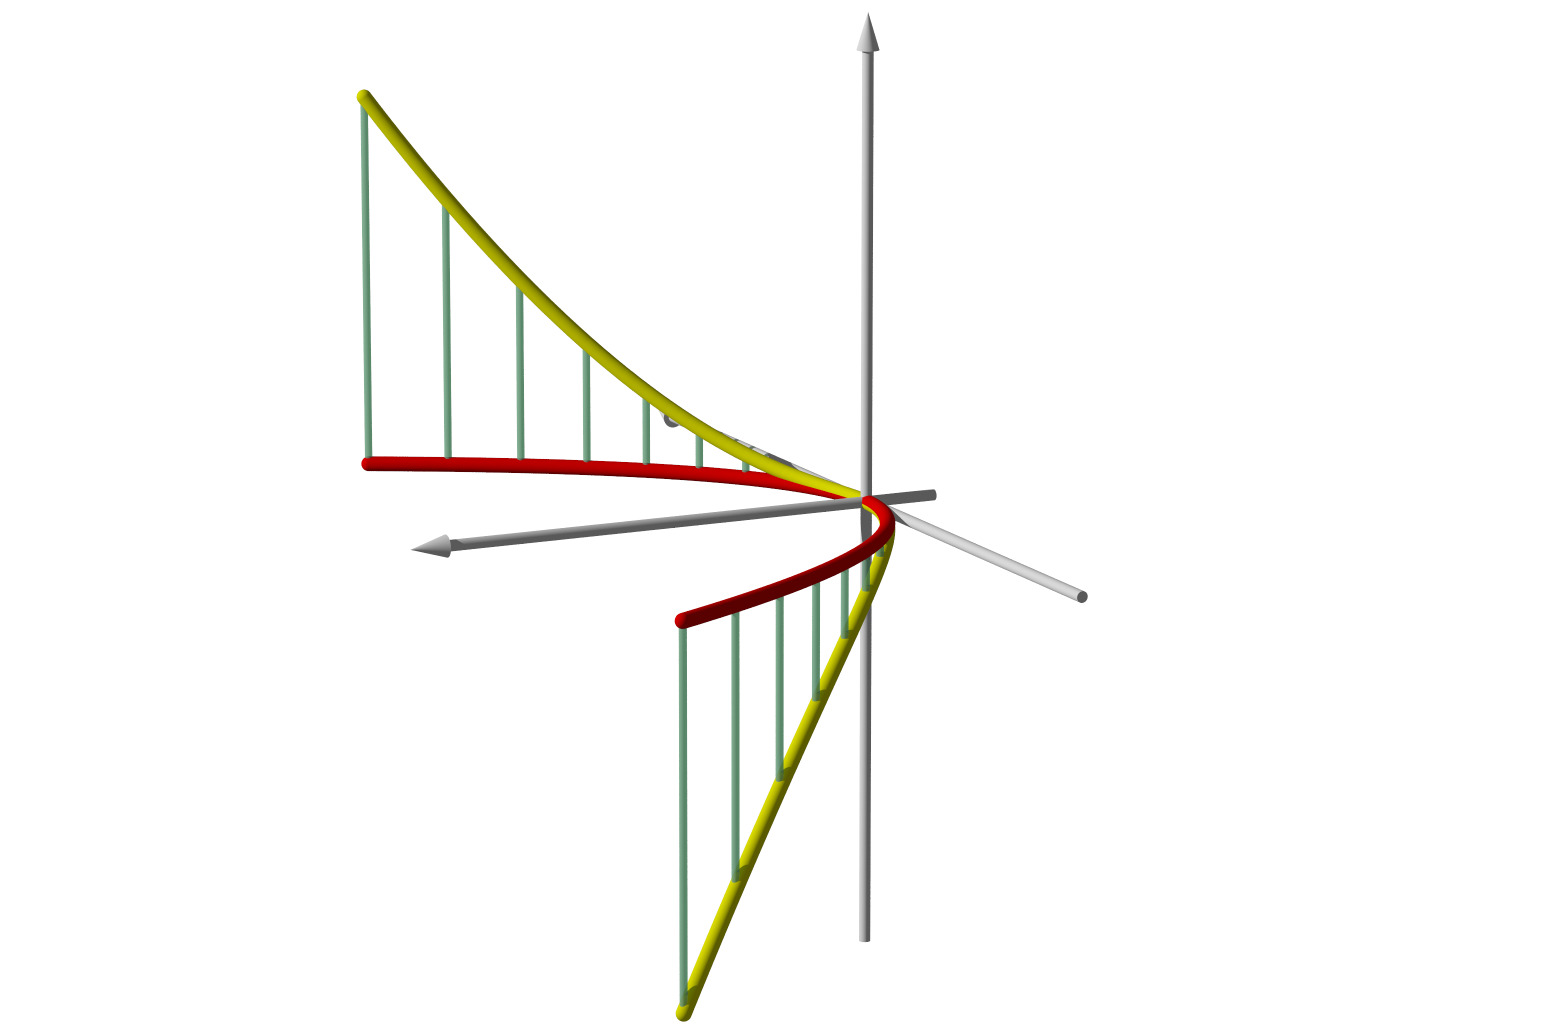
\includegraphics[width=\hsize]{chapters/3d/kurve.jpg}
\caption{Kurven $t\mapsto(t,t^2,0)$ (rot) und $t\mapsto(t,t^2,0)$ (geld).
\label{skript:kruemmung:fig:kurvekr}}
\end{figure}
Wir betrachten die beiden Kurven
\begin{align*}
c_1(t)&=(t,t^2,0)
&
c_2(t)&=(t,t^2,t^3)
\end{align*}
(Abbildgung~\ref{skript:kruemmung:fig:kurvekr}).
$c_1(t)$ ist eine ebene Kurve, nämlich die Projektion der Raumkurve
$c_2(t)$ in die $x$-$y$-Ebene, sie ist in
Abbildung~\ref{skript:kruemmung:fig:kurvekr} rot dargestellt.
Die Kurve $c_2(t)$ ist in Abbildung~\ref{skript:kruemmung:fig:kurvekr} 
dagegen gelb dargestellt.
Wir wollen von beiden Kurven die Krümmung berechnen.
Dazu berechnen wir zunächst die Ableitungen und das Vektorprodukt
\begin{align*}
\dot c_1(t)
&=
(1,2t,0)
&
\dot c_2(t)
&=
(1,2t,3t^2)
\\
\ddot c_1(t)
&=
(0,2,0)
&
\ddot c_2(t)
&=
(0, 2, 6t)
\\
\dot c_1(t)\times \ddot c_1(t)
&=
(0,0,2)
&
\dot c_2(t)\times \ddot c_2(t)
&=
(6t^2,-6t,2)
\end{align*}
Daraus kann man jetzt die Krümmungen berechnen:
\begin{align*}
\kappa_1(t)
&=
\frac{2}{(1+4t^2)^{\frac32}}
\\
\kappa_2(t)
&=
\frac{2}{(1+4t^2 + 9t^4)^{\frac32}}
\sqrt{1+9t^2+9t^4}
\end{align*}
Für den Parameterwert $t=0$ stimmen die beiden Krümmungen überein.
\end{beispiel}

\section{Rekonstruktion einer ebenen Kurve aus der Krümmung}
\rhead{Rekonstruktion aus der Krümmung}
Die Krümmung bestimmt eine Kurve eindeutig.
Umd dies einzusehen, parametrisieren wir eine ebene Kurve mit
$x$, schreiben also $c(x)=(x,y(x))$.
Wir müssen jetzt nachrechnen, dass die Vorgabe der Krümmung $\kappa(x)$
und der Steigung in einem Punkt die Kurve eindeutig festlegt.
Dazu stellen wir eine Differentialgleichung zweiter Ordnung auf,
allgemeine Sätze über Existenz und Eindeutigkeit der Lösung von
gewöhnlichen Differentialgleichungen werden unsere Aussage dann
als Konsequenz haben.

In dieser speziellen Wahl der Parametrisierung ist $\dot x = 1$ und
$\ddot x=0$.
Die Ableitung von $y$ nach dem Parameter ist dann $\dot y=y'(x)$.
Somit wird die Formel für die Krümmung
\[
\kappa(x)
=
\frac{\left|\begin{matrix}\dot x&\ddot x\\\dot y&\ddot y\end{matrix}\right|}{(\dot x^2+\dot y^2)^{\frac32}}
=
\frac{\left|\begin{matrix}1&0\\y'&y''\end{matrix}\right|}{(1+y'^2)^{\frac32}}
=
\frac{y''}{(1+y'(x))^{\frac32}}
\]
der in expliziter Form:
\[
y''(x)=\kappa(x) (1+y'(x)^2)^{\frac32}.
\]
Dies ist eine gewöhnliche Differentialgleichung zweiter Ordnung.
Da die rechte Seite erfüllt die Bedingungen, die in üblichen
Eindeutigkeitssätzen für gewöhnliche Differentialgleichungen
verlangt werden, daher gibt es genau eine Lösung dieser
Differentialgleichung zu vorgegebenem Anfangspunkt und Anfangsrichtung.
Damit ist gezeigt, dass in der Ebenen zwei Kurven mit der gleichen
Krümmung, gleichem Anfangspunkt und gleicher Anfangsrichtung übereinstimmen
müssen.
Anders formuliert: zwei ebene Kurven mit gleicher Krümmung in Abhängigkeit
von einem Bogenlängenparameter sind kongruent.

In drei Dimensionen kann die Krümmung allein eine Raumkurve nicht bestimmen.
Man kann dies zum Beispiel so einsehen.
Ist $c(t)$ eine gegeben Raumkurve, dann können wir deren Krümmung
$\kappa(t)$ berechnen.
In jeder Ebene durch den Punkt $c(0)$, die auch den Tangentenvektor
$\dot c(t)$ enthält, gibt es eine ebenen Kurve mit der gleichen
Krümmung $\kappa(t)$.
Da es unendlich viele solche Ebenen gibt, gibt es unendlich viele 
ebene Kurven, die die gleiche Krümmung haben wie die vorgegebene
Raumkurve.

Um eine Raumkurve eindeutig festzulegen braucht es daher ein weiteres
Datum, welches beschreibt, wie sich die aktuelle Tangentialebene
aufgespannt von $\dot c(t)$ und $\ddot c(t)$ dreht.
Diese {\em Torsion} genannt Grösse bestimmt dann die Kurve vollständig.
\index{Torsion}
Für eine ebene Kurve verschwindget die Torsion.

Die Kurventheorie lässt sich sogar auf eine beliebig grosse Zahl
von Dimensionen verallgemeinern.
Es stellt sich heraus, dass mit jeder zusätzlichen Dimension eine
zusätzliche Funktion Funktion notwendig wird.
Für eine Kurve in $n$ Dimensionen braucht es also $n-1$ Funktionen,
die beschreiben, wie sich ein entlang der Kurve mitbewegtes Koordinatensystem,
das sogenannte Frenet-$n$-Bein ändert.
\index{Frenet-$n$-Bein}
Diese Funktionen legen dann die Kurve bis auf die Wahl einer Anfangslage
des Koordinatensystem eindeutig fest.
Mit anderen Worten, wenn zwei Kurven in $n$ Dimensionen in den genannten
$n-1$ Funtionen übereinstimmen, dann sind sie kongruent.



%
% laengenmessung.tex -- Längenmessung in einer Fläche oder in einem Raum
%
% (c) 2017 Prof Dr Andreas Müller, Hochschule Rapperswil
%
\chapter{Längenmessung
\label{skript:kruemmung:section:laengenmessung}}
\lhead{Längenmessung}
\rhead{}

Die Physik seit Galileo und Newton machte die Annahme, dass die
Geometrie des Raumes durch ein dreidimensionales rechtwinkliges
Koordinatensystem mit der Längenmessungsformel
\begin{equation}
l=\sqrt{\Delta x^2+\Delta y^2+\Delta z^2}
\label{skript:kruemmung:pytagoras}
\end{equation}
adäquat beschrieben wird.
Diese Annahme entsprach zwar der Erfahrung, doch es gab keine
Begründung dafür.
Der Philosoph Emanuel Kant konnte sich zwar keine andere Geometrie
vorstellen, doch mit den Erkenntnissen von Bolyai, Lobaschevski
und Gauss wurde klar, dass es durchaus denkbare andere Geometrien
gibt.
Bernhard Riemann hat dann auch Methoden entwickelt, wie man die
Geometrie studieren kann, indem man ausschliesslich die Längenmessung
innerhalb des Raumes verwendet.
Damit ist die Geometrie unseres Raumes nicht länger einfach das
Resultat einer axiomatischen Beschreibung, wie Euklid sie gegeben hat,
vielmehr ist sie zu einer experimentellen Wissenschaft geworden.

Da wir nicht weiter annehmen wollen, dass sich der Raum mit Hilfe
eines rechtwinkligen Koordinatensystems adäquat beschreiben lässt,
müssen wir automatisch beliebige Koordinatensysteme zulassen.
Je nach Wahl eines Koordinatensystems werden dann Vektoren, die
wir für die Beschreibung der physikalischen Gesetze benötigen,
verschiedenen Koordinaten haben.
Da alle diese Koordinatensystem gleichberechtigt sind, müssen
wir Vektoren auf einheitliche Art umrechnen können.
Ausserdem müssen die Naturgesetze so formuliert sein, dass
sie in jedem beliebigen Koordinatensystem gleich aussehen.

In diesem Kapitel beginnen wir damit, den Begriff der Längenmessung
auf beliebige Koordinatensysteme auszudehnen.
Ein Punkt wird beschrieben durch seine Koordinaten, die wir mit
$x^\mu$ bezeichnen, wobei $\mu$ von $1$ bis $n$ läuft, $n$
ist die Dimension. 
Die etwas ungewohnte Schreibweise für die Indizes wie Exponenten
hat einen tieferen Grund in der Tensorrechnung, und wird später
verständlich werden.

\section{Vektoren und Koordinatentransformation}
\rhead{Vektoren und Koordinatentransformation}
Eine Koordinatentransformation zwischen zwei Koordinatensystemen ist
eine Abbildung, die die Koordinaten $x^\mu$ des einen Koordinatensystems
in die Koordinaten $y^\nu$ des anderen Koordinatensystems umrechnet.
Man kann also schreiben
\begin{equation}
y^{\nu}=y^{\nu}(x^1,\dots,x^n).
\label{skript:kruemmung:umrechnung}
\end{equation}
Uns interessiert vor allem die Beschreibung von Bahnkurven, wir möchten
ja zum Beispiel den Absturz in ein schwarzes Loch berechnen können.
Eine Bahnkurve erhält man, indem man die Koordinaten mit der Zeit
varieren lässt.
Eine Kurve wird also beschrieben durch Funktionen $x^\mu(t)$.

In der physikalischen Beschreibung werden meistens Vektoren wie
Geschwindigkeit und Beschleunigung verwendet.
Sie sind die Ableitung der Koordinaten eines Bahnpunktes nach
der Zeit.
Dies lässt sich direkt auch auf die Koordinaten übertragen,
wir erhalten für den Geschwindigkeitsvektor
\[
v^{\mu} = \frac{dx^\mu(t)}{dt}.
\]

Wie sieht der Geschwindigkeitsvektor in $y^{\nu}$ Koordinaten aus?
Dazu setzen wir die Bahnkurve in die Umrechnungsformeln
\eqref{skript:kruemmung:umrechnung} ein.
Die Kettenregel liefert
\begin{align*}
y^{\nu}(t)&=y^{\nu}(x^1(t),\dots,x^n(t))
\\
u^{\nu}
=
\frac{dy^{\nu}(t)}{dt}
&=
\frac{\partial y^{\nu}}{\partial x^1}\frac{dx^1(t)}{dt}
+\dots+
\frac{\partial y^{\nu}}{\partial x^n}\frac{dx^n(t)}{dt}
=
\sum_{\mu=1}^n
\frac{\partial y^{\nu}}{\partial x^{\mu}}\frac{dx^{\mu}(t)}{dt}
\end{align*}
Auf der rechten Seite steht eine Summe von Termen, in denen
der Summationsindex sowohl oben als auch unten auftritt.
Diese Art von Summe kommt in der zu entwickelnden Theorie sehr
häufig vor, daher schreiben wir in Zukunft die Summe nicht mehr.
Diese {\em Einsteinsche Summenkonvention} bedeutet also, dass in
einem Term, in dem der gleiche Index oben und unten vorkommt,
über die möglichen Werte dieses Index summiert werden muss.
\index{Summenkonvention!Einsteinsche}

Die Koeffizienten 
\[
\alpha_\mu^\nu=\frac{\partial y^{\nu}}{\partial x^{\mu}}
\]
dienen also der Umrechnung der Komponenten eines Vektors vom
$x^{\mu}$-Koordinatensystem ins $y^{\nu}$-Koordinatensystem.
Man kann die Rechnung auch in Matrixform schreiben:
\[
\begin{pmatrix}y^1\\\vdots\\y^n\end{pmatrix}
=
\begin{pmatrix}
\frac{\partial y^1}{\partial x^1}&\dots&\frac{\partial y^1}{\partial x^n}\\
\vdots&\ddots&\vdots\\
\frac{\partial y^n}{\partial x^1}&\dots&\frac{\partial y^n}{\partial x^n}
\end{pmatrix}
\begin{pmatrix}x^1\\\vdots\\x^n\end{pmatrix}.
\]
Die Summationskonvention lässt sich zum Beispiel dadurch rechtfertigen,
dass bei der Matrizenmultiplikation die Summation ja auch nicht
explizit hingeschrieben wird.

\section{Metrik}
\rhead{Metrik}
In einem rechtwinkligen Koordinatensystem können wir die Länge
einer Kurve durch Zerlegen in beliebig kleine Teilstücke 
\begin{align*}
l
&\simeq
\sum_{i=1}^n \sqrt{\sum_{\mu} (x^{\mu}(t_i)-x^{\mu}(t_{i-1}))^2}
\\
&\rightarrow
\int_{t_0}^{t_n} \sqrt{\sum_{\mu}\biggl(\frac{dx^{\mu}(t)}{dt}\biggr)^2}\,dt
\end{align*}
bestimmen.
Unter der Wurzel sehen wir die Quadratsummen wieder, die für den
Satz des Pythagoras charakteristisch sind.

In einem beliebigen Koordinatensystem funktioniert dies jedoch nicht
mehr.
Wir müssen zulassen, dass die Koordinaten entlang verschiedener
Achsen nicht mehr direkt der Länge entsprechen, dass wir also
entlang der Achsen Skalierungsfaktoren haben.
Weiter ist damit zu rechnen, dass auch gemischte Termen auftauchen.
Die allgemeinstmögliche Form einer Längenmessungsformel ist daher
\begin{equation}
l
=
\int_{t_0}^{t_1}
\sqrt{\sum_{\mu,\nu} g_{\mu\nu} \frac{dx^{\mu}(t)}{dt}\frac{dx^{\nu}(t)}{dt}}\,dt.
\label{skript:kruemmung:metrikformel}
\end{equation}
Die Zahlen $g_{\mu\nu}$ können dabei auch noch von den Koordinaten
abhängen.
Wir verlangen ausserdem, dass $g_{\mu\nu}=g_{\nu\mu}$ ist, denn
diese beiden Terme sind in \eqref{skript:kruemmung:metrikformel}
auf symmetrische Art und Weise vertreten.

\begin{definition}
Die Zahlen $g_{\mu\nu}$ heissen der metrische Tensor.
\index{Tensor!metrischer}
\end{definition}

Die Schreibweise~\eqref{skript:kruemmung:metrikformel} ist nicht
sehr handlich.
Wesentlich an der Notation ist einzig, wie die Koeffizienten $g_{\mu\nu}$
mit den Koordinateninkrementen $dx^\mu$ kombiniert werden müssen.
Wir können daher formal auch schreiben:
\[
ds^2
=
g_{\mu\nu}\,dx^\mu\,dx^\nu.
\]
Diese Notation ist konsistent, denn die Längenberechnung ist
\begin{equation}
\int\,ds
=
\int \sqrt{g_{\mu\nu}\,dx^\mu\,dx^\nu}
=
\int \sqrt{g_{\mu\nu}\,\dot x^\mu\,\dot x^\nu}\,dt,
\label{skript:kruemmung:laengenelement}
\end{equation}
wozu man einzig die Konvention braucht, dass man in Integralen
$dx^\mu=\dot x^\mu\,dt$ schreiben kann.
Man nennt \eqref{skript:kruemmung:laengenelement} das {\em Längenelement}
der Metrik $g_{\mu\nu}$.
\index{Längenelement}

%
% Beispiel für Längenmessung in einem Koordinatensystem mit nicht
% orthogonalen Achsen.
%
\begin{beispiel}
Wir untersuchen die Längenmessung mit nicht orthogonalen Achsen.
Statt des gewöhnlichen Koordinatensystems in einer Ebene verwenden
wir die Koordinaten $x'=x$ und $y'=x+y$.
In den ungestrichenen Koordinaten ist der Abstand zwischen zwei
Punkten durch den Satz von Pythagoras
\begin{equation}
l^2 = \Delta x^2 + \Delta y^2
\label{skript:kruemmung:p2}
\end{equation}
gegeben.
Um den Abstand in $x'$-$y'$-Koordinaten auszudrücken, müssen wir diese
erst wieder in $x$-$y$-Koordinaten umrechnen. 
Man findet
\[
x=x'
\qquad\text{und}\qquad
y=y'-x=y'-x'.
\]
Eingesetzt in die Formel \eqref{skript:kruemmung:p2} finden wir
\begin{align*}
l^2
&=
\Delta x^2 + \Delta y^2
=
\Delta x^{\prime 2}
+
(\Delta y'- \Delta x')^2
=
\Delta x^{\prime 2}
+
\Delta y^{\prime 2}-2\Delta x'\Delta y' + \Delta x^{\prime 2}
\\
&= 2 \Delta x^{\prime 2} - 2 \Delta x'\Delta y'+\Delta y^{\prime 2}.
\end{align*}
Die zugehörigen Koeffizienten $g_{\mu\nu}$ sind
\[
g_{11} = 2,\quad
g_{12}=g_{21}=-1\quad\text{und}\quad
g_{22}=1.
\]
Diese Koeffizienten beschreiben die gleiche Längenmessung in den 
gestrichenen Koordinaten wie der Satz von Pythagoras in den ursprünglichen
Koordinaten.
Man kann sie auch in der Form
\[
ds^2
=
dx^2+dy^2
=
2\,dx'^2-2\,dx'\,dy'+dy'^2
\]
als Längenelemente beschreiben.
\end{beispiel}

Die Formel \eqref{skript:kruemmung:metrikformel} ist etwas unhandlich.
Wir können aber wieder die Einsteinsche Summenkonvention verwenden,
um das Summenzeichen los zu werden.
Ausserdem kann man die Ableitungen nach $t$ auch mit einem Punkt abkürzen.
Damit lässt sich die Längenmessung daher etwas kompakter als
\[
l=\int_{t_0}^{t_1} \sqrt{g_{\mu\nu}\dot x^{\mu}(t) \dot x^{\nu}(t)}\,dt
\]
schreiben.

\section{Beispiele}
\rhead{Beispiele}
Wir betrachten drei für die Anwendungen wichtige Bespiele von
Koordinatensystemen des gewöhnlichen dreidimensionalen Raumes
und berechnen die zugehörigen metrischen Tensoren.

\subsection{Polarkoordinaten}
Punkte in der Ebene können statt in rechtwinkligen $x$-$y$-Koordinaten
auch mit Hilfe von Polarkoordinaten $(r,\varphi)$ nach der Umrechnungsregel
\begin{align*}
x&=r\cos\varphi\\
y&=r\sin\varphi
\end{align*}
beschrieben werden.
Um den metrischen Tensor zu bestimmen, müssen die Ableitungen von $x$ 
und $y$ nach $t$ durch Ableitungen von $r$ und $\varphi$ nach $t$ 
ausdrücken.
Die Produktregel liefert:
\begin{align*}
\dot x&= \dot r\cos \varphi - r\dot\varphi \sin\varphi 
\\
\dot y&= \dot r\sin\varphi + r\dot\varphi\cos\varphi.
\end{align*}
Eingesetzt in den Satz von Pythagoras folgt
\begin{align*}
\dot x^2 + \dot y^2
&=
\dot r^2\cos^2\varphi -2r\dot r\dot\varphi\cos\varphi\sin\varphi +r^2\dot \varphi^2\sin^2\varphi
+
\dot r^2\sin^2\varphi +2r\dot r\dot\varphi\sin\varphi\cos\varphi +r^2\dot\varphi^2\cos^2\varphi
\\
&=
\dot r^2(\cos^2\varphi+\sin^2\varphi)+ r^2\dot\varphi^2(\sin^2\varphi+\cos^2\varphi)
\\
&=\dot r^2 + r^2\dot\varphi^2.
\end{align*}
Die gemischten Terme haben sich weggehoben.
Man liest daraus für die Koeffizienten des metrischen Tensors
\[
g_{11}=1,\qquad g_{12}=g_{21}=0\qquad\text{und}\qquad g_{22}=r^2
\]
ab.
Das Längenelement in Polarkoordinaten ist daher
\[
ds^2
=
dr^2 + r^2\,d\varphi^2.
\]
\index{Längenelement!in Polarkoordinaten}
Die Koeffizienten hängen zwar von den Koordinaten ab, doch bedeutet
das noch nicht, dass ein gekrümmter Raum vorliegt.
Diese $g_{\mu\nu}$ beschreiben ja die gleiche Längenmessung wie der Satz
des Pythagoras in $x$-$y$-Koordinaten.

\subsection{Zylinderkoordinaten}
Zylinderkoordinaten beschreiben die Punkte des dreidimensionalen
Raumes mit Polarkoordinaten in der $x$-$y$-Ebene und der $z$-Koordinate.
Da wir die Metrik in der $x$-$y$-Ebene schon durch $(r,\varphi)$
ausgedrückt haben, können wir auch die Metrik in Polarkoordinaten
bekommen, indem wir die $z$-Koordinaten ergänzen:
\[
\dot x^2+\dot y^2 +\dot z^2
=
\dot r^2 + r^2\dot\varphi^2 + \dot z^2.
\]
Der zugehörige metrische Tensor hat daher die Koeffizienten
\[
g_{11}=1,\qquad
g_{22}=r^2
\qquad\text{und}\qquad
g_{33}=1,
\]
alle anderen Koeffizienten sind $0$.
Das Längenelement in Zylinderkoordinaten ist
\[
ds^2
=
dr^2+r^2\,d\varphi^2 + dz^2.
\]
\index{Längenelement!in Zylinderkoordinaten}

\subsection{Zylinderoberfläche}
Beschränken wir uns auf die Punkte im Abstand $1$ zur $z$-Achse, erhalten
wir eine Zylinderfläche, welche mit Koordinaten $\varphi$ und $z$
beschrieben werden kann.
Die Längenmessung in dieser Fläche wird durch den metrischen
Tensor der Zylinderkoordinaten beschrieben, in dem wir $r=1$ einsetzen.
Wir erhalten
\[
\dot\varphi^2+\dot z^2.
\]
Das Längenelement auf der Zylinderoberfläche $r=1$ mit den Koordinaten
$\varphi$ und $z$ ist daher
\[
ds^2
=
d\varphi^2+dz^2,
\]
\index{Längenelement!auf der Zylinderoberfläche}
die Koeffizienten des metrischen Tensors sind
\[
g_{11}=1,\qquad
g_{12}=g_{21}=0
\qquad\text{und}\qquad
g_{22}=1.
\]
Dies ist der metrische Tensor einer Ebene mit rechtwinkligen Koordinaten.
Daraus können wir bereits ablesen, dass die Zylinderoberfläche sich durch
Längenmessung nicht von einer Ebene unterscheiden lässt.

\subsection{Kugelkoordinaten}
Kugelkoordinaten beschreiben die Punkte eines dreidimensionalen Raumes
durch die Entfernung $r$ vom Nullpunkt, die geographische Länge
$\varphi$, die von
der $x$-Koordinate gemessen wird, und durch die geographische Breite
$\vartheta$,
die als Winkel von der $z$-Achse gemessen wird.
Die Umrechnung in kartesische Koordinaten erfolgt mit den Formeln
\begin{align*}
x&= r\sin\vartheta\cos\varphi\\
y&= r\sin\vartheta\sin\varphi\\
z&= r\cos\vartheta
\end{align*}
Wir bestimmen wieder die Koeffizienten des metrischen Tensors.
Dazu leiten wir zunächst nach $t$ ab.
\begin{align*}
\dot x
&=
\dot r\sin\vartheta\cos\varphi
+
r\dot\vartheta \cos\vartheta\cos\varphi
-
r\dot\varphi \sin\vartheta\sin\varphi
\\
\dot y
&=
\dot r\sin\vartheta\sin\varphi
+
r\dot\vartheta\cos\vartheta\sin\varphi
+
r\dot\varphi\sin\vartheta\cos\varphi
\\
\dot z
&=
\dot r\cos\vartheta
-
r\dot\vartheta \sin\vartheta
\end{align*}
Bei der Berechnung der Länge werden sich wieder viele Terme
wegen der verschiedenen Vorzeichen des letzten Terms im
Ausdruck für $\dot x$ und $\dot y$ aufheben.
Für den Ausdruck $ \dot x^2 + \dot y^2 + \dot z^2$ findet man
\[
\begin{array}{clclclcl}
 &
\dot r^2\sin^2\vartheta\cos^2\varphi
	&+&r^2\dot\vartheta^2\cos^2\vartheta\cos^2\varphi
		&+&r^2\dot\varphi^2\sin^2\vartheta\sin^2\varphi
			&+&2r\dot r\dot\vartheta\sin\vartheta\cos\vartheta\cos^2\varphi
\\
+&
\dot r^2\sin^2\vartheta\sin^2\varphi
	&+&r^2\dot\vartheta^2\cos^2\vartheta\sin^2\varphi
		&+&r^2\dot\varphi^2\sin^2\vartheta\cos^2\varphi
			&+&2r\dot r\dot\vartheta\sin\vartheta\cos\vartheta\sin^2\varphi
\\
+&
\dot r^2\cos^2\vartheta
	&+&r^2\dot\vartheta^2\sin^2\vartheta
		& &
			&-&2r\dot r\dot\vartheta \sin\vartheta \cos\vartheta
\\
\end{array}
\]
In den Spalten ergänzen sich in den ersten beiden Zeilen jeweils
$\cos^2\varphi$ und $\sin^2\varphi$ zu $1$.
In den ersten beiden Spalten lassen sich danach auch noch
$\cos^2\vartheta$ und $\sin^2\vartheta$ zu $1$ zusammenfassen,
während sich die Terme in der vierten Spalte aufheben.
Damit bekommt man
\begin{equation}
\dot x^2 + \dot y^2 + \dot z^2
=
\dot r^2+r^2\dot\vartheta^2 + r^2\dot\varphi^2\sin^2\vartheta
\label{skript:kruemmung:kugelkoordinaten}
\end{equation}
für die Längenmessung, und
\[
g_{11}=1,\qquad
g_{22}=r^2
\qquad\text{und}\qquad
g_{33}= r^2\sin^2\vartheta
\]
für die nicht verschwindenden Komponenten des metrischen Tensors.
Alternativ kann man dies auch als
\[
ds^2
=
dr^2 + r^2\,d\vartheta^2 + r^2\sin^2\vartheta\,d\varphi^2,
\]
also als Längenelement schreiben.
\index{Längenelement!in Kugelkoordinaten}

\subsection{Kugeloberfläche}
Aus dem metrischen Tensor der Kugelkoordinaten lässt sich durch festhalten
des Radius der metrische Tensor einer Kugeloberfläche ableiten.
Aus dem Ausruck \eqref{skript:kruemmung:kugelkoordinaten}
erhalten wir
\[
\dot\vartheta^2+\dot\varphi^2\sin^2\vartheta.
\]
Der $\sin$-Term deutet an, dass wir hier nicht mehr direkt eine flache
Metrik haben.
Den Nachweis können wir aber erst führen, wenn wir den Begriff der
Krümmung zur Verfügung haben.
Für die nicht verschwindenden Komponenten des metrischen Tensors
finden wir
\[
g_{11} = 1
\qquad\text{und}\qquad
g_{22}=\sin^2\vartheta.
\]
Etwas übersichtlicher ist 
\[
ds^2
=
d\vartheta^2 + \sin^2\vartheta\,d\varphi^2,
\]
das Längenelement auf der Kugeloberfläche.
\index{Längenelement!auf der Kugeloberfläche}
Man erkennt, dass der Koeffizient $g_{22}$ bei $\vartheta \in\{0,\pi\}$
verschwindet.
Man spricht von einer Singularität der Längenmessung.
Dies ist jedoch nur ein Artefakt der Tatsache, dass die Kugelkoordinaten
bei den Polen nicht mehr eindeutig sind.
Zur Beschreibung der Pole sind alle möglichen Werte der geographischen
Länge gleichermassen geeignet.

\section{Übungsaufgaben}
\rhead{Übungsaufgaben}
\uebungsaufgabe{0202}
\uebungsaufgabe{0203}
\uebungsaufgabe{0201}


%
% k-geodaeten.tex -- Gleichung der Geodäten, Christoffel-Symbole
%
% (c) 2017 Prof Dr Andreas Müller, Hochschule Rapperswil
%
\chapter{Geodäten
\label{skript:chapter:geodaeten}}
\lhead{Geodäten}
\rhead{}
In der Ebene ist die kürzeste Verbindung zwischen zwei Punkten
eine Gerade.
Auf einem Zylinder oder Kegel kann man die kürzeste Verbindung finden,
indem man die Fläche in eine Ebene abrollt, und dann dort verwendet,
dass die kürzeste Verbindung in der Ebene eine Gerade ist.
Dies zeigt, dass die kürzesten Verbindung nichts mit der speziellen
Einbettung einer Fläche zu tun hat, sondern eine Eigenschaft ist,
die sich allein aus der Längenmessung in der Fläche ist, man nennt
dies auch eine intrinsische Eigenschaft.

Auf einer Kugeloberfläche kann man die kürzesten Verbindungen ebenfalls
direkt angeben, es sind die Grosskreise.
\begin{figure}
\centering
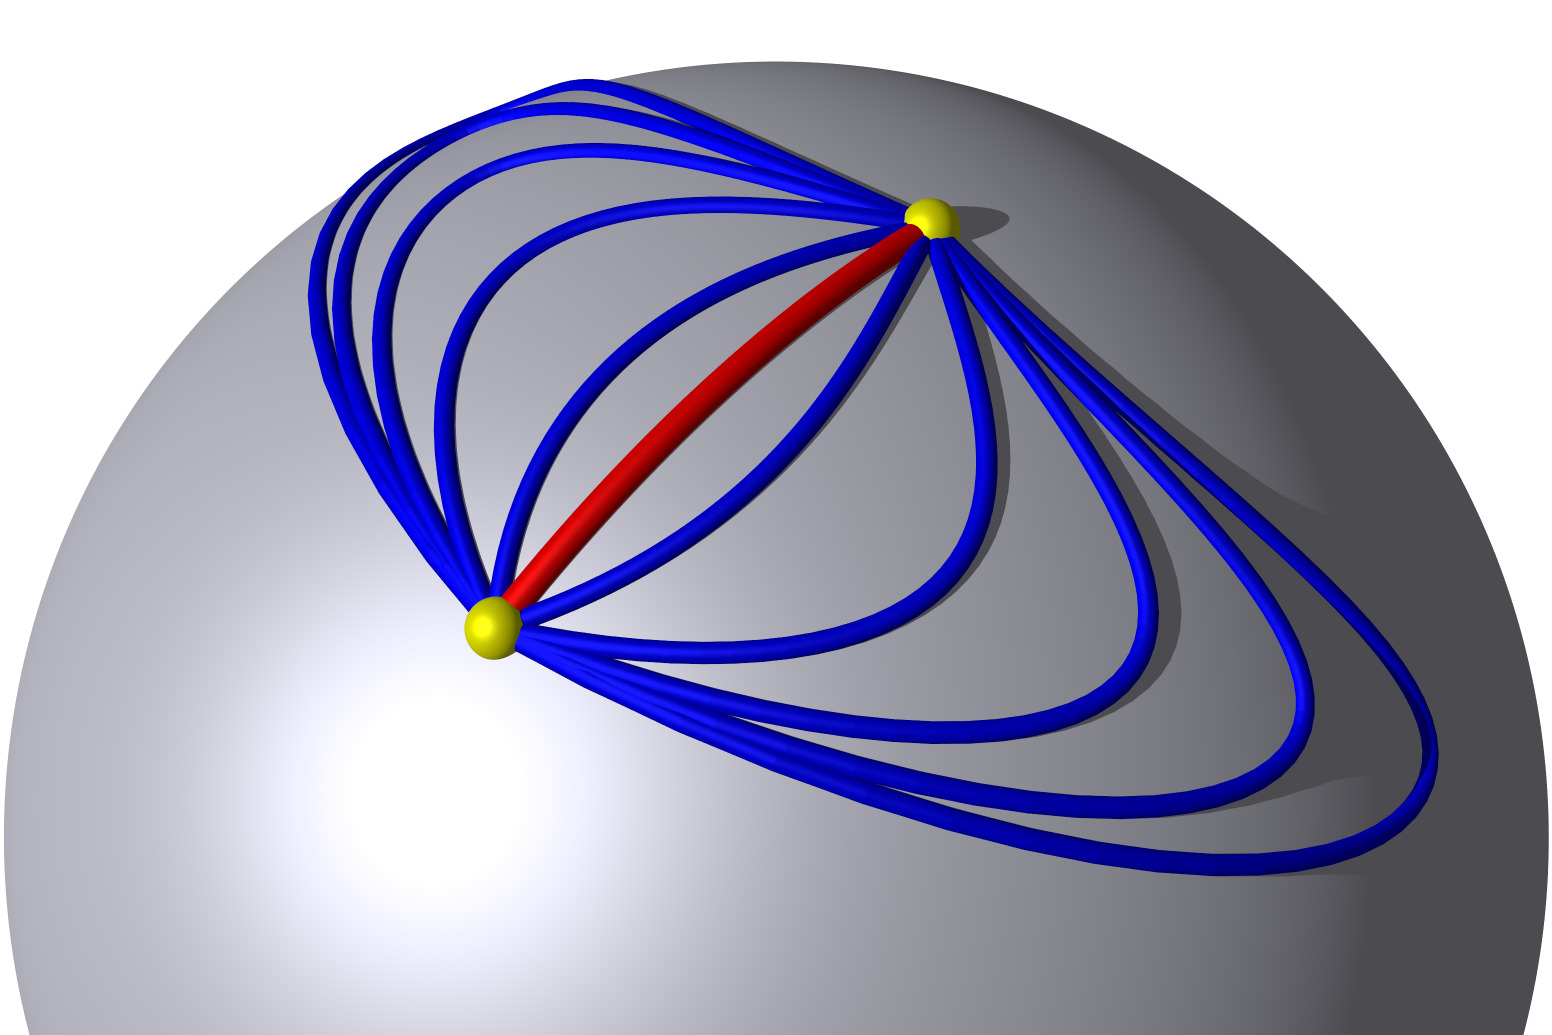
\includegraphics[width=\hsize]{chapters/3d/geodaete.jpg}
\caption{Ein Ausschnitt aus einem Grosskreis (rot) ist die kürzestmögliche
Verbindung zwischen zwei Punkten auf einer Kugeloberfläche.
Alle anderen Kurven (blau) in der Kugeloberfläche haben grössere Länge.
\label{skript:kruemmung:fig:geodaete}}
\end{figure}
Man kann dabei so argumentieren: von allen Schnitten der Kugeloberfläche
mit Ebenen durch die zwei gegeben Punkte ist der Grosskreis derjenige
mit der kleinsten Krümmung, und daher die ``direkteste'' Verbindung.
Dieses Argument ist allerdings nicht ganz exakt, denn man vergisst dabei,
dass es noch viele weitere Kurven gibt, die die beiden Punkte verbinden
(Abbildung~\ref{skript:kruemmung:fig:geodaete}).
Es ist auch nicht wirklich auf noch allgemeinere Situationen übertragbar,
denn es nützt aus, dass die Kugeloberfläche homogen ist, in jedem Punkt
ist die ``Krümmung'' (ein im Moment noch nicht definierter Begriff) 
gleich gross.

Auch die Ausbreitung des Lichts in einem Medium ist einer solchen
Beschreibung zugänglich.
Das Licht wählt immer den Weg mit der geringsten Laufzeit, nicht
unbedingt den geometrisch kürzesten Weg.
Daher können sich Lichtstrahlen in einem inhomogenen Medium
krümmen.
Aus der Perspektive des Lichtes ist aber nicht die Bahn gekrümmt,
es folgt der in dieser Geometrie geradest möglichen Bahn.
Nicht die Bahn ist gekrümmt, sondern die Längenmessung weicht von
der üblichen \eqref{skript:kruemmung:pytagoras} ab, der Raum ist
gekrümmt.

In diesem Abschnitt suchen wir daher nach einer allgemeinen Methode,
die kürzeste Verbindung, die sogenannten Geodäten zu finden.

\section{Paralleltransport}
\rhead{Paralleltransport}
\begin{figure}
\centering
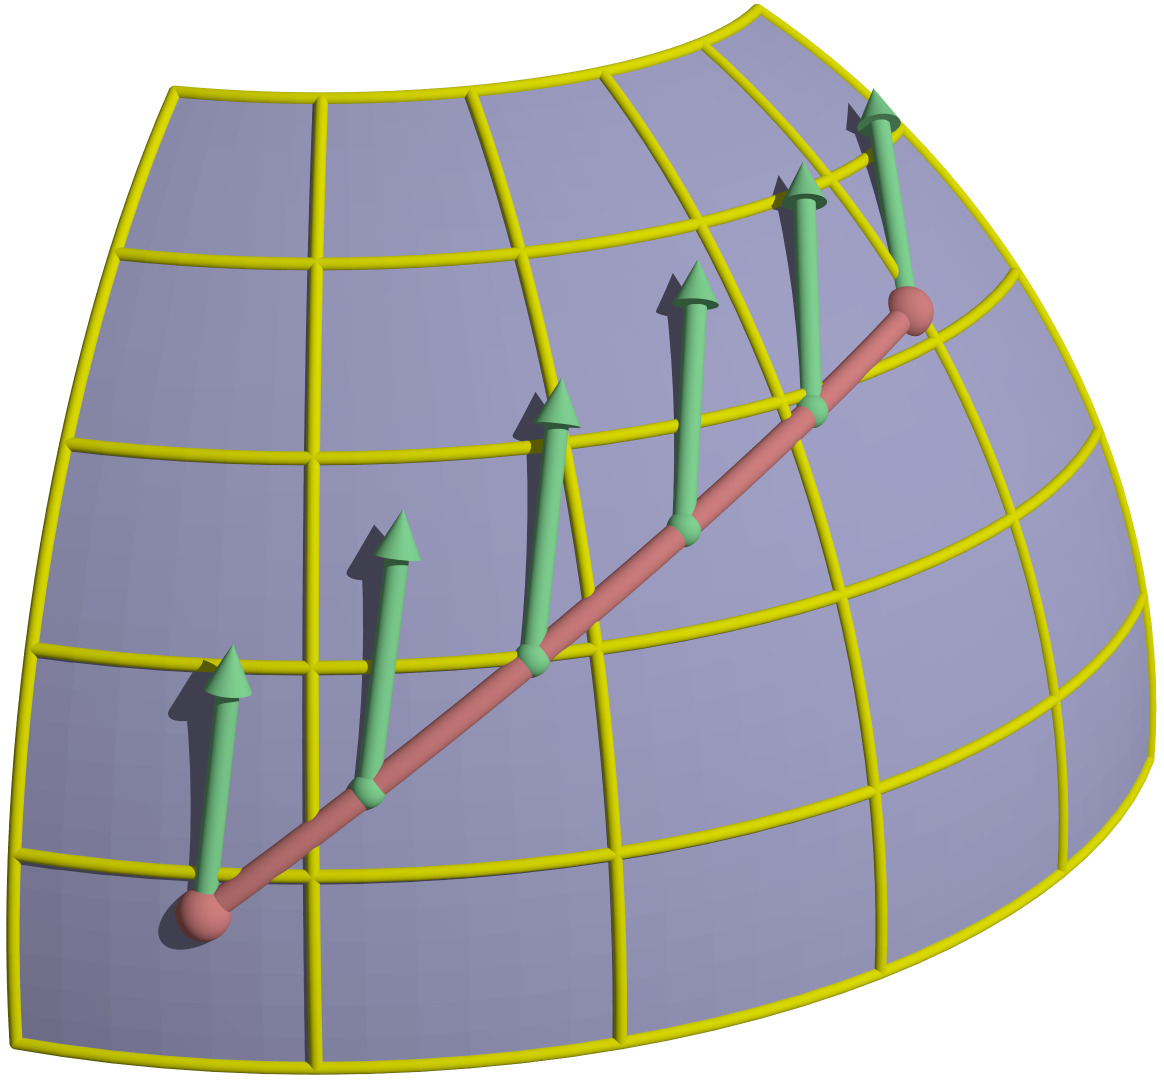
\includegraphics[width=\hsize]{chapters/3d/transport.jpg}
\caption{Paralleltransport eines Vektors entlang einer Kurve auf
einer Kugeloberfläche%
\label{skript:geodaten:fig:transport}}
\end{figure}
Die Beispiele von kürzesten Verbindungen suggerieren, dass die kürzeste
Verbindung auch die ``geradeste'' ist, sie weicht möglichst wenig von
der Richtung des aktuellen Tangentialvektors ab.
Das Problem bei dieser Interpretation ist allerdings, dass wir Vektoren
in zwei verschiedenen Punkten der Fläche nicht unmittelbar vergleichen
können.
Auf der Kugeloberfläche liegen die Tangentialvektoren an eine Kurve in
verschiedenen Punkten zum Beispiel in verschiedenen Tangentialebenen
an die Kugel.

Wir müssen also zunächst in der Lage sein, Vektoren in zwei verschiedenen
Punkten miteinander zu vergleichen.
Wir können das tun, indem wir einen Vektor entlang einer Kurve transportieren,
wobei wir versuchen, in so parallel zu sich selbst wie möglich zu sich
selbst zu halten (Abbildung~\ref{skript:geodaten:fig:transport}).
Auch dies ist im Moment noch ein etwas schwammiger Begriff. 
Es ist aber klar, dass die Komponenten des transportierten Vektors
sowohl von der Transportrichtung wie auch vom ursprünglichen Vektor
abhängen.

Seien $A^\mu$ die Komponenten eines Vektors, die Richtung mit Komponenten
$\Delta x^\nu$ transport werden soll.
Wenn wir uns entlang einer Kurve in diese Richtung bewegen, werden sich
die Komponenten $A^\mu$ einfach deshalb ändern, weil die Komponenten von
den Koordinaten abhängig sind.
Bei einem paralleltransportierten Vektor wird ein Teil dieser Änderung
komponsiert auf geeignete Art komponsiert sein müssen.
Die Kompensation wird linear vom Vektor $A^\mu$ und von der
Bewegungsrichtung abhängen.
Wir schreiben dafür
\[
\nabla_\nu A^\mu\cdot \Delta x^\nu
=
\biggl(\frac{\partial A^\mu}{\partial x^\nu}
+
\Gamma^\mu_{\alpha\nu}A^\alpha\biggr)\Delta x^\nu.
\]
Die Funktionen $\Gamma^\mu_{\alpha\nu}$ sind vorerst noch nicht bekannt,
wir werden sie noch bestimmen müssen.

\begin{definition}
Die {\em kovariante Ableitung} eines Vektorfeldes $A^\mu$ ist der 
\index{kovariante Ableitung}
\index{Ableitung, kovariante}
Ausdruck
\begin{equation}
\nabla_\nu A^\mu
=
\frac{\partial A^\mu}{\partial x^\nu}
+
\Gamma^\mu_{\alpha\nu}A^\alpha,
\label{skript:geodaeten:kovarianteableitung}
\end{equation}
die Koeffizienten $\Gamma^\mu_{\alpha\nu}$ heissen Christoffelsymbole
zweiter Art oder Zusammenhangskoeffizienten.
Eine weiter verbreitete Schreibweise für die kovariante Ableitung
ist
\[
\nabla_\nu A^\mu
=
A^\mu\mathstrut_{;\nu}.
\]
\end{definition}

Die kovariante Ableitung soll ausdrücken, wie sich die Komponenten eines
Vektors entlang einer Kurve ändern, unabhängig von der konkreten Wahl
des Koordinatensystems.
Paralleltransport soll heissen, dass sich entlang einer Kurve die
Komponenten eines Vektors nicht ändern,
dass also $\nabla_\nu A^\mu=0$.
Insbesondere möchten wir später den Tangentialvektor einer Kurve entlang
der Kurve selbst transportieren.
Die kovariante Ableitung des Tangentialvektors $\dot x^\mu$ entlang
einer Kurve wird dann sein
\[
\nabla_\nu\dot x^\mu
=
\frac{\partial \dot x^\mu}{\partial x^\nu}
+
\Gamma^\mu_{\alpha\nu}\dot x^\alpha
\]
und die zeitliche Änderung entlang der Kurve wird
\[
\nabla_\nu\dot x^\mu\cdot \dot x^\nu
=
\frac{\partial \dot x^\mu}{\partial x^\nu}\dot x^\nu
+
\Gamma^\mu_{\alpha\nu}\dot x^\alpha \dot x^\nu.
\]
Im letzten Ausdruck kommen $x^\alpha$ und $x^\nu$ in symmetrischer
Art und Weise vor.
Dies suggeriert, dass wir die $\Gamma^\mu_{\alpha\nu}$ möglicherweise
sogar symmetrisch wählen können, dass also
$\Gamma^\mu_{\alpha\nu}=\Gamma^\mu_{\nu\alpha}$
gewählt werden kann.
Wir fordern daher zusätzlich, dass die Zusammenhangskoeffizienten
symmetrisch sein sollen.
Es wird sich gleich zeigen, dass dies tatsächlich möglich ist.

Bis jetzt haben wir die Metrik nicht verwendet.
Wir möchten, dass der Paralleltransport die Länge des Vektors beim
Transport entlang einer Kurve nicht verändert.
Die Länge des Vektors wird durch $g_{\mu\nu}\tilde A^\mu \tilde A^\nu$
gegeben.
Die Ableitung entlang der Kurve $x^\mu(t)$ ist
\[
\frac{d}{dt} g_{\mu\nu}\tilde A^\mu \tilde A^\nu\bigg|_{t=0}
=
\frac{\partial g_{\mu\nu}}{\partial x^\alpha}A^\mu A^\nu\dot x^\alpha
-
g_{\mu\nu}A^\mu\Gamma_{\alpha\beta}^\nu A^\alpha \dot x^\beta
-
g_{\mu\nu}\Gamma_{\alpha\beta}^\mu A^\alpha \dot x^\beta A^\nu
=
0.
\]
In diesem Ausdruck kommen in allen Termen $A^\mu$ und $\dot x^\beta$ mit
verschiedenen Indizes vor.
Damit wir diese Faktoren ausklammern können, benennen wir die Indizes um,
so dass sie in allen Termen gleich sind.
Wir erhalten dann die Gleichung
\[
\biggl(
\frac{\partial g_{\mu\nu}}{\partial x^\alpha}
-
g_{\mu\beta}\Gamma_{\nu\alpha}^\beta
-
g_{\beta\nu}\Gamma_{\mu\alpha}^\beta
\biggr)
A^\mu A^\nu\dot x^\alpha
=
0
\]
F"ur die Koeffizienten $\Gamma$.
Diese Gleichung muss f"ur jede beliebige Wahl von $A^\mu$ und jede
beliebige Richtung der Kurve $\dot x^\alpha$ erfüllt sein, wenn der
Klammerausdruck verschwindet für alle Werte der freien, also nicht durch
die Summationskonvention als Laufindizes ausgezeichneten, Indizes.
Wir erhalten also
\begin{equation}
\frac{\partial g_{\mu\nu}}{\partial x^\alpha}
-
g_{\mu\beta}\Gamma_{\nu\alpha}^\beta
-
g_{\beta\nu}\Gamma_{\mu\alpha}^\beta
=
0,
\label{skript:geodaeten:gammaidentitaet}
\end{equation}
ein System von Gleichungen für die $n^3$ Grössen $\Gamma_{\mu\nu}^\alpha$.
Wir können die $\Gamma$ auch allein auf der linken Seite haben:
\[
g_{\mu\beta}\Gamma_{\nu\alpha}^\beta
+
g_{\beta\nu}\Gamma_{\mu\alpha}^\beta
=
\frac{\partial g_{\mu\nu}}{\partial x^\alpha}
\]
Durch zyklische Vertauschung der drei Indizes $\mu$, $\nu$ und $\alpha$
erhalten wir drei Gleichungen
\[
\def\arraystretch{2.0}
\begin{linsys}{3}
g_{\mu\beta}\Gamma_{\nu\alpha}^\beta &+& g_{\beta\nu}\Gamma_{\mu\alpha}^\beta
& &
&=&
\displaystyle
\frac{\partial g_{\mu\nu}}{\partial x^\alpha}
\\
& &g_{\nu\beta}\Gamma_{\alpha\mu}^\beta &+& g_{\beta\alpha}\Gamma_{\nu\mu}^\beta
&=&
\displaystyle
\frac{\partial g_{\nu\alpha}}{\partial x^\mu}
\\
g_{\beta\mu}\Gamma_{\alpha\nu}^\beta
& &
&+&g_{\alpha\beta}\Gamma_{\mu\nu}^\beta 
&=&
\displaystyle
\frac{\partial g_{\alpha\mu}}{\partial x^\nu}
\end{linsys}
\]
Da sowohl $g$ als auch $\Gamma$ in den unteren Indizes symmetrisch
sind, können wir die Gleichungen weiter vereinfachen:
\[
\def\arraystretch{2.0}
\begin{linsys}{3}
g_{\mu\beta}\Gamma_{\nu\alpha}^\beta
	&+& g_{\nu\beta}\Gamma_{\mu\alpha}^\beta
		& &
&=&
\displaystyle
\frac{\partial g_{\mu\nu}}{\partial x^\alpha}
\\
	& &g_{\nu\beta}\Gamma_{\mu\alpha}^\beta
		&+& g_{\alpha\beta}\Gamma_{\nu\mu}^\beta
&=&
\displaystyle
\frac{\partial g_{\nu\alpha}}{\partial x^\mu}
\\
g_{\mu\beta}\Gamma_{\nu\alpha}^\beta
	& &
		&+&g_{\alpha\beta}\Gamma_{\nu\mu}^\beta 
&=&
\displaystyle
\frac{\partial g_{\alpha\mu}}{\partial x^\nu}
\end{linsys}
\]
Subtrahieren wir die erste Zeile von der Summe der letzten beiden,
heben sich ersten Terme weg, es bleibt
\[
g_{\alpha\beta}\Gamma_{\nu\mu}^\beta
=
\biggl(
\frac{\partial g_{\nu\alpha}}{\partial x^\mu}
+
\frac{\partial g_{\alpha\mu}}{\partial x^\nu}
-
\frac{\partial g_{\mu\nu}}{\partial x^\alpha}
\biggr).
\]
Bezeichen wir die inverse Matrix von $g_{\alpha\beta}$ mit
$g^{\alpha\beta}$, dann k"onnen wir nach $\Gamma_{\mu\nu}^\beta$ aufl"osen:
\[
g^{\sigma\alpha}
\biggl(
\frac{\partial g_{\nu\alpha}}{\partial x^\mu}
+
\frac{\partial g_{\alpha\mu}}{\partial x^\nu}
-
\frac{\partial g_{\mu\nu}}{\partial x^\alpha}
\biggr)
=
g^{\sigma\alpha}
g_{\alpha\beta}\Gamma_{\mu\nu}^\beta
=
\delta^\sigma_\beta\Gamma_{\mu\nu}^\beta
=
\Gamma_{\mu\nu}^\sigma.
\]

\begin{definition}
Sei $g_{\mu\nu}$ ein metrischer Tensor. 
Dann heissen die
\[
\Gamma_{\alpha,\mu\nu}
=
\frac12
\biggl(
\frac{\partial g_{\nu\alpha}}{\partial x^\mu}
+
\frac{\partial g_{\alpha\mu}}{\partial x^\nu}
-
\frac{\partial g_{\mu\nu}}{\partial x^\alpha}
\biggr)
\]
die {\em Christoffelsymbole 1.~Art}
und
\begin{equation}
\Gamma_{\mu\nu}^\sigma
=
g^{\sigma\alpha} \Gamma_{\alpha,\mu\nu}
=
\frac12
g^{\sigma\alpha}
\biggl(
\frac{\partial g_{\nu\alpha}}{\partial x^\mu}
+
\frac{\partial g_{\alpha\mu}}{\partial x^\nu}
-
\frac{\partial g_{\mu\nu}}{\partial x^\alpha}
\biggr)
\label{skript:definition:christoffel2}
\end{equation}
heissen {\em Christoffelsymbole 2.~Art} oder {\em Zusammenhangskoeffizienten}.
Die auf diese Weise aus der Metrik gewonnenen Zusammenhangskoeffizienten
sind auch als der
{\em Levi-Cività-Zusammenhang} bekannt.
\index{Levi-Cività-Zusammenhang}
\end{definition}

\section{Rechenregeln für die kovariante Ableitung}
\rhead{Kovariante Ableitung}
Die kovariante Ableitung eines Vektorfeldes wurde in 
\eqref{skript:geodaeten:kovarianteableitung}
für ein Vektorfeld $A^\mu$ definiert.
Später wurden die Koeffizienten $\Gamma^\alpha_{\mu\nu}$ so bestimmt,
dass der Paralleltransport, der als geometrische Vorstellung der
Formel~\eqref{skript:geodaeten:kovarianteableitung} zu Grunde lag,
Skalarprodukte erhält.
Für zwei Vektorfelder, die beide verschwindende
kovariante Ableitung in beine bestimmte Richtung haben,
verschwindet dann auch die Ableitung in diese Richtung.
Doch wie verhält sich die Ableitung eines Skalarprodukts, wenn
die einzelnen Faktoren nicht verschwindende kovariante Ableitung haben?
Ziel dieses Abschnittes ist, Rechenregeln für die kovariante Ableitung
zusammenzustellen.

Wir betrachten zwei Vektorfelder $A^\mu$ und $B^\mu$ und möchten wissen,
wie sich der Wert des Skalarproduktes $g_{\mu\nu}A^\mu B^\nu$ entlang
einer Kurve mit Tangentenrichtung $C^\mu$ ändert.
Seien $A^\mu$  und $B^\nu$ beliebige Vektorfelder,
dann gilt entlang einer Kurve mit
Richtungsvektor $C^\mu$ im Punkt mit Parameterwert $s=0$
\begin{align*}
\frac{d}{ds}(g_{\mu\nu}A^\mu B^\nu)\bigg|_{s=0}
&=
\frac{\partial g_{\mu\nu}}{\partial x^\alpha}A^\mu B^\nu
+
g_{\mu\nu}\frac{\partial A^\mu}{\partial x^\alpha}C^\alpha B^\nu
+
g_{\mu\nu}A^\mu \frac{\partial B^\nu}{\partial x^\alpha}C^\alpha
\\
&=
\biggl(
\frac{\partial g_{\mu\nu}}{\partial x^\alpha}C^\alpha A^\mu B^\nu
+
g_{\mu\nu}
\biggl(\nabla_\alpha A^\mu - \Gamma^\mu_{\beta\alpha}A^\beta \biggr)
B^\nu
+
g_{\mu\nu}A^\mu \biggl(\nabla_\alpha B^\nu-\Gamma^\nu_{\beta\alpha}B^\beta\biggr)
\biggr)C^\alpha
\\
&=
C^\alpha
\biggl(
g_{\mu\nu}\nabla_\alpha A^\mu B^\nu
+
g_{\mu\nu}A^\mu\nabla_\alpha B^\nu
+
\biggl(
\frac{\partial g_{\mu\nu}}{\partial x^\alpha}
-g_{\beta\nu}\Gamma^\beta_{\mu\alpha}
-g_{\mu\beta}\Gamma^\beta_{\nu\alpha}
\biggr)A^\mu B^\nu
\biggr)
\end{align*}
Der innere Klammerausdruck in der letzten Gleichung ist aber identisch
mit \eqref{skript:geodaeten:gammaidentitaet}, er verschwindet also.
Damit können wir die Komponenten Ableitung in Richtung $C^\mu$ auch
so schreiben:
\[
\frac{\partial}{\partial x^\alpha}
(g_{\mu\nu}A^\mu B^\nu)
=
g_{\mu\nu}\nabla_\alpha A^\mu B^\nu
+
g_{\mu\nu}A^\mu\nabla_\alpha B^\nu,
\]
dies ist die Produktregel für die kovariante Ableitung.

\begin{satz}
Für zwei beliebige Vektorfelder sind die Komponenten der Ableitung
des Skalarproduktes 
\begin{equation}
\frac{\partial}{\partial x^\alpha}
(g_{\mu\nu}A^\mu B^\nu)
=
g_{\mu\nu}\nabla_\alpha A^\mu B^\nu
+
g_{\mu\nu}A^\mu\nabla_\alpha B^\nu.
\label{skript:geodaeten:produktregel}
\end{equation}
\end{satz}

Bis jetzt können wir nur die kovariante Ableitung von Vektorkomponenten
$A^\mu$ berechnen, eine kovariante Ableitung von Komponenten $B_\nu$
ist noch gar nicht definiert.
Wir können aber jeden Vektor $B_\nu$ also das Resultat einer Operation
$B_\nu=B^\alpha g_{\alpha\nu}$ betrachten.
Das Skalarprodukt $A^\mu B_\mu=A^\mu B^\nu g_{\mu\nu}$ erfüllt dann
wieder die Produktregel~\eqref{skript:geodaeten:produktregel},
als
\[
\frac{\partial}{\partial x^\alpha}A^\mu B_\mu
=
\frac{\partial}{\partial x^\alpha}g_{\mu\nu} A^\mu B^\nu
=
g_{\mu\nu} \nabla_\alpha A^\mu B^\nu
+
g_{\mu\nu} A^\mu \nabla_\alpha B^\nu
=
\nabla_\alpha A^\mu B_\mu
+
A^\mu g_{\mu\nu} \nabla_\alpha B^\nu.
\]
Wenn die kovariante Ableitung für $B_\nu$ überhaupt definiert werden 
kann, dann muss gelten
\begin{align}
\nabla_\alpha B_\nu
&=
g_{\mu\nu}\nabla_\alpha B^\mu
\notag
\\
&=
g_{\mu\nu}\frac{\partial B^\mu}{\partial x^\alpha}
+
g_{\mu\nu}\Gamma^\mu_{\alpha\beta}B^\beta
\notag
\\
&=
g_{\mu\nu}\frac{\partial g^{\mu\beta}B_\beta}{\partial x^\alpha}
+
g_{\mu\nu}\Gamma^\mu_{\alpha\beta}g^{\beta\sigma}B_\sigma
\notag
\\
&=
g_{\mu\nu}\frac{\partial g^{\mu\beta}}{\partial x^\alpha} B_\beta
+
\underbrace{g_{\mu\nu}g^{\mu\beta}}_{=\delta_\nu^\beta}\frac{\partial B_\beta}{\partial x^\alpha}
+
g_{\mu\nu}\Gamma^\mu_{\alpha\beta}g^{\beta\sigma}B_\sigma
\notag
\\
&=
\frac{\partial B_\nu}{\partial x^\alpha}
+
g_{\mu\nu}\biggl(
\frac{\partial g^{\mu\sigma}}{\partial x^\alpha}
+\Gamma^\mu_{\alpha\beta}g^{\beta\sigma}
\biggr)B_\sigma
\label{skript:geodaeten:kovkov1}
\end{align}
Die Ableitungen der inversen Matrix $g^{\mu\sigma}$ berechnen wir
durch Ableiten der Bedingung $\delta_\nu^\sigma=g_{\nu\mu}g^{\mu\sigma}$:
\begin{equation}
0
=
\frac{\partial}{\partial x^\alpha}\delta_\nu^\sigma
=
\frac{\partial g_{\mu\nu}}{\partial x^\alpha} g^{\mu\sigma}
+
g_{\mu\nu}
\frac{\partial g^{\mu\sigma}}{\partial x^\alpha}
\qquad\Rightarrow\qquad
g_{\mu\nu}
\frac{\partial g^{\mu\sigma}}{\partial x^\alpha}
=
-
\frac{\partial g_{\mu\nu}}{\partial x^\alpha} g^{\mu\sigma}.
\label{skript:geodaeten:ginvabl}
\end{equation}
Setzen wir jetzt~\eqref{skript:geodaeten:ginvabl}
in~\eqref{skript:geodaeten:kovkov1} ein, erhalten wir
\begin{align*}
\nabla_\alpha B_\nu
&=
\frac{\partial B_\nu}{\partial x^\alpha}
+
\biggl(
-\frac{\partial g_{\mu\nu}}{\partial x^\alpha} g^{\mu\sigma}
+
g_{\mu\nu}
\Gamma^\mu_{\alpha\beta}g^{\beta\sigma}
\biggr)B_\sigma
\end{align*}
In der Klammer ersetzen wir $\Gamma^\mu_{\alpha\beta}$ durch
\eqref{skript:definition:christoffel2} und erhalten
\begin{align*}
-\frac{\partial g_{\mu\nu}}{\partial x^\alpha} g^{\mu\sigma}
+
g_{\mu\nu}
\Gamma^\mu_{\alpha\beta}
g^{\beta\sigma}
&=
-\frac{\partial g_{\mu\nu}}{\partial x^\alpha} g^{\mu\sigma}
+
g_{\mu\nu}
\frac12
g^{\mu\gamma}
\biggl(
\frac{\partial g_{\alpha\gamma}}{\partial x^\beta}
+
\frac{\partial g_{\beta\gamma}}{\partial x^\alpha}
-
\frac{\partial g_{\alpha\beta}}{\partial x^\gamma}
\biggr)
g^{\beta\sigma}
\\
&=
\biggl(
-\frac{\partial g_{\beta\nu}}{\partial x^\alpha} g^{\beta\sigma}
+
\delta_\nu^\gamma
\frac12
\biggl(
\frac{\partial g_{\alpha\gamma}}{\partial x^\beta}
+
\frac{\partial g_{\beta\gamma}}{\partial x^\alpha}
-
\frac{\partial g_{\alpha\beta}}{\partial x^\gamma}
\biggr)
\biggr)
g^{\beta\sigma}
\\
&=
\frac12
\biggl(
-2\frac{\partial g_{\beta\nu}}{\partial x^\alpha} g^{\beta\sigma}
+
\frac{\partial g_{\alpha\nu}}{\partial x^\beta}
+
\frac{\partial g_{\beta\nu}}{\partial x^\alpha}
-
\frac{\partial g_{\alpha\beta}}{\partial x^\nu}
\biggr)
g^{\beta\sigma}
\\
&=
-\frac12
\biggl(
\frac{\partial g_{\beta\nu}}{\partial x^\alpha}
+
\frac{\partial g_{\alpha\beta}}{\partial x^\nu}
-
\frac{\partial g_{\alpha\nu}}{\partial x^\beta}
\biggr)
g^{\beta\sigma}
\\
&=-\Gamma^\sigma_{\alpha\nu}
\end{align*}
\begin{definition}
Die Komponenten der kovariante Ableitung $\nabla_\alpha B_\nu$ eines
kovarianten Vektorfeldes $B_\nu$ in Richtung der Koordinaten $x^\alpha$
ist
\begin{equation}
\nabla_\alpha B_\nu
=
\frac{\partial B_\nu}{\partial\alpha}
-\Gamma^{\sigma}_{\alpha\nu}B_\sigma,
\label{skript:geodaeten:kovabl2}
\end{equation}
Diese wird auch $\nabla_\alpha B_\nu=B_{\nu;\alpha}$ geschrieben.
\end{definition}

\section{Beispiele}
\rhead{Beispiele}
In den nachfolgenden Beispielen wollen wir die Christoffelsymbole erster
und zweiter Art für Zylinder- und Kugeloberfläche berechnen.

\subsection{Polarkoordinaten}
Die nicht verschwinden Komponenten
des metrischen Tensors in Polarkoordinaten $(r,\varphi)$
sind $g_{11}=1$ und $g_{22}=r^2$.
Davon brauchen wir die Ableitungen
\[
\begin{aligned}
\frac{\partial g_{11}}{\partial x^1} &=0,&
\frac{\partial g_{12}}{\partial x^1} &=0,&
\frac{\partial g_{21}}{\partial x^1} &=0,&
\frac{\partial g_{22}}{\partial x^1} &=2r,&
\\
\frac{\partial g_{11}}{\partial x^2} &=0,&
\frac{\partial g_{12}}{\partial x^2} &=0,&
\frac{\partial g_{21}}{\partial x^2} &=0,&
\frac{\partial g_{22}}{\partial x^2} &=0
\end{aligned}
\]
Die Christoffelsymbole erster Art sind daher 
\[
\begin{aligned}
\Gamma_{1,11} &=  0,&
\Gamma_{1,12} &=  0,&
\Gamma_{1,21} &=  0,&
\Gamma_{1,22} &= -r,
\\
\Gamma_{2,11} &=  0,&
\Gamma_{2,12} &=  r,&
\Gamma_{2,21} &=  r,&
\Gamma_{2,22} &=  0
\end{aligned}
\]
und die Christoffelsymbole zweiter Art sind
\begin{equation}
\begin{aligned}
\Gamma_{11}^1 &= 0,&
\Gamma_{12}^1 &= 0,&
\Gamma_{21}^1 &= 0,&
\Gamma_{22}^1 &=-r,
\\
\Gamma_{11}^2 &= 0,&
\Gamma_{12}^2 &= \frac1{r},&
\Gamma_{21}^2 &= \frac1{r},&
\Gamma_{22}^2 &= 0.
\end{aligned}
\label{skript:geodaeten:christoffel:polar}
\end{equation}

\subsection{Zylinderkoordinaten}
Da die Komponenten des metrischen Tensors sind konstant, damit verschwinden
alle Ableitungen
\[
\frac{\partial g_{\mu\nu}}{\partial x^\alpha}=0
\qquad\Rightarrow\qquad
\Gamma_{\alpha,\mu\nu}=0
\qquad\Rightarrow\qquad
\Gamma_{\mu\nu}^\alpha=0.
\]

\subsection{Kugelkoordinaten}
Die Kugeloberfläche verwendet die Koordinaten $(\vartheta,\varphi)$.
Zun"achst brauchen wir die Ableitungen der Komponenten des metrischen
Tensors
\begin{align*}
\frac{\partial g_{11}}{\partial \vartheta} &=0,
&
\frac{\partial g_{12}}{\partial \vartheta} &=0,
&
\frac{\partial g_{21}}{\partial \vartheta} &=0,
&
\frac{\partial g_{22}}{\partial \vartheta} &=\sin2\vartheta,
\\
\frac{\partial g_{11}}{\partial \varphi} &=0,
&
\frac{\partial g_{12}}{\partial \varphi} &=0,
&
\frac{\partial g_{21}}{\partial \varphi} &=0,
&
\frac{\partial g_{22}}{\partial \varphi} &=0.
\\
\end{align*}
Daraus können wir die Christoffelsymbole erster Art ableiten:
\begin{align*}
 \Gamma_{1,11}
&=
\frac12\biggl(\frac{\partial g_{11}}{\partial \vartheta}
	+ \frac{\partial g_{11}}{\partial \vartheta}
	- \frac{\partial g_{11}}{\partial \vartheta}\biggr)=0,
&\Gamma_{1,12}
&=
\frac12\biggl(\frac{\partial g_{11}}{\partial \varphi}
	+ \frac{\partial g_{21}}{\partial \vartheta}
	- \frac{\partial g_{12}}{\partial \vartheta}\biggr)=0,
\\
\Gamma_{1,21}
&=
\frac12\biggl(\frac{\partial g_{12}}{\partial \vartheta}
	+ \frac{\partial g_{11}}{\partial \varphi}
	- \frac{\partial g_{21}}{\partial \vartheta}\biggr)=0,
&\Gamma_{1,22}
&=
\frac12\biggl(\frac{\partial g_{12}}{\partial \varphi}
	+ \frac{\partial g_{12}}{\partial \varphi}
	- \frac{\partial g_{22}}{\partial \vartheta}\biggr)=-\frac12\sin2\vartheta,
\\
\Gamma_{2,11}
&=
\frac12\biggl(\frac{\partial g_{12}}{\partial \vartheta}
	+ \frac{\partial g_{12}}{\partial \vartheta}
	- \frac{\partial g_{11}}{\partial \varphi}\biggr)=0,
&\Gamma_{2,12}
&=
\frac12\biggl(\frac{\partial g_{12}}{\partial \varphi}
	+ \frac{\partial g_{22}}{\partial \vartheta}
	- \frac{\partial g_{12}}{\partial \varphi}\biggr)=\frac12\sin2\vartheta,
\\
\Gamma_{2,21}
&=
\frac12\biggl(\frac{\partial g_{12}}{\partial \varphi}
	+ \frac{\partial g_{22}}{\partial \vartheta}
	- \frac{\partial g_{21}}{\partial \varphi}\biggr)=\frac12\sin2\vartheta,
&\Gamma_{2,22}
&=
\frac12\biggl(\frac{\partial g_{22}}{\partial \varphi}
	+ \frac{\partial g_{22}}{\partial \varphi}
	- \frac{\partial g_{22}}{\partial \varphi}\biggr)=0.
\end{align*}
Die inverse Matrix von $g_{\mu\nu}$ hat die nicht verschwindenden
Komponenten
\[
g^{11} = 1
\qquad\text{und}\qquad
g^{22} = \frac1{\sin^2\vartheta}
\]
und die Christoffelsymbole 2.~Art
\begin{equation}
\begin{aligned}
 \Gamma_{11}^1
&=0,
&\Gamma_{12}^1
&=0,
&\Gamma_{21}^1
&=0,
&\Gamma_{22}^1
&=-\frac12\sin2\vartheta,
\\
 \Gamma_{11}^2
&=0,
&\Gamma_{12}^2
&=\cot\vartheta,
&\Gamma_{21}^2
&=\cot\vartheta,
&\Gamma_{22}^2
&=0.
\end{aligned}
\label{skript:kruemmung:christoffelkugel}
\end{equation}


\section{Geodätengleichung}
\rhead{Geodätengleichung}
Die Rolle der Geraden in der Ebene müssen diejenigen Kurven auf der
Fläche übernehmen, die so gerade wie möglich sind. 
Eine Gerade ist dadurch charakterisiert, dass sie überall die gleiche
Richtung hat. 
Diese Formulierung ist aber nur möglich, weil Tangentialvektoren in
beliebigen Punkten unmittelbar miteinander vergleichen können.
Für einen allgemeinen Raum müssen wir diesen Vergleich mit Hilfe
des Paralleltransportes durchführen.
Die Forderung an die Kurve wird dann, dass der Tangentialvektor
an die Kurve durch Paralleltransport wieder in einen Tangentialvektor
an die Kurve übergeht.

Etwas formaler setzen wir den Tangentialvektor $\dot x^\mu$ an die
Kurve in die Gleichung \eqref{skript:kruemmung:ableitung} ein und
erhalten die Differentialgleichung 
\begin{equation}
\ddot x^\alpha+\Gamma_{\mu\nu}^\alpha \dot x^\mu\dot x^\nu=0.
\label{skript:kruemmung:geodatengleichung}
\end{equation}
\index{Geodäte}

\begin{definition}
Eine Kurve in einem Riemannschen Raum heisst eine Geodäte, wenn sie
die Differentialgleichung~\eqref{skript:kruemmung:geodatengleichung}
erfüllt.
\end{definition}

In den nachfolgenden Beispielen wollen wir die Geodäten für diejenigen
Räume berechnen, für die wir die Christoffelsymbole bereits bestimmt
haben.

%
% XXX Geschwindigkeitsinvarianz
%

\subsection{Flache R"aume}
In flachen Räumen wie der Ebene oder der Zylinderoberfläche verschwinden
alle Christoffelsymbole.
Die Geodätengleichung ist daher nur noch
$\ddot x^\alpha=0$, was gleichbedeutend ist mit
\[
x^\alpha(t)=x^\alpha(0) + t \dot x^\alpha(0),
\]
also einer Geradengleichung.
In flachen Räumen sind die Geodäten Geraden.

\subsection{Polarkoordinaten}
Die Geodätengleichungen in Polarkoordinaten erhält man durch
Einsetzen der Christoffelsymbole von
\eqref{skript:geodaeten:christoffel:polar}
in
\eqref{skript:kruemmung:geodatengleichung}.
Die Gleichungen lauten
\begin{equation}
\begin{aligned}
\ddot r &= r\dot \varphi^2,
\\
\ddot \varphi &= -2\frac{\dot r}{r}\dot\varphi.
\end{aligned}
\label{skript:geodaeten:dglpolar}
\end{equation}
Radiale Geraden haben $\dot\varphi=0$, aus der ersten Gleichung folgt dann
$\ddot r=0$ oder $\dot r=\operatorname{const}$.
Geodäten durch den Nullpunkt sind also mit konstanter Geschwindigkeit
durchlaufene Geraden.

Wir dürfen natürlich davon ausgehen, dass jede beliebige andere Gerade
ebenfalls eine Geodäte ist.
Um dies nachzuprüfen betrachten wir eine Gerade senkrecht auf die
$r=0$-Achse, in $x$-$y$-Koordinaten können wir sie als
$t\mapsto (x_0,t)$ beschreiben.
Die zugehörigen Polarkoordinaten sind
\[
\begin{aligned}
r(t)&=\sqrt{x_0^2+t^2}
&&\text{und}&
\varphi(t)&=\arctan\frac{t}{x_0}.
\end{aligned}
\]
Wir prüfen durch einsetzen, ob diese Funktionen die
Geodätendifferentialgleichung~\eqref{skript:geodaeten:dglpolar}
erfüllen.
Die Ableitungen von $r(t)$ und $\varphi(t)$ sind
\begin{align*}
\dot r(t)
&=\frac{t}{r},
&
\ddot r(t)
&=
\frac{1}{r}-\frac{t^2}{r^3}
=
\frac{r^2-t^2}{r^3}
=
\frac{x_0^2}{r^3},
\\
\dot\varphi(t)
&=
\frac{x_0}{r^2},
&
\ddot\varphi(t)
&=
-\frac{2tx_0}{r^4}.
\end{align*}
Setzen wir dies in die
Differentialgleichungen~\eqref{skript:geodaeten:dglpolar}
ein, erhalten wir
\begin{align*}
r\dot\varphi^2
&=
r\frac{x_0^2}{r^4}
=
\frac{x_0^2}{r^3}
=
\ddot r,
\\
-2\frac{\dot r}{r}\dot\varphi
&=
-2\frac{t}{r}\frac1{r}\frac{x_0}{r^2}
=
-\frac{2tx_0}{r^4}
=
\ddot\varphi.
\end{align*}
Wie erwartet erfüllt also die Gerade die Geodätengleichung.

\subsection{Kugeloberfläche}
Die Christoffelsymbole zweiter Art für die Kugeloberfläche haben wir
in \eqref{skript:kruemmung:christoffelkugel} berechnet.
Statt die Differentialgleichung der Geodäten direkt zu lösen, versuchen
wir nur, die Parameterdarstellung eines Grosskreises in die
Differentialgleichung einzusetzen und damit zu zeigen, dass die
Grosskreise Lösungen der Geodätengleichung sind.
Da es durch jeden Punkt der Kugeloberflächen und zu jeder Tangentialrichtung
einen Grosskreis gibt, und die Lösungen der Geodätengleichung eindeutig
sind, können wir schliessen, dass alle Geodäten Grosskreise sind.

Der Äquator der Kugel hat eine besonders einfache Parametrisierung mit
\[
\begin{aligned}
x^1(t)=\vartheta(t)&=\frac{\pi}2,
&\qquad&&
x^2(t)=\varphi(t)&=t
\end{aligned}
\]
mit den Ableitungen
\[
\begin{aligned}
\dot x^1(t)&=0,
&\qquad&&
\dot x^2(t)&=1.
\end{aligned}
\]
Die zweiten Ableitungen der Koordinaten verschwinden, da die ersten
Ableitungen konstant sind.
Wir setzen die ersten Ableitungen in die Geodätengleichung ein.
Es bleiben nur die Terme mit $\mu=\nu=2$ stehen, da $\dot x^1=0$ ist,
also
\begin{align}
\ddot x^1
&=
-\Gamma_{\mu\nu}^1\dot x^\mu\dot x^\nu
=
-\Gamma_{22}^1=\frac12\sin2\theta
=
\frac12\sin\biggl( 2\cdot\frac{\pi}2\biggr)
=
\frac12\sin\pi
=
0,
\label{skript:kruemmung:geodaete:breitenkreis}
\\
\ddot x^2
&=
-\Gamma_{\mu\nu}^2\dot x^\mu\dot x^\nu
=
-\Gamma_{22}^2=0.
\notag
\end{align}
Die Geodätengleichung ist für den Äquator erfüllt, der Äquator ist
eine Geodäte.

An dieser Stelle könnten wir mit den Rechnungen eigentlich aufhören, 
denn jeder andere Grosskreis entsteht aus dem Äquator durch eine
Drehung des dreidimensionalen Raumes.
Die Eigenschaft einer Kurve, eine Geodäte zu sein, hängt aber nur von
der Metrik ab, die sich bei einer solchen Drehung nicht ändert.
Jeder andere Grosskreis ist also automatisch auch eine Geodäte.
Trotzdem wollen wir im folgenden für jeden beliebigen Grosskreis
zeigen, dass er die Differentialgleichung der Geodäten erfüllt.

Ein Breitenkreis ist nach der gleichen Rechnung keine Geodäte.
Er ist charakterisiert durch $x^1(t)=\vartheta(t)\ne\frac{\pi}2$,
die Differentialgleichung
\eqref{skript:kruemmung:geodaete:breitenkreis}
wird damit zu
\[
\ddot x^1
=
-\Gamma_{\mu\nu}^1\dot x^\mu\dot x^\nu
=
-\Gamma_{22}^1
=
\frac12\sin2\theta
\ne
0,
\]
die Differentialgleichung der Geodäten ist nicht erfüllt.
Die rechte Seite ist sogar konstant, dies besagt dass der Breitenkreis
im Bezug zu einer Geodäten so gekrümmt ist, dass er ganz
auf einer Seite des Grosskreises mit gleichem Anfangspunkt und
Anfangsgeschwindigkeit liegt.

Als nächstes betrachten wir die Meridiane der Kugel.
Ein Meridian hat die Parameterdarstellung
\[
\begin{aligned}
x^1(t)=\vartheta(t)&=t,
&\qquad&&
x^2(t)=\varphi(t)&=0.
\end{aligned}
\]
Die Tangentialvektoren sind daher
\[
\begin{aligned}
\dot x^1(t)&=1,
&\qquad&&
\dot x^2(t)&=0.
\end{aligned}
\]
Wiederum verschwinden
die zweiten Ableitungen von $x^\mu$.
Wir setzen dies jetzt in die Geodäten\-gleichung ein und erhalten
\begin{align*}
\ddot x^1
&=
-\Gamma_{\mu\nu}\dot x^\mu \dot x^\nu
=
-\Gamma_{22}^1\dot x^2 \dot x^2
=
0,
\\
\ddot x^2
&=
-\Gamma_{\mu\nu}^2\dot x^\mu \dot x^\nu
=
-\Gamma_{11}^2\dot x^1\dot x^1
=
-\Gamma_{11}^2
=
0.
\end{align*}
Die Differentialgleichungen für eine Geodäte sind für Meridiane erfüllt,
damit ist gezeigt, dass Meridiane Geodäten sind.

Die Berechnung für einen beliebigen Grosskreis ist dagegen sehr 
kompliziert und nicht sehr instruktiv.

\section{Variationsprinzip}
\rhead{Variationsprinzip}
Wir möchten in diesem Abschnitt verstehen, dass die Geodäten tatsächlich 
die kürzesten Kurven sind.
Dazu müssen wir für eine beliebige mit dem Parameter $t$ parametrisierte
Kurve $x^\alpha(t)$ die Länge berechnen.
Dies kann mit dem Integral
\begin{equation}
l=\int_{t_0}^{t_1} \sqrt{g_{\mu\nu}(x^\alpha(t)) \dot x^\mu(t)\dot x^\nu(t)}\,dt
\label{skript:variation:laenge}
\end{equation}
geschehen.
Gesucht wird jetzt unter allen möglichen Kurven, die zwei Punkte miteinander
verbinden, diejenige für die das Integral \eqref{skript:variation:laenge}
minimal wird.

\subsection{Euler-Lagrange-Gleichung}
\begin{figure}
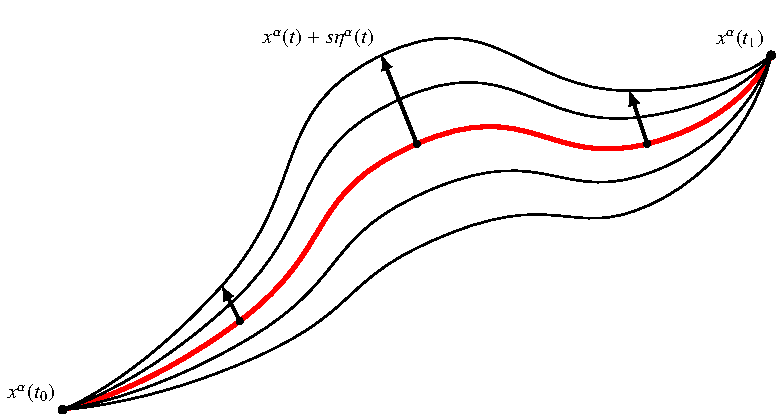
\includegraphics{chapters/tikz/lagrange.pdf}
\caption{Nachbarkurven der Lösungskurve eines Variationsproblems
für die Herleitung der Euler-Lagrange-Gleichung.
\label{skript:geodaeten:fig:lagrange}}
\end{figure}
Wir lösen gleich ein etwas allgemeineres Problem.
Gegeben ist eine Funktion $F(x^\alpha, \dot x^\alpha, t)$, welche
von den Koordinaten $x^\mu$, den Geschwindigkeiten $\dot x^\mu$ und
der Zeit abhängt.
Gesucht ist eine Kurve $x^\alpha(t)$, welche 
den Punkt $x^\alpha(t_0)$ mit dem Punkt $x^\alpha(t_1)$ verbindet,
und das Integral
\begin{equation}
\int_{t_0}^{t_1} F(x^\alpha(t), \dot x^\alpha(t), t)\,dt
\label{skript:variation:funktional}
\end{equation}
minimiert.

Wenn $x^\alpha(t)$ das Integral \eqref{skript:variation:funktional}
minimiert, dann wird es grösser, wenn man die Kurve etwas ändert.
Wir wählen also eine Kurve $\eta^\alpha(t)$ und berechnen, die
um $\eta^\mu(t)$ verschobene Kurve wird ein grösseres Integral
\eqref{skript:variation:funktional} ergeben.
Wir bilden daher
\[
I(s)
=
\int_{t_0}^{t_1}
F(x^\alpha(t) + s\eta^\alpha(t), \dot x^\alpha(t) + s \dot \eta^\alpha(t), t)
\,dt.
\]
Dieses Integral soll minimal werden für $s=0$, also muss die Ableitung
dort verschwinden.
Wir leiten daher nach $s$ ab:
\begin{align*}
\frac{dI(s)}{ds}
&=
\int_{t_0}^{t_1}
\frac{\partial F}{\partial x^\alpha}(x^\alpha(t)+s\eta^\alpha(t),
\dot x^\alpha(t) + s\dot\eta^\alpha(t), t) \eta^\alpha(t)
+
\frac{\partial F}{\partial \dot x^\alpha}(x^\alpha(t) + s\eta^\alpha(t),
\dot x^\alpha(t) + s\dot\eta^\alpha(t), t) \dot\eta^\alpha(t)
\,dt
\\
\frac{dI(0)}{ds}
&=
\int_{t_0}^{t_1}
\frac{\partial F}{\partial x^\alpha}(x^\alpha(t), \dot x^\alpha(t), t)
\eta^\alpha(t)
+
\frac{\partial F}{\partial \dot x^\alpha}(x^\alpha(t),
\dot x^\alpha(t), t)
\dot\eta^\alpha(t)
\,dt
\\
\intertext{
Den zweiten Term können wir mit partieller Integration vereinfachen
und erhalten}
&=
\int_{t_0}^{t_1}
\frac{\partial F}{\partial x^\alpha}(x^\alpha(t), \dot x^\alpha(t), t)
\eta^\alpha(t)\,dt
+
\biggl[
\frac{\partial F}{\partial \dot x^\alpha}(x^\alpha(t),
\dot x^\alpha(t), t)
\eta^\alpha(t)
\biggr]_{t_0}^{t_1}
\\
&\qquad\qquad
-
\int_{t_0}^{t_1}
\frac{d}{dt}\frac{\partial F}{\partial \dot x^\alpha}(x^\alpha(t),
\dot x^\alpha(t), t)
\eta^\alpha(t)
\,dt
\intertext{Da die verschobene Kurve immer noch die beiden Punkte
$x^\alpha(t_0)$ und $x^\alpha(t_1)$ verbindet, ist $\eta^\alpha(t_0)=0$
und $\eta^\alpha(t_1)=0$, und damit verschwindet der mittlere Term.
Die rechte Seite wird damit zu}
&=
\int_{t_0}^{t_1}
\biggl(
\frac{\partial F}{\partial x^\alpha}(x^\alpha(t), \dot x^\alpha(t), t)
-
\frac{d}{dt}\frac{\partial F}{\partial \dot x^\alpha}(x^\alpha(t),
\dot x^\alpha(t), t)
\biggr)
\eta^\alpha(t)
\,dt
\end{align*}
Das Integral auf der rechten Seite verschwindet nur dann für jede
beliebige Wahl der Verschiebung $\eta^\alpha(t)$, wenn die grosse Klammer
verschwindet.
Eine Lösung des Minimalproblems erfüllt also notwendigerweise die
sogenannten {\em Euler-Lagrange-Gleichungen}
\index{Euler-Lagrange-Gleichungen}%
\[
\frac{\partial F}{\partial x^\alpha}(x^\alpha(t), \dot x^\alpha(t), t)
-
\frac{d}{dt}\frac{\partial F}{\partial \dot x^\alpha}(x^\alpha(t), \dot x^\alpha(t), t)=0.
\]
Etwas kompakter geschrieben lauten diese
\begin{equation}
\frac{\partial F}{\partial x^\alpha}
-
\frac{d}{dt}\frac{\partial F}{\partial \dot x^\alpha}
=0.
\label{skript:variation:euler-lagrange}
\end{equation}

\subsection{Parametrisierung}
Wir vermuten, dass Geodäten die kürzesten Verbindungen sind.
Mit den Euler-Lagrange-Gleichungen können wir dies nachprüfen.
Wenn die Vermutung stimmt, müssten die Euler-Lagrange-Gleichungen 
\eqref{skript:variation:euler-lagrange}
für die Funktion
\[
L(x^\alpha, \dot x^\beta) =\sqrt{g_{\mu\nu}(x^\alpha)\dot x^\mu\dot x^\nu}
\]
die Differentialgleichungen der Geodäten liefern.
Wegen der Wurzel ist allerdings damit zu rechnen, dass die
Ableitungen, die wir für die Euler-Lagrange-Gleichungen brauchen sehr
kompliziert werden.

Die Geodäten-Gleichungen haben aber noch eine zusätzliche Eigenschaft.
Wir sind nämlich davon ausgegangen, dass der Tangentialvektor (der
Geschwindigkeitsvektor) immer die gleiche Länge hat, dass also
\[
\frac{d}{dt}L=0.
\]
Unter Verwendung dieser Eigenschaft können wir die Euler-Lagrange-Gleichung
wesentlich vereinfachen.
Dazu schreiben wir zunächst
\[
F=\frac12 L^2
\]
und berechnen die partiellen Ableitungen mit der Kettenregel:
\[
\begin{aligned}
\frac{\partial F}{\partial x^\alpha}
&=
L
\frac{\partial L}{\partial x^\alpha}
&&\text{und}
&
\frac{\partial F}{\partial \dot x^\alpha}
&=
L\frac{\partial L}{\partial\dot x^\alpha}
\end{aligned}
\]
Damit können wir jetzt die Euler-Lagrange-Gleichungen für $F$ aufstellen:
\begin{align*}
\frac{d}{dt}
\frac{\partial F}{\partial \dot x^\alpha}
&=
\frac{dL}{dt} \frac{\partial L}{\partial\dot x^\alpha}
+
L\frac{d}{dt}\frac{\partial L}{\partial\dot x^\alpha}
\\
\frac{d}{dt}
\frac{\partial F}{\partial \dot x^\alpha}
-
\frac{\partial F}{\partial x^\alpha}
&=
\underbrace{\frac{dL}{dt}}_{\displaystyle =0}
\frac{\partial L}{\partial\dot x^\alpha}
+
L\frac{d}{dt}\frac{\partial L}{\partial\dot x^\alpha}
-
L
\frac{\partial L}{\partial x^\alpha}
=
L\biggl(
\frac{d}{dt}\frac{\partial L}{\partial\dot x^\alpha}
-
\frac{\partial L}{\partial x^\alpha}
\biggr)
\end{align*}
Die Klammer auf der rechten Seite ist die Euler-Lagrange-Gleichung für
$L$.
Wenn wir also $dL/dt=0$ voraussetzen, dann ist die Euler-Lagrange-Gleichung
für $L$ gleichbedeutend mit der Euler-Lagrange-Gleichung für $F$.

\subsection{Lagrange-Gleichung für Geodäten}
Wir suchen jetzt also die Euler-Lagrange-Gleichungen f"ur die Funktion
\[
F(x^\alpha, \dot x^\alpha) = \frac12 g_{\mu\nu} \dot x^\mu \dot x^\nu.
\]
Wir berechnen daher die Ableitungen
\begin{align*}
\frac{\partial F}{\partial x^\alpha}
&=
\frac12\frac{\partial g_{\mu\nu}}{\partial x^\alpha} \dot x^\mu \dot x^\nu,
\\
\frac{\partial F}{\partial \dot x^\alpha}
&=
\frac12 g_{\mu\nu}\frac{\partial \dot x^\mu}{\partial \dot x^\alpha}\dot x^\nu
+
\frac12 g_{\mu\nu}\dot x^\mu \frac{\partial \dot x^\nu}{\partial \dot x^\alpha}
=
\frac12 g_{\mu\nu}\delta^\mu_\alpha \dot x^\nu
+
\frac12 g_{\mu\nu}\dot x^\mu \delta^\nu_\alpha 
=
\frac12 g_{\alpha\nu}\dot x^\nu
+
\frac12 g_{\mu\alpha}\dot x^\mu 
\\
\frac{d}{dt}\frac{\partial F}{\partial \dot x^\alpha}
&=
\frac12\frac{\partial g_{\alpha\nu}}{\partial x_{\beta}}\dot x^\beta\dot x^\nu
+
\frac12\frac{\partial g_{\mu\alpha}}{\partial x_{\beta}}\dot x^\mu\dot x^\beta
+
\frac12g_{\alpha\nu}\ddot x^\nu
+
\frac12g_{\mu\alpha}\ddot x^\mu.
\end{align*}
Damit wird die Euler-Lagrange-Gleichung
\begin{align*}
0=
\frac{d}{dt}\frac{\partial F}{\partial \dot x^\alpha}
-
\frac{\partial F}{\partial x^\alpha}
&=
\frac12
\frac{\partial g_{\alpha\nu}}{\partial x_{\beta}}\dot x^\beta\dot x^\nu
+
\frac12
\frac{\partial g_{\mu\alpha}}{\partial x_{\beta}}\dot x^\mu\dot x^\beta
+
\frac12
g_{\alpha\nu}\ddot x^\nu
+
\frac12
g_{\mu\alpha}\ddot x^\mu
-
\frac12\frac{\partial g_{\mu\nu}}{\partial x^\alpha} \dot x^\mu \dot x^\nu
\\
\intertext{Darin fassen im ersten Term auf der rechten Seite
$\beta$ durch $\mu$ und im zweiten Term $\beta$ durch $\nu$.
Ausserdem fassen wir die zwei Terme mit zweiten Ableitungen zusammen:}
&=
g_{\alpha\nu}\ddot x^\nu
+
\frac12
\biggl(
\frac{\partial g_{\alpha\nu}}{\partial x_\mu}
+
\frac{\partial g_{\mu\alpha}}{\partial x_\nu}
-
\frac{\partial g_{\mu\nu}}{\partial x^\alpha}
\biggr)\dot x^\mu\dot x^\nu.
\end{align*}
Wir multiplizieren mit $g^{\sigma\alpha}$ und verwenden,
dass $g^{\sigma\alpha}g_{\alpha\nu} = \delta_\nu^\alpha$, da $g^{\sigma\alpha}$
die zu $g_{\mu\nu}$ inverse Matrix ist.
Dann folgt auch
$g^{\sigma\alpha}g_{\alpha\nu}\ddot x^\nu
=
\delta_\nu^\alpha\ddot x^\nu
=
\ddot x^\alpha$, und
wir bekommen für die Differentialgleichung der Geodäten:
\begin{align*}
0=
\ddot x^\sigma
-
g^{\sigma\alpha}\frac12\biggl(
\frac{\partial g_{\mu\nu}}{\partial x^\alpha}
-
\frac{\partial g_{\alpha\nu}}{\partial x_{\mu}}
-
\frac{\partial g_{\mu\alpha}}{\partial x_{\nu}}
\biggr)
\dot x^\mu\dot x^\nu
&=
\ddot x^\sigma
-
\Gamma_{\mu\nu}^\sigma \dot x^\mu\dot x^\nu.
\end{align*}
Damit ist gezeigt, dass die Lösungen der Geodäten-Gleichung tatsächlich
kürzeste Verbindungen sind.

\section{"Ubungsaufgaben}
\rhead{"Ubungsaufgaben}
\uebungsaufgabe{0301}
\uebungsaufgabe{0302}
\uebungsaufgabe{0303}
\uebungsaufgabe{0304}
\uebungsaufgabe{0305}


%
% kruemmung.tex
%
% (c) 2017 Prof Dr Andreas Müller, Hochschule Rapperswil
%
\chapter{Krümmung\label{skript:chapter:kruemmung}}
\lhead{Krümmung}
\rhead{}


%
% speziell.tex -- Spezielle Relativitätstheorie
%
% (c) 2017 Prof Dr Andreas Müller, Hochschule Rapperswil
%

\chapter{Spezielle Relativitätstheorie%
\label{skript:chapter:spezielle}}
\lhead{Spezielle Relativitätstheorie}
\rhead{}
Im neunzehnten Jahrhundert hat James Clark Maxwell die Theorien
über Elektriztität und Magnetismus zu einer einheitlichen Theorie
der Elektrodynamik zusammengefasst.
\index{Maxwell, James Clark}
\index{Elektrodynamik}
Diese Theorie ist die Grundlage aller Phänomene, mit denen sich
ein Elektroingenieur täglich herumschlägt.
Sie hat jedoch eine seltsame Eigenschaft, die schon sehr früh
aufgefallen ist.
Die Formeln der Mechanik von Galilei und Newton nicht ändern,
wenn man eine Koordinatentransformation der Form
\begin{equation}
\begin{aligned}
t'&=t\\
x'&=x+vt
\end{aligned}
\label{skript:kruemmung:galileitransformation}
\end{equation}
\index{Galiei-Transformation}
durchführt.
Diese Koordinatentransformation entspricht einer gleichförmigen
Bewegung des $(t',x')$-Koordinatensystems gegenüber dem 
$(t,x)$-Koordinatensystem.
Sie wird auch Galilei-Transformation genannt und wiederspiegelt die
Erfahrungstatsache, dass es in einem abfahrenden Zug schwierig ist
zu entscheiden, ob sich nun der Zug oder der Bahnhof in Bewegung setzt.

Die Gleichungen der Elektrodynamik verändern sich jedoch.
Es stellte sich daher die Frage, ob die Gleichungen der Elektrodynamik
nur einen Teilaspekt der Realität darstellen, oder ob die Gleichungen
der Mechanik nur eine Näherung sind, die für Geschwindigkeiten nahe
der Lichtgeschwindigkeiten nicht mehr zulässig sein würden.
Im letzten Fall wäre die
Galilei-Transformation~\eqref{skript:kruemmung:galileitransformation}
für solche Geschwidigkeiten auch nur eine Näherung, die durch
eine exaktere Formel ersetzt werden müsste, mit weitreichenden
Folgen für die Mechanik bei sehr hohen Geschwindigkeiten.

Es hat sich herausgestellt, dass tatsächlich die klassische Mechanik
angepasst werden muss.
Einstein hat diesen Schritt 1905 in seiner speziellen Relativitätstheorie
vollzogen.
Ziel dieses Abschnittes ist zu zeigen, welche Auswirkungen seine
Erkenntnis auf die Mechanik aber auch auf unser Weltbild hat.

\section{Lichtkegel}
\rhead{Lichtkegel}
Die Elektrodynamik sagt die Ausbreitungsgeschwindigkeit von
elektromagnetishen Wellen voraus.
Stellt man sich vor, dass elektromagnetische Wellen von einem
Medium geleitet werden, das man Äther nannte, dann müsste die
Geschwindigkeit von der Bewegung des Beobachters relativ zu
diesem Äther abhängen.
In hochgenauen Experimenten konnten Michelson und Morley und später
viele andere keine solche Abhängigkeit feststellen.
Dies steht zwar in Einklang mit der Theorie der Elektrodynamik,
wiederspricht der Galilei-Transformation, welche eine Veränderung
der Ausbreitungsgeschwindigkeit um $v$ vorhersagen würde.

Einstein hat die experimentell sehr gut bestätigte Konstanz der
Lichtgeschwindigkeit daher als Ausgangspunkt seiner Theorie genommen.
Entscheidend für die Physik ist, ob zwei Punkte sich mit elektromagnetischen
Wellen beeinflussen können.
Es ist daher nicht mehr ausreichend, nur Punkte miteinander zu vergleichen,
es muss auch immer die Zeit berücksichtigt werden, zu der sie verglichen
werden.
Raum und Zeit verschmelzen so zu einem einzigen vierdimensionalen
Kontinuum mit den Koordinaten $(t,x,y,z)$, welche wir die Raumzeit
nennen.
Quadrupel $(t,x,y,z)$ heissen auch {\em Ereignisse}.
\index{Ereignis}
Zwei Ereignisse $(t_1,x_1,y_1,z_1)$ und $(t_2,x_2,y_2,z_2)$ können
kausal voneinander abhängen, wenn ein Lichtsignal sich vom einen Ereignis
zum anderen Ereignis ausbreiten kann.
Dazu ist notwendig, dass der ``Abstand''
\begin{equation}
s^2
=
-c^2(t_1-t_2)^2
+
\mathstrut
\underbrace{
(x_1-x_2)^2
+
(y_1-y_2)^2
+
(z_1-z_2)^2}_{\text{Raumabstand}}
\label{skript:kruemmung:raumzeitabstand}
\end{equation}
gleich $0$ ist.
Breitet sich die Wirkung langsamer als mit Lichtgeschwindigket aus,
wird die zeitliche Differenz noch grösser sein, und damit der
Ausdruck~\eqref{skript:kruemmung:raumzeitabstand} negativ ist.

\begin{figure}
\centering
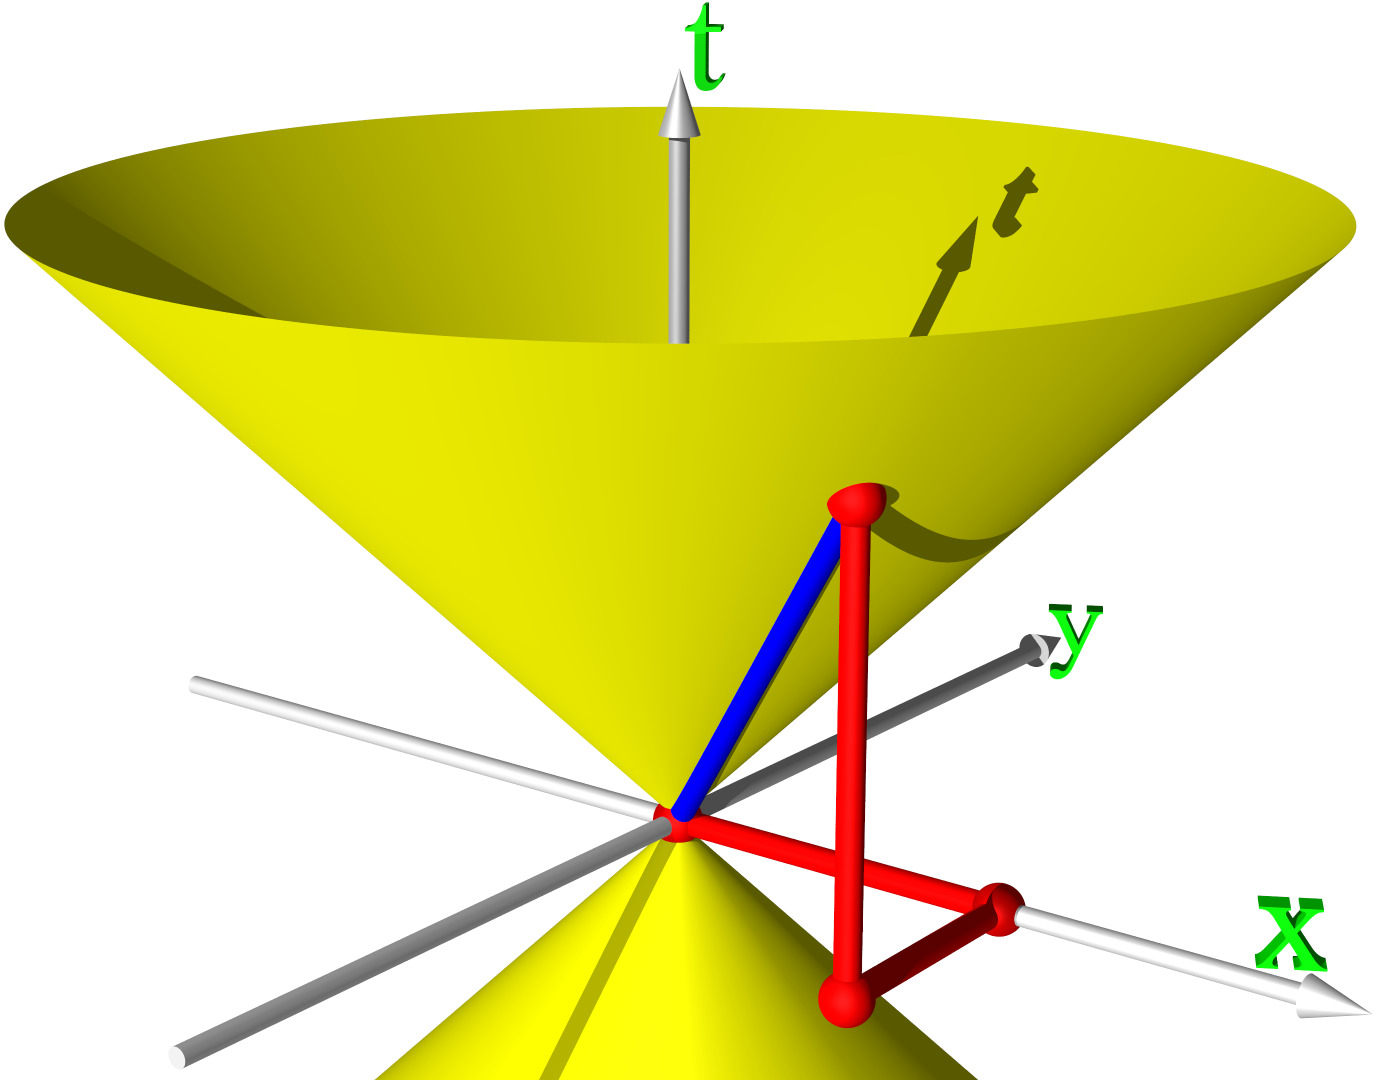
\includegraphics[width=\hsize]{chapters/3d/lichtkegel.jpg}
\caption{Lichtkegel ausgehend vom Nullpunkt zur Zeit $t=0$.
Alle Punkte innerhalb des Kegels mit $t>0$ liegen in der Zukunft des
Beobachters im Nullpunkt, solche mit $t<0$ in seiner Vergangenheit.
Punkte ausserhalb des Kegels können vom Nullpunkt aus nicht
beeinflusst werden.
Nur Punkte innerhalb des Kegels mit $t<0$ können Einfluss haben
auf den Nullpunkt.
\label{skript:kruemmung:fig:lichtkegel}}
\end{figure}

Das Vorzeichen des Ausdrucks~\eqref{skript:kruemmung:raumzeitabstand}
beschreibt also, ob zwei Ereignisse sich gegenseitig beeinflussen
können. 
Ist er negativ, dann ist eine Beeinflussung mit einer Wirkung möglich,
die sich weniger schnell als Licht ausbreitet.
Ist er gleich $0$, ist nur eine Beeinflussung mit einer Wirkung möglich,
die sich mit Lichtgeschwindigkeit ausbreitet.
Ist er positiv, ist keine gegenseitige Beeinflussung möglich.
Dies führt auf eine Unterteilung des Raumes in drei Gebiete
(Abbildung~\ref{skript:kruemmung:fig:lichtkegel}).
Die Fläche mit der Gleichung
\[
-c^2t^2+x^2+y^2+z^2=0
\]
heisst der Lichtkegel.
Ereignisse innerhalb des Lichtkegels mit $t>0$ können vom Nullpunkt aus
beeinflusst werden.
Ereignisse innerhalb des Lichtkegels imt $t<0$ können auf den Nullpunkt
Einfluss nehmen.
Alle anderen Ereignisse können den Nullpunkt weder beeinflussen
noch von ihm beeinflusst werden.
Sie müssen daher als die Gegenwart des Nullpunktes bezeichnet
werden.

In diesem Bild gibt es also keinen sinnvollen Begriff der Gleichzeitigkeit
mehr.
Wäre das Universum nicht aus einem Punkt entstanden, wie das Big Bang-Modell
besagt, dann wäre bereits die Frage ``Wann ist das Universum entstanden''
unsinnig, denn es gibt keinen sinnvollen Art und Weise, wie etwas gleichzeitig
im ganzen Universum stattfinden könnte.
Diese Beobachtung hat zu Einsteins Zeit aber keine grossen Wellen
geworfen, denn die meisten Phyisker gingen davon aus, dass das Universum
ewig und statisch ist, dass es also gar keinen Anfang braucht.
Auch Einstein ging davon aus, was ihn später in seiner allgemeinene
Relativitätstheorie dazu gebracht hat, einen nicht weiter erklärbaren
Term hinzuzufügen, einzig um zu erreichen, dass das Universum statisch 
sein kann.

\section{Lorentztransformation}
\rhead{Lorentztransformation}
Der Ausdruck~\eqref{skript:kruemmung:raumzeitabstand} ist nicht
invariant bei einer Galilei-Transformation.
Damit stellt sich die Frage, welche Transformationen denn
invariant wären.
Dies wären die Koordinaten-Änderungen, die zulässig sind, wenn
man das grundlegende Gesetz~\eqref{skript:kruemmung:raumzeitabstand}
der Kausalität erhalten will.

Zunächst sind Koordinatentransformationen, die nur die Raumkoordinaten
$x$, $y$ und $z$ beeinflussen, und den räumlichen Abstand nicht
ändern, zulässig.
Diese Transformationen sind aber wohlbekannt.
In der Linearen Algebra lernt man, dass genau die orthogonalen
Matrizen $A\in \textrm{O}(3)$, also Matrizen mit $A^tA=E$ diese
Eigenschaft haben.
Diese entsprechen räumlichen Drehungen und Spiegelungen.

Wenn sich aber zwei Koordinatensystem gegeneinander verschieben,
so wie bei der Galilei-Transformation, dann müssen auch die auch
die Zeitkoordinaten in die Transformation involviert sein.
Wir suchen also eine Koordinatentransformation, die nur die
$t$- und $x$-Koordinaten betrifft.
Wir können Sie in der Form
\begin{equation}
\begin{linsys}{3}
t'&=& a_{11}t&+&a_{12}x\\
x'&=& a_{21}t&+&a_{22}x
\end{linsys}
\end{equation}
ansetzen.
Wir verlangen jetzt aber, dass der
Ausdruck~\eqref{skript:kruemmung:raumzeitabstand}
unverändert bleibt.
Da die $y$- und $z$-Koordinaten ohnehin nicht involviert sind, bedeutet
das, dass
\begin{align*}
-c^2t^2 + x^2
&=
-c^2t'^2 + x'^2
\\
&=
-c^2(a_{11}t+a_{12}x)^2 + (a_{21}t+a_{22}x)^2
\\
&=
-c^2a_{11}^2t^2 -2c^2a_{11}a_{12}tx -c^2a_{12}^2x^2
+a_{21}^2t^2+2a_{21}a_{22}tx+a_{22}^2x^2
\\
&=
-(c^2a_{11}^2 - a_{21}^2)t^2
+2(-c^2a_{11}a_{12}+a_{21}a_{22})tx
+(-c^2a_{12}^2 + a_{22}^2)x^2
\end{align*}
Da dies für beliebige Werte von $x$ und $t$ gelten muss, müssen die
Koeffizienten der beiden Seiten übereinstimmen. 
Wir erhalten damit für die Koeffizienten $a_{ik}$ die Gleichungen
\[
\begin{aligned}
c^2a_{11}^2-a_{21}^2&=c^2
&&\Rightarrow&
a_{11}^2
-
\biggl(\frac{a_{21}}{c}\biggr)^2
&=1
\\
-c^2a_{12}^2+a_{22}^2&=1
&&\Rightarrow
&
a_{22}^2 - (ca_{12})^2&=1
\\
a_{21}a_{22}&=c^2a_{11}a_{12}
\end{aligned}
\]
Da die Differenz der Quadrate jeweils $1$ ist, können die Basen
als Werte des hyperbolischen Kosinus und Sinus dargestellt werden:
\[
\begin{aligned}
a_{11}&=\cosh\beta  &&&\frac{a_{21}}{c}&=\sinh\beta
\\
a_{22}&=\cosh\gamma &&&ca_{12}&=\sinh\gamma
\end{aligned}
\]
Die dritte Gleichung lautet dann
\begin{align*}
a_{21}a_{22}=c\sinh\beta\cosh\gamma
&=
c^2a_{11}a_{12}=c^2\cosh\beta\frac1c\sinh\gamma
\\
c\sinh\beta\cosh\gamma
&=
c\cosh\beta\sinh\gamma
\\
\tanh\beta&=\tanh\gamma,
\end{align*}
es folgt $\beta=\gamma$.
Damit haben wir die gesuchte Transformation gefunden, es ist
\begin{equation}
\begin{pmatrix}
a_{11}&a_{12}\\
a_{21}&a_{22}
\end{pmatrix}
=
\begin{pmatrix}
 \cosh\beta&\frac1c\sinh\beta\\
c\sinh\beta&\cosh\beta
\end{pmatrix}
\end{equation}
Um die physikalische Bedeutung des Parameters $\beta$ zu verstehen, 
betrachten wir die Punkte $x=0$ für beliebige $t$.
Sie werten abgebildet auf
\[
x' = c\sinh\beta t
\]
Im $(t',x')$-Koordinatensystem bewegt sich also der Nullpunkt des 
$(t,x)$-Koordinatensystems mit der Geschwindigkeit
\[
v=c\sinh\beta
\]
Der Parameter $\sinh\beta$ hat also die Bedeutung einer in Einheiten
der Lichtgeschwindigkeit gemessenen Geschwindigkeit.
Da also $v/c=\sinh\beta$ ist, kann man die Transformation auch
als
\begin{equation}
\begin{pmatrix}
a_{11}&a_{12}\\
a_{21}&a_{22}
\end{pmatrix}
=
\begin{pmatrix}
\displaystyle\sqrt{1-\biggl(\frac{v}{c}\biggr)^2}
	&\displaystyle\frac{v}{c^2} \\
v
	&\displaystyle\sqrt{1-\biggl(\frac{v}{c}\biggr)^2}
\end{pmatrix}
\label{skript:kruemmung:lorentz}
\end{equation}
schreiben.
Die Transformation 
\eqref{skript:kruemmung:lorentz}
heisst {\em Lorentz-Transformation}.
\index{Lorentz-Transformation}


\section{Energie und Impuls}
\rhead{Energie und Impuls}


%
% k-gravitatzion.tex
%
% (c) 2017 Prof Dr Andreas Müller, Hochschule Rapperswil
%
\chapter{Gravitation%
\label{skript:kruemmusng:sectipn:gravitation}}
\lhead{Gravitation}
\rhead{}
Albert Einstein hat erkannt, dass die Wirkung der Gravitation 
durch die Krümmung des Raumes beschrieben werden muss.
\index{Einstein, Albert}
In den folgenden Abschnitten geben wir einen Ausblick darauf, wie
die moderne Physik unseren Raum als einen gekrümmten Raum beschreibt.
An einfachen Modellen soll gezeigt werden, wie man sich die Gravitationswirkung
als die Wirkung eines gekrümmten Raumes vorstellen kann, wie schwarze Löcher
beschrieben werden können, und wie alle diese Dinge tatsächlich gemessen
werden können.

\section{Äquivalenzprinzip}
\rhead{Äquivalenzprinzip}
Schon Galileo Galilei hat bemerkt, dass im Gravitationsfeld der Erde
jeder Körper unabhängig von seiner Masse die gleiche Beschleunigung $g$
erfährt.
Auch das Newtonsche Gravitationsgesetz beschreibt den Betrag der Kraft
zwischen zwei Massen $M$ und $m$ als
\[
F=\frac{KMm}{r^2}.
\]
Ein Teilchen der Masse $m$ wird daher nach dem zweiten Newtonschen Gesetz
$F=ma$ immer mit den Betrag
\[
\frac{KM}{r^2}
\]
haben.
Die Beschleunigung eines Teilchens ist daher unabhängig von der Masse.
Diese {\em Äquivalenz\-prinzip} genannte Beobachtung wurde von
Lor\'and Eötvös 1909 mit sehr grosser Genauigkeit nachgemessen und bestätigt.
In neuerer Zeit wurde die Genauigkeit nochmals um den Faktor $10^4$
verbessert.

Eine Folge des Äquivalenzprinzips ist auch, dass sich ein konstant
beschleunigtes Labor und ein Labor in einem homogenen Gravitationsfeld
nicht unterscheiden lassen (Abbildung~\ref{skript:gravitation:labor}).
\begin{figure}
\centering
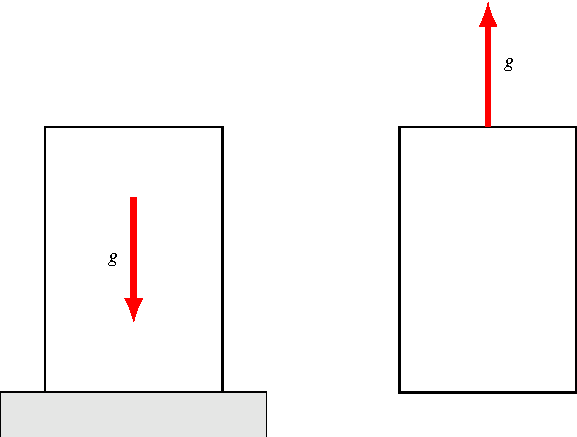
\includegraphics{chapters/tikz/labor.pdf}
\caption{Illustration des Äquivalenzprinzips.
Ein einem gleichmässig mit $g$ beschleunigten Labor (rechts)
misst man die gleiche Beschleunigung wie in einem homogenen
Gravitationsfeld (links).
\label{skript:gravitation:labor}}
\end{figure}
Ein beschleunigtes Koordinatensystem kann man zwar durch die
Koordinatentransformation
\begin{equation}
\left.
\begin{aligned}
t'&=t\\
x'&=x+\frac12gt^2
\end{aligned}
\right\}
\qquad
\Leftrightarrow
\qquad
\left\{
\begin{aligned}
t&=t'\\
x&=x'-\frac12gt'^2
\end{aligned}
\right.
\label{skript:gravitation:beschleunigt}
\end{equation}
erhalten, doch ist sie keine Lorentz-Transformation und erhält daher
die Minkowski-Metrik nicht.
Wenn es möglich sein soll, die Gravitationstheorie so zu verallgemeinern,
dass sie mit der speziellen Relativitätstheorie verträglich sein soll, dann
müssen wir auch andere Koordinatentransformationen als nur die
Lorenztransformation zulassen.
Das bedeutet aber, dass wir nicht mehr darauf beharren dürfen, dass
sich die Metrik in der Form
\begin{equation}
-c^2\,dt^2 + dx^2 + dy^2  + dz^2
\label{skript:gravitation:standardform}
\end{equation}
schreiben lässt.
Wir lassen daher in Zukunft beliebige Koordinatentransformationen zulassen
und daher auch Metriken $g_{\mu\nu}$, die von der
Standardform~\eqref{skript:gravitation:standardform} abweichen.

Wir wollen die Metrik berechnen, die im festen Koordinatensystem
anzuwenden ist. 
Dazu müssen wir die Transformation zuerst mit $x^0$ und $x'^0$ 
darzustellen:
\begin{equation}
\left.
\begin{aligned}
x'^0 &= x^0 \\
x'^1 &= x^1+\frac{1}{2c^2}(x^0)^2
\end{aligned}
\right\}
\qquad
\Leftrightarrow
\qquad
\left\{
\begin{aligned}
x^0 &= x'^0 \\
x^1 &= x'^1 - \frac{1}{2c^2}(x'^0)^2
\end{aligned}
\right.
\end{equation}
Für die Transformation der Metrik werden die partiellen Ableitungen
benötigt:
\begin{equation}
\begin{aligned}
\frac{\partial x^0}{\partial x'^0}&=1,
&
\frac{\partial x^0}{\partial x'^1}&=0,
&
\frac{\partial x^1}{\partial x'^0}&=-\frac{1}{c^2}x'^0,
&
\frac{\partial x^1}{\partial x'^1}&=1,
\\
\frac{\partial x'^0}{\partial x^0}&=1,
&
\frac{\partial x'^0}{\partial x^1}&=0,
&
\frac{\partial x'^1}{\partial x^0}&=\frac{1}{c^2}x^0,
&
\frac{\partial x'^1}{\partial x^1}&=1.
\end{aligned}
\end{equation}
Die zugehörige Transformationsmatrix ist also
\begin{equation}
\frac{\partial (x^0, x^1)}{\partial (x'^0, x'^1)}
=
\begin{pmatrix}
1&0\\
-\frac1{c^2}x'^0&1
\end{pmatrix},
\qquad
\frac{\partial (x'^0, x'^1)}{\partial (x^0, x^1)}
=
\begin{pmatrix}
1&0\\
\frac1{c^2}x^0&1
\end{pmatrix}.
\end{equation}
Im $(x^0,x^1)$-Koordinatensystem wird die Metrik durch die Matrix
\[
g_{\mu\nu}
=
\begin{pmatrix}-1&0\\0&1\end{pmatrix}
\]
ausgedrückt.
In $(x'^0,x'^1)$-Koordinaten muss die Matrix daher sein
\begin{align*}
g'_{\mu\nu}
&=
\begin{pmatrix}
1&0\\
\frac1{c^2}x'^0&1
\end{pmatrix}
\begin{pmatrix}
-1&0\\0&1
\end{pmatrix}
\begin{pmatrix}
1&\frac1{c^2}x'^0\\
0&1
\end{pmatrix}
=
\begin{pmatrix}
1&0\\
\frac1{c^2}x'^0&1
\end{pmatrix}
\begin{pmatrix}
-1&-\frac1{c^2}x'^0\\
 0& 1
\end{pmatrix}
\\
&=
\begin{pmatrix}
-1&-\frac1{c^2}x'^0\\
-\frac1{c^2}x'^0&1+\frac1{c^4}(x'^0)^2
\end{pmatrix}.
\end{align*}
Die Metrik $g'_{\mu\nu}$ ist offenbar wieder symmetrisch.
Wir könnten die Christoffelsymbole ausrechnen und die Geodäten
bestimmen, wir würden die Transformation von Geraden aus dem
$(x,t)$-Koordinatensystem finden.

\section{Newtonsche Gravitationstheorie%
\label{skript:section:newtonschegravitationstheorie}}
\rhead{Newtonsche Gravitationstheorie}
Als ersten Schritt in Richtung auf eine allgemeine Gravitationstheorie
zeigen wir, wie auch die Bahnen in einem Newtonschen Gravitationsfeld 
als Geodäten eines Zusammenhangs schreiben lassen.
Wer verwenden dazu aber nicht die Metrik und den daraus abgeleiteten 
Zusammenhang, dies hat erst die Einsteinsche Theorie geschafft.

\subsection{Schwerkraft}
Das Newtonsche Gravitationsgesetz beschreibt die Beschleunigung, die
auf ein Teilchen in einem Gravitationsfeld wirkt, welches von einer
Masse $m$ erzeugt wird.
Der Betrag der Kraft ist umgekehrt proportional zum Quadrat der
Entfernung.
Der Kraftvektor kann deshalb als
\begin{equation}
\vec F = -\frac{KM}{r^2}\cdot\frac{\vec r}{r}
\label{skript:gravitation:gkraft}
\end{equation}
geschrieben werden.
Die Bewegungsgleichung ist daher 
\begin{equation}
\ddot x^k = -\frac{KM}{r}\cdot\frac{x^k}{r},
\qquad\text{mit}\qquad r = \sqrt{(x^1)^2+(x^2)^2+(x^3)^2},
\label{skript:gravitation:bewegungsgleichung}
\end{equation}
es kommt nur die Beschleunigung und die Position vor.

In den Geodätengleichungen 
\[
\ddot x^\mu = -\Gamma^\mu_{\alpha\nu}\dot x^\alpha\dot x^\nu
\]
kommt dagegen auf der rechten Seite auch die Geschwindigkeit vor.
Es ist daher nicht unmittelbar klar, wie die Bewegungsgleichung als
Geodätengleichung geschrieben werden klar.

Wir beschreiben die Bewegung wieder in einem Vierdimensionalen Raum,
also als Kurve
\[
t\mapsto (t,x^1(t),x^2(t),x^3(t)),
\]
also mit $x^0(t)=t$.
Für eine solche Parametrisierung gilt $\dot x^0(t)=1$.
In der Geodätengleichung können wir daher die Terme mit mit Index $0$
separat behandelt werden:
\[
\ddot x^\mu
=
-\Gamma^\mu_{00}
-\Gamma^\mu_{k0}\dot x^k -\Gamma^\mu_{0l}\dot x^l
- \Gamma^\mu_{kl}\dot x^k\dot x^l
\]
Da in der Bewegungsgleichung~\eqref{skript:gravitation:bewegungsgleichung}
auf der rechten Seite keine Geschwindigkeiten vorkommen, darf nur der
erste Term stehen bleiben, also
\begin{equation}
\Gamma^k_{00} = \frac{KM}{r^2}\cdot \frac{x^k}{r},\qquad k=1,\dots,3.
\label{skript:gravitation:newtonzusammenhang}
\end{equation}
Da die erste Komponente der Geodäte $x^0(t)=t$ ist und seine zweite
Ableitung $\ddot x^0(t)=0$, muss auch $\Gamma^0_{\alpha\nu}=0$ sein.
Die einzigen nicht verschwindenden Zusammenhangskoeffizienten sind
\eqref{skript:gravitation:newtonzusammenhang}.

Man kann für den Zusammenhang~\eqref{skript:gravitation:newtonzusammenhang}
auch die Definition des Riemann-Krümmungstensors anwenden.
Die Rechnung zeigt aber, dass zwar einzelne Komponenten des Riemann-Tensors
nicht verschwinden, der Ricci-Tensor und damit auch der Einstein-Tensor
verschwinden dagegen identisch.
Diese Beschreibung der Gravitation führt also nicht auf das Modell
eines gekrümmten Raumes.

\subsection{Gravitationspotential}
Die potentielle Energie, die zur
Gravitationskraft~\eqref{skript:gravitation:gkraft} gehört, kann
mit Hilfe eines Wegintegrals berechnet werden.
Dazu verwenden wir einen Weg vom Punkt $P_1$ mit Radius $r_1$
zum Punkt $P_2$ mit Radius $r_2$ führt.
Da die Kraft immer radial wirkt, ist entlang des Weges nur die radiale
Komponente des Tangentialvektors massgebend.
Der Unterschied in der poteniellen Energie ist
\[
\Delta E
=
\int_{P_1}^{P_2} \vec F\cdot d\vec s
=
\int_{r_1}^{r_2} -\frac{KM}{r^2}\,dr
=
\biggl[
\frac{KM}{r}
\biggr]_{r_1}^{r_2}
=
GM\biggl(\frac{1}{r_2}-\frac{1}{r_1}\biggr).
\]
Legt man den Nullpunkt der potentiellen Energie ins unendliche, dann ist
das Potential einer Punktmasse mit Masse $M$ ist also
\begin{equation}
\varphi = \frac{KM}{r}.
\label{skript:gravitation:potential}
\end{equation}

Aus dem Potential kann man die Kraft mit Hilfe des Gradienten
berechnen.
Zur Berechnung brauchen wir die Ableitung von $r$ nach den Koordinaten.
Die Ableitung nach $x$ ist
\[
r=\sqrt{x^2+y^2+z^2}
\qquad\Rightarrow\qquad
\frac{\partial r}{\partial x}
=
\frac{1}{2r} \frac{\partial (x^2+y^2+z^2)}{\partial x}
=
\frac{1}{2r} 2x=\frac{x}{r}.
\]
Damit können wir jetzt die Ableitung des Potentials berechnen:
\begin{align*}
\frac{\partial}{\partial x}\frac1{r}
&=
-\frac{1}{r^2} \frac{\partial r}{\partial x}
=
-\frac{1}{r^2} \frac{x}{r}.
\end{align*}
Der Gradient
\[
\operatorname{grad}\varphi
=
-\frac{KM}{r^2}\cdot\frac1r\begin{pmatrix}x\\y\\z\end{pmatrix}
=
-\frac{KM}{r^2}\cdot\frac{\vec r}{r} = \vec F
\]
stimmt mit der Gravitationskraft überein.

Für eine ausgedehnte Masseverteilung mit Dichte $\varrho$ kann man das
Potential als Überlagerung von einzelnen Potentialen der
Form~\eqref{skript:gravitation:potential} berechnen.
%Das Integral
%\[
%\varphi(\vec r)
%=
%G\int_{\mathbb R^3} \frac{\varrho(\vec r')}{|\vec r-\vec r'|}\,d^3r',
%\]
%wobei das Integral als Volumen-Integral über alle Vektoren $\vec r'$
%zu erstrecken ist.
Eine solche Beschreibung
ist allerdings für unsere Zwecke nicht sehr nützlich.

Eine besser geeignete Beschreibung können wir aus dem Gausschen
Divergenzsatz erhalten.
Eine zweidimensionale Version dieses Satzes können wir
aus dem Satz von Green~\eqref{skript:kruemmung:satz:green}
erhalten.
Dazu verwenden wir die Funktionen 
\[
f(x)=-\frac{\partial \varphi}{\partial x}
\qquad\text{und}\qquad
g(x)=\frac{\partial \varphi}{\partial y}.
\]
Die linke Seite des Satzes von Green ist das Integral
\begin{equation}
\oint_{C}
\frac{\partial \varphi}{\partial x} \dot (-x(s))
\frac{\partial \varphi}{\partial y} \dot y(s)
\,ds
\label{skript:gravitation:fluss1}
\end{equation}
Der Vektor
\[
\vec o(s) = \begin{pmatrix}-\dot x(s)\\\dot y(s)\end{pmatrix}
\]
steht senkrecht auf dem Rand des Gebietes.
Im Integral~\eqref{skript:gravitation:fluss1} wird das Skalarprodukt
diese Vektors mit dem der Gravitationskraft $\vec F$ verwendet,
man nennt
\[
\oint_{C} \vec F\cdot \vec o(s)\,ds
\]
den Fluss des Vektorfeldes durch die Kurve $C$.
Auf der rechten Seite findet man dann 
\[
\int \frac{\partial g}{\partial x}-\frac{\partial f}{\partial x}\,dx\,dy
=
\int
\frac{\partial^2\varphi}{\partial x^2}
+
\frac{\partial^2\varphi}{\partial y^2}
\,dx\,dy
=
\int\Delta\varphi \,dx\,dy.
\]
Der Satz von Gauss besagt daher
\[
\oint_{C} \vec F\cdot d\vec o
=
\int_{D} \Delta\varphi\,dx\,dy.
\]
In dieser zweidimensionalen Darstellung nützt uns der Satz allerdings
wenig, denn das Gravitationsfeld ist natürlich dreidimensional.
Die dreidimensionale Version kann jedoch mit ganz ähnlichen Ideen
bewiesen werden wie der Satz von Green:

\begin{satz}[Gauss] Ist $\vec v$ ein Vektorfeld in
einem dreidimensionalen Gebiet $D\subset R^3$ mit Randfläche $S=\partial D$,
dann gilt
\begin{equation}
\oint_S \vec v\cdot d\vec o
=
\int_D 
\frac{\partial v_x}{\partial x}
+
\frac{\partial v_y}{\partial y}
+
\frac{\partial v_z}{\partial z}
\,dx\,dy\,dz
=
\int_D \operatorname{div}\vec v\,dx\,dy\,dz.
\label{skript:gravitation:gausssatz}
\end{equation}
Darin ist $\vec o$ ein Vektor ein nach aussen zeigender Vektor, der
senkrecht auf der Oberfläche des Gebietes steht.
\end{satz}

Der Nutzen dieses Satzes ist, dass man den Fluss des Schwerkraftfeldes
$\vec F$ einer Punktladung durch eine mit der Masse konzentrischen
Kugel auch direkt berechnen kann.
Dann hat nämlich $\vec F$ auf der Kugeloberfläche $S^2$ überall den gleichen
Betrag, und die Richtung ist immer senkrecht auf der Kugeloberfläche.
Das Skalarprodukt in~\eqref{skript:gravitation:gausssatz} ist daher
einfach ein Produkt der Beträge und das Integral bekommt man durch
Multiplikation mit der Kugeloberfläche:
\[
\oint_{S^2_r} \vec F\cdot d\vec o
=
4\pi r^2
\frac{KM}{r^2}
=
4\pi KM.
\]
Der Fluss des Gravitationsfeldes mit Potential $\varphi$ durch einen
sehr kleinen Ball $B_r$ mit Radius $r$ hat daher den Wert
\[
\int_{S^2_r}\vec F\cdot d\vec o
=
4\pi K\int_{B_r} \varrho\,dx\,dy\,dz.
\]
Andererseits kann man nach dem Satz von Gauss auch die rechte 
Seite berechnen:
\begin{align*}
\int_{B_r} 4\pi G\varrho\,dx\,dy\,dz
&=
\int_{B_r}
\frac{\partial F_x}{\partial x}+
\frac{\partial F_y}{\partial y}+
\frac{\partial F_z}{\partial z}
\,dx\,dy\,dz
=
\int_{B_r}
\frac{\partial^2\varphi}{\partial x^2}+
\frac{\partial^2\varphi}{\partial y^2}+
\frac{\partial^2\varphi}{\partial z^2}
\,dx\,dy\,dz
\\
&=
\int_{B_r} \Delta\varphi\,dx\,dy\,dz.
\label{skript:gravitation:poisson-integral}
\end{align*}
mit der Abkürzung
\begin{equation*}
\Delta \varphi
=
\frac{\partial^2\varphi}{\partial x^2}+
\frac{\partial^2\varphi}{\partial y^2}+
\frac{\partial^2\varphi}{\partial z^2},
\end{equation*}
dem Laplace-Operator.
Da dies für Kugeln an beliebigen Punkten mit beliebigen Radien 
gilt, müssen die Integranden in~\eqref{skript:gravitation:poisson-integral}
übereinstimmen.
Es folgt, dass das Gravitationspotential $\varphi$ die Gleichung
\begin{equation}
\Delta \varphi = 4\pi G\varrho
\label{skript:gravitation:potentialgleichung}
\end{equation}
erfüllen.
Diese Gleichung werden wir später dazu verwenden, die Verbindung zwischen
der newtonschen und der einsteinschen Gravitationstheorie herzustellen.

\section{Schwache Felder und die Metrik}
Für schache Gravitationsfelder hat die Newtonsche Theorie gute Dienste
geleistet. 
Wir gehen daher davon aus, dass eine neue, allgemeinere Theorie die
newtonsche Theorie als Grenzfall erhalten muss.
Es muss also möglich sein, die Gravitationskräfte, die wir im 
Abschnitt~\ref{skript:section:newtonschegravitationstheorie} bereits
mit Hilfe des Zusammenhangs, also den Koeffizienten $\Gamma^\alpha_{\mu\nu}$
beschrieben haben, auch aus einer Metrik zu gewinnen.
Die Zusammenhangskoeffizienten in
Abschnitt~\ref{skript:section:newtonschegravitationstheorie} waren nicht
die Christoffelsymbole einer Metrik.

Wir möchten jetzt eine Metrik finden, die einerseits möglichst nahe
an der Minkovski-Metrik ist, deren zugehörige Geodäten andererseits die
Bewegung in einem schwachen Gravitationsfeld korrekt wiedergibt.
Als Metrik verwenden wir daher
\[
g_{\mu\nu}=\eta_{\mu\nu} + h_{\mu\nu}.
\]
Der erste Summan ist $\eta_{\mu\nu}$, der die Minkovski-Metrik 
wiedergibt, der zweite beschreibt die Abweichung,
wobei wir annehmen, dass $h_{\mu\nu}$ sehr klein ist.
Die zugehörigen Christoffelsymbole sind mit einiger, vorzugsweise
maschineller Rechnung zu finden.
Aus der Beschreibung des newtonschen Gravitationsgesetzes können wir
ablesen, dass wir die klassisch beobachteten Kräfte in Gestalt
des Christoffelsymbols
\[
\Gamma^{k}_{00}
=
-\frac{1}{2(h_{kk} + 1)}\frac{\partial h_{00}}{\partial x^k}
\]
wiederfinden müssen.
Da $h_{kk}$ im Vergleich zu $1$ sehr klein soll, bleibt
\[
\Gamma^{k}_{00}
=
-\frac{1}{2}\frac{\partial h_{00}}{\partial x^k}.
\]
Damit die Bahnen der newtonschen Gravitationstheorie entstehen, müssen
die $-\Gamma^k_{00}$ die Beschleunigungskomponenten des Gravitationsfelds
entstehen.
Diese bilden den Gradienten des Potentials des Gravitationsfeldes
\[
-\Gamma^k_{00} = -\frac{\partial\varphi}{\partial x^k}.
\]
Es folgt daher, dass $h_{00}=-2\varphi/c^2$ ist.
In erster Näherung beschreibt daher die Metrik
\begin{equation}
\begin{aligned}
g_{00} &= -1 -\frac{2\varphi}{c^2},
&&&
g_{kk} &= 1,\quad k=1,2,3.
\end{aligned}
\label{skript:gravitation:naeherung}
\end{equation}
Die gesuchte Theorie muss also in erster Näherung das newtonsche
Gravitationspotential in der $00$-Komponente des metrischen Tensors
verwenden.

\section{Einstein-Gleichungen für das Gravitationsfeld}
Die Näherung für schwache Felder dient uns nun als Leitfaden, um die
Einsteinschen Feldgleichungen herzleiten.
Einerseits beinhaltet die $g_{00}$-Komponente das Potential $\varphi$ des
Gravitationsfeldes, andererseits beschreibt die
Gleichung~\eqref{skript:gravitation:potentialgleichung}
den Zusammenhang zwischen dem Gravitationspotential und der
Masseverteilung.
Wir suchen jetzt eine Theorie, welche auch die übrigen Komponenten
des metrischen Tensors zu bestimmen erlaubt.
Wir gehen dazu mit Hilfe von Analogien vor, eine strenge Herleitung
der Gleichungen ist ebenfalls möglich, jedoch für dieses Skript etwas
zu aufwendig.

Für die folgenden mathematischen Objekte suchen wir einen Ersatz:
\begin{enumerate}
\item
Die Massedichte in 
Gleichung~\eqref{skript:gravitation:potentialgleichung}
muss durch eine Grösse ersetzt werden, die dem vorhandenen Vierer-Impuls
ebenfalls Rechnung trägt.
Ausserdem soll sie auch um andere Formen von Energie ergänzt werden 
können, um zum Beispiel die Gravitationswirkung der Energie eines
elektromagnetischen Feldes modellieren zu können.
\item
In Gleichung~\eqref{skript:gravitation:potentialgleichung}
kommen die zweiten Ableitungen nach den Koordinaten vor. 
Der Laplace-Operator lässt sich aber nur in der Minkowski-Metrik so 
formulieren, ausserdem trägt er der Zeitkoordinate nicht Rechnung.
Wir brauchen daher eine Grösse, die alle Koordinaten gleichwertig
behandelt, aber im Grenzfall schwacher Felder wieder auf den 
Laplace-Operator führt.
\item
Der Energieerhaltungssatz in Form der
Gleichung~\eqref{skript:speziell:energieerhaltung}
kann nicht aufrechterhalten werden, weil
Gravitationsfelder die Energie darin sich bewegender Massen verändern
können.
Es muss also eine Formulierung des Energie- und Impulserhaltungssatzes
gefunden werden, welche mit der erweiterten Theorie verträglich ist.
\end{enumerate}
Dieses Programm soll in den folgenden Abschnitten durchgeführt werden.
Am Ende soll in Analogie zur 
Potentialgleichung~\eqref{skript:gravitation:potentialgleichung}
eine Gleichung der Form
\[
\text{``Tensor zur Feldbeschreibung''}
=
4\pi K\cdot \text{``Tensor mit Energie und Impuls''}
\]
das Gravitationsfeld beschreiben.

\subsection{Massedichte und Energie-Impuls-Tensor}
Die Massedichte $\varrho$, die wir auf der rechten Seite der
Potentialgleichung~\eqref{skript:gravitation:potentialgleichung}
für das newtonsche Gravitationsfeld finden,
finden wir in der allgemeinen Theorie als $00$-Komponente
des Energie-Impuls-Tensors wieder.
Es ist daher naheliegend, dass auf der rechten Seite der gesuchten
Gleichung der Energie-Impuls-Tensor $T_{\mu\nu}$ stehen soll.

\subsection{Ricci- und Einstein-Tensor}
Auf der linken Seite der Gleichung erwarten wir ein Objekt, welches
sich aus den zweiten Ableitungen der $g_{\mu\nu}$ berechnen lässt.
Die Christoffel-Symbole enthalten die ersten Ableitungen von $g_{\mu\nu}$,
aber der Riemannsche Krümmungstensor enthält alle zweiten Ableitungen.
Wir müssen daher einen Tensor $G_{\mu\nu}$ konstruieren, der die Rolle
von $\Delta\varphi$ übernehmen kann.
In Analogie zur
Gleichung~\eqref{skript:gravitation:potentialgleichung}
erwarten wir dann eine Gleichung der Form
\[
G^{\mu\nu} = 4\pi KT^{\mu\nu}
\]
als allgemeine Feldgleichung für die Gravitation.

Der Riemann-Tensor $R^\mu\mathstrut_{\nu\varrho\sigma}$ hat zu viele
Indizes, es muss daraus erst ein Tensor zweiter Stufe hergestellt werden.
Dies ist zum Beispiel durch Verjüngung möglich.
Wegen der Symmetrieeigenschaften des Riemann-Tensors gibt es nicht allzuviele
Möglichkeiten, wie dies geschehen könnte.
Die Verjüngung 
\[
R_{\mu\nu} = R^{\alpha}\mathstrut_{\mu\alpha\nu}
\]
heisst der Ricci-Tensor.
Wegen
\[
R_{\mu\nu}
=
R^{\alpha}\mathstrut_{\mu\alpha\nu}
=
R^{\alpha}\mathstrut_{\nu\alpha\mu}
=
R_{\nu\mu}
\]
ist er symmetrisch.

Diesen kann man weiter verjüngen und daraus den Krümmungs-Skalar
\[
R=R^\alpha\mathstrut_\alpha
\]
bilden.
Den gesuchten Tensor $G_{\mu\nu}$ können wir als Linearkombination
\[
G_{\mu\nu}=a R_{\mu\nu} + bg_{\mu\nu} R
\]
ansetzen.
Der Krümmungsskalar $R$ ist eine Invariante, wir brauchen den Faktor
$g_{\mu\nu}$, um daraus einen Tensor zu machen, der mit dem Ricci-Tensor
$R_{\mu\nu}$ linear kombiniert werden kann.
Die Koeffizienten $a$ und $b$ sind noch zu bestimmen.

\subsection{Energieerhaltung und Feldgleichungen}
Der Energie-Impuls-Tensor der speziellen Relativitätstheorie
% XXX Referenz
erfüllt den Erhaltungssatz
\[
\frac{\partial T^\mu_\nu}{\partial x^\mu}
=0.
\]
Wir können allerdings nicht annehmen, dass diese Formel weiterhin
gelten wird.
Das Gravitationsfeld kann ja zum Beispiel ein Gas beschleunigen und 
verdichten, so dass sich Energie- und Impuls-Inhalt verändern können.
Dies können durch die kovariante Ableitung
\[
0
=
\nabla_\mu T^\mu_\nu
=
\frac{\partial T^\mu_\nu}{\partial x^\mu}
-
\Gamma^{\mu}_{\alpha\mu}T^\alpha_\nu
\]
ausdrücken.
Die Terme mit den Christoffel-Symbolen zeigen, wie die Gravitationskraft
Energie und Impuls verändert.




%
% k-schwarzschild.tex
%
% (c) 2017 Prof Dr Andreas Müller, Hochschule Rapperswil
%
\chapter{Schwarzschild-Metrik und schwarze Löcher%
\label{skript:chapter:schwarzschild}}
\lhead{Schwarzschild-Metrik}
\rhead{}
Die Einsteinschen Feldgleichungen schränken die Metriken ein,
die in einem Raumzeit-Gebiet über\-haupt möglich sind.
Damit stellt sich automatisch die Frage, wie die Einsteinsche Theorie 
das Gravitationsfeld in der Umgegung eines Sterns beschreiben kann.
Schon wenige Monate nachdem Einstein seine allgemeine Relativitätstheorie
veröffentlich hat, hat Karl Schwarzschild eine Lösung der Einsteinschen
Feldgleichungen gefunden.
Daraus lassen sich die Bewegungsgleichungen eines Körpers in der Nähe
eines Sterns ableiten und es sollte möglich sein, den Unterschied zwischen
der Newtonschen Gravitations-Theorie und Einsteinschen  zu quantifizieren
und damit Tests der allgmeinen Relativitätstheorie zu ermöglichen.

\section{Eine kugelsymmetrische, statische Lösung}
\rhead{Schwarzschild-Metrik}
Karl Schwarzschild suchte eine Metrik, die sich mit der Zeit nicht ändert,
also
\[
\frac{\partial g_{\mu\nu}}{\partial t}=0,
\]
und die ausserdem kugelsymmetrisch sein soll.
Diese Metrik sollte eine erste Approximation für die Gravitation in
der Umgebung eines Sterns sein.
Natürlich berücksichtigt dieses Modell weder, dass sich Sterne mit
der Zeit entwickeln, noch die Tatsache, dass sich Sterne normalerweise
um eine Achse drehen, dass man also gar nicht eine rotationssymmetrische
Lösung erwarten darf.

Die Längenmessung
\begin{equation}
ds^2
=
-c^2\,dt^2 + dr^2 + r^2 d\Omega^2
\qquad
d\Omega^2 = d\vartheta^2 + \sin^2\vartheta\,d\varphi^2
\label{skript:kruemmung:euklid}
\end{equation}
im Raum mit Kugelkoordinaten ist natürlich eine solche Metrik,
doch da dies nur eine andere Parametrisierung des euklidischen
Raumes ist, ist diese Geometrie flach.
Sie kann also sich nicht ein Modell eines Sternes sein.

Man kann eine Lösung der Feldgleichungen finden, indem man den
einzelnen Termen der euklischen Metrik~\eqref{skript:kruemmung:euklid}
zunächst unbestimmte Faktoren hinzufügt, die nur von $r$ abhängt,
und dann mit Hilfe der Feldgleichungen dafür Differentialgleichungen
herleitet.
Wir wollen diesen beschwerlichen Weg nicht gehen, und uns mit dem
Resultate zufriedenstellen, es lautet
\begin{equation}
ds^2
=
-\biggl(1-\frac{r_g}r\biggr)c^2\,dt^2
+\frac1{\displaystyle 1-\frac{r_g}r}\,dr^2 + r^2\,d\Omega^2.
\label{skript:kruemmung:schwarzschildmetrik}
\end{equation}
Man kann nachrechnen, zum Beispiel mit Hilfe der früher vorgestellen
Maxima-Programme, dass der Einstein-Tensor für diese Metrik überall
verschwindet.

\section{Der Fall $r=r_g$}
\rhead{Der Fall $r=r_g$}
Es scheint, dass die Metrik für $r=r_g$ nicht wohldefiniert ist,
da dann der Nenner im zweiten Term nicht wohldefiniert ist.
Dem ist jedoch nicht so, wie man durch Wahl eines anderen Koordinatensystems
zeigen kann.
Wir ersetzen die Zeitkoordinaten $t$ durch $\tau$, und die $r$-Koordinate
durch $R$ mit der vorläufig noch unbestimmten Funktion $f(r)$.
Es soll gelten
\begin{equation}
\begin{aligned}
c\tau
&=
ct + \int\frac{f(r)\,dr}{\displaystyle 1-\frac{r_g}{r}}
&
&\text{und}
&
R
&=
ct
+
\int\frac{dr}{\displaystyle \biggl(1-\frac{r_g}{r}\biggr)f(r)}
\end{aligned}
\label{skript:kruemmung:finkelsteindefinition}
\end{equation}
mit einer vorläufig noch unbestimmten Funktion $f(r)$.
Die Integrationskonstante in den beiden unbestimmten Integralen
entspricht einer Wahl des $t$- bzw.~$\tau$-Nullpunktes und ist
daher nicht von Bedeutung.
Um die Metrik in $\tau$ und $R$ ausdrücken zu können, müssen wir 
den Zusammenhang zwischen $dr$, $dR$, $dt$ und $d\tau$ kennen.
Wir finden diesen durch Ableiten der beiden Definitionsgleichungen
\eqref{skript:kruemmung:finkelsteindefinition}:
\begin{align*}
c\,d\tau
&=
c\,dt + \frac{f(r)}{\displaystyle 1-\frac{r_g}{r}}\,dr,
\\
dR
&=
c\,dt
+
\frac{1}{\displaystyle\biggl(1-\frac{r_g}{r}\biggr)f(r)}\,dr.
\end{align*}
Für die Schwarzschild-Metrik brauchen wir die Quadrate davon:
\begin{align*}
c^2\,d\tau ^2
&=
c^2\,dt^2 + 2\frac{cf(r)}{\displaystyle 1-\frac{r_g}{r}}\,dt\,dr
+\frac{f(r)^2}{\biggl(\displaystyle 1-\frac{r_g}{r}\biggr)^2}\,dr^2,
\\
dR^2
&=
c^2\,dt^2 + 2\frac{c}{\displaystyle\biggl(1-\frac{r_g}{r}\biggr)f(r)}\,dt\,dr
+
\frac{1}{\displaystyle \biggl(1-\frac{r_g}{r}\biggr)^2f(r)^2}\,dr^2.
\end{align*}
Wir müssen diese beiden Ausdrücke so kombinieren, dass der gemischte
Term $dt\,dr$ wegfällt, denn dieser kommt in der Schwarzschild-Metrik
nicht vor.
Dazu multiplizieren wir die zweite Zeile mit $f(r)^2$, und subtrahieren.
Wir erhalten
\begin{equation}
c^2\,d\tau^2 - f(r)^2\,dR^2
=
(1-f(r)^2)c^2\,dt^2
+\frac{f(r)^2-1}{\displaystyle\biggl(1-\frac{r_g}{r}\biggr)^2}\,dr^2.
\end{equation}
Damit daraus die Schwarzschild-Metrik wird, müssen wir vor dem $dt^2$
Term einen Faktor der Form $(1-r_g/r)$ haben, wir müssen also zunächst
alles durch $1-f(r)^2$ dividieren, und dann mit $1-r_g/r$ multiplizieren.
Wir kehren ausserdem das Vorzeichen und erhalten
\[
\frac{\displaystyle 1-\frac{r_g}{r}}{1-f(r)^2}
(-c^2\,d\tau^2 + f(r)^2\,dR^2)
=
-\biggl(1-\frac{r_g}{r}\biggr)c^2\,dt^2
+\frac{1}{\displaystyle 1-\frac{r_g}{r}}\,dr^2
\]
Bis auf die Terme $d\Omega^2$ steht auf der rechten Seite die
Schwarzschild-Metrik.
Von den Termen auf der linken Seite ist nur der Bruch
\[
\frac{\displaystyle 1-\frac{r_g}{r}}{1-f(r)^2}
\]
problematisch, allerdings nur, wenn der Nenner $1-f(r)^2$ eine
Nullstelle hat.
Wir können den ganzen Bruch zum Verschwinden bringen, indem wir die
Wahlmöglichkeiten für $f(r)$ ausnützen und 
\[
f(r)=\sqrt{\frac{r_g}{r}}
\]
wählen.
Setzen wir dies ein, erhalten wir die Metrik in $\tau$-$R$-Koordinaten
jetzt in der Form
\begin{equation}
ds^2
=
-c^2\,d\tau^2 + \frac{r_g}{r}\,dR^2 + r^2 d\Omega^2,
\label{skript:kruemmung:finkelstein}
\end{equation}
aber natürlich müssen wir $r$ und $r^2$ ebenfalls durch die Koordinaten
$\tau$ und $R$ ausdrücken.

Da jetzt $f(r)$ bekannt ist, können wir die
Integrale~\eqref{skript:kruemmung:finkelsteindefinition} auswerten.
Wir berechnen
\begin{align*}
R-c\tau
&=
\int\frac{dr}{\displaystyle \biggl(1-\frac{r_g}{r}\biggr)f(r)}
- \int\frac{f(r)\,dr}{\displaystyle 1-\frac{r_g}{r}}
=
\int\frac{1-f(r)^2}{\displaystyle\biggl(1-\frac{r_g}{r}\biggr) f(r)}\,dr
=
\int\frac{1}{f(r)}\,dr
=
\frac{1}{\sqrt{\mathstrut r_g}}\int\sqrt{\mathstrut r}\,dr
\\
&=
\frac{1}{\sqrt{\mathstrut r_g}} \frac{2}{3}r^{\frac{3}{2}}
\end{align*}
Damit kann man jetzt $r$ durch $R-c\tau$ ausdrücken
\begin{equation}
r
=
\biggl(\frac{3}{2}(R-c\tau)r_g^{\frac{1}{2}}\biggr)^{\frac23}
=
\biggl(\frac{3}{2}(R-c\tau)\biggr)^{\frac23} r_g^{\frac13}
\label{skript:kruemmung:finkelsteinr}
\end{equation}
Der $r$-Koordinate $r_g$ entspricht jetzt die Gerade
\[
R-c\tau = \frac23 r_g = R_g.
\]
Setzen wir dies in die Metrik~\eqref{skript:kruemmung:finkelstein}
ein, erhalten wir
\[
ds^2
=
-c^2 \,d\tau^2
+r_g^{\frac23}\biggl(\frac32(R-c\tau)\biggr)^{-\frac23}\,dR^2
+ r_g^{\frac23}\biggl(\frac32(R-c\tau)\biggr)^{\frac43}\,d\Omega^2.
\]
Es ist klar, dass in diesen Koordinaten in keinem Term für $r=r_g$
eine Singularität auftritt.
Die hier berechneten Koordinaten $\tau$ und $R$ heissen
Finkelstein-Koordinaten.

\section{Absturz ins Zentrum}
\rhead{Absturz ins Zentrum}
\begin{figure}
\centering
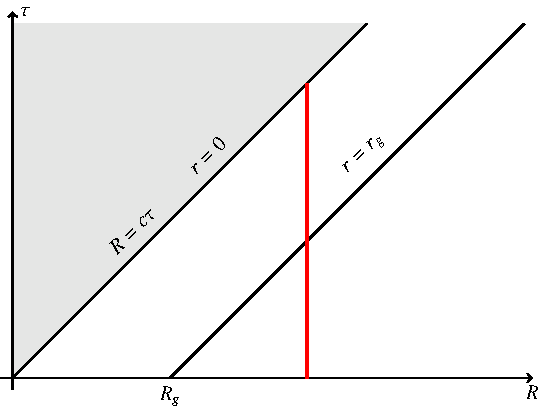
\includegraphics{chapters/tikz/absturz.pdf}
\caption{Radialer Absturz eines Teilchens (rote Bahn) in einem Zentralfeld
in Finkelstein-Koordinaten.
Das Teilchen stürzt in endlicher Eigenzeit ins Zentrum.
\label{skript:kruemmung:fig:absturz}}
\end{figure}
\begin{figure}
\centering
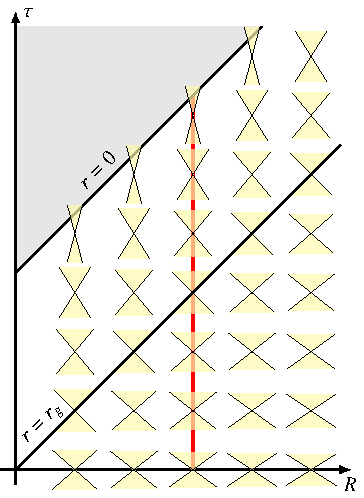
\includegraphics{chapters/tikz/lichtkegel.pdf}
\caption{Lichtkegel in Finkelstein-Koordinaten.
\label{skript:kruemmung:fig:lichtkegel}}
\end{figure}
In Finkelstein-Koordinaten verschwindet die Singularität bei $r=r_g$,
es sollte daher auch einfacher werden, die Bahn eines radial ins
Zentrum des Feldes stürzenden Teilchens zu berechnen.
Dazu können wir die Winkel-Koordinaten $\vartheta$ und $\varphi$
vernachlässigen, und nur mit den Koordinaten $\tau$ und $R$ und der
Metrik
\[
ds^2
=
-c^2 \,d\tau^2
+r _g^{\frac23}\biggl(\frac32(R-c\tau)\biggr)^{\frac23}\,dR^2
\]
arbeiten.
Zur Berechnung der Bahnkurven brauchen wir die Christoffel-Symbole
2.~Art.
Die Berechnung mit Maxima ergibt
\begin{align*}
\Gamma^1_{11} &= 0,&
\Gamma^1_{12} &= 0,&
\Gamma^1_{21} &= 0,&
\Gamma^1_{22} &= \frac{2^{\frac23}r_g^{\frac23}}{(3(R-c\tau))^{\frac53}},\\
\Gamma^2_{11} &= 0,&
\Gamma^2_{12} &= \frac1{3(R-c\tau)},&
\Gamma^2_{21} &= \frac1{3(R-c\tau)},&
\Gamma^2_{22} &= -\frac1{3(R-c\tau)}.
\end{align*}
Wir beschreiben die Bahn eines Teilchens welches sich in diesem Feld
radial bewegt mit den Funktionen $\tau(s)$ und $R(s)$.
Wir untersuchen ein Teilchen, welches beim Punkt $\tau(0)=0$ und $R(0)=R_0$
mit Anfangsrichtung $\dot\tau(0)=1$ und $\dot R(0)=0$ in das Gravitationsfeld
stürzt.
Die Geodätengleichungen lauten
\begin{align*}
\frac{d^2\tau(s)}{ds^2}
&=
\Gamma^1_{22}\biggl(\frac{dR(s)}{ds}\biggr)^2,
\\
\frac{d^2R(s)}{ds^2}
&=
\Gamma^2_{12}\frac{d\tau(s)}{ds}\frac{dR(s)}{ds}
+
\Gamma^2_{22}\biggl(\frac{dR(s)}{ds}\biggr)^2.
\end{align*}
Da für die Anfangsbedinung $\dot R=0$ ist und auf der rechten Seite
$\dot R$ in jedem Term vorkommt, folgt aus der zweiten Gleichung
$\ddot R=0$, $\dot R$ kann sich also nicht ändern.
Wenn aber $\dot R=0$ für alle Werte von $s$, dann ist nach der ersten
Gleichung auch $\ddot \tau=0$ und damit $\dot \tau=1$.
Die Lösungskurve ist also $R=R_0$ und $\tau=s$, rot dargestellt in
Abbildung~\ref{skript:kruemmung:fig:absturz}.

Mit Hilfe der Formel~\eqref{skript:kruemmung:finkelsteinr}
kann man damit auch $r$ für den radialen Absturz angeben:
\[
r(\tau)=\biggl(\frac32(R_0-c\tau)\biggr)^{\frac23}r_g^{\frac13}.
\]

\section{Ereignishorizont%
\label{skript:section:ereignishorizont}}
\rhead{Ereignishorizont}
Wir betrachten wieder die
Schwarzschild-Metrik~\eqref{skript:kruemmung:schwarzschildmetrik}
und möchten genauer verstehen, was bei $r=r_g$ passiert.
Dazu überlegen wir uns, wie ein Geodäte eines realen Teilchens 
aussieht.
Wir wissen, dass reale Teilchen sich so bewegen müssen, dass der
Tangentialvektor negative Metrik hat.
Ein Teilchen in Ruhe hat zum Beispiel $\dot r=0$, $\dot \vartheta=0$ und
$\dot varphi=0$, einzig $\dot t\ne 0$.
Da der Koeffizient von $dt^2$
\[
-\biggl(1-\frac{r_g}{r}\biggr)
\quad
\begin{cases}
<0&\qquad r > r_g
\\
>0&\qquad r < r_g
\end{cases}
\]
für $r>r_g$
negativ ist folgt, dass es tatsächlich möglich ist, dass sich ein Teilchen
in festem Abstand vom Zentrum aufhalten kann.
Sobald aber $r<r_g$ ist, ist der Koeffizient von $dt^2$ positiv,
fester Abstand vom Zentrum ist nicht mehr möglich.

Für $r<r_g$ wechselt aber auch das Vorzeichen des Koeffizienten
\[
\frac1{\displaystyle1-\frac{r_g}{r}}
\quad
\begin{cases}
>0&\qquad r>r_g
\\
<0&\qquad r<r_g
\end{cases}
\]
von $dr^2$, damit wird plötzlich der Vektor $\dot t=0$, $\dot r\ne 0$,
$\dot\vartheta=\dot\varphi=0$ zeitartig.
Sobald ein Teilchen sich innerhalb des Radius $r_g$ befindet, kann
sein Radius nur noch abnehmen.
Die Berechnung der Bahn eines solchen Teilchens zeigt auch, dass
es unausweichlich in endlicher Zeit ins Zentrum stürzen wird.

\begin{figure}
\centering
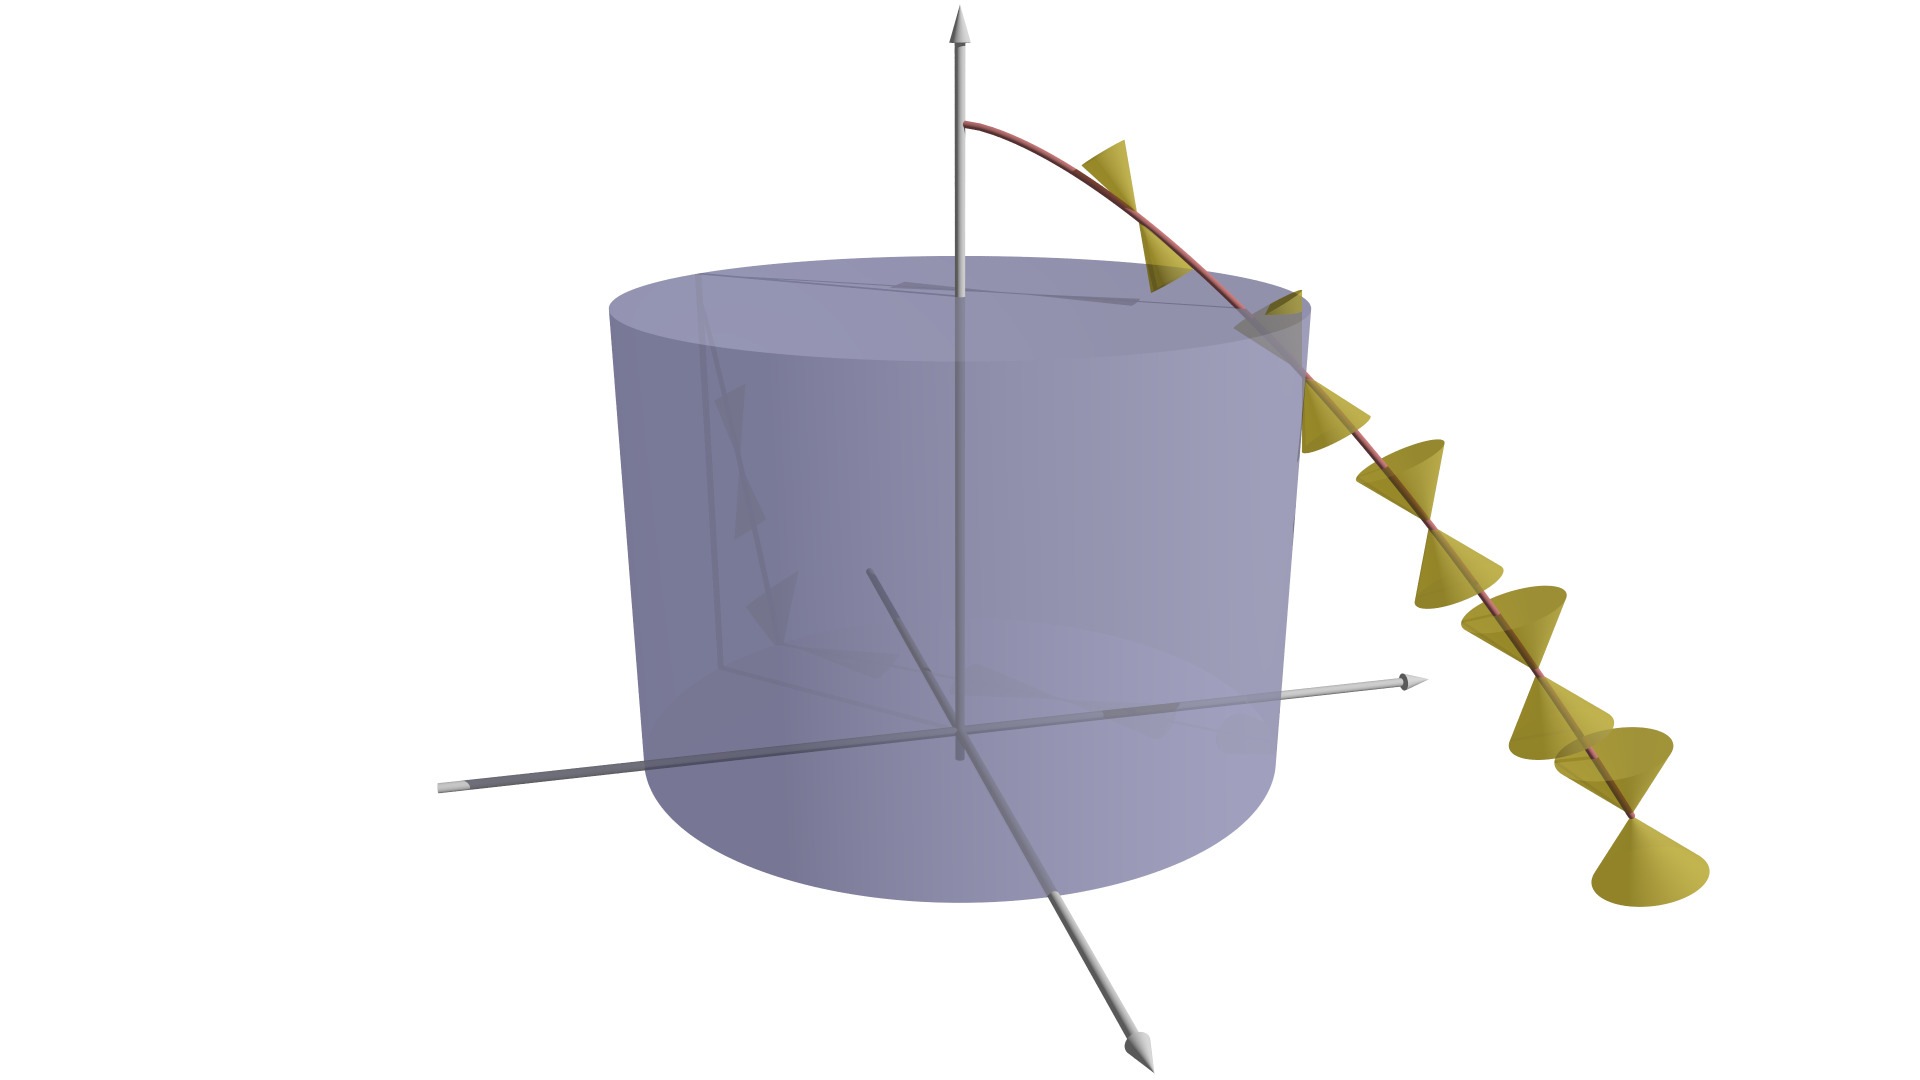
\includegraphics[width=\hsize]{chapters/3d/blackhole.jpg}
\caption{Absturz eines Teilchens durch den Ereignishorizont in
$(\tau,r,\varphi)$-Koordinaten.
Sobald das Teilchen durch den Ereignishorizont gefallen ist,
befindet sich der ganze zukünftige Lichtkegel eines Teilchens 
immer vollständig im inneren des Gebietes $r<r_g$.
\label{skript:kruemmung:fig:blackhole}}
\end{figure}


\section{Was spürt man am Ereignishorizont?%
\label{skript:section:wasspuertman}}
\rhead{Was spürt man am Ereignishorizont?}
Der Riemannsche Krümmungstensor gibt an, wie schnell Geodäten von Teilchen
wegen unterschiedlicher Gravitationswirkung sich voneinander entfernen.
Er bestimmt also die Gezeitenkräfte, die ein Astronaut spürt, der in
diesem Gravitationsfeld abstürzt.
die Gezeitenkräfte, die ein Astronaut spürt, der in
diesem Gravitationsfeld abstürzt.
Die Berechnung des Riemann-Tensors mit Maxima ergibt aber:
\begin{align*}
R_{1212}&=-\frac{r_g}{r^3},
\end{align*}
die Gezeitenkräfte in radialer Richtung werden für den Astronauten
also zwar immer grösser, aber bei $r=r_g$ spürt er nichts besonderes.

\section{Bedeutung von $r_g$}
\rhead{Bedeutung von $r_g$}
In Abschnitt~\ref{skript:section:ereignishorizont} haben wir gefunden,
dass sich bei der Koordinaten $r=r_g$ der Ereignishorizont befindet.
Es ist auch einigermassen klar, dass dieser Radius $r_g$ mit der
Masse des Objektes zusammenhängen muss.
Doch wie gross ist eiegentlich der Gravitations-Radius $r_g$ verschiedener
uns umgebender Himmelskörper? Kann es überhaupt einen Körper geben, der
so dicht ist, dass er kleiner ist als sein Gravitationsradius?


%
% robertson.tex -- Robertson Walker Metrik
%
% (c) 2017 Prof Dr Andreas Müller, Hochschule Rapperswil
%
\chapter{Kosmologie%
\label{skript:chapter:kosmologie}}
\lhead{Kosmologie}
\rhead{}
Die Einstein-Gleichungen ermöglichen erstmals, die Entwicklung
des ganzen Universums zu modellieren.
Dazu sind allerdings die Kenntnis der grossräumigen
Masseverteilung notwendig.
Es stellt sich heraus, dass diese im grossen isotrop und homogen ist.
Dies bedeutet, dass auch die Krümmung im Universum homogen und isotrop
ist.
Die Robertson-Walker-Metrik erfüllt diese Voraussetzung.

\section{Expansion des Universums}
\rhead{Expansion}
Zu Beginn des 20.~Jahrhunderts hatte man noch keine klare Vorstellung
über die Grösse des Universums.
Allgemein wurde angenommen, dass unsere Milchstrasse im wesentlichen das
ganze Universum ist.
Die seit längerer Zeit bekannten Nebel wurden als Teil der Milchstrasse
angesehen.
Auch wurde das Universum im wesentlichen als unveränderlich angesehen.

In den frühen zwanziger Jahren des 20.~Jahrhunderts gelang es dann
Edwin Hubble, die Entfernung von Andromeda und anderen heute als
Galaxien bekannten Nebeln zu bestimmen.
Er verwendete dafür sogenannte Cepheiden-Veränderliche.
Zwischen der absoluten Helligkeit dieser veränderlichen
Sterne und der Periode der Helligkeitsschwankungen besteht
eine einfache Beziehung.
Hubble fand Cepheiden-Veränderliche in Aufnahmen der Andromeda-Galaxie
und war damit in der Lage, deren absolute Helligkeit zu bestimmen.
Aus der beobachteten Helligkeit konnte er die Entfernung ableiten.
Es zeigte sich, dass diese Galaxien weit ausserhalb unserer Milchstrasse
befinden.

Hubble und sein Assistent Milton Humason massen mit dem neuen
2.5m-Hooker-Teleskop neben der Entfernung auch die Spektren und
damit die Rotverschiebung von 46 Galaxien.
Es zeigte sich, dass sich weiter entfernte Galaxien schneller 
entfernen.
Sie schlossen daraus, dass das Universum expandieren muss, sie konnten
sogar die Geschwindigkeit bestimmen, mit der dies geschieht.

Der belgische Physiker
Georges Lemaître hatte auf der Basis von Einsteins allgemeiner
Relativitätstheorie die Expansion des Universums bereits vor
Hubbles Entdeckung vorhergesagt.
Doch erst mit die Messungen von Hubble und Humason haben bewiesen,
dass Einsteins Theorie die Entwicklung des Universums korrekt
vorhersagen kann.

\subsection{Der Skalenfaktor}
Hubbles Beobachtungen haben gezeigt, dass sich das Universum ausdehnt.
Zwei nahe Punkte befinden sich zur Zeit $t_0$ in einem Abstand $d_0$,
und sollen in einem geeigneten Koordinatensystem in Ruhe sein.
Zu einer späteren Zeit wird die Distanz sich vergrössert haben.
Da das Universum isotrop und homogen ist, muss die Distanz in jeder
beliebigen Richtung um den gleichen Faktor gewachsen sein.
Die Ausdehnung des Universums ist also eine Ähnlichkeitstransformation.
Sie kann durch eine einzige, von der Zeit abhängige Zahl,
den {\em Skalenfaktor} $a(t)$ beschrieben werden.
Wir geben der Funktion $a(t)$ willkürlich den Wert $1$ für die heutige
Zeit.

\subsection{Die Hubble-Konstante und das Alter des Universums}

\section{Masseverteilung im Universum}
\rhead{Masseverteilung im Universum}
Lange Zeit galt die Erde als das Zentrum des Universums.
Nikolaus Kopernikus hat mit dem heliozentrischen Modell der Erde
diese privilegierte Stellung genommen.
Wilhelm Herschel war der erste Astronom, der sich darüber Gedanken
gemacht hat, wo innerhalb unserer Milchstrasse unser Sonnensystem
einzuordnen wäre.
Heute wissen wir, dass die Erde eher am Rande der Milchstrasse liegt.
Doch auch die Milchstrasse ist nichts besonderes, sie ist eine eher
unterdurchschnittliche Galaxie in einem durchschnittlichen
Galaxienhaufen.
Man kann diese Beobachtungen zusammenfassen im sogenannten
{\em kosmologischen Prinzip}, welches besagt, dass an unserem
Standort im Universum nichts speziell ist.

\subsection{Isotropie}
Isotropie bedeutet, dass es im Universum keine bevorzugte Richtung
gibt.
Auf kurze Distanzen stimmt dies ganz offensichtlich nicht.
In einer Kugel von wenigen Metern Durchmesser um den Beobachter
gibt es eine objektiv bevorzugte Richtung, die Richtung des Schwerfeldes
der Erde zum Erdmittelpunkt,
Aber auch in einer Kugel von etwa einer Milliarde Kilometer um
den Beobachter gibt es eine bevorzugte Richtung, nämlich die
Richtung zum hellsten und massivsten Stern, der Sonne.
Selbst in einer Kugel von etwa 3~Mpc\footnote{Mpc = 1 Million parsec,
ein parsec entspricht $30.857\cdot 10^{16}\text{m} = 3.26\text{Lichtjahre}$.}
kann man eine bevorzugte Richtung finden, nämlich die Richtung zur grössten
und hellsten Galaxie des lokalen Haufens, der Andromeda-Galaxie M31.
Erst in einer Kugel mit einem Radius von etwa 100Mpc gibt es keine
bevorzugte Richtung mehr. 

\subsection{Homogenität}
Homogenität bedeutet, dass es keinen bevorzugten Standort im Universum gibt.
Auf kurze Distanzen gilt dies ganz offensichtlich nicht.
In einer Kugel von einigen tausend Kilometern um den Beobachter ist
die Erde als massivstes Objekt ein bevorzugter Standort.
In einer Kugel von einer Milliarde Kilometer um den Beobachter ist
die Sonne als massivstes hellstes Objekt bevorzugt.
In einer Kugel von 100000 Lichtjahren um den Beobachter ist das Zentrum
der Milchstrasse mit dem dortigen supermassiven schwarzen Loch ein
bevorzugter Ort.
In einer Kugel von etwa 3~Mpc ist der Schwerpunkt des Lokalen Galaxienhaufens
ein bevorzugter Ort.
Bei grösseren Radien findet man zwar noch Cluster von Galaxien und
Supercluster, also Cluster von Galaxienclustern, aber jenseits von
etwa 100 Mpc scheint es keine noch grösseren Strukturen mehr zu geben.
In diesen Grössenordnungen kann man daher das Universum als homogen
bezeichnen.


\subsection{Energie-Impuls-Tensor}

\section{Robertson-Walker-Metrik}
\rhead{Robertson-Walker-Metrik}
Das Universum ist auf grosse Distanzen homogen und isotrop.
Die Einstein-Gleichungen müssen daher auch eine Metrik als
Lösung zulassen, die homogen und isotrop ist.
Wenn kein Standort im Universum bevorzugt ist, dann muss es
eine universelle Zeitkoordinaten $t$ geben, die Metrik muss
sich schreiben lassen in der Form
\[
ds^2
=
-c^2\,dt^2
+
g_{ij}\,dx^i\,dx^j
\]
wobei wie früher lateinische Indizes andeuten sollen, dass die
Sumation nur über die Raumkoordinaten zu erstrecken ist.
Wäre dies nicht möglich, dann müsste der Koeffizient von $dt^2$
in einem Raumpunkt von $-c^2$ abweichen.
Dieser Punkt hätte dann aber andere Eigenschaften als alle anderen
Punkte im Universum, was das kosmologische Prinzip verletzt.

\subsection{Isotrop und homogen gekrümmte Räume}
Wir suchen jetzt eine Metrik des dreidimensionalen Raumes, welche
isotrop und homogen ist.
Der euklidische Raum mit der Metrik
\[
g_{ij}dx^i\,dx^j
=
dx^2 + dy^2 + dz^2
\]
ist sicher homogen und isotrop. 
Er ist aber auch flach, und daher zu wenig allgemein als mögliches
Modell für das Universum.
Die euklidische Metrik kann auch in Kugelkoordinaten als
\begin{equation}
ds^2
=
dr^2
+ 
r^2\,d\vartheta^2
+
r^2\sin^2\vartheta\,d\varphi^2
\label{skript:rwmetrik:kugelkoordinaten}
\end{equation}
geschrieben werden.
Die letzten zwei Terme~\eqref{skript:rwmetrik:kugelkoordinaten}
zeigen scheinbar eine bevorzugte Richtung, nämlich die Richtung
des Nord- und Südpols.
Dies ist jedoch nur ein Artefakt des Koordinatensystems, die 
Längenmessung ist davon nicht betroffen.
Wir können dies dadurch ausdrücken, dass wir die zwei Terme
zusammenfasssen als
\begin{equation}
d\Omega^2 = d\vartheta^2 + \sin^2\vartheta\,d\varphi^2.
\end{equation}
Damit kann die Metrik abgekürzt als
\begin{equation}
ds^2 = dr^2 + r^2\,d\Omega^2
\end{equation}
geschrieben werden.
Der Terme $r^2\,d\Omega^2$ beschreibt die Längenmessung auf der
``Kugel'' bei der Koordinaten $r$ um den Nullpunkt des
Koordinatensystems.

Da das Universum isotrop ist, darf keine Richtung ausgezeichnet sein.
Insbesondere muss eine von der euklidischen Metrik abweichende
Metrik immer noch unverändert den Teil $d\Omega^2$ enthalten.
Es ist aber zulässig, dass die Längenmessung auf der Kugel sich
gegenüber der Längenmessung in radialer Richtung verändert hat.
Man beobachtet dies zum Beispiel auch in der Umgebung eines Punktes
auf einer Kugeloberfläche: je weiter man sich von diesem Punkt entfernt,
desto kleiner wird der Umfang eines Kreises um den Punkt im Vergleich
zum Radius. 
Ist der Radius des Kreises $\frac{\pi}2R$, wobei $R_c$ der Kugelradius ist,
dann ist der Umfang $U$ des Kreises
\[
U=2\pi R_c \ne 2\pi \cdot r = 2\pi\frac{\pi}2R_c=\pi^2 R_c.
\]
Wir suchen daher eine Metrik in der Form
\[
ds^2 
=
dr^2 + S(r)^2 \,d\Omega^2,
\]
wobei $S(r)$ für einen euklischen Raum $S(r)=r$ ist.
Ein Kreis mit Radius $r$ hat in dieser Metrik den Umfang
\[
U=\int_{\textrm{Kreis}} S(r)\,d\Omega = 2\pi S(r).
\]
Auch wenn für einen gekrümmten Raum $S(r)$ nicht mehr gleich $r$ ist,
muss weiterhin $S(0)=0$ gelten, wenn der Radius verschwindet, dann
hat der zugehörige Kreis auch verschwindenden Umfang.
Für kleine Radien $r$ muss ausserdem die Geometrie kaum von der
euklidischen unterscheidbar sein, es muss also $S(r)\simeq r$ gelten,
oder $S'(r)=1$,
Die Funktion $S(r)$ muss daher die Anfangsbedingungen
\begin{equation}
\begin{aligned}
S(0)&=0&&\qquad&S'(0)&=1
\end{aligned}
\label{skript:rwmetrik:Safangsbedingungen}
\end{equation}
erfüllen.



Die Funktion $S(r)$ ist nun also so zu bestimmen, dass der Raum auch
homogen ist.
Um sie zu bestimmen verwenden wir wieder die Analogie zur Oberfläche
einer zweidimensionalen Kugel mit Radius $R_c$.
Zu einem Kreis mit Radius $r$ im den Nordpol gehört der Winkel
$\vartheta$ mit $\vartheta = r/R$.
Der Umfang dieses Kreises ist dann
\[
2\pi R_c\sin\vartheta
=
2\pi S(r)
\]
der
\[
S(r) = R_c\sin\vartheta=R\sin\frac{r}{R_c}.
\]
In der zu dieser Funktion $S(r)$ gehörigen Metrik hat ein Kreis mit 
Radius $r=\pi R$ Umfang $0$, dies entspricht dem Antipodenpunkt des
Nullpunktes.

Bis jetzt haben wir uns von der Anschauung leiten lassen, ohne den
Begriff der Krümmung zu verwenden.
Um die allgemeine Lösung für $S(r)$ zu finden, können wir
aber auch verlangen, dass die Metrik
\[
dr^2 + S(r)^2\,d\Omega^2
\]
überall die gleiche Krümmung hat.
Wir berechnen daher für diese Metrik den Ricci-Krümmungsskalar.
Diese Rechnung ist ziemlich aufwendig, kann aber mit Maxima
mit Hilfe des Programms von Seite~\pageref{skript:maxima:curvature}

ohne
Schwierigkeit ausgeführt werden.
\lstinputlisting[style=Maxima]{chapters/robertson3.maxima}
Man erhält 
\verbatiminput{chapters/robertson3.txt}
oder in konventioneller Notation
\[
R=
-\frac{2S''(r)}{S(r)}
\]
und damit die Bedingung
\begin{equation}
S''(r)=-2k S(r)
\label{skript:rwmetrik:Sdgl}
\end{equation}
für $S(r)$ und eine geeignete Konstante $k$.

Die Differentialgleichung~\eqref{skript:rwmetrik:Sdgl}
muss mit den Anfangsbedingungen~\eqref{skript:rwmetrik:Safangsbedingungen}
gelöst werden.
Falls $k$ positiv ist, folgt
\begin{equation}
S(r)=\frac1{\sqrt{2k}}\sin(\sqrt{2k}\,r) = R_c\sin\frac{r}{R_c}
\qquad\text{mit}\qquad
R_c=\frac1{\sqrt{2k}}.
\label{skript:rwmetrik:sinloesung}
\end{equation}
Dies ist der Fall, den wir bereits durch die geometrische Analogie mit
der zweidimensionalen Sphäre gefunden haben.

Die Gleichung~\eqref{skript:rwmetrik:Sdgl} hat aber noch eine weitere 
Lösungen.
Für negatives $k$ folgt wieder unter Verwendung der
Anfangsbedingung~\eqref{skript:rwmetrik:Safangsbedingungen}
\begin{equation}
S(r)=\frac{1}{\sqrt{-2k}}\sinh(\sqrt{-2k}\, r)
=
R_c\sinh\frac{r}{R_c}
\qquad\text{mit}\qquad
R_c=\frac1{\sqrt{-2k}}.
\label{skript:rwmetrik:sinhloesung}
\end{equation}
Diese Lösung gehört zu einem Raum mit negativer Krümmung.
Sogar den euklidische Fall können wir für $k=0$ wiedergewinnen, es folgt
dann $S(r)=r$.

Offenbar spielt für die Lösung  nur das Vorzeichen von $k$ und die
Grösse $R_c$ ein Rolle.
Wir können $S(r)$ daher auch etwas einheitlicher als
\begin{equation}
S_\kappa(r) = \begin{cases}
R_c\sin  \displaystyle\frac{\mathstrut r}{R_c} &\qquad \kappa=1\\
r                                              &\qquad \kappa=0\\
R_c\sinh \displaystyle\frac{\mathstrut r}{R_c} &\qquad \kappa=-1
\end{cases}
\label{skript:rwmetrik:Skappa}
\end{equation}
schreiben.
Eine homogene und isotrope Metrik eines dreidimensionalen Raumes
hat daher die Form
\begin{equation}
ds^2=dr^2 + S_{\kappa}(r)d\Omega^2.
\label{skript:rwmetrik:metrikS}
\end{equation}
Diese Metrik beschreibt einen Raum mit konstanter Krümmung.
Der Parameter $\kappa$ kann nur die Werte $\pm 1$ und $0$ annehmen.
Für $\kappa=1$ ist die Krümmung des Raumes positiv, für $\kappa=-1$ ist
sie negativ, für $\kappa=0$ liegt ein euklidischer Raum vor.
Der Krümmungsradius ist in den Fällen $\kappa=\pm1$ jeweils $R_c$.

Schreibt man $K_c = 1/R_c$ für die Krümmung, dann kann man $S_0(r)$
auch als Grenzfall von $S_{\pm 1}(r)$ für $K_c\to 0$ erhalten.
Es gilt  nämlich
\begin{equation}
\lim_{R_c\to\infty} S_\kappa(r)
=
\lim_{K_c\to 0} S_\kappa(r)
=\begin{cases}
\lim_{K_c\to 0}\frac{\displaystyle \sin(K_cr)}{\displaystyle K_c}
=
\lim_{K_c\to 0}\frac{\displaystyle r\cos(K_cr)}{\displaystyle 1} = r = S_0(r)
&\qquad\kappa=1
\\
\lim_{K_c\to 0}\frac{\displaystyle \sinh(K_cr)}{\displaystyle K_c}
=
\lim_{K_c\to 0}\frac{\displaystyle r\cosh(K_cr)}{\displaystyle 1} = r = S_0(r)
&\qquad\kappa=-1
\end{cases}
\end{equation}
nach der Regel von de l'Hospital.

\subsection{Die Ausdehnung des Universums}
Aus Metrik eines homogenen und isotropen Raumes gemäss
\eqref{skript:rwmetrik:metrikS}
können wir jetzt die allgemeine Metrik einer homogenen und
isotropen Raumzeit konstruieren.
Die Metrik
\begin{equation}
ds^2
=
-c^2\,dt^2 
+
a(t)^2\bigl( dr^2 + S_\kappa(r) \,d\Omega^2\bigr)
\label{skript:rwmetrik:rwmetrik}
\end{equation}
heisst die Robertson-Walker-Metrik.
Wir können sie verwenden, um die Entwicklung des Universums zu
modellieren.

%Die Robertson-Walker-Metrik wurde entwickelt, um ein homogenes,
%isotropes und expandierendes Universum zu modellieren.
%Wir beginnen mit einem flachen Universum mit der
%Metrik
%\[
%ds^2
%=
%-c^2\,dt^2 + dr^2 + r^2\,d\vartheta^2 + r^2\sin^2\vartheta \,d\varphi^2
%=
%-c^2\,dt^2 + dr^2 + d\Omega^2.
%\]
%Wenn dieses Universum expandiert, ändert sich die Längenmessung für die
%Raum-Koordinaten, nicht aber für die Zeitkoordinate.
%Wir können dies mit einem zeitabhängigen Skalierungsfaktor $a(t)$ 
%modellieren:
%\[
%ds^2
%=
%-c^2\,dt^2 + a(t)\,dr^2 + a(t)r^2\,d\vartheta^2 + a(t)r^2 \sin^2\vartheta\,d\varphi^2
%=
%-c^2\,dt^2 + a(t)\,dr^2 + a(t)r^2\,d\Omega^2.
%\]
%Natürlich bleibt dies ein flaches Universum.
%
%Wir müssen aber auch zulassen, dass das Universum gekrümmt ist.
%Dies bedeutet, dass der Umfang eines Kreises um den Nullpunkt
%nicht proportional mit $r$ wächst.
%Alternativ kann man auch sagen, dass die $r$-Koordinate eines Punktes 
%eines Kreises vom Umfang $2\pi R$ nicht unbedingt $R$ sein muss, also
%$r \ne R$.
%Wir müssen also den Term $dr^2$ ersetzen durch etwas, was mit zunehmendem
%$r$ grösser oder kleiner als $1$ sein wird.
%\[
%ds^2
%=
%-c^2\,dt^2
%+ a(t)^2 \biggl(
%\frac{R^2}{R^2-kr^2} dr^2
%+
%r^2\, d\Omega^2
%\biggr)
%\]
%
%Der Faktor $a(t)$ heisst der Skalierungsfaktor, er beschreibt, wie stark
%das Universum sich zur Zeit $t$ bereits gestreckt hat.
%
%Der Einstein-Tensor dieser Metrik kann in einer sehr langwierigen oder
%noch besser mechanischen Rechnung ermittelt werden.
%Er ist diagonal und hat die folgenden Diagonal-Elemente:
%\begin{align*}
%G_{00}
%&=
%\frac{3}{4}\biggl(\frac{\dot a(t)}{a(t)}\biggr)^2
%\\
%G_{11}
%&=
%-\ddot a(t) +\frac{\dot a(t)^2}{4a(t)}
%\\
%G_{22}
%&=
%G_{11} r^2
%\\
%G_{33}
%&=
%G_{11} r^2\sin^2\vartheta
%\end{align*}
%In den Ausdrücken für $G_{22}$ und $G_{33}$ fällt auf, dass sie gegenüber
%$G_{11}$ nur die zusätzlichen Faktoren enthalten, die auch in der Definition
%der Robertson-Walker-Metrik evident sind.
%Um die Feldgleichungen aufzustellen reicht es daher, mit $G_{00}$ und
%$G_{11}$ zu arbeiten.
%Dies wird später auf die Friedmann-Gleichungen führen.

\section{Steady State Universum}
\rhead{Steady State Universum}
Die Schlussfolgerung, dass das Universum vor relativ kurzer Zeit
aus einem heissen, dichten 
Zustand hervorgegangen sein müsse, war nicht von Anfang an akzeptiert.
Als alternative Hypothese wurde vorgeschlagen, dass im Universum 
zwar expandiert, dies aber schon seit ewigen Zeiten tut, und dass die
enstehenden
Lücken zwischen den Galaxien dadurch gefüllt werden, dass ständig
neue Materie entstand.
Dazu müsste pro Kubikkilometer und Jahr ein neues Wasserstoffatom
entstehen.

Diese Steady-State genannte Hypothese widerspricht jedoch zwei
im Folgenden diskutierten Beobachtungen.

\subsection{Olbers Paradoxon}
Wenn das Universum unendlich alt und gross ist, dann wird man in jeder
beliebigen Richtung nicht beliebig weit sehen können, sondern wird
irgendwann auf einen Stern treffen.
Der ganze Himmel müsste daher die Helligkeit von Sternen haben.

Nimmt man dagegen an, dass das Universum relativ jung ist, dann kann
man wegen der Endlichkeit der Lichtgeschwindigkeit nur soweit sehen,
wie das Alter des Universums erlaubt.

\subsection{Der kosmische Mikrowellenhintergrund}






%
% modellgelichungen.tex -- Beispiele von mathematischen Modellen
%
% (c) 2017 Prof Dr Andreas Müller, Hochschule Rapperswil
%
\chapter{Modellgleichungen%
\label{skript:chapter:modellgleichungen}}
\lhead{Modellgleichungen}
\rhead{}
\section{Ideales Gas}
\rhead{Ideales Gas}

\section{Elastizitätstheorie}
\rhead{Elstizitätstheorie}

\section{Strömungsdynamik}
\rhead{Strömungsdynamik}


%
% friedmann.tex
%
% (c) 2017 Prof Dr Andreas Müller, Hochschule Rapperswil
%
\chapter{Modellgleichungen\label{skript:chapter:modellgleichungen}}
\lhead{Modellgleichungen}
\rhead{}
Natürliche Systeme sind meistens so komplex, dass es praktisch nicht
möglich ist, jedes einzelne Detail physikalisch exakt wiederzugeben.
Es ist daher notwendig, vereinfachte Modelle zu verwenden, welche 
die Anzahl der zu berücksichtigenden Variablen reduzieren auf eine
Art, die immer noch gestattet, die gestellten Fragen mit ausreichender
Genauigkeit zu beantworten.

In diesem Kapitel betrachten wir zunächst ein paar Beispiele aus den
Naturwissenschaften, welche diesen Prozess der Modellbildung exemplarisch
vorstellen.
Anschliessend wird ein Modell für das Universum betrachtet, welches
das Universum derart vereinfacht, dass über die langfristige
Geschichte des Universums konkrete Aussagen zu machen gestattet.
Mit diesen sogenannten Friedmann-Gleichungen kann man sodann zum
Beispiel das Alter des Universums bestimmen.

%
% f-beispiele.tex -- Beispiele von mathematischen Modellen
%
% (c) 2017 Prof Dr Andreas Müller, Hochschule Rapperswil
%
\section{Beispiele von Modellgleichungen}
\rhead{Beispiele}
\subsection{Ideales Gas}

\subsection{Elastizitätstheorie}

\subsection{Strömungsdynamik}

%
% f-friedmann.tex
%
% (c) 2017 Prof Dr Andreas Müller, Hochschule Rapperswil
%
\section{Friedmann-Gleichungen}
\rhead{Friedmann-Gleichungen}






%
% multipol.tex
%
% (c) 2017 Prof Dr Andreas Müller, Hochschule Rapperswil
%
\chapter{Multipolentwicklung, Kugelfunktionen und der
kosmische Mikrowellenhintergrund
\label{skript:chapter:multipol}}
\lhead{Multipole und CMB}
\rhead{}


%
% m-kugelfunktionen.tex
%
% (c) 2017 Prof Dr Andreas Müller, Hochschule Rapperswil
%
\chapter{Kugelfunktionen%
\label{skript:chapter:kugelfunktionen}}
\lhead{Kugelfunktionen}
\rhead{}
Im vorangegangenen Kapitel~\ref{skript:chapter:multipol} haben wir
die Multipol-Entwicklung kennengelernt. 
Die wesentliche Erkenntnis dabei war, dass wir eine Funktion immer zerlegen
können in eine Summe von Termen der Form
\[
\frac{p(x,y,z)}{r^k},
\]
wobei $p(x,y,z)$ ein homogenes Polynom in den Koordinaten $x$, $y$ und
$z$ war.
Nehmen wir an,d ass das Polynom homogen vom Grad $l$ ist, dann kann man
auch schreiben
\[
\frac{p(x,y,z)}{r^k}
=
p\biggl(\frac{x}{r},\frac{y}{r},\frac{z}{r}\biggr)\frac1{r^{k-l}}.
\]
Die Brüche $x/r$, $y/r$ und $z/r$ sind konstant entlang eines vom
Nullpunkt ausgehenden Strahls, das Polynom 
\[
p\biggl(\frac{x}{r},\frac{y}{r},\frac{z}{r}\biggr)
\]
ist also eine Funktion, die nur von der Richtung des Strahls
abhängt.
Das Potential lässt sich also schreiben als eine Summe von Termen,
die Produkte sind einer Funktion, die nur von der Richtung abhängig
ist, und einer Funktion, die die Entfernungsabhängigkeit vom Nullpunkt
ausdrückt.

In diesem Abschnitt wollen wir zunächst zeigen, dass man die klassische
Fourier-Theorie genau auf die gleiche Art betrachten kann.
Eine Funktion in der Ebene lässt sich immer beschreiben als eine Summe
von Produkten einer Funktion, die die Richtungsabhängigkeit ausdrückt, und
und einer Funktion, die die Entfernungsabhängigkeit codiert.

Die Wahl einer Basis solcher Funktionen ist jedoch nicht eindeutig.
Wenn wir zusätzlich verlangen, dass die Funktionen im Sinne eines noch
zu definierenden Skalarproduktes orthonormiert sind, dann ist die
Berechnung der entsprechenden Koeffizienten besonders einfach und
führt auf die klassische Fourier-Theorie.

Im letzten Abschnitt wollen wir dann zeigen, dass dasselbe Programm
auch im $\mathbb R^3$ durchführbar ist, und dann auf die Kugelfunktionen
führt.

\section{Fourier-Theorie}
Betrachten wir eine Funktion $f(x,y)$ in der Ebenen $(x,y)\in\mathbb R^2$.
Aus Kapitel~\ref{skript:chapter:multipol} wissen wir, dass sich die Funktion
$f(x,y)$ schreiben lässt als Summe von Termen der Form $p(x,y)r^k$, wobei
$p(x,y)$ ein homogenes Polynom ist.
Im Moment interessiert uns nur die Richtungsabhängigkeit, so dass wir
die Funktion $f(x,y)$ auf einen Kreis mit Radius $r$ einschränken können.
Ein homogenes Polynom $p(x,y)$ vom Grad $l$ erfüllt
\[
p(x,y) = p\biggl(\frac{x}{r},\frac{y}{r}\biggr) r^l.
\]
In Polarkoordinaten ist
\[
\begin{aligned}
\frac{x}{r}&=\cos\varphi
&&\text{und}&
\frac{y}{r}&=\sin\varphi,
\end{aligned}
\]
so dass wir die Funktion $p(x,y)$ in Polarkoordinaten schreiben
können als
\[
p(x,y)=r^l p(\cos\varphi,\sin\varphi).
\]
Für eine Funktion $f(x,y)$ auf einem Kreis um dem Nullpunkt erwarten wir
daher, dass wir sie in Polarkoordinaten schreiben können also eine
Linearkombination Funktionen der Form
\begin{equation}
\cos^k\varphi \sin^{l-k}\varphi,\qquad 0\le k\le l.
\label{skript:kugelfunktionen:produkte}
\end{equation}
Die Potenzen machen die Ausdrücke etwas kompliziert, doch gibt
es eine Reihe von Identitäten für trigonometrische Funktionen,
die erlauben, solche Produkte auf Summen von Funktionen von 
Vielfachen des Winkels zu reduzieren.
Dazu gehören einerseits die Formeln für die Potenzen:
\begin{align*}
\cos^n\vartheta
&=
\begin{cases}
\displaystyle
\frac{2}{2^n}\sum_{k=0}^{\frac{n-1}2} \binom{n}{k}\cos((n-2k)\vartheta)
&\qquad\text{$n$ ungerade}
\\[10pt]
\displaystyle
\frac{1}{2^n}\binom{n}{\frac{n}2}
+
\frac{2}{2^n}\sum_{k=0}^{\frac{n}2-1}\cos((n-2k)\vartheta)
&\qquad\text{$n$ gerade}
\end{cases}
\\
\sin^n\vartheta
&=
\begin{cases}
\displaystyle
\frac{2}{2^n}\sum_{k=0}^{\frac{n-1}2} (-1)^{\frac{n-1}2-k}\binom{n}{k}\sin((n-2k)\vartheta)
&\qquad\text{$n$ ungerade}
\\[10pt]
\displaystyle
\frac{1}{2^n}\binom{n}{\frac{n}2}
+
\frac{2}{2^n}\sum_{k=0}^{\frac{n}2-1}(-1)^{\frac{n}2-k}\binom{n}{k}\cos((n-2k)\vartheta)
&\qquad\text{$n$ gerade}
\end{cases}
\end{align*}
Ersetzt man die Potenzen in~\eqref{skript:kugelfunktionen:produkte}
durch diese Ausdrücke, entstehen immer noch Produkte von jeweils
zwei trigonometrischen Funktionen.
Solche Produkte können aber immer ersetzt werden durch eine
Linearkombination von Funktionen dank der Summen- und Differenzenformeln:
\begin{align*}
\cos\vartheta\cos\varphi
&=
\frac12\bigl(\cos(\vartheta-\varphi)+\cos(\vartheta+\varphi)\bigr)
\\
\sin\vartheta\sin\varphi
&=
\frac12\bigl(\cos(\vartheta-\varphi)-\cos(\vartheta+\varphi)\bigr)
\\
\sin\vartheta\cos\varphi
&=
\frac12\bigl(\sin(\vartheta-\varphi)+\sin(\vartheta+\varphi)\bigr)
\\
\cos\vartheta\sin\varphi
&=
\frac12\bigl(\sin(\vartheta-\varphi)-\sin(\vartheta+\varphi)\bigr)
\end{align*}
Damit ist gezeigt, dass die Funktion $p(\cos\varphi,\sin\varphi)$
geschrieben werden kann als Linearkombination von trigonometrischen
Funktionen von Vielfachen des Winkels:
\[
p(x,y)=p(\cos\varphi,\sin\varphi)
=
\frac{a_0}2
+
\sum_{k=1}^l \bigl(
a_k\cos k\varphi+b_k\sin k\varphi
\bigr).
\]
Wir vermuten daher, dass sich auch die Funktion $f(x,y)$ als Summe
\begin{equation}
f(x,y)
=
\frac{a_0}2
+
\sum_{k=1}^\infty \bigl(
a_k\cos k\varphi+b_k\sin k\varphi
\bigr)
\label{skript:kugelfunktionen:fourierreihe}
\end{equation}
schreiben lässt.

\subsection{Orthogonalität}
Die Funktionen $\cos k\varphi$ und $\sin k\varphi$ sind offenbar 
wesentlich besser geeignet, eine Funktion von $\varphi$ auszudrücken,
als die Potenzen $\sin^k\varphi$ und $\cos^k\varphi$ und ihre Produkte.
Dies wird noch unterstütz durch die folgende Beobachtung.
Zunächst schreiben wir
\begin{align*}
c_0(\varphi)&=\frac{1}{\sqrt{2}}
\\
c_k(\varphi)&=\cos k\varphi
\\
s_k(\varphi)&=\sin k\varphi
\end{align*}
für die Funktionen, die in der
Reihe~\eqref{skript:kugelfunktionen:fourierreihe}
benötigt werden.
Ausserdem verwenden wir als Skalarprodukt von Funktionen
den Ausdruck
\begin{equation}
\langle f,g\rangle
=
\frac1{\pi}
\int_{-\pi}^{\pi}
f(\varphi)g(\varphi)
\,d\varphi.
\end{equation}
Dann kann man ausrechnen, dass die Funktionen $c_k$ und $s_k$ im
folgenden Sinne orthonormiert sind.
Verschiedene Funktionen haben Skalarprodukt $0$:
\begin{align*}
\langle c_0,c_k\rangle
&=
\frac{1}{\pi}\int_{-\pi}^\pi \frac{1}{\sqrt{2}}\cos k\varphi\,d\varphi=0
\\
\langle c_0,s_k\rangle
&=
\frac{1}{\pi}\int_{-\pi}^\pi \frac{1}{\sqrt{2}}\sin k\varphi\,d\varphi=0
\\
\langle c_k,c_l\rangle
&=
\frac1{\pi}
\int_{-\pi}^{\pi}
\cos k\varphi\cos l\varphi
\,d\varphi
=
\frac1{\pi}
\int_{-\pi}^{\pi}
\cos(k-l)\varphi + \cos(k+l)\varphi
\,d\varphi
=0
\\
\langle s_k,s_l\rangle
&=
\frac1{\pi}
\int_{-\pi}^{\pi}
\sin k\varphi\sin l\varphi
\,d\varphi
=
\frac1{\pi}
\int_{-\pi}^{\pi}
\cos(k-l)\varphi - \cos(k+l)\varphi
\,d\varphi
=0
\\
\langle s_k,c_l\rangle
&=
\frac1{\pi}
\int_{-\pi}^{\pi}
\cos k\varphi\sin l\varphi
\,d\varphi
=
\frac1{\pi}
\int_{-\pi}^{\pi}
\sin(k-l)\varphi - \sin(k+l)\varphi
\,d\varphi
=0
\end{align*}
Identische Funktionen haben Skalarprodukt $1$ mit sich selbst:
\begin{align*}
\langle c_0,c_0\rangle
&=
\frac1{\pi}\int_{-\pi}^{\pi}
\frac1{\sqrt{2}}
\cdot
\frac1{\sqrt{2}}
\,d\varphi = \frac{2\pi}{\pi}\frac12=1
\\
\langle c_k,c_k\rangle
&=
\frac1{\pi}
\int_{-\pi}^{\pi}
\cos^2 k\varphi
\,d\varphi
=
\frac1{\pi}\cdot\pi = 1
\\
\langle s_k,s_k\rangle
&=
\frac1{\pi}
\int_{-\pi}^\pi
\sin^2 k\varphi
\,d\varphi
=\frac1{\pi}\cdot\pi = 1.
\end{align*}
Die Funktionen $c_k$ und $s_k$ verhalten sich also in jeder Beziehung
wie orthonormierte Basisvektoren in einem endlichdimensionalen Vektorraum.
In abgekürzter Form können wir diese Eigenschaften auch als
\begin{equation}
\begin{aligned}
\langle c_k,c_l\rangle
&=
\delta_{kl}
\\
\langle c_k,s_l\rangle
&=0
\\
\langle s_k,s_l\rangle
&=
\delta_{kl}
\end{aligned}
\label{skript:kugelfunktionen:ortho}
\end{equation}
schreiben, wobei wie früher
\[
\delta_{kl}=\begin{cases}
1&\qquad k=l\\
0&\qquad\text{sonst}
\end{cases}
\]
ist.
Die Beziehungen~\eqref{skript:kugelfunktionen:ortho} heissen die
Orthogonalitätsrelationen für die Funktioenn $c_k$ und $s_k$.
\index{Orthogonalitätsrelationen}

\subsection{Bestimmung der Koeffizienten $a_k$ und $b_k$}
Die Orthogonalitätsrelationen~\eqref{skript:kugelfunktionen:ortho} erlauben
uns, die Koeffizienten $a_k$ und $b_k$ in der
Reihenentwicklung~\eqref{skript:kugelfunktionen:fourierreihe}
zu finden.
Dazu nehmen wir an, dass sich die Funktion $f(\varphi)$ als Reihe
in den Funktionen $c_k$ und $s_k$ ausdrücken lässt.
Wir setzen also $f(\varphi)$ in der Form
\begin{align*}
f(\varphi)
&=
a_0 c_0(\varphi)
+
\sum_{k=1}^\infty \bigl(a_kc_k(\varphi) + b_ks_k(\varphi)\bigr)
\end{align*}
an und bestimmen die Skalarprodukte
$\langle c_k,f\rangle$ und
$\langle s_k,f\rangle$ wie folgt
\begin{align*}
\langle c_k,f\rangle
&=
\biggl\langle
c_k,
a_0 c_0+\sum_{l=1}^\infty\bigl(a_l c_l + b_l s_l\bigr)
\biggr\rangle
=
a_0\langle c_k,c_0\rangle
+
\sum_{l=1}^\infty a_l\langle c_k,c_l\rangle
=
a_k
\\
\langle s_k,f\rangle
&=
\biggl\langle
s_k,
a_0c_0+\sum_{l=1}^\infty (a_lc_l+b_ls_l)
\biggr\rangle
=
\sum_{l=1}^\infty b_l\langle s_k,s_l\rangle
=
b_k
\end{align*}
Unter Verwendung der Definition des Skalarprodukts $\langle\;,\;\rangle$
finden wir jetzt die Formeln:
\begin{align*}
a_0
&=
\frac1{\pi}\int_{-\pi}^{\pi} f(\varphi)\frac1{\sqrt{2}}\,d\varphi
\\
a_k
&=
\frac1{\pi}\int_{-\pi}^{\pi} f(\varphi)\cos k\varphi\,d\varphi
\\
b_k
&=
\frac1{\pi}\int_{-\pi}^{\pi} f(\varphi)\sin k\varphi\,d\varphi
\end{align*}
Der erste Term der Reihe wird dann
\begin{align*}
a_0c_0(\varphi)
&=
\frac1{\pi}\int_{-\pi}^{\pi} f(\varphi)\frac1{\sqrt{2}}\,d\varphi
\cdot
\frac1{\sqrt{2}}
=
\frac12
\cdot
\frac1{\pi}\int_{-\pi}^{\pi} f(\varphi) \,d\varphi.
\end{align*}
Es ist daher üblich, den Koeffizienten $a_0$ mit der gleichen
Formel wie die $a_k$ für $k>0$ zu berechnen.
Wir vermuten daher den folgenden Satz
\begin{satz}
Eine $2\pi$-periodische stetige Funktion $f(\varphi)$ kann geschrieben
werden als
\begin{equation}
\frac{a_0}2
+
\sum_{k=1}^\infty\bigl(
a_k\cos k\varphi + b_k\sin k\varphi
\bigr),
\label{skript:kugelfuntionen:satz:reihe}
\end{equation}
wobei die Koeffizienten $a_k$ und $b_k$ mit den Formeln
\begin{equation}
\begin{aligned}
a_k
&=
\frac1{\pi}
\int_{-\pi}^\pi f(\varphi)\cos k\varphi\,d\varphi
&
&\text{für $k\ge 0$}
\\
b_k
&=
\frac1{\pi}
\int_{-\pi}^\pi f(\varphi)\sin k\varphi\,d\varphi
&
&\text{für $k>0$}
\end{aligned}
\label{skript:kugelfuntionen:satz:koeffizienten}
\end{equation}
berechnet werden können.
\end{satz}

Bisher haben wir nur gezeigt, dass eine solche Formel plausibel ist.
Wenn die Funktion $f(\varphi)$ als endliche Reihe der
Form~\eqref{skript:kugelfunktionen:fourierreihe}, dann trifft der
Satz zu, wie obige Rechnung gezeigt hat.
Für beliebige stetige oder noch allgemeinere Funktionen muss
die Konvergenz der Reihe~\eqref{skript:kugelfuntionen:satz:reihe}
gebildet mit den
Koeffizienten~\eqref{skript:kugelfuntionen:satz:koeffizienten}
bewiesen werden muss.

\section{Kugelfunktionen}
Die Betrachtungen zur Fouriertheorie haben uns gezeigt, dass Funktionen
auf einem Kreis, also $2\pi$-periodische Funktionen, durch eine
Fourierreihe dargestellt werden können.
Die Basisfunktionen der Forierreihen haben sich aus den
Funktionen $x/r$ und $y/r$ ergeben, indem wir $x/r=\cos\varphi$
und $y/r=\sin\varphi$ gesehen haben.

Jetzt wollen wir diese Ideen auf die dreidimensionale Situation
übertragen.
Wir interessieren uns also für Funktionen auf einer Kugeloberfläche,
die wir der Einfachheit halber als Einheitskugel annehmen können.
Als Koordinatensystem auf der Kugel verwenden wir Kugelkoordinaten mit
\begin{equation}
\frac1r
\begin{pmatrix}
x\\y\\z
\end{pmatrix}
=
\begin{pmatrix}
\sin\vartheta\cos\varphi\\
\sin\vartheta\sin\varphi\\
\cos\vartheta
\end{pmatrix}.
\end{equation}
Die Abhängigkeit von $\varphi$ kann natürlich wie bei einer Funktion
auf einem Kreis durch die Fourier-Theorie dargestellt werden.
Die Abhängigkeit von $z/r=\cos\vartheta$ muss sich als ein Polynom
in $\cos\vartheta$ ausdrücken lassen.

\subsection{Legendre-Polynome}
Es müssen also Polynome $P_m^l(z)$ gefunden werden derart, dass 
die Funktionen
% XXX Formel für Kugelfunktionen
orthonormiert sind.














%\input{kapitel.tex}
\begin{appendices}
%\input{chapters/newton.tex}
%\input{chapters/komplexezahlen.tex}
\end{appendices}
\vfill
\pagebreak
\ifodd\value{page}\else\null\clearpage\fi
\lhead{Literatur}
\rhead{}
\printbibliography[heading=subbibliography]
\label{skript:literatur}
\end{refsection}

\part{Anwendungen und Weiterf"uhrende Themen}
\lhead{Anwendungen}
%
% uebersicht.tex -- Uebersicht ueber die Seminar-Arbeiten
%
% (c) 2015 Prof Dr Andreas Mueller, Hochschule Rapperswil
%
\chapter*{"Ubersicht}
\lhead{"Ubersicht}
\rhead{}
\label{skript:uebersicht}
Im zweiten Teil kommen die Teilnehmer des Seminars selbst zu Wort.
Sie zeigen Anwendungsbeispiele f"ur die im ersten
Teil entwickelte Theorie der gew"ohnlichen Differentialgleichungen.
Eine breite Vielfalt von Arbeiten vertieft einzelne Aspekte der Theorie,
untersucht spezielle Differentialgleichungen im Detail
oder erm"oglicht das bessere Verst"andnis interessanter Anwendungen.

%{\em Daniela Meier} und {\em Hansruedi Patzen} untersuchen eine spezielle
%Differentialgleichung zweiter Ordnung mit Hilfe der Potenzreihenmethode
%und entwickeln einiges an Intuition, wie L"osungen einer solchen Gleichung
%aussehen m"ussen.
%Sie decken auch Schwierigkeiten bei der numerischen Berechnung der
%Potenzreihenl"osung auf.
%
%{\em Kevin Cina} und {\em Benjamin R"aber} untersuchen das zylindersymmetrische
%Wellenausbreitungsproblem, leiten die Besselsche Differentialgleichung
%her, und l"osen sie mit Hilfe eines Potenzreihenansatz.
%Sie finden so die Besselfunktionen, ausser im Falle $\nu =0$.
%Diesen Fall untersuche {\em Stefan Kull} und {\em Roy Seitz}, sie konstruieren
%die mit dem reinen Potenzreihenansatz nicht zug"angliche zweite linear
%unabh"angige L"osung.
%Ihre Darstellung verwendet einen originellen Operator zur Formalisierung
%der analytische Fortsetzung.
%
%{\em Pascal Horat} und {\em Matthias Kn"opfel} untersuchen das Problem
%der Schrittl"ange bei der numerischen L"osung gew"ohnlicher
%Differentialgleichung.
%Aus den Lehren an einem Beispielproblem leiten sie einen eigenen
%Schrittl"angensteuerungsalgorithmus ab und untersuchen seine Leistung.
%
%{\em Simon Sch"afer} und {\em Tibor Schneider} entwickeln die
%Differentialgleichungen f"ur die Lichtbrechung in der Atmosph"are, und
%simulieren sie f"ur verschiedene Atmosph"arenmodelle.
%Eine weitere Anwendung untersuchen {\em Max Obrist} und {\em Martin Stypinski}.
%Sie modellieren die Ausbreitung anste\discretionary{k-}{k}{ck}ender Krankheiten, und erweitern
%ihr Modell auch auf die bevorstehende Zombie-Apokalypse.
%
%{\em Andri Hartmann} und {\em Tobias Schuler} untersuchen die 
%Friedmann-Gleichung, die die Expansion des Universums seit dem
%Urknall beschreibt.
%Sie wurden urspr"unglich
%durch Lema\^{i}tre und Friedmann
%als L"osungen der Feldgleichungen
%der allgemeinen Relativit"atstheorie von Albert Einstein
%entdeckt.
%Es wird eine Motivation der Gleichungen gegeben sowie eine
%ausf"uhrliche Diskussion der verschiedenen Szenarien durchgef"uhrt.
%
%Als abschliessendes Beispiel zeigt {\em Reto Christen}, wie ein Transformator
%simuliert werden kann. 
%Seine L"osung zeichnet sich durch besonders hohe Rechengeschwindigkeit aus,
%welche dank eines vertieften Verst"andnisses der Mathematik des Problems
%erreicht werden konnte.
%
%
%
%
%
%
%
%
%
%
%

\def\chapterauthor#1{{\large #1}\bigskip\bigskip}
% Artikel
%\chapter{Geometrie auf der Kugeloberfläche\label{chapter:kugel}}
\lhead{Geometrie auf der Kugeloberfläche}
\begin{refsection}
\chapterauthor{Melina Staub und Fabian Schmid}

\section{Einleitung}

Schon seit jeher fasziniert den Menschen die Fahrt zur See. Nicht grundlos ist die Seefahrt eine der wichtigsten und ältesten Tätigkeiten der Menschheit. Der innerliche Drang neue Weltmeere und unbekannte Gebiete zu entdecken, die Fahrt zur See zu erleichtern und erträglicher zu machen, trieben die Menschen an, die Schiffe dieser Welt immer weiter zu entwickeln.

Die Idee der Kugelform der Erde ist älter als man zu denken vermag. Bereits der Schüler des antiken griechischen Philosophen Platon - Aristoteles schrieb in seiner Schrift \textit{Über den Himmel} aus dem 4. Jahrhundert v. Chr. etliche Gründe welche für die Gestallt der Erde als Kugel sprechen:

\begin{itemize}
      \item Sämtliche schweren Körper streben zum Mittelpunkt des Alls. Da sie dies von allen Seiten her gleichmäßig tun und die Erde im Mittelpunkt des Alls steht, muss sie eine kugelrunde Gestalt annehmen. 
\item Bei von der Küste wegfahrende Schiffen wird der Rumpf vor den Segeln der Sicht verborgen. 
\item In südlichen Ländern erscheinen südliche Sternbilder höher über dem Horizont.
\item Der Erdschatten bei einer Mondfinsternis ist stets rund.
\end{itemize}

Jedoch war um 1492 - der Zeit der Entdeckung Amerikas durch Christoph Kolumbus, die Idee der Erde in Kugelform noch sehr umstritten. Er erkannte anhand den Theorien und Erkenntnissen der alten Griechen, vor allem Aristoteles, das die Erde eine Kugel sein muss. \\
Doch mit seinem Vorschlag einen Seeweg über den Atlantik nach Indien zu finden und nicht wie üblich um Afrika zu segeln, stiess er beim beim portugiesischen König auf taube Ohren. Sein Plan Indien über eine Route nach Westen zu erreichen, widersprach dem gesunden Menschenverstand. Wäre die Erde wirklich eine Kugel und man befände sich auf der unteren Erdhalbkugel, würde man herunterfallen.\\
Doch auch der damals übliche Glaube an die Erde in Scheibenform brachte so einige Risiken mit sich. Was würde passieren, wenn die Flotte das Ende der Scheibe erreicht hatte? Würden sie über den Erdrand hinweggleiten und in den Abgrund stürzen?\\
Erst nach viel Überzeugungsarbeit durch Kolumbus, setzte er sich am Spanischen Hof durch und segelte über die Westliche Route über den Atlantik und entdeckte schlussendlich Amerika.

Der praktische und greifbare Beweis das die Erde eine Kugel ist, lieferte rund 30 Jahre später der Portugiese Fernando Magellan. Mit seiner Weltumsegelung und seiner Ankunft in den Philippinen, bewies er definitiv das die Erde eine Kugel ist.\\

Nun wollen wir uns die Frage stellen, wie die alten Seefahrer ohne GPS und jeglichen modernen Navigationssystemen auf hoher See wussten wo sie sich befinden und was haben die Sterne mit alldem zu tun? Reisen Sie mit uns zurück in eine Zeit mit Sextant, Kompass und Sternkarten. In die Zeit der Seefahrer und Entdecker.


\section{Geometrie auf der Ebene und der Kugel}

Euklid von Alexandria beschrieb die Grundbegriffe der ebenen Geometrie mittels Punkt, Geraden, Ebene, Winkel und Dreieck. Diese Dreiecke lassen sich mithilfe der ebenen Trigonometrie beschreiben. Dabei gelten die uns bekannten trigonometrischen Winkelfunktionen:\\

\text{Sinussatz:}
\begin{align*}
\frac{ a }{ sin(\alpha) } &= \frac{ b }{sin(\beta)} = \frac{ c }{ sin(\gamma) } = \frac{abc}{2A} = 2r\\
\end{align*}

\text{Cosinussatz:}
\begin{align*}
c^{ 2 } &= a^{ 2 } + b^{ 2 } - 2ab\cdot cos(\gamma)\\
b^{ 2 } &= a^{ 2 } + c^{ 2 } - 2ab\cdot cos(\beta)\\
a^{ 2 } &= b^{ 2 } + c^{ 2 } - 2ab\cdot cos(\alpha)
\end{align*}

Um Dreiecke auf der Kugeloberfläche zu berechnen, benötigt man die sphärische Trigonometrie. Die oben beschriebenen Sätze lassen sich auf der Kugel nicht anwenden, sie werden aber als Grundlage zur Herleitung der Sätze für das Kugeldreieck benötigt.

Die nachfolgenden Seiten thematisieren die Geometrie auf der Kugeloberfläche und wie sie in der Navigation eingesetzt werden kann.


\section{Gross- und Kleinkreise}

Eine Kugeloberfläche lässt sich in zwei verschiedene Kreisarten einteilen -  Gross- und Kleinkreise. 
Wir betrachten als erstes die Grosskreise:

\begin{definition}
Ein Großkreis ist ein größtmöglicher Kreis auf einer Kugeloberfläche. Sein Mittelpunkt fällt immer mit dem Mittelpunkt der Kugel zusammen und ein Schnitt auf dem Großkreis teilt die Kugel in jedem Fall in zwei („gleich große“) Hälften.
\end{definition}

Es gibt unendlich viele Möglichkeiten, eine Kugel in zwei gleich grosse Stücke zu zerschneiden, 
daher gibt es auch unendlich viele Grosskreise. Wenn wir die Grosskreise auf einer Kugel mit diesen auf der Erde beschreiben, sprechen wir von den Längengraden aber auch der Äquator beschreibt einen Grosskreis.
Ein Elementarer Bestandteil bilden die Grosskreise in der sphärischen Trigonometrie. Mithilfe der Schnittpunkte verschiedener Grosskreise, lässt sich ein Sphärisches Dreieck bilden auf welchem sich die sphärische Trigonometrie anwenden lässt.

[GRAFIK GROSSKREISE]

\begin{definition}
Unter Kleinkreis versteht man jene Kreise auf einer Kugeloberfläche, deren Ebenen nicht den Kugelmittelpunkt enthalten.
\end{definition}

Die Kleinkreise eignen sich im Gegensatz zu den Grosskreisen \textit{nicht} für die sphärische Trigonometrie. 
Sie werden lediglich zur Bestimmung der Messgrössen, Winkelabstände oder des Höhenwinkels eines Gestirns verwendet. 

Wenn wir die Kleinkreise auf die Erdoberfläche projizieren betrachten wir die Breitengrade.

[GRAFIK KLEINKREISE]


\section{Sphärische Dreiecke / Kugeldreieck}

\begin{center}
        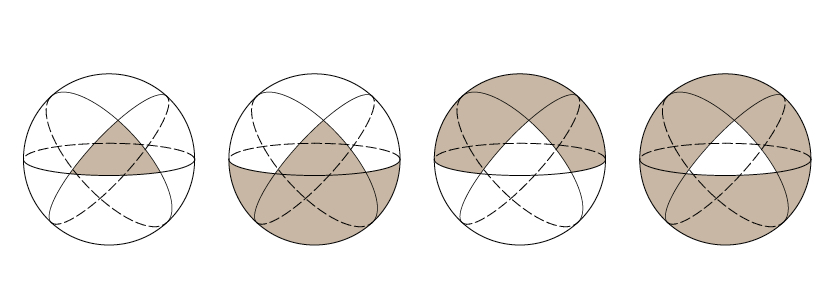
\includegraphics[width=0.9\textwidth]{kugel/Dreieckarten.jpg}
    \captionof{figure}{Dreieckarten auf einer Kugeloberfläche}
\end{center}

Der Begriff Sphärisches Dreieck oder Kugeldreieck ist ein sehr weitläufiger Begriff. 
Dabei können wir den Begriff in drei für uns wesentliche Dreiecke unterteilen:

\begin{itemize}
\item Kugelzweieck
\item Nicht Eulersche’Dreiecke
\item Eulersche’Dreiecke
\end{itemize}

\subsection{Kugelzweieck}

Zwei Grosskreise auf der Kugeloberfläche, zerlegen diese in vier gleiche Kugelzweiecke. 
Jedes dieser Dreieckseiten hat die Länge
$180^{\circ}$ oder $\pi$
Der Flächeninhalt wird dabei nur durch den Winkel $\alpha$ zwischen den beiden Grosskreisen bestimmt.

\begin{center}
        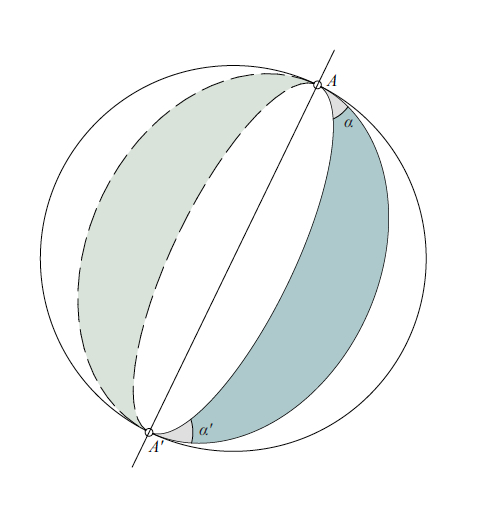
\includegraphics[width=0.3\textwidth]{kugel/Zweieck.jpg}
    \captionof{figure}{Bildung von Zweiecken durch Grosskreise}
\end{center}

Dabei ist der Flächeninhalt der ganzen Kugel:

\begin{align*}
A_{ Kugel } &= 4 \pi r^{2}
\end{align*}


Um den Flächeninhalt des betrachteten Zweieckes zu bekommen, 
müssen wir das ganze noch mit dem Kugelsegment mit dem Winkel $\alpha$ multiplizieren.

\begin{align*}
A_{ Zweieck } &= 4 \pi r^{2} \cdot \frac{ \alpha }{ 2 \pi }
\end{align*}


\subsection{Nicht Eulersche’ Dreiecke}

BLABLA

\subsection{Eulersche’ Dreiecke}

Legt man drei Grosskreise auf eine Kugeloberfläche, bilden sich dabei acht Dreiecke. 
Ein solches Dreieck heisst Eulersches’Dreieck\footnote{%
Leonard Euler (1707-1783), berühmter Schweizer Mathematiker und Physiker. 
Nicht Eulersche’Dreiecke erhält man, indem man das Äussere des Dreieckes ABC betrachtet.} 
Diese Dreiecke werden weder durch die Verlängerung ihrer Seiten durchschnitten, 
noch haben sie Dreiecksseiten welche grösser als $180^{\circ}$ sind.

\begin{center}
        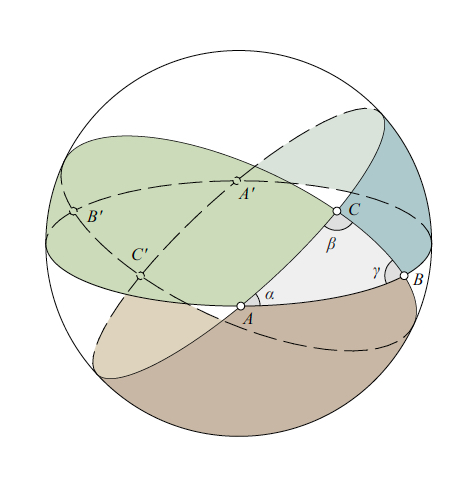
\includegraphics[width=0.4\textwidth]{kugel/Zweiecke.jpg}
    \captionof{figure}{Drei Grosskreise bilden ein sphärisches Dreieck}
\end{center}

In den nachstehenden Erklärungen und Herleitungen, sprechen wir ausschliesslich von Eulerschen’Dreiecken, da die umgeformten Winkelsätze der ebenen Trigonometrie nur auf diese Art von Kugeldreiecken angewendet werden kann.

$A_{ \overline{ ABC }}$ ist die Fläche des Dreieckes auf der Kugeloberfläche
In der ebenen Trigonometrie liegt die Winkelsumme eines Dreiecks bei
$180^{\circ}$.

Anders aber in der sphärischen Trigonometrie. Obschon sie einige Gemeinsamkeiten zur ebenen Trigonometrie aufweist, kann man nicht alles übernehmen.
So auch nicht wie Winkelsumme in einem sphärischen Dreieck.
Diese liegt bei:

\[
\begin{aligned}
\pi
&-
3\pi
&
&\text{\bigg \vert}
&
180^{\circ}
&-
540^{\circ}
\end{aligned}
\]

daraus lässt sich ableiten, das ein einzelner Winkel nicht grösser als $\pi$ oder $180^{\circ}$ sein darf. Ansonsten ist es kein Eulersches’Dreieck und wir dürfen die sphärische Trigonometrie nicht anwenden.\\
Wichtig anzumerken ist, dass die Seiten immer in Radiant beschrieben werden und nicht im Längenmass Meter wie wir es uns gewohnt sind. 
Bei den Dreiecksseiten handelt es sich um Kreisbögen und keine Strecken.

\section{Dreiecksfläche}

\begin{align*}
\text{Zweieck A}
&=
\overline{ABC} + \overline{A'BC} = 2 \alpha r^{ 2 } = A_{ \alpha }\\
\text{Zweieck B}
&=
\overline{ABC} + \overline{AB'C} = 2 \beta r^{ 2 } = A_{ \beta }\\
\text{Zweieck C}
&=
\overline{ABC} + \overline{ABC'} = 2 \gamma r^{ 2 } = A_{ \gamma }
\end{align*}

\begin{align*}
A_{ \alpha } + A_{ \beta } + A_{ \gamma } &= \frac{ 4\pi r^{ 2 } }{ 2 } + 2A_{ \overline{ ABC }} \\
2\alpha r^{ 2 } + 2\beta r^{ 2 } + 2\gamma r^{ 2 } &= \frac{ 4\pi r^{ 2 } }{ 2 } + 2A_{ \overline{ ABC }} \parallel:2\\
\alpha r^{ 2 } + \beta r^{ 2 } + \gamma r^{ 2 } &= \pi r^{ 2 } + A_{ \overline{ ABC }} \parallel-\pi r^{ 2 }\\
r^{ 2 }\left(\alpha + \beta + \gamma - \pi\right) &= A_{ \overline{ ABC }}
\end{align*}




\section{Sphärischer Exzess}
Die Winkelsumme sphärischer Dreiecke ist immer \textgreater \,  $\pi$.

\begin{align*}
\pi < \alpha + \beta + \gamma
\end{align*}

Der sphärische Exzess gibt dabei an, wie stark die Winkelsumme von $\pi$ abweicht.

\begin{align*}
\pi + \epsilon &= \alpha + \beta + \gamma \\
\epsilon &= \alpha + \beta + \gamma - \pi
\end{align*}

Würde der sphärische Exzess in der ebenen Trigonometrie angewendet, wäre dieser = 0. 
Bezieht man das auf die Erde und somit einer Kugel, kann man mit Hilfe eines beliebigen sphärischen Dreieckes und dessen Flächeninhalt auf den Radius der Kugel schliessen.

\subsection{Grenzfall - Satz von Legendre}

\begin{quote} \textit{Ein kleines sphärisches Dreieck kann näherungsweise 
wie ein ebenes Dreieck mit denselben Seiten berechnet 
werden, wenn alle Winkel des ebenen Dreiecks die um 
je ein Drittel des sphärischen Exzesses verminderten 
Winkel des sphärischen Dreiecks nimmt.} \end{quote}
\begin{flushright} - Adrien-Marie Legendre (1752-1833), Paris 1787
\end{flushright}x

Diese Aussage zeigt den Zusammenhang zwischen der 
Trigonometrie in der Ebene sowie in auf der Kugel
auf. Im speziellen bei sehr kleinen sphärischen 
Dreiecken ist die Winkelsumme nur unwesentlich 
grösser als $180^{\circ}$. Des Weiteren kann gesagt werden,
dass der sphärische Exzess gleichmässig auf alle
Winkel aufgeteilt wird.
Wichtig anzumerken ist, dass der Satz von Legendre 
für grosse, aber endliche Radien $r$ gilt.

%[SKIZZE GROSSER RADIUS/KLEINE KRÜMMUNG, KLEINER RADIUS/GROSSE KRÜMMUNG!!!!]
%


\section{Sphärisch Analoge Winkelfunktionen}

\subsection{Sphärischer Sinussatz}

Wir stellen die allgemeinen Sinussätze der Winkel $\alpha$ und $\gamma$ auf:


\[
\begin{aligned}
&{sin(\gamma)} = \frac{h}{a}
&
&\text{\bigg \vert}
&
&{sin(\alpha)} = \frac{h}{c}
&
\end{aligned}
\]

Daraus folgt:
\begin{align*}
h &= sin(\gamma)\cdot a \\
h &= sin(\alpha)\cdot c
\end{align*} 

Durch Gleichsetzung erhält man:
\begin{align*}
h &= h \\
sin(\gamma)\cdot a &= sin(\alpha)\cdot c
\end{align*} 

Durch umstellen erhalten wir den Sinussatz für a und c:
\begin{align*}
sin(\gamma)\cdot a &= sin(\alpha)\cdot c \\
\frac{sin(\gamma)}{c} &= \frac{sin(\alpha)}{a} 
\end{align*} 



\begin{align*}
\frac{sin(\alpha)}{sin(a)} = \frac{sin(\beta)}{sin(b)} = \frac{sin(\gamma)}{sin(c)}
\end{align*} 


\subsection{Winkelkosinussatz}

%[SKIZZE WINKELKOSINUS]

\[
\begin{aligned}
&\overline{C'A'} &= d\cdot {tan(b)}
&
&
&
&
&
&\overline{C'B'} &= d\cdot {tan(a)}
\end{aligned}
\]

\[
\begin{aligned}
&\overline{MA'} &= \frac{ d }{cos(b)}
&
&
&
&
&
&\overline{MB'} &= \frac{ d }{cos(a)}
\end{aligned}
\]

Der allgemeine Kosinussatz beschreibt sich wie folgt:

\begin{align*}
c^{ 2 } &= a^{ 2 } + b^{ 2 } - 2ab \cdot cos(\gamma)
\end{align*}

\begin{align*}
\triangle \overline{A'B'C' }
\overline{ A'B' }^{ 2 } &= \overline{ C'B' }^{ 2 } + \overline{ C'A' }^{ 2 } - 2 \cdot \overline{ C'B' } \cdot \overline{ C'A' } \cdot cos(\gamma)
\end{align*}



\begin{align*}
\overline{A'B'}^{ 2 } &= (d\cdot tan(a))^{ 2 } + (d\cdot tan(b))^{ 2 } - 2 \cdot (d\cdot tan(a) \cdot (d\cdot tan(b) \cdot cos(\gamma)\\
\overline{A'B'}^{ 2 } &= d^{ 2 } \cdot \left(\left(tan^{ 2 }(a) + tan^{ 2 }(b)\right) - 2\cdot tan(a) \cdot tan(b) \cdot cos(\gamma)\right)
\end{align*}

\begin{align*}
\triangle \overline{ MA'B' }
\overline{ A'B' }^{ 2 } &= \overline{ MB' }^{ 2 } + \overline{ MA' }^{ 2 } - 2\cdot \overline{ MB'} \cdot \overline{ MA' } \cdot cos(c)
\end{align*}


\begin{align*}
\overline{ A'B'}^{ 2 } &= \left(\frac{ d }{ cos(a) }  \right)^{ 2 } + \left(\frac{ d }{ cos(b)}  \right)^{ 2 } - 2 \cdot \frac{ d }{ cos(a)} \cdot \frac{ d }{ cos(b)} \cdot cos(c) \\
\overline{ A'B' }^{ 2 } &= d^{ 2 } \cdot \left(\left(\frac{ 1 }{ cos(a) }  \right)^{ 2 } + \left(\frac{ 1 }{ cos(b) }  \right)^{ 2 } - 2 \cdot \frac{ 1 }{ cos(a)} \cdot \frac{ 1 }{ cos(b)} \cdot cos(c)\right)\\
\overline{ A'B' }^{ 2 } &= d^{ 2 } \cdot \left(\left(tan^{ 2 }(a) + 1\right) + \left(tan^{ 2 }(b) + 1\right) - \left(2 \cdot \frac{cos(c)}{cos(a) \cdot cos(b)}\right)\right)
\end{align*}



\begin{align*}
\overline{ A'B'}^{ 2 } &= d^{ 2 } \cdot \left(\left(tan^{ 2 }(a) + tan^{ 2 }(b)\right) - 2 \cdot tan(a) \cdot tan(b) \cdot cos(\gamma)\right) \\
\overline{ A'B'}^{ 2 } &= d^{ 2 } \cdot \left(\left(tan^{ 2 }(a) + 1\right) + \left(tan^{ 2 }(b) + 1\right) - \left(2 \cdot \frac{cos(c)}{cos(a) \cdot cos(b)}\right)\right)
\end{align*}

Die anderen Gleichungen des Satzes, erfolgen aus Symmetriegründen.

\subsection{Seitenkosinussatz}
Durch zyklische Vertauschung des Winkelkosinus erhalten wir den Seitenkosinussatz:

\begin{align*}
{cos(a)} &= {cos(b)} \cdot {cos(c)} + {sin(b)} \cdot {sin(c)} \cdot {sin(\alpha)}\\
{cos(b)} &= {cos(a)} \cdot {cos(c)} + {sin(a)} \cdot {sin(c)} \cdot {sin(\beta)}\\
{cos(c)} &= {cos(a)} \cdot {cos(b)} + {sin(a)} \cdot {sin(b)} \cdot {sin(\gamma)}\\
\end{align*}

\section{Navigation auf See}
Das besondere an Seekarten ist die Inhaltliche Ausrichtung. Anders wie Landkarten muss sie Informationen enthalten welche für den Kapitän und seine Besatzung von grosser Bedeutung sind. Vor allem in Küstennähe ist das navigieren eines Schiffes besonders gefährlich. So enthalten Seekarten etwas über Wassertiefen, Bodenbeschaffenheiten, Gezeiten, Küstenlinien, Landzungen und Windrichtungen.
Der Hauptunterschied dabei ist, das auf der Landkarte feste Positionen definiert und aufgezeigt werden, das einzige was sich verändert ist der Reisende selbst. Bei der Seekarte ist das anders, es werden veränderliche Einwirkungen der Natur festgehalten.

Dieser kleine Unterschied zeigt die Notwendigkeit auf, die Position und den Kurs seines Schiffes auf See immer ermitteln zu können.


\section{Geographische Koordinaten}

Nachdem klar war, das die Erde eine Kugel ist, wurde diese in ein Gradnetz aufgeteilt. Dabei wurden die Angaben für eine exakte Ortsbestimmung klar definiert und die bis heute gültigen Koordinaten bestimmt.
Dabei muss man sich nochmals in Erinnerung rufen, dass sich die Erde in 24h einmal um ihre eigene Achse dreht. Nach $360 ^{\circ}$ 
und somit einer vollen Umdrehung, steht sie wieder in ihrer Ursprungsposition und ein neuer Tag beginnt.

Die Koordinaten setzen sich aus folgenden Komponenten zusammen:

\[
\begin{aligned}
&\text{Grad } (^{\circ})
&
&\text{\bigg \vert}
&
&\text{Bogenminuten } (`)
&
&\text{\bigg \vert}
&
&\text{Bogensekunden } (``)
\end{aligned}
\]

Die Erdoberfläche wurde in je 360 Breiten- und Längengrade eingeteilt. Die Breitengrade haben zueinander einen Abstand von 111.31 km, dies entspricht auch dem Abstand der Längengrade am Äquator mit Zunehmender Nähe zu den Polen, nimmt dieser Abstand ab.

\[
\begin{aligned}
&1^{\circ}
&
&\text{\bigg \vert}
&
&4 \text{ Minuten}
&
&\text{\bigg \vert}
&
&111.31\text{ km}
\end{aligned}
\]

Berechnet man nun die Erdumdrehung von 360°, erhält man genau den Erdumfang am Äquator: \begin{align*} 40’074 \text{ km.}\end{align*}

Dabei geben die Bogenminuten und -sekunden dem Standort die gewünschte Exaktheit. Mit den vollständigen Koordinaten lässt sich der Standort auf einer Landkarte exakt bestimmen und einzeichnen.

\subsection{Zeitzonen der Erde}
Wenn man nun die verschiedenen Zeitzonen der Erde betrachtet, macht die Verschiebung von jeweils einer Stunde durchaus Sinn, es lässt sich auf die Längengrade schliessen.
Zwischen den verschiedenen Zeitzonen liegen 15 Längengrade:

\begin{align*}
\text{15 Längengrade à 4 Minuten = 60 Minuten Zeitverschiebung = ca. 1665 km}
\end{align*}

Dabei ist die Zeitzone in welcher Mitte sich der Greenwich Meredian befindet die \textit{Greenwich Mean Time (GMT)} welche bis 1928 als Weltzeit galt. Im Jahr 1972 wurde diese umbenannt in die \textit{Coordinated Universal Time (UTC)} und wir von da an als Weltzeit $\pm$ 0.00 verwendet.


\section{Der Breitengrad}
Die Breitengrade bilden die bereits genannten Kleinkreise auf der Kugeloberfläche. Sie verlaufen in einem Abstand von genau 111 km parallel zum Äquator. Dabei stellt  dieser genau die Mitte zwischen Nord- und Südpol dar und teilt die Erdkugel in zwei gleiche Hälften. Somit wird von nördlicher und südlicher Breite gesprochen, je nach dem auf welcher Halbkugel man sich befindet.

%[SKIZZE DER GEOGRAFISCHEN BREITE ERDKUGEL]

\subsection{Geografische Breite $\phi$}
\begin{definition}
Die geografische Breite eines Standortes ist nichts anderes, als der Winkel am Erdmittelpunkt zwischen der Ebene des Äquators und der Geraden zum Standpunkt auf der Erdoberfläche.
\end{definition}

%[SKIZZE DER GEOGRAFISCHEN BREITE MIT WINKEL]

\subsection{Navigation mit den Breitengraden}
Da der Breitengrad bereits sehr früh ziemlich präzise bestimmt werden könnte, nutzten bereits die Seefahrer um Christoph Kolumbus den Breitengrad zur Navigation ihrer Flotten.
Den dieser lässt sich ziemlich einfach aus dem höchsten Sonnenstand oder einem Fixstern bestimmen. Dabei wird mit einem Jakobsstab\footnote{%
Der Jakobsstab ist ein früheres astronomisches Instrument zur Winkelmessung und wurde vor allem in der Seefahrt verwendet. Er ist in der Nautik der Vorläufer des Sextanten.} (später Sextant\footnote{%
Der Sextant ist ein nautisches Messinstrument zur Winkelmessung von Horizont und Fixstern (Gestirn)}) der Winkel zwischen dem Horizont und dem Fixstern gemessen. Der Winkel welchen man erhält, zieht man von 90° ab und erhält somit die geografische Breite. \\

%[SKIZZE ERMITTLUNG DES BREITENGRADES]

Wenn man sich auf der Nordhalbkugel befindet, ist der Polarstern ein sehr guter Fixstern. Befindet sich ein Schiff nun sehr nahe am Nordpol, steht dieser nahezu senkrecht am Himmelszelt bei $90^{\circ}$. Würde es aber nahe dem Äquator stehen, erscheint dieser am Horizont bei $0^{\circ}$.

\subsection{Korrekturbeiwert}

\section{Der Längengrad}
Die Längengrade bilden die bereits genannten Grosskreise auf der Kugeloberfläche.
Sie schneiden den Äquator im rechten Winkel, haben dort einen Abstand von 111 km zueinander und verbinden die Pole. Anders wie bei der geografischen Breite, ist in der Natur kein Längengrad gegeben welcher den Nullpunkt darstellt.

%[SKIZZE DER GEOGRAFISCHEN LÄNGE ERDKUGEL]

\subsection{Geografische Länge $\lambda$}
\begin{definition}
Die geografische Länge ist der Winkel an der Erdachse zum Nullmeridian.
\end{definition}

\subsection{Navigation mit den Längengraden}
Die geografische Länge lässt sich nicht so einfach bestimmen wie deren Breite. Für die Berechnung auf See benötigt man eine Referenzzeit eines Ortes mit bekannter Länge.
In der Zeit der Entdecker gab es noch keine mechanischen Uhren. Die Sonnenuhr war zudem ungeeignet, da diese nur die Uhrzeit am Standort mass und nicht die am Referenzort selbst. Die erste Pendeluhr wurde erst Mitte des 17. Jahrhunderts erfunden, was in der Schifffahrt aber auch nicht die Lösung brachte.\\
Pendeluhren auf einem Schiff sind ungeeignet, da das Pendel mit dem Wellengang aus dem Takt gebracht wird und somit die Uhr falsch geht.
Zu ungenau und gegen äussere Erschütterungen zu empfindlich waren später auch die federgetriebenen Uhren und die Unruh. Dazukamen die verschiedenen Klimazonen welche ein Schiff zu durchqueren hatten. Das Metall zog sich viel zu fest zusammen oder dehnte sich aus, was dazu führte das die Uhr unregelmässig lief.

Das sogenannte „Längenproblem“ stellte nicht nur bei der Navigation auf See ein Problem dar, es ergaben sich auch wirtschaftliche Konsequenzen. Die Schiffe mussten bis zur gewünschten geografischen Breite navigieren und segelten dann den Breitengrad entlang. Dabei waren die Schiffe oft Wochenlang unterwegs und segelten die „Breiten ab“ um an die gewünschte Position zu kommen. Dies führte zu erheblichen Zeitverlusten und viel längeren Reisezeiten.


\section{The Board of Longitude - Das Längenproblem}
Das Längenproblem beschäftigte alle grossen Seefahrernationen Europas. Wenn man bedenkt das sich Werte in einer  Höhe von halben britischen Staatshaushalten auf verloren gegangenen Schiffen befanden, erkennt man die Dringlichkeit für eine zuverlässige und genaue Navigation auf See.


\begin{itemize}
\item £ 20’000 - Abweichung von max. einem halben Grad
\item £ 15’000 - Abweichung von zwei Drittel Grad
\item £ 10’000 - Abweichung von max. $1 ^{\circ}$
\end{itemize}

\subsection{John Harrison}


\subsection{Tobias Mayer}



Uhren mit einer Abweichung von einer Minute Abweichung pro Tag (





\section{Nautische Dreieck}


$\Rightarrow$





\section{Die Vermessung der Welt}
Wir schreiben das Jahr 1818 und kehren in die Zeit des Mathematikers Carl Friedrich Gauss zurück. Neben dem liebevoll genannten „kleinen Gauss“ und anderen herausragenden Mathematischen Leistungen, beschäftigte er in den Folgejahren mit der Vermessung des Königreichs Hannovers und verfasste auf 61 Blättern das Kartenwerk \textit{Gauss’sche Landesaufnahme der 1815 durch Hannover erworbenen Gebiete}.






AUFGABE

Hubble Teleskop 
24. April 1990






\printbibliography[heading=subbibliography]
\end{refsection}




%\chapter{Geometrie auf der Kugeloberfläche\label{chapter:kugel}}
\lhead{Geometrie auf der Kugeloberfläche}
\begin{refsection}
\chapterauthor{Melina Staub und Fabian Schmid}

\section{Einleitung}

Schon seit jeher fasziniert den Menschen die Fahrt zur See. Nicht grundlos ist die Seefahrt eine der wichtigsten und ältesten Tätigkeiten der Menschheit. Der innerliche Drang neue Weltmeere und unbekannte Gebiete zu entdecken, die Fahrt zur See zu erleichtern und erträglicher zu machen, trieben die Menschen an, die Schiffe dieser Welt immer weiter zu entwickeln.

Die Idee der Kugelform der Erde ist älter als man zu denken vermag. Bereits der Schüler des antiken griechischen Philosophen Platon - Aristoteles schrieb in seiner Schrift \textit{Über den Himmel} aus dem 4. Jahrhundert v. Chr. etliche Gründe welche für die Gestallt der Erde als Kugel sprechen:

\begin{itemize}
      \item Sämtliche schweren Körper streben zum Mittelpunkt des Alls. Da sie dies von allen Seiten her gleichmäßig tun und die Erde im Mittelpunkt des Alls steht, muss sie eine kugelrunde Gestalt annehmen. 
\item Bei von der Küste wegfahrende Schiffen wird der Rumpf vor den Segeln der Sicht verborgen. 
\item In südlichen Ländern erscheinen südliche Sternbilder höher über dem Horizont.
\item Der Erdschatten bei einer Mondfinsternis ist stets rund.
\end{itemize}

Jedoch war um 1492 - der Zeit der Entdeckung Amerikas durch Christoph Kolumbus, die Idee der Erde in Kugelform noch sehr umstritten. Er erkannte anhand den Theorien und Erkenntnissen der alten Griechen, vor allem Aristoteles, das die Erde eine Kugel sein muss. \\
Doch mit seinem Vorschlag einen Seeweg über den Atlantik nach Indien zu finden und nicht wie üblich um Afrika zu segeln, stiess er beim beim portugiesischen König auf taube Ohren. Sein Plan Indien über eine Route nach Westen zu erreichen, widersprach dem gesunden Menschenverstand. Wäre die Erde wirklich eine Kugel und man befände sich auf der unteren Erdhalbkugel, würde man herunterfallen.\\
Doch auch der damals übliche Glaube an die Erde in Scheibenform brachte so einige Risiken mit sich. Was würde passieren, wenn die Flotte das Ende der Scheibe erreicht hatte? Würden sie über den Erdrand hinweggleiten und in den Abgrund stürzen?\\
Erst nach viel Überzeugungsarbeit durch Kolumbus, setzte er sich am Spanischen Hof durch und segelte über die Westliche Route über den Atlantik und entdeckte schlussendlich Amerika.

Der praktische und greifbare Beweis das die Erde eine Kugel ist, lieferte rund 30 Jahre später der Portugiese Fernando Magellan. Mit seiner Weltumsegelung und seiner Ankunft in den Philippinen, bewies er definitiv das die Erde eine Kugel ist.\\

Nun wollen wir uns die Frage stellen, wie die alten Seefahrer ohne GPS und jeglichen modernen Navigationssystemen auf hoher See wussten wo sie sich befinden und was haben die Sterne mit alldem zu tun? Reisen Sie mit uns zurück in eine Zeit mit Sextant, Kompass und Sternkarten. In die Zeit der Seefahrer und Entdecker.


\section{Geometrie auf der Ebene und der Kugel}

Euklid von Alexandria beschrieb die Grundbegriffe der ebenen Geometrie mittels Punkt, Geraden, Ebene, Winkel und Dreieck. Diese Dreiecke lassen sich mithilfe der ebenen Trigonometrie beschreiben. Dabei gelten die uns bekannten trigonometrischen Winkelfunktionen:\\

\text{Sinussatz:}
\begin{align*}
\frac{ a }{ sin(\alpha) } &= \frac{ b }{sin(\beta)} = \frac{ c }{ sin(\gamma) } = \frac{abc}{2A} = 2r\\
\end{align*}

\text{Cosinussatz:}
\begin{align*}
c^{ 2 } &= a^{ 2 } + b^{ 2 } - 2ab\cdot cos(\gamma)\\
b^{ 2 } &= a^{ 2 } + c^{ 2 } - 2ab\cdot cos(\beta)\\
a^{ 2 } &= b^{ 2 } + c^{ 2 } - 2ab\cdot cos(\alpha)
\end{align*}

Um Dreiecke auf der Kugeloberfläche zu berechnen, benötigt man die sphärische Trigonometrie. Die oben beschriebenen Sätze lassen sich auf der Kugel nicht anwenden, sie werden aber als Grundlage zur Herleitung der Sätze für das Kugeldreieck benötigt.

Die nachfolgenden Seiten thematisieren die Geometrie auf der Kugeloberfläche und wie sie in der Navigation eingesetzt werden kann.


\section{Gross- und Kleinkreise}

Eine Kugeloberfläche lässt sich in zwei verschiedene Kreisarten einteilen -  Gross- und Kleinkreise. 
Wir betrachten als erstes die Grosskreise:

\begin{definition}
Ein Großkreis ist ein größtmöglicher Kreis auf einer Kugeloberfläche. Sein Mittelpunkt fällt immer mit dem Mittelpunkt der Kugel zusammen und ein Schnitt auf dem Großkreis teilt die Kugel in jedem Fall in zwei („gleich große“) Hälften.
\end{definition}

Es gibt unendlich viele Möglichkeiten, eine Kugel in zwei gleich grosse Stücke zu zerschneiden, 
daher gibt es auch unendlich viele Grosskreise. Wenn wir die Grosskreise auf einer Kugel mit diesen auf der Erde beschreiben, sprechen wir von den Längengraden aber auch der Äquator beschreibt einen Grosskreis.
Ein Elementarer Bestandteil bilden die Grosskreise in der sphärischen Trigonometrie. Mithilfe der Schnittpunkte verschiedener Grosskreise, lässt sich ein Sphärisches Dreieck bilden auf welchem sich die sphärische Trigonometrie anwenden lässt.

[GRAFIK GROSSKREISE]

\begin{definition}
Unter Kleinkreis versteht man jene Kreise auf einer Kugeloberfläche, deren Ebenen nicht den Kugelmittelpunkt enthalten.
\end{definition}

Die Kleinkreise eignen sich im Gegensatz zu den Grosskreisen \textit{nicht} für die sphärische Trigonometrie. 
Sie werden lediglich zur Bestimmung der Messgrössen, Winkelabstände oder des Höhenwinkels eines Gestirns verwendet. 

Wenn wir die Kleinkreise auf die Erdoberfläche projizieren betrachten wir die Breitengrade.

[GRAFIK KLEINKREISE]


\section{Sphärische Dreiecke / Kugeldreieck}

\begin{center}
        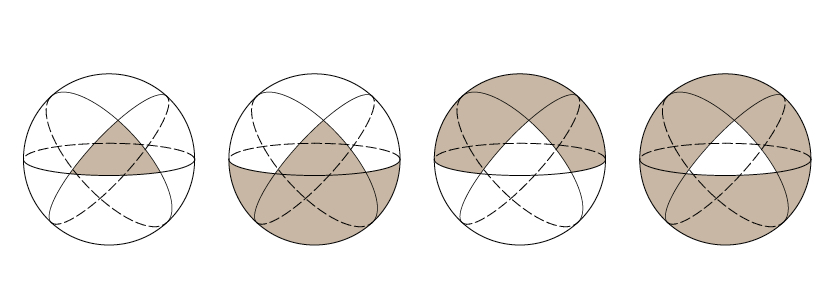
\includegraphics[width=0.9\textwidth]{kugel/Dreieckarten.jpg}
    \captionof{figure}{Dreieckarten auf einer Kugeloberfläche}
\end{center}

Der Begriff Sphärisches Dreieck oder Kugeldreieck ist ein sehr weitläufiger Begriff. 
Dabei können wir den Begriff in drei für uns wesentliche Dreiecke unterteilen:

\begin{itemize}
\item Kugelzweieck
\item Nicht Eulersche’Dreiecke
\item Eulersche’Dreiecke
\end{itemize}

\subsection{Kugelzweieck}

Zwei Grosskreise auf der Kugeloberfläche, zerlegen diese in vier gleiche Kugelzweiecke. 
Jedes dieser Dreieckseiten hat die Länge
$180^{\circ}$ oder $\pi$
Der Flächeninhalt wird dabei nur durch den Winkel $\alpha$ zwischen den beiden Grosskreisen bestimmt.

\begin{center}
        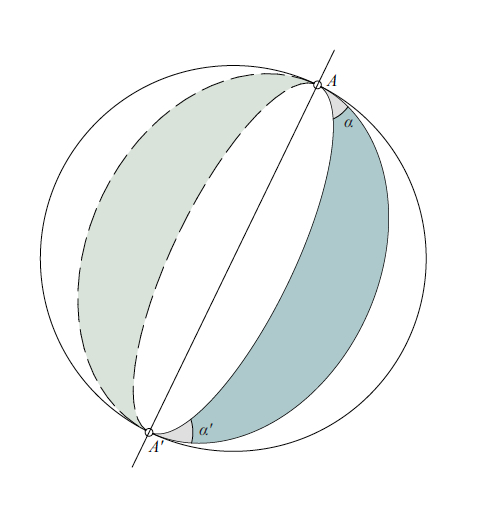
\includegraphics[width=0.3\textwidth]{kugel/Zweieck.jpg}
    \captionof{figure}{Bildung von Zweiecken durch Grosskreise}
\end{center}

Dabei ist der Flächeninhalt der ganzen Kugel:

\begin{align*}
A_{ Kugel } &= 4 \pi r^{2}
\end{align*}


Um den Flächeninhalt des betrachteten Zweieckes zu bekommen, 
müssen wir das ganze noch mit dem Kugelsegment mit dem Winkel $\alpha$ multiplizieren.

\begin{align*}
A_{ Zweieck } &= 4 \pi r^{2} \cdot \frac{ \alpha }{ 2 \pi }
\end{align*}


\subsection{Nicht Eulersche’ Dreiecke}

BLABLA

\subsection{Eulersche’ Dreiecke}

Legt man drei Grosskreise auf eine Kugeloberfläche, bilden sich dabei acht Dreiecke. 
Ein solches Dreieck heisst Eulersches’Dreieck\footnote{%
Leonard Euler (1707-1783), berühmter Schweizer Mathematiker und Physiker. 
Nicht Eulersche’Dreiecke erhält man, indem man das Äussere des Dreieckes ABC betrachtet.} 
Diese Dreiecke werden weder durch die Verlängerung ihrer Seiten durchschnitten, 
noch haben sie Dreiecksseiten welche grösser als $180^{\circ}$ sind.

\begin{center}
        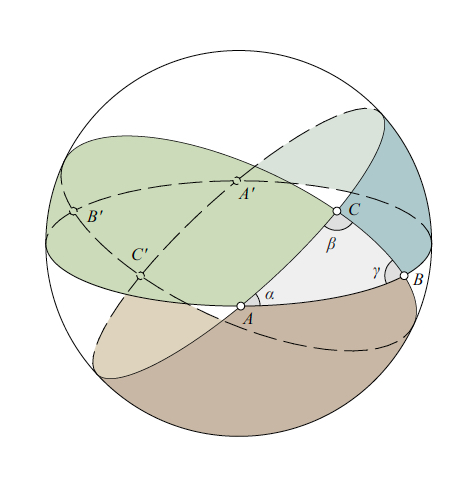
\includegraphics[width=0.4\textwidth]{kugel/Zweiecke.jpg}
    \captionof{figure}{Drei Grosskreise bilden ein sphärisches Dreieck}
\end{center}

In den nachstehenden Erklärungen und Herleitungen, sprechen wir ausschliesslich von Eulerschen’Dreiecken, da die umgeformten Winkelsätze der ebenen Trigonometrie nur auf diese Art von Kugeldreiecken angewendet werden kann.

$A_{ \overline{ ABC }}$ ist die Fläche des Dreieckes auf der Kugeloberfläche
In der ebenen Trigonometrie liegt die Winkelsumme eines Dreiecks bei
$180^{\circ}$.

Anders aber in der sphärischen Trigonometrie. Obschon sie einige Gemeinsamkeiten zur ebenen Trigonometrie aufweist, kann man nicht alles übernehmen.
So auch nicht wie Winkelsumme in einem sphärischen Dreieck.
Diese liegt bei:

\[
\begin{aligned}
\pi
&-
3\pi
&
&\text{\bigg \vert}
&
180^{\circ}
&-
540^{\circ}
\end{aligned}
\]

daraus lässt sich ableiten, das ein einzelner Winkel nicht grösser als $\pi$ oder $180^{\circ}$ sein darf. Ansonsten ist es kein Eulersches’Dreieck und wir dürfen die sphärische Trigonometrie nicht anwenden.\\
Wichtig anzumerken ist, dass die Seiten immer in Radiant beschrieben werden und nicht im Längenmass Meter wie wir es uns gewohnt sind. 
Bei den Dreiecksseiten handelt es sich um Kreisbögen und keine Strecken.

\section{Dreiecksfläche}

\begin{align*}
\text{Zweieck A}
&=
\overline{ABC} + \overline{A'BC} = 2 \alpha r^{ 2 } = A_{ \alpha }\\
\text{Zweieck B}
&=
\overline{ABC} + \overline{AB'C} = 2 \beta r^{ 2 } = A_{ \beta }\\
\text{Zweieck C}
&=
\overline{ABC} + \overline{ABC'} = 2 \gamma r^{ 2 } = A_{ \gamma }
\end{align*}

\begin{align*}
A_{ \alpha } + A_{ \beta } + A_{ \gamma } &= \frac{ 4\pi r^{ 2 } }{ 2 } + 2A_{ \overline{ ABC }} \\
2\alpha r^{ 2 } + 2\beta r^{ 2 } + 2\gamma r^{ 2 } &= \frac{ 4\pi r^{ 2 } }{ 2 } + 2A_{ \overline{ ABC }} \parallel:2\\
\alpha r^{ 2 } + \beta r^{ 2 } + \gamma r^{ 2 } &= \pi r^{ 2 } + A_{ \overline{ ABC }} \parallel-\pi r^{ 2 }\\
r^{ 2 }\left(\alpha + \beta + \gamma - \pi\right) &= A_{ \overline{ ABC }}
\end{align*}




\section{Sphärischer Exzess}
Die Winkelsumme sphärischer Dreiecke ist immer \textgreater \,  $\pi$.

\begin{align*}
\pi < \alpha + \beta + \gamma
\end{align*}

Der sphärische Exzess gibt dabei an, wie stark die Winkelsumme von $\pi$ abweicht.

\begin{align*}
\pi + \epsilon &= \alpha + \beta + \gamma \\
\epsilon &= \alpha + \beta + \gamma - \pi
\end{align*}

Würde der sphärische Exzess in der ebenen Trigonometrie angewendet, wäre dieser = 0. 
Bezieht man das auf die Erde und somit einer Kugel, kann man mit Hilfe eines beliebigen sphärischen Dreieckes und dessen Flächeninhalt auf den Radius der Kugel schliessen.

\subsection{Grenzfall - Satz von Legendre}

\begin{quote} \textit{Ein kleines sphärisches Dreieck kann näherungsweise 
wie ein ebenes Dreieck mit denselben Seiten berechnet 
werden, wenn alle Winkel des ebenen Dreiecks die um 
je ein Drittel des sphärischen Exzesses verminderten 
Winkel des sphärischen Dreiecks nimmt.} \end{quote}
\begin{flushright} - Adrien-Marie Legendre (1752-1833), Paris 1787
\end{flushright}x

Diese Aussage zeigt den Zusammenhang zwischen der 
Trigonometrie in der Ebene sowie in auf der Kugel
auf. Im speziellen bei sehr kleinen sphärischen 
Dreiecken ist die Winkelsumme nur unwesentlich 
grösser als $180^{\circ}$. Des Weiteren kann gesagt werden,
dass der sphärische Exzess gleichmässig auf alle
Winkel aufgeteilt wird.
Wichtig anzumerken ist, dass der Satz von Legendre 
für grosse, aber endliche Radien $r$ gilt.

%[SKIZZE GROSSER RADIUS/KLEINE KRÜMMUNG, KLEINER RADIUS/GROSSE KRÜMMUNG!!!!]
%


\section{Sphärisch Analoge Winkelfunktionen}

\subsection{Sphärischer Sinussatz}

Wir stellen die allgemeinen Sinussätze der Winkel $\alpha$ und $\gamma$ auf:


\[
\begin{aligned}
&{sin(\gamma)} = \frac{h}{a}
&
&\text{\bigg \vert}
&
&{sin(\alpha)} = \frac{h}{c}
&
\end{aligned}
\]

Daraus folgt:
\begin{align*}
h &= sin(\gamma)\cdot a \\
h &= sin(\alpha)\cdot c
\end{align*} 

Durch Gleichsetzung erhält man:
\begin{align*}
h &= h \\
sin(\gamma)\cdot a &= sin(\alpha)\cdot c
\end{align*} 

Durch umstellen erhalten wir den Sinussatz für a und c:
\begin{align*}
sin(\gamma)\cdot a &= sin(\alpha)\cdot c \\
\frac{sin(\gamma)}{c} &= \frac{sin(\alpha)}{a} 
\end{align*} 



\begin{align*}
\frac{sin(\alpha)}{sin(a)} = \frac{sin(\beta)}{sin(b)} = \frac{sin(\gamma)}{sin(c)}
\end{align*} 


\subsection{Winkelkosinussatz}

%[SKIZZE WINKELKOSINUS]

\[
\begin{aligned}
&\overline{C'A'} &= d\cdot {tan(b)}
&
&
&
&
&
&\overline{C'B'} &= d\cdot {tan(a)}
\end{aligned}
\]

\[
\begin{aligned}
&\overline{MA'} &= \frac{ d }{cos(b)}
&
&
&
&
&
&\overline{MB'} &= \frac{ d }{cos(a)}
\end{aligned}
\]

Der allgemeine Kosinussatz beschreibt sich wie folgt:

\begin{align*}
c^{ 2 } &= a^{ 2 } + b^{ 2 } - 2ab \cdot cos(\gamma)
\end{align*}

\begin{align*}
\triangle \overline{A'B'C' }
\overline{ A'B' }^{ 2 } &= \overline{ C'B' }^{ 2 } + \overline{ C'A' }^{ 2 } - 2 \cdot \overline{ C'B' } \cdot \overline{ C'A' } \cdot cos(\gamma)
\end{align*}



\begin{align*}
\overline{A'B'}^{ 2 } &= (d\cdot tan(a))^{ 2 } + (d\cdot tan(b))^{ 2 } - 2 \cdot (d\cdot tan(a) \cdot (d\cdot tan(b) \cdot cos(\gamma)\\
\overline{A'B'}^{ 2 } &= d^{ 2 } \cdot \left(\left(tan^{ 2 }(a) + tan^{ 2 }(b)\right) - 2\cdot tan(a) \cdot tan(b) \cdot cos(\gamma)\right)
\end{align*}

\begin{align*}
\triangle \overline{ MA'B' }
\overline{ A'B' }^{ 2 } &= \overline{ MB' }^{ 2 } + \overline{ MA' }^{ 2 } - 2\cdot \overline{ MB'} \cdot \overline{ MA' } \cdot cos(c)
\end{align*}


\begin{align*}
\overline{ A'B'}^{ 2 } &= \left(\frac{ d }{ cos(a) }  \right)^{ 2 } + \left(\frac{ d }{ cos(b)}  \right)^{ 2 } - 2 \cdot \frac{ d }{ cos(a)} \cdot \frac{ d }{ cos(b)} \cdot cos(c) \\
\overline{ A'B' }^{ 2 } &= d^{ 2 } \cdot \left(\left(\frac{ 1 }{ cos(a) }  \right)^{ 2 } + \left(\frac{ 1 }{ cos(b) }  \right)^{ 2 } - 2 \cdot \frac{ 1 }{ cos(a)} \cdot \frac{ 1 }{ cos(b)} \cdot cos(c)\right)\\
\overline{ A'B' }^{ 2 } &= d^{ 2 } \cdot \left(\left(tan^{ 2 }(a) + 1\right) + \left(tan^{ 2 }(b) + 1\right) - \left(2 \cdot \frac{cos(c)}{cos(a) \cdot cos(b)}\right)\right)
\end{align*}



\begin{align*}
\overline{ A'B'}^{ 2 } &= d^{ 2 } \cdot \left(\left(tan^{ 2 }(a) + tan^{ 2 }(b)\right) - 2 \cdot tan(a) \cdot tan(b) \cdot cos(\gamma)\right) \\
\overline{ A'B'}^{ 2 } &= d^{ 2 } \cdot \left(\left(tan^{ 2 }(a) + 1\right) + \left(tan^{ 2 }(b) + 1\right) - \left(2 \cdot \frac{cos(c)}{cos(a) \cdot cos(b)}\right)\right)
\end{align*}

Die anderen Gleichungen des Satzes, erfolgen aus Symmetriegründen.

\subsection{Seitenkosinussatz}
Durch zyklische Vertauschung des Winkelkosinus erhalten wir den Seitenkosinussatz:

\begin{align*}
{cos(a)} &= {cos(b)} \cdot {cos(c)} + {sin(b)} \cdot {sin(c)} \cdot {sin(\alpha)}\\
{cos(b)} &= {cos(a)} \cdot {cos(c)} + {sin(a)} \cdot {sin(c)} \cdot {sin(\beta)}\\
{cos(c)} &= {cos(a)} \cdot {cos(b)} + {sin(a)} \cdot {sin(b)} \cdot {sin(\gamma)}\\
\end{align*}

\section{Navigation auf See}
Das besondere an Seekarten ist die Inhaltliche Ausrichtung. Anders wie Landkarten muss sie Informationen enthalten welche für den Kapitän und seine Besatzung von grosser Bedeutung sind. Vor allem in Küstennähe ist das navigieren eines Schiffes besonders gefährlich. So enthalten Seekarten etwas über Wassertiefen, Bodenbeschaffenheiten, Gezeiten, Küstenlinien, Landzungen und Windrichtungen.
Der Hauptunterschied dabei ist, das auf der Landkarte feste Positionen definiert und aufgezeigt werden, das einzige was sich verändert ist der Reisende selbst. Bei der Seekarte ist das anders, es werden veränderliche Einwirkungen der Natur festgehalten.

Dieser kleine Unterschied zeigt die Notwendigkeit auf, die Position und den Kurs seines Schiffes auf See immer ermitteln zu können.


\section{Geographische Koordinaten}

Nachdem klar war, das die Erde eine Kugel ist, wurde diese in ein Gradnetz aufgeteilt. Dabei wurden die Angaben für eine exakte Ortsbestimmung klar definiert und die bis heute gültigen Koordinaten bestimmt.
Dabei muss man sich nochmals in Erinnerung rufen, dass sich die Erde in 24h einmal um ihre eigene Achse dreht. Nach $360 ^{\circ}$ 
und somit einer vollen Umdrehung, steht sie wieder in ihrer Ursprungsposition und ein neuer Tag beginnt.

Die Koordinaten setzen sich aus folgenden Komponenten zusammen:

\[
\begin{aligned}
&\text{Grad } (^{\circ})
&
&\text{\bigg \vert}
&
&\text{Bogenminuten } (`)
&
&\text{\bigg \vert}
&
&\text{Bogensekunden } (``)
\end{aligned}
\]

Die Erdoberfläche wurde in je 360 Breiten- und Längengrade eingeteilt. Die Breitengrade haben zueinander einen Abstand von 111.31 km, dies entspricht auch dem Abstand der Längengrade am Äquator mit Zunehmender Nähe zu den Polen, nimmt dieser Abstand ab.

\[
\begin{aligned}
&1^{\circ}
&
&\text{\bigg \vert}
&
&4 \text{ Minuten}
&
&\text{\bigg \vert}
&
&111.31\text{ km}
\end{aligned}
\]

Berechnet man nun die Erdumdrehung von 360°, erhält man genau den Erdumfang am Äquator: \begin{align*} 40’074 \text{ km.}\end{align*}

Dabei geben die Bogenminuten und -sekunden dem Standort die gewünschte Exaktheit. Mit den vollständigen Koordinaten lässt sich der Standort auf einer Landkarte exakt bestimmen und einzeichnen.

\subsection{Zeitzonen der Erde}
Wenn man nun die verschiedenen Zeitzonen der Erde betrachtet, macht die Verschiebung von jeweils einer Stunde durchaus Sinn, es lässt sich auf die Längengrade schliessen.
Zwischen den verschiedenen Zeitzonen liegen 15 Längengrade:

\begin{align*}
\text{15 Längengrade à 4 Minuten = 60 Minuten Zeitverschiebung = ca. 1665 km}
\end{align*}

Dabei ist die Zeitzone in welcher Mitte sich der Greenwich Meredian befindet die \textit{Greenwich Mean Time (GMT)} welche bis 1928 als Weltzeit galt. Im Jahr 1972 wurde diese umbenannt in die \textit{Coordinated Universal Time (UTC)} und wir von da an als Weltzeit $\pm$ 0.00 verwendet.


\section{Der Breitengrad}
Die Breitengrade bilden die bereits genannten Kleinkreise auf der Kugeloberfläche. Sie verlaufen in einem Abstand von genau 111 km parallel zum Äquator. Dabei stellt  dieser genau die Mitte zwischen Nord- und Südpol dar und teilt die Erdkugel in zwei gleiche Hälften. Somit wird von nördlicher und südlicher Breite gesprochen, je nach dem auf welcher Halbkugel man sich befindet.

%[SKIZZE DER GEOGRAFISCHEN BREITE ERDKUGEL]

\subsection{Geografische Breite $\phi$}
\begin{definition}
Die geografische Breite eines Standortes ist nichts anderes, als der Winkel am Erdmittelpunkt zwischen der Ebene des Äquators und der Geraden zum Standpunkt auf der Erdoberfläche.
\end{definition}

%[SKIZZE DER GEOGRAFISCHEN BREITE MIT WINKEL]

\subsection{Navigation mit den Breitengraden}
Da der Breitengrad bereits sehr früh ziemlich präzise bestimmt werden könnte, nutzten bereits die Seefahrer um Christoph Kolumbus den Breitengrad zur Navigation ihrer Flotten.
Den dieser lässt sich ziemlich einfach aus dem höchsten Sonnenstand oder einem Fixstern bestimmen. Dabei wird mit einem Jakobsstab\footnote{%
Der Jakobsstab ist ein früheres astronomisches Instrument zur Winkelmessung und wurde vor allem in der Seefahrt verwendet. Er ist in der Nautik der Vorläufer des Sextanten.} (später Sextant\footnote{%
Der Sextant ist ein nautisches Messinstrument zur Winkelmessung von Horizont und Fixstern (Gestirn)}) der Winkel zwischen dem Horizont und dem Fixstern gemessen. Der Winkel welchen man erhält, zieht man von 90° ab und erhält somit die geografische Breite. \\

%[SKIZZE ERMITTLUNG DES BREITENGRADES]

Wenn man sich auf der Nordhalbkugel befindet, ist der Polarstern ein sehr guter Fixstern. Befindet sich ein Schiff nun sehr nahe am Nordpol, steht dieser nahezu senkrecht am Himmelszelt bei $90^{\circ}$. Würde es aber nahe dem Äquator stehen, erscheint dieser am Horizont bei $0^{\circ}$.

\subsection{Korrekturbeiwert}

\section{Der Längengrad}
Die Längengrade bilden die bereits genannten Grosskreise auf der Kugeloberfläche.
Sie schneiden den Äquator im rechten Winkel, haben dort einen Abstand von 111 km zueinander und verbinden die Pole. Anders wie bei der geografischen Breite, ist in der Natur kein Längengrad gegeben welcher den Nullpunkt darstellt.

%[SKIZZE DER GEOGRAFISCHEN LÄNGE ERDKUGEL]

\subsection{Geografische Länge $\lambda$}
\begin{definition}
Die geografische Länge ist der Winkel an der Erdachse zum Nullmeridian.
\end{definition}

\subsection{Navigation mit den Längengraden}
Die geografische Länge lässt sich nicht so einfach bestimmen wie deren Breite. Für die Berechnung auf See benötigt man eine Referenzzeit eines Ortes mit bekannter Länge.
In der Zeit der Entdecker gab es noch keine mechanischen Uhren. Die Sonnenuhr war zudem ungeeignet, da diese nur die Uhrzeit am Standort mass und nicht die am Referenzort selbst. Die erste Pendeluhr wurde erst Mitte des 17. Jahrhunderts erfunden, was in der Schifffahrt aber auch nicht die Lösung brachte.\\
Pendeluhren auf einem Schiff sind ungeeignet, da das Pendel mit dem Wellengang aus dem Takt gebracht wird und somit die Uhr falsch geht.
Zu ungenau und gegen äussere Erschütterungen zu empfindlich waren später auch die federgetriebenen Uhren und die Unruh. Dazukamen die verschiedenen Klimazonen welche ein Schiff zu durchqueren hatten. Das Metall zog sich viel zu fest zusammen oder dehnte sich aus, was dazu führte das die Uhr unregelmässig lief.

Das sogenannte „Längenproblem“ stellte nicht nur bei der Navigation auf See ein Problem dar, es ergaben sich auch wirtschaftliche Konsequenzen. Die Schiffe mussten bis zur gewünschten geografischen Breite navigieren und segelten dann den Breitengrad entlang. Dabei waren die Schiffe oft Wochenlang unterwegs und segelten die „Breiten ab“ um an die gewünschte Position zu kommen. Dies führte zu erheblichen Zeitverlusten und viel längeren Reisezeiten.


\section{The Board of Longitude - Das Längenproblem}
Das Längenproblem beschäftigte alle grossen Seefahrernationen Europas. Wenn man bedenkt das sich Werte in einer  Höhe von halben britischen Staatshaushalten auf verloren gegangenen Schiffen befanden, erkennt man die Dringlichkeit für eine zuverlässige und genaue Navigation auf See.


\begin{itemize}
\item £ 20’000 - Abweichung von max. einem halben Grad
\item £ 15’000 - Abweichung von zwei Drittel Grad
\item £ 10’000 - Abweichung von max. $1 ^{\circ}$
\end{itemize}

\subsection{John Harrison}


\subsection{Tobias Mayer}



Uhren mit einer Abweichung von einer Minute Abweichung pro Tag (





\section{Nautische Dreieck}


$\Rightarrow$





\section{Die Vermessung der Welt}
Wir schreiben das Jahr 1818 und kehren in die Zeit des Mathematikers Carl Friedrich Gauss zurück. Neben dem liebevoll genannten „kleinen Gauss“ und anderen herausragenden Mathematischen Leistungen, beschäftigte er in den Folgejahren mit der Vermessung des Königreichs Hannovers und verfasste auf 61 Blättern das Kartenwerk \textit{Gauss’sche Landesaufnahme der 1815 durch Hannover erworbenen Gebiete}.






AUFGABE

Hubble Teleskop 
24. April 1990






\printbibliography[heading=subbibliography]
\end{refsection}




%\chapter{Geometrie auf der Kugeloberfläche\label{chapter:kugel}}
\lhead{Geometrie auf der Kugeloberfläche}
\begin{refsection}
\chapterauthor{Melina Staub und Fabian Schmid}

\section{Einleitung}

Schon seit jeher fasziniert den Menschen die Fahrt zur See. Nicht grundlos ist die Seefahrt eine der wichtigsten und ältesten Tätigkeiten der Menschheit. Der innerliche Drang neue Weltmeere und unbekannte Gebiete zu entdecken, die Fahrt zur See zu erleichtern und erträglicher zu machen, trieben die Menschen an, die Schiffe dieser Welt immer weiter zu entwickeln.

Die Idee der Kugelform der Erde ist älter als man zu denken vermag. Bereits der Schüler des antiken griechischen Philosophen Platon - Aristoteles schrieb in seiner Schrift \textit{Über den Himmel} aus dem 4. Jahrhundert v. Chr. etliche Gründe welche für die Gestallt der Erde als Kugel sprechen:

\begin{itemize}
      \item Sämtliche schweren Körper streben zum Mittelpunkt des Alls. Da sie dies von allen Seiten her gleichmäßig tun und die Erde im Mittelpunkt des Alls steht, muss sie eine kugelrunde Gestalt annehmen. 
\item Bei von der Küste wegfahrende Schiffen wird der Rumpf vor den Segeln der Sicht verborgen. 
\item In südlichen Ländern erscheinen südliche Sternbilder höher über dem Horizont.
\item Der Erdschatten bei einer Mondfinsternis ist stets rund.
\end{itemize}

Jedoch war um 1492 - der Zeit der Entdeckung Amerikas durch Christoph Kolumbus, die Idee der Erde in Kugelform noch sehr umstritten. Er erkannte anhand den Theorien und Erkenntnissen der alten Griechen, vor allem Aristoteles, das die Erde eine Kugel sein muss. \\
Doch mit seinem Vorschlag einen Seeweg über den Atlantik nach Indien zu finden und nicht wie üblich um Afrika zu segeln, stiess er beim beim portugiesischen König auf taube Ohren. Sein Plan Indien über eine Route nach Westen zu erreichen, widersprach dem gesunden Menschenverstand. Wäre die Erde wirklich eine Kugel und man befände sich auf der unteren Erdhalbkugel, würde man herunterfallen.\\
Doch auch der damals übliche Glaube an die Erde in Scheibenform brachte so einige Risiken mit sich. Was würde passieren, wenn die Flotte das Ende der Scheibe erreicht hatte? Würden sie über den Erdrand hinweggleiten und in den Abgrund stürzen?\\
Erst nach viel Überzeugungsarbeit durch Kolumbus, setzte er sich am Spanischen Hof durch und segelte über die Westliche Route über den Atlantik und entdeckte schlussendlich Amerika.

Der praktische und greifbare Beweis das die Erde eine Kugel ist, lieferte rund 30 Jahre später der Portugiese Fernando Magellan. Mit seiner Weltumsegelung und seiner Ankunft in den Philippinen, bewies er definitiv das die Erde eine Kugel ist.\\

Nun wollen wir uns die Frage stellen, wie die alten Seefahrer ohne GPS und jeglichen modernen Navigationssystemen auf hoher See wussten wo sie sich befinden und was haben die Sterne mit alldem zu tun? Reisen Sie mit uns zurück in eine Zeit mit Sextant, Kompass und Sternkarten. In die Zeit der Seefahrer und Entdecker.


\section{Geometrie auf der Ebene und der Kugel}

Euklid von Alexandria beschrieb die Grundbegriffe der ebenen Geometrie mittels Punkt, Geraden, Ebene, Winkel und Dreieck. Diese Dreiecke lassen sich mithilfe der ebenen Trigonometrie beschreiben. Dabei gelten die uns bekannten trigonometrischen Winkelfunktionen:\\

\text{Sinussatz:}
\begin{align*}
\frac{ a }{ sin(\alpha) } &= \frac{ b }{sin(\beta)} = \frac{ c }{ sin(\gamma) } = \frac{abc}{2A} = 2r\\
\end{align*}

\text{Cosinussatz:}
\begin{align*}
c^{ 2 } &= a^{ 2 } + b^{ 2 } - 2ab\cdot cos(\gamma)\\
b^{ 2 } &= a^{ 2 } + c^{ 2 } - 2ab\cdot cos(\beta)\\
a^{ 2 } &= b^{ 2 } + c^{ 2 } - 2ab\cdot cos(\alpha)
\end{align*}

Um Dreiecke auf der Kugeloberfläche zu berechnen, benötigt man die sphärische Trigonometrie. Die oben beschriebenen Sätze lassen sich auf der Kugel nicht anwenden, sie werden aber als Grundlage zur Herleitung der Sätze für das Kugeldreieck benötigt.

Die nachfolgenden Seiten thematisieren die Geometrie auf der Kugeloberfläche und wie sie in der Navigation eingesetzt werden kann.


\section{Gross- und Kleinkreise}

Eine Kugeloberfläche lässt sich in zwei verschiedene Kreisarten einteilen -  Gross- und Kleinkreise. 
Wir betrachten als erstes die Grosskreise:

\begin{definition}
Ein Großkreis ist ein größtmöglicher Kreis auf einer Kugeloberfläche. Sein Mittelpunkt fällt immer mit dem Mittelpunkt der Kugel zusammen und ein Schnitt auf dem Großkreis teilt die Kugel in jedem Fall in zwei („gleich große“) Hälften.
\end{definition}

Es gibt unendlich viele Möglichkeiten, eine Kugel in zwei gleich grosse Stücke zu zerschneiden, 
daher gibt es auch unendlich viele Grosskreise. Wenn wir die Grosskreise auf einer Kugel mit diesen auf der Erde beschreiben, sprechen wir von den Längengraden aber auch der Äquator beschreibt einen Grosskreis.
Ein Elementarer Bestandteil bilden die Grosskreise in der sphärischen Trigonometrie. Mithilfe der Schnittpunkte verschiedener Grosskreise, lässt sich ein Sphärisches Dreieck bilden auf welchem sich die sphärische Trigonometrie anwenden lässt.

[GRAFIK GROSSKREISE]

\begin{definition}
Unter Kleinkreis versteht man jene Kreise auf einer Kugeloberfläche, deren Ebenen nicht den Kugelmittelpunkt enthalten.
\end{definition}

Die Kleinkreise eignen sich im Gegensatz zu den Grosskreisen \textit{nicht} für die sphärische Trigonometrie. 
Sie werden lediglich zur Bestimmung der Messgrössen, Winkelabstände oder des Höhenwinkels eines Gestirns verwendet. 

Wenn wir die Kleinkreise auf die Erdoberfläche projizieren betrachten wir die Breitengrade.

[GRAFIK KLEINKREISE]


\section{Sphärische Dreiecke / Kugeldreieck}

\begin{center}
        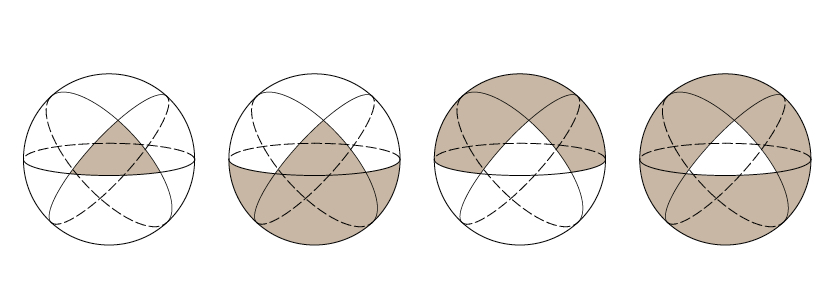
\includegraphics[width=0.9\textwidth]{kugel/Dreieckarten.jpg}
    \captionof{figure}{Dreieckarten auf einer Kugeloberfläche}
\end{center}

Der Begriff Sphärisches Dreieck oder Kugeldreieck ist ein sehr weitläufiger Begriff. 
Dabei können wir den Begriff in drei für uns wesentliche Dreiecke unterteilen:

\begin{itemize}
\item Kugelzweieck
\item Nicht Eulersche’Dreiecke
\item Eulersche’Dreiecke
\end{itemize}

\subsection{Kugelzweieck}

Zwei Grosskreise auf der Kugeloberfläche, zerlegen diese in vier gleiche Kugelzweiecke. 
Jedes dieser Dreieckseiten hat die Länge
$180^{\circ}$ oder $\pi$
Der Flächeninhalt wird dabei nur durch den Winkel $\alpha$ zwischen den beiden Grosskreisen bestimmt.

\begin{center}
        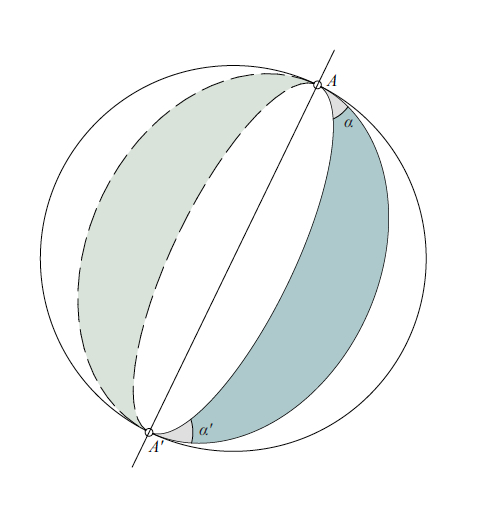
\includegraphics[width=0.3\textwidth]{kugel/Zweieck.jpg}
    \captionof{figure}{Bildung von Zweiecken durch Grosskreise}
\end{center}

Dabei ist der Flächeninhalt der ganzen Kugel:

\begin{align*}
A_{ Kugel } &= 4 \pi r^{2}
\end{align*}


Um den Flächeninhalt des betrachteten Zweieckes zu bekommen, 
müssen wir das ganze noch mit dem Kugelsegment mit dem Winkel $\alpha$ multiplizieren.

\begin{align*}
A_{ Zweieck } &= 4 \pi r^{2} \cdot \frac{ \alpha }{ 2 \pi }
\end{align*}


\subsection{Nicht Eulersche’ Dreiecke}

BLABLA

\subsection{Eulersche’ Dreiecke}

Legt man drei Grosskreise auf eine Kugeloberfläche, bilden sich dabei acht Dreiecke. 
Ein solches Dreieck heisst Eulersches’Dreieck\footnote{%
Leonard Euler (1707-1783), berühmter Schweizer Mathematiker und Physiker. 
Nicht Eulersche’Dreiecke erhält man, indem man das Äussere des Dreieckes ABC betrachtet.} 
Diese Dreiecke werden weder durch die Verlängerung ihrer Seiten durchschnitten, 
noch haben sie Dreiecksseiten welche grösser als $180^{\circ}$ sind.

\begin{center}
        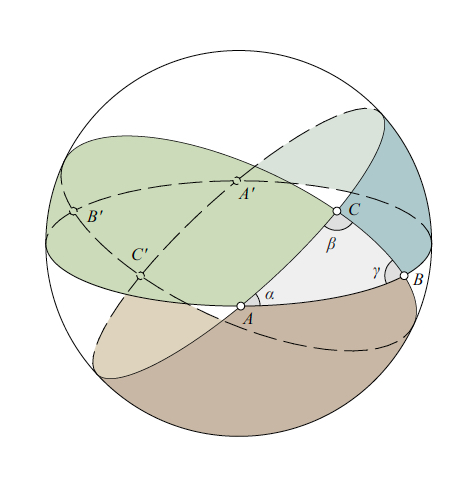
\includegraphics[width=0.4\textwidth]{kugel/Zweiecke.jpg}
    \captionof{figure}{Drei Grosskreise bilden ein sphärisches Dreieck}
\end{center}

In den nachstehenden Erklärungen und Herleitungen, sprechen wir ausschliesslich von Eulerschen’Dreiecken, da die umgeformten Winkelsätze der ebenen Trigonometrie nur auf diese Art von Kugeldreiecken angewendet werden kann.

$A_{ \overline{ ABC }}$ ist die Fläche des Dreieckes auf der Kugeloberfläche
In der ebenen Trigonometrie liegt die Winkelsumme eines Dreiecks bei
$180^{\circ}$.

Anders aber in der sphärischen Trigonometrie. Obschon sie einige Gemeinsamkeiten zur ebenen Trigonometrie aufweist, kann man nicht alles übernehmen.
So auch nicht wie Winkelsumme in einem sphärischen Dreieck.
Diese liegt bei:

\[
\begin{aligned}
\pi
&-
3\pi
&
&\text{\bigg \vert}
&
180^{\circ}
&-
540^{\circ}
\end{aligned}
\]

daraus lässt sich ableiten, das ein einzelner Winkel nicht grösser als $\pi$ oder $180^{\circ}$ sein darf. Ansonsten ist es kein Eulersches’Dreieck und wir dürfen die sphärische Trigonometrie nicht anwenden.\\
Wichtig anzumerken ist, dass die Seiten immer in Radiant beschrieben werden und nicht im Längenmass Meter wie wir es uns gewohnt sind. 
Bei den Dreiecksseiten handelt es sich um Kreisbögen und keine Strecken.

\section{Dreiecksfläche}

\begin{align*}
\text{Zweieck A}
&=
\overline{ABC} + \overline{A'BC} = 2 \alpha r^{ 2 } = A_{ \alpha }\\
\text{Zweieck B}
&=
\overline{ABC} + \overline{AB'C} = 2 \beta r^{ 2 } = A_{ \beta }\\
\text{Zweieck C}
&=
\overline{ABC} + \overline{ABC'} = 2 \gamma r^{ 2 } = A_{ \gamma }
\end{align*}

\begin{align*}
A_{ \alpha } + A_{ \beta } + A_{ \gamma } &= \frac{ 4\pi r^{ 2 } }{ 2 } + 2A_{ \overline{ ABC }} \\
2\alpha r^{ 2 } + 2\beta r^{ 2 } + 2\gamma r^{ 2 } &= \frac{ 4\pi r^{ 2 } }{ 2 } + 2A_{ \overline{ ABC }} \parallel:2\\
\alpha r^{ 2 } + \beta r^{ 2 } + \gamma r^{ 2 } &= \pi r^{ 2 } + A_{ \overline{ ABC }} \parallel-\pi r^{ 2 }\\
r^{ 2 }\left(\alpha + \beta + \gamma - \pi\right) &= A_{ \overline{ ABC }}
\end{align*}




\section{Sphärischer Exzess}
Die Winkelsumme sphärischer Dreiecke ist immer \textgreater \,  $\pi$.

\begin{align*}
\pi < \alpha + \beta + \gamma
\end{align*}

Der sphärische Exzess gibt dabei an, wie stark die Winkelsumme von $\pi$ abweicht.

\begin{align*}
\pi + \epsilon &= \alpha + \beta + \gamma \\
\epsilon &= \alpha + \beta + \gamma - \pi
\end{align*}

Würde der sphärische Exzess in der ebenen Trigonometrie angewendet, wäre dieser = 0. 
Bezieht man das auf die Erde und somit einer Kugel, kann man mit Hilfe eines beliebigen sphärischen Dreieckes und dessen Flächeninhalt auf den Radius der Kugel schliessen.

\subsection{Grenzfall - Satz von Legendre}

\begin{quote} \textit{Ein kleines sphärisches Dreieck kann näherungsweise 
wie ein ebenes Dreieck mit denselben Seiten berechnet 
werden, wenn alle Winkel des ebenen Dreiecks die um 
je ein Drittel des sphärischen Exzesses verminderten 
Winkel des sphärischen Dreiecks nimmt.} \end{quote}
\begin{flushright} - Adrien-Marie Legendre (1752-1833), Paris 1787
\end{flushright}x

Diese Aussage zeigt den Zusammenhang zwischen der 
Trigonometrie in der Ebene sowie in auf der Kugel
auf. Im speziellen bei sehr kleinen sphärischen 
Dreiecken ist die Winkelsumme nur unwesentlich 
grösser als $180^{\circ}$. Des Weiteren kann gesagt werden,
dass der sphärische Exzess gleichmässig auf alle
Winkel aufgeteilt wird.
Wichtig anzumerken ist, dass der Satz von Legendre 
für grosse, aber endliche Radien $r$ gilt.

%[SKIZZE GROSSER RADIUS/KLEINE KRÜMMUNG, KLEINER RADIUS/GROSSE KRÜMMUNG!!!!]
%


\section{Sphärisch Analoge Winkelfunktionen}

\subsection{Sphärischer Sinussatz}

Wir stellen die allgemeinen Sinussätze der Winkel $\alpha$ und $\gamma$ auf:


\[
\begin{aligned}
&{sin(\gamma)} = \frac{h}{a}
&
&\text{\bigg \vert}
&
&{sin(\alpha)} = \frac{h}{c}
&
\end{aligned}
\]

Daraus folgt:
\begin{align*}
h &= sin(\gamma)\cdot a \\
h &= sin(\alpha)\cdot c
\end{align*} 

Durch Gleichsetzung erhält man:
\begin{align*}
h &= h \\
sin(\gamma)\cdot a &= sin(\alpha)\cdot c
\end{align*} 

Durch umstellen erhalten wir den Sinussatz für a und c:
\begin{align*}
sin(\gamma)\cdot a &= sin(\alpha)\cdot c \\
\frac{sin(\gamma)}{c} &= \frac{sin(\alpha)}{a} 
\end{align*} 



\begin{align*}
\frac{sin(\alpha)}{sin(a)} = \frac{sin(\beta)}{sin(b)} = \frac{sin(\gamma)}{sin(c)}
\end{align*} 


\subsection{Winkelkosinussatz}

%[SKIZZE WINKELKOSINUS]

\[
\begin{aligned}
&\overline{C'A'} &= d\cdot {tan(b)}
&
&
&
&
&
&\overline{C'B'} &= d\cdot {tan(a)}
\end{aligned}
\]

\[
\begin{aligned}
&\overline{MA'} &= \frac{ d }{cos(b)}
&
&
&
&
&
&\overline{MB'} &= \frac{ d }{cos(a)}
\end{aligned}
\]

Der allgemeine Kosinussatz beschreibt sich wie folgt:

\begin{align*}
c^{ 2 } &= a^{ 2 } + b^{ 2 } - 2ab \cdot cos(\gamma)
\end{align*}

\begin{align*}
\triangle \overline{A'B'C' }
\overline{ A'B' }^{ 2 } &= \overline{ C'B' }^{ 2 } + \overline{ C'A' }^{ 2 } - 2 \cdot \overline{ C'B' } \cdot \overline{ C'A' } \cdot cos(\gamma)
\end{align*}



\begin{align*}
\overline{A'B'}^{ 2 } &= (d\cdot tan(a))^{ 2 } + (d\cdot tan(b))^{ 2 } - 2 \cdot (d\cdot tan(a) \cdot (d\cdot tan(b) \cdot cos(\gamma)\\
\overline{A'B'}^{ 2 } &= d^{ 2 } \cdot \left(\left(tan^{ 2 }(a) + tan^{ 2 }(b)\right) - 2\cdot tan(a) \cdot tan(b) \cdot cos(\gamma)\right)
\end{align*}

\begin{align*}
\triangle \overline{ MA'B' }
\overline{ A'B' }^{ 2 } &= \overline{ MB' }^{ 2 } + \overline{ MA' }^{ 2 } - 2\cdot \overline{ MB'} \cdot \overline{ MA' } \cdot cos(c)
\end{align*}


\begin{align*}
\overline{ A'B'}^{ 2 } &= \left(\frac{ d }{ cos(a) }  \right)^{ 2 } + \left(\frac{ d }{ cos(b)}  \right)^{ 2 } - 2 \cdot \frac{ d }{ cos(a)} \cdot \frac{ d }{ cos(b)} \cdot cos(c) \\
\overline{ A'B' }^{ 2 } &= d^{ 2 } \cdot \left(\left(\frac{ 1 }{ cos(a) }  \right)^{ 2 } + \left(\frac{ 1 }{ cos(b) }  \right)^{ 2 } - 2 \cdot \frac{ 1 }{ cos(a)} \cdot \frac{ 1 }{ cos(b)} \cdot cos(c)\right)\\
\overline{ A'B' }^{ 2 } &= d^{ 2 } \cdot \left(\left(tan^{ 2 }(a) + 1\right) + \left(tan^{ 2 }(b) + 1\right) - \left(2 \cdot \frac{cos(c)}{cos(a) \cdot cos(b)}\right)\right)
\end{align*}



\begin{align*}
\overline{ A'B'}^{ 2 } &= d^{ 2 } \cdot \left(\left(tan^{ 2 }(a) + tan^{ 2 }(b)\right) - 2 \cdot tan(a) \cdot tan(b) \cdot cos(\gamma)\right) \\
\overline{ A'B'}^{ 2 } &= d^{ 2 } \cdot \left(\left(tan^{ 2 }(a) + 1\right) + \left(tan^{ 2 }(b) + 1\right) - \left(2 \cdot \frac{cos(c)}{cos(a) \cdot cos(b)}\right)\right)
\end{align*}

Die anderen Gleichungen des Satzes, erfolgen aus Symmetriegründen.

\subsection{Seitenkosinussatz}
Durch zyklische Vertauschung des Winkelkosinus erhalten wir den Seitenkosinussatz:

\begin{align*}
{cos(a)} &= {cos(b)} \cdot {cos(c)} + {sin(b)} \cdot {sin(c)} \cdot {sin(\alpha)}\\
{cos(b)} &= {cos(a)} \cdot {cos(c)} + {sin(a)} \cdot {sin(c)} \cdot {sin(\beta)}\\
{cos(c)} &= {cos(a)} \cdot {cos(b)} + {sin(a)} \cdot {sin(b)} \cdot {sin(\gamma)}\\
\end{align*}

\section{Navigation auf See}
Das besondere an Seekarten ist die Inhaltliche Ausrichtung. Anders wie Landkarten muss sie Informationen enthalten welche für den Kapitän und seine Besatzung von grosser Bedeutung sind. Vor allem in Küstennähe ist das navigieren eines Schiffes besonders gefährlich. So enthalten Seekarten etwas über Wassertiefen, Bodenbeschaffenheiten, Gezeiten, Küstenlinien, Landzungen und Windrichtungen.
Der Hauptunterschied dabei ist, das auf der Landkarte feste Positionen definiert und aufgezeigt werden, das einzige was sich verändert ist der Reisende selbst. Bei der Seekarte ist das anders, es werden veränderliche Einwirkungen der Natur festgehalten.

Dieser kleine Unterschied zeigt die Notwendigkeit auf, die Position und den Kurs seines Schiffes auf See immer ermitteln zu können.


\section{Geographische Koordinaten}

Nachdem klar war, das die Erde eine Kugel ist, wurde diese in ein Gradnetz aufgeteilt. Dabei wurden die Angaben für eine exakte Ortsbestimmung klar definiert und die bis heute gültigen Koordinaten bestimmt.
Dabei muss man sich nochmals in Erinnerung rufen, dass sich die Erde in 24h einmal um ihre eigene Achse dreht. Nach $360 ^{\circ}$ 
und somit einer vollen Umdrehung, steht sie wieder in ihrer Ursprungsposition und ein neuer Tag beginnt.

Die Koordinaten setzen sich aus folgenden Komponenten zusammen:

\[
\begin{aligned}
&\text{Grad } (^{\circ})
&
&\text{\bigg \vert}
&
&\text{Bogenminuten } (`)
&
&\text{\bigg \vert}
&
&\text{Bogensekunden } (``)
\end{aligned}
\]

Die Erdoberfläche wurde in je 360 Breiten- und Längengrade eingeteilt. Die Breitengrade haben zueinander einen Abstand von 111.31 km, dies entspricht auch dem Abstand der Längengrade am Äquator mit Zunehmender Nähe zu den Polen, nimmt dieser Abstand ab.

\[
\begin{aligned}
&1^{\circ}
&
&\text{\bigg \vert}
&
&4 \text{ Minuten}
&
&\text{\bigg \vert}
&
&111.31\text{ km}
\end{aligned}
\]

Berechnet man nun die Erdumdrehung von 360°, erhält man genau den Erdumfang am Äquator: \begin{align*} 40’074 \text{ km.}\end{align*}

Dabei geben die Bogenminuten und -sekunden dem Standort die gewünschte Exaktheit. Mit den vollständigen Koordinaten lässt sich der Standort auf einer Landkarte exakt bestimmen und einzeichnen.

\subsection{Zeitzonen der Erde}
Wenn man nun die verschiedenen Zeitzonen der Erde betrachtet, macht die Verschiebung von jeweils einer Stunde durchaus Sinn, es lässt sich auf die Längengrade schliessen.
Zwischen den verschiedenen Zeitzonen liegen 15 Längengrade:

\begin{align*}
\text{15 Längengrade à 4 Minuten = 60 Minuten Zeitverschiebung = ca. 1665 km}
\end{align*}

Dabei ist die Zeitzone in welcher Mitte sich der Greenwich Meredian befindet die \textit{Greenwich Mean Time (GMT)} welche bis 1928 als Weltzeit galt. Im Jahr 1972 wurde diese umbenannt in die \textit{Coordinated Universal Time (UTC)} und wir von da an als Weltzeit $\pm$ 0.00 verwendet.


\section{Der Breitengrad}
Die Breitengrade bilden die bereits genannten Kleinkreise auf der Kugeloberfläche. Sie verlaufen in einem Abstand von genau 111 km parallel zum Äquator. Dabei stellt  dieser genau die Mitte zwischen Nord- und Südpol dar und teilt die Erdkugel in zwei gleiche Hälften. Somit wird von nördlicher und südlicher Breite gesprochen, je nach dem auf welcher Halbkugel man sich befindet.

%[SKIZZE DER GEOGRAFISCHEN BREITE ERDKUGEL]

\subsection{Geografische Breite $\phi$}
\begin{definition}
Die geografische Breite eines Standortes ist nichts anderes, als der Winkel am Erdmittelpunkt zwischen der Ebene des Äquators und der Geraden zum Standpunkt auf der Erdoberfläche.
\end{definition}

%[SKIZZE DER GEOGRAFISCHEN BREITE MIT WINKEL]

\subsection{Navigation mit den Breitengraden}
Da der Breitengrad bereits sehr früh ziemlich präzise bestimmt werden könnte, nutzten bereits die Seefahrer um Christoph Kolumbus den Breitengrad zur Navigation ihrer Flotten.
Den dieser lässt sich ziemlich einfach aus dem höchsten Sonnenstand oder einem Fixstern bestimmen. Dabei wird mit einem Jakobsstab\footnote{%
Der Jakobsstab ist ein früheres astronomisches Instrument zur Winkelmessung und wurde vor allem in der Seefahrt verwendet. Er ist in der Nautik der Vorläufer des Sextanten.} (später Sextant\footnote{%
Der Sextant ist ein nautisches Messinstrument zur Winkelmessung von Horizont und Fixstern (Gestirn)}) der Winkel zwischen dem Horizont und dem Fixstern gemessen. Der Winkel welchen man erhält, zieht man von 90° ab und erhält somit die geografische Breite. \\

%[SKIZZE ERMITTLUNG DES BREITENGRADES]

Wenn man sich auf der Nordhalbkugel befindet, ist der Polarstern ein sehr guter Fixstern. Befindet sich ein Schiff nun sehr nahe am Nordpol, steht dieser nahezu senkrecht am Himmelszelt bei $90^{\circ}$. Würde es aber nahe dem Äquator stehen, erscheint dieser am Horizont bei $0^{\circ}$.

\subsection{Korrekturbeiwert}

\section{Der Längengrad}
Die Längengrade bilden die bereits genannten Grosskreise auf der Kugeloberfläche.
Sie schneiden den Äquator im rechten Winkel, haben dort einen Abstand von 111 km zueinander und verbinden die Pole. Anders wie bei der geografischen Breite, ist in der Natur kein Längengrad gegeben welcher den Nullpunkt darstellt.

%[SKIZZE DER GEOGRAFISCHEN LÄNGE ERDKUGEL]

\subsection{Geografische Länge $\lambda$}
\begin{definition}
Die geografische Länge ist der Winkel an der Erdachse zum Nullmeridian.
\end{definition}

\subsection{Navigation mit den Längengraden}
Die geografische Länge lässt sich nicht so einfach bestimmen wie deren Breite. Für die Berechnung auf See benötigt man eine Referenzzeit eines Ortes mit bekannter Länge.
In der Zeit der Entdecker gab es noch keine mechanischen Uhren. Die Sonnenuhr war zudem ungeeignet, da diese nur die Uhrzeit am Standort mass und nicht die am Referenzort selbst. Die erste Pendeluhr wurde erst Mitte des 17. Jahrhunderts erfunden, was in der Schifffahrt aber auch nicht die Lösung brachte.\\
Pendeluhren auf einem Schiff sind ungeeignet, da das Pendel mit dem Wellengang aus dem Takt gebracht wird und somit die Uhr falsch geht.
Zu ungenau und gegen äussere Erschütterungen zu empfindlich waren später auch die federgetriebenen Uhren und die Unruh. Dazukamen die verschiedenen Klimazonen welche ein Schiff zu durchqueren hatten. Das Metall zog sich viel zu fest zusammen oder dehnte sich aus, was dazu führte das die Uhr unregelmässig lief.

Das sogenannte „Längenproblem“ stellte nicht nur bei der Navigation auf See ein Problem dar, es ergaben sich auch wirtschaftliche Konsequenzen. Die Schiffe mussten bis zur gewünschten geografischen Breite navigieren und segelten dann den Breitengrad entlang. Dabei waren die Schiffe oft Wochenlang unterwegs und segelten die „Breiten ab“ um an die gewünschte Position zu kommen. Dies führte zu erheblichen Zeitverlusten und viel längeren Reisezeiten.


\section{The Board of Longitude - Das Längenproblem}
Das Längenproblem beschäftigte alle grossen Seefahrernationen Europas. Wenn man bedenkt das sich Werte in einer  Höhe von halben britischen Staatshaushalten auf verloren gegangenen Schiffen befanden, erkennt man die Dringlichkeit für eine zuverlässige und genaue Navigation auf See.


\begin{itemize}
\item £ 20’000 - Abweichung von max. einem halben Grad
\item £ 15’000 - Abweichung von zwei Drittel Grad
\item £ 10’000 - Abweichung von max. $1 ^{\circ}$
\end{itemize}

\subsection{John Harrison}


\subsection{Tobias Mayer}



Uhren mit einer Abweichung von einer Minute Abweichung pro Tag (





\section{Nautische Dreieck}


$\Rightarrow$





\section{Die Vermessung der Welt}
Wir schreiben das Jahr 1818 und kehren in die Zeit des Mathematikers Carl Friedrich Gauss zurück. Neben dem liebevoll genannten „kleinen Gauss“ und anderen herausragenden Mathematischen Leistungen, beschäftigte er in den Folgejahren mit der Vermessung des Königreichs Hannovers und verfasste auf 61 Blättern das Kartenwerk \textit{Gauss’sche Landesaufnahme der 1815 durch Hannover erworbenen Gebiete}.






AUFGABE

Hubble Teleskop 
24. April 1990






\printbibliography[heading=subbibliography]
\end{refsection}




%\chapter{Geometrie auf der Kugeloberfläche\label{chapter:kugel}}
\lhead{Geometrie auf der Kugeloberfläche}
\begin{refsection}
\chapterauthor{Melina Staub und Fabian Schmid}

\section{Einleitung}

Schon seit jeher fasziniert den Menschen die Fahrt zur See. Nicht grundlos ist die Seefahrt eine der wichtigsten und ältesten Tätigkeiten der Menschheit. Der innerliche Drang neue Weltmeere und unbekannte Gebiete zu entdecken, die Fahrt zur See zu erleichtern und erträglicher zu machen, trieben die Menschen an, die Schiffe dieser Welt immer weiter zu entwickeln.

Die Idee der Kugelform der Erde ist älter als man zu denken vermag. Bereits der Schüler des antiken griechischen Philosophen Platon - Aristoteles schrieb in seiner Schrift \textit{Über den Himmel} aus dem 4. Jahrhundert v. Chr. etliche Gründe welche für die Gestallt der Erde als Kugel sprechen:

\begin{itemize}
      \item Sämtliche schweren Körper streben zum Mittelpunkt des Alls. Da sie dies von allen Seiten her gleichmäßig tun und die Erde im Mittelpunkt des Alls steht, muss sie eine kugelrunde Gestalt annehmen. 
\item Bei von der Küste wegfahrende Schiffen wird der Rumpf vor den Segeln der Sicht verborgen. 
\item In südlichen Ländern erscheinen südliche Sternbilder höher über dem Horizont.
\item Der Erdschatten bei einer Mondfinsternis ist stets rund.
\end{itemize}

Jedoch war um 1492 - der Zeit der Entdeckung Amerikas durch Christoph Kolumbus, die Idee der Erde in Kugelform noch sehr umstritten. Er erkannte anhand den Theorien und Erkenntnissen der alten Griechen, vor allem Aristoteles, das die Erde eine Kugel sein muss. \\
Doch mit seinem Vorschlag einen Seeweg über den Atlantik nach Indien zu finden und nicht wie üblich um Afrika zu segeln, stiess er beim beim portugiesischen König auf taube Ohren. Sein Plan Indien über eine Route nach Westen zu erreichen, widersprach dem gesunden Menschenverstand. Wäre die Erde wirklich eine Kugel und man befände sich auf der unteren Erdhalbkugel, würde man herunterfallen.\\
Doch auch der damals übliche Glaube an die Erde in Scheibenform brachte so einige Risiken mit sich. Was würde passieren, wenn die Flotte das Ende der Scheibe erreicht hatte? Würden sie über den Erdrand hinweggleiten und in den Abgrund stürzen?\\
Erst nach viel Überzeugungsarbeit durch Kolumbus, setzte er sich am Spanischen Hof durch und segelte über die Westliche Route über den Atlantik und entdeckte schlussendlich Amerika.

Der praktische und greifbare Beweis das die Erde eine Kugel ist, lieferte rund 30 Jahre später der Portugiese Fernando Magellan. Mit seiner Weltumsegelung und seiner Ankunft in den Philippinen, bewies er definitiv das die Erde eine Kugel ist.\\

Nun wollen wir uns die Frage stellen, wie die alten Seefahrer ohne GPS und jeglichen modernen Navigationssystemen auf hoher See wussten wo sie sich befinden und was haben die Sterne mit alldem zu tun? Reisen Sie mit uns zurück in eine Zeit mit Sextant, Kompass und Sternkarten. In die Zeit der Seefahrer und Entdecker.


\section{Geometrie auf der Ebene und der Kugel}

Euklid von Alexandria beschrieb die Grundbegriffe der ebenen Geometrie mittels Punkt, Geraden, Ebene, Winkel und Dreieck. Diese Dreiecke lassen sich mithilfe der ebenen Trigonometrie beschreiben. Dabei gelten die uns bekannten trigonometrischen Winkelfunktionen:\\

\text{Sinussatz:}
\begin{align*}
\frac{ a }{ sin(\alpha) } &= \frac{ b }{sin(\beta)} = \frac{ c }{ sin(\gamma) } = \frac{abc}{2A} = 2r\\
\end{align*}

\text{Cosinussatz:}
\begin{align*}
c^{ 2 } &= a^{ 2 } + b^{ 2 } - 2ab\cdot cos(\gamma)\\
b^{ 2 } &= a^{ 2 } + c^{ 2 } - 2ab\cdot cos(\beta)\\
a^{ 2 } &= b^{ 2 } + c^{ 2 } - 2ab\cdot cos(\alpha)
\end{align*}

Um Dreiecke auf der Kugeloberfläche zu berechnen, benötigt man die sphärische Trigonometrie. Die oben beschriebenen Sätze lassen sich auf der Kugel nicht anwenden, sie werden aber als Grundlage zur Herleitung der Sätze für das Kugeldreieck benötigt.

Die nachfolgenden Seiten thematisieren die Geometrie auf der Kugeloberfläche und wie sie in der Navigation eingesetzt werden kann.


\section{Gross- und Kleinkreise}

Eine Kugeloberfläche lässt sich in zwei verschiedene Kreisarten einteilen -  Gross- und Kleinkreise. 
Wir betrachten als erstes die Grosskreise:

\begin{definition}
Ein Großkreis ist ein größtmöglicher Kreis auf einer Kugeloberfläche. Sein Mittelpunkt fällt immer mit dem Mittelpunkt der Kugel zusammen und ein Schnitt auf dem Großkreis teilt die Kugel in jedem Fall in zwei („gleich große“) Hälften.
\end{definition}

Es gibt unendlich viele Möglichkeiten, eine Kugel in zwei gleich grosse Stücke zu zerschneiden, 
daher gibt es auch unendlich viele Grosskreise. Wenn wir die Grosskreise auf einer Kugel mit diesen auf der Erde beschreiben, sprechen wir von den Längengraden aber auch der Äquator beschreibt einen Grosskreis.
Ein Elementarer Bestandteil bilden die Grosskreise in der sphärischen Trigonometrie. Mithilfe der Schnittpunkte verschiedener Grosskreise, lässt sich ein Sphärisches Dreieck bilden auf welchem sich die sphärische Trigonometrie anwenden lässt.

[GRAFIK GROSSKREISE]

\begin{definition}
Unter Kleinkreis versteht man jene Kreise auf einer Kugeloberfläche, deren Ebenen nicht den Kugelmittelpunkt enthalten.
\end{definition}

Die Kleinkreise eignen sich im Gegensatz zu den Grosskreisen \textit{nicht} für die sphärische Trigonometrie. 
Sie werden lediglich zur Bestimmung der Messgrössen, Winkelabstände oder des Höhenwinkels eines Gestirns verwendet. 

Wenn wir die Kleinkreise auf die Erdoberfläche projizieren betrachten wir die Breitengrade.

[GRAFIK KLEINKREISE]


\section{Sphärische Dreiecke / Kugeldreieck}

\begin{center}
        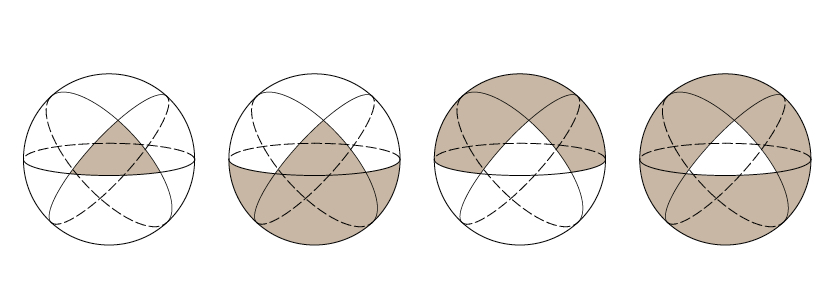
\includegraphics[width=0.9\textwidth]{kugel/Dreieckarten.jpg}
    \captionof{figure}{Dreieckarten auf einer Kugeloberfläche}
\end{center}

Der Begriff Sphärisches Dreieck oder Kugeldreieck ist ein sehr weitläufiger Begriff. 
Dabei können wir den Begriff in drei für uns wesentliche Dreiecke unterteilen:

\begin{itemize}
\item Kugelzweieck
\item Nicht Eulersche’Dreiecke
\item Eulersche’Dreiecke
\end{itemize}

\subsection{Kugelzweieck}

Zwei Grosskreise auf der Kugeloberfläche, zerlegen diese in vier gleiche Kugelzweiecke. 
Jedes dieser Dreieckseiten hat die Länge
$180^{\circ}$ oder $\pi$
Der Flächeninhalt wird dabei nur durch den Winkel $\alpha$ zwischen den beiden Grosskreisen bestimmt.

\begin{center}
        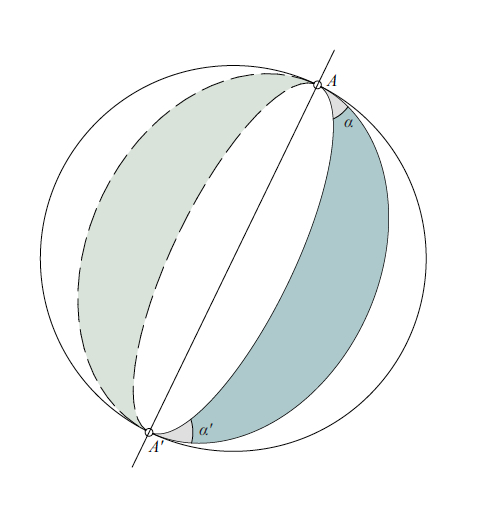
\includegraphics[width=0.3\textwidth]{kugel/Zweieck.jpg}
    \captionof{figure}{Bildung von Zweiecken durch Grosskreise}
\end{center}

Dabei ist der Flächeninhalt der ganzen Kugel:

\begin{align*}
A_{ Kugel } &= 4 \pi r^{2}
\end{align*}


Um den Flächeninhalt des betrachteten Zweieckes zu bekommen, 
müssen wir das ganze noch mit dem Kugelsegment mit dem Winkel $\alpha$ multiplizieren.

\begin{align*}
A_{ Zweieck } &= 4 \pi r^{2} \cdot \frac{ \alpha }{ 2 \pi }
\end{align*}


\subsection{Nicht Eulersche’ Dreiecke}

BLABLA

\subsection{Eulersche’ Dreiecke}

Legt man drei Grosskreise auf eine Kugeloberfläche, bilden sich dabei acht Dreiecke. 
Ein solches Dreieck heisst Eulersches’Dreieck\footnote{%
Leonard Euler (1707-1783), berühmter Schweizer Mathematiker und Physiker. 
Nicht Eulersche’Dreiecke erhält man, indem man das Äussere des Dreieckes ABC betrachtet.} 
Diese Dreiecke werden weder durch die Verlängerung ihrer Seiten durchschnitten, 
noch haben sie Dreiecksseiten welche grösser als $180^{\circ}$ sind.

\begin{center}
        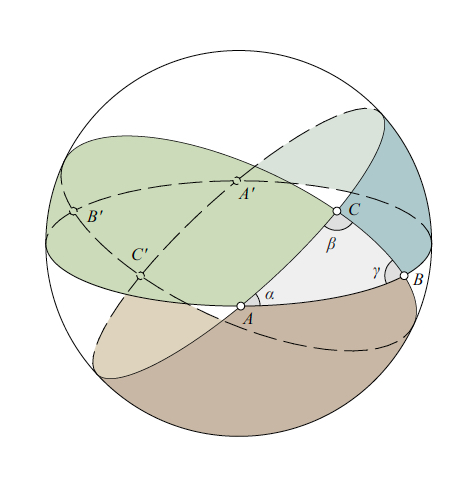
\includegraphics[width=0.4\textwidth]{kugel/Zweiecke.jpg}
    \captionof{figure}{Drei Grosskreise bilden ein sphärisches Dreieck}
\end{center}

In den nachstehenden Erklärungen und Herleitungen, sprechen wir ausschliesslich von Eulerschen’Dreiecken, da die umgeformten Winkelsätze der ebenen Trigonometrie nur auf diese Art von Kugeldreiecken angewendet werden kann.

$A_{ \overline{ ABC }}$ ist die Fläche des Dreieckes auf der Kugeloberfläche
In der ebenen Trigonometrie liegt die Winkelsumme eines Dreiecks bei
$180^{\circ}$.

Anders aber in der sphärischen Trigonometrie. Obschon sie einige Gemeinsamkeiten zur ebenen Trigonometrie aufweist, kann man nicht alles übernehmen.
So auch nicht wie Winkelsumme in einem sphärischen Dreieck.
Diese liegt bei:

\[
\begin{aligned}
\pi
&-
3\pi
&
&\text{\bigg \vert}
&
180^{\circ}
&-
540^{\circ}
\end{aligned}
\]

daraus lässt sich ableiten, das ein einzelner Winkel nicht grösser als $\pi$ oder $180^{\circ}$ sein darf. Ansonsten ist es kein Eulersches’Dreieck und wir dürfen die sphärische Trigonometrie nicht anwenden.\\
Wichtig anzumerken ist, dass die Seiten immer in Radiant beschrieben werden und nicht im Längenmass Meter wie wir es uns gewohnt sind. 
Bei den Dreiecksseiten handelt es sich um Kreisbögen und keine Strecken.

\section{Dreiecksfläche}

\begin{align*}
\text{Zweieck A}
&=
\overline{ABC} + \overline{A'BC} = 2 \alpha r^{ 2 } = A_{ \alpha }\\
\text{Zweieck B}
&=
\overline{ABC} + \overline{AB'C} = 2 \beta r^{ 2 } = A_{ \beta }\\
\text{Zweieck C}
&=
\overline{ABC} + \overline{ABC'} = 2 \gamma r^{ 2 } = A_{ \gamma }
\end{align*}

\begin{align*}
A_{ \alpha } + A_{ \beta } + A_{ \gamma } &= \frac{ 4\pi r^{ 2 } }{ 2 } + 2A_{ \overline{ ABC }} \\
2\alpha r^{ 2 } + 2\beta r^{ 2 } + 2\gamma r^{ 2 } &= \frac{ 4\pi r^{ 2 } }{ 2 } + 2A_{ \overline{ ABC }} \parallel:2\\
\alpha r^{ 2 } + \beta r^{ 2 } + \gamma r^{ 2 } &= \pi r^{ 2 } + A_{ \overline{ ABC }} \parallel-\pi r^{ 2 }\\
r^{ 2 }\left(\alpha + \beta + \gamma - \pi\right) &= A_{ \overline{ ABC }}
\end{align*}




\section{Sphärischer Exzess}
Die Winkelsumme sphärischer Dreiecke ist immer \textgreater \,  $\pi$.

\begin{align*}
\pi < \alpha + \beta + \gamma
\end{align*}

Der sphärische Exzess gibt dabei an, wie stark die Winkelsumme von $\pi$ abweicht.

\begin{align*}
\pi + \epsilon &= \alpha + \beta + \gamma \\
\epsilon &= \alpha + \beta + \gamma - \pi
\end{align*}

Würde der sphärische Exzess in der ebenen Trigonometrie angewendet, wäre dieser = 0. 
Bezieht man das auf die Erde und somit einer Kugel, kann man mit Hilfe eines beliebigen sphärischen Dreieckes und dessen Flächeninhalt auf den Radius der Kugel schliessen.

\subsection{Grenzfall - Satz von Legendre}

\begin{quote} \textit{Ein kleines sphärisches Dreieck kann näherungsweise 
wie ein ebenes Dreieck mit denselben Seiten berechnet 
werden, wenn alle Winkel des ebenen Dreiecks die um 
je ein Drittel des sphärischen Exzesses verminderten 
Winkel des sphärischen Dreiecks nimmt.} \end{quote}
\begin{flushright} - Adrien-Marie Legendre (1752-1833), Paris 1787
\end{flushright}x

Diese Aussage zeigt den Zusammenhang zwischen der 
Trigonometrie in der Ebene sowie in auf der Kugel
auf. Im speziellen bei sehr kleinen sphärischen 
Dreiecken ist die Winkelsumme nur unwesentlich 
grösser als $180^{\circ}$. Des Weiteren kann gesagt werden,
dass der sphärische Exzess gleichmässig auf alle
Winkel aufgeteilt wird.
Wichtig anzumerken ist, dass der Satz von Legendre 
für grosse, aber endliche Radien $r$ gilt.

%[SKIZZE GROSSER RADIUS/KLEINE KRÜMMUNG, KLEINER RADIUS/GROSSE KRÜMMUNG!!!!]
%


\section{Sphärisch Analoge Winkelfunktionen}

\subsection{Sphärischer Sinussatz}

Wir stellen die allgemeinen Sinussätze der Winkel $\alpha$ und $\gamma$ auf:


\[
\begin{aligned}
&{sin(\gamma)} = \frac{h}{a}
&
&\text{\bigg \vert}
&
&{sin(\alpha)} = \frac{h}{c}
&
\end{aligned}
\]

Daraus folgt:
\begin{align*}
h &= sin(\gamma)\cdot a \\
h &= sin(\alpha)\cdot c
\end{align*} 

Durch Gleichsetzung erhält man:
\begin{align*}
h &= h \\
sin(\gamma)\cdot a &= sin(\alpha)\cdot c
\end{align*} 

Durch umstellen erhalten wir den Sinussatz für a und c:
\begin{align*}
sin(\gamma)\cdot a &= sin(\alpha)\cdot c \\
\frac{sin(\gamma)}{c} &= \frac{sin(\alpha)}{a} 
\end{align*} 



\begin{align*}
\frac{sin(\alpha)}{sin(a)} = \frac{sin(\beta)}{sin(b)} = \frac{sin(\gamma)}{sin(c)}
\end{align*} 


\subsection{Winkelkosinussatz}

%[SKIZZE WINKELKOSINUS]

\[
\begin{aligned}
&\overline{C'A'} &= d\cdot {tan(b)}
&
&
&
&
&
&\overline{C'B'} &= d\cdot {tan(a)}
\end{aligned}
\]

\[
\begin{aligned}
&\overline{MA'} &= \frac{ d }{cos(b)}
&
&
&
&
&
&\overline{MB'} &= \frac{ d }{cos(a)}
\end{aligned}
\]

Der allgemeine Kosinussatz beschreibt sich wie folgt:

\begin{align*}
c^{ 2 } &= a^{ 2 } + b^{ 2 } - 2ab \cdot cos(\gamma)
\end{align*}

\begin{align*}
\triangle \overline{A'B'C' }
\overline{ A'B' }^{ 2 } &= \overline{ C'B' }^{ 2 } + \overline{ C'A' }^{ 2 } - 2 \cdot \overline{ C'B' } \cdot \overline{ C'A' } \cdot cos(\gamma)
\end{align*}



\begin{align*}
\overline{A'B'}^{ 2 } &= (d\cdot tan(a))^{ 2 } + (d\cdot tan(b))^{ 2 } - 2 \cdot (d\cdot tan(a) \cdot (d\cdot tan(b) \cdot cos(\gamma)\\
\overline{A'B'}^{ 2 } &= d^{ 2 } \cdot \left(\left(tan^{ 2 }(a) + tan^{ 2 }(b)\right) - 2\cdot tan(a) \cdot tan(b) \cdot cos(\gamma)\right)
\end{align*}

\begin{align*}
\triangle \overline{ MA'B' }
\overline{ A'B' }^{ 2 } &= \overline{ MB' }^{ 2 } + \overline{ MA' }^{ 2 } - 2\cdot \overline{ MB'} \cdot \overline{ MA' } \cdot cos(c)
\end{align*}


\begin{align*}
\overline{ A'B'}^{ 2 } &= \left(\frac{ d }{ cos(a) }  \right)^{ 2 } + \left(\frac{ d }{ cos(b)}  \right)^{ 2 } - 2 \cdot \frac{ d }{ cos(a)} \cdot \frac{ d }{ cos(b)} \cdot cos(c) \\
\overline{ A'B' }^{ 2 } &= d^{ 2 } \cdot \left(\left(\frac{ 1 }{ cos(a) }  \right)^{ 2 } + \left(\frac{ 1 }{ cos(b) }  \right)^{ 2 } - 2 \cdot \frac{ 1 }{ cos(a)} \cdot \frac{ 1 }{ cos(b)} \cdot cos(c)\right)\\
\overline{ A'B' }^{ 2 } &= d^{ 2 } \cdot \left(\left(tan^{ 2 }(a) + 1\right) + \left(tan^{ 2 }(b) + 1\right) - \left(2 \cdot \frac{cos(c)}{cos(a) \cdot cos(b)}\right)\right)
\end{align*}



\begin{align*}
\overline{ A'B'}^{ 2 } &= d^{ 2 } \cdot \left(\left(tan^{ 2 }(a) + tan^{ 2 }(b)\right) - 2 \cdot tan(a) \cdot tan(b) \cdot cos(\gamma)\right) \\
\overline{ A'B'}^{ 2 } &= d^{ 2 } \cdot \left(\left(tan^{ 2 }(a) + 1\right) + \left(tan^{ 2 }(b) + 1\right) - \left(2 \cdot \frac{cos(c)}{cos(a) \cdot cos(b)}\right)\right)
\end{align*}

Die anderen Gleichungen des Satzes, erfolgen aus Symmetriegründen.

\subsection{Seitenkosinussatz}
Durch zyklische Vertauschung des Winkelkosinus erhalten wir den Seitenkosinussatz:

\begin{align*}
{cos(a)} &= {cos(b)} \cdot {cos(c)} + {sin(b)} \cdot {sin(c)} \cdot {sin(\alpha)}\\
{cos(b)} &= {cos(a)} \cdot {cos(c)} + {sin(a)} \cdot {sin(c)} \cdot {sin(\beta)}\\
{cos(c)} &= {cos(a)} \cdot {cos(b)} + {sin(a)} \cdot {sin(b)} \cdot {sin(\gamma)}\\
\end{align*}

\section{Navigation auf See}
Das besondere an Seekarten ist die Inhaltliche Ausrichtung. Anders wie Landkarten muss sie Informationen enthalten welche für den Kapitän und seine Besatzung von grosser Bedeutung sind. Vor allem in Küstennähe ist das navigieren eines Schiffes besonders gefährlich. So enthalten Seekarten etwas über Wassertiefen, Bodenbeschaffenheiten, Gezeiten, Küstenlinien, Landzungen und Windrichtungen.
Der Hauptunterschied dabei ist, das auf der Landkarte feste Positionen definiert und aufgezeigt werden, das einzige was sich verändert ist der Reisende selbst. Bei der Seekarte ist das anders, es werden veränderliche Einwirkungen der Natur festgehalten.

Dieser kleine Unterschied zeigt die Notwendigkeit auf, die Position und den Kurs seines Schiffes auf See immer ermitteln zu können.


\section{Geographische Koordinaten}

Nachdem klar war, das die Erde eine Kugel ist, wurde diese in ein Gradnetz aufgeteilt. Dabei wurden die Angaben für eine exakte Ortsbestimmung klar definiert und die bis heute gültigen Koordinaten bestimmt.
Dabei muss man sich nochmals in Erinnerung rufen, dass sich die Erde in 24h einmal um ihre eigene Achse dreht. Nach $360 ^{\circ}$ 
und somit einer vollen Umdrehung, steht sie wieder in ihrer Ursprungsposition und ein neuer Tag beginnt.

Die Koordinaten setzen sich aus folgenden Komponenten zusammen:

\[
\begin{aligned}
&\text{Grad } (^{\circ})
&
&\text{\bigg \vert}
&
&\text{Bogenminuten } (`)
&
&\text{\bigg \vert}
&
&\text{Bogensekunden } (``)
\end{aligned}
\]

Die Erdoberfläche wurde in je 360 Breiten- und Längengrade eingeteilt. Die Breitengrade haben zueinander einen Abstand von 111.31 km, dies entspricht auch dem Abstand der Längengrade am Äquator mit Zunehmender Nähe zu den Polen, nimmt dieser Abstand ab.

\[
\begin{aligned}
&1^{\circ}
&
&\text{\bigg \vert}
&
&4 \text{ Minuten}
&
&\text{\bigg \vert}
&
&111.31\text{ km}
\end{aligned}
\]

Berechnet man nun die Erdumdrehung von 360°, erhält man genau den Erdumfang am Äquator: \begin{align*} 40’074 \text{ km.}\end{align*}

Dabei geben die Bogenminuten und -sekunden dem Standort die gewünschte Exaktheit. Mit den vollständigen Koordinaten lässt sich der Standort auf einer Landkarte exakt bestimmen und einzeichnen.

\subsection{Zeitzonen der Erde}
Wenn man nun die verschiedenen Zeitzonen der Erde betrachtet, macht die Verschiebung von jeweils einer Stunde durchaus Sinn, es lässt sich auf die Längengrade schliessen.
Zwischen den verschiedenen Zeitzonen liegen 15 Längengrade:

\begin{align*}
\text{15 Längengrade à 4 Minuten = 60 Minuten Zeitverschiebung = ca. 1665 km}
\end{align*}

Dabei ist die Zeitzone in welcher Mitte sich der Greenwich Meredian befindet die \textit{Greenwich Mean Time (GMT)} welche bis 1928 als Weltzeit galt. Im Jahr 1972 wurde diese umbenannt in die \textit{Coordinated Universal Time (UTC)} und wir von da an als Weltzeit $\pm$ 0.00 verwendet.


\section{Der Breitengrad}
Die Breitengrade bilden die bereits genannten Kleinkreise auf der Kugeloberfläche. Sie verlaufen in einem Abstand von genau 111 km parallel zum Äquator. Dabei stellt  dieser genau die Mitte zwischen Nord- und Südpol dar und teilt die Erdkugel in zwei gleiche Hälften. Somit wird von nördlicher und südlicher Breite gesprochen, je nach dem auf welcher Halbkugel man sich befindet.

%[SKIZZE DER GEOGRAFISCHEN BREITE ERDKUGEL]

\subsection{Geografische Breite $\phi$}
\begin{definition}
Die geografische Breite eines Standortes ist nichts anderes, als der Winkel am Erdmittelpunkt zwischen der Ebene des Äquators und der Geraden zum Standpunkt auf der Erdoberfläche.
\end{definition}

%[SKIZZE DER GEOGRAFISCHEN BREITE MIT WINKEL]

\subsection{Navigation mit den Breitengraden}
Da der Breitengrad bereits sehr früh ziemlich präzise bestimmt werden könnte, nutzten bereits die Seefahrer um Christoph Kolumbus den Breitengrad zur Navigation ihrer Flotten.
Den dieser lässt sich ziemlich einfach aus dem höchsten Sonnenstand oder einem Fixstern bestimmen. Dabei wird mit einem Jakobsstab\footnote{%
Der Jakobsstab ist ein früheres astronomisches Instrument zur Winkelmessung und wurde vor allem in der Seefahrt verwendet. Er ist in der Nautik der Vorläufer des Sextanten.} (später Sextant\footnote{%
Der Sextant ist ein nautisches Messinstrument zur Winkelmessung von Horizont und Fixstern (Gestirn)}) der Winkel zwischen dem Horizont und dem Fixstern gemessen. Der Winkel welchen man erhält, zieht man von 90° ab und erhält somit die geografische Breite. \\

%[SKIZZE ERMITTLUNG DES BREITENGRADES]

Wenn man sich auf der Nordhalbkugel befindet, ist der Polarstern ein sehr guter Fixstern. Befindet sich ein Schiff nun sehr nahe am Nordpol, steht dieser nahezu senkrecht am Himmelszelt bei $90^{\circ}$. Würde es aber nahe dem Äquator stehen, erscheint dieser am Horizont bei $0^{\circ}$.

\subsection{Korrekturbeiwert}

\section{Der Längengrad}
Die Längengrade bilden die bereits genannten Grosskreise auf der Kugeloberfläche.
Sie schneiden den Äquator im rechten Winkel, haben dort einen Abstand von 111 km zueinander und verbinden die Pole. Anders wie bei der geografischen Breite, ist in der Natur kein Längengrad gegeben welcher den Nullpunkt darstellt.

%[SKIZZE DER GEOGRAFISCHEN LÄNGE ERDKUGEL]

\subsection{Geografische Länge $\lambda$}
\begin{definition}
Die geografische Länge ist der Winkel an der Erdachse zum Nullmeridian.
\end{definition}

\subsection{Navigation mit den Längengraden}
Die geografische Länge lässt sich nicht so einfach bestimmen wie deren Breite. Für die Berechnung auf See benötigt man eine Referenzzeit eines Ortes mit bekannter Länge.
In der Zeit der Entdecker gab es noch keine mechanischen Uhren. Die Sonnenuhr war zudem ungeeignet, da diese nur die Uhrzeit am Standort mass und nicht die am Referenzort selbst. Die erste Pendeluhr wurde erst Mitte des 17. Jahrhunderts erfunden, was in der Schifffahrt aber auch nicht die Lösung brachte.\\
Pendeluhren auf einem Schiff sind ungeeignet, da das Pendel mit dem Wellengang aus dem Takt gebracht wird und somit die Uhr falsch geht.
Zu ungenau und gegen äussere Erschütterungen zu empfindlich waren später auch die federgetriebenen Uhren und die Unruh. Dazukamen die verschiedenen Klimazonen welche ein Schiff zu durchqueren hatten. Das Metall zog sich viel zu fest zusammen oder dehnte sich aus, was dazu führte das die Uhr unregelmässig lief.

Das sogenannte „Längenproblem“ stellte nicht nur bei der Navigation auf See ein Problem dar, es ergaben sich auch wirtschaftliche Konsequenzen. Die Schiffe mussten bis zur gewünschten geografischen Breite navigieren und segelten dann den Breitengrad entlang. Dabei waren die Schiffe oft Wochenlang unterwegs und segelten die „Breiten ab“ um an die gewünschte Position zu kommen. Dies führte zu erheblichen Zeitverlusten und viel längeren Reisezeiten.


\section{The Board of Longitude - Das Längenproblem}
Das Längenproblem beschäftigte alle grossen Seefahrernationen Europas. Wenn man bedenkt das sich Werte in einer  Höhe von halben britischen Staatshaushalten auf verloren gegangenen Schiffen befanden, erkennt man die Dringlichkeit für eine zuverlässige und genaue Navigation auf See.


\begin{itemize}
\item £ 20’000 - Abweichung von max. einem halben Grad
\item £ 15’000 - Abweichung von zwei Drittel Grad
\item £ 10’000 - Abweichung von max. $1 ^{\circ}$
\end{itemize}

\subsection{John Harrison}


\subsection{Tobias Mayer}



Uhren mit einer Abweichung von einer Minute Abweichung pro Tag (





\section{Nautische Dreieck}


$\Rightarrow$





\section{Die Vermessung der Welt}
Wir schreiben das Jahr 1818 und kehren in die Zeit des Mathematikers Carl Friedrich Gauss zurück. Neben dem liebevoll genannten „kleinen Gauss“ und anderen herausragenden Mathematischen Leistungen, beschäftigte er in den Folgejahren mit der Vermessung des Königreichs Hannovers und verfasste auf 61 Blättern das Kartenwerk \textit{Gauss’sche Landesaufnahme der 1815 durch Hannover erworbenen Gebiete}.






AUFGABE

Hubble Teleskop 
24. April 1990






\printbibliography[heading=subbibliography]
\end{refsection}




%\chapter{Geometrie auf der Kugeloberfläche\label{chapter:kugel}}
\lhead{Geometrie auf der Kugeloberfläche}
\begin{refsection}
\chapterauthor{Melina Staub und Fabian Schmid}

\section{Einleitung}

Schon seit jeher fasziniert den Menschen die Fahrt zur See. Nicht grundlos ist die Seefahrt eine der wichtigsten und ältesten Tätigkeiten der Menschheit. Der innerliche Drang neue Weltmeere und unbekannte Gebiete zu entdecken, die Fahrt zur See zu erleichtern und erträglicher zu machen, trieben die Menschen an, die Schiffe dieser Welt immer weiter zu entwickeln.

Die Idee der Kugelform der Erde ist älter als man zu denken vermag. Bereits der Schüler des antiken griechischen Philosophen Platon - Aristoteles schrieb in seiner Schrift \textit{Über den Himmel} aus dem 4. Jahrhundert v. Chr. etliche Gründe welche für die Gestallt der Erde als Kugel sprechen:

\begin{itemize}
      \item Sämtliche schweren Körper streben zum Mittelpunkt des Alls. Da sie dies von allen Seiten her gleichmäßig tun und die Erde im Mittelpunkt des Alls steht, muss sie eine kugelrunde Gestalt annehmen. 
\item Bei von der Küste wegfahrende Schiffen wird der Rumpf vor den Segeln der Sicht verborgen. 
\item In südlichen Ländern erscheinen südliche Sternbilder höher über dem Horizont.
\item Der Erdschatten bei einer Mondfinsternis ist stets rund.
\end{itemize}

Jedoch war um 1492 - der Zeit der Entdeckung Amerikas durch Christoph Kolumbus, die Idee der Erde in Kugelform noch sehr umstritten. Er erkannte anhand den Theorien und Erkenntnissen der alten Griechen, vor allem Aristoteles, das die Erde eine Kugel sein muss. \\
Doch mit seinem Vorschlag einen Seeweg über den Atlantik nach Indien zu finden und nicht wie üblich um Afrika zu segeln, stiess er beim beim portugiesischen König auf taube Ohren. Sein Plan Indien über eine Route nach Westen zu erreichen, widersprach dem gesunden Menschenverstand. Wäre die Erde wirklich eine Kugel und man befände sich auf der unteren Erdhalbkugel, würde man herunterfallen.\\
Doch auch der damals übliche Glaube an die Erde in Scheibenform brachte so einige Risiken mit sich. Was würde passieren, wenn die Flotte das Ende der Scheibe erreicht hatte? Würden sie über den Erdrand hinweggleiten und in den Abgrund stürzen?\\
Erst nach viel Überzeugungsarbeit durch Kolumbus, setzte er sich am Spanischen Hof durch und segelte über die Westliche Route über den Atlantik und entdeckte schlussendlich Amerika.

Der praktische und greifbare Beweis das die Erde eine Kugel ist, lieferte rund 30 Jahre später der Portugiese Fernando Magellan. Mit seiner Weltumsegelung und seiner Ankunft in den Philippinen, bewies er definitiv das die Erde eine Kugel ist.\\

Nun wollen wir uns die Frage stellen, wie die alten Seefahrer ohne GPS und jeglichen modernen Navigationssystemen auf hoher See wussten wo sie sich befinden und was haben die Sterne mit alldem zu tun? Reisen Sie mit uns zurück in eine Zeit mit Sextant, Kompass und Sternkarten. In die Zeit der Seefahrer und Entdecker.


\section{Geometrie auf der Ebene und der Kugel}

Euklid von Alexandria beschrieb die Grundbegriffe der ebenen Geometrie mittels Punkt, Geraden, Ebene, Winkel und Dreieck. Diese Dreiecke lassen sich mithilfe der ebenen Trigonometrie beschreiben. Dabei gelten die uns bekannten trigonometrischen Winkelfunktionen:\\

\text{Sinussatz:}
\begin{align*}
\frac{ a }{ sin(\alpha) } &= \frac{ b }{sin(\beta)} = \frac{ c }{ sin(\gamma) } = \frac{abc}{2A} = 2r\\
\end{align*}

\text{Cosinussatz:}
\begin{align*}
c^{ 2 } &= a^{ 2 } + b^{ 2 } - 2ab\cdot cos(\gamma)\\
b^{ 2 } &= a^{ 2 } + c^{ 2 } - 2ab\cdot cos(\beta)\\
a^{ 2 } &= b^{ 2 } + c^{ 2 } - 2ab\cdot cos(\alpha)
\end{align*}

Um Dreiecke auf der Kugeloberfläche zu berechnen, benötigt man die sphärische Trigonometrie. Die oben beschriebenen Sätze lassen sich auf der Kugel nicht anwenden, sie werden aber als Grundlage zur Herleitung der Sätze für das Kugeldreieck benötigt.

Die nachfolgenden Seiten thematisieren die Geometrie auf der Kugeloberfläche und wie sie in der Navigation eingesetzt werden kann.


\section{Gross- und Kleinkreise}

Eine Kugeloberfläche lässt sich in zwei verschiedene Kreisarten einteilen -  Gross- und Kleinkreise. 
Wir betrachten als erstes die Grosskreise:

\begin{definition}
Ein Großkreis ist ein größtmöglicher Kreis auf einer Kugeloberfläche. Sein Mittelpunkt fällt immer mit dem Mittelpunkt der Kugel zusammen und ein Schnitt auf dem Großkreis teilt die Kugel in jedem Fall in zwei („gleich große“) Hälften.
\end{definition}

Es gibt unendlich viele Möglichkeiten, eine Kugel in zwei gleich grosse Stücke zu zerschneiden, 
daher gibt es auch unendlich viele Grosskreise. Wenn wir die Grosskreise auf einer Kugel mit diesen auf der Erde beschreiben, sprechen wir von den Längengraden aber auch der Äquator beschreibt einen Grosskreis.
Ein Elementarer Bestandteil bilden die Grosskreise in der sphärischen Trigonometrie. Mithilfe der Schnittpunkte verschiedener Grosskreise, lässt sich ein Sphärisches Dreieck bilden auf welchem sich die sphärische Trigonometrie anwenden lässt.

[GRAFIK GROSSKREISE]

\begin{definition}
Unter Kleinkreis versteht man jene Kreise auf einer Kugeloberfläche, deren Ebenen nicht den Kugelmittelpunkt enthalten.
\end{definition}

Die Kleinkreise eignen sich im Gegensatz zu den Grosskreisen \textit{nicht} für die sphärische Trigonometrie. 
Sie werden lediglich zur Bestimmung der Messgrössen, Winkelabstände oder des Höhenwinkels eines Gestirns verwendet. 

Wenn wir die Kleinkreise auf die Erdoberfläche projizieren betrachten wir die Breitengrade.

[GRAFIK KLEINKREISE]


\section{Sphärische Dreiecke / Kugeldreieck}

\begin{center}
        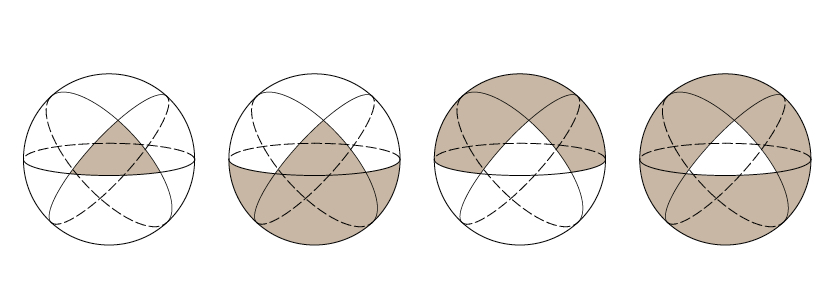
\includegraphics[width=0.9\textwidth]{kugel/Dreieckarten.jpg}
    \captionof{figure}{Dreieckarten auf einer Kugeloberfläche}
\end{center}

Der Begriff Sphärisches Dreieck oder Kugeldreieck ist ein sehr weitläufiger Begriff. 
Dabei können wir den Begriff in drei für uns wesentliche Dreiecke unterteilen:

\begin{itemize}
\item Kugelzweieck
\item Nicht Eulersche’Dreiecke
\item Eulersche’Dreiecke
\end{itemize}

\subsection{Kugelzweieck}

Zwei Grosskreise auf der Kugeloberfläche, zerlegen diese in vier gleiche Kugelzweiecke. 
Jedes dieser Dreieckseiten hat die Länge
$180^{\circ}$ oder $\pi$
Der Flächeninhalt wird dabei nur durch den Winkel $\alpha$ zwischen den beiden Grosskreisen bestimmt.

\begin{center}
        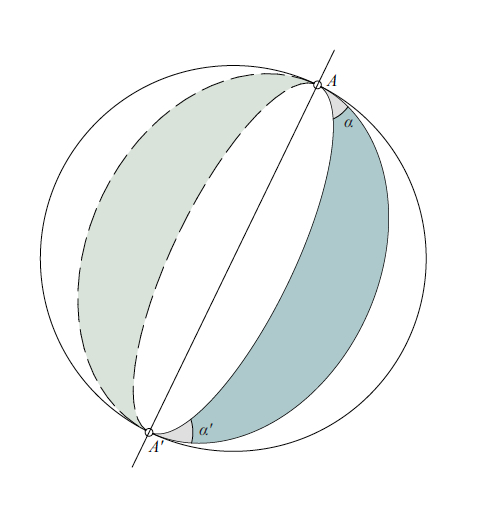
\includegraphics[width=0.3\textwidth]{kugel/Zweieck.jpg}
    \captionof{figure}{Bildung von Zweiecken durch Grosskreise}
\end{center}

Dabei ist der Flächeninhalt der ganzen Kugel:

\begin{align*}
A_{ Kugel } &= 4 \pi r^{2}
\end{align*}


Um den Flächeninhalt des betrachteten Zweieckes zu bekommen, 
müssen wir das ganze noch mit dem Kugelsegment mit dem Winkel $\alpha$ multiplizieren.

\begin{align*}
A_{ Zweieck } &= 4 \pi r^{2} \cdot \frac{ \alpha }{ 2 \pi }
\end{align*}


\subsection{Nicht Eulersche’ Dreiecke}

BLABLA

\subsection{Eulersche’ Dreiecke}

Legt man drei Grosskreise auf eine Kugeloberfläche, bilden sich dabei acht Dreiecke. 
Ein solches Dreieck heisst Eulersches’Dreieck\footnote{%
Leonard Euler (1707-1783), berühmter Schweizer Mathematiker und Physiker. 
Nicht Eulersche’Dreiecke erhält man, indem man das Äussere des Dreieckes ABC betrachtet.} 
Diese Dreiecke werden weder durch die Verlängerung ihrer Seiten durchschnitten, 
noch haben sie Dreiecksseiten welche grösser als $180^{\circ}$ sind.

\begin{center}
        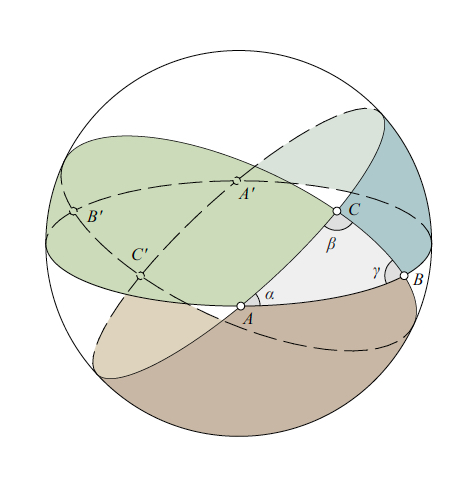
\includegraphics[width=0.4\textwidth]{kugel/Zweiecke.jpg}
    \captionof{figure}{Drei Grosskreise bilden ein sphärisches Dreieck}
\end{center}

In den nachstehenden Erklärungen und Herleitungen, sprechen wir ausschliesslich von Eulerschen’Dreiecken, da die umgeformten Winkelsätze der ebenen Trigonometrie nur auf diese Art von Kugeldreiecken angewendet werden kann.

$A_{ \overline{ ABC }}$ ist die Fläche des Dreieckes auf der Kugeloberfläche
In der ebenen Trigonometrie liegt die Winkelsumme eines Dreiecks bei
$180^{\circ}$.

Anders aber in der sphärischen Trigonometrie. Obschon sie einige Gemeinsamkeiten zur ebenen Trigonometrie aufweist, kann man nicht alles übernehmen.
So auch nicht wie Winkelsumme in einem sphärischen Dreieck.
Diese liegt bei:

\[
\begin{aligned}
\pi
&-
3\pi
&
&\text{\bigg \vert}
&
180^{\circ}
&-
540^{\circ}
\end{aligned}
\]

daraus lässt sich ableiten, das ein einzelner Winkel nicht grösser als $\pi$ oder $180^{\circ}$ sein darf. Ansonsten ist es kein Eulersches’Dreieck und wir dürfen die sphärische Trigonometrie nicht anwenden.\\
Wichtig anzumerken ist, dass die Seiten immer in Radiant beschrieben werden und nicht im Längenmass Meter wie wir es uns gewohnt sind. 
Bei den Dreiecksseiten handelt es sich um Kreisbögen und keine Strecken.

\section{Dreiecksfläche}

\begin{align*}
\text{Zweieck A}
&=
\overline{ABC} + \overline{A'BC} = 2 \alpha r^{ 2 } = A_{ \alpha }\\
\text{Zweieck B}
&=
\overline{ABC} + \overline{AB'C} = 2 \beta r^{ 2 } = A_{ \beta }\\
\text{Zweieck C}
&=
\overline{ABC} + \overline{ABC'} = 2 \gamma r^{ 2 } = A_{ \gamma }
\end{align*}

\begin{align*}
A_{ \alpha } + A_{ \beta } + A_{ \gamma } &= \frac{ 4\pi r^{ 2 } }{ 2 } + 2A_{ \overline{ ABC }} \\
2\alpha r^{ 2 } + 2\beta r^{ 2 } + 2\gamma r^{ 2 } &= \frac{ 4\pi r^{ 2 } }{ 2 } + 2A_{ \overline{ ABC }} \parallel:2\\
\alpha r^{ 2 } + \beta r^{ 2 } + \gamma r^{ 2 } &= \pi r^{ 2 } + A_{ \overline{ ABC }} \parallel-\pi r^{ 2 }\\
r^{ 2 }\left(\alpha + \beta + \gamma - \pi\right) &= A_{ \overline{ ABC }}
\end{align*}




\section{Sphärischer Exzess}
Die Winkelsumme sphärischer Dreiecke ist immer \textgreater \,  $\pi$.

\begin{align*}
\pi < \alpha + \beta + \gamma
\end{align*}

Der sphärische Exzess gibt dabei an, wie stark die Winkelsumme von $\pi$ abweicht.

\begin{align*}
\pi + \epsilon &= \alpha + \beta + \gamma \\
\epsilon &= \alpha + \beta + \gamma - \pi
\end{align*}

Würde der sphärische Exzess in der ebenen Trigonometrie angewendet, wäre dieser = 0. 
Bezieht man das auf die Erde und somit einer Kugel, kann man mit Hilfe eines beliebigen sphärischen Dreieckes und dessen Flächeninhalt auf den Radius der Kugel schliessen.

\subsection{Grenzfall - Satz von Legendre}

\begin{quote} \textit{Ein kleines sphärisches Dreieck kann näherungsweise 
wie ein ebenes Dreieck mit denselben Seiten berechnet 
werden, wenn alle Winkel des ebenen Dreiecks die um 
je ein Drittel des sphärischen Exzesses verminderten 
Winkel des sphärischen Dreiecks nimmt.} \end{quote}
\begin{flushright} - Adrien-Marie Legendre (1752-1833), Paris 1787
\end{flushright}x

Diese Aussage zeigt den Zusammenhang zwischen der 
Trigonometrie in der Ebene sowie in auf der Kugel
auf. Im speziellen bei sehr kleinen sphärischen 
Dreiecken ist die Winkelsumme nur unwesentlich 
grösser als $180^{\circ}$. Des Weiteren kann gesagt werden,
dass der sphärische Exzess gleichmässig auf alle
Winkel aufgeteilt wird.
Wichtig anzumerken ist, dass der Satz von Legendre 
für grosse, aber endliche Radien $r$ gilt.

%[SKIZZE GROSSER RADIUS/KLEINE KRÜMMUNG, KLEINER RADIUS/GROSSE KRÜMMUNG!!!!]
%


\section{Sphärisch Analoge Winkelfunktionen}

\subsection{Sphärischer Sinussatz}

Wir stellen die allgemeinen Sinussätze der Winkel $\alpha$ und $\gamma$ auf:


\[
\begin{aligned}
&{sin(\gamma)} = \frac{h}{a}
&
&\text{\bigg \vert}
&
&{sin(\alpha)} = \frac{h}{c}
&
\end{aligned}
\]

Daraus folgt:
\begin{align*}
h &= sin(\gamma)\cdot a \\
h &= sin(\alpha)\cdot c
\end{align*} 

Durch Gleichsetzung erhält man:
\begin{align*}
h &= h \\
sin(\gamma)\cdot a &= sin(\alpha)\cdot c
\end{align*} 

Durch umstellen erhalten wir den Sinussatz für a und c:
\begin{align*}
sin(\gamma)\cdot a &= sin(\alpha)\cdot c \\
\frac{sin(\gamma)}{c} &= \frac{sin(\alpha)}{a} 
\end{align*} 



\begin{align*}
\frac{sin(\alpha)}{sin(a)} = \frac{sin(\beta)}{sin(b)} = \frac{sin(\gamma)}{sin(c)}
\end{align*} 


\subsection{Winkelkosinussatz}

%[SKIZZE WINKELKOSINUS]

\[
\begin{aligned}
&\overline{C'A'} &= d\cdot {tan(b)}
&
&
&
&
&
&\overline{C'B'} &= d\cdot {tan(a)}
\end{aligned}
\]

\[
\begin{aligned}
&\overline{MA'} &= \frac{ d }{cos(b)}
&
&
&
&
&
&\overline{MB'} &= \frac{ d }{cos(a)}
\end{aligned}
\]

Der allgemeine Kosinussatz beschreibt sich wie folgt:

\begin{align*}
c^{ 2 } &= a^{ 2 } + b^{ 2 } - 2ab \cdot cos(\gamma)
\end{align*}

\begin{align*}
\triangle \overline{A'B'C' }
\overline{ A'B' }^{ 2 } &= \overline{ C'B' }^{ 2 } + \overline{ C'A' }^{ 2 } - 2 \cdot \overline{ C'B' } \cdot \overline{ C'A' } \cdot cos(\gamma)
\end{align*}



\begin{align*}
\overline{A'B'}^{ 2 } &= (d\cdot tan(a))^{ 2 } + (d\cdot tan(b))^{ 2 } - 2 \cdot (d\cdot tan(a) \cdot (d\cdot tan(b) \cdot cos(\gamma)\\
\overline{A'B'}^{ 2 } &= d^{ 2 } \cdot \left(\left(tan^{ 2 }(a) + tan^{ 2 }(b)\right) - 2\cdot tan(a) \cdot tan(b) \cdot cos(\gamma)\right)
\end{align*}

\begin{align*}
\triangle \overline{ MA'B' }
\overline{ A'B' }^{ 2 } &= \overline{ MB' }^{ 2 } + \overline{ MA' }^{ 2 } - 2\cdot \overline{ MB'} \cdot \overline{ MA' } \cdot cos(c)
\end{align*}


\begin{align*}
\overline{ A'B'}^{ 2 } &= \left(\frac{ d }{ cos(a) }  \right)^{ 2 } + \left(\frac{ d }{ cos(b)}  \right)^{ 2 } - 2 \cdot \frac{ d }{ cos(a)} \cdot \frac{ d }{ cos(b)} \cdot cos(c) \\
\overline{ A'B' }^{ 2 } &= d^{ 2 } \cdot \left(\left(\frac{ 1 }{ cos(a) }  \right)^{ 2 } + \left(\frac{ 1 }{ cos(b) }  \right)^{ 2 } - 2 \cdot \frac{ 1 }{ cos(a)} \cdot \frac{ 1 }{ cos(b)} \cdot cos(c)\right)\\
\overline{ A'B' }^{ 2 } &= d^{ 2 } \cdot \left(\left(tan^{ 2 }(a) + 1\right) + \left(tan^{ 2 }(b) + 1\right) - \left(2 \cdot \frac{cos(c)}{cos(a) \cdot cos(b)}\right)\right)
\end{align*}



\begin{align*}
\overline{ A'B'}^{ 2 } &= d^{ 2 } \cdot \left(\left(tan^{ 2 }(a) + tan^{ 2 }(b)\right) - 2 \cdot tan(a) \cdot tan(b) \cdot cos(\gamma)\right) \\
\overline{ A'B'}^{ 2 } &= d^{ 2 } \cdot \left(\left(tan^{ 2 }(a) + 1\right) + \left(tan^{ 2 }(b) + 1\right) - \left(2 \cdot \frac{cos(c)}{cos(a) \cdot cos(b)}\right)\right)
\end{align*}

Die anderen Gleichungen des Satzes, erfolgen aus Symmetriegründen.

\subsection{Seitenkosinussatz}
Durch zyklische Vertauschung des Winkelkosinus erhalten wir den Seitenkosinussatz:

\begin{align*}
{cos(a)} &= {cos(b)} \cdot {cos(c)} + {sin(b)} \cdot {sin(c)} \cdot {sin(\alpha)}\\
{cos(b)} &= {cos(a)} \cdot {cos(c)} + {sin(a)} \cdot {sin(c)} \cdot {sin(\beta)}\\
{cos(c)} &= {cos(a)} \cdot {cos(b)} + {sin(a)} \cdot {sin(b)} \cdot {sin(\gamma)}\\
\end{align*}

\section{Navigation auf See}
Das besondere an Seekarten ist die Inhaltliche Ausrichtung. Anders wie Landkarten muss sie Informationen enthalten welche für den Kapitän und seine Besatzung von grosser Bedeutung sind. Vor allem in Küstennähe ist das navigieren eines Schiffes besonders gefährlich. So enthalten Seekarten etwas über Wassertiefen, Bodenbeschaffenheiten, Gezeiten, Küstenlinien, Landzungen und Windrichtungen.
Der Hauptunterschied dabei ist, das auf der Landkarte feste Positionen definiert und aufgezeigt werden, das einzige was sich verändert ist der Reisende selbst. Bei der Seekarte ist das anders, es werden veränderliche Einwirkungen der Natur festgehalten.

Dieser kleine Unterschied zeigt die Notwendigkeit auf, die Position und den Kurs seines Schiffes auf See immer ermitteln zu können.


\section{Geographische Koordinaten}

Nachdem klar war, das die Erde eine Kugel ist, wurde diese in ein Gradnetz aufgeteilt. Dabei wurden die Angaben für eine exakte Ortsbestimmung klar definiert und die bis heute gültigen Koordinaten bestimmt.
Dabei muss man sich nochmals in Erinnerung rufen, dass sich die Erde in 24h einmal um ihre eigene Achse dreht. Nach $360 ^{\circ}$ 
und somit einer vollen Umdrehung, steht sie wieder in ihrer Ursprungsposition und ein neuer Tag beginnt.

Die Koordinaten setzen sich aus folgenden Komponenten zusammen:

\[
\begin{aligned}
&\text{Grad } (^{\circ})
&
&\text{\bigg \vert}
&
&\text{Bogenminuten } (`)
&
&\text{\bigg \vert}
&
&\text{Bogensekunden } (``)
\end{aligned}
\]

Die Erdoberfläche wurde in je 360 Breiten- und Längengrade eingeteilt. Die Breitengrade haben zueinander einen Abstand von 111.31 km, dies entspricht auch dem Abstand der Längengrade am Äquator mit Zunehmender Nähe zu den Polen, nimmt dieser Abstand ab.

\[
\begin{aligned}
&1^{\circ}
&
&\text{\bigg \vert}
&
&4 \text{ Minuten}
&
&\text{\bigg \vert}
&
&111.31\text{ km}
\end{aligned}
\]

Berechnet man nun die Erdumdrehung von 360°, erhält man genau den Erdumfang am Äquator: \begin{align*} 40’074 \text{ km.}\end{align*}

Dabei geben die Bogenminuten und -sekunden dem Standort die gewünschte Exaktheit. Mit den vollständigen Koordinaten lässt sich der Standort auf einer Landkarte exakt bestimmen und einzeichnen.

\subsection{Zeitzonen der Erde}
Wenn man nun die verschiedenen Zeitzonen der Erde betrachtet, macht die Verschiebung von jeweils einer Stunde durchaus Sinn, es lässt sich auf die Längengrade schliessen.
Zwischen den verschiedenen Zeitzonen liegen 15 Längengrade:

\begin{align*}
\text{15 Längengrade à 4 Minuten = 60 Minuten Zeitverschiebung = ca. 1665 km}
\end{align*}

Dabei ist die Zeitzone in welcher Mitte sich der Greenwich Meredian befindet die \textit{Greenwich Mean Time (GMT)} welche bis 1928 als Weltzeit galt. Im Jahr 1972 wurde diese umbenannt in die \textit{Coordinated Universal Time (UTC)} und wir von da an als Weltzeit $\pm$ 0.00 verwendet.


\section{Der Breitengrad}
Die Breitengrade bilden die bereits genannten Kleinkreise auf der Kugeloberfläche. Sie verlaufen in einem Abstand von genau 111 km parallel zum Äquator. Dabei stellt  dieser genau die Mitte zwischen Nord- und Südpol dar und teilt die Erdkugel in zwei gleiche Hälften. Somit wird von nördlicher und südlicher Breite gesprochen, je nach dem auf welcher Halbkugel man sich befindet.

%[SKIZZE DER GEOGRAFISCHEN BREITE ERDKUGEL]

\subsection{Geografische Breite $\phi$}
\begin{definition}
Die geografische Breite eines Standortes ist nichts anderes, als der Winkel am Erdmittelpunkt zwischen der Ebene des Äquators und der Geraden zum Standpunkt auf der Erdoberfläche.
\end{definition}

%[SKIZZE DER GEOGRAFISCHEN BREITE MIT WINKEL]

\subsection{Navigation mit den Breitengraden}
Da der Breitengrad bereits sehr früh ziemlich präzise bestimmt werden könnte, nutzten bereits die Seefahrer um Christoph Kolumbus den Breitengrad zur Navigation ihrer Flotten.
Den dieser lässt sich ziemlich einfach aus dem höchsten Sonnenstand oder einem Fixstern bestimmen. Dabei wird mit einem Jakobsstab\footnote{%
Der Jakobsstab ist ein früheres astronomisches Instrument zur Winkelmessung und wurde vor allem in der Seefahrt verwendet. Er ist in der Nautik der Vorläufer des Sextanten.} (später Sextant\footnote{%
Der Sextant ist ein nautisches Messinstrument zur Winkelmessung von Horizont und Fixstern (Gestirn)}) der Winkel zwischen dem Horizont und dem Fixstern gemessen. Der Winkel welchen man erhält, zieht man von 90° ab und erhält somit die geografische Breite. \\

%[SKIZZE ERMITTLUNG DES BREITENGRADES]

Wenn man sich auf der Nordhalbkugel befindet, ist der Polarstern ein sehr guter Fixstern. Befindet sich ein Schiff nun sehr nahe am Nordpol, steht dieser nahezu senkrecht am Himmelszelt bei $90^{\circ}$. Würde es aber nahe dem Äquator stehen, erscheint dieser am Horizont bei $0^{\circ}$.

\subsection{Korrekturbeiwert}

\section{Der Längengrad}
Die Längengrade bilden die bereits genannten Grosskreise auf der Kugeloberfläche.
Sie schneiden den Äquator im rechten Winkel, haben dort einen Abstand von 111 km zueinander und verbinden die Pole. Anders wie bei der geografischen Breite, ist in der Natur kein Längengrad gegeben welcher den Nullpunkt darstellt.

%[SKIZZE DER GEOGRAFISCHEN LÄNGE ERDKUGEL]

\subsection{Geografische Länge $\lambda$}
\begin{definition}
Die geografische Länge ist der Winkel an der Erdachse zum Nullmeridian.
\end{definition}

\subsection{Navigation mit den Längengraden}
Die geografische Länge lässt sich nicht so einfach bestimmen wie deren Breite. Für die Berechnung auf See benötigt man eine Referenzzeit eines Ortes mit bekannter Länge.
In der Zeit der Entdecker gab es noch keine mechanischen Uhren. Die Sonnenuhr war zudem ungeeignet, da diese nur die Uhrzeit am Standort mass und nicht die am Referenzort selbst. Die erste Pendeluhr wurde erst Mitte des 17. Jahrhunderts erfunden, was in der Schifffahrt aber auch nicht die Lösung brachte.\\
Pendeluhren auf einem Schiff sind ungeeignet, da das Pendel mit dem Wellengang aus dem Takt gebracht wird und somit die Uhr falsch geht.
Zu ungenau und gegen äussere Erschütterungen zu empfindlich waren später auch die federgetriebenen Uhren und die Unruh. Dazukamen die verschiedenen Klimazonen welche ein Schiff zu durchqueren hatten. Das Metall zog sich viel zu fest zusammen oder dehnte sich aus, was dazu führte das die Uhr unregelmässig lief.

Das sogenannte „Längenproblem“ stellte nicht nur bei der Navigation auf See ein Problem dar, es ergaben sich auch wirtschaftliche Konsequenzen. Die Schiffe mussten bis zur gewünschten geografischen Breite navigieren und segelten dann den Breitengrad entlang. Dabei waren die Schiffe oft Wochenlang unterwegs und segelten die „Breiten ab“ um an die gewünschte Position zu kommen. Dies führte zu erheblichen Zeitverlusten und viel längeren Reisezeiten.


\section{The Board of Longitude - Das Längenproblem}
Das Längenproblem beschäftigte alle grossen Seefahrernationen Europas. Wenn man bedenkt das sich Werte in einer  Höhe von halben britischen Staatshaushalten auf verloren gegangenen Schiffen befanden, erkennt man die Dringlichkeit für eine zuverlässige und genaue Navigation auf See.


\begin{itemize}
\item £ 20’000 - Abweichung von max. einem halben Grad
\item £ 15’000 - Abweichung von zwei Drittel Grad
\item £ 10’000 - Abweichung von max. $1 ^{\circ}$
\end{itemize}

\subsection{John Harrison}


\subsection{Tobias Mayer}



Uhren mit einer Abweichung von einer Minute Abweichung pro Tag (





\section{Nautische Dreieck}


$\Rightarrow$





\section{Die Vermessung der Welt}
Wir schreiben das Jahr 1818 und kehren in die Zeit des Mathematikers Carl Friedrich Gauss zurück. Neben dem liebevoll genannten „kleinen Gauss“ und anderen herausragenden Mathematischen Leistungen, beschäftigte er in den Folgejahren mit der Vermessung des Königreichs Hannovers und verfasste auf 61 Blättern das Kartenwerk \textit{Gauss’sche Landesaufnahme der 1815 durch Hannover erworbenen Gebiete}.






AUFGABE

Hubble Teleskop 
24. April 1990






\printbibliography[heading=subbibliography]
\end{refsection}




%\chapter{Geometrie auf der Kugeloberfläche\label{chapter:kugel}}
\lhead{Geometrie auf der Kugeloberfläche}
\begin{refsection}
\chapterauthor{Melina Staub und Fabian Schmid}

\section{Einleitung}

Schon seit jeher fasziniert den Menschen die Fahrt zur See. Nicht grundlos ist die Seefahrt eine der wichtigsten und ältesten Tätigkeiten der Menschheit. Der innerliche Drang neue Weltmeere und unbekannte Gebiete zu entdecken, die Fahrt zur See zu erleichtern und erträglicher zu machen, trieben die Menschen an, die Schiffe dieser Welt immer weiter zu entwickeln.

Die Idee der Kugelform der Erde ist älter als man zu denken vermag. Bereits der Schüler des antiken griechischen Philosophen Platon - Aristoteles schrieb in seiner Schrift \textit{Über den Himmel} aus dem 4. Jahrhundert v. Chr. etliche Gründe welche für die Gestallt der Erde als Kugel sprechen:

\begin{itemize}
      \item Sämtliche schweren Körper streben zum Mittelpunkt des Alls. Da sie dies von allen Seiten her gleichmäßig tun und die Erde im Mittelpunkt des Alls steht, muss sie eine kugelrunde Gestalt annehmen. 
\item Bei von der Küste wegfahrende Schiffen wird der Rumpf vor den Segeln der Sicht verborgen. 
\item In südlichen Ländern erscheinen südliche Sternbilder höher über dem Horizont.
\item Der Erdschatten bei einer Mondfinsternis ist stets rund.
\end{itemize}

Jedoch war um 1492 - der Zeit der Entdeckung Amerikas durch Christoph Kolumbus, die Idee der Erde in Kugelform noch sehr umstritten. Er erkannte anhand den Theorien und Erkenntnissen der alten Griechen, vor allem Aristoteles, das die Erde eine Kugel sein muss. \\
Doch mit seinem Vorschlag einen Seeweg über den Atlantik nach Indien zu finden und nicht wie üblich um Afrika zu segeln, stiess er beim beim portugiesischen König auf taube Ohren. Sein Plan Indien über eine Route nach Westen zu erreichen, widersprach dem gesunden Menschenverstand. Wäre die Erde wirklich eine Kugel und man befände sich auf der unteren Erdhalbkugel, würde man herunterfallen.\\
Doch auch der damals übliche Glaube an die Erde in Scheibenform brachte so einige Risiken mit sich. Was würde passieren, wenn die Flotte das Ende der Scheibe erreicht hatte? Würden sie über den Erdrand hinweggleiten und in den Abgrund stürzen?\\
Erst nach viel Überzeugungsarbeit durch Kolumbus, setzte er sich am Spanischen Hof durch und segelte über die Westliche Route über den Atlantik und entdeckte schlussendlich Amerika.

Der praktische und greifbare Beweis das die Erde eine Kugel ist, lieferte rund 30 Jahre später der Portugiese Fernando Magellan. Mit seiner Weltumsegelung und seiner Ankunft in den Philippinen, bewies er definitiv das die Erde eine Kugel ist.\\

Nun wollen wir uns die Frage stellen, wie die alten Seefahrer ohne GPS und jeglichen modernen Navigationssystemen auf hoher See wussten wo sie sich befinden und was haben die Sterne mit alldem zu tun? Reisen Sie mit uns zurück in eine Zeit mit Sextant, Kompass und Sternkarten. In die Zeit der Seefahrer und Entdecker.


\section{Geometrie auf der Ebene und der Kugel}

Euklid von Alexandria beschrieb die Grundbegriffe der ebenen Geometrie mittels Punkt, Geraden, Ebene, Winkel und Dreieck. Diese Dreiecke lassen sich mithilfe der ebenen Trigonometrie beschreiben. Dabei gelten die uns bekannten trigonometrischen Winkelfunktionen:\\

\text{Sinussatz:}
\begin{align*}
\frac{ a }{ sin(\alpha) } &= \frac{ b }{sin(\beta)} = \frac{ c }{ sin(\gamma) } = \frac{abc}{2A} = 2r\\
\end{align*}

\text{Cosinussatz:}
\begin{align*}
c^{ 2 } &= a^{ 2 } + b^{ 2 } - 2ab\cdot cos(\gamma)\\
b^{ 2 } &= a^{ 2 } + c^{ 2 } - 2ab\cdot cos(\beta)\\
a^{ 2 } &= b^{ 2 } + c^{ 2 } - 2ab\cdot cos(\alpha)
\end{align*}

Um Dreiecke auf der Kugeloberfläche zu berechnen, benötigt man die sphärische Trigonometrie. Die oben beschriebenen Sätze lassen sich auf der Kugel nicht anwenden, sie werden aber als Grundlage zur Herleitung der Sätze für das Kugeldreieck benötigt.

Die nachfolgenden Seiten thematisieren die Geometrie auf der Kugeloberfläche und wie sie in der Navigation eingesetzt werden kann.


\section{Gross- und Kleinkreise}

Eine Kugeloberfläche lässt sich in zwei verschiedene Kreisarten einteilen -  Gross- und Kleinkreise. 
Wir betrachten als erstes die Grosskreise:

\begin{definition}
Ein Großkreis ist ein größtmöglicher Kreis auf einer Kugeloberfläche. Sein Mittelpunkt fällt immer mit dem Mittelpunkt der Kugel zusammen und ein Schnitt auf dem Großkreis teilt die Kugel in jedem Fall in zwei („gleich große“) Hälften.
\end{definition}

Es gibt unendlich viele Möglichkeiten, eine Kugel in zwei gleich grosse Stücke zu zerschneiden, 
daher gibt es auch unendlich viele Grosskreise. Wenn wir die Grosskreise auf einer Kugel mit diesen auf der Erde beschreiben, sprechen wir von den Längengraden aber auch der Äquator beschreibt einen Grosskreis.
Ein Elementarer Bestandteil bilden die Grosskreise in der sphärischen Trigonometrie. Mithilfe der Schnittpunkte verschiedener Grosskreise, lässt sich ein Sphärisches Dreieck bilden auf welchem sich die sphärische Trigonometrie anwenden lässt.

[GRAFIK GROSSKREISE]

\begin{definition}
Unter Kleinkreis versteht man jene Kreise auf einer Kugeloberfläche, deren Ebenen nicht den Kugelmittelpunkt enthalten.
\end{definition}

Die Kleinkreise eignen sich im Gegensatz zu den Grosskreisen \textit{nicht} für die sphärische Trigonometrie. 
Sie werden lediglich zur Bestimmung der Messgrössen, Winkelabstände oder des Höhenwinkels eines Gestirns verwendet. 

Wenn wir die Kleinkreise auf die Erdoberfläche projizieren betrachten wir die Breitengrade.

[GRAFIK KLEINKREISE]


\section{Sphärische Dreiecke / Kugeldreieck}

\begin{center}
        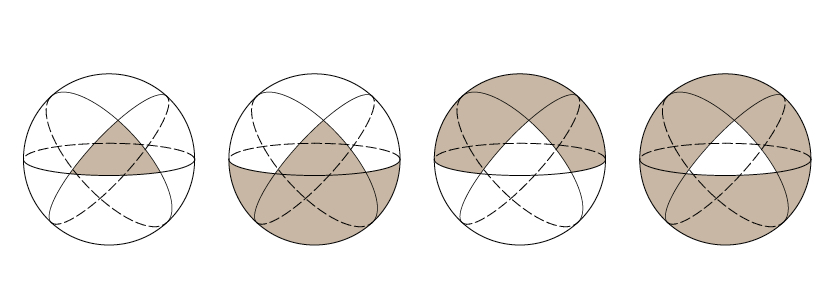
\includegraphics[width=0.9\textwidth]{kugel/Dreieckarten.jpg}
    \captionof{figure}{Dreieckarten auf einer Kugeloberfläche}
\end{center}

Der Begriff Sphärisches Dreieck oder Kugeldreieck ist ein sehr weitläufiger Begriff. 
Dabei können wir den Begriff in drei für uns wesentliche Dreiecke unterteilen:

\begin{itemize}
\item Kugelzweieck
\item Nicht Eulersche’Dreiecke
\item Eulersche’Dreiecke
\end{itemize}

\subsection{Kugelzweieck}

Zwei Grosskreise auf der Kugeloberfläche, zerlegen diese in vier gleiche Kugelzweiecke. 
Jedes dieser Dreieckseiten hat die Länge
$180^{\circ}$ oder $\pi$
Der Flächeninhalt wird dabei nur durch den Winkel $\alpha$ zwischen den beiden Grosskreisen bestimmt.

\begin{center}
        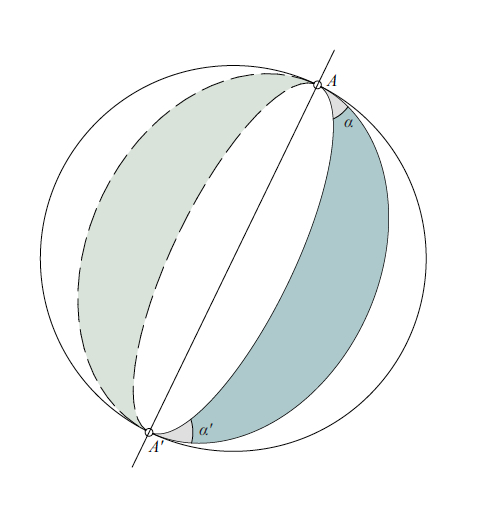
\includegraphics[width=0.3\textwidth]{kugel/Zweieck.jpg}
    \captionof{figure}{Bildung von Zweiecken durch Grosskreise}
\end{center}

Dabei ist der Flächeninhalt der ganzen Kugel:

\begin{align*}
A_{ Kugel } &= 4 \pi r^{2}
\end{align*}


Um den Flächeninhalt des betrachteten Zweieckes zu bekommen, 
müssen wir das ganze noch mit dem Kugelsegment mit dem Winkel $\alpha$ multiplizieren.

\begin{align*}
A_{ Zweieck } &= 4 \pi r^{2} \cdot \frac{ \alpha }{ 2 \pi }
\end{align*}


\subsection{Nicht Eulersche’ Dreiecke}

BLABLA

\subsection{Eulersche’ Dreiecke}

Legt man drei Grosskreise auf eine Kugeloberfläche, bilden sich dabei acht Dreiecke. 
Ein solches Dreieck heisst Eulersches’Dreieck\footnote{%
Leonard Euler (1707-1783), berühmter Schweizer Mathematiker und Physiker. 
Nicht Eulersche’Dreiecke erhält man, indem man das Äussere des Dreieckes ABC betrachtet.} 
Diese Dreiecke werden weder durch die Verlängerung ihrer Seiten durchschnitten, 
noch haben sie Dreiecksseiten welche grösser als $180^{\circ}$ sind.

\begin{center}
        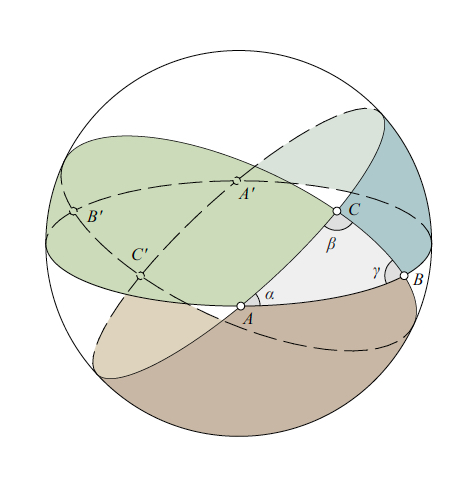
\includegraphics[width=0.4\textwidth]{kugel/Zweiecke.jpg}
    \captionof{figure}{Drei Grosskreise bilden ein sphärisches Dreieck}
\end{center}

In den nachstehenden Erklärungen und Herleitungen, sprechen wir ausschliesslich von Eulerschen’Dreiecken, da die umgeformten Winkelsätze der ebenen Trigonometrie nur auf diese Art von Kugeldreiecken angewendet werden kann.

$A_{ \overline{ ABC }}$ ist die Fläche des Dreieckes auf der Kugeloberfläche
In der ebenen Trigonometrie liegt die Winkelsumme eines Dreiecks bei
$180^{\circ}$.

Anders aber in der sphärischen Trigonometrie. Obschon sie einige Gemeinsamkeiten zur ebenen Trigonometrie aufweist, kann man nicht alles übernehmen.
So auch nicht wie Winkelsumme in einem sphärischen Dreieck.
Diese liegt bei:

\[
\begin{aligned}
\pi
&-
3\pi
&
&\text{\bigg \vert}
&
180^{\circ}
&-
540^{\circ}
\end{aligned}
\]

daraus lässt sich ableiten, das ein einzelner Winkel nicht grösser als $\pi$ oder $180^{\circ}$ sein darf. Ansonsten ist es kein Eulersches’Dreieck und wir dürfen die sphärische Trigonometrie nicht anwenden.\\
Wichtig anzumerken ist, dass die Seiten immer in Radiant beschrieben werden und nicht im Längenmass Meter wie wir es uns gewohnt sind. 
Bei den Dreiecksseiten handelt es sich um Kreisbögen und keine Strecken.

\section{Dreiecksfläche}

\begin{align*}
\text{Zweieck A}
&=
\overline{ABC} + \overline{A'BC} = 2 \alpha r^{ 2 } = A_{ \alpha }\\
\text{Zweieck B}
&=
\overline{ABC} + \overline{AB'C} = 2 \beta r^{ 2 } = A_{ \beta }\\
\text{Zweieck C}
&=
\overline{ABC} + \overline{ABC'} = 2 \gamma r^{ 2 } = A_{ \gamma }
\end{align*}

\begin{align*}
A_{ \alpha } + A_{ \beta } + A_{ \gamma } &= \frac{ 4\pi r^{ 2 } }{ 2 } + 2A_{ \overline{ ABC }} \\
2\alpha r^{ 2 } + 2\beta r^{ 2 } + 2\gamma r^{ 2 } &= \frac{ 4\pi r^{ 2 } }{ 2 } + 2A_{ \overline{ ABC }} \parallel:2\\
\alpha r^{ 2 } + \beta r^{ 2 } + \gamma r^{ 2 } &= \pi r^{ 2 } + A_{ \overline{ ABC }} \parallel-\pi r^{ 2 }\\
r^{ 2 }\left(\alpha + \beta + \gamma - \pi\right) &= A_{ \overline{ ABC }}
\end{align*}




\section{Sphärischer Exzess}
Die Winkelsumme sphärischer Dreiecke ist immer \textgreater \,  $\pi$.

\begin{align*}
\pi < \alpha + \beta + \gamma
\end{align*}

Der sphärische Exzess gibt dabei an, wie stark die Winkelsumme von $\pi$ abweicht.

\begin{align*}
\pi + \epsilon &= \alpha + \beta + \gamma \\
\epsilon &= \alpha + \beta + \gamma - \pi
\end{align*}

Würde der sphärische Exzess in der ebenen Trigonometrie angewendet, wäre dieser = 0. 
Bezieht man das auf die Erde und somit einer Kugel, kann man mit Hilfe eines beliebigen sphärischen Dreieckes und dessen Flächeninhalt auf den Radius der Kugel schliessen.

\subsection{Grenzfall - Satz von Legendre}

\begin{quote} \textit{Ein kleines sphärisches Dreieck kann näherungsweise 
wie ein ebenes Dreieck mit denselben Seiten berechnet 
werden, wenn alle Winkel des ebenen Dreiecks die um 
je ein Drittel des sphärischen Exzesses verminderten 
Winkel des sphärischen Dreiecks nimmt.} \end{quote}
\begin{flushright} - Adrien-Marie Legendre (1752-1833), Paris 1787
\end{flushright}x

Diese Aussage zeigt den Zusammenhang zwischen der 
Trigonometrie in der Ebene sowie in auf der Kugel
auf. Im speziellen bei sehr kleinen sphärischen 
Dreiecken ist die Winkelsumme nur unwesentlich 
grösser als $180^{\circ}$. Des Weiteren kann gesagt werden,
dass der sphärische Exzess gleichmässig auf alle
Winkel aufgeteilt wird.
Wichtig anzumerken ist, dass der Satz von Legendre 
für grosse, aber endliche Radien $r$ gilt.

%[SKIZZE GROSSER RADIUS/KLEINE KRÜMMUNG, KLEINER RADIUS/GROSSE KRÜMMUNG!!!!]
%


\section{Sphärisch Analoge Winkelfunktionen}

\subsection{Sphärischer Sinussatz}

Wir stellen die allgemeinen Sinussätze der Winkel $\alpha$ und $\gamma$ auf:


\[
\begin{aligned}
&{sin(\gamma)} = \frac{h}{a}
&
&\text{\bigg \vert}
&
&{sin(\alpha)} = \frac{h}{c}
&
\end{aligned}
\]

Daraus folgt:
\begin{align*}
h &= sin(\gamma)\cdot a \\
h &= sin(\alpha)\cdot c
\end{align*} 

Durch Gleichsetzung erhält man:
\begin{align*}
h &= h \\
sin(\gamma)\cdot a &= sin(\alpha)\cdot c
\end{align*} 

Durch umstellen erhalten wir den Sinussatz für a und c:
\begin{align*}
sin(\gamma)\cdot a &= sin(\alpha)\cdot c \\
\frac{sin(\gamma)}{c} &= \frac{sin(\alpha)}{a} 
\end{align*} 



\begin{align*}
\frac{sin(\alpha)}{sin(a)} = \frac{sin(\beta)}{sin(b)} = \frac{sin(\gamma)}{sin(c)}
\end{align*} 


\subsection{Winkelkosinussatz}

%[SKIZZE WINKELKOSINUS]

\[
\begin{aligned}
&\overline{C'A'} &= d\cdot {tan(b)}
&
&
&
&
&
&\overline{C'B'} &= d\cdot {tan(a)}
\end{aligned}
\]

\[
\begin{aligned}
&\overline{MA'} &= \frac{ d }{cos(b)}
&
&
&
&
&
&\overline{MB'} &= \frac{ d }{cos(a)}
\end{aligned}
\]

Der allgemeine Kosinussatz beschreibt sich wie folgt:

\begin{align*}
c^{ 2 } &= a^{ 2 } + b^{ 2 } - 2ab \cdot cos(\gamma)
\end{align*}

\begin{align*}
\triangle \overline{A'B'C' }
\overline{ A'B' }^{ 2 } &= \overline{ C'B' }^{ 2 } + \overline{ C'A' }^{ 2 } - 2 \cdot \overline{ C'B' } \cdot \overline{ C'A' } \cdot cos(\gamma)
\end{align*}



\begin{align*}
\overline{A'B'}^{ 2 } &= (d\cdot tan(a))^{ 2 } + (d\cdot tan(b))^{ 2 } - 2 \cdot (d\cdot tan(a) \cdot (d\cdot tan(b) \cdot cos(\gamma)\\
\overline{A'B'}^{ 2 } &= d^{ 2 } \cdot \left(\left(tan^{ 2 }(a) + tan^{ 2 }(b)\right) - 2\cdot tan(a) \cdot tan(b) \cdot cos(\gamma)\right)
\end{align*}

\begin{align*}
\triangle \overline{ MA'B' }
\overline{ A'B' }^{ 2 } &= \overline{ MB' }^{ 2 } + \overline{ MA' }^{ 2 } - 2\cdot \overline{ MB'} \cdot \overline{ MA' } \cdot cos(c)
\end{align*}


\begin{align*}
\overline{ A'B'}^{ 2 } &= \left(\frac{ d }{ cos(a) }  \right)^{ 2 } + \left(\frac{ d }{ cos(b)}  \right)^{ 2 } - 2 \cdot \frac{ d }{ cos(a)} \cdot \frac{ d }{ cos(b)} \cdot cos(c) \\
\overline{ A'B' }^{ 2 } &= d^{ 2 } \cdot \left(\left(\frac{ 1 }{ cos(a) }  \right)^{ 2 } + \left(\frac{ 1 }{ cos(b) }  \right)^{ 2 } - 2 \cdot \frac{ 1 }{ cos(a)} \cdot \frac{ 1 }{ cos(b)} \cdot cos(c)\right)\\
\overline{ A'B' }^{ 2 } &= d^{ 2 } \cdot \left(\left(tan^{ 2 }(a) + 1\right) + \left(tan^{ 2 }(b) + 1\right) - \left(2 \cdot \frac{cos(c)}{cos(a) \cdot cos(b)}\right)\right)
\end{align*}



\begin{align*}
\overline{ A'B'}^{ 2 } &= d^{ 2 } \cdot \left(\left(tan^{ 2 }(a) + tan^{ 2 }(b)\right) - 2 \cdot tan(a) \cdot tan(b) \cdot cos(\gamma)\right) \\
\overline{ A'B'}^{ 2 } &= d^{ 2 } \cdot \left(\left(tan^{ 2 }(a) + 1\right) + \left(tan^{ 2 }(b) + 1\right) - \left(2 \cdot \frac{cos(c)}{cos(a) \cdot cos(b)}\right)\right)
\end{align*}

Die anderen Gleichungen des Satzes, erfolgen aus Symmetriegründen.

\subsection{Seitenkosinussatz}
Durch zyklische Vertauschung des Winkelkosinus erhalten wir den Seitenkosinussatz:

\begin{align*}
{cos(a)} &= {cos(b)} \cdot {cos(c)} + {sin(b)} \cdot {sin(c)} \cdot {sin(\alpha)}\\
{cos(b)} &= {cos(a)} \cdot {cos(c)} + {sin(a)} \cdot {sin(c)} \cdot {sin(\beta)}\\
{cos(c)} &= {cos(a)} \cdot {cos(b)} + {sin(a)} \cdot {sin(b)} \cdot {sin(\gamma)}\\
\end{align*}

\section{Navigation auf See}
Das besondere an Seekarten ist die Inhaltliche Ausrichtung. Anders wie Landkarten muss sie Informationen enthalten welche für den Kapitän und seine Besatzung von grosser Bedeutung sind. Vor allem in Küstennähe ist das navigieren eines Schiffes besonders gefährlich. So enthalten Seekarten etwas über Wassertiefen, Bodenbeschaffenheiten, Gezeiten, Küstenlinien, Landzungen und Windrichtungen.
Der Hauptunterschied dabei ist, das auf der Landkarte feste Positionen definiert und aufgezeigt werden, das einzige was sich verändert ist der Reisende selbst. Bei der Seekarte ist das anders, es werden veränderliche Einwirkungen der Natur festgehalten.

Dieser kleine Unterschied zeigt die Notwendigkeit auf, die Position und den Kurs seines Schiffes auf See immer ermitteln zu können.


\section{Geographische Koordinaten}

Nachdem klar war, das die Erde eine Kugel ist, wurde diese in ein Gradnetz aufgeteilt. Dabei wurden die Angaben für eine exakte Ortsbestimmung klar definiert und die bis heute gültigen Koordinaten bestimmt.
Dabei muss man sich nochmals in Erinnerung rufen, dass sich die Erde in 24h einmal um ihre eigene Achse dreht. Nach $360 ^{\circ}$ 
und somit einer vollen Umdrehung, steht sie wieder in ihrer Ursprungsposition und ein neuer Tag beginnt.

Die Koordinaten setzen sich aus folgenden Komponenten zusammen:

\[
\begin{aligned}
&\text{Grad } (^{\circ})
&
&\text{\bigg \vert}
&
&\text{Bogenminuten } (`)
&
&\text{\bigg \vert}
&
&\text{Bogensekunden } (``)
\end{aligned}
\]

Die Erdoberfläche wurde in je 360 Breiten- und Längengrade eingeteilt. Die Breitengrade haben zueinander einen Abstand von 111.31 km, dies entspricht auch dem Abstand der Längengrade am Äquator mit Zunehmender Nähe zu den Polen, nimmt dieser Abstand ab.

\[
\begin{aligned}
&1^{\circ}
&
&\text{\bigg \vert}
&
&4 \text{ Minuten}
&
&\text{\bigg \vert}
&
&111.31\text{ km}
\end{aligned}
\]

Berechnet man nun die Erdumdrehung von 360°, erhält man genau den Erdumfang am Äquator: \begin{align*} 40’074 \text{ km.}\end{align*}

Dabei geben die Bogenminuten und -sekunden dem Standort die gewünschte Exaktheit. Mit den vollständigen Koordinaten lässt sich der Standort auf einer Landkarte exakt bestimmen und einzeichnen.

\subsection{Zeitzonen der Erde}
Wenn man nun die verschiedenen Zeitzonen der Erde betrachtet, macht die Verschiebung von jeweils einer Stunde durchaus Sinn, es lässt sich auf die Längengrade schliessen.
Zwischen den verschiedenen Zeitzonen liegen 15 Längengrade:

\begin{align*}
\text{15 Längengrade à 4 Minuten = 60 Minuten Zeitverschiebung = ca. 1665 km}
\end{align*}

Dabei ist die Zeitzone in welcher Mitte sich der Greenwich Meredian befindet die \textit{Greenwich Mean Time (GMT)} welche bis 1928 als Weltzeit galt. Im Jahr 1972 wurde diese umbenannt in die \textit{Coordinated Universal Time (UTC)} und wir von da an als Weltzeit $\pm$ 0.00 verwendet.


\section{Der Breitengrad}
Die Breitengrade bilden die bereits genannten Kleinkreise auf der Kugeloberfläche. Sie verlaufen in einem Abstand von genau 111 km parallel zum Äquator. Dabei stellt  dieser genau die Mitte zwischen Nord- und Südpol dar und teilt die Erdkugel in zwei gleiche Hälften. Somit wird von nördlicher und südlicher Breite gesprochen, je nach dem auf welcher Halbkugel man sich befindet.

%[SKIZZE DER GEOGRAFISCHEN BREITE ERDKUGEL]

\subsection{Geografische Breite $\phi$}
\begin{definition}
Die geografische Breite eines Standortes ist nichts anderes, als der Winkel am Erdmittelpunkt zwischen der Ebene des Äquators und der Geraden zum Standpunkt auf der Erdoberfläche.
\end{definition}

%[SKIZZE DER GEOGRAFISCHEN BREITE MIT WINKEL]

\subsection{Navigation mit den Breitengraden}
Da der Breitengrad bereits sehr früh ziemlich präzise bestimmt werden könnte, nutzten bereits die Seefahrer um Christoph Kolumbus den Breitengrad zur Navigation ihrer Flotten.
Den dieser lässt sich ziemlich einfach aus dem höchsten Sonnenstand oder einem Fixstern bestimmen. Dabei wird mit einem Jakobsstab\footnote{%
Der Jakobsstab ist ein früheres astronomisches Instrument zur Winkelmessung und wurde vor allem in der Seefahrt verwendet. Er ist in der Nautik der Vorläufer des Sextanten.} (später Sextant\footnote{%
Der Sextant ist ein nautisches Messinstrument zur Winkelmessung von Horizont und Fixstern (Gestirn)}) der Winkel zwischen dem Horizont und dem Fixstern gemessen. Der Winkel welchen man erhält, zieht man von 90° ab und erhält somit die geografische Breite. \\

%[SKIZZE ERMITTLUNG DES BREITENGRADES]

Wenn man sich auf der Nordhalbkugel befindet, ist der Polarstern ein sehr guter Fixstern. Befindet sich ein Schiff nun sehr nahe am Nordpol, steht dieser nahezu senkrecht am Himmelszelt bei $90^{\circ}$. Würde es aber nahe dem Äquator stehen, erscheint dieser am Horizont bei $0^{\circ}$.

\subsection{Korrekturbeiwert}

\section{Der Längengrad}
Die Längengrade bilden die bereits genannten Grosskreise auf der Kugeloberfläche.
Sie schneiden den Äquator im rechten Winkel, haben dort einen Abstand von 111 km zueinander und verbinden die Pole. Anders wie bei der geografischen Breite, ist in der Natur kein Längengrad gegeben welcher den Nullpunkt darstellt.

%[SKIZZE DER GEOGRAFISCHEN LÄNGE ERDKUGEL]

\subsection{Geografische Länge $\lambda$}
\begin{definition}
Die geografische Länge ist der Winkel an der Erdachse zum Nullmeridian.
\end{definition}

\subsection{Navigation mit den Längengraden}
Die geografische Länge lässt sich nicht so einfach bestimmen wie deren Breite. Für die Berechnung auf See benötigt man eine Referenzzeit eines Ortes mit bekannter Länge.
In der Zeit der Entdecker gab es noch keine mechanischen Uhren. Die Sonnenuhr war zudem ungeeignet, da diese nur die Uhrzeit am Standort mass und nicht die am Referenzort selbst. Die erste Pendeluhr wurde erst Mitte des 17. Jahrhunderts erfunden, was in der Schifffahrt aber auch nicht die Lösung brachte.\\
Pendeluhren auf einem Schiff sind ungeeignet, da das Pendel mit dem Wellengang aus dem Takt gebracht wird und somit die Uhr falsch geht.
Zu ungenau und gegen äussere Erschütterungen zu empfindlich waren später auch die federgetriebenen Uhren und die Unruh. Dazukamen die verschiedenen Klimazonen welche ein Schiff zu durchqueren hatten. Das Metall zog sich viel zu fest zusammen oder dehnte sich aus, was dazu führte das die Uhr unregelmässig lief.

Das sogenannte „Längenproblem“ stellte nicht nur bei der Navigation auf See ein Problem dar, es ergaben sich auch wirtschaftliche Konsequenzen. Die Schiffe mussten bis zur gewünschten geografischen Breite navigieren und segelten dann den Breitengrad entlang. Dabei waren die Schiffe oft Wochenlang unterwegs und segelten die „Breiten ab“ um an die gewünschte Position zu kommen. Dies führte zu erheblichen Zeitverlusten und viel längeren Reisezeiten.


\section{The Board of Longitude - Das Längenproblem}
Das Längenproblem beschäftigte alle grossen Seefahrernationen Europas. Wenn man bedenkt das sich Werte in einer  Höhe von halben britischen Staatshaushalten auf verloren gegangenen Schiffen befanden, erkennt man die Dringlichkeit für eine zuverlässige und genaue Navigation auf See.


\begin{itemize}
\item £ 20’000 - Abweichung von max. einem halben Grad
\item £ 15’000 - Abweichung von zwei Drittel Grad
\item £ 10’000 - Abweichung von max. $1 ^{\circ}$
\end{itemize}

\subsection{John Harrison}


\subsection{Tobias Mayer}



Uhren mit einer Abweichung von einer Minute Abweichung pro Tag (





\section{Nautische Dreieck}


$\Rightarrow$





\section{Die Vermessung der Welt}
Wir schreiben das Jahr 1818 und kehren in die Zeit des Mathematikers Carl Friedrich Gauss zurück. Neben dem liebevoll genannten „kleinen Gauss“ und anderen herausragenden Mathematischen Leistungen, beschäftigte er in den Folgejahren mit der Vermessung des Königreichs Hannovers und verfasste auf 61 Blättern das Kartenwerk \textit{Gauss’sche Landesaufnahme der 1815 durch Hannover erworbenen Gebiete}.






AUFGABE

Hubble Teleskop 
24. April 1990






\printbibliography[heading=subbibliography]
\end{refsection}




%\chapter{Geometrie auf der Kugeloberfläche\label{chapter:kugel}}
\lhead{Geometrie auf der Kugeloberfläche}
\begin{refsection}
\chapterauthor{Melina Staub und Fabian Schmid}

\section{Einleitung}

Schon seit jeher fasziniert den Menschen die Fahrt zur See. Nicht grundlos ist die Seefahrt eine der wichtigsten und ältesten Tätigkeiten der Menschheit. Der innerliche Drang neue Weltmeere und unbekannte Gebiete zu entdecken, die Fahrt zur See zu erleichtern und erträglicher zu machen, trieben die Menschen an, die Schiffe dieser Welt immer weiter zu entwickeln.

Die Idee der Kugelform der Erde ist älter als man zu denken vermag. Bereits der Schüler des antiken griechischen Philosophen Platon - Aristoteles schrieb in seiner Schrift \textit{Über den Himmel} aus dem 4. Jahrhundert v. Chr. etliche Gründe welche für die Gestallt der Erde als Kugel sprechen:

\begin{itemize}
      \item Sämtliche schweren Körper streben zum Mittelpunkt des Alls. Da sie dies von allen Seiten her gleichmäßig tun und die Erde im Mittelpunkt des Alls steht, muss sie eine kugelrunde Gestalt annehmen. 
\item Bei von der Küste wegfahrende Schiffen wird der Rumpf vor den Segeln der Sicht verborgen. 
\item In südlichen Ländern erscheinen südliche Sternbilder höher über dem Horizont.
\item Der Erdschatten bei einer Mondfinsternis ist stets rund.
\end{itemize}

Jedoch war um 1492 - der Zeit der Entdeckung Amerikas durch Christoph Kolumbus, die Idee der Erde in Kugelform noch sehr umstritten. Er erkannte anhand den Theorien und Erkenntnissen der alten Griechen, vor allem Aristoteles, das die Erde eine Kugel sein muss. \\
Doch mit seinem Vorschlag einen Seeweg über den Atlantik nach Indien zu finden und nicht wie üblich um Afrika zu segeln, stiess er beim beim portugiesischen König auf taube Ohren. Sein Plan Indien über eine Route nach Westen zu erreichen, widersprach dem gesunden Menschenverstand. Wäre die Erde wirklich eine Kugel und man befände sich auf der unteren Erdhalbkugel, würde man herunterfallen.\\
Doch auch der damals übliche Glaube an die Erde in Scheibenform brachte so einige Risiken mit sich. Was würde passieren, wenn die Flotte das Ende der Scheibe erreicht hatte? Würden sie über den Erdrand hinweggleiten und in den Abgrund stürzen?\\
Erst nach viel Überzeugungsarbeit durch Kolumbus, setzte er sich am Spanischen Hof durch und segelte über die Westliche Route über den Atlantik und entdeckte schlussendlich Amerika.

Der praktische und greifbare Beweis das die Erde eine Kugel ist, lieferte rund 30 Jahre später der Portugiese Fernando Magellan. Mit seiner Weltumsegelung und seiner Ankunft in den Philippinen, bewies er definitiv das die Erde eine Kugel ist.\\

Nun wollen wir uns die Frage stellen, wie die alten Seefahrer ohne GPS und jeglichen modernen Navigationssystemen auf hoher See wussten wo sie sich befinden und was haben die Sterne mit alldem zu tun? Reisen Sie mit uns zurück in eine Zeit mit Sextant, Kompass und Sternkarten. In die Zeit der Seefahrer und Entdecker.


\section{Geometrie auf der Ebene und der Kugel}

Euklid von Alexandria beschrieb die Grundbegriffe der ebenen Geometrie mittels Punkt, Geraden, Ebene, Winkel und Dreieck. Diese Dreiecke lassen sich mithilfe der ebenen Trigonometrie beschreiben. Dabei gelten die uns bekannten trigonometrischen Winkelfunktionen:\\

\text{Sinussatz:}
\begin{align*}
\frac{ a }{ sin(\alpha) } &= \frac{ b }{sin(\beta)} = \frac{ c }{ sin(\gamma) } = \frac{abc}{2A} = 2r\\
\end{align*}

\text{Cosinussatz:}
\begin{align*}
c^{ 2 } &= a^{ 2 } + b^{ 2 } - 2ab\cdot cos(\gamma)\\
b^{ 2 } &= a^{ 2 } + c^{ 2 } - 2ab\cdot cos(\beta)\\
a^{ 2 } &= b^{ 2 } + c^{ 2 } - 2ab\cdot cos(\alpha)
\end{align*}

Um Dreiecke auf der Kugeloberfläche zu berechnen, benötigt man die sphärische Trigonometrie. Die oben beschriebenen Sätze lassen sich auf der Kugel nicht anwenden, sie werden aber als Grundlage zur Herleitung der Sätze für das Kugeldreieck benötigt.

Die nachfolgenden Seiten thematisieren die Geometrie auf der Kugeloberfläche und wie sie in der Navigation eingesetzt werden kann.


\section{Gross- und Kleinkreise}

Eine Kugeloberfläche lässt sich in zwei verschiedene Kreisarten einteilen -  Gross- und Kleinkreise. 
Wir betrachten als erstes die Grosskreise:

\begin{definition}
Ein Großkreis ist ein größtmöglicher Kreis auf einer Kugeloberfläche. Sein Mittelpunkt fällt immer mit dem Mittelpunkt der Kugel zusammen und ein Schnitt auf dem Großkreis teilt die Kugel in jedem Fall in zwei („gleich große“) Hälften.
\end{definition}

Es gibt unendlich viele Möglichkeiten, eine Kugel in zwei gleich grosse Stücke zu zerschneiden, 
daher gibt es auch unendlich viele Grosskreise. Wenn wir die Grosskreise auf einer Kugel mit diesen auf der Erde beschreiben, sprechen wir von den Längengraden aber auch der Äquator beschreibt einen Grosskreis.
Ein Elementarer Bestandteil bilden die Grosskreise in der sphärischen Trigonometrie. Mithilfe der Schnittpunkte verschiedener Grosskreise, lässt sich ein Sphärisches Dreieck bilden auf welchem sich die sphärische Trigonometrie anwenden lässt.

[GRAFIK GROSSKREISE]

\begin{definition}
Unter Kleinkreis versteht man jene Kreise auf einer Kugeloberfläche, deren Ebenen nicht den Kugelmittelpunkt enthalten.
\end{definition}

Die Kleinkreise eignen sich im Gegensatz zu den Grosskreisen \textit{nicht} für die sphärische Trigonometrie. 
Sie werden lediglich zur Bestimmung der Messgrössen, Winkelabstände oder des Höhenwinkels eines Gestirns verwendet. 

Wenn wir die Kleinkreise auf die Erdoberfläche projizieren betrachten wir die Breitengrade.

[GRAFIK KLEINKREISE]


\section{Sphärische Dreiecke / Kugeldreieck}

\begin{center}
        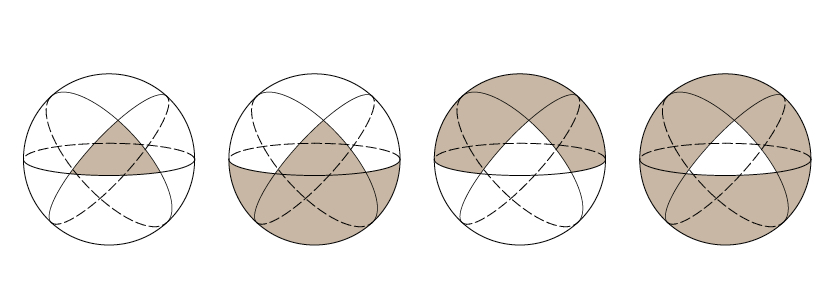
\includegraphics[width=0.9\textwidth]{kugel/Dreieckarten.jpg}
    \captionof{figure}{Dreieckarten auf einer Kugeloberfläche}
\end{center}

Der Begriff Sphärisches Dreieck oder Kugeldreieck ist ein sehr weitläufiger Begriff. 
Dabei können wir den Begriff in drei für uns wesentliche Dreiecke unterteilen:

\begin{itemize}
\item Kugelzweieck
\item Nicht Eulersche’Dreiecke
\item Eulersche’Dreiecke
\end{itemize}

\subsection{Kugelzweieck}

Zwei Grosskreise auf der Kugeloberfläche, zerlegen diese in vier gleiche Kugelzweiecke. 
Jedes dieser Dreieckseiten hat die Länge
$180^{\circ}$ oder $\pi$
Der Flächeninhalt wird dabei nur durch den Winkel $\alpha$ zwischen den beiden Grosskreisen bestimmt.

\begin{center}
        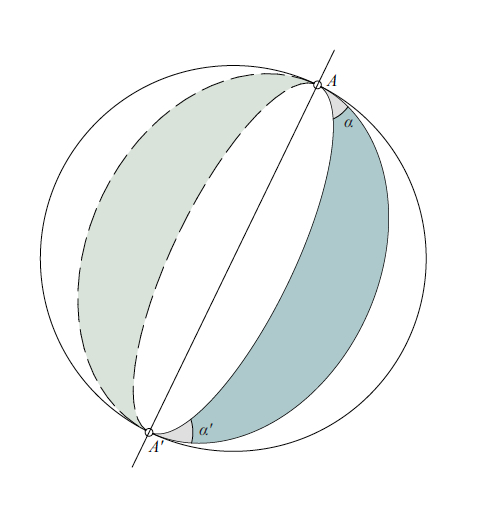
\includegraphics[width=0.3\textwidth]{kugel/Zweieck.jpg}
    \captionof{figure}{Bildung von Zweiecken durch Grosskreise}
\end{center}

Dabei ist der Flächeninhalt der ganzen Kugel:

\begin{align*}
A_{ Kugel } &= 4 \pi r^{2}
\end{align*}


Um den Flächeninhalt des betrachteten Zweieckes zu bekommen, 
müssen wir das ganze noch mit dem Kugelsegment mit dem Winkel $\alpha$ multiplizieren.

\begin{align*}
A_{ Zweieck } &= 4 \pi r^{2} \cdot \frac{ \alpha }{ 2 \pi }
\end{align*}


\subsection{Nicht Eulersche’ Dreiecke}

BLABLA

\subsection{Eulersche’ Dreiecke}

Legt man drei Grosskreise auf eine Kugeloberfläche, bilden sich dabei acht Dreiecke. 
Ein solches Dreieck heisst Eulersches’Dreieck\footnote{%
Leonard Euler (1707-1783), berühmter Schweizer Mathematiker und Physiker. 
Nicht Eulersche’Dreiecke erhält man, indem man das Äussere des Dreieckes ABC betrachtet.} 
Diese Dreiecke werden weder durch die Verlängerung ihrer Seiten durchschnitten, 
noch haben sie Dreiecksseiten welche grösser als $180^{\circ}$ sind.

\begin{center}
        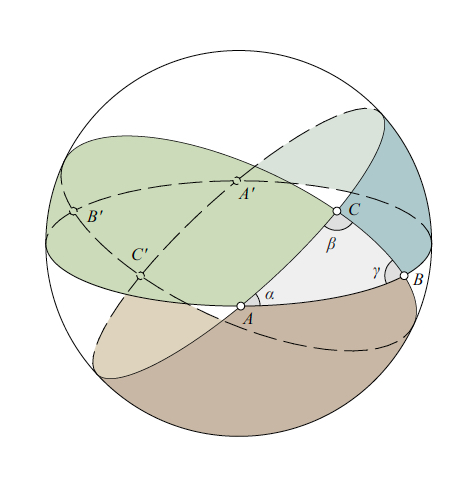
\includegraphics[width=0.4\textwidth]{kugel/Zweiecke.jpg}
    \captionof{figure}{Drei Grosskreise bilden ein sphärisches Dreieck}
\end{center}

In den nachstehenden Erklärungen und Herleitungen, sprechen wir ausschliesslich von Eulerschen’Dreiecken, da die umgeformten Winkelsätze der ebenen Trigonometrie nur auf diese Art von Kugeldreiecken angewendet werden kann.

$A_{ \overline{ ABC }}$ ist die Fläche des Dreieckes auf der Kugeloberfläche
In der ebenen Trigonometrie liegt die Winkelsumme eines Dreiecks bei
$180^{\circ}$.

Anders aber in der sphärischen Trigonometrie. Obschon sie einige Gemeinsamkeiten zur ebenen Trigonometrie aufweist, kann man nicht alles übernehmen.
So auch nicht wie Winkelsumme in einem sphärischen Dreieck.
Diese liegt bei:

\[
\begin{aligned}
\pi
&-
3\pi
&
&\text{\bigg \vert}
&
180^{\circ}
&-
540^{\circ}
\end{aligned}
\]

daraus lässt sich ableiten, das ein einzelner Winkel nicht grösser als $\pi$ oder $180^{\circ}$ sein darf. Ansonsten ist es kein Eulersches’Dreieck und wir dürfen die sphärische Trigonometrie nicht anwenden.\\
Wichtig anzumerken ist, dass die Seiten immer in Radiant beschrieben werden und nicht im Längenmass Meter wie wir es uns gewohnt sind. 
Bei den Dreiecksseiten handelt es sich um Kreisbögen und keine Strecken.

\section{Dreiecksfläche}

\begin{align*}
\text{Zweieck A}
&=
\overline{ABC} + \overline{A'BC} = 2 \alpha r^{ 2 } = A_{ \alpha }\\
\text{Zweieck B}
&=
\overline{ABC} + \overline{AB'C} = 2 \beta r^{ 2 } = A_{ \beta }\\
\text{Zweieck C}
&=
\overline{ABC} + \overline{ABC'} = 2 \gamma r^{ 2 } = A_{ \gamma }
\end{align*}

\begin{align*}
A_{ \alpha } + A_{ \beta } + A_{ \gamma } &= \frac{ 4\pi r^{ 2 } }{ 2 } + 2A_{ \overline{ ABC }} \\
2\alpha r^{ 2 } + 2\beta r^{ 2 } + 2\gamma r^{ 2 } &= \frac{ 4\pi r^{ 2 } }{ 2 } + 2A_{ \overline{ ABC }} \parallel:2\\
\alpha r^{ 2 } + \beta r^{ 2 } + \gamma r^{ 2 } &= \pi r^{ 2 } + A_{ \overline{ ABC }} \parallel-\pi r^{ 2 }\\
r^{ 2 }\left(\alpha + \beta + \gamma - \pi\right) &= A_{ \overline{ ABC }}
\end{align*}




\section{Sphärischer Exzess}
Die Winkelsumme sphärischer Dreiecke ist immer \textgreater \,  $\pi$.

\begin{align*}
\pi < \alpha + \beta + \gamma
\end{align*}

Der sphärische Exzess gibt dabei an, wie stark die Winkelsumme von $\pi$ abweicht.

\begin{align*}
\pi + \epsilon &= \alpha + \beta + \gamma \\
\epsilon &= \alpha + \beta + \gamma - \pi
\end{align*}

Würde der sphärische Exzess in der ebenen Trigonometrie angewendet, wäre dieser = 0. 
Bezieht man das auf die Erde und somit einer Kugel, kann man mit Hilfe eines beliebigen sphärischen Dreieckes und dessen Flächeninhalt auf den Radius der Kugel schliessen.

\subsection{Grenzfall - Satz von Legendre}

\begin{quote} \textit{Ein kleines sphärisches Dreieck kann näherungsweise 
wie ein ebenes Dreieck mit denselben Seiten berechnet 
werden, wenn alle Winkel des ebenen Dreiecks die um 
je ein Drittel des sphärischen Exzesses verminderten 
Winkel des sphärischen Dreiecks nimmt.} \end{quote}
\begin{flushright} - Adrien-Marie Legendre (1752-1833), Paris 1787
\end{flushright}x

Diese Aussage zeigt den Zusammenhang zwischen der 
Trigonometrie in der Ebene sowie in auf der Kugel
auf. Im speziellen bei sehr kleinen sphärischen 
Dreiecken ist die Winkelsumme nur unwesentlich 
grösser als $180^{\circ}$. Des Weiteren kann gesagt werden,
dass der sphärische Exzess gleichmässig auf alle
Winkel aufgeteilt wird.
Wichtig anzumerken ist, dass der Satz von Legendre 
für grosse, aber endliche Radien $r$ gilt.

%[SKIZZE GROSSER RADIUS/KLEINE KRÜMMUNG, KLEINER RADIUS/GROSSE KRÜMMUNG!!!!]
%


\section{Sphärisch Analoge Winkelfunktionen}

\subsection{Sphärischer Sinussatz}

Wir stellen die allgemeinen Sinussätze der Winkel $\alpha$ und $\gamma$ auf:


\[
\begin{aligned}
&{sin(\gamma)} = \frac{h}{a}
&
&\text{\bigg \vert}
&
&{sin(\alpha)} = \frac{h}{c}
&
\end{aligned}
\]

Daraus folgt:
\begin{align*}
h &= sin(\gamma)\cdot a \\
h &= sin(\alpha)\cdot c
\end{align*} 

Durch Gleichsetzung erhält man:
\begin{align*}
h &= h \\
sin(\gamma)\cdot a &= sin(\alpha)\cdot c
\end{align*} 

Durch umstellen erhalten wir den Sinussatz für a und c:
\begin{align*}
sin(\gamma)\cdot a &= sin(\alpha)\cdot c \\
\frac{sin(\gamma)}{c} &= \frac{sin(\alpha)}{a} 
\end{align*} 



\begin{align*}
\frac{sin(\alpha)}{sin(a)} = \frac{sin(\beta)}{sin(b)} = \frac{sin(\gamma)}{sin(c)}
\end{align*} 


\subsection{Winkelkosinussatz}

%[SKIZZE WINKELKOSINUS]

\[
\begin{aligned}
&\overline{C'A'} &= d\cdot {tan(b)}
&
&
&
&
&
&\overline{C'B'} &= d\cdot {tan(a)}
\end{aligned}
\]

\[
\begin{aligned}
&\overline{MA'} &= \frac{ d }{cos(b)}
&
&
&
&
&
&\overline{MB'} &= \frac{ d }{cos(a)}
\end{aligned}
\]

Der allgemeine Kosinussatz beschreibt sich wie folgt:

\begin{align*}
c^{ 2 } &= a^{ 2 } + b^{ 2 } - 2ab \cdot cos(\gamma)
\end{align*}

\begin{align*}
\triangle \overline{A'B'C' }
\overline{ A'B' }^{ 2 } &= \overline{ C'B' }^{ 2 } + \overline{ C'A' }^{ 2 } - 2 \cdot \overline{ C'B' } \cdot \overline{ C'A' } \cdot cos(\gamma)
\end{align*}



\begin{align*}
\overline{A'B'}^{ 2 } &= (d\cdot tan(a))^{ 2 } + (d\cdot tan(b))^{ 2 } - 2 \cdot (d\cdot tan(a) \cdot (d\cdot tan(b) \cdot cos(\gamma)\\
\overline{A'B'}^{ 2 } &= d^{ 2 } \cdot \left(\left(tan^{ 2 }(a) + tan^{ 2 }(b)\right) - 2\cdot tan(a) \cdot tan(b) \cdot cos(\gamma)\right)
\end{align*}

\begin{align*}
\triangle \overline{ MA'B' }
\overline{ A'B' }^{ 2 } &= \overline{ MB' }^{ 2 } + \overline{ MA' }^{ 2 } - 2\cdot \overline{ MB'} \cdot \overline{ MA' } \cdot cos(c)
\end{align*}


\begin{align*}
\overline{ A'B'}^{ 2 } &= \left(\frac{ d }{ cos(a) }  \right)^{ 2 } + \left(\frac{ d }{ cos(b)}  \right)^{ 2 } - 2 \cdot \frac{ d }{ cos(a)} \cdot \frac{ d }{ cos(b)} \cdot cos(c) \\
\overline{ A'B' }^{ 2 } &= d^{ 2 } \cdot \left(\left(\frac{ 1 }{ cos(a) }  \right)^{ 2 } + \left(\frac{ 1 }{ cos(b) }  \right)^{ 2 } - 2 \cdot \frac{ 1 }{ cos(a)} \cdot \frac{ 1 }{ cos(b)} \cdot cos(c)\right)\\
\overline{ A'B' }^{ 2 } &= d^{ 2 } \cdot \left(\left(tan^{ 2 }(a) + 1\right) + \left(tan^{ 2 }(b) + 1\right) - \left(2 \cdot \frac{cos(c)}{cos(a) \cdot cos(b)}\right)\right)
\end{align*}



\begin{align*}
\overline{ A'B'}^{ 2 } &= d^{ 2 } \cdot \left(\left(tan^{ 2 }(a) + tan^{ 2 }(b)\right) - 2 \cdot tan(a) \cdot tan(b) \cdot cos(\gamma)\right) \\
\overline{ A'B'}^{ 2 } &= d^{ 2 } \cdot \left(\left(tan^{ 2 }(a) + 1\right) + \left(tan^{ 2 }(b) + 1\right) - \left(2 \cdot \frac{cos(c)}{cos(a) \cdot cos(b)}\right)\right)
\end{align*}

Die anderen Gleichungen des Satzes, erfolgen aus Symmetriegründen.

\subsection{Seitenkosinussatz}
Durch zyklische Vertauschung des Winkelkosinus erhalten wir den Seitenkosinussatz:

\begin{align*}
{cos(a)} &= {cos(b)} \cdot {cos(c)} + {sin(b)} \cdot {sin(c)} \cdot {sin(\alpha)}\\
{cos(b)} &= {cos(a)} \cdot {cos(c)} + {sin(a)} \cdot {sin(c)} \cdot {sin(\beta)}\\
{cos(c)} &= {cos(a)} \cdot {cos(b)} + {sin(a)} \cdot {sin(b)} \cdot {sin(\gamma)}\\
\end{align*}

\section{Navigation auf See}
Das besondere an Seekarten ist die Inhaltliche Ausrichtung. Anders wie Landkarten muss sie Informationen enthalten welche für den Kapitän und seine Besatzung von grosser Bedeutung sind. Vor allem in Küstennähe ist das navigieren eines Schiffes besonders gefährlich. So enthalten Seekarten etwas über Wassertiefen, Bodenbeschaffenheiten, Gezeiten, Küstenlinien, Landzungen und Windrichtungen.
Der Hauptunterschied dabei ist, das auf der Landkarte feste Positionen definiert und aufgezeigt werden, das einzige was sich verändert ist der Reisende selbst. Bei der Seekarte ist das anders, es werden veränderliche Einwirkungen der Natur festgehalten.

Dieser kleine Unterschied zeigt die Notwendigkeit auf, die Position und den Kurs seines Schiffes auf See immer ermitteln zu können.


\section{Geographische Koordinaten}

Nachdem klar war, das die Erde eine Kugel ist, wurde diese in ein Gradnetz aufgeteilt. Dabei wurden die Angaben für eine exakte Ortsbestimmung klar definiert und die bis heute gültigen Koordinaten bestimmt.
Dabei muss man sich nochmals in Erinnerung rufen, dass sich die Erde in 24h einmal um ihre eigene Achse dreht. Nach $360 ^{\circ}$ 
und somit einer vollen Umdrehung, steht sie wieder in ihrer Ursprungsposition und ein neuer Tag beginnt.

Die Koordinaten setzen sich aus folgenden Komponenten zusammen:

\[
\begin{aligned}
&\text{Grad } (^{\circ})
&
&\text{\bigg \vert}
&
&\text{Bogenminuten } (`)
&
&\text{\bigg \vert}
&
&\text{Bogensekunden } (``)
\end{aligned}
\]

Die Erdoberfläche wurde in je 360 Breiten- und Längengrade eingeteilt. Die Breitengrade haben zueinander einen Abstand von 111.31 km, dies entspricht auch dem Abstand der Längengrade am Äquator mit Zunehmender Nähe zu den Polen, nimmt dieser Abstand ab.

\[
\begin{aligned}
&1^{\circ}
&
&\text{\bigg \vert}
&
&4 \text{ Minuten}
&
&\text{\bigg \vert}
&
&111.31\text{ km}
\end{aligned}
\]

Berechnet man nun die Erdumdrehung von 360°, erhält man genau den Erdumfang am Äquator: \begin{align*} 40’074 \text{ km.}\end{align*}

Dabei geben die Bogenminuten und -sekunden dem Standort die gewünschte Exaktheit. Mit den vollständigen Koordinaten lässt sich der Standort auf einer Landkarte exakt bestimmen und einzeichnen.

\subsection{Zeitzonen der Erde}
Wenn man nun die verschiedenen Zeitzonen der Erde betrachtet, macht die Verschiebung von jeweils einer Stunde durchaus Sinn, es lässt sich auf die Längengrade schliessen.
Zwischen den verschiedenen Zeitzonen liegen 15 Längengrade:

\begin{align*}
\text{15 Längengrade à 4 Minuten = 60 Minuten Zeitverschiebung = ca. 1665 km}
\end{align*}

Dabei ist die Zeitzone in welcher Mitte sich der Greenwich Meredian befindet die \textit{Greenwich Mean Time (GMT)} welche bis 1928 als Weltzeit galt. Im Jahr 1972 wurde diese umbenannt in die \textit{Coordinated Universal Time (UTC)} und wir von da an als Weltzeit $\pm$ 0.00 verwendet.


\section{Der Breitengrad}
Die Breitengrade bilden die bereits genannten Kleinkreise auf der Kugeloberfläche. Sie verlaufen in einem Abstand von genau 111 km parallel zum Äquator. Dabei stellt  dieser genau die Mitte zwischen Nord- und Südpol dar und teilt die Erdkugel in zwei gleiche Hälften. Somit wird von nördlicher und südlicher Breite gesprochen, je nach dem auf welcher Halbkugel man sich befindet.

%[SKIZZE DER GEOGRAFISCHEN BREITE ERDKUGEL]

\subsection{Geografische Breite $\phi$}
\begin{definition}
Die geografische Breite eines Standortes ist nichts anderes, als der Winkel am Erdmittelpunkt zwischen der Ebene des Äquators und der Geraden zum Standpunkt auf der Erdoberfläche.
\end{definition}

%[SKIZZE DER GEOGRAFISCHEN BREITE MIT WINKEL]

\subsection{Navigation mit den Breitengraden}
Da der Breitengrad bereits sehr früh ziemlich präzise bestimmt werden könnte, nutzten bereits die Seefahrer um Christoph Kolumbus den Breitengrad zur Navigation ihrer Flotten.
Den dieser lässt sich ziemlich einfach aus dem höchsten Sonnenstand oder einem Fixstern bestimmen. Dabei wird mit einem Jakobsstab\footnote{%
Der Jakobsstab ist ein früheres astronomisches Instrument zur Winkelmessung und wurde vor allem in der Seefahrt verwendet. Er ist in der Nautik der Vorläufer des Sextanten.} (später Sextant\footnote{%
Der Sextant ist ein nautisches Messinstrument zur Winkelmessung von Horizont und Fixstern (Gestirn)}) der Winkel zwischen dem Horizont und dem Fixstern gemessen. Der Winkel welchen man erhält, zieht man von 90° ab und erhält somit die geografische Breite. \\

%[SKIZZE ERMITTLUNG DES BREITENGRADES]

Wenn man sich auf der Nordhalbkugel befindet, ist der Polarstern ein sehr guter Fixstern. Befindet sich ein Schiff nun sehr nahe am Nordpol, steht dieser nahezu senkrecht am Himmelszelt bei $90^{\circ}$. Würde es aber nahe dem Äquator stehen, erscheint dieser am Horizont bei $0^{\circ}$.

\subsection{Korrekturbeiwert}

\section{Der Längengrad}
Die Längengrade bilden die bereits genannten Grosskreise auf der Kugeloberfläche.
Sie schneiden den Äquator im rechten Winkel, haben dort einen Abstand von 111 km zueinander und verbinden die Pole. Anders wie bei der geografischen Breite, ist in der Natur kein Längengrad gegeben welcher den Nullpunkt darstellt.

%[SKIZZE DER GEOGRAFISCHEN LÄNGE ERDKUGEL]

\subsection{Geografische Länge $\lambda$}
\begin{definition}
Die geografische Länge ist der Winkel an der Erdachse zum Nullmeridian.
\end{definition}

\subsection{Navigation mit den Längengraden}
Die geografische Länge lässt sich nicht so einfach bestimmen wie deren Breite. Für die Berechnung auf See benötigt man eine Referenzzeit eines Ortes mit bekannter Länge.
In der Zeit der Entdecker gab es noch keine mechanischen Uhren. Die Sonnenuhr war zudem ungeeignet, da diese nur die Uhrzeit am Standort mass und nicht die am Referenzort selbst. Die erste Pendeluhr wurde erst Mitte des 17. Jahrhunderts erfunden, was in der Schifffahrt aber auch nicht die Lösung brachte.\\
Pendeluhren auf einem Schiff sind ungeeignet, da das Pendel mit dem Wellengang aus dem Takt gebracht wird und somit die Uhr falsch geht.
Zu ungenau und gegen äussere Erschütterungen zu empfindlich waren später auch die federgetriebenen Uhren und die Unruh. Dazukamen die verschiedenen Klimazonen welche ein Schiff zu durchqueren hatten. Das Metall zog sich viel zu fest zusammen oder dehnte sich aus, was dazu führte das die Uhr unregelmässig lief.

Das sogenannte „Längenproblem“ stellte nicht nur bei der Navigation auf See ein Problem dar, es ergaben sich auch wirtschaftliche Konsequenzen. Die Schiffe mussten bis zur gewünschten geografischen Breite navigieren und segelten dann den Breitengrad entlang. Dabei waren die Schiffe oft Wochenlang unterwegs und segelten die „Breiten ab“ um an die gewünschte Position zu kommen. Dies führte zu erheblichen Zeitverlusten und viel längeren Reisezeiten.


\section{The Board of Longitude - Das Längenproblem}
Das Längenproblem beschäftigte alle grossen Seefahrernationen Europas. Wenn man bedenkt das sich Werte in einer  Höhe von halben britischen Staatshaushalten auf verloren gegangenen Schiffen befanden, erkennt man die Dringlichkeit für eine zuverlässige und genaue Navigation auf See.


\begin{itemize}
\item £ 20’000 - Abweichung von max. einem halben Grad
\item £ 15’000 - Abweichung von zwei Drittel Grad
\item £ 10’000 - Abweichung von max. $1 ^{\circ}$
\end{itemize}

\subsection{John Harrison}


\subsection{Tobias Mayer}



Uhren mit einer Abweichung von einer Minute Abweichung pro Tag (





\section{Nautische Dreieck}


$\Rightarrow$





\section{Die Vermessung der Welt}
Wir schreiben das Jahr 1818 und kehren in die Zeit des Mathematikers Carl Friedrich Gauss zurück. Neben dem liebevoll genannten „kleinen Gauss“ und anderen herausragenden Mathematischen Leistungen, beschäftigte er in den Folgejahren mit der Vermessung des Königreichs Hannovers und verfasste auf 61 Blättern das Kartenwerk \textit{Gauss’sche Landesaufnahme der 1815 durch Hannover erworbenen Gebiete}.






AUFGABE

Hubble Teleskop 
24. April 1990






\printbibliography[heading=subbibliography]
\end{refsection}




%\chapter{Geometrie auf der Kugeloberfläche\label{chapter:kugel}}
\lhead{Geometrie auf der Kugeloberfläche}
\begin{refsection}
\chapterauthor{Melina Staub und Fabian Schmid}

\section{Einleitung}

Schon seit jeher fasziniert den Menschen die Fahrt zur See. Nicht grundlos ist die Seefahrt eine der wichtigsten und ältesten Tätigkeiten der Menschheit. Der innerliche Drang neue Weltmeere und unbekannte Gebiete zu entdecken, die Fahrt zur See zu erleichtern und erträglicher zu machen, trieben die Menschen an, die Schiffe dieser Welt immer weiter zu entwickeln.

Die Idee der Kugelform der Erde ist älter als man zu denken vermag. Bereits der Schüler des antiken griechischen Philosophen Platon - Aristoteles schrieb in seiner Schrift \textit{Über den Himmel} aus dem 4. Jahrhundert v. Chr. etliche Gründe welche für die Gestallt der Erde als Kugel sprechen:

\begin{itemize}
      \item Sämtliche schweren Körper streben zum Mittelpunkt des Alls. Da sie dies von allen Seiten her gleichmäßig tun und die Erde im Mittelpunkt des Alls steht, muss sie eine kugelrunde Gestalt annehmen. 
\item Bei von der Küste wegfahrende Schiffen wird der Rumpf vor den Segeln der Sicht verborgen. 
\item In südlichen Ländern erscheinen südliche Sternbilder höher über dem Horizont.
\item Der Erdschatten bei einer Mondfinsternis ist stets rund.
\end{itemize}

Jedoch war um 1492 - der Zeit der Entdeckung Amerikas durch Christoph Kolumbus, die Idee der Erde in Kugelform noch sehr umstritten. Er erkannte anhand den Theorien und Erkenntnissen der alten Griechen, vor allem Aristoteles, das die Erde eine Kugel sein muss. \\
Doch mit seinem Vorschlag einen Seeweg über den Atlantik nach Indien zu finden und nicht wie üblich um Afrika zu segeln, stiess er beim beim portugiesischen König auf taube Ohren. Sein Plan Indien über eine Route nach Westen zu erreichen, widersprach dem gesunden Menschenverstand. Wäre die Erde wirklich eine Kugel und man befände sich auf der unteren Erdhalbkugel, würde man herunterfallen.\\
Doch auch der damals übliche Glaube an die Erde in Scheibenform brachte so einige Risiken mit sich. Was würde passieren, wenn die Flotte das Ende der Scheibe erreicht hatte? Würden sie über den Erdrand hinweggleiten und in den Abgrund stürzen?\\
Erst nach viel Überzeugungsarbeit durch Kolumbus, setzte er sich am Spanischen Hof durch und segelte über die Westliche Route über den Atlantik und entdeckte schlussendlich Amerika.

Der praktische und greifbare Beweis das die Erde eine Kugel ist, lieferte rund 30 Jahre später der Portugiese Fernando Magellan. Mit seiner Weltumsegelung und seiner Ankunft in den Philippinen, bewies er definitiv das die Erde eine Kugel ist.\\

Nun wollen wir uns die Frage stellen, wie die alten Seefahrer ohne GPS und jeglichen modernen Navigationssystemen auf hoher See wussten wo sie sich befinden und was haben die Sterne mit alldem zu tun? Reisen Sie mit uns zurück in eine Zeit mit Sextant, Kompass und Sternkarten. In die Zeit der Seefahrer und Entdecker.


\section{Geometrie auf der Ebene und der Kugel}

Euklid von Alexandria beschrieb die Grundbegriffe der ebenen Geometrie mittels Punkt, Geraden, Ebene, Winkel und Dreieck. Diese Dreiecke lassen sich mithilfe der ebenen Trigonometrie beschreiben. Dabei gelten die uns bekannten trigonometrischen Winkelfunktionen:\\

\text{Sinussatz:}
\begin{align*}
\frac{ a }{ sin(\alpha) } &= \frac{ b }{sin(\beta)} = \frac{ c }{ sin(\gamma) } = \frac{abc}{2A} = 2r\\
\end{align*}

\text{Cosinussatz:}
\begin{align*}
c^{ 2 } &= a^{ 2 } + b^{ 2 } - 2ab\cdot cos(\gamma)\\
b^{ 2 } &= a^{ 2 } + c^{ 2 } - 2ab\cdot cos(\beta)\\
a^{ 2 } &= b^{ 2 } + c^{ 2 } - 2ab\cdot cos(\alpha)
\end{align*}

Um Dreiecke auf der Kugeloberfläche zu berechnen, benötigt man die sphärische Trigonometrie. Die oben beschriebenen Sätze lassen sich auf der Kugel nicht anwenden, sie werden aber als Grundlage zur Herleitung der Sätze für das Kugeldreieck benötigt.

Die nachfolgenden Seiten thematisieren die Geometrie auf der Kugeloberfläche und wie sie in der Navigation eingesetzt werden kann.


\section{Gross- und Kleinkreise}

Eine Kugeloberfläche lässt sich in zwei verschiedene Kreisarten einteilen -  Gross- und Kleinkreise. 
Wir betrachten als erstes die Grosskreise:

\begin{definition}
Ein Großkreis ist ein größtmöglicher Kreis auf einer Kugeloberfläche. Sein Mittelpunkt fällt immer mit dem Mittelpunkt der Kugel zusammen und ein Schnitt auf dem Großkreis teilt die Kugel in jedem Fall in zwei („gleich große“) Hälften.
\end{definition}

Es gibt unendlich viele Möglichkeiten, eine Kugel in zwei gleich grosse Stücke zu zerschneiden, 
daher gibt es auch unendlich viele Grosskreise. Wenn wir die Grosskreise auf einer Kugel mit diesen auf der Erde beschreiben, sprechen wir von den Längengraden aber auch der Äquator beschreibt einen Grosskreis.
Ein Elementarer Bestandteil bilden die Grosskreise in der sphärischen Trigonometrie. Mithilfe der Schnittpunkte verschiedener Grosskreise, lässt sich ein Sphärisches Dreieck bilden auf welchem sich die sphärische Trigonometrie anwenden lässt.

[GRAFIK GROSSKREISE]

\begin{definition}
Unter Kleinkreis versteht man jene Kreise auf einer Kugeloberfläche, deren Ebenen nicht den Kugelmittelpunkt enthalten.
\end{definition}

Die Kleinkreise eignen sich im Gegensatz zu den Grosskreisen \textit{nicht} für die sphärische Trigonometrie. 
Sie werden lediglich zur Bestimmung der Messgrössen, Winkelabstände oder des Höhenwinkels eines Gestirns verwendet. 

Wenn wir die Kleinkreise auf die Erdoberfläche projizieren betrachten wir die Breitengrade.

[GRAFIK KLEINKREISE]


\section{Sphärische Dreiecke / Kugeldreieck}

\begin{center}
        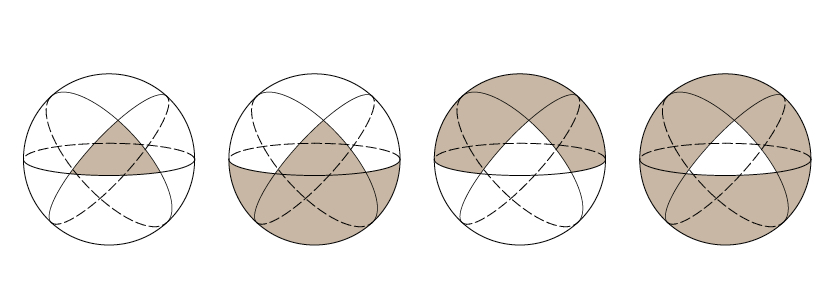
\includegraphics[width=0.9\textwidth]{kugel/Dreieckarten.jpg}
    \captionof{figure}{Dreieckarten auf einer Kugeloberfläche}
\end{center}

Der Begriff Sphärisches Dreieck oder Kugeldreieck ist ein sehr weitläufiger Begriff. 
Dabei können wir den Begriff in drei für uns wesentliche Dreiecke unterteilen:

\begin{itemize}
\item Kugelzweieck
\item Nicht Eulersche’Dreiecke
\item Eulersche’Dreiecke
\end{itemize}

\subsection{Kugelzweieck}

Zwei Grosskreise auf der Kugeloberfläche, zerlegen diese in vier gleiche Kugelzweiecke. 
Jedes dieser Dreieckseiten hat die Länge
$180^{\circ}$ oder $\pi$
Der Flächeninhalt wird dabei nur durch den Winkel $\alpha$ zwischen den beiden Grosskreisen bestimmt.

\begin{center}
        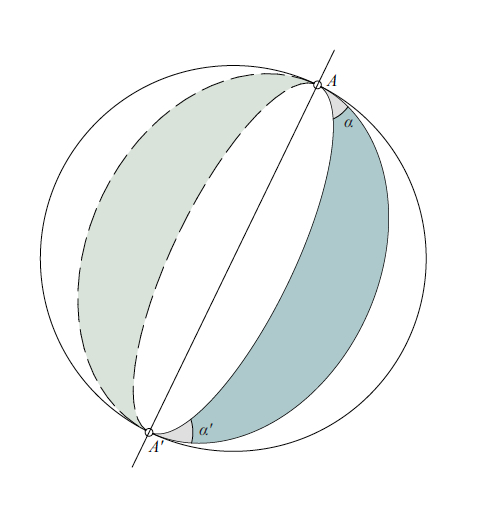
\includegraphics[width=0.3\textwidth]{kugel/Zweieck.jpg}
    \captionof{figure}{Bildung von Zweiecken durch Grosskreise}
\end{center}

Dabei ist der Flächeninhalt der ganzen Kugel:

\begin{align*}
A_{ Kugel } &= 4 \pi r^{2}
\end{align*}


Um den Flächeninhalt des betrachteten Zweieckes zu bekommen, 
müssen wir das ganze noch mit dem Kugelsegment mit dem Winkel $\alpha$ multiplizieren.

\begin{align*}
A_{ Zweieck } &= 4 \pi r^{2} \cdot \frac{ \alpha }{ 2 \pi }
\end{align*}


\subsection{Nicht Eulersche’ Dreiecke}

BLABLA

\subsection{Eulersche’ Dreiecke}

Legt man drei Grosskreise auf eine Kugeloberfläche, bilden sich dabei acht Dreiecke. 
Ein solches Dreieck heisst Eulersches’Dreieck\footnote{%
Leonard Euler (1707-1783), berühmter Schweizer Mathematiker und Physiker. 
Nicht Eulersche’Dreiecke erhält man, indem man das Äussere des Dreieckes ABC betrachtet.} 
Diese Dreiecke werden weder durch die Verlängerung ihrer Seiten durchschnitten, 
noch haben sie Dreiecksseiten welche grösser als $180^{\circ}$ sind.

\begin{center}
        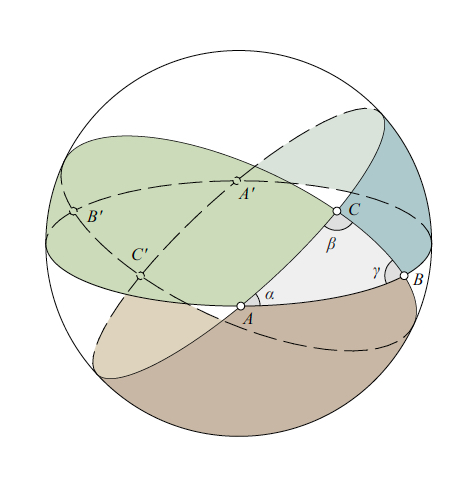
\includegraphics[width=0.4\textwidth]{kugel/Zweiecke.jpg}
    \captionof{figure}{Drei Grosskreise bilden ein sphärisches Dreieck}
\end{center}

In den nachstehenden Erklärungen und Herleitungen, sprechen wir ausschliesslich von Eulerschen’Dreiecken, da die umgeformten Winkelsätze der ebenen Trigonometrie nur auf diese Art von Kugeldreiecken angewendet werden kann.

$A_{ \overline{ ABC }}$ ist die Fläche des Dreieckes auf der Kugeloberfläche
In der ebenen Trigonometrie liegt die Winkelsumme eines Dreiecks bei
$180^{\circ}$.

Anders aber in der sphärischen Trigonometrie. Obschon sie einige Gemeinsamkeiten zur ebenen Trigonometrie aufweist, kann man nicht alles übernehmen.
So auch nicht wie Winkelsumme in einem sphärischen Dreieck.
Diese liegt bei:

\[
\begin{aligned}
\pi
&-
3\pi
&
&\text{\bigg \vert}
&
180^{\circ}
&-
540^{\circ}
\end{aligned}
\]

daraus lässt sich ableiten, das ein einzelner Winkel nicht grösser als $\pi$ oder $180^{\circ}$ sein darf. Ansonsten ist es kein Eulersches’Dreieck und wir dürfen die sphärische Trigonometrie nicht anwenden.\\
Wichtig anzumerken ist, dass die Seiten immer in Radiant beschrieben werden und nicht im Längenmass Meter wie wir es uns gewohnt sind. 
Bei den Dreiecksseiten handelt es sich um Kreisbögen und keine Strecken.

\section{Dreiecksfläche}

\begin{align*}
\text{Zweieck A}
&=
\overline{ABC} + \overline{A'BC} = 2 \alpha r^{ 2 } = A_{ \alpha }\\
\text{Zweieck B}
&=
\overline{ABC} + \overline{AB'C} = 2 \beta r^{ 2 } = A_{ \beta }\\
\text{Zweieck C}
&=
\overline{ABC} + \overline{ABC'} = 2 \gamma r^{ 2 } = A_{ \gamma }
\end{align*}

\begin{align*}
A_{ \alpha } + A_{ \beta } + A_{ \gamma } &= \frac{ 4\pi r^{ 2 } }{ 2 } + 2A_{ \overline{ ABC }} \\
2\alpha r^{ 2 } + 2\beta r^{ 2 } + 2\gamma r^{ 2 } &= \frac{ 4\pi r^{ 2 } }{ 2 } + 2A_{ \overline{ ABC }} \parallel:2\\
\alpha r^{ 2 } + \beta r^{ 2 } + \gamma r^{ 2 } &= \pi r^{ 2 } + A_{ \overline{ ABC }} \parallel-\pi r^{ 2 }\\
r^{ 2 }\left(\alpha + \beta + \gamma - \pi\right) &= A_{ \overline{ ABC }}
\end{align*}




\section{Sphärischer Exzess}
Die Winkelsumme sphärischer Dreiecke ist immer \textgreater \,  $\pi$.

\begin{align*}
\pi < \alpha + \beta + \gamma
\end{align*}

Der sphärische Exzess gibt dabei an, wie stark die Winkelsumme von $\pi$ abweicht.

\begin{align*}
\pi + \epsilon &= \alpha + \beta + \gamma \\
\epsilon &= \alpha + \beta + \gamma - \pi
\end{align*}

Würde der sphärische Exzess in der ebenen Trigonometrie angewendet, wäre dieser = 0. 
Bezieht man das auf die Erde und somit einer Kugel, kann man mit Hilfe eines beliebigen sphärischen Dreieckes und dessen Flächeninhalt auf den Radius der Kugel schliessen.

\subsection{Grenzfall - Satz von Legendre}

\begin{quote} \textit{Ein kleines sphärisches Dreieck kann näherungsweise 
wie ein ebenes Dreieck mit denselben Seiten berechnet 
werden, wenn alle Winkel des ebenen Dreiecks die um 
je ein Drittel des sphärischen Exzesses verminderten 
Winkel des sphärischen Dreiecks nimmt.} \end{quote}
\begin{flushright} - Adrien-Marie Legendre (1752-1833), Paris 1787
\end{flushright}x

Diese Aussage zeigt den Zusammenhang zwischen der 
Trigonometrie in der Ebene sowie in auf der Kugel
auf. Im speziellen bei sehr kleinen sphärischen 
Dreiecken ist die Winkelsumme nur unwesentlich 
grösser als $180^{\circ}$. Des Weiteren kann gesagt werden,
dass der sphärische Exzess gleichmässig auf alle
Winkel aufgeteilt wird.
Wichtig anzumerken ist, dass der Satz von Legendre 
für grosse, aber endliche Radien $r$ gilt.

%[SKIZZE GROSSER RADIUS/KLEINE KRÜMMUNG, KLEINER RADIUS/GROSSE KRÜMMUNG!!!!]
%


\section{Sphärisch Analoge Winkelfunktionen}

\subsection{Sphärischer Sinussatz}

Wir stellen die allgemeinen Sinussätze der Winkel $\alpha$ und $\gamma$ auf:


\[
\begin{aligned}
&{sin(\gamma)} = \frac{h}{a}
&
&\text{\bigg \vert}
&
&{sin(\alpha)} = \frac{h}{c}
&
\end{aligned}
\]

Daraus folgt:
\begin{align*}
h &= sin(\gamma)\cdot a \\
h &= sin(\alpha)\cdot c
\end{align*} 

Durch Gleichsetzung erhält man:
\begin{align*}
h &= h \\
sin(\gamma)\cdot a &= sin(\alpha)\cdot c
\end{align*} 

Durch umstellen erhalten wir den Sinussatz für a und c:
\begin{align*}
sin(\gamma)\cdot a &= sin(\alpha)\cdot c \\
\frac{sin(\gamma)}{c} &= \frac{sin(\alpha)}{a} 
\end{align*} 



\begin{align*}
\frac{sin(\alpha)}{sin(a)} = \frac{sin(\beta)}{sin(b)} = \frac{sin(\gamma)}{sin(c)}
\end{align*} 


\subsection{Winkelkosinussatz}

%[SKIZZE WINKELKOSINUS]

\[
\begin{aligned}
&\overline{C'A'} &= d\cdot {tan(b)}
&
&
&
&
&
&\overline{C'B'} &= d\cdot {tan(a)}
\end{aligned}
\]

\[
\begin{aligned}
&\overline{MA'} &= \frac{ d }{cos(b)}
&
&
&
&
&
&\overline{MB'} &= \frac{ d }{cos(a)}
\end{aligned}
\]

Der allgemeine Kosinussatz beschreibt sich wie folgt:

\begin{align*}
c^{ 2 } &= a^{ 2 } + b^{ 2 } - 2ab \cdot cos(\gamma)
\end{align*}

\begin{align*}
\triangle \overline{A'B'C' }
\overline{ A'B' }^{ 2 } &= \overline{ C'B' }^{ 2 } + \overline{ C'A' }^{ 2 } - 2 \cdot \overline{ C'B' } \cdot \overline{ C'A' } \cdot cos(\gamma)
\end{align*}



\begin{align*}
\overline{A'B'}^{ 2 } &= (d\cdot tan(a))^{ 2 } + (d\cdot tan(b))^{ 2 } - 2 \cdot (d\cdot tan(a) \cdot (d\cdot tan(b) \cdot cos(\gamma)\\
\overline{A'B'}^{ 2 } &= d^{ 2 } \cdot \left(\left(tan^{ 2 }(a) + tan^{ 2 }(b)\right) - 2\cdot tan(a) \cdot tan(b) \cdot cos(\gamma)\right)
\end{align*}

\begin{align*}
\triangle \overline{ MA'B' }
\overline{ A'B' }^{ 2 } &= \overline{ MB' }^{ 2 } + \overline{ MA' }^{ 2 } - 2\cdot \overline{ MB'} \cdot \overline{ MA' } \cdot cos(c)
\end{align*}


\begin{align*}
\overline{ A'B'}^{ 2 } &= \left(\frac{ d }{ cos(a) }  \right)^{ 2 } + \left(\frac{ d }{ cos(b)}  \right)^{ 2 } - 2 \cdot \frac{ d }{ cos(a)} \cdot \frac{ d }{ cos(b)} \cdot cos(c) \\
\overline{ A'B' }^{ 2 } &= d^{ 2 } \cdot \left(\left(\frac{ 1 }{ cos(a) }  \right)^{ 2 } + \left(\frac{ 1 }{ cos(b) }  \right)^{ 2 } - 2 \cdot \frac{ 1 }{ cos(a)} \cdot \frac{ 1 }{ cos(b)} \cdot cos(c)\right)\\
\overline{ A'B' }^{ 2 } &= d^{ 2 } \cdot \left(\left(tan^{ 2 }(a) + 1\right) + \left(tan^{ 2 }(b) + 1\right) - \left(2 \cdot \frac{cos(c)}{cos(a) \cdot cos(b)}\right)\right)
\end{align*}



\begin{align*}
\overline{ A'B'}^{ 2 } &= d^{ 2 } \cdot \left(\left(tan^{ 2 }(a) + tan^{ 2 }(b)\right) - 2 \cdot tan(a) \cdot tan(b) \cdot cos(\gamma)\right) \\
\overline{ A'B'}^{ 2 } &= d^{ 2 } \cdot \left(\left(tan^{ 2 }(a) + 1\right) + \left(tan^{ 2 }(b) + 1\right) - \left(2 \cdot \frac{cos(c)}{cos(a) \cdot cos(b)}\right)\right)
\end{align*}

Die anderen Gleichungen des Satzes, erfolgen aus Symmetriegründen.

\subsection{Seitenkosinussatz}
Durch zyklische Vertauschung des Winkelkosinus erhalten wir den Seitenkosinussatz:

\begin{align*}
{cos(a)} &= {cos(b)} \cdot {cos(c)} + {sin(b)} \cdot {sin(c)} \cdot {sin(\alpha)}\\
{cos(b)} &= {cos(a)} \cdot {cos(c)} + {sin(a)} \cdot {sin(c)} \cdot {sin(\beta)}\\
{cos(c)} &= {cos(a)} \cdot {cos(b)} + {sin(a)} \cdot {sin(b)} \cdot {sin(\gamma)}\\
\end{align*}

\section{Navigation auf See}
Das besondere an Seekarten ist die Inhaltliche Ausrichtung. Anders wie Landkarten muss sie Informationen enthalten welche für den Kapitän und seine Besatzung von grosser Bedeutung sind. Vor allem in Küstennähe ist das navigieren eines Schiffes besonders gefährlich. So enthalten Seekarten etwas über Wassertiefen, Bodenbeschaffenheiten, Gezeiten, Küstenlinien, Landzungen und Windrichtungen.
Der Hauptunterschied dabei ist, das auf der Landkarte feste Positionen definiert und aufgezeigt werden, das einzige was sich verändert ist der Reisende selbst. Bei der Seekarte ist das anders, es werden veränderliche Einwirkungen der Natur festgehalten.

Dieser kleine Unterschied zeigt die Notwendigkeit auf, die Position und den Kurs seines Schiffes auf See immer ermitteln zu können.


\section{Geographische Koordinaten}

Nachdem klar war, das die Erde eine Kugel ist, wurde diese in ein Gradnetz aufgeteilt. Dabei wurden die Angaben für eine exakte Ortsbestimmung klar definiert und die bis heute gültigen Koordinaten bestimmt.
Dabei muss man sich nochmals in Erinnerung rufen, dass sich die Erde in 24h einmal um ihre eigene Achse dreht. Nach $360 ^{\circ}$ 
und somit einer vollen Umdrehung, steht sie wieder in ihrer Ursprungsposition und ein neuer Tag beginnt.

Die Koordinaten setzen sich aus folgenden Komponenten zusammen:

\[
\begin{aligned}
&\text{Grad } (^{\circ})
&
&\text{\bigg \vert}
&
&\text{Bogenminuten } (`)
&
&\text{\bigg \vert}
&
&\text{Bogensekunden } (``)
\end{aligned}
\]

Die Erdoberfläche wurde in je 360 Breiten- und Längengrade eingeteilt. Die Breitengrade haben zueinander einen Abstand von 111.31 km, dies entspricht auch dem Abstand der Längengrade am Äquator mit Zunehmender Nähe zu den Polen, nimmt dieser Abstand ab.

\[
\begin{aligned}
&1^{\circ}
&
&\text{\bigg \vert}
&
&4 \text{ Minuten}
&
&\text{\bigg \vert}
&
&111.31\text{ km}
\end{aligned}
\]

Berechnet man nun die Erdumdrehung von 360°, erhält man genau den Erdumfang am Äquator: \begin{align*} 40’074 \text{ km.}\end{align*}

Dabei geben die Bogenminuten und -sekunden dem Standort die gewünschte Exaktheit. Mit den vollständigen Koordinaten lässt sich der Standort auf einer Landkarte exakt bestimmen und einzeichnen.

\subsection{Zeitzonen der Erde}
Wenn man nun die verschiedenen Zeitzonen der Erde betrachtet, macht die Verschiebung von jeweils einer Stunde durchaus Sinn, es lässt sich auf die Längengrade schliessen.
Zwischen den verschiedenen Zeitzonen liegen 15 Längengrade:

\begin{align*}
\text{15 Längengrade à 4 Minuten = 60 Minuten Zeitverschiebung = ca. 1665 km}
\end{align*}

Dabei ist die Zeitzone in welcher Mitte sich der Greenwich Meredian befindet die \textit{Greenwich Mean Time (GMT)} welche bis 1928 als Weltzeit galt. Im Jahr 1972 wurde diese umbenannt in die \textit{Coordinated Universal Time (UTC)} und wir von da an als Weltzeit $\pm$ 0.00 verwendet.


\section{Der Breitengrad}
Die Breitengrade bilden die bereits genannten Kleinkreise auf der Kugeloberfläche. Sie verlaufen in einem Abstand von genau 111 km parallel zum Äquator. Dabei stellt  dieser genau die Mitte zwischen Nord- und Südpol dar und teilt die Erdkugel in zwei gleiche Hälften. Somit wird von nördlicher und südlicher Breite gesprochen, je nach dem auf welcher Halbkugel man sich befindet.

%[SKIZZE DER GEOGRAFISCHEN BREITE ERDKUGEL]

\subsection{Geografische Breite $\phi$}
\begin{definition}
Die geografische Breite eines Standortes ist nichts anderes, als der Winkel am Erdmittelpunkt zwischen der Ebene des Äquators und der Geraden zum Standpunkt auf der Erdoberfläche.
\end{definition}

%[SKIZZE DER GEOGRAFISCHEN BREITE MIT WINKEL]

\subsection{Navigation mit den Breitengraden}
Da der Breitengrad bereits sehr früh ziemlich präzise bestimmt werden könnte, nutzten bereits die Seefahrer um Christoph Kolumbus den Breitengrad zur Navigation ihrer Flotten.
Den dieser lässt sich ziemlich einfach aus dem höchsten Sonnenstand oder einem Fixstern bestimmen. Dabei wird mit einem Jakobsstab\footnote{%
Der Jakobsstab ist ein früheres astronomisches Instrument zur Winkelmessung und wurde vor allem in der Seefahrt verwendet. Er ist in der Nautik der Vorläufer des Sextanten.} (später Sextant\footnote{%
Der Sextant ist ein nautisches Messinstrument zur Winkelmessung von Horizont und Fixstern (Gestirn)}) der Winkel zwischen dem Horizont und dem Fixstern gemessen. Der Winkel welchen man erhält, zieht man von 90° ab und erhält somit die geografische Breite. \\

%[SKIZZE ERMITTLUNG DES BREITENGRADES]

Wenn man sich auf der Nordhalbkugel befindet, ist der Polarstern ein sehr guter Fixstern. Befindet sich ein Schiff nun sehr nahe am Nordpol, steht dieser nahezu senkrecht am Himmelszelt bei $90^{\circ}$. Würde es aber nahe dem Äquator stehen, erscheint dieser am Horizont bei $0^{\circ}$.

\subsection{Korrekturbeiwert}

\section{Der Längengrad}
Die Längengrade bilden die bereits genannten Grosskreise auf der Kugeloberfläche.
Sie schneiden den Äquator im rechten Winkel, haben dort einen Abstand von 111 km zueinander und verbinden die Pole. Anders wie bei der geografischen Breite, ist in der Natur kein Längengrad gegeben welcher den Nullpunkt darstellt.

%[SKIZZE DER GEOGRAFISCHEN LÄNGE ERDKUGEL]

\subsection{Geografische Länge $\lambda$}
\begin{definition}
Die geografische Länge ist der Winkel an der Erdachse zum Nullmeridian.
\end{definition}

\subsection{Navigation mit den Längengraden}
Die geografische Länge lässt sich nicht so einfach bestimmen wie deren Breite. Für die Berechnung auf See benötigt man eine Referenzzeit eines Ortes mit bekannter Länge.
In der Zeit der Entdecker gab es noch keine mechanischen Uhren. Die Sonnenuhr war zudem ungeeignet, da diese nur die Uhrzeit am Standort mass und nicht die am Referenzort selbst. Die erste Pendeluhr wurde erst Mitte des 17. Jahrhunderts erfunden, was in der Schifffahrt aber auch nicht die Lösung brachte.\\
Pendeluhren auf einem Schiff sind ungeeignet, da das Pendel mit dem Wellengang aus dem Takt gebracht wird und somit die Uhr falsch geht.
Zu ungenau und gegen äussere Erschütterungen zu empfindlich waren später auch die federgetriebenen Uhren und die Unruh. Dazukamen die verschiedenen Klimazonen welche ein Schiff zu durchqueren hatten. Das Metall zog sich viel zu fest zusammen oder dehnte sich aus, was dazu führte das die Uhr unregelmässig lief.

Das sogenannte „Längenproblem“ stellte nicht nur bei der Navigation auf See ein Problem dar, es ergaben sich auch wirtschaftliche Konsequenzen. Die Schiffe mussten bis zur gewünschten geografischen Breite navigieren und segelten dann den Breitengrad entlang. Dabei waren die Schiffe oft Wochenlang unterwegs und segelten die „Breiten ab“ um an die gewünschte Position zu kommen. Dies führte zu erheblichen Zeitverlusten und viel längeren Reisezeiten.


\section{The Board of Longitude - Das Längenproblem}
Das Längenproblem beschäftigte alle grossen Seefahrernationen Europas. Wenn man bedenkt das sich Werte in einer  Höhe von halben britischen Staatshaushalten auf verloren gegangenen Schiffen befanden, erkennt man die Dringlichkeit für eine zuverlässige und genaue Navigation auf See.


\begin{itemize}
\item £ 20’000 - Abweichung von max. einem halben Grad
\item £ 15’000 - Abweichung von zwei Drittel Grad
\item £ 10’000 - Abweichung von max. $1 ^{\circ}$
\end{itemize}

\subsection{John Harrison}


\subsection{Tobias Mayer}



Uhren mit einer Abweichung von einer Minute Abweichung pro Tag (





\section{Nautische Dreieck}


$\Rightarrow$





\section{Die Vermessung der Welt}
Wir schreiben das Jahr 1818 und kehren in die Zeit des Mathematikers Carl Friedrich Gauss zurück. Neben dem liebevoll genannten „kleinen Gauss“ und anderen herausragenden Mathematischen Leistungen, beschäftigte er in den Folgejahren mit der Vermessung des Königreichs Hannovers und verfasste auf 61 Blättern das Kartenwerk \textit{Gauss’sche Landesaufnahme der 1815 durch Hannover erworbenen Gebiete}.






AUFGABE

Hubble Teleskop 
24. April 1990






\printbibliography[heading=subbibliography]
\end{refsection}




\vfill
\pagebreak
\ifodd\value{page}\else\null\clearpage\fi
\lhead{Index}
\rhead{}
\addcontentsline{toc}{chapter}{\indexname}
%
% skript.tex -- Skript ueber Differentialgleichungen
%
% (c) 2014 Prof. Dr. Andreas Mueller, HSR
%
\documentclass{book}
\usepackage{etex}
\usepackage{geometry}
\geometry{papersize={170mm,240mm},total={140mm,200mm},top=21mm,bindingoffset=10mm}
\usepackage[english,ngerman]{babel}
\usepackage[utf8]{inputenc}
\usepackage{cancel}
\usepackage{times}
\usepackage{amsmath,amscd}
\usepackage{amssymb}
\usepackage{amsfonts}
\usepackage{amsthm}
\usepackage[nolist]{acronym}
\usepackage{graphicx}
\usepackage{fancyhdr}
\usepackage{textcomp}
\usepackage[all]{xy}
\usepackage{txfonts}
\usepackage{alltt} 
\usepackage{verbatim}
\usepackage{paralist}
\usepackage{makeidx}
\usepackage{array}
%\usepackage[colorlinks=true]{hyperref}
\usepackage{hyperref}
\usepackage{tikz}
\usepackage{pgfplots}
\usepackage{pgfplotstable}
\usepackage{pdftexcmds}
%\usepackage{pgfmath}
\usepackage{placeins}
\usepackage{subfigure}
\usepackage[autostyle=false,english=american]{csquotes}
\usepackage{float}
\usepackage{enumitem}
\usepackage{wasysym}
\usepackage{environ}
\usepackage{pifont}
\usepackage{feynmp}
\usepackage{appendix}
\usetikzlibrary{calc,intersections,through,backgrounds,graphs,positioning,shapes,arrows,fit}
\usetikzlibrary{patterns,decorations.pathreplacing}
\usetikzlibrary{decorations.pathreplacing}
\usetikzlibrary{external}
\usepackage[europeanvoltages,
            europeancurrents,
            europeanresistors,   % rectangular shape
            americaninductors,   % "4-bumbs" shape
            europeanports,       % rectangular logic ports
            siunitx,             % #1<#2>
            emptydiodes,
            noarrowmos,
            smartlabels]         % lables are rotated in a smart way
           {circuitikz}          %
\usepackage{siunitx}
\usepackage{tabularx}
\usetikzlibrary{arrows}

\usepackage{algpseudocode}
\usepackage{algorithm}

% Matlab
\usepackage{listings}
\usepackage{color} %red, green, blue, yellow, cyan, magenta, black, white
\definecolor{mygreen}{RGB}{28,172,0} % color values Red, Green, Blue
\definecolor{mylilas}{RGB}{170,55,241}

\lstset{language=Matlab,%
    %basicstyle=\color{red},
    breaklines=true,%
    morekeywords={matlab2tikz},
    keywordstyle=\color{blue},%
    morekeywords=[2]{1}, keywordstyle=[2]{\color{black}},
    identifierstyle=\color{black},%
    stringstyle=\color{mylilas},
    commentstyle=\color{mygreen},%
    showstringspaces=false,%without this there will be a symbol in the places where there is a space
    numbers=left,%
    %numberstyle={\tiny \color{black}},% size of the numbers
    numbersep=9pt, % this defines how far the numbers are from the text
    emph=[1]{break},emphstyle=[1]\color{red}, %some words to emphasise
    %emph=[2]{word1,word2}, emphstyle=[2]{style},    
}
\lstdefinestyle{Matlab}{
  numbers=left,
  belowcaptionskip=1\baselineskip,
  breaklines=true,
  frame=L,
  xleftmargin=\parindent,
  language=Matlab,
  showstringspaces=false,
  basicstyle=\footnotesize\ttfamily,
  keywordstyle=\bfseries\color{green!40!black},
  commentstyle=\itshape\color{purple!40!black},
  identifierstyle=\color{blue},
  stringstyle=\color{orange},
  numberstyle=\ttfamily\tiny
}
\lstdefinelanguage{Maxima}{
  keywords={addrow,addcol,zeromatrix,ident,augcoefmatrix,ratsubst,sum,diff,ev,tex,%
    with_stdout,nouns,express,depends,load,length,submatrix,div,grad,curl,matrix,%
    invert,lambda,facsum,expand,false,then,if,else,subst,%
    rootscontract,solve,part,assume,sqrt,integrate,abs,inf,exp,sin,cos,sinh,cosh},
  sensitive=true,
  comment=[n][\itshape]{/*}{*/}
}
\lstdefinestyle{Maxima}{
  numbers=left,
  belowcaptionskip=1\baselineskip,
  breaklines=true,
  frame=L,
  xleftmargin=\parindent,
  language=Maxima,
  showstringspaces=false,
  basicstyle=\footnotesize\ttfamily,
  keywordstyle=\bfseries\color{green!40!black},
  commentstyle=\itshape\color{purple!40!black},
  identifierstyle=\color{blue},
  stringstyle=\color{orange},
  numberstyle=\ttfamily\tiny
}
\lstdefinestyle{Octave}{
  numbers=left,
  belowcaptionskip=1\baselineskip,
  breaklines=true,
  frame=L,
  xleftmargin=\parindent,
  language=Octave,
  showstringspaces=false,
  basicstyle=\footnotesize\ttfamily,
  keywordstyle=\bfseries\color{green!40!black},
  commentstyle=\itshape\color{purple!40!black},
  identifierstyle=\color{blue},
  stringstyle=\color{orange},
  numberstyle=\ttfamily\tiny
}
\lstdefinestyle{C}{
  numbers=left,
  belowcaptionskip=1\baselineskip,
  breaklines=true,
  frame=L,
  xleftmargin=\parindent,
  language=C,
  showstringspaces=false,
  basicstyle=\footnotesize\ttfamily,
  keywordstyle=\bfseries\color{green!40!black},
  commentstyle=\itshape\color{purple!40!black},
  identifierstyle=\color{blue},
  stringstyle=\color{orange},
  numberstyle=\ttfamily\tiny
}
\usepackage{caption}
\usepackage[mode=buildnew]{standalone}
\usepackage[backend=bibtex]{biblatex}
% workaround for biblatex bug
\makeatletter
\def\blx@maxline{77}
\makeatother
\addbibresource{references.bib}
% Bibresources für jeden einzelnen Artikel
%\addbibresource{friedmann/main.bib}
%\addbibresource{komplex/main.bib}
%\addbibresource{kreis/main.bib}
%\addbibresource{licht/main.bib}
%\addbibresource{schrittlaenge/main.bib}
%\addbibresource{sir/main.bib}
%\addbibresource{trafo/main.bib}
%\addbibresource{wellen/main.bib}
\AtEndDocument{\clearpage\ifodd\value{page}\else\null\clearpage\fi}
\makeindex
%\pgfplotsset{compat=1.12}
\setlength{\headheight}{15pt} % fix headheight warning
\DeclareGraphicsRule{*}{mps}{*}{}
\begin{document}
\pagestyle{fancy}
\frontmatter
\newcommand\HRule{\noindent\rule{\linewidth}{1.5pt}}
\begin{titlepage}
\vspace*{\stretch{1}}
\HRule
\vspace*{5pt}
\begin{flushright}
{
\LARGE
Mathematisches Seminar\\
\vspace*{20pt}
\Huge
Kosmologie%
}
\vspace*{5pt}
\end{flushright}
\HRule
\begin{flushright}
\vspace{60pt}
\Large
Leitung: Andreas M"uller\\
\vspace{40pt}
\Large
%Reto~Christen,
%Kevin~Cina,
%Andri~Hartmann,
%Pascal~Horat %,
%Matthias~Kn"opfel,
%Stefan Kull,
%Daniela~Meier,
%Max~Obrist %,
%Hansruedi~Patzen,
%Benjamin~R"aber,
%Simon~Schaefer %,
%Tibor~Schneider,
%Tobias~Schuler,
%Roy~Seitz,
%Martin~Stypinski
\end{flushright}
\vspace*{\stretch{2}}
\begin{center}
Hochschule f"ur Technik, Rapperswil, 2017
\end{center}
\end{titlepage}
\hypersetup{
    linktoc=all,
    linkcolor=blue
}
\newcounter{beispiel}
\newenvironment{beispiele}{
\bgroup\smallskip\parindent0pt\bf Beispiele\egroup

\begin{list}{\arabic{beispiel}.}
  {\usecounter{beispiel}
  \setlength{\labelsep}{5mm}
  \setlength{\rightmargin}{0pt}
}}{\end{list}}
\newcounter{uebungsaufgabezaehler}
% environment fuer uebungsaufgaben
\newenvironment{uebungsaufgaben}{
\begin{list}{\arabic{uebungsaufgabezaehler}.}
  {\usecounter{uebungsaufgabezaehler}
  \setlength{\labelwidth}{2cm}
  \setlength{\leftmargin}{0pt}
  \setlength{\labelsep}{5mm}
  \setlength{\rightmargin}{0pt}
  \setlength{\itemindent}{0pt}
}}{\end{list}\vfill\pagebreak}
\newenvironment{teilaufgaben}{
\begin{enumerate}
\renewcommand{\labelenumi}{\alph{enumi})}
}{\end{enumerate}}
% Aufgabe
\newcounter{problemcounter}[chapter]
\def\aufgabepath{uebungsaufgaben/}
\def\ainput#1{\input\aufgabepath/#1}
\def\verbatimainput#1{\expandafter\verbatiminput{\aufgabepath/#1}}
\def\aufgabetoplevel#1{%
\expandafter\def\expandafter\inputpath{#1}%
\let\aufgabepath=\inputpath
}
\def\includeagraphics[#1]#2{\expandafter\includegraphics[#1]{\aufgabepath#2}}
% \aufgabe
\newcommand{\uebungsaufgabe}[1]{%
\refstepcounter{problemcounter}%
\label{#1}%
\bigskip{\parindent0pt\strut}\hbox{\bf\arabic{problemcounter}. }%
\expandafter\def\csname aufgabepath\endcsname{\inputpath/}%
\expandafter\input{uebungsaufgaben/#1.tex}
}
\renewcommand\theproblemcounter{\thechapter.\arabic{problemcounter}}

% Loesung
\def\swallow#1{
%nothing
}
\NewEnviron{loesung}[1][L"osung]{%
\begin{proof}[#1]%
\renewcommand{\qedsymbol}{$\bigcirc$}
\BODY
\end{proof}
}
\NewEnviron{bewertung}{%
\begin{proof}[Bewertung]%
\renewcommand{\qedsymbol}{}
\BODY
\end{proof}
}
\NewEnviron{diskussion}{%
\begin{proof}[Diskussion]%
\renewcommand{\qedsymbol}{}
\BODY
\end{proof}
}
\NewEnviron{hinweis}{%
\begin{proof}[Hinweis]%
\renewcommand{\qedsymbol}{}
\BODY
\end{proof}
}
\def\keineloesungen{%
\RenewEnviron{loesung}{\relax}
\RenewEnviron{bewertung}{\relax}
\RenewEnviron{diskussion}{\relax}
}
\newenvironment{beispiel}{%
\begin{proof}[Beispiel]%
\renewcommand{\qedsymbol}{$\bigcirc$}
}{\end{proof}}

%%%%%%%%%%%%%%%%%%%%%%%
%% Copyleft
%% Walter A. Kehowski
%% Department of Mathematics
%% Glendale Community College
%% walter.kehowski@gcmail.maricopa.edu
%% \begin{linsys}{2}
%% -x & + & 4y & = & 8\\
%% -3x & - & 2y & = & 6
%% \end{linsys}
%%%%%%%%%%%%%%%%%%%%%%%
%\makeatletter
%% math-mode column types ------------------
\newcolumntype{\linsysR}{>{$}r<{$}}
\newcolumntype{\linsysL}{>{$}l<{$}}
\newcolumntype{\linsysC}{>{$}c<{$}}
\newenvironment{linsys}[1]{%
\begin{tabular}{*{#1}{\linsysR@{\;}\linsysC}@{\;}\linsysR}}%
{\end{tabular}}
%\makeatother
\endinput

\allowdisplaybreaks

\lhead{Inhaltsverzeichnis}
\rhead{}
\tableofcontents
\newtheorem{satz}{Satz}[chapter]
\newtheorem{hilfssatz}[satz]{Hilfssatz}
\newtheorem{definition}[satz]{Definition}
\newtheorem{annahme}[satz]{Annahme}
\newtheorem{problem}[satz]{Problem}
\newtheorem*{problem*}{Problem}
\renewcommand{\floatpagefraction}{0.75}
\mainmatter
%
% vorwort.tex -- Vorwort zum Buch zum Seminar
%
% (c) 2015 Prof Dr Andreas Mueller, Hochschule Rapperswil
%
\chapter*{Vorwort}
\lhead{Vorwort}
\rhead{}
Dieses Buch entstand im Rahmen des Mathematischen Seminars
im Frühjahrssemester 2017 an der Hochschule für Technik Rapperswil.
Die Teilnehmer, Studierende der Abteilungen für Elektrotechnik,
Informatik und Bauingenieurwesen der
HSR, erarbeiteten nach einer Einführung in das Themengebiet jeweils
einzelne Aspekte des Gebietes in Form einer Seminararbeit, über
deren Resultate sie auch in einem Vortrag informierten. 

Im Frühjahr 2017 war das Thema des Seminars ``Mathematics for
the Universe''.
Es wurden drei mathematische Themengebiete besprochen, die für
das Verständnis des Universums unerlässlich sind, die aber auch
interessante Anwendungen in den Ingenieurwissenschaften haben.
Zur Sprache kam im ersten Thema das Konzept der Krümmung,
welches einerseits zentral für das Verständnis der Entwicklung
des Universums ist, aber auch Methoden für die Behanldung 
zum Beispiel der Geometrie auf gekrümmten Flächen bereitstellt.

Das zweite Thema ging von der für die Elektrotechnik wichtigen
Multipolzerlegung aus.
Daraus wurde dann die Analyse von Funktionen auf einer Kugeloberfläche,
die harmonische Analyse nach Kugelfunktionen entwickelt.
In der Kosmologie leitet man aus einer Analyse des kosmischen
Mikrowellenhintergrundes ab, dass das Universum flach ist.
In der Ingenieurpraxis gibt es Anwendungen dafür zum Beispiel
beim Registrierungsproblem \cite{skript:tabea}.

Das dritte Thema behandelt globale Modelle für das Universum.
Dabei wird eine Technik angewandt, die auch zum Beispiel in der
Strömungsmodellierung erfolgreich ist.
Beim Reynolds-Averaging mittelt man zum Beispiel die Details
der turbulenten Strömung aus und ersetzt die Navier-Stokes-Gleichungen
durch einfacher zu lösende Gleichungen.
Dabei verliert man zwar auch einige Information, aber man gewinnt
ein Modell, das immer noch globale Aussagen über die Strömung
ermöglicht.
Im kosmologischen Zusammenhang kann man ein homogenes und isotropes
Universum mit der Friedmann-Gleichung modellieren.

Die Einführung bestand aus einigen Vorlesungsstunden, deren
Inhalt im ersten Teil dieses Skripts zusammengefasst ist.  

Im zweiten Teil dieses Skripts kommen dann die Teilnehmer selbst zu Wort.
Ihre Arbeiten wurden jeweils als einzelne
Kapitel mit meist nur typographischen Änderungen übernommen.
Diese weiterführenden Kapitel sind sehr verschiedenartig.
Eine Übersicht und Einführung befindet sich in der Einleitung
zum zweiten Teil auf Seite~\pageref{skript:uebersicht}.

In einigen Arbeiten wurde auch Code zur Demonstration der 
besprochenen Methoden und Resultate geschrieben, soweit
möglich und sinnvoll wurde dieser Code im Github-Repository
dieses Kurses\footnote{\url{https://github.com/AndreasFMueller/Seminar17.git}}
abgelegt, in anderen Fällen verweisen die Artikel selbst auf
das zugehörige Code-Repository.

Im genannten Repository findet sich auch der Source-Code dieses
Skriptes, es wird hier unter einer Creative Commons Lizenz
zur Verfügung gestellt.


\part{Grundlagen}
%\keineloesungen
\begin{refsection}
%
% einleitung.tex -- Einleitung zum Skript ueber Differentialgleichungen
%
% (c) 2015 Prof Dr Andreas Mueller, Hochschule Rapperswil
%
\chapter*{Einleitung\label{chapter:einleitung}}
\lhead{Einleitung}
\rhead{}


%
% kruemmung.tex
%
% (c) 2017 Prof Dr Andreas Müller, Hochschule Rapperswil
%
\chapter{Krümmung\label{skript:chapter:kruemmung}}
\lhead{Krümmung}
\rhead{}


%
% multipol.tex
%
% (c) 2017 Prof Dr Andreas Müller, Hochschule Rapperswil
%
\chapter{Multipolentwicklung, Kugelfunktionen und der
kosmische Mikrowellenhintergrund
\label{skript:chapter:multipol}}
\lhead{Multipole und CMB}
\rhead{}


%
% friedmann.tex
%
% (c) 2017 Prof Dr Andreas Müller, Hochschule Rapperswil
%
\chapter{Modellgleichungen\label{skript:chapter:modellgleichungen}}
\lhead{Modellgleichungen}
\rhead{}
Natürliche Systeme sind meistens so komplex, dass es praktisch nicht
möglich ist, jedes einzelne Detail physikalisch exakt wiederzugeben.
Es ist daher notwendig, vereinfachte Modelle zu verwenden, welche 
die Anzahl der zu berücksichtigenden Variablen reduzieren auf eine
Art, die immer noch gestattet, die gestellten Fragen mit ausreichender
Genauigkeit zu beantworten.

In diesem Kapitel betrachten wir zunächst ein paar Beispiele aus den
Naturwissenschaften, welche diesen Prozess der Modellbildung exemplarisch
vorstellen.
Anschliessend wird ein Modell für das Universum betrachtet, welches
das Universum derart vereinfacht, dass über die langfristige
Geschichte des Universums konkrete Aussagen zu machen gestattet.
Mit diesen sogenannten Friedmann-Gleichungen kann man sodann zum
Beispiel das Alter des Universums bestimmen.

%
% f-beispiele.tex -- Beispiele von mathematischen Modellen
%
% (c) 2017 Prof Dr Andreas Müller, Hochschule Rapperswil
%
\section{Beispiele von Modellgleichungen}
\rhead{Beispiele}
\subsection{Ideales Gas}

\subsection{Elastizitätstheorie}

\subsection{Strömungsdynamik}

%
% f-friedmann.tex
%
% (c) 2017 Prof Dr Andreas Müller, Hochschule Rapperswil
%
\section{Friedmann-Gleichungen}
\rhead{Friedmann-Gleichungen}






%\input{kapitel.tex}
\begin{appendices}
%\input{chapters/newton.tex}
%\input{chapters/komplexezahlen.tex}
\end{appendices}
\vfill
\pagebreak
\ifodd\value{page}\else\null\clearpage\fi
\lhead{Literatur}
\rhead{}
\printbibliography[heading=subbibliography]
\label{skript:literatur}
\end{refsection}

\part{Anwendungen und Weiterf"uhrende Themen}
\lhead{Anwendungen}
%
% uebersicht.tex -- Uebersicht ueber die Seminar-Arbeiten
%
% (c) 2015 Prof Dr Andreas Mueller, Hochschule Rapperswil
%
\chapter*{"Ubersicht}
\lhead{"Ubersicht}
\rhead{}
\label{skript:uebersicht}
Im zweiten Teil kommen die Teilnehmer des Seminars selbst zu Wort.
Sie zeigen Anwendungsbeispiele f"ur die im ersten
Teil entwickelte Theorie der gew"ohnlichen Differentialgleichungen.
Eine breite Vielfalt von Arbeiten vertieft einzelne Aspekte der Theorie,
untersucht spezielle Differentialgleichungen im Detail
oder erm"oglicht das bessere Verst"andnis interessanter Anwendungen.

%{\em Daniela Meier} und {\em Hansruedi Patzen} untersuchen eine spezielle
%Differentialgleichung zweiter Ordnung mit Hilfe der Potenzreihenmethode
%und entwickeln einiges an Intuition, wie L"osungen einer solchen Gleichung
%aussehen m"ussen.
%Sie decken auch Schwierigkeiten bei der numerischen Berechnung der
%Potenzreihenl"osung auf.
%
%{\em Kevin Cina} und {\em Benjamin R"aber} untersuchen das zylindersymmetrische
%Wellenausbreitungsproblem, leiten die Besselsche Differentialgleichung
%her, und l"osen sie mit Hilfe eines Potenzreihenansatz.
%Sie finden so die Besselfunktionen, ausser im Falle $\nu =0$.
%Diesen Fall untersuche {\em Stefan Kull} und {\em Roy Seitz}, sie konstruieren
%die mit dem reinen Potenzreihenansatz nicht zug"angliche zweite linear
%unabh"angige L"osung.
%Ihre Darstellung verwendet einen originellen Operator zur Formalisierung
%der analytische Fortsetzung.
%
%{\em Pascal Horat} und {\em Matthias Kn"opfel} untersuchen das Problem
%der Schrittl"ange bei der numerischen L"osung gew"ohnlicher
%Differentialgleichung.
%Aus den Lehren an einem Beispielproblem leiten sie einen eigenen
%Schrittl"angensteuerungsalgorithmus ab und untersuchen seine Leistung.
%
%{\em Simon Sch"afer} und {\em Tibor Schneider} entwickeln die
%Differentialgleichungen f"ur die Lichtbrechung in der Atmosph"are, und
%simulieren sie f"ur verschiedene Atmosph"arenmodelle.
%Eine weitere Anwendung untersuchen {\em Max Obrist} und {\em Martin Stypinski}.
%Sie modellieren die Ausbreitung anste\discretionary{k-}{k}{ck}ender Krankheiten, und erweitern
%ihr Modell auch auf die bevorstehende Zombie-Apokalypse.
%
%{\em Andri Hartmann} und {\em Tobias Schuler} untersuchen die 
%Friedmann-Gleichung, die die Expansion des Universums seit dem
%Urknall beschreibt.
%Sie wurden urspr"unglich
%durch Lema\^{i}tre und Friedmann
%als L"osungen der Feldgleichungen
%der allgemeinen Relativit"atstheorie von Albert Einstein
%entdeckt.
%Es wird eine Motivation der Gleichungen gegeben sowie eine
%ausf"uhrliche Diskussion der verschiedenen Szenarien durchgef"uhrt.
%
%Als abschliessendes Beispiel zeigt {\em Reto Christen}, wie ein Transformator
%simuliert werden kann. 
%Seine L"osung zeichnet sich durch besonders hohe Rechengeschwindigkeit aus,
%welche dank eines vertieften Verst"andnisses der Mathematik des Problems
%erreicht werden konnte.
%
%
%
%
%
%
%
%
%
%
%

\def\chapterauthor#1{{\large #1}\bigskip\bigskip}
% Artikel
%\chapter{Geometrie auf der Kugeloberfläche\label{chapter:kugel}}
\lhead{Geometrie auf der Kugeloberfläche}
\begin{refsection}
\chapterauthor{Melina Staub und Fabian Schmid}

\section{Einleitung}

Schon seit jeher fasziniert den Menschen die Fahrt zur See. Nicht grundlos ist die Seefahrt eine der wichtigsten und ältesten Tätigkeiten der Menschheit. Der innerliche Drang neue Weltmeere und unbekannte Gebiete zu entdecken, die Fahrt zur See zu erleichtern und erträglicher zu machen, trieben die Menschen an, die Schiffe dieser Welt immer weiter zu entwickeln.

Die Idee der Kugelform der Erde ist älter als man zu denken vermag. Bereits der Schüler des antiken griechischen Philosophen Platon - Aristoteles schrieb in seiner Schrift \textit{Über den Himmel} aus dem 4. Jahrhundert v. Chr. etliche Gründe welche für die Gestallt der Erde als Kugel sprechen:

\begin{itemize}
      \item Sämtliche schweren Körper streben zum Mittelpunkt des Alls. Da sie dies von allen Seiten her gleichmäßig tun und die Erde im Mittelpunkt des Alls steht, muss sie eine kugelrunde Gestalt annehmen. 
\item Bei von der Küste wegfahrende Schiffen wird der Rumpf vor den Segeln der Sicht verborgen. 
\item In südlichen Ländern erscheinen südliche Sternbilder höher über dem Horizont.
\item Der Erdschatten bei einer Mondfinsternis ist stets rund.
\end{itemize}

Jedoch war um 1492 - der Zeit der Entdeckung Amerikas durch Christoph Kolumbus, die Idee der Erde in Kugelform noch sehr umstritten. Er erkannte anhand den Theorien und Erkenntnissen der alten Griechen, vor allem Aristoteles, das die Erde eine Kugel sein muss. \\
Doch mit seinem Vorschlag einen Seeweg über den Atlantik nach Indien zu finden und nicht wie üblich um Afrika zu segeln, stiess er beim beim portugiesischen König auf taube Ohren. Sein Plan Indien über eine Route nach Westen zu erreichen, widersprach dem gesunden Menschenverstand. Wäre die Erde wirklich eine Kugel und man befände sich auf der unteren Erdhalbkugel, würde man herunterfallen.\\
Doch auch der damals übliche Glaube an die Erde in Scheibenform brachte so einige Risiken mit sich. Was würde passieren, wenn die Flotte das Ende der Scheibe erreicht hatte? Würden sie über den Erdrand hinweggleiten und in den Abgrund stürzen?\\
Erst nach viel Überzeugungsarbeit durch Kolumbus, setzte er sich am Spanischen Hof durch und segelte über die Westliche Route über den Atlantik und entdeckte schlussendlich Amerika.

Der praktische und greifbare Beweis das die Erde eine Kugel ist, lieferte rund 30 Jahre später der Portugiese Fernando Magellan. Mit seiner Weltumsegelung und seiner Ankunft in den Philippinen, bewies er definitiv das die Erde eine Kugel ist.\\

Nun wollen wir uns die Frage stellen, wie die alten Seefahrer ohne GPS und jeglichen modernen Navigationssystemen auf hoher See wussten wo sie sich befinden und was haben die Sterne mit alldem zu tun? Reisen Sie mit uns zurück in eine Zeit mit Sextant, Kompass und Sternkarten. In die Zeit der Seefahrer und Entdecker.


\section{Geometrie auf der Ebene und der Kugel}

Euklid von Alexandria beschrieb die Grundbegriffe der ebenen Geometrie mittels Punkt, Geraden, Ebene, Winkel und Dreieck. Diese Dreiecke lassen sich mithilfe der ebenen Trigonometrie beschreiben. Dabei gelten die uns bekannten trigonometrischen Winkelfunktionen:\\

\text{Sinussatz:}
\begin{align*}
\frac{ a }{ sin(\alpha) } &= \frac{ b }{sin(\beta)} = \frac{ c }{ sin(\gamma) } = \frac{abc}{2A} = 2r\\
\end{align*}

\text{Cosinussatz:}
\begin{align*}
c^{ 2 } &= a^{ 2 } + b^{ 2 } - 2ab\cdot cos(\gamma)\\
b^{ 2 } &= a^{ 2 } + c^{ 2 } - 2ab\cdot cos(\beta)\\
a^{ 2 } &= b^{ 2 } + c^{ 2 } - 2ab\cdot cos(\alpha)
\end{align*}

Um Dreiecke auf der Kugeloberfläche zu berechnen, benötigt man die sphärische Trigonometrie. Die oben beschriebenen Sätze lassen sich auf der Kugel nicht anwenden, sie werden aber als Grundlage zur Herleitung der Sätze für das Kugeldreieck benötigt.

Die nachfolgenden Seiten thematisieren die Geometrie auf der Kugeloberfläche und wie sie in der Navigation eingesetzt werden kann.


\section{Gross- und Kleinkreise}

Eine Kugeloberfläche lässt sich in zwei verschiedene Kreisarten einteilen -  Gross- und Kleinkreise. 
Wir betrachten als erstes die Grosskreise:

\begin{definition}
Ein Großkreis ist ein größtmöglicher Kreis auf einer Kugeloberfläche. Sein Mittelpunkt fällt immer mit dem Mittelpunkt der Kugel zusammen und ein Schnitt auf dem Großkreis teilt die Kugel in jedem Fall in zwei („gleich große“) Hälften.
\end{definition}

Es gibt unendlich viele Möglichkeiten, eine Kugel in zwei gleich grosse Stücke zu zerschneiden, 
daher gibt es auch unendlich viele Grosskreise. Wenn wir die Grosskreise auf einer Kugel mit diesen auf der Erde beschreiben, sprechen wir von den Längengraden aber auch der Äquator beschreibt einen Grosskreis.
Ein Elementarer Bestandteil bilden die Grosskreise in der sphärischen Trigonometrie. Mithilfe der Schnittpunkte verschiedener Grosskreise, lässt sich ein Sphärisches Dreieck bilden auf welchem sich die sphärische Trigonometrie anwenden lässt.

[GRAFIK GROSSKREISE]

\begin{definition}
Unter Kleinkreis versteht man jene Kreise auf einer Kugeloberfläche, deren Ebenen nicht den Kugelmittelpunkt enthalten.
\end{definition}

Die Kleinkreise eignen sich im Gegensatz zu den Grosskreisen \textit{nicht} für die sphärische Trigonometrie. 
Sie werden lediglich zur Bestimmung der Messgrössen, Winkelabstände oder des Höhenwinkels eines Gestirns verwendet. 

Wenn wir die Kleinkreise auf die Erdoberfläche projizieren betrachten wir die Breitengrade.

[GRAFIK KLEINKREISE]


\section{Sphärische Dreiecke / Kugeldreieck}

\begin{center}
        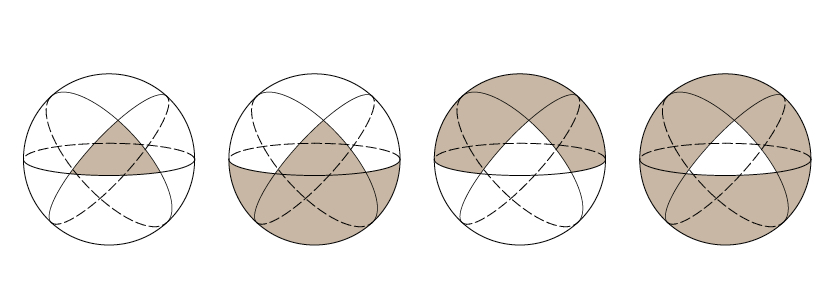
\includegraphics[width=0.9\textwidth]{kugel/Dreieckarten.jpg}
    \captionof{figure}{Dreieckarten auf einer Kugeloberfläche}
\end{center}

Der Begriff Sphärisches Dreieck oder Kugeldreieck ist ein sehr weitläufiger Begriff. 
Dabei können wir den Begriff in drei für uns wesentliche Dreiecke unterteilen:

\begin{itemize}
\item Kugelzweieck
\item Nicht Eulersche’Dreiecke
\item Eulersche’Dreiecke
\end{itemize}

\subsection{Kugelzweieck}

Zwei Grosskreise auf der Kugeloberfläche, zerlegen diese in vier gleiche Kugelzweiecke. 
Jedes dieser Dreieckseiten hat die Länge
$180^{\circ}$ oder $\pi$
Der Flächeninhalt wird dabei nur durch den Winkel $\alpha$ zwischen den beiden Grosskreisen bestimmt.

\begin{center}
        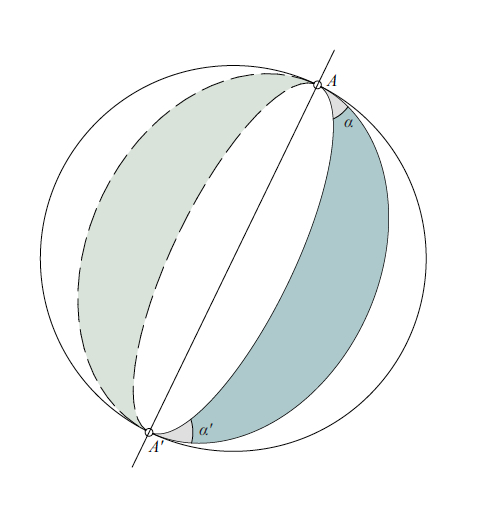
\includegraphics[width=0.3\textwidth]{kugel/Zweieck.jpg}
    \captionof{figure}{Bildung von Zweiecken durch Grosskreise}
\end{center}

Dabei ist der Flächeninhalt der ganzen Kugel:

\begin{align*}
A_{ Kugel } &= 4 \pi r^{2}
\end{align*}


Um den Flächeninhalt des betrachteten Zweieckes zu bekommen, 
müssen wir das ganze noch mit dem Kugelsegment mit dem Winkel $\alpha$ multiplizieren.

\begin{align*}
A_{ Zweieck } &= 4 \pi r^{2} \cdot \frac{ \alpha }{ 2 \pi }
\end{align*}


\subsection{Nicht Eulersche’ Dreiecke}

BLABLA

\subsection{Eulersche’ Dreiecke}

Legt man drei Grosskreise auf eine Kugeloberfläche, bilden sich dabei acht Dreiecke. 
Ein solches Dreieck heisst Eulersches’Dreieck\footnote{%
Leonard Euler (1707-1783), berühmter Schweizer Mathematiker und Physiker. 
Nicht Eulersche’Dreiecke erhält man, indem man das Äussere des Dreieckes ABC betrachtet.} 
Diese Dreiecke werden weder durch die Verlängerung ihrer Seiten durchschnitten, 
noch haben sie Dreiecksseiten welche grösser als $180^{\circ}$ sind.

\begin{center}
        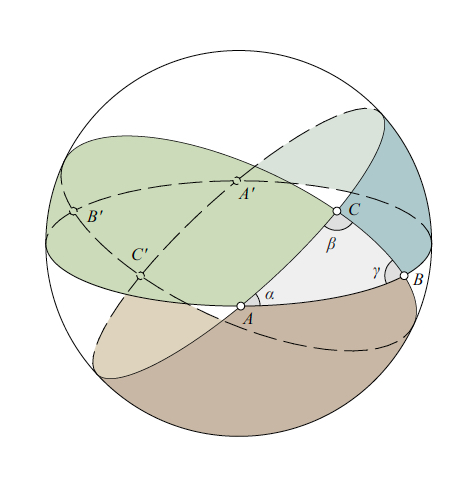
\includegraphics[width=0.4\textwidth]{kugel/Zweiecke.jpg}
    \captionof{figure}{Drei Grosskreise bilden ein sphärisches Dreieck}
\end{center}

In den nachstehenden Erklärungen und Herleitungen, sprechen wir ausschliesslich von Eulerschen’Dreiecken, da die umgeformten Winkelsätze der ebenen Trigonometrie nur auf diese Art von Kugeldreiecken angewendet werden kann.

$A_{ \overline{ ABC }}$ ist die Fläche des Dreieckes auf der Kugeloberfläche
In der ebenen Trigonometrie liegt die Winkelsumme eines Dreiecks bei
$180^{\circ}$.

Anders aber in der sphärischen Trigonometrie. Obschon sie einige Gemeinsamkeiten zur ebenen Trigonometrie aufweist, kann man nicht alles übernehmen.
So auch nicht wie Winkelsumme in einem sphärischen Dreieck.
Diese liegt bei:

\[
\begin{aligned}
\pi
&-
3\pi
&
&\text{\bigg \vert}
&
180^{\circ}
&-
540^{\circ}
\end{aligned}
\]

daraus lässt sich ableiten, das ein einzelner Winkel nicht grösser als $\pi$ oder $180^{\circ}$ sein darf. Ansonsten ist es kein Eulersches’Dreieck und wir dürfen die sphärische Trigonometrie nicht anwenden.\\
Wichtig anzumerken ist, dass die Seiten immer in Radiant beschrieben werden und nicht im Längenmass Meter wie wir es uns gewohnt sind. 
Bei den Dreiecksseiten handelt es sich um Kreisbögen und keine Strecken.

\section{Dreiecksfläche}

\begin{align*}
\text{Zweieck A}
&=
\overline{ABC} + \overline{A'BC} = 2 \alpha r^{ 2 } = A_{ \alpha }\\
\text{Zweieck B}
&=
\overline{ABC} + \overline{AB'C} = 2 \beta r^{ 2 } = A_{ \beta }\\
\text{Zweieck C}
&=
\overline{ABC} + \overline{ABC'} = 2 \gamma r^{ 2 } = A_{ \gamma }
\end{align*}

\begin{align*}
A_{ \alpha } + A_{ \beta } + A_{ \gamma } &= \frac{ 4\pi r^{ 2 } }{ 2 } + 2A_{ \overline{ ABC }} \\
2\alpha r^{ 2 } + 2\beta r^{ 2 } + 2\gamma r^{ 2 } &= \frac{ 4\pi r^{ 2 } }{ 2 } + 2A_{ \overline{ ABC }} \parallel:2\\
\alpha r^{ 2 } + \beta r^{ 2 } + \gamma r^{ 2 } &= \pi r^{ 2 } + A_{ \overline{ ABC }} \parallel-\pi r^{ 2 }\\
r^{ 2 }\left(\alpha + \beta + \gamma - \pi\right) &= A_{ \overline{ ABC }}
\end{align*}




\section{Sphärischer Exzess}
Die Winkelsumme sphärischer Dreiecke ist immer \textgreater \,  $\pi$.

\begin{align*}
\pi < \alpha + \beta + \gamma
\end{align*}

Der sphärische Exzess gibt dabei an, wie stark die Winkelsumme von $\pi$ abweicht.

\begin{align*}
\pi + \epsilon &= \alpha + \beta + \gamma \\
\epsilon &= \alpha + \beta + \gamma - \pi
\end{align*}

Würde der sphärische Exzess in der ebenen Trigonometrie angewendet, wäre dieser = 0. 
Bezieht man das auf die Erde und somit einer Kugel, kann man mit Hilfe eines beliebigen sphärischen Dreieckes und dessen Flächeninhalt auf den Radius der Kugel schliessen.

\subsection{Grenzfall - Satz von Legendre}

\begin{quote} \textit{Ein kleines sphärisches Dreieck kann näherungsweise 
wie ein ebenes Dreieck mit denselben Seiten berechnet 
werden, wenn alle Winkel des ebenen Dreiecks die um 
je ein Drittel des sphärischen Exzesses verminderten 
Winkel des sphärischen Dreiecks nimmt.} \end{quote}
\begin{flushright} - Adrien-Marie Legendre (1752-1833), Paris 1787
\end{flushright}x

Diese Aussage zeigt den Zusammenhang zwischen der 
Trigonometrie in der Ebene sowie in auf der Kugel
auf. Im speziellen bei sehr kleinen sphärischen 
Dreiecken ist die Winkelsumme nur unwesentlich 
grösser als $180^{\circ}$. Des Weiteren kann gesagt werden,
dass der sphärische Exzess gleichmässig auf alle
Winkel aufgeteilt wird.
Wichtig anzumerken ist, dass der Satz von Legendre 
für grosse, aber endliche Radien $r$ gilt.

%[SKIZZE GROSSER RADIUS/KLEINE KRÜMMUNG, KLEINER RADIUS/GROSSE KRÜMMUNG!!!!]
%


\section{Sphärisch Analoge Winkelfunktionen}

\subsection{Sphärischer Sinussatz}

Wir stellen die allgemeinen Sinussätze der Winkel $\alpha$ und $\gamma$ auf:


\[
\begin{aligned}
&{sin(\gamma)} = \frac{h}{a}
&
&\text{\bigg \vert}
&
&{sin(\alpha)} = \frac{h}{c}
&
\end{aligned}
\]

Daraus folgt:
\begin{align*}
h &= sin(\gamma)\cdot a \\
h &= sin(\alpha)\cdot c
\end{align*} 

Durch Gleichsetzung erhält man:
\begin{align*}
h &= h \\
sin(\gamma)\cdot a &= sin(\alpha)\cdot c
\end{align*} 

Durch umstellen erhalten wir den Sinussatz für a und c:
\begin{align*}
sin(\gamma)\cdot a &= sin(\alpha)\cdot c \\
\frac{sin(\gamma)}{c} &= \frac{sin(\alpha)}{a} 
\end{align*} 



\begin{align*}
\frac{sin(\alpha)}{sin(a)} = \frac{sin(\beta)}{sin(b)} = \frac{sin(\gamma)}{sin(c)}
\end{align*} 


\subsection{Winkelkosinussatz}

%[SKIZZE WINKELKOSINUS]

\[
\begin{aligned}
&\overline{C'A'} &= d\cdot {tan(b)}
&
&
&
&
&
&\overline{C'B'} &= d\cdot {tan(a)}
\end{aligned}
\]

\[
\begin{aligned}
&\overline{MA'} &= \frac{ d }{cos(b)}
&
&
&
&
&
&\overline{MB'} &= \frac{ d }{cos(a)}
\end{aligned}
\]

Der allgemeine Kosinussatz beschreibt sich wie folgt:

\begin{align*}
c^{ 2 } &= a^{ 2 } + b^{ 2 } - 2ab \cdot cos(\gamma)
\end{align*}

\begin{align*}
\triangle \overline{A'B'C' }
\overline{ A'B' }^{ 2 } &= \overline{ C'B' }^{ 2 } + \overline{ C'A' }^{ 2 } - 2 \cdot \overline{ C'B' } \cdot \overline{ C'A' } \cdot cos(\gamma)
\end{align*}



\begin{align*}
\overline{A'B'}^{ 2 } &= (d\cdot tan(a))^{ 2 } + (d\cdot tan(b))^{ 2 } - 2 \cdot (d\cdot tan(a) \cdot (d\cdot tan(b) \cdot cos(\gamma)\\
\overline{A'B'}^{ 2 } &= d^{ 2 } \cdot \left(\left(tan^{ 2 }(a) + tan^{ 2 }(b)\right) - 2\cdot tan(a) \cdot tan(b) \cdot cos(\gamma)\right)
\end{align*}

\begin{align*}
\triangle \overline{ MA'B' }
\overline{ A'B' }^{ 2 } &= \overline{ MB' }^{ 2 } + \overline{ MA' }^{ 2 } - 2\cdot \overline{ MB'} \cdot \overline{ MA' } \cdot cos(c)
\end{align*}


\begin{align*}
\overline{ A'B'}^{ 2 } &= \left(\frac{ d }{ cos(a) }  \right)^{ 2 } + \left(\frac{ d }{ cos(b)}  \right)^{ 2 } - 2 \cdot \frac{ d }{ cos(a)} \cdot \frac{ d }{ cos(b)} \cdot cos(c) \\
\overline{ A'B' }^{ 2 } &= d^{ 2 } \cdot \left(\left(\frac{ 1 }{ cos(a) }  \right)^{ 2 } + \left(\frac{ 1 }{ cos(b) }  \right)^{ 2 } - 2 \cdot \frac{ 1 }{ cos(a)} \cdot \frac{ 1 }{ cos(b)} \cdot cos(c)\right)\\
\overline{ A'B' }^{ 2 } &= d^{ 2 } \cdot \left(\left(tan^{ 2 }(a) + 1\right) + \left(tan^{ 2 }(b) + 1\right) - \left(2 \cdot \frac{cos(c)}{cos(a) \cdot cos(b)}\right)\right)
\end{align*}



\begin{align*}
\overline{ A'B'}^{ 2 } &= d^{ 2 } \cdot \left(\left(tan^{ 2 }(a) + tan^{ 2 }(b)\right) - 2 \cdot tan(a) \cdot tan(b) \cdot cos(\gamma)\right) \\
\overline{ A'B'}^{ 2 } &= d^{ 2 } \cdot \left(\left(tan^{ 2 }(a) + 1\right) + \left(tan^{ 2 }(b) + 1\right) - \left(2 \cdot \frac{cos(c)}{cos(a) \cdot cos(b)}\right)\right)
\end{align*}

Die anderen Gleichungen des Satzes, erfolgen aus Symmetriegründen.

\subsection{Seitenkosinussatz}
Durch zyklische Vertauschung des Winkelkosinus erhalten wir den Seitenkosinussatz:

\begin{align*}
{cos(a)} &= {cos(b)} \cdot {cos(c)} + {sin(b)} \cdot {sin(c)} \cdot {sin(\alpha)}\\
{cos(b)} &= {cos(a)} \cdot {cos(c)} + {sin(a)} \cdot {sin(c)} \cdot {sin(\beta)}\\
{cos(c)} &= {cos(a)} \cdot {cos(b)} + {sin(a)} \cdot {sin(b)} \cdot {sin(\gamma)}\\
\end{align*}

\section{Navigation auf See}
Das besondere an Seekarten ist die Inhaltliche Ausrichtung. Anders wie Landkarten muss sie Informationen enthalten welche für den Kapitän und seine Besatzung von grosser Bedeutung sind. Vor allem in Küstennähe ist das navigieren eines Schiffes besonders gefährlich. So enthalten Seekarten etwas über Wassertiefen, Bodenbeschaffenheiten, Gezeiten, Küstenlinien, Landzungen und Windrichtungen.
Der Hauptunterschied dabei ist, das auf der Landkarte feste Positionen definiert und aufgezeigt werden, das einzige was sich verändert ist der Reisende selbst. Bei der Seekarte ist das anders, es werden veränderliche Einwirkungen der Natur festgehalten.

Dieser kleine Unterschied zeigt die Notwendigkeit auf, die Position und den Kurs seines Schiffes auf See immer ermitteln zu können.


\section{Geographische Koordinaten}

Nachdem klar war, das die Erde eine Kugel ist, wurde diese in ein Gradnetz aufgeteilt. Dabei wurden die Angaben für eine exakte Ortsbestimmung klar definiert und die bis heute gültigen Koordinaten bestimmt.
Dabei muss man sich nochmals in Erinnerung rufen, dass sich die Erde in 24h einmal um ihre eigene Achse dreht. Nach $360 ^{\circ}$ 
und somit einer vollen Umdrehung, steht sie wieder in ihrer Ursprungsposition und ein neuer Tag beginnt.

Die Koordinaten setzen sich aus folgenden Komponenten zusammen:

\[
\begin{aligned}
&\text{Grad } (^{\circ})
&
&\text{\bigg \vert}
&
&\text{Bogenminuten } (`)
&
&\text{\bigg \vert}
&
&\text{Bogensekunden } (``)
\end{aligned}
\]

Die Erdoberfläche wurde in je 360 Breiten- und Längengrade eingeteilt. Die Breitengrade haben zueinander einen Abstand von 111.31 km, dies entspricht auch dem Abstand der Längengrade am Äquator mit Zunehmender Nähe zu den Polen, nimmt dieser Abstand ab.

\[
\begin{aligned}
&1^{\circ}
&
&\text{\bigg \vert}
&
&4 \text{ Minuten}
&
&\text{\bigg \vert}
&
&111.31\text{ km}
\end{aligned}
\]

Berechnet man nun die Erdumdrehung von 360°, erhält man genau den Erdumfang am Äquator: \begin{align*} 40’074 \text{ km.}\end{align*}

Dabei geben die Bogenminuten und -sekunden dem Standort die gewünschte Exaktheit. Mit den vollständigen Koordinaten lässt sich der Standort auf einer Landkarte exakt bestimmen und einzeichnen.

\subsection{Zeitzonen der Erde}
Wenn man nun die verschiedenen Zeitzonen der Erde betrachtet, macht die Verschiebung von jeweils einer Stunde durchaus Sinn, es lässt sich auf die Längengrade schliessen.
Zwischen den verschiedenen Zeitzonen liegen 15 Längengrade:

\begin{align*}
\text{15 Längengrade à 4 Minuten = 60 Minuten Zeitverschiebung = ca. 1665 km}
\end{align*}

Dabei ist die Zeitzone in welcher Mitte sich der Greenwich Meredian befindet die \textit{Greenwich Mean Time (GMT)} welche bis 1928 als Weltzeit galt. Im Jahr 1972 wurde diese umbenannt in die \textit{Coordinated Universal Time (UTC)} und wir von da an als Weltzeit $\pm$ 0.00 verwendet.


\section{Der Breitengrad}
Die Breitengrade bilden die bereits genannten Kleinkreise auf der Kugeloberfläche. Sie verlaufen in einem Abstand von genau 111 km parallel zum Äquator. Dabei stellt  dieser genau die Mitte zwischen Nord- und Südpol dar und teilt die Erdkugel in zwei gleiche Hälften. Somit wird von nördlicher und südlicher Breite gesprochen, je nach dem auf welcher Halbkugel man sich befindet.

%[SKIZZE DER GEOGRAFISCHEN BREITE ERDKUGEL]

\subsection{Geografische Breite $\phi$}
\begin{definition}
Die geografische Breite eines Standortes ist nichts anderes, als der Winkel am Erdmittelpunkt zwischen der Ebene des Äquators und der Geraden zum Standpunkt auf der Erdoberfläche.
\end{definition}

%[SKIZZE DER GEOGRAFISCHEN BREITE MIT WINKEL]

\subsection{Navigation mit den Breitengraden}
Da der Breitengrad bereits sehr früh ziemlich präzise bestimmt werden könnte, nutzten bereits die Seefahrer um Christoph Kolumbus den Breitengrad zur Navigation ihrer Flotten.
Den dieser lässt sich ziemlich einfach aus dem höchsten Sonnenstand oder einem Fixstern bestimmen. Dabei wird mit einem Jakobsstab\footnote{%
Der Jakobsstab ist ein früheres astronomisches Instrument zur Winkelmessung und wurde vor allem in der Seefahrt verwendet. Er ist in der Nautik der Vorläufer des Sextanten.} (später Sextant\footnote{%
Der Sextant ist ein nautisches Messinstrument zur Winkelmessung von Horizont und Fixstern (Gestirn)}) der Winkel zwischen dem Horizont und dem Fixstern gemessen. Der Winkel welchen man erhält, zieht man von 90° ab und erhält somit die geografische Breite. \\

%[SKIZZE ERMITTLUNG DES BREITENGRADES]

Wenn man sich auf der Nordhalbkugel befindet, ist der Polarstern ein sehr guter Fixstern. Befindet sich ein Schiff nun sehr nahe am Nordpol, steht dieser nahezu senkrecht am Himmelszelt bei $90^{\circ}$. Würde es aber nahe dem Äquator stehen, erscheint dieser am Horizont bei $0^{\circ}$.

\subsection{Korrekturbeiwert}

\section{Der Längengrad}
Die Längengrade bilden die bereits genannten Grosskreise auf der Kugeloberfläche.
Sie schneiden den Äquator im rechten Winkel, haben dort einen Abstand von 111 km zueinander und verbinden die Pole. Anders wie bei der geografischen Breite, ist in der Natur kein Längengrad gegeben welcher den Nullpunkt darstellt.

%[SKIZZE DER GEOGRAFISCHEN LÄNGE ERDKUGEL]

\subsection{Geografische Länge $\lambda$}
\begin{definition}
Die geografische Länge ist der Winkel an der Erdachse zum Nullmeridian.
\end{definition}

\subsection{Navigation mit den Längengraden}
Die geografische Länge lässt sich nicht so einfach bestimmen wie deren Breite. Für die Berechnung auf See benötigt man eine Referenzzeit eines Ortes mit bekannter Länge.
In der Zeit der Entdecker gab es noch keine mechanischen Uhren. Die Sonnenuhr war zudem ungeeignet, da diese nur die Uhrzeit am Standort mass und nicht die am Referenzort selbst. Die erste Pendeluhr wurde erst Mitte des 17. Jahrhunderts erfunden, was in der Schifffahrt aber auch nicht die Lösung brachte.\\
Pendeluhren auf einem Schiff sind ungeeignet, da das Pendel mit dem Wellengang aus dem Takt gebracht wird und somit die Uhr falsch geht.
Zu ungenau und gegen äussere Erschütterungen zu empfindlich waren später auch die federgetriebenen Uhren und die Unruh. Dazukamen die verschiedenen Klimazonen welche ein Schiff zu durchqueren hatten. Das Metall zog sich viel zu fest zusammen oder dehnte sich aus, was dazu führte das die Uhr unregelmässig lief.

Das sogenannte „Längenproblem“ stellte nicht nur bei der Navigation auf See ein Problem dar, es ergaben sich auch wirtschaftliche Konsequenzen. Die Schiffe mussten bis zur gewünschten geografischen Breite navigieren und segelten dann den Breitengrad entlang. Dabei waren die Schiffe oft Wochenlang unterwegs und segelten die „Breiten ab“ um an die gewünschte Position zu kommen. Dies führte zu erheblichen Zeitverlusten und viel längeren Reisezeiten.


\section{The Board of Longitude - Das Längenproblem}
Das Längenproblem beschäftigte alle grossen Seefahrernationen Europas. Wenn man bedenkt das sich Werte in einer  Höhe von halben britischen Staatshaushalten auf verloren gegangenen Schiffen befanden, erkennt man die Dringlichkeit für eine zuverlässige und genaue Navigation auf See.


\begin{itemize}
\item £ 20’000 - Abweichung von max. einem halben Grad
\item £ 15’000 - Abweichung von zwei Drittel Grad
\item £ 10’000 - Abweichung von max. $1 ^{\circ}$
\end{itemize}

\subsection{John Harrison}


\subsection{Tobias Mayer}



Uhren mit einer Abweichung von einer Minute Abweichung pro Tag (





\section{Nautische Dreieck}


$\Rightarrow$





\section{Die Vermessung der Welt}
Wir schreiben das Jahr 1818 und kehren in die Zeit des Mathematikers Carl Friedrich Gauss zurück. Neben dem liebevoll genannten „kleinen Gauss“ und anderen herausragenden Mathematischen Leistungen, beschäftigte er in den Folgejahren mit der Vermessung des Königreichs Hannovers und verfasste auf 61 Blättern das Kartenwerk \textit{Gauss’sche Landesaufnahme der 1815 durch Hannover erworbenen Gebiete}.






AUFGABE

Hubble Teleskop 
24. April 1990






\printbibliography[heading=subbibliography]
\end{refsection}




%\chapter{Geometrie auf der Kugeloberfläche\label{chapter:kugel}}
\lhead{Geometrie auf der Kugeloberfläche}
\begin{refsection}
\chapterauthor{Melina Staub und Fabian Schmid}

\section{Einleitung}

Schon seit jeher fasziniert den Menschen die Fahrt zur See. Nicht grundlos ist die Seefahrt eine der wichtigsten und ältesten Tätigkeiten der Menschheit. Der innerliche Drang neue Weltmeere und unbekannte Gebiete zu entdecken, die Fahrt zur See zu erleichtern und erträglicher zu machen, trieben die Menschen an, die Schiffe dieser Welt immer weiter zu entwickeln.

Die Idee der Kugelform der Erde ist älter als man zu denken vermag. Bereits der Schüler des antiken griechischen Philosophen Platon - Aristoteles schrieb in seiner Schrift \textit{Über den Himmel} aus dem 4. Jahrhundert v. Chr. etliche Gründe welche für die Gestallt der Erde als Kugel sprechen:

\begin{itemize}
      \item Sämtliche schweren Körper streben zum Mittelpunkt des Alls. Da sie dies von allen Seiten her gleichmäßig tun und die Erde im Mittelpunkt des Alls steht, muss sie eine kugelrunde Gestalt annehmen. 
\item Bei von der Küste wegfahrende Schiffen wird der Rumpf vor den Segeln der Sicht verborgen. 
\item In südlichen Ländern erscheinen südliche Sternbilder höher über dem Horizont.
\item Der Erdschatten bei einer Mondfinsternis ist stets rund.
\end{itemize}

Jedoch war um 1492 - der Zeit der Entdeckung Amerikas durch Christoph Kolumbus, die Idee der Erde in Kugelform noch sehr umstritten. Er erkannte anhand den Theorien und Erkenntnissen der alten Griechen, vor allem Aristoteles, das die Erde eine Kugel sein muss. \\
Doch mit seinem Vorschlag einen Seeweg über den Atlantik nach Indien zu finden und nicht wie üblich um Afrika zu segeln, stiess er beim beim portugiesischen König auf taube Ohren. Sein Plan Indien über eine Route nach Westen zu erreichen, widersprach dem gesunden Menschenverstand. Wäre die Erde wirklich eine Kugel und man befände sich auf der unteren Erdhalbkugel, würde man herunterfallen.\\
Doch auch der damals übliche Glaube an die Erde in Scheibenform brachte so einige Risiken mit sich. Was würde passieren, wenn die Flotte das Ende der Scheibe erreicht hatte? Würden sie über den Erdrand hinweggleiten und in den Abgrund stürzen?\\
Erst nach viel Überzeugungsarbeit durch Kolumbus, setzte er sich am Spanischen Hof durch und segelte über die Westliche Route über den Atlantik und entdeckte schlussendlich Amerika.

Der praktische und greifbare Beweis das die Erde eine Kugel ist, lieferte rund 30 Jahre später der Portugiese Fernando Magellan. Mit seiner Weltumsegelung und seiner Ankunft in den Philippinen, bewies er definitiv das die Erde eine Kugel ist.\\

Nun wollen wir uns die Frage stellen, wie die alten Seefahrer ohne GPS und jeglichen modernen Navigationssystemen auf hoher See wussten wo sie sich befinden und was haben die Sterne mit alldem zu tun? Reisen Sie mit uns zurück in eine Zeit mit Sextant, Kompass und Sternkarten. In die Zeit der Seefahrer und Entdecker.


\section{Geometrie auf der Ebene und der Kugel}

Euklid von Alexandria beschrieb die Grundbegriffe der ebenen Geometrie mittels Punkt, Geraden, Ebene, Winkel und Dreieck. Diese Dreiecke lassen sich mithilfe der ebenen Trigonometrie beschreiben. Dabei gelten die uns bekannten trigonometrischen Winkelfunktionen:\\

\text{Sinussatz:}
\begin{align*}
\frac{ a }{ sin(\alpha) } &= \frac{ b }{sin(\beta)} = \frac{ c }{ sin(\gamma) } = \frac{abc}{2A} = 2r\\
\end{align*}

\text{Cosinussatz:}
\begin{align*}
c^{ 2 } &= a^{ 2 } + b^{ 2 } - 2ab\cdot cos(\gamma)\\
b^{ 2 } &= a^{ 2 } + c^{ 2 } - 2ab\cdot cos(\beta)\\
a^{ 2 } &= b^{ 2 } + c^{ 2 } - 2ab\cdot cos(\alpha)
\end{align*}

Um Dreiecke auf der Kugeloberfläche zu berechnen, benötigt man die sphärische Trigonometrie. Die oben beschriebenen Sätze lassen sich auf der Kugel nicht anwenden, sie werden aber als Grundlage zur Herleitung der Sätze für das Kugeldreieck benötigt.

Die nachfolgenden Seiten thematisieren die Geometrie auf der Kugeloberfläche und wie sie in der Navigation eingesetzt werden kann.


\section{Gross- und Kleinkreise}

Eine Kugeloberfläche lässt sich in zwei verschiedene Kreisarten einteilen -  Gross- und Kleinkreise. 
Wir betrachten als erstes die Grosskreise:

\begin{definition}
Ein Großkreis ist ein größtmöglicher Kreis auf einer Kugeloberfläche. Sein Mittelpunkt fällt immer mit dem Mittelpunkt der Kugel zusammen und ein Schnitt auf dem Großkreis teilt die Kugel in jedem Fall in zwei („gleich große“) Hälften.
\end{definition}

Es gibt unendlich viele Möglichkeiten, eine Kugel in zwei gleich grosse Stücke zu zerschneiden, 
daher gibt es auch unendlich viele Grosskreise. Wenn wir die Grosskreise auf einer Kugel mit diesen auf der Erde beschreiben, sprechen wir von den Längengraden aber auch der Äquator beschreibt einen Grosskreis.
Ein Elementarer Bestandteil bilden die Grosskreise in der sphärischen Trigonometrie. Mithilfe der Schnittpunkte verschiedener Grosskreise, lässt sich ein Sphärisches Dreieck bilden auf welchem sich die sphärische Trigonometrie anwenden lässt.

[GRAFIK GROSSKREISE]

\begin{definition}
Unter Kleinkreis versteht man jene Kreise auf einer Kugeloberfläche, deren Ebenen nicht den Kugelmittelpunkt enthalten.
\end{definition}

Die Kleinkreise eignen sich im Gegensatz zu den Grosskreisen \textit{nicht} für die sphärische Trigonometrie. 
Sie werden lediglich zur Bestimmung der Messgrössen, Winkelabstände oder des Höhenwinkels eines Gestirns verwendet. 

Wenn wir die Kleinkreise auf die Erdoberfläche projizieren betrachten wir die Breitengrade.

[GRAFIK KLEINKREISE]


\section{Sphärische Dreiecke / Kugeldreieck}

\begin{center}
        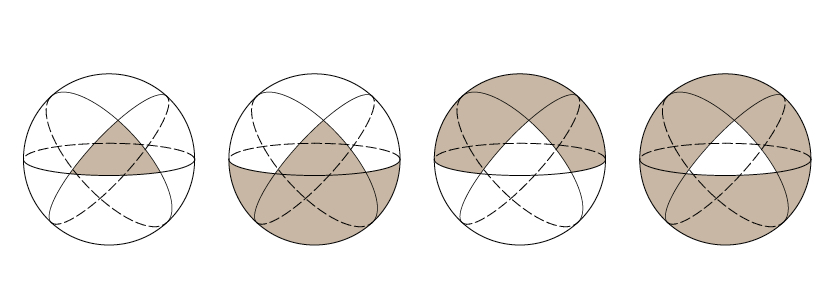
\includegraphics[width=0.9\textwidth]{kugel/Dreieckarten.jpg}
    \captionof{figure}{Dreieckarten auf einer Kugeloberfläche}
\end{center}

Der Begriff Sphärisches Dreieck oder Kugeldreieck ist ein sehr weitläufiger Begriff. 
Dabei können wir den Begriff in drei für uns wesentliche Dreiecke unterteilen:

\begin{itemize}
\item Kugelzweieck
\item Nicht Eulersche’Dreiecke
\item Eulersche’Dreiecke
\end{itemize}

\subsection{Kugelzweieck}

Zwei Grosskreise auf der Kugeloberfläche, zerlegen diese in vier gleiche Kugelzweiecke. 
Jedes dieser Dreieckseiten hat die Länge
$180^{\circ}$ oder $\pi$
Der Flächeninhalt wird dabei nur durch den Winkel $\alpha$ zwischen den beiden Grosskreisen bestimmt.

\begin{center}
        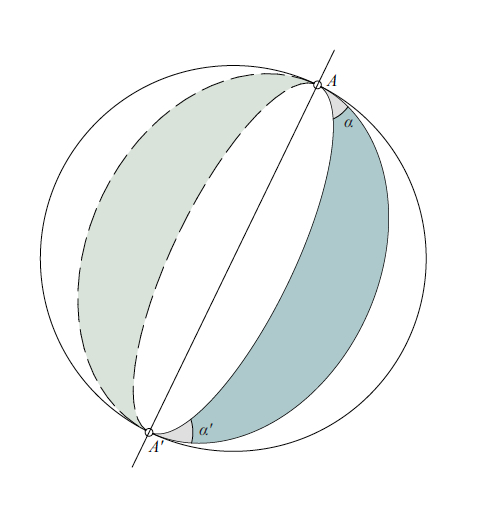
\includegraphics[width=0.3\textwidth]{kugel/Zweieck.jpg}
    \captionof{figure}{Bildung von Zweiecken durch Grosskreise}
\end{center}

Dabei ist der Flächeninhalt der ganzen Kugel:

\begin{align*}
A_{ Kugel } &= 4 \pi r^{2}
\end{align*}


Um den Flächeninhalt des betrachteten Zweieckes zu bekommen, 
müssen wir das ganze noch mit dem Kugelsegment mit dem Winkel $\alpha$ multiplizieren.

\begin{align*}
A_{ Zweieck } &= 4 \pi r^{2} \cdot \frac{ \alpha }{ 2 \pi }
\end{align*}


\subsection{Nicht Eulersche’ Dreiecke}

BLABLA

\subsection{Eulersche’ Dreiecke}

Legt man drei Grosskreise auf eine Kugeloberfläche, bilden sich dabei acht Dreiecke. 
Ein solches Dreieck heisst Eulersches’Dreieck\footnote{%
Leonard Euler (1707-1783), berühmter Schweizer Mathematiker und Physiker. 
Nicht Eulersche’Dreiecke erhält man, indem man das Äussere des Dreieckes ABC betrachtet.} 
Diese Dreiecke werden weder durch die Verlängerung ihrer Seiten durchschnitten, 
noch haben sie Dreiecksseiten welche grösser als $180^{\circ}$ sind.

\begin{center}
        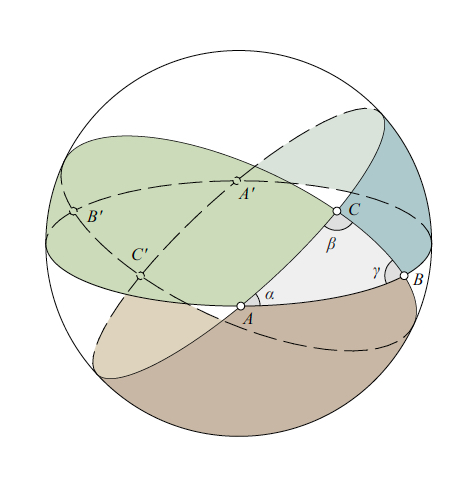
\includegraphics[width=0.4\textwidth]{kugel/Zweiecke.jpg}
    \captionof{figure}{Drei Grosskreise bilden ein sphärisches Dreieck}
\end{center}

In den nachstehenden Erklärungen und Herleitungen, sprechen wir ausschliesslich von Eulerschen’Dreiecken, da die umgeformten Winkelsätze der ebenen Trigonometrie nur auf diese Art von Kugeldreiecken angewendet werden kann.

$A_{ \overline{ ABC }}$ ist die Fläche des Dreieckes auf der Kugeloberfläche
In der ebenen Trigonometrie liegt die Winkelsumme eines Dreiecks bei
$180^{\circ}$.

Anders aber in der sphärischen Trigonometrie. Obschon sie einige Gemeinsamkeiten zur ebenen Trigonometrie aufweist, kann man nicht alles übernehmen.
So auch nicht wie Winkelsumme in einem sphärischen Dreieck.
Diese liegt bei:

\[
\begin{aligned}
\pi
&-
3\pi
&
&\text{\bigg \vert}
&
180^{\circ}
&-
540^{\circ}
\end{aligned}
\]

daraus lässt sich ableiten, das ein einzelner Winkel nicht grösser als $\pi$ oder $180^{\circ}$ sein darf. Ansonsten ist es kein Eulersches’Dreieck und wir dürfen die sphärische Trigonometrie nicht anwenden.\\
Wichtig anzumerken ist, dass die Seiten immer in Radiant beschrieben werden und nicht im Längenmass Meter wie wir es uns gewohnt sind. 
Bei den Dreiecksseiten handelt es sich um Kreisbögen und keine Strecken.

\section{Dreiecksfläche}

\begin{align*}
\text{Zweieck A}
&=
\overline{ABC} + \overline{A'BC} = 2 \alpha r^{ 2 } = A_{ \alpha }\\
\text{Zweieck B}
&=
\overline{ABC} + \overline{AB'C} = 2 \beta r^{ 2 } = A_{ \beta }\\
\text{Zweieck C}
&=
\overline{ABC} + \overline{ABC'} = 2 \gamma r^{ 2 } = A_{ \gamma }
\end{align*}

\begin{align*}
A_{ \alpha } + A_{ \beta } + A_{ \gamma } &= \frac{ 4\pi r^{ 2 } }{ 2 } + 2A_{ \overline{ ABC }} \\
2\alpha r^{ 2 } + 2\beta r^{ 2 } + 2\gamma r^{ 2 } &= \frac{ 4\pi r^{ 2 } }{ 2 } + 2A_{ \overline{ ABC }} \parallel:2\\
\alpha r^{ 2 } + \beta r^{ 2 } + \gamma r^{ 2 } &= \pi r^{ 2 } + A_{ \overline{ ABC }} \parallel-\pi r^{ 2 }\\
r^{ 2 }\left(\alpha + \beta + \gamma - \pi\right) &= A_{ \overline{ ABC }}
\end{align*}




\section{Sphärischer Exzess}
Die Winkelsumme sphärischer Dreiecke ist immer \textgreater \,  $\pi$.

\begin{align*}
\pi < \alpha + \beta + \gamma
\end{align*}

Der sphärische Exzess gibt dabei an, wie stark die Winkelsumme von $\pi$ abweicht.

\begin{align*}
\pi + \epsilon &= \alpha + \beta + \gamma \\
\epsilon &= \alpha + \beta + \gamma - \pi
\end{align*}

Würde der sphärische Exzess in der ebenen Trigonometrie angewendet, wäre dieser = 0. 
Bezieht man das auf die Erde und somit einer Kugel, kann man mit Hilfe eines beliebigen sphärischen Dreieckes und dessen Flächeninhalt auf den Radius der Kugel schliessen.

\subsection{Grenzfall - Satz von Legendre}

\begin{quote} \textit{Ein kleines sphärisches Dreieck kann näherungsweise 
wie ein ebenes Dreieck mit denselben Seiten berechnet 
werden, wenn alle Winkel des ebenen Dreiecks die um 
je ein Drittel des sphärischen Exzesses verminderten 
Winkel des sphärischen Dreiecks nimmt.} \end{quote}
\begin{flushright} - Adrien-Marie Legendre (1752-1833), Paris 1787
\end{flushright}x

Diese Aussage zeigt den Zusammenhang zwischen der 
Trigonometrie in der Ebene sowie in auf der Kugel
auf. Im speziellen bei sehr kleinen sphärischen 
Dreiecken ist die Winkelsumme nur unwesentlich 
grösser als $180^{\circ}$. Des Weiteren kann gesagt werden,
dass der sphärische Exzess gleichmässig auf alle
Winkel aufgeteilt wird.
Wichtig anzumerken ist, dass der Satz von Legendre 
für grosse, aber endliche Radien $r$ gilt.

%[SKIZZE GROSSER RADIUS/KLEINE KRÜMMUNG, KLEINER RADIUS/GROSSE KRÜMMUNG!!!!]
%


\section{Sphärisch Analoge Winkelfunktionen}

\subsection{Sphärischer Sinussatz}

Wir stellen die allgemeinen Sinussätze der Winkel $\alpha$ und $\gamma$ auf:


\[
\begin{aligned}
&{sin(\gamma)} = \frac{h}{a}
&
&\text{\bigg \vert}
&
&{sin(\alpha)} = \frac{h}{c}
&
\end{aligned}
\]

Daraus folgt:
\begin{align*}
h &= sin(\gamma)\cdot a \\
h &= sin(\alpha)\cdot c
\end{align*} 

Durch Gleichsetzung erhält man:
\begin{align*}
h &= h \\
sin(\gamma)\cdot a &= sin(\alpha)\cdot c
\end{align*} 

Durch umstellen erhalten wir den Sinussatz für a und c:
\begin{align*}
sin(\gamma)\cdot a &= sin(\alpha)\cdot c \\
\frac{sin(\gamma)}{c} &= \frac{sin(\alpha)}{a} 
\end{align*} 



\begin{align*}
\frac{sin(\alpha)}{sin(a)} = \frac{sin(\beta)}{sin(b)} = \frac{sin(\gamma)}{sin(c)}
\end{align*} 


\subsection{Winkelkosinussatz}

%[SKIZZE WINKELKOSINUS]

\[
\begin{aligned}
&\overline{C'A'} &= d\cdot {tan(b)}
&
&
&
&
&
&\overline{C'B'} &= d\cdot {tan(a)}
\end{aligned}
\]

\[
\begin{aligned}
&\overline{MA'} &= \frac{ d }{cos(b)}
&
&
&
&
&
&\overline{MB'} &= \frac{ d }{cos(a)}
\end{aligned}
\]

Der allgemeine Kosinussatz beschreibt sich wie folgt:

\begin{align*}
c^{ 2 } &= a^{ 2 } + b^{ 2 } - 2ab \cdot cos(\gamma)
\end{align*}

\begin{align*}
\triangle \overline{A'B'C' }
\overline{ A'B' }^{ 2 } &= \overline{ C'B' }^{ 2 } + \overline{ C'A' }^{ 2 } - 2 \cdot \overline{ C'B' } \cdot \overline{ C'A' } \cdot cos(\gamma)
\end{align*}



\begin{align*}
\overline{A'B'}^{ 2 } &= (d\cdot tan(a))^{ 2 } + (d\cdot tan(b))^{ 2 } - 2 \cdot (d\cdot tan(a) \cdot (d\cdot tan(b) \cdot cos(\gamma)\\
\overline{A'B'}^{ 2 } &= d^{ 2 } \cdot \left(\left(tan^{ 2 }(a) + tan^{ 2 }(b)\right) - 2\cdot tan(a) \cdot tan(b) \cdot cos(\gamma)\right)
\end{align*}

\begin{align*}
\triangle \overline{ MA'B' }
\overline{ A'B' }^{ 2 } &= \overline{ MB' }^{ 2 } + \overline{ MA' }^{ 2 } - 2\cdot \overline{ MB'} \cdot \overline{ MA' } \cdot cos(c)
\end{align*}


\begin{align*}
\overline{ A'B'}^{ 2 } &= \left(\frac{ d }{ cos(a) }  \right)^{ 2 } + \left(\frac{ d }{ cos(b)}  \right)^{ 2 } - 2 \cdot \frac{ d }{ cos(a)} \cdot \frac{ d }{ cos(b)} \cdot cos(c) \\
\overline{ A'B' }^{ 2 } &= d^{ 2 } \cdot \left(\left(\frac{ 1 }{ cos(a) }  \right)^{ 2 } + \left(\frac{ 1 }{ cos(b) }  \right)^{ 2 } - 2 \cdot \frac{ 1 }{ cos(a)} \cdot \frac{ 1 }{ cos(b)} \cdot cos(c)\right)\\
\overline{ A'B' }^{ 2 } &= d^{ 2 } \cdot \left(\left(tan^{ 2 }(a) + 1\right) + \left(tan^{ 2 }(b) + 1\right) - \left(2 \cdot \frac{cos(c)}{cos(a) \cdot cos(b)}\right)\right)
\end{align*}



\begin{align*}
\overline{ A'B'}^{ 2 } &= d^{ 2 } \cdot \left(\left(tan^{ 2 }(a) + tan^{ 2 }(b)\right) - 2 \cdot tan(a) \cdot tan(b) \cdot cos(\gamma)\right) \\
\overline{ A'B'}^{ 2 } &= d^{ 2 } \cdot \left(\left(tan^{ 2 }(a) + 1\right) + \left(tan^{ 2 }(b) + 1\right) - \left(2 \cdot \frac{cos(c)}{cos(a) \cdot cos(b)}\right)\right)
\end{align*}

Die anderen Gleichungen des Satzes, erfolgen aus Symmetriegründen.

\subsection{Seitenkosinussatz}
Durch zyklische Vertauschung des Winkelkosinus erhalten wir den Seitenkosinussatz:

\begin{align*}
{cos(a)} &= {cos(b)} \cdot {cos(c)} + {sin(b)} \cdot {sin(c)} \cdot {sin(\alpha)}\\
{cos(b)} &= {cos(a)} \cdot {cos(c)} + {sin(a)} \cdot {sin(c)} \cdot {sin(\beta)}\\
{cos(c)} &= {cos(a)} \cdot {cos(b)} + {sin(a)} \cdot {sin(b)} \cdot {sin(\gamma)}\\
\end{align*}

\section{Navigation auf See}
Das besondere an Seekarten ist die Inhaltliche Ausrichtung. Anders wie Landkarten muss sie Informationen enthalten welche für den Kapitän und seine Besatzung von grosser Bedeutung sind. Vor allem in Küstennähe ist das navigieren eines Schiffes besonders gefährlich. So enthalten Seekarten etwas über Wassertiefen, Bodenbeschaffenheiten, Gezeiten, Küstenlinien, Landzungen und Windrichtungen.
Der Hauptunterschied dabei ist, das auf der Landkarte feste Positionen definiert und aufgezeigt werden, das einzige was sich verändert ist der Reisende selbst. Bei der Seekarte ist das anders, es werden veränderliche Einwirkungen der Natur festgehalten.

Dieser kleine Unterschied zeigt die Notwendigkeit auf, die Position und den Kurs seines Schiffes auf See immer ermitteln zu können.


\section{Geographische Koordinaten}

Nachdem klar war, das die Erde eine Kugel ist, wurde diese in ein Gradnetz aufgeteilt. Dabei wurden die Angaben für eine exakte Ortsbestimmung klar definiert und die bis heute gültigen Koordinaten bestimmt.
Dabei muss man sich nochmals in Erinnerung rufen, dass sich die Erde in 24h einmal um ihre eigene Achse dreht. Nach $360 ^{\circ}$ 
und somit einer vollen Umdrehung, steht sie wieder in ihrer Ursprungsposition und ein neuer Tag beginnt.

Die Koordinaten setzen sich aus folgenden Komponenten zusammen:

\[
\begin{aligned}
&\text{Grad } (^{\circ})
&
&\text{\bigg \vert}
&
&\text{Bogenminuten } (`)
&
&\text{\bigg \vert}
&
&\text{Bogensekunden } (``)
\end{aligned}
\]

Die Erdoberfläche wurde in je 360 Breiten- und Längengrade eingeteilt. Die Breitengrade haben zueinander einen Abstand von 111.31 km, dies entspricht auch dem Abstand der Längengrade am Äquator mit Zunehmender Nähe zu den Polen, nimmt dieser Abstand ab.

\[
\begin{aligned}
&1^{\circ}
&
&\text{\bigg \vert}
&
&4 \text{ Minuten}
&
&\text{\bigg \vert}
&
&111.31\text{ km}
\end{aligned}
\]

Berechnet man nun die Erdumdrehung von 360°, erhält man genau den Erdumfang am Äquator: \begin{align*} 40’074 \text{ km.}\end{align*}

Dabei geben die Bogenminuten und -sekunden dem Standort die gewünschte Exaktheit. Mit den vollständigen Koordinaten lässt sich der Standort auf einer Landkarte exakt bestimmen und einzeichnen.

\subsection{Zeitzonen der Erde}
Wenn man nun die verschiedenen Zeitzonen der Erde betrachtet, macht die Verschiebung von jeweils einer Stunde durchaus Sinn, es lässt sich auf die Längengrade schliessen.
Zwischen den verschiedenen Zeitzonen liegen 15 Längengrade:

\begin{align*}
\text{15 Längengrade à 4 Minuten = 60 Minuten Zeitverschiebung = ca. 1665 km}
\end{align*}

Dabei ist die Zeitzone in welcher Mitte sich der Greenwich Meredian befindet die \textit{Greenwich Mean Time (GMT)} welche bis 1928 als Weltzeit galt. Im Jahr 1972 wurde diese umbenannt in die \textit{Coordinated Universal Time (UTC)} und wir von da an als Weltzeit $\pm$ 0.00 verwendet.


\section{Der Breitengrad}
Die Breitengrade bilden die bereits genannten Kleinkreise auf der Kugeloberfläche. Sie verlaufen in einem Abstand von genau 111 km parallel zum Äquator. Dabei stellt  dieser genau die Mitte zwischen Nord- und Südpol dar und teilt die Erdkugel in zwei gleiche Hälften. Somit wird von nördlicher und südlicher Breite gesprochen, je nach dem auf welcher Halbkugel man sich befindet.

%[SKIZZE DER GEOGRAFISCHEN BREITE ERDKUGEL]

\subsection{Geografische Breite $\phi$}
\begin{definition}
Die geografische Breite eines Standortes ist nichts anderes, als der Winkel am Erdmittelpunkt zwischen der Ebene des Äquators und der Geraden zum Standpunkt auf der Erdoberfläche.
\end{definition}

%[SKIZZE DER GEOGRAFISCHEN BREITE MIT WINKEL]

\subsection{Navigation mit den Breitengraden}
Da der Breitengrad bereits sehr früh ziemlich präzise bestimmt werden könnte, nutzten bereits die Seefahrer um Christoph Kolumbus den Breitengrad zur Navigation ihrer Flotten.
Den dieser lässt sich ziemlich einfach aus dem höchsten Sonnenstand oder einem Fixstern bestimmen. Dabei wird mit einem Jakobsstab\footnote{%
Der Jakobsstab ist ein früheres astronomisches Instrument zur Winkelmessung und wurde vor allem in der Seefahrt verwendet. Er ist in der Nautik der Vorläufer des Sextanten.} (später Sextant\footnote{%
Der Sextant ist ein nautisches Messinstrument zur Winkelmessung von Horizont und Fixstern (Gestirn)}) der Winkel zwischen dem Horizont und dem Fixstern gemessen. Der Winkel welchen man erhält, zieht man von 90° ab und erhält somit die geografische Breite. \\

%[SKIZZE ERMITTLUNG DES BREITENGRADES]

Wenn man sich auf der Nordhalbkugel befindet, ist der Polarstern ein sehr guter Fixstern. Befindet sich ein Schiff nun sehr nahe am Nordpol, steht dieser nahezu senkrecht am Himmelszelt bei $90^{\circ}$. Würde es aber nahe dem Äquator stehen, erscheint dieser am Horizont bei $0^{\circ}$.

\subsection{Korrekturbeiwert}

\section{Der Längengrad}
Die Längengrade bilden die bereits genannten Grosskreise auf der Kugeloberfläche.
Sie schneiden den Äquator im rechten Winkel, haben dort einen Abstand von 111 km zueinander und verbinden die Pole. Anders wie bei der geografischen Breite, ist in der Natur kein Längengrad gegeben welcher den Nullpunkt darstellt.

%[SKIZZE DER GEOGRAFISCHEN LÄNGE ERDKUGEL]

\subsection{Geografische Länge $\lambda$}
\begin{definition}
Die geografische Länge ist der Winkel an der Erdachse zum Nullmeridian.
\end{definition}

\subsection{Navigation mit den Längengraden}
Die geografische Länge lässt sich nicht so einfach bestimmen wie deren Breite. Für die Berechnung auf See benötigt man eine Referenzzeit eines Ortes mit bekannter Länge.
In der Zeit der Entdecker gab es noch keine mechanischen Uhren. Die Sonnenuhr war zudem ungeeignet, da diese nur die Uhrzeit am Standort mass und nicht die am Referenzort selbst. Die erste Pendeluhr wurde erst Mitte des 17. Jahrhunderts erfunden, was in der Schifffahrt aber auch nicht die Lösung brachte.\\
Pendeluhren auf einem Schiff sind ungeeignet, da das Pendel mit dem Wellengang aus dem Takt gebracht wird und somit die Uhr falsch geht.
Zu ungenau und gegen äussere Erschütterungen zu empfindlich waren später auch die federgetriebenen Uhren und die Unruh. Dazukamen die verschiedenen Klimazonen welche ein Schiff zu durchqueren hatten. Das Metall zog sich viel zu fest zusammen oder dehnte sich aus, was dazu führte das die Uhr unregelmässig lief.

Das sogenannte „Längenproblem“ stellte nicht nur bei der Navigation auf See ein Problem dar, es ergaben sich auch wirtschaftliche Konsequenzen. Die Schiffe mussten bis zur gewünschten geografischen Breite navigieren und segelten dann den Breitengrad entlang. Dabei waren die Schiffe oft Wochenlang unterwegs und segelten die „Breiten ab“ um an die gewünschte Position zu kommen. Dies führte zu erheblichen Zeitverlusten und viel längeren Reisezeiten.


\section{The Board of Longitude - Das Längenproblem}
Das Längenproblem beschäftigte alle grossen Seefahrernationen Europas. Wenn man bedenkt das sich Werte in einer  Höhe von halben britischen Staatshaushalten auf verloren gegangenen Schiffen befanden, erkennt man die Dringlichkeit für eine zuverlässige und genaue Navigation auf See.


\begin{itemize}
\item £ 20’000 - Abweichung von max. einem halben Grad
\item £ 15’000 - Abweichung von zwei Drittel Grad
\item £ 10’000 - Abweichung von max. $1 ^{\circ}$
\end{itemize}

\subsection{John Harrison}


\subsection{Tobias Mayer}



Uhren mit einer Abweichung von einer Minute Abweichung pro Tag (





\section{Nautische Dreieck}


$\Rightarrow$





\section{Die Vermessung der Welt}
Wir schreiben das Jahr 1818 und kehren in die Zeit des Mathematikers Carl Friedrich Gauss zurück. Neben dem liebevoll genannten „kleinen Gauss“ und anderen herausragenden Mathematischen Leistungen, beschäftigte er in den Folgejahren mit der Vermessung des Königreichs Hannovers und verfasste auf 61 Blättern das Kartenwerk \textit{Gauss’sche Landesaufnahme der 1815 durch Hannover erworbenen Gebiete}.






AUFGABE

Hubble Teleskop 
24. April 1990






\printbibliography[heading=subbibliography]
\end{refsection}




%\chapter{Geometrie auf der Kugeloberfläche\label{chapter:kugel}}
\lhead{Geometrie auf der Kugeloberfläche}
\begin{refsection}
\chapterauthor{Melina Staub und Fabian Schmid}

\section{Einleitung}

Schon seit jeher fasziniert den Menschen die Fahrt zur See. Nicht grundlos ist die Seefahrt eine der wichtigsten und ältesten Tätigkeiten der Menschheit. Der innerliche Drang neue Weltmeere und unbekannte Gebiete zu entdecken, die Fahrt zur See zu erleichtern und erträglicher zu machen, trieben die Menschen an, die Schiffe dieser Welt immer weiter zu entwickeln.

Die Idee der Kugelform der Erde ist älter als man zu denken vermag. Bereits der Schüler des antiken griechischen Philosophen Platon - Aristoteles schrieb in seiner Schrift \textit{Über den Himmel} aus dem 4. Jahrhundert v. Chr. etliche Gründe welche für die Gestallt der Erde als Kugel sprechen:

\begin{itemize}
      \item Sämtliche schweren Körper streben zum Mittelpunkt des Alls. Da sie dies von allen Seiten her gleichmäßig tun und die Erde im Mittelpunkt des Alls steht, muss sie eine kugelrunde Gestalt annehmen. 
\item Bei von der Küste wegfahrende Schiffen wird der Rumpf vor den Segeln der Sicht verborgen. 
\item In südlichen Ländern erscheinen südliche Sternbilder höher über dem Horizont.
\item Der Erdschatten bei einer Mondfinsternis ist stets rund.
\end{itemize}

Jedoch war um 1492 - der Zeit der Entdeckung Amerikas durch Christoph Kolumbus, die Idee der Erde in Kugelform noch sehr umstritten. Er erkannte anhand den Theorien und Erkenntnissen der alten Griechen, vor allem Aristoteles, das die Erde eine Kugel sein muss. \\
Doch mit seinem Vorschlag einen Seeweg über den Atlantik nach Indien zu finden und nicht wie üblich um Afrika zu segeln, stiess er beim beim portugiesischen König auf taube Ohren. Sein Plan Indien über eine Route nach Westen zu erreichen, widersprach dem gesunden Menschenverstand. Wäre die Erde wirklich eine Kugel und man befände sich auf der unteren Erdhalbkugel, würde man herunterfallen.\\
Doch auch der damals übliche Glaube an die Erde in Scheibenform brachte so einige Risiken mit sich. Was würde passieren, wenn die Flotte das Ende der Scheibe erreicht hatte? Würden sie über den Erdrand hinweggleiten und in den Abgrund stürzen?\\
Erst nach viel Überzeugungsarbeit durch Kolumbus, setzte er sich am Spanischen Hof durch und segelte über die Westliche Route über den Atlantik und entdeckte schlussendlich Amerika.

Der praktische und greifbare Beweis das die Erde eine Kugel ist, lieferte rund 30 Jahre später der Portugiese Fernando Magellan. Mit seiner Weltumsegelung und seiner Ankunft in den Philippinen, bewies er definitiv das die Erde eine Kugel ist.\\

Nun wollen wir uns die Frage stellen, wie die alten Seefahrer ohne GPS und jeglichen modernen Navigationssystemen auf hoher See wussten wo sie sich befinden und was haben die Sterne mit alldem zu tun? Reisen Sie mit uns zurück in eine Zeit mit Sextant, Kompass und Sternkarten. In die Zeit der Seefahrer und Entdecker.


\section{Geometrie auf der Ebene und der Kugel}

Euklid von Alexandria beschrieb die Grundbegriffe der ebenen Geometrie mittels Punkt, Geraden, Ebene, Winkel und Dreieck. Diese Dreiecke lassen sich mithilfe der ebenen Trigonometrie beschreiben. Dabei gelten die uns bekannten trigonometrischen Winkelfunktionen:\\

\text{Sinussatz:}
\begin{align*}
\frac{ a }{ sin(\alpha) } &= \frac{ b }{sin(\beta)} = \frac{ c }{ sin(\gamma) } = \frac{abc}{2A} = 2r\\
\end{align*}

\text{Cosinussatz:}
\begin{align*}
c^{ 2 } &= a^{ 2 } + b^{ 2 } - 2ab\cdot cos(\gamma)\\
b^{ 2 } &= a^{ 2 } + c^{ 2 } - 2ab\cdot cos(\beta)\\
a^{ 2 } &= b^{ 2 } + c^{ 2 } - 2ab\cdot cos(\alpha)
\end{align*}

Um Dreiecke auf der Kugeloberfläche zu berechnen, benötigt man die sphärische Trigonometrie. Die oben beschriebenen Sätze lassen sich auf der Kugel nicht anwenden, sie werden aber als Grundlage zur Herleitung der Sätze für das Kugeldreieck benötigt.

Die nachfolgenden Seiten thematisieren die Geometrie auf der Kugeloberfläche und wie sie in der Navigation eingesetzt werden kann.


\section{Gross- und Kleinkreise}

Eine Kugeloberfläche lässt sich in zwei verschiedene Kreisarten einteilen -  Gross- und Kleinkreise. 
Wir betrachten als erstes die Grosskreise:

\begin{definition}
Ein Großkreis ist ein größtmöglicher Kreis auf einer Kugeloberfläche. Sein Mittelpunkt fällt immer mit dem Mittelpunkt der Kugel zusammen und ein Schnitt auf dem Großkreis teilt die Kugel in jedem Fall in zwei („gleich große“) Hälften.
\end{definition}

Es gibt unendlich viele Möglichkeiten, eine Kugel in zwei gleich grosse Stücke zu zerschneiden, 
daher gibt es auch unendlich viele Grosskreise. Wenn wir die Grosskreise auf einer Kugel mit diesen auf der Erde beschreiben, sprechen wir von den Längengraden aber auch der Äquator beschreibt einen Grosskreis.
Ein Elementarer Bestandteil bilden die Grosskreise in der sphärischen Trigonometrie. Mithilfe der Schnittpunkte verschiedener Grosskreise, lässt sich ein Sphärisches Dreieck bilden auf welchem sich die sphärische Trigonometrie anwenden lässt.

[GRAFIK GROSSKREISE]

\begin{definition}
Unter Kleinkreis versteht man jene Kreise auf einer Kugeloberfläche, deren Ebenen nicht den Kugelmittelpunkt enthalten.
\end{definition}

Die Kleinkreise eignen sich im Gegensatz zu den Grosskreisen \textit{nicht} für die sphärische Trigonometrie. 
Sie werden lediglich zur Bestimmung der Messgrössen, Winkelabstände oder des Höhenwinkels eines Gestirns verwendet. 

Wenn wir die Kleinkreise auf die Erdoberfläche projizieren betrachten wir die Breitengrade.

[GRAFIK KLEINKREISE]


\section{Sphärische Dreiecke / Kugeldreieck}

\begin{center}
        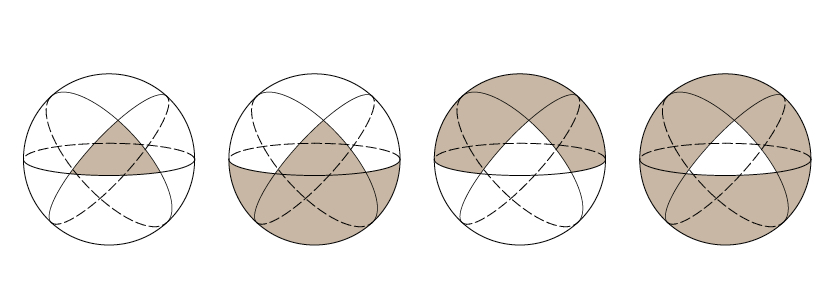
\includegraphics[width=0.9\textwidth]{kugel/Dreieckarten.jpg}
    \captionof{figure}{Dreieckarten auf einer Kugeloberfläche}
\end{center}

Der Begriff Sphärisches Dreieck oder Kugeldreieck ist ein sehr weitläufiger Begriff. 
Dabei können wir den Begriff in drei für uns wesentliche Dreiecke unterteilen:

\begin{itemize}
\item Kugelzweieck
\item Nicht Eulersche’Dreiecke
\item Eulersche’Dreiecke
\end{itemize}

\subsection{Kugelzweieck}

Zwei Grosskreise auf der Kugeloberfläche, zerlegen diese in vier gleiche Kugelzweiecke. 
Jedes dieser Dreieckseiten hat die Länge
$180^{\circ}$ oder $\pi$
Der Flächeninhalt wird dabei nur durch den Winkel $\alpha$ zwischen den beiden Grosskreisen bestimmt.

\begin{center}
        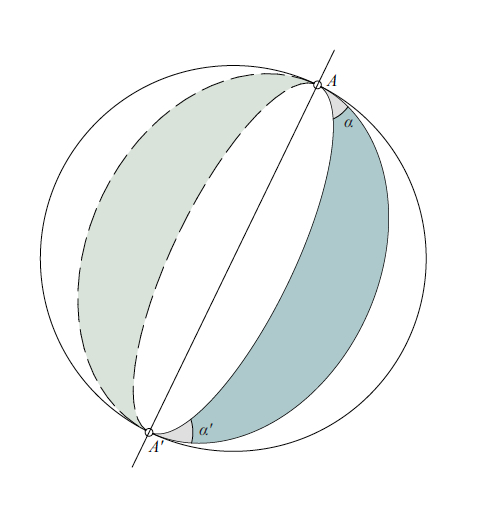
\includegraphics[width=0.3\textwidth]{kugel/Zweieck.jpg}
    \captionof{figure}{Bildung von Zweiecken durch Grosskreise}
\end{center}

Dabei ist der Flächeninhalt der ganzen Kugel:

\begin{align*}
A_{ Kugel } &= 4 \pi r^{2}
\end{align*}


Um den Flächeninhalt des betrachteten Zweieckes zu bekommen, 
müssen wir das ganze noch mit dem Kugelsegment mit dem Winkel $\alpha$ multiplizieren.

\begin{align*}
A_{ Zweieck } &= 4 \pi r^{2} \cdot \frac{ \alpha }{ 2 \pi }
\end{align*}


\subsection{Nicht Eulersche’ Dreiecke}

BLABLA

\subsection{Eulersche’ Dreiecke}

Legt man drei Grosskreise auf eine Kugeloberfläche, bilden sich dabei acht Dreiecke. 
Ein solches Dreieck heisst Eulersches’Dreieck\footnote{%
Leonard Euler (1707-1783), berühmter Schweizer Mathematiker und Physiker. 
Nicht Eulersche’Dreiecke erhält man, indem man das Äussere des Dreieckes ABC betrachtet.} 
Diese Dreiecke werden weder durch die Verlängerung ihrer Seiten durchschnitten, 
noch haben sie Dreiecksseiten welche grösser als $180^{\circ}$ sind.

\begin{center}
        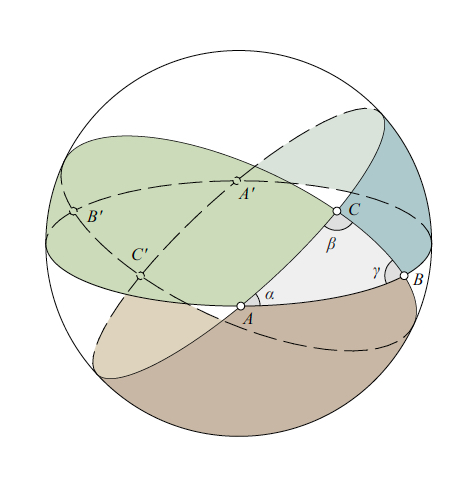
\includegraphics[width=0.4\textwidth]{kugel/Zweiecke.jpg}
    \captionof{figure}{Drei Grosskreise bilden ein sphärisches Dreieck}
\end{center}

In den nachstehenden Erklärungen und Herleitungen, sprechen wir ausschliesslich von Eulerschen’Dreiecken, da die umgeformten Winkelsätze der ebenen Trigonometrie nur auf diese Art von Kugeldreiecken angewendet werden kann.

$A_{ \overline{ ABC }}$ ist die Fläche des Dreieckes auf der Kugeloberfläche
In der ebenen Trigonometrie liegt die Winkelsumme eines Dreiecks bei
$180^{\circ}$.

Anders aber in der sphärischen Trigonometrie. Obschon sie einige Gemeinsamkeiten zur ebenen Trigonometrie aufweist, kann man nicht alles übernehmen.
So auch nicht wie Winkelsumme in einem sphärischen Dreieck.
Diese liegt bei:

\[
\begin{aligned}
\pi
&-
3\pi
&
&\text{\bigg \vert}
&
180^{\circ}
&-
540^{\circ}
\end{aligned}
\]

daraus lässt sich ableiten, das ein einzelner Winkel nicht grösser als $\pi$ oder $180^{\circ}$ sein darf. Ansonsten ist es kein Eulersches’Dreieck und wir dürfen die sphärische Trigonometrie nicht anwenden.\\
Wichtig anzumerken ist, dass die Seiten immer in Radiant beschrieben werden und nicht im Längenmass Meter wie wir es uns gewohnt sind. 
Bei den Dreiecksseiten handelt es sich um Kreisbögen und keine Strecken.

\section{Dreiecksfläche}

\begin{align*}
\text{Zweieck A}
&=
\overline{ABC} + \overline{A'BC} = 2 \alpha r^{ 2 } = A_{ \alpha }\\
\text{Zweieck B}
&=
\overline{ABC} + \overline{AB'C} = 2 \beta r^{ 2 } = A_{ \beta }\\
\text{Zweieck C}
&=
\overline{ABC} + \overline{ABC'} = 2 \gamma r^{ 2 } = A_{ \gamma }
\end{align*}

\begin{align*}
A_{ \alpha } + A_{ \beta } + A_{ \gamma } &= \frac{ 4\pi r^{ 2 } }{ 2 } + 2A_{ \overline{ ABC }} \\
2\alpha r^{ 2 } + 2\beta r^{ 2 } + 2\gamma r^{ 2 } &= \frac{ 4\pi r^{ 2 } }{ 2 } + 2A_{ \overline{ ABC }} \parallel:2\\
\alpha r^{ 2 } + \beta r^{ 2 } + \gamma r^{ 2 } &= \pi r^{ 2 } + A_{ \overline{ ABC }} \parallel-\pi r^{ 2 }\\
r^{ 2 }\left(\alpha + \beta + \gamma - \pi\right) &= A_{ \overline{ ABC }}
\end{align*}




\section{Sphärischer Exzess}
Die Winkelsumme sphärischer Dreiecke ist immer \textgreater \,  $\pi$.

\begin{align*}
\pi < \alpha + \beta + \gamma
\end{align*}

Der sphärische Exzess gibt dabei an, wie stark die Winkelsumme von $\pi$ abweicht.

\begin{align*}
\pi + \epsilon &= \alpha + \beta + \gamma \\
\epsilon &= \alpha + \beta + \gamma - \pi
\end{align*}

Würde der sphärische Exzess in der ebenen Trigonometrie angewendet, wäre dieser = 0. 
Bezieht man das auf die Erde und somit einer Kugel, kann man mit Hilfe eines beliebigen sphärischen Dreieckes und dessen Flächeninhalt auf den Radius der Kugel schliessen.

\subsection{Grenzfall - Satz von Legendre}

\begin{quote} \textit{Ein kleines sphärisches Dreieck kann näherungsweise 
wie ein ebenes Dreieck mit denselben Seiten berechnet 
werden, wenn alle Winkel des ebenen Dreiecks die um 
je ein Drittel des sphärischen Exzesses verminderten 
Winkel des sphärischen Dreiecks nimmt.} \end{quote}
\begin{flushright} - Adrien-Marie Legendre (1752-1833), Paris 1787
\end{flushright}x

Diese Aussage zeigt den Zusammenhang zwischen der 
Trigonometrie in der Ebene sowie in auf der Kugel
auf. Im speziellen bei sehr kleinen sphärischen 
Dreiecken ist die Winkelsumme nur unwesentlich 
grösser als $180^{\circ}$. Des Weiteren kann gesagt werden,
dass der sphärische Exzess gleichmässig auf alle
Winkel aufgeteilt wird.
Wichtig anzumerken ist, dass der Satz von Legendre 
für grosse, aber endliche Radien $r$ gilt.

%[SKIZZE GROSSER RADIUS/KLEINE KRÜMMUNG, KLEINER RADIUS/GROSSE KRÜMMUNG!!!!]
%


\section{Sphärisch Analoge Winkelfunktionen}

\subsection{Sphärischer Sinussatz}

Wir stellen die allgemeinen Sinussätze der Winkel $\alpha$ und $\gamma$ auf:


\[
\begin{aligned}
&{sin(\gamma)} = \frac{h}{a}
&
&\text{\bigg \vert}
&
&{sin(\alpha)} = \frac{h}{c}
&
\end{aligned}
\]

Daraus folgt:
\begin{align*}
h &= sin(\gamma)\cdot a \\
h &= sin(\alpha)\cdot c
\end{align*} 

Durch Gleichsetzung erhält man:
\begin{align*}
h &= h \\
sin(\gamma)\cdot a &= sin(\alpha)\cdot c
\end{align*} 

Durch umstellen erhalten wir den Sinussatz für a und c:
\begin{align*}
sin(\gamma)\cdot a &= sin(\alpha)\cdot c \\
\frac{sin(\gamma)}{c} &= \frac{sin(\alpha)}{a} 
\end{align*} 



\begin{align*}
\frac{sin(\alpha)}{sin(a)} = \frac{sin(\beta)}{sin(b)} = \frac{sin(\gamma)}{sin(c)}
\end{align*} 


\subsection{Winkelkosinussatz}

%[SKIZZE WINKELKOSINUS]

\[
\begin{aligned}
&\overline{C'A'} &= d\cdot {tan(b)}
&
&
&
&
&
&\overline{C'B'} &= d\cdot {tan(a)}
\end{aligned}
\]

\[
\begin{aligned}
&\overline{MA'} &= \frac{ d }{cos(b)}
&
&
&
&
&
&\overline{MB'} &= \frac{ d }{cos(a)}
\end{aligned}
\]

Der allgemeine Kosinussatz beschreibt sich wie folgt:

\begin{align*}
c^{ 2 } &= a^{ 2 } + b^{ 2 } - 2ab \cdot cos(\gamma)
\end{align*}

\begin{align*}
\triangle \overline{A'B'C' }
\overline{ A'B' }^{ 2 } &= \overline{ C'B' }^{ 2 } + \overline{ C'A' }^{ 2 } - 2 \cdot \overline{ C'B' } \cdot \overline{ C'A' } \cdot cos(\gamma)
\end{align*}



\begin{align*}
\overline{A'B'}^{ 2 } &= (d\cdot tan(a))^{ 2 } + (d\cdot tan(b))^{ 2 } - 2 \cdot (d\cdot tan(a) \cdot (d\cdot tan(b) \cdot cos(\gamma)\\
\overline{A'B'}^{ 2 } &= d^{ 2 } \cdot \left(\left(tan^{ 2 }(a) + tan^{ 2 }(b)\right) - 2\cdot tan(a) \cdot tan(b) \cdot cos(\gamma)\right)
\end{align*}

\begin{align*}
\triangle \overline{ MA'B' }
\overline{ A'B' }^{ 2 } &= \overline{ MB' }^{ 2 } + \overline{ MA' }^{ 2 } - 2\cdot \overline{ MB'} \cdot \overline{ MA' } \cdot cos(c)
\end{align*}


\begin{align*}
\overline{ A'B'}^{ 2 } &= \left(\frac{ d }{ cos(a) }  \right)^{ 2 } + \left(\frac{ d }{ cos(b)}  \right)^{ 2 } - 2 \cdot \frac{ d }{ cos(a)} \cdot \frac{ d }{ cos(b)} \cdot cos(c) \\
\overline{ A'B' }^{ 2 } &= d^{ 2 } \cdot \left(\left(\frac{ 1 }{ cos(a) }  \right)^{ 2 } + \left(\frac{ 1 }{ cos(b) }  \right)^{ 2 } - 2 \cdot \frac{ 1 }{ cos(a)} \cdot \frac{ 1 }{ cos(b)} \cdot cos(c)\right)\\
\overline{ A'B' }^{ 2 } &= d^{ 2 } \cdot \left(\left(tan^{ 2 }(a) + 1\right) + \left(tan^{ 2 }(b) + 1\right) - \left(2 \cdot \frac{cos(c)}{cos(a) \cdot cos(b)}\right)\right)
\end{align*}



\begin{align*}
\overline{ A'B'}^{ 2 } &= d^{ 2 } \cdot \left(\left(tan^{ 2 }(a) + tan^{ 2 }(b)\right) - 2 \cdot tan(a) \cdot tan(b) \cdot cos(\gamma)\right) \\
\overline{ A'B'}^{ 2 } &= d^{ 2 } \cdot \left(\left(tan^{ 2 }(a) + 1\right) + \left(tan^{ 2 }(b) + 1\right) - \left(2 \cdot \frac{cos(c)}{cos(a) \cdot cos(b)}\right)\right)
\end{align*}

Die anderen Gleichungen des Satzes, erfolgen aus Symmetriegründen.

\subsection{Seitenkosinussatz}
Durch zyklische Vertauschung des Winkelkosinus erhalten wir den Seitenkosinussatz:

\begin{align*}
{cos(a)} &= {cos(b)} \cdot {cos(c)} + {sin(b)} \cdot {sin(c)} \cdot {sin(\alpha)}\\
{cos(b)} &= {cos(a)} \cdot {cos(c)} + {sin(a)} \cdot {sin(c)} \cdot {sin(\beta)}\\
{cos(c)} &= {cos(a)} \cdot {cos(b)} + {sin(a)} \cdot {sin(b)} \cdot {sin(\gamma)}\\
\end{align*}

\section{Navigation auf See}
Das besondere an Seekarten ist die Inhaltliche Ausrichtung. Anders wie Landkarten muss sie Informationen enthalten welche für den Kapitän und seine Besatzung von grosser Bedeutung sind. Vor allem in Küstennähe ist das navigieren eines Schiffes besonders gefährlich. So enthalten Seekarten etwas über Wassertiefen, Bodenbeschaffenheiten, Gezeiten, Küstenlinien, Landzungen und Windrichtungen.
Der Hauptunterschied dabei ist, das auf der Landkarte feste Positionen definiert und aufgezeigt werden, das einzige was sich verändert ist der Reisende selbst. Bei der Seekarte ist das anders, es werden veränderliche Einwirkungen der Natur festgehalten.

Dieser kleine Unterschied zeigt die Notwendigkeit auf, die Position und den Kurs seines Schiffes auf See immer ermitteln zu können.


\section{Geographische Koordinaten}

Nachdem klar war, das die Erde eine Kugel ist, wurde diese in ein Gradnetz aufgeteilt. Dabei wurden die Angaben für eine exakte Ortsbestimmung klar definiert und die bis heute gültigen Koordinaten bestimmt.
Dabei muss man sich nochmals in Erinnerung rufen, dass sich die Erde in 24h einmal um ihre eigene Achse dreht. Nach $360 ^{\circ}$ 
und somit einer vollen Umdrehung, steht sie wieder in ihrer Ursprungsposition und ein neuer Tag beginnt.

Die Koordinaten setzen sich aus folgenden Komponenten zusammen:

\[
\begin{aligned}
&\text{Grad } (^{\circ})
&
&\text{\bigg \vert}
&
&\text{Bogenminuten } (`)
&
&\text{\bigg \vert}
&
&\text{Bogensekunden } (``)
\end{aligned}
\]

Die Erdoberfläche wurde in je 360 Breiten- und Längengrade eingeteilt. Die Breitengrade haben zueinander einen Abstand von 111.31 km, dies entspricht auch dem Abstand der Längengrade am Äquator mit Zunehmender Nähe zu den Polen, nimmt dieser Abstand ab.

\[
\begin{aligned}
&1^{\circ}
&
&\text{\bigg \vert}
&
&4 \text{ Minuten}
&
&\text{\bigg \vert}
&
&111.31\text{ km}
\end{aligned}
\]

Berechnet man nun die Erdumdrehung von 360°, erhält man genau den Erdumfang am Äquator: \begin{align*} 40’074 \text{ km.}\end{align*}

Dabei geben die Bogenminuten und -sekunden dem Standort die gewünschte Exaktheit. Mit den vollständigen Koordinaten lässt sich der Standort auf einer Landkarte exakt bestimmen und einzeichnen.

\subsection{Zeitzonen der Erde}
Wenn man nun die verschiedenen Zeitzonen der Erde betrachtet, macht die Verschiebung von jeweils einer Stunde durchaus Sinn, es lässt sich auf die Längengrade schliessen.
Zwischen den verschiedenen Zeitzonen liegen 15 Längengrade:

\begin{align*}
\text{15 Längengrade à 4 Minuten = 60 Minuten Zeitverschiebung = ca. 1665 km}
\end{align*}

Dabei ist die Zeitzone in welcher Mitte sich der Greenwich Meredian befindet die \textit{Greenwich Mean Time (GMT)} welche bis 1928 als Weltzeit galt. Im Jahr 1972 wurde diese umbenannt in die \textit{Coordinated Universal Time (UTC)} und wir von da an als Weltzeit $\pm$ 0.00 verwendet.


\section{Der Breitengrad}
Die Breitengrade bilden die bereits genannten Kleinkreise auf der Kugeloberfläche. Sie verlaufen in einem Abstand von genau 111 km parallel zum Äquator. Dabei stellt  dieser genau die Mitte zwischen Nord- und Südpol dar und teilt die Erdkugel in zwei gleiche Hälften. Somit wird von nördlicher und südlicher Breite gesprochen, je nach dem auf welcher Halbkugel man sich befindet.

%[SKIZZE DER GEOGRAFISCHEN BREITE ERDKUGEL]

\subsection{Geografische Breite $\phi$}
\begin{definition}
Die geografische Breite eines Standortes ist nichts anderes, als der Winkel am Erdmittelpunkt zwischen der Ebene des Äquators und der Geraden zum Standpunkt auf der Erdoberfläche.
\end{definition}

%[SKIZZE DER GEOGRAFISCHEN BREITE MIT WINKEL]

\subsection{Navigation mit den Breitengraden}
Da der Breitengrad bereits sehr früh ziemlich präzise bestimmt werden könnte, nutzten bereits die Seefahrer um Christoph Kolumbus den Breitengrad zur Navigation ihrer Flotten.
Den dieser lässt sich ziemlich einfach aus dem höchsten Sonnenstand oder einem Fixstern bestimmen. Dabei wird mit einem Jakobsstab\footnote{%
Der Jakobsstab ist ein früheres astronomisches Instrument zur Winkelmessung und wurde vor allem in der Seefahrt verwendet. Er ist in der Nautik der Vorläufer des Sextanten.} (später Sextant\footnote{%
Der Sextant ist ein nautisches Messinstrument zur Winkelmessung von Horizont und Fixstern (Gestirn)}) der Winkel zwischen dem Horizont und dem Fixstern gemessen. Der Winkel welchen man erhält, zieht man von 90° ab und erhält somit die geografische Breite. \\

%[SKIZZE ERMITTLUNG DES BREITENGRADES]

Wenn man sich auf der Nordhalbkugel befindet, ist der Polarstern ein sehr guter Fixstern. Befindet sich ein Schiff nun sehr nahe am Nordpol, steht dieser nahezu senkrecht am Himmelszelt bei $90^{\circ}$. Würde es aber nahe dem Äquator stehen, erscheint dieser am Horizont bei $0^{\circ}$.

\subsection{Korrekturbeiwert}

\section{Der Längengrad}
Die Längengrade bilden die bereits genannten Grosskreise auf der Kugeloberfläche.
Sie schneiden den Äquator im rechten Winkel, haben dort einen Abstand von 111 km zueinander und verbinden die Pole. Anders wie bei der geografischen Breite, ist in der Natur kein Längengrad gegeben welcher den Nullpunkt darstellt.

%[SKIZZE DER GEOGRAFISCHEN LÄNGE ERDKUGEL]

\subsection{Geografische Länge $\lambda$}
\begin{definition}
Die geografische Länge ist der Winkel an der Erdachse zum Nullmeridian.
\end{definition}

\subsection{Navigation mit den Längengraden}
Die geografische Länge lässt sich nicht so einfach bestimmen wie deren Breite. Für die Berechnung auf See benötigt man eine Referenzzeit eines Ortes mit bekannter Länge.
In der Zeit der Entdecker gab es noch keine mechanischen Uhren. Die Sonnenuhr war zudem ungeeignet, da diese nur die Uhrzeit am Standort mass und nicht die am Referenzort selbst. Die erste Pendeluhr wurde erst Mitte des 17. Jahrhunderts erfunden, was in der Schifffahrt aber auch nicht die Lösung brachte.\\
Pendeluhren auf einem Schiff sind ungeeignet, da das Pendel mit dem Wellengang aus dem Takt gebracht wird und somit die Uhr falsch geht.
Zu ungenau und gegen äussere Erschütterungen zu empfindlich waren später auch die federgetriebenen Uhren und die Unruh. Dazukamen die verschiedenen Klimazonen welche ein Schiff zu durchqueren hatten. Das Metall zog sich viel zu fest zusammen oder dehnte sich aus, was dazu führte das die Uhr unregelmässig lief.

Das sogenannte „Längenproblem“ stellte nicht nur bei der Navigation auf See ein Problem dar, es ergaben sich auch wirtschaftliche Konsequenzen. Die Schiffe mussten bis zur gewünschten geografischen Breite navigieren und segelten dann den Breitengrad entlang. Dabei waren die Schiffe oft Wochenlang unterwegs und segelten die „Breiten ab“ um an die gewünschte Position zu kommen. Dies führte zu erheblichen Zeitverlusten und viel längeren Reisezeiten.


\section{The Board of Longitude - Das Längenproblem}
Das Längenproblem beschäftigte alle grossen Seefahrernationen Europas. Wenn man bedenkt das sich Werte in einer  Höhe von halben britischen Staatshaushalten auf verloren gegangenen Schiffen befanden, erkennt man die Dringlichkeit für eine zuverlässige und genaue Navigation auf See.


\begin{itemize}
\item £ 20’000 - Abweichung von max. einem halben Grad
\item £ 15’000 - Abweichung von zwei Drittel Grad
\item £ 10’000 - Abweichung von max. $1 ^{\circ}$
\end{itemize}

\subsection{John Harrison}


\subsection{Tobias Mayer}



Uhren mit einer Abweichung von einer Minute Abweichung pro Tag (





\section{Nautische Dreieck}


$\Rightarrow$





\section{Die Vermessung der Welt}
Wir schreiben das Jahr 1818 und kehren in die Zeit des Mathematikers Carl Friedrich Gauss zurück. Neben dem liebevoll genannten „kleinen Gauss“ und anderen herausragenden Mathematischen Leistungen, beschäftigte er in den Folgejahren mit der Vermessung des Königreichs Hannovers und verfasste auf 61 Blättern das Kartenwerk \textit{Gauss’sche Landesaufnahme der 1815 durch Hannover erworbenen Gebiete}.






AUFGABE

Hubble Teleskop 
24. April 1990






\printbibliography[heading=subbibliography]
\end{refsection}




%\chapter{Geometrie auf der Kugeloberfläche\label{chapter:kugel}}
\lhead{Geometrie auf der Kugeloberfläche}
\begin{refsection}
\chapterauthor{Melina Staub und Fabian Schmid}

\section{Einleitung}

Schon seit jeher fasziniert den Menschen die Fahrt zur See. Nicht grundlos ist die Seefahrt eine der wichtigsten und ältesten Tätigkeiten der Menschheit. Der innerliche Drang neue Weltmeere und unbekannte Gebiete zu entdecken, die Fahrt zur See zu erleichtern und erträglicher zu machen, trieben die Menschen an, die Schiffe dieser Welt immer weiter zu entwickeln.

Die Idee der Kugelform der Erde ist älter als man zu denken vermag. Bereits der Schüler des antiken griechischen Philosophen Platon - Aristoteles schrieb in seiner Schrift \textit{Über den Himmel} aus dem 4. Jahrhundert v. Chr. etliche Gründe welche für die Gestallt der Erde als Kugel sprechen:

\begin{itemize}
      \item Sämtliche schweren Körper streben zum Mittelpunkt des Alls. Da sie dies von allen Seiten her gleichmäßig tun und die Erde im Mittelpunkt des Alls steht, muss sie eine kugelrunde Gestalt annehmen. 
\item Bei von der Küste wegfahrende Schiffen wird der Rumpf vor den Segeln der Sicht verborgen. 
\item In südlichen Ländern erscheinen südliche Sternbilder höher über dem Horizont.
\item Der Erdschatten bei einer Mondfinsternis ist stets rund.
\end{itemize}

Jedoch war um 1492 - der Zeit der Entdeckung Amerikas durch Christoph Kolumbus, die Idee der Erde in Kugelform noch sehr umstritten. Er erkannte anhand den Theorien und Erkenntnissen der alten Griechen, vor allem Aristoteles, das die Erde eine Kugel sein muss. \\
Doch mit seinem Vorschlag einen Seeweg über den Atlantik nach Indien zu finden und nicht wie üblich um Afrika zu segeln, stiess er beim beim portugiesischen König auf taube Ohren. Sein Plan Indien über eine Route nach Westen zu erreichen, widersprach dem gesunden Menschenverstand. Wäre die Erde wirklich eine Kugel und man befände sich auf der unteren Erdhalbkugel, würde man herunterfallen.\\
Doch auch der damals übliche Glaube an die Erde in Scheibenform brachte so einige Risiken mit sich. Was würde passieren, wenn die Flotte das Ende der Scheibe erreicht hatte? Würden sie über den Erdrand hinweggleiten und in den Abgrund stürzen?\\
Erst nach viel Überzeugungsarbeit durch Kolumbus, setzte er sich am Spanischen Hof durch und segelte über die Westliche Route über den Atlantik und entdeckte schlussendlich Amerika.

Der praktische und greifbare Beweis das die Erde eine Kugel ist, lieferte rund 30 Jahre später der Portugiese Fernando Magellan. Mit seiner Weltumsegelung und seiner Ankunft in den Philippinen, bewies er definitiv das die Erde eine Kugel ist.\\

Nun wollen wir uns die Frage stellen, wie die alten Seefahrer ohne GPS und jeglichen modernen Navigationssystemen auf hoher See wussten wo sie sich befinden und was haben die Sterne mit alldem zu tun? Reisen Sie mit uns zurück in eine Zeit mit Sextant, Kompass und Sternkarten. In die Zeit der Seefahrer und Entdecker.


\section{Geometrie auf der Ebene und der Kugel}

Euklid von Alexandria beschrieb die Grundbegriffe der ebenen Geometrie mittels Punkt, Geraden, Ebene, Winkel und Dreieck. Diese Dreiecke lassen sich mithilfe der ebenen Trigonometrie beschreiben. Dabei gelten die uns bekannten trigonometrischen Winkelfunktionen:\\

\text{Sinussatz:}
\begin{align*}
\frac{ a }{ sin(\alpha) } &= \frac{ b }{sin(\beta)} = \frac{ c }{ sin(\gamma) } = \frac{abc}{2A} = 2r\\
\end{align*}

\text{Cosinussatz:}
\begin{align*}
c^{ 2 } &= a^{ 2 } + b^{ 2 } - 2ab\cdot cos(\gamma)\\
b^{ 2 } &= a^{ 2 } + c^{ 2 } - 2ab\cdot cos(\beta)\\
a^{ 2 } &= b^{ 2 } + c^{ 2 } - 2ab\cdot cos(\alpha)
\end{align*}

Um Dreiecke auf der Kugeloberfläche zu berechnen, benötigt man die sphärische Trigonometrie. Die oben beschriebenen Sätze lassen sich auf der Kugel nicht anwenden, sie werden aber als Grundlage zur Herleitung der Sätze für das Kugeldreieck benötigt.

Die nachfolgenden Seiten thematisieren die Geometrie auf der Kugeloberfläche und wie sie in der Navigation eingesetzt werden kann.


\section{Gross- und Kleinkreise}

Eine Kugeloberfläche lässt sich in zwei verschiedene Kreisarten einteilen -  Gross- und Kleinkreise. 
Wir betrachten als erstes die Grosskreise:

\begin{definition}
Ein Großkreis ist ein größtmöglicher Kreis auf einer Kugeloberfläche. Sein Mittelpunkt fällt immer mit dem Mittelpunkt der Kugel zusammen und ein Schnitt auf dem Großkreis teilt die Kugel in jedem Fall in zwei („gleich große“) Hälften.
\end{definition}

Es gibt unendlich viele Möglichkeiten, eine Kugel in zwei gleich grosse Stücke zu zerschneiden, 
daher gibt es auch unendlich viele Grosskreise. Wenn wir die Grosskreise auf einer Kugel mit diesen auf der Erde beschreiben, sprechen wir von den Längengraden aber auch der Äquator beschreibt einen Grosskreis.
Ein Elementarer Bestandteil bilden die Grosskreise in der sphärischen Trigonometrie. Mithilfe der Schnittpunkte verschiedener Grosskreise, lässt sich ein Sphärisches Dreieck bilden auf welchem sich die sphärische Trigonometrie anwenden lässt.

[GRAFIK GROSSKREISE]

\begin{definition}
Unter Kleinkreis versteht man jene Kreise auf einer Kugeloberfläche, deren Ebenen nicht den Kugelmittelpunkt enthalten.
\end{definition}

Die Kleinkreise eignen sich im Gegensatz zu den Grosskreisen \textit{nicht} für die sphärische Trigonometrie. 
Sie werden lediglich zur Bestimmung der Messgrössen, Winkelabstände oder des Höhenwinkels eines Gestirns verwendet. 

Wenn wir die Kleinkreise auf die Erdoberfläche projizieren betrachten wir die Breitengrade.

[GRAFIK KLEINKREISE]


\section{Sphärische Dreiecke / Kugeldreieck}

\begin{center}
        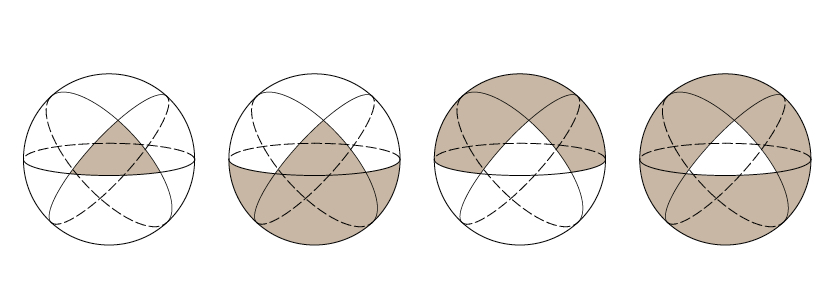
\includegraphics[width=0.9\textwidth]{kugel/Dreieckarten.jpg}
    \captionof{figure}{Dreieckarten auf einer Kugeloberfläche}
\end{center}

Der Begriff Sphärisches Dreieck oder Kugeldreieck ist ein sehr weitläufiger Begriff. 
Dabei können wir den Begriff in drei für uns wesentliche Dreiecke unterteilen:

\begin{itemize}
\item Kugelzweieck
\item Nicht Eulersche’Dreiecke
\item Eulersche’Dreiecke
\end{itemize}

\subsection{Kugelzweieck}

Zwei Grosskreise auf der Kugeloberfläche, zerlegen diese in vier gleiche Kugelzweiecke. 
Jedes dieser Dreieckseiten hat die Länge
$180^{\circ}$ oder $\pi$
Der Flächeninhalt wird dabei nur durch den Winkel $\alpha$ zwischen den beiden Grosskreisen bestimmt.

\begin{center}
        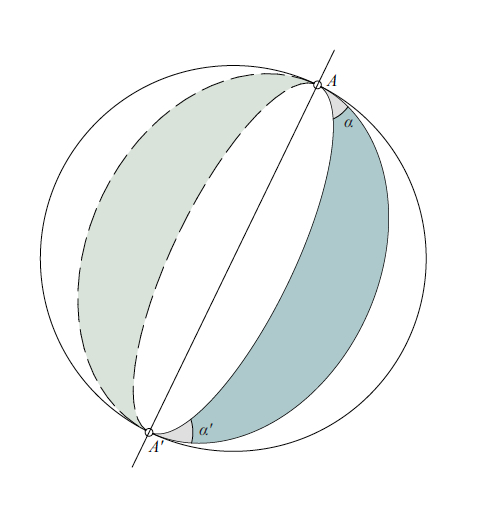
\includegraphics[width=0.3\textwidth]{kugel/Zweieck.jpg}
    \captionof{figure}{Bildung von Zweiecken durch Grosskreise}
\end{center}

Dabei ist der Flächeninhalt der ganzen Kugel:

\begin{align*}
A_{ Kugel } &= 4 \pi r^{2}
\end{align*}


Um den Flächeninhalt des betrachteten Zweieckes zu bekommen, 
müssen wir das ganze noch mit dem Kugelsegment mit dem Winkel $\alpha$ multiplizieren.

\begin{align*}
A_{ Zweieck } &= 4 \pi r^{2} \cdot \frac{ \alpha }{ 2 \pi }
\end{align*}


\subsection{Nicht Eulersche’ Dreiecke}

BLABLA

\subsection{Eulersche’ Dreiecke}

Legt man drei Grosskreise auf eine Kugeloberfläche, bilden sich dabei acht Dreiecke. 
Ein solches Dreieck heisst Eulersches’Dreieck\footnote{%
Leonard Euler (1707-1783), berühmter Schweizer Mathematiker und Physiker. 
Nicht Eulersche’Dreiecke erhält man, indem man das Äussere des Dreieckes ABC betrachtet.} 
Diese Dreiecke werden weder durch die Verlängerung ihrer Seiten durchschnitten, 
noch haben sie Dreiecksseiten welche grösser als $180^{\circ}$ sind.

\begin{center}
        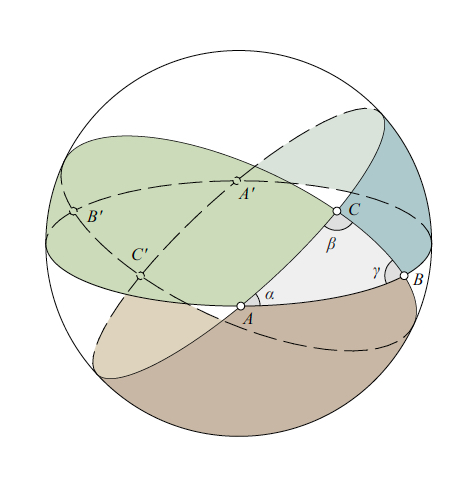
\includegraphics[width=0.4\textwidth]{kugel/Zweiecke.jpg}
    \captionof{figure}{Drei Grosskreise bilden ein sphärisches Dreieck}
\end{center}

In den nachstehenden Erklärungen und Herleitungen, sprechen wir ausschliesslich von Eulerschen’Dreiecken, da die umgeformten Winkelsätze der ebenen Trigonometrie nur auf diese Art von Kugeldreiecken angewendet werden kann.

$A_{ \overline{ ABC }}$ ist die Fläche des Dreieckes auf der Kugeloberfläche
In der ebenen Trigonometrie liegt die Winkelsumme eines Dreiecks bei
$180^{\circ}$.

Anders aber in der sphärischen Trigonometrie. Obschon sie einige Gemeinsamkeiten zur ebenen Trigonometrie aufweist, kann man nicht alles übernehmen.
So auch nicht wie Winkelsumme in einem sphärischen Dreieck.
Diese liegt bei:

\[
\begin{aligned}
\pi
&-
3\pi
&
&\text{\bigg \vert}
&
180^{\circ}
&-
540^{\circ}
\end{aligned}
\]

daraus lässt sich ableiten, das ein einzelner Winkel nicht grösser als $\pi$ oder $180^{\circ}$ sein darf. Ansonsten ist es kein Eulersches’Dreieck und wir dürfen die sphärische Trigonometrie nicht anwenden.\\
Wichtig anzumerken ist, dass die Seiten immer in Radiant beschrieben werden und nicht im Längenmass Meter wie wir es uns gewohnt sind. 
Bei den Dreiecksseiten handelt es sich um Kreisbögen und keine Strecken.

\section{Dreiecksfläche}

\begin{align*}
\text{Zweieck A}
&=
\overline{ABC} + \overline{A'BC} = 2 \alpha r^{ 2 } = A_{ \alpha }\\
\text{Zweieck B}
&=
\overline{ABC} + \overline{AB'C} = 2 \beta r^{ 2 } = A_{ \beta }\\
\text{Zweieck C}
&=
\overline{ABC} + \overline{ABC'} = 2 \gamma r^{ 2 } = A_{ \gamma }
\end{align*}

\begin{align*}
A_{ \alpha } + A_{ \beta } + A_{ \gamma } &= \frac{ 4\pi r^{ 2 } }{ 2 } + 2A_{ \overline{ ABC }} \\
2\alpha r^{ 2 } + 2\beta r^{ 2 } + 2\gamma r^{ 2 } &= \frac{ 4\pi r^{ 2 } }{ 2 } + 2A_{ \overline{ ABC }} \parallel:2\\
\alpha r^{ 2 } + \beta r^{ 2 } + \gamma r^{ 2 } &= \pi r^{ 2 } + A_{ \overline{ ABC }} \parallel-\pi r^{ 2 }\\
r^{ 2 }\left(\alpha + \beta + \gamma - \pi\right) &= A_{ \overline{ ABC }}
\end{align*}




\section{Sphärischer Exzess}
Die Winkelsumme sphärischer Dreiecke ist immer \textgreater \,  $\pi$.

\begin{align*}
\pi < \alpha + \beta + \gamma
\end{align*}

Der sphärische Exzess gibt dabei an, wie stark die Winkelsumme von $\pi$ abweicht.

\begin{align*}
\pi + \epsilon &= \alpha + \beta + \gamma \\
\epsilon &= \alpha + \beta + \gamma - \pi
\end{align*}

Würde der sphärische Exzess in der ebenen Trigonometrie angewendet, wäre dieser = 0. 
Bezieht man das auf die Erde und somit einer Kugel, kann man mit Hilfe eines beliebigen sphärischen Dreieckes und dessen Flächeninhalt auf den Radius der Kugel schliessen.

\subsection{Grenzfall - Satz von Legendre}

\begin{quote} \textit{Ein kleines sphärisches Dreieck kann näherungsweise 
wie ein ebenes Dreieck mit denselben Seiten berechnet 
werden, wenn alle Winkel des ebenen Dreiecks die um 
je ein Drittel des sphärischen Exzesses verminderten 
Winkel des sphärischen Dreiecks nimmt.} \end{quote}
\begin{flushright} - Adrien-Marie Legendre (1752-1833), Paris 1787
\end{flushright}x

Diese Aussage zeigt den Zusammenhang zwischen der 
Trigonometrie in der Ebene sowie in auf der Kugel
auf. Im speziellen bei sehr kleinen sphärischen 
Dreiecken ist die Winkelsumme nur unwesentlich 
grösser als $180^{\circ}$. Des Weiteren kann gesagt werden,
dass der sphärische Exzess gleichmässig auf alle
Winkel aufgeteilt wird.
Wichtig anzumerken ist, dass der Satz von Legendre 
für grosse, aber endliche Radien $r$ gilt.

%[SKIZZE GROSSER RADIUS/KLEINE KRÜMMUNG, KLEINER RADIUS/GROSSE KRÜMMUNG!!!!]
%


\section{Sphärisch Analoge Winkelfunktionen}

\subsection{Sphärischer Sinussatz}

Wir stellen die allgemeinen Sinussätze der Winkel $\alpha$ und $\gamma$ auf:


\[
\begin{aligned}
&{sin(\gamma)} = \frac{h}{a}
&
&\text{\bigg \vert}
&
&{sin(\alpha)} = \frac{h}{c}
&
\end{aligned}
\]

Daraus folgt:
\begin{align*}
h &= sin(\gamma)\cdot a \\
h &= sin(\alpha)\cdot c
\end{align*} 

Durch Gleichsetzung erhält man:
\begin{align*}
h &= h \\
sin(\gamma)\cdot a &= sin(\alpha)\cdot c
\end{align*} 

Durch umstellen erhalten wir den Sinussatz für a und c:
\begin{align*}
sin(\gamma)\cdot a &= sin(\alpha)\cdot c \\
\frac{sin(\gamma)}{c} &= \frac{sin(\alpha)}{a} 
\end{align*} 



\begin{align*}
\frac{sin(\alpha)}{sin(a)} = \frac{sin(\beta)}{sin(b)} = \frac{sin(\gamma)}{sin(c)}
\end{align*} 


\subsection{Winkelkosinussatz}

%[SKIZZE WINKELKOSINUS]

\[
\begin{aligned}
&\overline{C'A'} &= d\cdot {tan(b)}
&
&
&
&
&
&\overline{C'B'} &= d\cdot {tan(a)}
\end{aligned}
\]

\[
\begin{aligned}
&\overline{MA'} &= \frac{ d }{cos(b)}
&
&
&
&
&
&\overline{MB'} &= \frac{ d }{cos(a)}
\end{aligned}
\]

Der allgemeine Kosinussatz beschreibt sich wie folgt:

\begin{align*}
c^{ 2 } &= a^{ 2 } + b^{ 2 } - 2ab \cdot cos(\gamma)
\end{align*}

\begin{align*}
\triangle \overline{A'B'C' }
\overline{ A'B' }^{ 2 } &= \overline{ C'B' }^{ 2 } + \overline{ C'A' }^{ 2 } - 2 \cdot \overline{ C'B' } \cdot \overline{ C'A' } \cdot cos(\gamma)
\end{align*}



\begin{align*}
\overline{A'B'}^{ 2 } &= (d\cdot tan(a))^{ 2 } + (d\cdot tan(b))^{ 2 } - 2 \cdot (d\cdot tan(a) \cdot (d\cdot tan(b) \cdot cos(\gamma)\\
\overline{A'B'}^{ 2 } &= d^{ 2 } \cdot \left(\left(tan^{ 2 }(a) + tan^{ 2 }(b)\right) - 2\cdot tan(a) \cdot tan(b) \cdot cos(\gamma)\right)
\end{align*}

\begin{align*}
\triangle \overline{ MA'B' }
\overline{ A'B' }^{ 2 } &= \overline{ MB' }^{ 2 } + \overline{ MA' }^{ 2 } - 2\cdot \overline{ MB'} \cdot \overline{ MA' } \cdot cos(c)
\end{align*}


\begin{align*}
\overline{ A'B'}^{ 2 } &= \left(\frac{ d }{ cos(a) }  \right)^{ 2 } + \left(\frac{ d }{ cos(b)}  \right)^{ 2 } - 2 \cdot \frac{ d }{ cos(a)} \cdot \frac{ d }{ cos(b)} \cdot cos(c) \\
\overline{ A'B' }^{ 2 } &= d^{ 2 } \cdot \left(\left(\frac{ 1 }{ cos(a) }  \right)^{ 2 } + \left(\frac{ 1 }{ cos(b) }  \right)^{ 2 } - 2 \cdot \frac{ 1 }{ cos(a)} \cdot \frac{ 1 }{ cos(b)} \cdot cos(c)\right)\\
\overline{ A'B' }^{ 2 } &= d^{ 2 } \cdot \left(\left(tan^{ 2 }(a) + 1\right) + \left(tan^{ 2 }(b) + 1\right) - \left(2 \cdot \frac{cos(c)}{cos(a) \cdot cos(b)}\right)\right)
\end{align*}



\begin{align*}
\overline{ A'B'}^{ 2 } &= d^{ 2 } \cdot \left(\left(tan^{ 2 }(a) + tan^{ 2 }(b)\right) - 2 \cdot tan(a) \cdot tan(b) \cdot cos(\gamma)\right) \\
\overline{ A'B'}^{ 2 } &= d^{ 2 } \cdot \left(\left(tan^{ 2 }(a) + 1\right) + \left(tan^{ 2 }(b) + 1\right) - \left(2 \cdot \frac{cos(c)}{cos(a) \cdot cos(b)}\right)\right)
\end{align*}

Die anderen Gleichungen des Satzes, erfolgen aus Symmetriegründen.

\subsection{Seitenkosinussatz}
Durch zyklische Vertauschung des Winkelkosinus erhalten wir den Seitenkosinussatz:

\begin{align*}
{cos(a)} &= {cos(b)} \cdot {cos(c)} + {sin(b)} \cdot {sin(c)} \cdot {sin(\alpha)}\\
{cos(b)} &= {cos(a)} \cdot {cos(c)} + {sin(a)} \cdot {sin(c)} \cdot {sin(\beta)}\\
{cos(c)} &= {cos(a)} \cdot {cos(b)} + {sin(a)} \cdot {sin(b)} \cdot {sin(\gamma)}\\
\end{align*}

\section{Navigation auf See}
Das besondere an Seekarten ist die Inhaltliche Ausrichtung. Anders wie Landkarten muss sie Informationen enthalten welche für den Kapitän und seine Besatzung von grosser Bedeutung sind. Vor allem in Küstennähe ist das navigieren eines Schiffes besonders gefährlich. So enthalten Seekarten etwas über Wassertiefen, Bodenbeschaffenheiten, Gezeiten, Küstenlinien, Landzungen und Windrichtungen.
Der Hauptunterschied dabei ist, das auf der Landkarte feste Positionen definiert und aufgezeigt werden, das einzige was sich verändert ist der Reisende selbst. Bei der Seekarte ist das anders, es werden veränderliche Einwirkungen der Natur festgehalten.

Dieser kleine Unterschied zeigt die Notwendigkeit auf, die Position und den Kurs seines Schiffes auf See immer ermitteln zu können.


\section{Geographische Koordinaten}

Nachdem klar war, das die Erde eine Kugel ist, wurde diese in ein Gradnetz aufgeteilt. Dabei wurden die Angaben für eine exakte Ortsbestimmung klar definiert und die bis heute gültigen Koordinaten bestimmt.
Dabei muss man sich nochmals in Erinnerung rufen, dass sich die Erde in 24h einmal um ihre eigene Achse dreht. Nach $360 ^{\circ}$ 
und somit einer vollen Umdrehung, steht sie wieder in ihrer Ursprungsposition und ein neuer Tag beginnt.

Die Koordinaten setzen sich aus folgenden Komponenten zusammen:

\[
\begin{aligned}
&\text{Grad } (^{\circ})
&
&\text{\bigg \vert}
&
&\text{Bogenminuten } (`)
&
&\text{\bigg \vert}
&
&\text{Bogensekunden } (``)
\end{aligned}
\]

Die Erdoberfläche wurde in je 360 Breiten- und Längengrade eingeteilt. Die Breitengrade haben zueinander einen Abstand von 111.31 km, dies entspricht auch dem Abstand der Längengrade am Äquator mit Zunehmender Nähe zu den Polen, nimmt dieser Abstand ab.

\[
\begin{aligned}
&1^{\circ}
&
&\text{\bigg \vert}
&
&4 \text{ Minuten}
&
&\text{\bigg \vert}
&
&111.31\text{ km}
\end{aligned}
\]

Berechnet man nun die Erdumdrehung von 360°, erhält man genau den Erdumfang am Äquator: \begin{align*} 40’074 \text{ km.}\end{align*}

Dabei geben die Bogenminuten und -sekunden dem Standort die gewünschte Exaktheit. Mit den vollständigen Koordinaten lässt sich der Standort auf einer Landkarte exakt bestimmen und einzeichnen.

\subsection{Zeitzonen der Erde}
Wenn man nun die verschiedenen Zeitzonen der Erde betrachtet, macht die Verschiebung von jeweils einer Stunde durchaus Sinn, es lässt sich auf die Längengrade schliessen.
Zwischen den verschiedenen Zeitzonen liegen 15 Längengrade:

\begin{align*}
\text{15 Längengrade à 4 Minuten = 60 Minuten Zeitverschiebung = ca. 1665 km}
\end{align*}

Dabei ist die Zeitzone in welcher Mitte sich der Greenwich Meredian befindet die \textit{Greenwich Mean Time (GMT)} welche bis 1928 als Weltzeit galt. Im Jahr 1972 wurde diese umbenannt in die \textit{Coordinated Universal Time (UTC)} und wir von da an als Weltzeit $\pm$ 0.00 verwendet.


\section{Der Breitengrad}
Die Breitengrade bilden die bereits genannten Kleinkreise auf der Kugeloberfläche. Sie verlaufen in einem Abstand von genau 111 km parallel zum Äquator. Dabei stellt  dieser genau die Mitte zwischen Nord- und Südpol dar und teilt die Erdkugel in zwei gleiche Hälften. Somit wird von nördlicher und südlicher Breite gesprochen, je nach dem auf welcher Halbkugel man sich befindet.

%[SKIZZE DER GEOGRAFISCHEN BREITE ERDKUGEL]

\subsection{Geografische Breite $\phi$}
\begin{definition}
Die geografische Breite eines Standortes ist nichts anderes, als der Winkel am Erdmittelpunkt zwischen der Ebene des Äquators und der Geraden zum Standpunkt auf der Erdoberfläche.
\end{definition}

%[SKIZZE DER GEOGRAFISCHEN BREITE MIT WINKEL]

\subsection{Navigation mit den Breitengraden}
Da der Breitengrad bereits sehr früh ziemlich präzise bestimmt werden könnte, nutzten bereits die Seefahrer um Christoph Kolumbus den Breitengrad zur Navigation ihrer Flotten.
Den dieser lässt sich ziemlich einfach aus dem höchsten Sonnenstand oder einem Fixstern bestimmen. Dabei wird mit einem Jakobsstab\footnote{%
Der Jakobsstab ist ein früheres astronomisches Instrument zur Winkelmessung und wurde vor allem in der Seefahrt verwendet. Er ist in der Nautik der Vorläufer des Sextanten.} (später Sextant\footnote{%
Der Sextant ist ein nautisches Messinstrument zur Winkelmessung von Horizont und Fixstern (Gestirn)}) der Winkel zwischen dem Horizont und dem Fixstern gemessen. Der Winkel welchen man erhält, zieht man von 90° ab und erhält somit die geografische Breite. \\

%[SKIZZE ERMITTLUNG DES BREITENGRADES]

Wenn man sich auf der Nordhalbkugel befindet, ist der Polarstern ein sehr guter Fixstern. Befindet sich ein Schiff nun sehr nahe am Nordpol, steht dieser nahezu senkrecht am Himmelszelt bei $90^{\circ}$. Würde es aber nahe dem Äquator stehen, erscheint dieser am Horizont bei $0^{\circ}$.

\subsection{Korrekturbeiwert}

\section{Der Längengrad}
Die Längengrade bilden die bereits genannten Grosskreise auf der Kugeloberfläche.
Sie schneiden den Äquator im rechten Winkel, haben dort einen Abstand von 111 km zueinander und verbinden die Pole. Anders wie bei der geografischen Breite, ist in der Natur kein Längengrad gegeben welcher den Nullpunkt darstellt.

%[SKIZZE DER GEOGRAFISCHEN LÄNGE ERDKUGEL]

\subsection{Geografische Länge $\lambda$}
\begin{definition}
Die geografische Länge ist der Winkel an der Erdachse zum Nullmeridian.
\end{definition}

\subsection{Navigation mit den Längengraden}
Die geografische Länge lässt sich nicht so einfach bestimmen wie deren Breite. Für die Berechnung auf See benötigt man eine Referenzzeit eines Ortes mit bekannter Länge.
In der Zeit der Entdecker gab es noch keine mechanischen Uhren. Die Sonnenuhr war zudem ungeeignet, da diese nur die Uhrzeit am Standort mass und nicht die am Referenzort selbst. Die erste Pendeluhr wurde erst Mitte des 17. Jahrhunderts erfunden, was in der Schifffahrt aber auch nicht die Lösung brachte.\\
Pendeluhren auf einem Schiff sind ungeeignet, da das Pendel mit dem Wellengang aus dem Takt gebracht wird und somit die Uhr falsch geht.
Zu ungenau und gegen äussere Erschütterungen zu empfindlich waren später auch die federgetriebenen Uhren und die Unruh. Dazukamen die verschiedenen Klimazonen welche ein Schiff zu durchqueren hatten. Das Metall zog sich viel zu fest zusammen oder dehnte sich aus, was dazu führte das die Uhr unregelmässig lief.

Das sogenannte „Längenproblem“ stellte nicht nur bei der Navigation auf See ein Problem dar, es ergaben sich auch wirtschaftliche Konsequenzen. Die Schiffe mussten bis zur gewünschten geografischen Breite navigieren und segelten dann den Breitengrad entlang. Dabei waren die Schiffe oft Wochenlang unterwegs und segelten die „Breiten ab“ um an die gewünschte Position zu kommen. Dies führte zu erheblichen Zeitverlusten und viel längeren Reisezeiten.


\section{The Board of Longitude - Das Längenproblem}
Das Längenproblem beschäftigte alle grossen Seefahrernationen Europas. Wenn man bedenkt das sich Werte in einer  Höhe von halben britischen Staatshaushalten auf verloren gegangenen Schiffen befanden, erkennt man die Dringlichkeit für eine zuverlässige und genaue Navigation auf See.


\begin{itemize}
\item £ 20’000 - Abweichung von max. einem halben Grad
\item £ 15’000 - Abweichung von zwei Drittel Grad
\item £ 10’000 - Abweichung von max. $1 ^{\circ}$
\end{itemize}

\subsection{John Harrison}


\subsection{Tobias Mayer}



Uhren mit einer Abweichung von einer Minute Abweichung pro Tag (





\section{Nautische Dreieck}


$\Rightarrow$





\section{Die Vermessung der Welt}
Wir schreiben das Jahr 1818 und kehren in die Zeit des Mathematikers Carl Friedrich Gauss zurück. Neben dem liebevoll genannten „kleinen Gauss“ und anderen herausragenden Mathematischen Leistungen, beschäftigte er in den Folgejahren mit der Vermessung des Königreichs Hannovers und verfasste auf 61 Blättern das Kartenwerk \textit{Gauss’sche Landesaufnahme der 1815 durch Hannover erworbenen Gebiete}.






AUFGABE

Hubble Teleskop 
24. April 1990






\printbibliography[heading=subbibliography]
\end{refsection}




%\chapter{Geometrie auf der Kugeloberfläche\label{chapter:kugel}}
\lhead{Geometrie auf der Kugeloberfläche}
\begin{refsection}
\chapterauthor{Melina Staub und Fabian Schmid}

\section{Einleitung}

Schon seit jeher fasziniert den Menschen die Fahrt zur See. Nicht grundlos ist die Seefahrt eine der wichtigsten und ältesten Tätigkeiten der Menschheit. Der innerliche Drang neue Weltmeere und unbekannte Gebiete zu entdecken, die Fahrt zur See zu erleichtern und erträglicher zu machen, trieben die Menschen an, die Schiffe dieser Welt immer weiter zu entwickeln.

Die Idee der Kugelform der Erde ist älter als man zu denken vermag. Bereits der Schüler des antiken griechischen Philosophen Platon - Aristoteles schrieb in seiner Schrift \textit{Über den Himmel} aus dem 4. Jahrhundert v. Chr. etliche Gründe welche für die Gestallt der Erde als Kugel sprechen:

\begin{itemize}
      \item Sämtliche schweren Körper streben zum Mittelpunkt des Alls. Da sie dies von allen Seiten her gleichmäßig tun und die Erde im Mittelpunkt des Alls steht, muss sie eine kugelrunde Gestalt annehmen. 
\item Bei von der Küste wegfahrende Schiffen wird der Rumpf vor den Segeln der Sicht verborgen. 
\item In südlichen Ländern erscheinen südliche Sternbilder höher über dem Horizont.
\item Der Erdschatten bei einer Mondfinsternis ist stets rund.
\end{itemize}

Jedoch war um 1492 - der Zeit der Entdeckung Amerikas durch Christoph Kolumbus, die Idee der Erde in Kugelform noch sehr umstritten. Er erkannte anhand den Theorien und Erkenntnissen der alten Griechen, vor allem Aristoteles, das die Erde eine Kugel sein muss. \\
Doch mit seinem Vorschlag einen Seeweg über den Atlantik nach Indien zu finden und nicht wie üblich um Afrika zu segeln, stiess er beim beim portugiesischen König auf taube Ohren. Sein Plan Indien über eine Route nach Westen zu erreichen, widersprach dem gesunden Menschenverstand. Wäre die Erde wirklich eine Kugel und man befände sich auf der unteren Erdhalbkugel, würde man herunterfallen.\\
Doch auch der damals übliche Glaube an die Erde in Scheibenform brachte so einige Risiken mit sich. Was würde passieren, wenn die Flotte das Ende der Scheibe erreicht hatte? Würden sie über den Erdrand hinweggleiten und in den Abgrund stürzen?\\
Erst nach viel Überzeugungsarbeit durch Kolumbus, setzte er sich am Spanischen Hof durch und segelte über die Westliche Route über den Atlantik und entdeckte schlussendlich Amerika.

Der praktische und greifbare Beweis das die Erde eine Kugel ist, lieferte rund 30 Jahre später der Portugiese Fernando Magellan. Mit seiner Weltumsegelung und seiner Ankunft in den Philippinen, bewies er definitiv das die Erde eine Kugel ist.\\

Nun wollen wir uns die Frage stellen, wie die alten Seefahrer ohne GPS und jeglichen modernen Navigationssystemen auf hoher See wussten wo sie sich befinden und was haben die Sterne mit alldem zu tun? Reisen Sie mit uns zurück in eine Zeit mit Sextant, Kompass und Sternkarten. In die Zeit der Seefahrer und Entdecker.


\section{Geometrie auf der Ebene und der Kugel}

Euklid von Alexandria beschrieb die Grundbegriffe der ebenen Geometrie mittels Punkt, Geraden, Ebene, Winkel und Dreieck. Diese Dreiecke lassen sich mithilfe der ebenen Trigonometrie beschreiben. Dabei gelten die uns bekannten trigonometrischen Winkelfunktionen:\\

\text{Sinussatz:}
\begin{align*}
\frac{ a }{ sin(\alpha) } &= \frac{ b }{sin(\beta)} = \frac{ c }{ sin(\gamma) } = \frac{abc}{2A} = 2r\\
\end{align*}

\text{Cosinussatz:}
\begin{align*}
c^{ 2 } &= a^{ 2 } + b^{ 2 } - 2ab\cdot cos(\gamma)\\
b^{ 2 } &= a^{ 2 } + c^{ 2 } - 2ab\cdot cos(\beta)\\
a^{ 2 } &= b^{ 2 } + c^{ 2 } - 2ab\cdot cos(\alpha)
\end{align*}

Um Dreiecke auf der Kugeloberfläche zu berechnen, benötigt man die sphärische Trigonometrie. Die oben beschriebenen Sätze lassen sich auf der Kugel nicht anwenden, sie werden aber als Grundlage zur Herleitung der Sätze für das Kugeldreieck benötigt.

Die nachfolgenden Seiten thematisieren die Geometrie auf der Kugeloberfläche und wie sie in der Navigation eingesetzt werden kann.


\section{Gross- und Kleinkreise}

Eine Kugeloberfläche lässt sich in zwei verschiedene Kreisarten einteilen -  Gross- und Kleinkreise. 
Wir betrachten als erstes die Grosskreise:

\begin{definition}
Ein Großkreis ist ein größtmöglicher Kreis auf einer Kugeloberfläche. Sein Mittelpunkt fällt immer mit dem Mittelpunkt der Kugel zusammen und ein Schnitt auf dem Großkreis teilt die Kugel in jedem Fall in zwei („gleich große“) Hälften.
\end{definition}

Es gibt unendlich viele Möglichkeiten, eine Kugel in zwei gleich grosse Stücke zu zerschneiden, 
daher gibt es auch unendlich viele Grosskreise. Wenn wir die Grosskreise auf einer Kugel mit diesen auf der Erde beschreiben, sprechen wir von den Längengraden aber auch der Äquator beschreibt einen Grosskreis.
Ein Elementarer Bestandteil bilden die Grosskreise in der sphärischen Trigonometrie. Mithilfe der Schnittpunkte verschiedener Grosskreise, lässt sich ein Sphärisches Dreieck bilden auf welchem sich die sphärische Trigonometrie anwenden lässt.

[GRAFIK GROSSKREISE]

\begin{definition}
Unter Kleinkreis versteht man jene Kreise auf einer Kugeloberfläche, deren Ebenen nicht den Kugelmittelpunkt enthalten.
\end{definition}

Die Kleinkreise eignen sich im Gegensatz zu den Grosskreisen \textit{nicht} für die sphärische Trigonometrie. 
Sie werden lediglich zur Bestimmung der Messgrössen, Winkelabstände oder des Höhenwinkels eines Gestirns verwendet. 

Wenn wir die Kleinkreise auf die Erdoberfläche projizieren betrachten wir die Breitengrade.

[GRAFIK KLEINKREISE]


\section{Sphärische Dreiecke / Kugeldreieck}

\begin{center}
        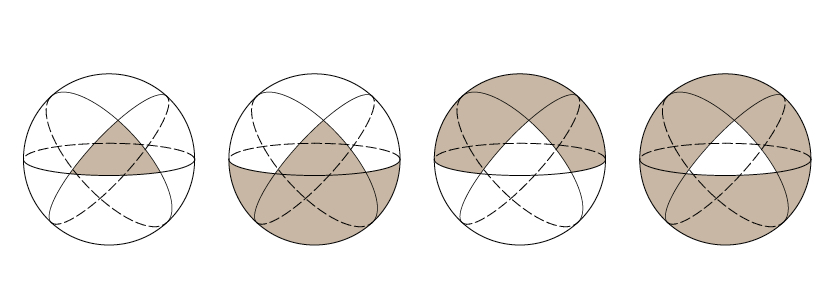
\includegraphics[width=0.9\textwidth]{kugel/Dreieckarten.jpg}
    \captionof{figure}{Dreieckarten auf einer Kugeloberfläche}
\end{center}

Der Begriff Sphärisches Dreieck oder Kugeldreieck ist ein sehr weitläufiger Begriff. 
Dabei können wir den Begriff in drei für uns wesentliche Dreiecke unterteilen:

\begin{itemize}
\item Kugelzweieck
\item Nicht Eulersche’Dreiecke
\item Eulersche’Dreiecke
\end{itemize}

\subsection{Kugelzweieck}

Zwei Grosskreise auf der Kugeloberfläche, zerlegen diese in vier gleiche Kugelzweiecke. 
Jedes dieser Dreieckseiten hat die Länge
$180^{\circ}$ oder $\pi$
Der Flächeninhalt wird dabei nur durch den Winkel $\alpha$ zwischen den beiden Grosskreisen bestimmt.

\begin{center}
        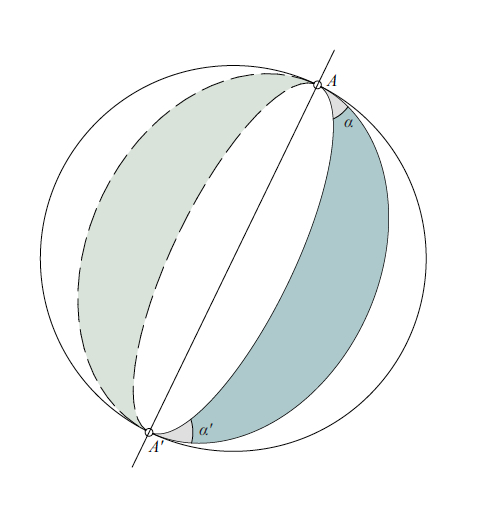
\includegraphics[width=0.3\textwidth]{kugel/Zweieck.jpg}
    \captionof{figure}{Bildung von Zweiecken durch Grosskreise}
\end{center}

Dabei ist der Flächeninhalt der ganzen Kugel:

\begin{align*}
A_{ Kugel } &= 4 \pi r^{2}
\end{align*}


Um den Flächeninhalt des betrachteten Zweieckes zu bekommen, 
müssen wir das ganze noch mit dem Kugelsegment mit dem Winkel $\alpha$ multiplizieren.

\begin{align*}
A_{ Zweieck } &= 4 \pi r^{2} \cdot \frac{ \alpha }{ 2 \pi }
\end{align*}


\subsection{Nicht Eulersche’ Dreiecke}

BLABLA

\subsection{Eulersche’ Dreiecke}

Legt man drei Grosskreise auf eine Kugeloberfläche, bilden sich dabei acht Dreiecke. 
Ein solches Dreieck heisst Eulersches’Dreieck\footnote{%
Leonard Euler (1707-1783), berühmter Schweizer Mathematiker und Physiker. 
Nicht Eulersche’Dreiecke erhält man, indem man das Äussere des Dreieckes ABC betrachtet.} 
Diese Dreiecke werden weder durch die Verlängerung ihrer Seiten durchschnitten, 
noch haben sie Dreiecksseiten welche grösser als $180^{\circ}$ sind.

\begin{center}
        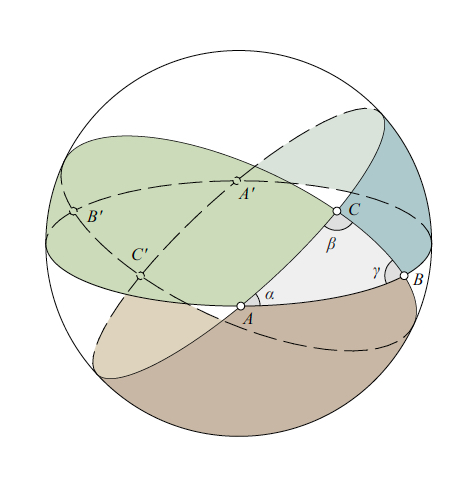
\includegraphics[width=0.4\textwidth]{kugel/Zweiecke.jpg}
    \captionof{figure}{Drei Grosskreise bilden ein sphärisches Dreieck}
\end{center}

In den nachstehenden Erklärungen und Herleitungen, sprechen wir ausschliesslich von Eulerschen’Dreiecken, da die umgeformten Winkelsätze der ebenen Trigonometrie nur auf diese Art von Kugeldreiecken angewendet werden kann.

$A_{ \overline{ ABC }}$ ist die Fläche des Dreieckes auf der Kugeloberfläche
In der ebenen Trigonometrie liegt die Winkelsumme eines Dreiecks bei
$180^{\circ}$.

Anders aber in der sphärischen Trigonometrie. Obschon sie einige Gemeinsamkeiten zur ebenen Trigonometrie aufweist, kann man nicht alles übernehmen.
So auch nicht wie Winkelsumme in einem sphärischen Dreieck.
Diese liegt bei:

\[
\begin{aligned}
\pi
&-
3\pi
&
&\text{\bigg \vert}
&
180^{\circ}
&-
540^{\circ}
\end{aligned}
\]

daraus lässt sich ableiten, das ein einzelner Winkel nicht grösser als $\pi$ oder $180^{\circ}$ sein darf. Ansonsten ist es kein Eulersches’Dreieck und wir dürfen die sphärische Trigonometrie nicht anwenden.\\
Wichtig anzumerken ist, dass die Seiten immer in Radiant beschrieben werden und nicht im Längenmass Meter wie wir es uns gewohnt sind. 
Bei den Dreiecksseiten handelt es sich um Kreisbögen und keine Strecken.

\section{Dreiecksfläche}

\begin{align*}
\text{Zweieck A}
&=
\overline{ABC} + \overline{A'BC} = 2 \alpha r^{ 2 } = A_{ \alpha }\\
\text{Zweieck B}
&=
\overline{ABC} + \overline{AB'C} = 2 \beta r^{ 2 } = A_{ \beta }\\
\text{Zweieck C}
&=
\overline{ABC} + \overline{ABC'} = 2 \gamma r^{ 2 } = A_{ \gamma }
\end{align*}

\begin{align*}
A_{ \alpha } + A_{ \beta } + A_{ \gamma } &= \frac{ 4\pi r^{ 2 } }{ 2 } + 2A_{ \overline{ ABC }} \\
2\alpha r^{ 2 } + 2\beta r^{ 2 } + 2\gamma r^{ 2 } &= \frac{ 4\pi r^{ 2 } }{ 2 } + 2A_{ \overline{ ABC }} \parallel:2\\
\alpha r^{ 2 } + \beta r^{ 2 } + \gamma r^{ 2 } &= \pi r^{ 2 } + A_{ \overline{ ABC }} \parallel-\pi r^{ 2 }\\
r^{ 2 }\left(\alpha + \beta + \gamma - \pi\right) &= A_{ \overline{ ABC }}
\end{align*}




\section{Sphärischer Exzess}
Die Winkelsumme sphärischer Dreiecke ist immer \textgreater \,  $\pi$.

\begin{align*}
\pi < \alpha + \beta + \gamma
\end{align*}

Der sphärische Exzess gibt dabei an, wie stark die Winkelsumme von $\pi$ abweicht.

\begin{align*}
\pi + \epsilon &= \alpha + \beta + \gamma \\
\epsilon &= \alpha + \beta + \gamma - \pi
\end{align*}

Würde der sphärische Exzess in der ebenen Trigonometrie angewendet, wäre dieser = 0. 
Bezieht man das auf die Erde und somit einer Kugel, kann man mit Hilfe eines beliebigen sphärischen Dreieckes und dessen Flächeninhalt auf den Radius der Kugel schliessen.

\subsection{Grenzfall - Satz von Legendre}

\begin{quote} \textit{Ein kleines sphärisches Dreieck kann näherungsweise 
wie ein ebenes Dreieck mit denselben Seiten berechnet 
werden, wenn alle Winkel des ebenen Dreiecks die um 
je ein Drittel des sphärischen Exzesses verminderten 
Winkel des sphärischen Dreiecks nimmt.} \end{quote}
\begin{flushright} - Adrien-Marie Legendre (1752-1833), Paris 1787
\end{flushright}x

Diese Aussage zeigt den Zusammenhang zwischen der 
Trigonometrie in der Ebene sowie in auf der Kugel
auf. Im speziellen bei sehr kleinen sphärischen 
Dreiecken ist die Winkelsumme nur unwesentlich 
grösser als $180^{\circ}$. Des Weiteren kann gesagt werden,
dass der sphärische Exzess gleichmässig auf alle
Winkel aufgeteilt wird.
Wichtig anzumerken ist, dass der Satz von Legendre 
für grosse, aber endliche Radien $r$ gilt.

%[SKIZZE GROSSER RADIUS/KLEINE KRÜMMUNG, KLEINER RADIUS/GROSSE KRÜMMUNG!!!!]
%


\section{Sphärisch Analoge Winkelfunktionen}

\subsection{Sphärischer Sinussatz}

Wir stellen die allgemeinen Sinussätze der Winkel $\alpha$ und $\gamma$ auf:


\[
\begin{aligned}
&{sin(\gamma)} = \frac{h}{a}
&
&\text{\bigg \vert}
&
&{sin(\alpha)} = \frac{h}{c}
&
\end{aligned}
\]

Daraus folgt:
\begin{align*}
h &= sin(\gamma)\cdot a \\
h &= sin(\alpha)\cdot c
\end{align*} 

Durch Gleichsetzung erhält man:
\begin{align*}
h &= h \\
sin(\gamma)\cdot a &= sin(\alpha)\cdot c
\end{align*} 

Durch umstellen erhalten wir den Sinussatz für a und c:
\begin{align*}
sin(\gamma)\cdot a &= sin(\alpha)\cdot c \\
\frac{sin(\gamma)}{c} &= \frac{sin(\alpha)}{a} 
\end{align*} 



\begin{align*}
\frac{sin(\alpha)}{sin(a)} = \frac{sin(\beta)}{sin(b)} = \frac{sin(\gamma)}{sin(c)}
\end{align*} 


\subsection{Winkelkosinussatz}

%[SKIZZE WINKELKOSINUS]

\[
\begin{aligned}
&\overline{C'A'} &= d\cdot {tan(b)}
&
&
&
&
&
&\overline{C'B'} &= d\cdot {tan(a)}
\end{aligned}
\]

\[
\begin{aligned}
&\overline{MA'} &= \frac{ d }{cos(b)}
&
&
&
&
&
&\overline{MB'} &= \frac{ d }{cos(a)}
\end{aligned}
\]

Der allgemeine Kosinussatz beschreibt sich wie folgt:

\begin{align*}
c^{ 2 } &= a^{ 2 } + b^{ 2 } - 2ab \cdot cos(\gamma)
\end{align*}

\begin{align*}
\triangle \overline{A'B'C' }
\overline{ A'B' }^{ 2 } &= \overline{ C'B' }^{ 2 } + \overline{ C'A' }^{ 2 } - 2 \cdot \overline{ C'B' } \cdot \overline{ C'A' } \cdot cos(\gamma)
\end{align*}



\begin{align*}
\overline{A'B'}^{ 2 } &= (d\cdot tan(a))^{ 2 } + (d\cdot tan(b))^{ 2 } - 2 \cdot (d\cdot tan(a) \cdot (d\cdot tan(b) \cdot cos(\gamma)\\
\overline{A'B'}^{ 2 } &= d^{ 2 } \cdot \left(\left(tan^{ 2 }(a) + tan^{ 2 }(b)\right) - 2\cdot tan(a) \cdot tan(b) \cdot cos(\gamma)\right)
\end{align*}

\begin{align*}
\triangle \overline{ MA'B' }
\overline{ A'B' }^{ 2 } &= \overline{ MB' }^{ 2 } + \overline{ MA' }^{ 2 } - 2\cdot \overline{ MB'} \cdot \overline{ MA' } \cdot cos(c)
\end{align*}


\begin{align*}
\overline{ A'B'}^{ 2 } &= \left(\frac{ d }{ cos(a) }  \right)^{ 2 } + \left(\frac{ d }{ cos(b)}  \right)^{ 2 } - 2 \cdot \frac{ d }{ cos(a)} \cdot \frac{ d }{ cos(b)} \cdot cos(c) \\
\overline{ A'B' }^{ 2 } &= d^{ 2 } \cdot \left(\left(\frac{ 1 }{ cos(a) }  \right)^{ 2 } + \left(\frac{ 1 }{ cos(b) }  \right)^{ 2 } - 2 \cdot \frac{ 1 }{ cos(a)} \cdot \frac{ 1 }{ cos(b)} \cdot cos(c)\right)\\
\overline{ A'B' }^{ 2 } &= d^{ 2 } \cdot \left(\left(tan^{ 2 }(a) + 1\right) + \left(tan^{ 2 }(b) + 1\right) - \left(2 \cdot \frac{cos(c)}{cos(a) \cdot cos(b)}\right)\right)
\end{align*}



\begin{align*}
\overline{ A'B'}^{ 2 } &= d^{ 2 } \cdot \left(\left(tan^{ 2 }(a) + tan^{ 2 }(b)\right) - 2 \cdot tan(a) \cdot tan(b) \cdot cos(\gamma)\right) \\
\overline{ A'B'}^{ 2 } &= d^{ 2 } \cdot \left(\left(tan^{ 2 }(a) + 1\right) + \left(tan^{ 2 }(b) + 1\right) - \left(2 \cdot \frac{cos(c)}{cos(a) \cdot cos(b)}\right)\right)
\end{align*}

Die anderen Gleichungen des Satzes, erfolgen aus Symmetriegründen.

\subsection{Seitenkosinussatz}
Durch zyklische Vertauschung des Winkelkosinus erhalten wir den Seitenkosinussatz:

\begin{align*}
{cos(a)} &= {cos(b)} \cdot {cos(c)} + {sin(b)} \cdot {sin(c)} \cdot {sin(\alpha)}\\
{cos(b)} &= {cos(a)} \cdot {cos(c)} + {sin(a)} \cdot {sin(c)} \cdot {sin(\beta)}\\
{cos(c)} &= {cos(a)} \cdot {cos(b)} + {sin(a)} \cdot {sin(b)} \cdot {sin(\gamma)}\\
\end{align*}

\section{Navigation auf See}
Das besondere an Seekarten ist die Inhaltliche Ausrichtung. Anders wie Landkarten muss sie Informationen enthalten welche für den Kapitän und seine Besatzung von grosser Bedeutung sind. Vor allem in Küstennähe ist das navigieren eines Schiffes besonders gefährlich. So enthalten Seekarten etwas über Wassertiefen, Bodenbeschaffenheiten, Gezeiten, Küstenlinien, Landzungen und Windrichtungen.
Der Hauptunterschied dabei ist, das auf der Landkarte feste Positionen definiert und aufgezeigt werden, das einzige was sich verändert ist der Reisende selbst. Bei der Seekarte ist das anders, es werden veränderliche Einwirkungen der Natur festgehalten.

Dieser kleine Unterschied zeigt die Notwendigkeit auf, die Position und den Kurs seines Schiffes auf See immer ermitteln zu können.


\section{Geographische Koordinaten}

Nachdem klar war, das die Erde eine Kugel ist, wurde diese in ein Gradnetz aufgeteilt. Dabei wurden die Angaben für eine exakte Ortsbestimmung klar definiert und die bis heute gültigen Koordinaten bestimmt.
Dabei muss man sich nochmals in Erinnerung rufen, dass sich die Erde in 24h einmal um ihre eigene Achse dreht. Nach $360 ^{\circ}$ 
und somit einer vollen Umdrehung, steht sie wieder in ihrer Ursprungsposition und ein neuer Tag beginnt.

Die Koordinaten setzen sich aus folgenden Komponenten zusammen:

\[
\begin{aligned}
&\text{Grad } (^{\circ})
&
&\text{\bigg \vert}
&
&\text{Bogenminuten } (`)
&
&\text{\bigg \vert}
&
&\text{Bogensekunden } (``)
\end{aligned}
\]

Die Erdoberfläche wurde in je 360 Breiten- und Längengrade eingeteilt. Die Breitengrade haben zueinander einen Abstand von 111.31 km, dies entspricht auch dem Abstand der Längengrade am Äquator mit Zunehmender Nähe zu den Polen, nimmt dieser Abstand ab.

\[
\begin{aligned}
&1^{\circ}
&
&\text{\bigg \vert}
&
&4 \text{ Minuten}
&
&\text{\bigg \vert}
&
&111.31\text{ km}
\end{aligned}
\]

Berechnet man nun die Erdumdrehung von 360°, erhält man genau den Erdumfang am Äquator: \begin{align*} 40’074 \text{ km.}\end{align*}

Dabei geben die Bogenminuten und -sekunden dem Standort die gewünschte Exaktheit. Mit den vollständigen Koordinaten lässt sich der Standort auf einer Landkarte exakt bestimmen und einzeichnen.

\subsection{Zeitzonen der Erde}
Wenn man nun die verschiedenen Zeitzonen der Erde betrachtet, macht die Verschiebung von jeweils einer Stunde durchaus Sinn, es lässt sich auf die Längengrade schliessen.
Zwischen den verschiedenen Zeitzonen liegen 15 Längengrade:

\begin{align*}
\text{15 Längengrade à 4 Minuten = 60 Minuten Zeitverschiebung = ca. 1665 km}
\end{align*}

Dabei ist die Zeitzone in welcher Mitte sich der Greenwich Meredian befindet die \textit{Greenwich Mean Time (GMT)} welche bis 1928 als Weltzeit galt. Im Jahr 1972 wurde diese umbenannt in die \textit{Coordinated Universal Time (UTC)} und wir von da an als Weltzeit $\pm$ 0.00 verwendet.


\section{Der Breitengrad}
Die Breitengrade bilden die bereits genannten Kleinkreise auf der Kugeloberfläche. Sie verlaufen in einem Abstand von genau 111 km parallel zum Äquator. Dabei stellt  dieser genau die Mitte zwischen Nord- und Südpol dar und teilt die Erdkugel in zwei gleiche Hälften. Somit wird von nördlicher und südlicher Breite gesprochen, je nach dem auf welcher Halbkugel man sich befindet.

%[SKIZZE DER GEOGRAFISCHEN BREITE ERDKUGEL]

\subsection{Geografische Breite $\phi$}
\begin{definition}
Die geografische Breite eines Standortes ist nichts anderes, als der Winkel am Erdmittelpunkt zwischen der Ebene des Äquators und der Geraden zum Standpunkt auf der Erdoberfläche.
\end{definition}

%[SKIZZE DER GEOGRAFISCHEN BREITE MIT WINKEL]

\subsection{Navigation mit den Breitengraden}
Da der Breitengrad bereits sehr früh ziemlich präzise bestimmt werden könnte, nutzten bereits die Seefahrer um Christoph Kolumbus den Breitengrad zur Navigation ihrer Flotten.
Den dieser lässt sich ziemlich einfach aus dem höchsten Sonnenstand oder einem Fixstern bestimmen. Dabei wird mit einem Jakobsstab\footnote{%
Der Jakobsstab ist ein früheres astronomisches Instrument zur Winkelmessung und wurde vor allem in der Seefahrt verwendet. Er ist in der Nautik der Vorläufer des Sextanten.} (später Sextant\footnote{%
Der Sextant ist ein nautisches Messinstrument zur Winkelmessung von Horizont und Fixstern (Gestirn)}) der Winkel zwischen dem Horizont und dem Fixstern gemessen. Der Winkel welchen man erhält, zieht man von 90° ab und erhält somit die geografische Breite. \\

%[SKIZZE ERMITTLUNG DES BREITENGRADES]

Wenn man sich auf der Nordhalbkugel befindet, ist der Polarstern ein sehr guter Fixstern. Befindet sich ein Schiff nun sehr nahe am Nordpol, steht dieser nahezu senkrecht am Himmelszelt bei $90^{\circ}$. Würde es aber nahe dem Äquator stehen, erscheint dieser am Horizont bei $0^{\circ}$.

\subsection{Korrekturbeiwert}

\section{Der Längengrad}
Die Längengrade bilden die bereits genannten Grosskreise auf der Kugeloberfläche.
Sie schneiden den Äquator im rechten Winkel, haben dort einen Abstand von 111 km zueinander und verbinden die Pole. Anders wie bei der geografischen Breite, ist in der Natur kein Längengrad gegeben welcher den Nullpunkt darstellt.

%[SKIZZE DER GEOGRAFISCHEN LÄNGE ERDKUGEL]

\subsection{Geografische Länge $\lambda$}
\begin{definition}
Die geografische Länge ist der Winkel an der Erdachse zum Nullmeridian.
\end{definition}

\subsection{Navigation mit den Längengraden}
Die geografische Länge lässt sich nicht so einfach bestimmen wie deren Breite. Für die Berechnung auf See benötigt man eine Referenzzeit eines Ortes mit bekannter Länge.
In der Zeit der Entdecker gab es noch keine mechanischen Uhren. Die Sonnenuhr war zudem ungeeignet, da diese nur die Uhrzeit am Standort mass und nicht die am Referenzort selbst. Die erste Pendeluhr wurde erst Mitte des 17. Jahrhunderts erfunden, was in der Schifffahrt aber auch nicht die Lösung brachte.\\
Pendeluhren auf einem Schiff sind ungeeignet, da das Pendel mit dem Wellengang aus dem Takt gebracht wird und somit die Uhr falsch geht.
Zu ungenau und gegen äussere Erschütterungen zu empfindlich waren später auch die federgetriebenen Uhren und die Unruh. Dazukamen die verschiedenen Klimazonen welche ein Schiff zu durchqueren hatten. Das Metall zog sich viel zu fest zusammen oder dehnte sich aus, was dazu führte das die Uhr unregelmässig lief.

Das sogenannte „Längenproblem“ stellte nicht nur bei der Navigation auf See ein Problem dar, es ergaben sich auch wirtschaftliche Konsequenzen. Die Schiffe mussten bis zur gewünschten geografischen Breite navigieren und segelten dann den Breitengrad entlang. Dabei waren die Schiffe oft Wochenlang unterwegs und segelten die „Breiten ab“ um an die gewünschte Position zu kommen. Dies führte zu erheblichen Zeitverlusten und viel längeren Reisezeiten.


\section{The Board of Longitude - Das Längenproblem}
Das Längenproblem beschäftigte alle grossen Seefahrernationen Europas. Wenn man bedenkt das sich Werte in einer  Höhe von halben britischen Staatshaushalten auf verloren gegangenen Schiffen befanden, erkennt man die Dringlichkeit für eine zuverlässige und genaue Navigation auf See.


\begin{itemize}
\item £ 20’000 - Abweichung von max. einem halben Grad
\item £ 15’000 - Abweichung von zwei Drittel Grad
\item £ 10’000 - Abweichung von max. $1 ^{\circ}$
\end{itemize}

\subsection{John Harrison}


\subsection{Tobias Mayer}



Uhren mit einer Abweichung von einer Minute Abweichung pro Tag (





\section{Nautische Dreieck}


$\Rightarrow$





\section{Die Vermessung der Welt}
Wir schreiben das Jahr 1818 und kehren in die Zeit des Mathematikers Carl Friedrich Gauss zurück. Neben dem liebevoll genannten „kleinen Gauss“ und anderen herausragenden Mathematischen Leistungen, beschäftigte er in den Folgejahren mit der Vermessung des Königreichs Hannovers und verfasste auf 61 Blättern das Kartenwerk \textit{Gauss’sche Landesaufnahme der 1815 durch Hannover erworbenen Gebiete}.






AUFGABE

Hubble Teleskop 
24. April 1990






\printbibliography[heading=subbibliography]
\end{refsection}




%\chapter{Geometrie auf der Kugeloberfläche\label{chapter:kugel}}
\lhead{Geometrie auf der Kugeloberfläche}
\begin{refsection}
\chapterauthor{Melina Staub und Fabian Schmid}

\section{Einleitung}

Schon seit jeher fasziniert den Menschen die Fahrt zur See. Nicht grundlos ist die Seefahrt eine der wichtigsten und ältesten Tätigkeiten der Menschheit. Der innerliche Drang neue Weltmeere und unbekannte Gebiete zu entdecken, die Fahrt zur See zu erleichtern und erträglicher zu machen, trieben die Menschen an, die Schiffe dieser Welt immer weiter zu entwickeln.

Die Idee der Kugelform der Erde ist älter als man zu denken vermag. Bereits der Schüler des antiken griechischen Philosophen Platon - Aristoteles schrieb in seiner Schrift \textit{Über den Himmel} aus dem 4. Jahrhundert v. Chr. etliche Gründe welche für die Gestallt der Erde als Kugel sprechen:

\begin{itemize}
      \item Sämtliche schweren Körper streben zum Mittelpunkt des Alls. Da sie dies von allen Seiten her gleichmäßig tun und die Erde im Mittelpunkt des Alls steht, muss sie eine kugelrunde Gestalt annehmen. 
\item Bei von der Küste wegfahrende Schiffen wird der Rumpf vor den Segeln der Sicht verborgen. 
\item In südlichen Ländern erscheinen südliche Sternbilder höher über dem Horizont.
\item Der Erdschatten bei einer Mondfinsternis ist stets rund.
\end{itemize}

Jedoch war um 1492 - der Zeit der Entdeckung Amerikas durch Christoph Kolumbus, die Idee der Erde in Kugelform noch sehr umstritten. Er erkannte anhand den Theorien und Erkenntnissen der alten Griechen, vor allem Aristoteles, das die Erde eine Kugel sein muss. \\
Doch mit seinem Vorschlag einen Seeweg über den Atlantik nach Indien zu finden und nicht wie üblich um Afrika zu segeln, stiess er beim beim portugiesischen König auf taube Ohren. Sein Plan Indien über eine Route nach Westen zu erreichen, widersprach dem gesunden Menschenverstand. Wäre die Erde wirklich eine Kugel und man befände sich auf der unteren Erdhalbkugel, würde man herunterfallen.\\
Doch auch der damals übliche Glaube an die Erde in Scheibenform brachte so einige Risiken mit sich. Was würde passieren, wenn die Flotte das Ende der Scheibe erreicht hatte? Würden sie über den Erdrand hinweggleiten und in den Abgrund stürzen?\\
Erst nach viel Überzeugungsarbeit durch Kolumbus, setzte er sich am Spanischen Hof durch und segelte über die Westliche Route über den Atlantik und entdeckte schlussendlich Amerika.

Der praktische und greifbare Beweis das die Erde eine Kugel ist, lieferte rund 30 Jahre später der Portugiese Fernando Magellan. Mit seiner Weltumsegelung und seiner Ankunft in den Philippinen, bewies er definitiv das die Erde eine Kugel ist.\\

Nun wollen wir uns die Frage stellen, wie die alten Seefahrer ohne GPS und jeglichen modernen Navigationssystemen auf hoher See wussten wo sie sich befinden und was haben die Sterne mit alldem zu tun? Reisen Sie mit uns zurück in eine Zeit mit Sextant, Kompass und Sternkarten. In die Zeit der Seefahrer und Entdecker.


\section{Geometrie auf der Ebene und der Kugel}

Euklid von Alexandria beschrieb die Grundbegriffe der ebenen Geometrie mittels Punkt, Geraden, Ebene, Winkel und Dreieck. Diese Dreiecke lassen sich mithilfe der ebenen Trigonometrie beschreiben. Dabei gelten die uns bekannten trigonometrischen Winkelfunktionen:\\

\text{Sinussatz:}
\begin{align*}
\frac{ a }{ sin(\alpha) } &= \frac{ b }{sin(\beta)} = \frac{ c }{ sin(\gamma) } = \frac{abc}{2A} = 2r\\
\end{align*}

\text{Cosinussatz:}
\begin{align*}
c^{ 2 } &= a^{ 2 } + b^{ 2 } - 2ab\cdot cos(\gamma)\\
b^{ 2 } &= a^{ 2 } + c^{ 2 } - 2ab\cdot cos(\beta)\\
a^{ 2 } &= b^{ 2 } + c^{ 2 } - 2ab\cdot cos(\alpha)
\end{align*}

Um Dreiecke auf der Kugeloberfläche zu berechnen, benötigt man die sphärische Trigonometrie. Die oben beschriebenen Sätze lassen sich auf der Kugel nicht anwenden, sie werden aber als Grundlage zur Herleitung der Sätze für das Kugeldreieck benötigt.

Die nachfolgenden Seiten thematisieren die Geometrie auf der Kugeloberfläche und wie sie in der Navigation eingesetzt werden kann.


\section{Gross- und Kleinkreise}

Eine Kugeloberfläche lässt sich in zwei verschiedene Kreisarten einteilen -  Gross- und Kleinkreise. 
Wir betrachten als erstes die Grosskreise:

\begin{definition}
Ein Großkreis ist ein größtmöglicher Kreis auf einer Kugeloberfläche. Sein Mittelpunkt fällt immer mit dem Mittelpunkt der Kugel zusammen und ein Schnitt auf dem Großkreis teilt die Kugel in jedem Fall in zwei („gleich große“) Hälften.
\end{definition}

Es gibt unendlich viele Möglichkeiten, eine Kugel in zwei gleich grosse Stücke zu zerschneiden, 
daher gibt es auch unendlich viele Grosskreise. Wenn wir die Grosskreise auf einer Kugel mit diesen auf der Erde beschreiben, sprechen wir von den Längengraden aber auch der Äquator beschreibt einen Grosskreis.
Ein Elementarer Bestandteil bilden die Grosskreise in der sphärischen Trigonometrie. Mithilfe der Schnittpunkte verschiedener Grosskreise, lässt sich ein Sphärisches Dreieck bilden auf welchem sich die sphärische Trigonometrie anwenden lässt.

[GRAFIK GROSSKREISE]

\begin{definition}
Unter Kleinkreis versteht man jene Kreise auf einer Kugeloberfläche, deren Ebenen nicht den Kugelmittelpunkt enthalten.
\end{definition}

Die Kleinkreise eignen sich im Gegensatz zu den Grosskreisen \textit{nicht} für die sphärische Trigonometrie. 
Sie werden lediglich zur Bestimmung der Messgrössen, Winkelabstände oder des Höhenwinkels eines Gestirns verwendet. 

Wenn wir die Kleinkreise auf die Erdoberfläche projizieren betrachten wir die Breitengrade.

[GRAFIK KLEINKREISE]


\section{Sphärische Dreiecke / Kugeldreieck}

\begin{center}
        \includegraphics[width=0.9\textwidth]{kugel/Dreieckarten.jpg}
    \captionof{figure}{Dreieckarten auf einer Kugeloberfläche}
\end{center}

Der Begriff Sphärisches Dreieck oder Kugeldreieck ist ein sehr weitläufiger Begriff. 
Dabei können wir den Begriff in drei für uns wesentliche Dreiecke unterteilen:

\begin{itemize}
\item Kugelzweieck
\item Nicht Eulersche’Dreiecke
\item Eulersche’Dreiecke
\end{itemize}

\subsection{Kugelzweieck}

Zwei Grosskreise auf der Kugeloberfläche, zerlegen diese in vier gleiche Kugelzweiecke. 
Jedes dieser Dreieckseiten hat die Länge
$180^{\circ}$ oder $\pi$
Der Flächeninhalt wird dabei nur durch den Winkel $\alpha$ zwischen den beiden Grosskreisen bestimmt.

\begin{center}
        \includegraphics[width=0.3\textwidth]{kugel/Zweieck.jpg}
    \captionof{figure}{Bildung von Zweiecken durch Grosskreise}
\end{center}

Dabei ist der Flächeninhalt der ganzen Kugel:

\begin{align*}
A_{ Kugel } &= 4 \pi r^{2}
\end{align*}


Um den Flächeninhalt des betrachteten Zweieckes zu bekommen, 
müssen wir das ganze noch mit dem Kugelsegment mit dem Winkel $\alpha$ multiplizieren.

\begin{align*}
A_{ Zweieck } &= 4 \pi r^{2} \cdot \frac{ \alpha }{ 2 \pi }
\end{align*}


\subsection{Nicht Eulersche’ Dreiecke}

BLABLA

\subsection{Eulersche’ Dreiecke}

Legt man drei Grosskreise auf eine Kugeloberfläche, bilden sich dabei acht Dreiecke. 
Ein solches Dreieck heisst Eulersches’Dreieck\footnote{%
Leonard Euler (1707-1783), berühmter Schweizer Mathematiker und Physiker. 
Nicht Eulersche’Dreiecke erhält man, indem man das Äussere des Dreieckes ABC betrachtet.} 
Diese Dreiecke werden weder durch die Verlängerung ihrer Seiten durchschnitten, 
noch haben sie Dreiecksseiten welche grösser als $180^{\circ}$ sind.

\begin{center}
        \includegraphics[width=0.4\textwidth]{kugel/Zweiecke.jpg}
    \captionof{figure}{Drei Grosskreise bilden ein sphärisches Dreieck}
\end{center}

In den nachstehenden Erklärungen und Herleitungen, sprechen wir ausschliesslich von Eulerschen’Dreiecken, da die umgeformten Winkelsätze der ebenen Trigonometrie nur auf diese Art von Kugeldreiecken angewendet werden kann.

$A_{ \overline{ ABC }}$ ist die Fläche des Dreieckes auf der Kugeloberfläche
In der ebenen Trigonometrie liegt die Winkelsumme eines Dreiecks bei
$180^{\circ}$.

Anders aber in der sphärischen Trigonometrie. Obschon sie einige Gemeinsamkeiten zur ebenen Trigonometrie aufweist, kann man nicht alles übernehmen.
So auch nicht wie Winkelsumme in einem sphärischen Dreieck.
Diese liegt bei:

\[
\begin{aligned}
\pi
&-
3\pi
&
&\text{\bigg \vert}
&
180^{\circ}
&-
540^{\circ}
\end{aligned}
\]

daraus lässt sich ableiten, das ein einzelner Winkel nicht grösser als $\pi$ oder $180^{\circ}$ sein darf. Ansonsten ist es kein Eulersches’Dreieck und wir dürfen die sphärische Trigonometrie nicht anwenden.\\
Wichtig anzumerken ist, dass die Seiten immer in Radiant beschrieben werden und nicht im Längenmass Meter wie wir es uns gewohnt sind. 
Bei den Dreiecksseiten handelt es sich um Kreisbögen und keine Strecken.

\section{Dreiecksfläche}

\begin{align*}
\text{Zweieck A}
&=
\overline{ABC} + \overline{A'BC} = 2 \alpha r^{ 2 } = A_{ \alpha }\\
\text{Zweieck B}
&=
\overline{ABC} + \overline{AB'C} = 2 \beta r^{ 2 } = A_{ \beta }\\
\text{Zweieck C}
&=
\overline{ABC} + \overline{ABC'} = 2 \gamma r^{ 2 } = A_{ \gamma }
\end{align*}

\begin{align*}
A_{ \alpha } + A_{ \beta } + A_{ \gamma } &= \frac{ 4\pi r^{ 2 } }{ 2 } + 2A_{ \overline{ ABC }} \\
2\alpha r^{ 2 } + 2\beta r^{ 2 } + 2\gamma r^{ 2 } &= \frac{ 4\pi r^{ 2 } }{ 2 } + 2A_{ \overline{ ABC }} \parallel:2\\
\alpha r^{ 2 } + \beta r^{ 2 } + \gamma r^{ 2 } &= \pi r^{ 2 } + A_{ \overline{ ABC }} \parallel-\pi r^{ 2 }\\
r^{ 2 }\left(\alpha + \beta + \gamma - \pi\right) &= A_{ \overline{ ABC }}
\end{align*}




\section{Sphärischer Exzess}
Die Winkelsumme sphärischer Dreiecke ist immer \textgreater \,  $\pi$.

\begin{align*}
\pi < \alpha + \beta + \gamma
\end{align*}

Der sphärische Exzess gibt dabei an, wie stark die Winkelsumme von $\pi$ abweicht.

\begin{align*}
\pi + \epsilon &= \alpha + \beta + \gamma \\
\epsilon &= \alpha + \beta + \gamma - \pi
\end{align*}

Würde der sphärische Exzess in der ebenen Trigonometrie angewendet, wäre dieser = 0. 
Bezieht man das auf die Erde und somit einer Kugel, kann man mit Hilfe eines beliebigen sphärischen Dreieckes und dessen Flächeninhalt auf den Radius der Kugel schliessen.

\subsection{Grenzfall - Satz von Legendre}

\begin{quote} \textit{Ein kleines sphärisches Dreieck kann näherungsweise 
wie ein ebenes Dreieck mit denselben Seiten berechnet 
werden, wenn alle Winkel des ebenen Dreiecks die um 
je ein Drittel des sphärischen Exzesses verminderten 
Winkel des sphärischen Dreiecks nimmt.} \end{quote}
\begin{flushright} - Adrien-Marie Legendre (1752-1833), Paris 1787
\end{flushright}x

Diese Aussage zeigt den Zusammenhang zwischen der 
Trigonometrie in der Ebene sowie in auf der Kugel
auf. Im speziellen bei sehr kleinen sphärischen 
Dreiecken ist die Winkelsumme nur unwesentlich 
grösser als $180^{\circ}$. Des Weiteren kann gesagt werden,
dass der sphärische Exzess gleichmässig auf alle
Winkel aufgeteilt wird.
Wichtig anzumerken ist, dass der Satz von Legendre 
für grosse, aber endliche Radien $r$ gilt.

%[SKIZZE GROSSER RADIUS/KLEINE KRÜMMUNG, KLEINER RADIUS/GROSSE KRÜMMUNG!!!!]
%


\section{Sphärisch Analoge Winkelfunktionen}

\subsection{Sphärischer Sinussatz}

Wir stellen die allgemeinen Sinussätze der Winkel $\alpha$ und $\gamma$ auf:


\[
\begin{aligned}
&{sin(\gamma)} = \frac{h}{a}
&
&\text{\bigg \vert}
&
&{sin(\alpha)} = \frac{h}{c}
&
\end{aligned}
\]

Daraus folgt:
\begin{align*}
h &= sin(\gamma)\cdot a \\
h &= sin(\alpha)\cdot c
\end{align*} 

Durch Gleichsetzung erhält man:
\begin{align*}
h &= h \\
sin(\gamma)\cdot a &= sin(\alpha)\cdot c
\end{align*} 

Durch umstellen erhalten wir den Sinussatz für a und c:
\begin{align*}
sin(\gamma)\cdot a &= sin(\alpha)\cdot c \\
\frac{sin(\gamma)}{c} &= \frac{sin(\alpha)}{a} 
\end{align*} 



\begin{align*}
\frac{sin(\alpha)}{sin(a)} = \frac{sin(\beta)}{sin(b)} = \frac{sin(\gamma)}{sin(c)}
\end{align*} 


\subsection{Winkelkosinussatz}

%[SKIZZE WINKELKOSINUS]

\[
\begin{aligned}
&\overline{C'A'} &= d\cdot {tan(b)}
&
&
&
&
&
&\overline{C'B'} &= d\cdot {tan(a)}
\end{aligned}
\]

\[
\begin{aligned}
&\overline{MA'} &= \frac{ d }{cos(b)}
&
&
&
&
&
&\overline{MB'} &= \frac{ d }{cos(a)}
\end{aligned}
\]

Der allgemeine Kosinussatz beschreibt sich wie folgt:

\begin{align*}
c^{ 2 } &= a^{ 2 } + b^{ 2 } - 2ab \cdot cos(\gamma)
\end{align*}

\begin{align*}
\triangle \overline{A'B'C' }
\overline{ A'B' }^{ 2 } &= \overline{ C'B' }^{ 2 } + \overline{ C'A' }^{ 2 } - 2 \cdot \overline{ C'B' } \cdot \overline{ C'A' } \cdot cos(\gamma)
\end{align*}



\begin{align*}
\overline{A'B'}^{ 2 } &= (d\cdot tan(a))^{ 2 } + (d\cdot tan(b))^{ 2 } - 2 \cdot (d\cdot tan(a) \cdot (d\cdot tan(b) \cdot cos(\gamma)\\
\overline{A'B'}^{ 2 } &= d^{ 2 } \cdot \left(\left(tan^{ 2 }(a) + tan^{ 2 }(b)\right) - 2\cdot tan(a) \cdot tan(b) \cdot cos(\gamma)\right)
\end{align*}

\begin{align*}
\triangle \overline{ MA'B' }
\overline{ A'B' }^{ 2 } &= \overline{ MB' }^{ 2 } + \overline{ MA' }^{ 2 } - 2\cdot \overline{ MB'} \cdot \overline{ MA' } \cdot cos(c)
\end{align*}


\begin{align*}
\overline{ A'B'}^{ 2 } &= \left(\frac{ d }{ cos(a) }  \right)^{ 2 } + \left(\frac{ d }{ cos(b)}  \right)^{ 2 } - 2 \cdot \frac{ d }{ cos(a)} \cdot \frac{ d }{ cos(b)} \cdot cos(c) \\
\overline{ A'B' }^{ 2 } &= d^{ 2 } \cdot \left(\left(\frac{ 1 }{ cos(a) }  \right)^{ 2 } + \left(\frac{ 1 }{ cos(b) }  \right)^{ 2 } - 2 \cdot \frac{ 1 }{ cos(a)} \cdot \frac{ 1 }{ cos(b)} \cdot cos(c)\right)\\
\overline{ A'B' }^{ 2 } &= d^{ 2 } \cdot \left(\left(tan^{ 2 }(a) + 1\right) + \left(tan^{ 2 }(b) + 1\right) - \left(2 \cdot \frac{cos(c)}{cos(a) \cdot cos(b)}\right)\right)
\end{align*}



\begin{align*}
\overline{ A'B'}^{ 2 } &= d^{ 2 } \cdot \left(\left(tan^{ 2 }(a) + tan^{ 2 }(b)\right) - 2 \cdot tan(a) \cdot tan(b) \cdot cos(\gamma)\right) \\
\overline{ A'B'}^{ 2 } &= d^{ 2 } \cdot \left(\left(tan^{ 2 }(a) + 1\right) + \left(tan^{ 2 }(b) + 1\right) - \left(2 \cdot \frac{cos(c)}{cos(a) \cdot cos(b)}\right)\right)
\end{align*}

Die anderen Gleichungen des Satzes, erfolgen aus Symmetriegründen.

\subsection{Seitenkosinussatz}
Durch zyklische Vertauschung des Winkelkosinus erhalten wir den Seitenkosinussatz:

\begin{align*}
{cos(a)} &= {cos(b)} \cdot {cos(c)} + {sin(b)} \cdot {sin(c)} \cdot {sin(\alpha)}\\
{cos(b)} &= {cos(a)} \cdot {cos(c)} + {sin(a)} \cdot {sin(c)} \cdot {sin(\beta)}\\
{cos(c)} &= {cos(a)} \cdot {cos(b)} + {sin(a)} \cdot {sin(b)} \cdot {sin(\gamma)}\\
\end{align*}

\section{Navigation auf See}
Das besondere an Seekarten ist die Inhaltliche Ausrichtung. Anders wie Landkarten muss sie Informationen enthalten welche für den Kapitän und seine Besatzung von grosser Bedeutung sind. Vor allem in Küstennähe ist das navigieren eines Schiffes besonders gefährlich. So enthalten Seekarten etwas über Wassertiefen, Bodenbeschaffenheiten, Gezeiten, Küstenlinien, Landzungen und Windrichtungen.
Der Hauptunterschied dabei ist, das auf der Landkarte feste Positionen definiert und aufgezeigt werden, das einzige was sich verändert ist der Reisende selbst. Bei der Seekarte ist das anders, es werden veränderliche Einwirkungen der Natur festgehalten.

Dieser kleine Unterschied zeigt die Notwendigkeit auf, die Position und den Kurs seines Schiffes auf See immer ermitteln zu können.


\section{Geographische Koordinaten}

Nachdem klar war, das die Erde eine Kugel ist, wurde diese in ein Gradnetz aufgeteilt. Dabei wurden die Angaben für eine exakte Ortsbestimmung klar definiert und die bis heute gültigen Koordinaten bestimmt.
Dabei muss man sich nochmals in Erinnerung rufen, dass sich die Erde in 24h einmal um ihre eigene Achse dreht. Nach $360 ^{\circ}$ 
und somit einer vollen Umdrehung, steht sie wieder in ihrer Ursprungsposition und ein neuer Tag beginnt.

Die Koordinaten setzen sich aus folgenden Komponenten zusammen:

\[
\begin{aligned}
&\text{Grad } (^{\circ})
&
&\text{\bigg \vert}
&
&\text{Bogenminuten } (`)
&
&\text{\bigg \vert}
&
&\text{Bogensekunden } (``)
\end{aligned}
\]

Die Erdoberfläche wurde in je 360 Breiten- und Längengrade eingeteilt. Die Breitengrade haben zueinander einen Abstand von 111.31 km, dies entspricht auch dem Abstand der Längengrade am Äquator mit Zunehmender Nähe zu den Polen, nimmt dieser Abstand ab.

\[
\begin{aligned}
&1^{\circ}
&
&\text{\bigg \vert}
&
&4 \text{ Minuten}
&
&\text{\bigg \vert}
&
&111.31\text{ km}
\end{aligned}
\]

Berechnet man nun die Erdumdrehung von 360°, erhält man genau den Erdumfang am Äquator: \begin{align*} 40’074 \text{ km.}\end{align*}

Dabei geben die Bogenminuten und -sekunden dem Standort die gewünschte Exaktheit. Mit den vollständigen Koordinaten lässt sich der Standort auf einer Landkarte exakt bestimmen und einzeichnen.

\subsection{Zeitzonen der Erde}
Wenn man nun die verschiedenen Zeitzonen der Erde betrachtet, macht die Verschiebung von jeweils einer Stunde durchaus Sinn, es lässt sich auf die Längengrade schliessen.
Zwischen den verschiedenen Zeitzonen liegen 15 Längengrade:

\begin{align*}
\text{15 Längengrade à 4 Minuten = 60 Minuten Zeitverschiebung = ca. 1665 km}
\end{align*}

Dabei ist die Zeitzone in welcher Mitte sich der Greenwich Meredian befindet die \textit{Greenwich Mean Time (GMT)} welche bis 1928 als Weltzeit galt. Im Jahr 1972 wurde diese umbenannt in die \textit{Coordinated Universal Time (UTC)} und wir von da an als Weltzeit $\pm$ 0.00 verwendet.


\section{Der Breitengrad}
Die Breitengrade bilden die bereits genannten Kleinkreise auf der Kugeloberfläche. Sie verlaufen in einem Abstand von genau 111 km parallel zum Äquator. Dabei stellt  dieser genau die Mitte zwischen Nord- und Südpol dar und teilt die Erdkugel in zwei gleiche Hälften. Somit wird von nördlicher und südlicher Breite gesprochen, je nach dem auf welcher Halbkugel man sich befindet.

%[SKIZZE DER GEOGRAFISCHEN BREITE ERDKUGEL]

\subsection{Geografische Breite $\phi$}
\begin{definition}
Die geografische Breite eines Standortes ist nichts anderes, als der Winkel am Erdmittelpunkt zwischen der Ebene des Äquators und der Geraden zum Standpunkt auf der Erdoberfläche.
\end{definition}

%[SKIZZE DER GEOGRAFISCHEN BREITE MIT WINKEL]

\subsection{Navigation mit den Breitengraden}
Da der Breitengrad bereits sehr früh ziemlich präzise bestimmt werden könnte, nutzten bereits die Seefahrer um Christoph Kolumbus den Breitengrad zur Navigation ihrer Flotten.
Den dieser lässt sich ziemlich einfach aus dem höchsten Sonnenstand oder einem Fixstern bestimmen. Dabei wird mit einem Jakobsstab\footnote{%
Der Jakobsstab ist ein früheres astronomisches Instrument zur Winkelmessung und wurde vor allem in der Seefahrt verwendet. Er ist in der Nautik der Vorläufer des Sextanten.} (später Sextant\footnote{%
Der Sextant ist ein nautisches Messinstrument zur Winkelmessung von Horizont und Fixstern (Gestirn)}) der Winkel zwischen dem Horizont und dem Fixstern gemessen. Der Winkel welchen man erhält, zieht man von 90° ab und erhält somit die geografische Breite. \\

%[SKIZZE ERMITTLUNG DES BREITENGRADES]

Wenn man sich auf der Nordhalbkugel befindet, ist der Polarstern ein sehr guter Fixstern. Befindet sich ein Schiff nun sehr nahe am Nordpol, steht dieser nahezu senkrecht am Himmelszelt bei $90^{\circ}$. Würde es aber nahe dem Äquator stehen, erscheint dieser am Horizont bei $0^{\circ}$.

\subsection{Korrekturbeiwert}

\section{Der Längengrad}
Die Längengrade bilden die bereits genannten Grosskreise auf der Kugeloberfläche.
Sie schneiden den Äquator im rechten Winkel, haben dort einen Abstand von 111 km zueinander und verbinden die Pole. Anders wie bei der geografischen Breite, ist in der Natur kein Längengrad gegeben welcher den Nullpunkt darstellt.

%[SKIZZE DER GEOGRAFISCHEN LÄNGE ERDKUGEL]

\subsection{Geografische Länge $\lambda$}
\begin{definition}
Die geografische Länge ist der Winkel an der Erdachse zum Nullmeridian.
\end{definition}

\subsection{Navigation mit den Längengraden}
Die geografische Länge lässt sich nicht so einfach bestimmen wie deren Breite. Für die Berechnung auf See benötigt man eine Referenzzeit eines Ortes mit bekannter Länge.
In der Zeit der Entdecker gab es noch keine mechanischen Uhren. Die Sonnenuhr war zudem ungeeignet, da diese nur die Uhrzeit am Standort mass und nicht die am Referenzort selbst. Die erste Pendeluhr wurde erst Mitte des 17. Jahrhunderts erfunden, was in der Schifffahrt aber auch nicht die Lösung brachte.\\
Pendeluhren auf einem Schiff sind ungeeignet, da das Pendel mit dem Wellengang aus dem Takt gebracht wird und somit die Uhr falsch geht.
Zu ungenau und gegen äussere Erschütterungen zu empfindlich waren später auch die federgetriebenen Uhren und die Unruh. Dazukamen die verschiedenen Klimazonen welche ein Schiff zu durchqueren hatten. Das Metall zog sich viel zu fest zusammen oder dehnte sich aus, was dazu führte das die Uhr unregelmässig lief.

Das sogenannte „Längenproblem“ stellte nicht nur bei der Navigation auf See ein Problem dar, es ergaben sich auch wirtschaftliche Konsequenzen. Die Schiffe mussten bis zur gewünschten geografischen Breite navigieren und segelten dann den Breitengrad entlang. Dabei waren die Schiffe oft Wochenlang unterwegs und segelten die „Breiten ab“ um an die gewünschte Position zu kommen. Dies führte zu erheblichen Zeitverlusten und viel längeren Reisezeiten.


\section{The Board of Longitude - Das Längenproblem}
Das Längenproblem beschäftigte alle grossen Seefahrernationen Europas. Wenn man bedenkt das sich Werte in einer  Höhe von halben britischen Staatshaushalten auf verloren gegangenen Schiffen befanden, erkennt man die Dringlichkeit für eine zuverlässige und genaue Navigation auf See.


\begin{itemize}
\item £ 20’000 - Abweichung von max. einem halben Grad
\item £ 15’000 - Abweichung von zwei Drittel Grad
\item £ 10’000 - Abweichung von max. $1 ^{\circ}$
\end{itemize}

\subsection{John Harrison}


\subsection{Tobias Mayer}



Uhren mit einer Abweichung von einer Minute Abweichung pro Tag (





\section{Nautische Dreieck}


$\Rightarrow$





\section{Die Vermessung der Welt}
Wir schreiben das Jahr 1818 und kehren in die Zeit des Mathematikers Carl Friedrich Gauss zurück. Neben dem liebevoll genannten „kleinen Gauss“ und anderen herausragenden Mathematischen Leistungen, beschäftigte er in den Folgejahren mit der Vermessung des Königreichs Hannovers und verfasste auf 61 Blättern das Kartenwerk \textit{Gauss’sche Landesaufnahme der 1815 durch Hannover erworbenen Gebiete}.






AUFGABE

Hubble Teleskop 
24. April 1990






\printbibliography[heading=subbibliography]
\end{refsection}




%\chapter{Geometrie auf der Kugeloberfläche\label{chapter:kugel}}
\lhead{Geometrie auf der Kugeloberfläche}
\begin{refsection}
\chapterauthor{Melina Staub und Fabian Schmid}

\section{Einleitung}

Schon seit jeher fasziniert den Menschen die Fahrt zur See. Nicht grundlos ist die Seefahrt eine der wichtigsten und ältesten Tätigkeiten der Menschheit. Der innerliche Drang neue Weltmeere und unbekannte Gebiete zu entdecken, die Fahrt zur See zu erleichtern und erträglicher zu machen, trieben die Menschen an, die Schiffe dieser Welt immer weiter zu entwickeln.

Die Idee der Kugelform der Erde ist älter als man zu denken vermag. Bereits der Schüler des antiken griechischen Philosophen Platon - Aristoteles schrieb in seiner Schrift \textit{Über den Himmel} aus dem 4. Jahrhundert v. Chr. etliche Gründe welche für die Gestallt der Erde als Kugel sprechen:

\begin{itemize}
      \item Sämtliche schweren Körper streben zum Mittelpunkt des Alls. Da sie dies von allen Seiten her gleichmäßig tun und die Erde im Mittelpunkt des Alls steht, muss sie eine kugelrunde Gestalt annehmen. 
\item Bei von der Küste wegfahrende Schiffen wird der Rumpf vor den Segeln der Sicht verborgen. 
\item In südlichen Ländern erscheinen südliche Sternbilder höher über dem Horizont.
\item Der Erdschatten bei einer Mondfinsternis ist stets rund.
\end{itemize}

Jedoch war um 1492 - der Zeit der Entdeckung Amerikas durch Christoph Kolumbus, die Idee der Erde in Kugelform noch sehr umstritten. Er erkannte anhand den Theorien und Erkenntnissen der alten Griechen, vor allem Aristoteles, das die Erde eine Kugel sein muss. \\
Doch mit seinem Vorschlag einen Seeweg über den Atlantik nach Indien zu finden und nicht wie üblich um Afrika zu segeln, stiess er beim beim portugiesischen König auf taube Ohren. Sein Plan Indien über eine Route nach Westen zu erreichen, widersprach dem gesunden Menschenverstand. Wäre die Erde wirklich eine Kugel und man befände sich auf der unteren Erdhalbkugel, würde man herunterfallen.\\
Doch auch der damals übliche Glaube an die Erde in Scheibenform brachte so einige Risiken mit sich. Was würde passieren, wenn die Flotte das Ende der Scheibe erreicht hatte? Würden sie über den Erdrand hinweggleiten und in den Abgrund stürzen?\\
Erst nach viel Überzeugungsarbeit durch Kolumbus, setzte er sich am Spanischen Hof durch und segelte über die Westliche Route über den Atlantik und entdeckte schlussendlich Amerika.

Der praktische und greifbare Beweis das die Erde eine Kugel ist, lieferte rund 30 Jahre später der Portugiese Fernando Magellan. Mit seiner Weltumsegelung und seiner Ankunft in den Philippinen, bewies er definitiv das die Erde eine Kugel ist.\\

Nun wollen wir uns die Frage stellen, wie die alten Seefahrer ohne GPS und jeglichen modernen Navigationssystemen auf hoher See wussten wo sie sich befinden und was haben die Sterne mit alldem zu tun? Reisen Sie mit uns zurück in eine Zeit mit Sextant, Kompass und Sternkarten. In die Zeit der Seefahrer und Entdecker.


\section{Geometrie auf der Ebene und der Kugel}

Euklid von Alexandria beschrieb die Grundbegriffe der ebenen Geometrie mittels Punkt, Geraden, Ebene, Winkel und Dreieck. Diese Dreiecke lassen sich mithilfe der ebenen Trigonometrie beschreiben. Dabei gelten die uns bekannten trigonometrischen Winkelfunktionen:\\

\text{Sinussatz:}
\begin{align*}
\frac{ a }{ sin(\alpha) } &= \frac{ b }{sin(\beta)} = \frac{ c }{ sin(\gamma) } = \frac{abc}{2A} = 2r\\
\end{align*}

\text{Cosinussatz:}
\begin{align*}
c^{ 2 } &= a^{ 2 } + b^{ 2 } - 2ab\cdot cos(\gamma)\\
b^{ 2 } &= a^{ 2 } + c^{ 2 } - 2ab\cdot cos(\beta)\\
a^{ 2 } &= b^{ 2 } + c^{ 2 } - 2ab\cdot cos(\alpha)
\end{align*}

Um Dreiecke auf der Kugeloberfläche zu berechnen, benötigt man die sphärische Trigonometrie. Die oben beschriebenen Sätze lassen sich auf der Kugel nicht anwenden, sie werden aber als Grundlage zur Herleitung der Sätze für das Kugeldreieck benötigt.

Die nachfolgenden Seiten thematisieren die Geometrie auf der Kugeloberfläche und wie sie in der Navigation eingesetzt werden kann.


\section{Gross- und Kleinkreise}

Eine Kugeloberfläche lässt sich in zwei verschiedene Kreisarten einteilen -  Gross- und Kleinkreise. 
Wir betrachten als erstes die Grosskreise:

\begin{definition}
Ein Großkreis ist ein größtmöglicher Kreis auf einer Kugeloberfläche. Sein Mittelpunkt fällt immer mit dem Mittelpunkt der Kugel zusammen und ein Schnitt auf dem Großkreis teilt die Kugel in jedem Fall in zwei („gleich große“) Hälften.
\end{definition}

Es gibt unendlich viele Möglichkeiten, eine Kugel in zwei gleich grosse Stücke zu zerschneiden, 
daher gibt es auch unendlich viele Grosskreise. Wenn wir die Grosskreise auf einer Kugel mit diesen auf der Erde beschreiben, sprechen wir von den Längengraden aber auch der Äquator beschreibt einen Grosskreis.
Ein Elementarer Bestandteil bilden die Grosskreise in der sphärischen Trigonometrie. Mithilfe der Schnittpunkte verschiedener Grosskreise, lässt sich ein Sphärisches Dreieck bilden auf welchem sich die sphärische Trigonometrie anwenden lässt.

[GRAFIK GROSSKREISE]

\begin{definition}
Unter Kleinkreis versteht man jene Kreise auf einer Kugeloberfläche, deren Ebenen nicht den Kugelmittelpunkt enthalten.
\end{definition}

Die Kleinkreise eignen sich im Gegensatz zu den Grosskreisen \textit{nicht} für die sphärische Trigonometrie. 
Sie werden lediglich zur Bestimmung der Messgrössen, Winkelabstände oder des Höhenwinkels eines Gestirns verwendet. 

Wenn wir die Kleinkreise auf die Erdoberfläche projizieren betrachten wir die Breitengrade.

[GRAFIK KLEINKREISE]


\section{Sphärische Dreiecke / Kugeldreieck}

\begin{center}
        \includegraphics[width=0.9\textwidth]{kugel/Dreieckarten.jpg}
    \captionof{figure}{Dreieckarten auf einer Kugeloberfläche}
\end{center}

Der Begriff Sphärisches Dreieck oder Kugeldreieck ist ein sehr weitläufiger Begriff. 
Dabei können wir den Begriff in drei für uns wesentliche Dreiecke unterteilen:

\begin{itemize}
\item Kugelzweieck
\item Nicht Eulersche’Dreiecke
\item Eulersche’Dreiecke
\end{itemize}

\subsection{Kugelzweieck}

Zwei Grosskreise auf der Kugeloberfläche, zerlegen diese in vier gleiche Kugelzweiecke. 
Jedes dieser Dreieckseiten hat die Länge
$180^{\circ}$ oder $\pi$
Der Flächeninhalt wird dabei nur durch den Winkel $\alpha$ zwischen den beiden Grosskreisen bestimmt.

\begin{center}
        \includegraphics[width=0.3\textwidth]{kugel/Zweieck.jpg}
    \captionof{figure}{Bildung von Zweiecken durch Grosskreise}
\end{center}

Dabei ist der Flächeninhalt der ganzen Kugel:

\begin{align*}
A_{ Kugel } &= 4 \pi r^{2}
\end{align*}


Um den Flächeninhalt des betrachteten Zweieckes zu bekommen, 
müssen wir das ganze noch mit dem Kugelsegment mit dem Winkel $\alpha$ multiplizieren.

\begin{align*}
A_{ Zweieck } &= 4 \pi r^{2} \cdot \frac{ \alpha }{ 2 \pi }
\end{align*}


\subsection{Nicht Eulersche’ Dreiecke}

BLABLA

\subsection{Eulersche’ Dreiecke}

Legt man drei Grosskreise auf eine Kugeloberfläche, bilden sich dabei acht Dreiecke. 
Ein solches Dreieck heisst Eulersches’Dreieck\footnote{%
Leonard Euler (1707-1783), berühmter Schweizer Mathematiker und Physiker. 
Nicht Eulersche’Dreiecke erhält man, indem man das Äussere des Dreieckes ABC betrachtet.} 
Diese Dreiecke werden weder durch die Verlängerung ihrer Seiten durchschnitten, 
noch haben sie Dreiecksseiten welche grösser als $180^{\circ}$ sind.

\begin{center}
        \includegraphics[width=0.4\textwidth]{kugel/Zweiecke.jpg}
    \captionof{figure}{Drei Grosskreise bilden ein sphärisches Dreieck}
\end{center}

In den nachstehenden Erklärungen und Herleitungen, sprechen wir ausschliesslich von Eulerschen’Dreiecken, da die umgeformten Winkelsätze der ebenen Trigonometrie nur auf diese Art von Kugeldreiecken angewendet werden kann.

$A_{ \overline{ ABC }}$ ist die Fläche des Dreieckes auf der Kugeloberfläche
In der ebenen Trigonometrie liegt die Winkelsumme eines Dreiecks bei
$180^{\circ}$.

Anders aber in der sphärischen Trigonometrie. Obschon sie einige Gemeinsamkeiten zur ebenen Trigonometrie aufweist, kann man nicht alles übernehmen.
So auch nicht wie Winkelsumme in einem sphärischen Dreieck.
Diese liegt bei:

\[
\begin{aligned}
\pi
&-
3\pi
&
&\text{\bigg \vert}
&
180^{\circ}
&-
540^{\circ}
\end{aligned}
\]

daraus lässt sich ableiten, das ein einzelner Winkel nicht grösser als $\pi$ oder $180^{\circ}$ sein darf. Ansonsten ist es kein Eulersches’Dreieck und wir dürfen die sphärische Trigonometrie nicht anwenden.\\
Wichtig anzumerken ist, dass die Seiten immer in Radiant beschrieben werden und nicht im Längenmass Meter wie wir es uns gewohnt sind. 
Bei den Dreiecksseiten handelt es sich um Kreisbögen und keine Strecken.

\section{Dreiecksfläche}

\begin{align*}
\text{Zweieck A}
&=
\overline{ABC} + \overline{A'BC} = 2 \alpha r^{ 2 } = A_{ \alpha }\\
\text{Zweieck B}
&=
\overline{ABC} + \overline{AB'C} = 2 \beta r^{ 2 } = A_{ \beta }\\
\text{Zweieck C}
&=
\overline{ABC} + \overline{ABC'} = 2 \gamma r^{ 2 } = A_{ \gamma }
\end{align*}

\begin{align*}
A_{ \alpha } + A_{ \beta } + A_{ \gamma } &= \frac{ 4\pi r^{ 2 } }{ 2 } + 2A_{ \overline{ ABC }} \\
2\alpha r^{ 2 } + 2\beta r^{ 2 } + 2\gamma r^{ 2 } &= \frac{ 4\pi r^{ 2 } }{ 2 } + 2A_{ \overline{ ABC }} \parallel:2\\
\alpha r^{ 2 } + \beta r^{ 2 } + \gamma r^{ 2 } &= \pi r^{ 2 } + A_{ \overline{ ABC }} \parallel-\pi r^{ 2 }\\
r^{ 2 }\left(\alpha + \beta + \gamma - \pi\right) &= A_{ \overline{ ABC }}
\end{align*}




\section{Sphärischer Exzess}
Die Winkelsumme sphärischer Dreiecke ist immer \textgreater \,  $\pi$.

\begin{align*}
\pi < \alpha + \beta + \gamma
\end{align*}

Der sphärische Exzess gibt dabei an, wie stark die Winkelsumme von $\pi$ abweicht.

\begin{align*}
\pi + \epsilon &= \alpha + \beta + \gamma \\
\epsilon &= \alpha + \beta + \gamma - \pi
\end{align*}

Würde der sphärische Exzess in der ebenen Trigonometrie angewendet, wäre dieser = 0. 
Bezieht man das auf die Erde und somit einer Kugel, kann man mit Hilfe eines beliebigen sphärischen Dreieckes und dessen Flächeninhalt auf den Radius der Kugel schliessen.

\subsection{Grenzfall - Satz von Legendre}

\begin{quote} \textit{Ein kleines sphärisches Dreieck kann näherungsweise 
wie ein ebenes Dreieck mit denselben Seiten berechnet 
werden, wenn alle Winkel des ebenen Dreiecks die um 
je ein Drittel des sphärischen Exzesses verminderten 
Winkel des sphärischen Dreiecks nimmt.} \end{quote}
\begin{flushright} - Adrien-Marie Legendre (1752-1833), Paris 1787
\end{flushright}x

Diese Aussage zeigt den Zusammenhang zwischen der 
Trigonometrie in der Ebene sowie in auf der Kugel
auf. Im speziellen bei sehr kleinen sphärischen 
Dreiecken ist die Winkelsumme nur unwesentlich 
grösser als $180^{\circ}$. Des Weiteren kann gesagt werden,
dass der sphärische Exzess gleichmässig auf alle
Winkel aufgeteilt wird.
Wichtig anzumerken ist, dass der Satz von Legendre 
für grosse, aber endliche Radien $r$ gilt.

%[SKIZZE GROSSER RADIUS/KLEINE KRÜMMUNG, KLEINER RADIUS/GROSSE KRÜMMUNG!!!!]
%


\section{Sphärisch Analoge Winkelfunktionen}

\subsection{Sphärischer Sinussatz}

Wir stellen die allgemeinen Sinussätze der Winkel $\alpha$ und $\gamma$ auf:


\[
\begin{aligned}
&{sin(\gamma)} = \frac{h}{a}
&
&\text{\bigg \vert}
&
&{sin(\alpha)} = \frac{h}{c}
&
\end{aligned}
\]

Daraus folgt:
\begin{align*}
h &= sin(\gamma)\cdot a \\
h &= sin(\alpha)\cdot c
\end{align*} 

Durch Gleichsetzung erhält man:
\begin{align*}
h &= h \\
sin(\gamma)\cdot a &= sin(\alpha)\cdot c
\end{align*} 

Durch umstellen erhalten wir den Sinussatz für a und c:
\begin{align*}
sin(\gamma)\cdot a &= sin(\alpha)\cdot c \\
\frac{sin(\gamma)}{c} &= \frac{sin(\alpha)}{a} 
\end{align*} 



\begin{align*}
\frac{sin(\alpha)}{sin(a)} = \frac{sin(\beta)}{sin(b)} = \frac{sin(\gamma)}{sin(c)}
\end{align*} 


\subsection{Winkelkosinussatz}

%[SKIZZE WINKELKOSINUS]

\[
\begin{aligned}
&\overline{C'A'} &= d\cdot {tan(b)}
&
&
&
&
&
&\overline{C'B'} &= d\cdot {tan(a)}
\end{aligned}
\]

\[
\begin{aligned}
&\overline{MA'} &= \frac{ d }{cos(b)}
&
&
&
&
&
&\overline{MB'} &= \frac{ d }{cos(a)}
\end{aligned}
\]

Der allgemeine Kosinussatz beschreibt sich wie folgt:

\begin{align*}
c^{ 2 } &= a^{ 2 } + b^{ 2 } - 2ab \cdot cos(\gamma)
\end{align*}

\begin{align*}
\triangle \overline{A'B'C' }
\overline{ A'B' }^{ 2 } &= \overline{ C'B' }^{ 2 } + \overline{ C'A' }^{ 2 } - 2 \cdot \overline{ C'B' } \cdot \overline{ C'A' } \cdot cos(\gamma)
\end{align*}



\begin{align*}
\overline{A'B'}^{ 2 } &= (d\cdot tan(a))^{ 2 } + (d\cdot tan(b))^{ 2 } - 2 \cdot (d\cdot tan(a) \cdot (d\cdot tan(b) \cdot cos(\gamma)\\
\overline{A'B'}^{ 2 } &= d^{ 2 } \cdot \left(\left(tan^{ 2 }(a) + tan^{ 2 }(b)\right) - 2\cdot tan(a) \cdot tan(b) \cdot cos(\gamma)\right)
\end{align*}

\begin{align*}
\triangle \overline{ MA'B' }
\overline{ A'B' }^{ 2 } &= \overline{ MB' }^{ 2 } + \overline{ MA' }^{ 2 } - 2\cdot \overline{ MB'} \cdot \overline{ MA' } \cdot cos(c)
\end{align*}


\begin{align*}
\overline{ A'B'}^{ 2 } &= \left(\frac{ d }{ cos(a) }  \right)^{ 2 } + \left(\frac{ d }{ cos(b)}  \right)^{ 2 } - 2 \cdot \frac{ d }{ cos(a)} \cdot \frac{ d }{ cos(b)} \cdot cos(c) \\
\overline{ A'B' }^{ 2 } &= d^{ 2 } \cdot \left(\left(\frac{ 1 }{ cos(a) }  \right)^{ 2 } + \left(\frac{ 1 }{ cos(b) }  \right)^{ 2 } - 2 \cdot \frac{ 1 }{ cos(a)} \cdot \frac{ 1 }{ cos(b)} \cdot cos(c)\right)\\
\overline{ A'B' }^{ 2 } &= d^{ 2 } \cdot \left(\left(tan^{ 2 }(a) + 1\right) + \left(tan^{ 2 }(b) + 1\right) - \left(2 \cdot \frac{cos(c)}{cos(a) \cdot cos(b)}\right)\right)
\end{align*}



\begin{align*}
\overline{ A'B'}^{ 2 } &= d^{ 2 } \cdot \left(\left(tan^{ 2 }(a) + tan^{ 2 }(b)\right) - 2 \cdot tan(a) \cdot tan(b) \cdot cos(\gamma)\right) \\
\overline{ A'B'}^{ 2 } &= d^{ 2 } \cdot \left(\left(tan^{ 2 }(a) + 1\right) + \left(tan^{ 2 }(b) + 1\right) - \left(2 \cdot \frac{cos(c)}{cos(a) \cdot cos(b)}\right)\right)
\end{align*}

Die anderen Gleichungen des Satzes, erfolgen aus Symmetriegründen.

\subsection{Seitenkosinussatz}
Durch zyklische Vertauschung des Winkelkosinus erhalten wir den Seitenkosinussatz:

\begin{align*}
{cos(a)} &= {cos(b)} \cdot {cos(c)} + {sin(b)} \cdot {sin(c)} \cdot {sin(\alpha)}\\
{cos(b)} &= {cos(a)} \cdot {cos(c)} + {sin(a)} \cdot {sin(c)} \cdot {sin(\beta)}\\
{cos(c)} &= {cos(a)} \cdot {cos(b)} + {sin(a)} \cdot {sin(b)} \cdot {sin(\gamma)}\\
\end{align*}

\section{Navigation auf See}
Das besondere an Seekarten ist die Inhaltliche Ausrichtung. Anders wie Landkarten muss sie Informationen enthalten welche für den Kapitän und seine Besatzung von grosser Bedeutung sind. Vor allem in Küstennähe ist das navigieren eines Schiffes besonders gefährlich. So enthalten Seekarten etwas über Wassertiefen, Bodenbeschaffenheiten, Gezeiten, Küstenlinien, Landzungen und Windrichtungen.
Der Hauptunterschied dabei ist, das auf der Landkarte feste Positionen definiert und aufgezeigt werden, das einzige was sich verändert ist der Reisende selbst. Bei der Seekarte ist das anders, es werden veränderliche Einwirkungen der Natur festgehalten.

Dieser kleine Unterschied zeigt die Notwendigkeit auf, die Position und den Kurs seines Schiffes auf See immer ermitteln zu können.


\section{Geographische Koordinaten}

Nachdem klar war, das die Erde eine Kugel ist, wurde diese in ein Gradnetz aufgeteilt. Dabei wurden die Angaben für eine exakte Ortsbestimmung klar definiert und die bis heute gültigen Koordinaten bestimmt.
Dabei muss man sich nochmals in Erinnerung rufen, dass sich die Erde in 24h einmal um ihre eigene Achse dreht. Nach $360 ^{\circ}$ 
und somit einer vollen Umdrehung, steht sie wieder in ihrer Ursprungsposition und ein neuer Tag beginnt.

Die Koordinaten setzen sich aus folgenden Komponenten zusammen:

\[
\begin{aligned}
&\text{Grad } (^{\circ})
&
&\text{\bigg \vert}
&
&\text{Bogenminuten } (`)
&
&\text{\bigg \vert}
&
&\text{Bogensekunden } (``)
\end{aligned}
\]

Die Erdoberfläche wurde in je 360 Breiten- und Längengrade eingeteilt. Die Breitengrade haben zueinander einen Abstand von 111.31 km, dies entspricht auch dem Abstand der Längengrade am Äquator mit Zunehmender Nähe zu den Polen, nimmt dieser Abstand ab.

\[
\begin{aligned}
&1^{\circ}
&
&\text{\bigg \vert}
&
&4 \text{ Minuten}
&
&\text{\bigg \vert}
&
&111.31\text{ km}
\end{aligned}
\]

Berechnet man nun die Erdumdrehung von 360°, erhält man genau den Erdumfang am Äquator: \begin{align*} 40’074 \text{ km.}\end{align*}

Dabei geben die Bogenminuten und -sekunden dem Standort die gewünschte Exaktheit. Mit den vollständigen Koordinaten lässt sich der Standort auf einer Landkarte exakt bestimmen und einzeichnen.

\subsection{Zeitzonen der Erde}
Wenn man nun die verschiedenen Zeitzonen der Erde betrachtet, macht die Verschiebung von jeweils einer Stunde durchaus Sinn, es lässt sich auf die Längengrade schliessen.
Zwischen den verschiedenen Zeitzonen liegen 15 Längengrade:

\begin{align*}
\text{15 Längengrade à 4 Minuten = 60 Minuten Zeitverschiebung = ca. 1665 km}
\end{align*}

Dabei ist die Zeitzone in welcher Mitte sich der Greenwich Meredian befindet die \textit{Greenwich Mean Time (GMT)} welche bis 1928 als Weltzeit galt. Im Jahr 1972 wurde diese umbenannt in die \textit{Coordinated Universal Time (UTC)} und wir von da an als Weltzeit $\pm$ 0.00 verwendet.


\section{Der Breitengrad}
Die Breitengrade bilden die bereits genannten Kleinkreise auf der Kugeloberfläche. Sie verlaufen in einem Abstand von genau 111 km parallel zum Äquator. Dabei stellt  dieser genau die Mitte zwischen Nord- und Südpol dar und teilt die Erdkugel in zwei gleiche Hälften. Somit wird von nördlicher und südlicher Breite gesprochen, je nach dem auf welcher Halbkugel man sich befindet.

%[SKIZZE DER GEOGRAFISCHEN BREITE ERDKUGEL]

\subsection{Geografische Breite $\phi$}
\begin{definition}
Die geografische Breite eines Standortes ist nichts anderes, als der Winkel am Erdmittelpunkt zwischen der Ebene des Äquators und der Geraden zum Standpunkt auf der Erdoberfläche.
\end{definition}

%[SKIZZE DER GEOGRAFISCHEN BREITE MIT WINKEL]

\subsection{Navigation mit den Breitengraden}
Da der Breitengrad bereits sehr früh ziemlich präzise bestimmt werden könnte, nutzten bereits die Seefahrer um Christoph Kolumbus den Breitengrad zur Navigation ihrer Flotten.
Den dieser lässt sich ziemlich einfach aus dem höchsten Sonnenstand oder einem Fixstern bestimmen. Dabei wird mit einem Jakobsstab\footnote{%
Der Jakobsstab ist ein früheres astronomisches Instrument zur Winkelmessung und wurde vor allem in der Seefahrt verwendet. Er ist in der Nautik der Vorläufer des Sextanten.} (später Sextant\footnote{%
Der Sextant ist ein nautisches Messinstrument zur Winkelmessung von Horizont und Fixstern (Gestirn)}) der Winkel zwischen dem Horizont und dem Fixstern gemessen. Der Winkel welchen man erhält, zieht man von 90° ab und erhält somit die geografische Breite. \\

%[SKIZZE ERMITTLUNG DES BREITENGRADES]

Wenn man sich auf der Nordhalbkugel befindet, ist der Polarstern ein sehr guter Fixstern. Befindet sich ein Schiff nun sehr nahe am Nordpol, steht dieser nahezu senkrecht am Himmelszelt bei $90^{\circ}$. Würde es aber nahe dem Äquator stehen, erscheint dieser am Horizont bei $0^{\circ}$.

\subsection{Korrekturbeiwert}

\section{Der Längengrad}
Die Längengrade bilden die bereits genannten Grosskreise auf der Kugeloberfläche.
Sie schneiden den Äquator im rechten Winkel, haben dort einen Abstand von 111 km zueinander und verbinden die Pole. Anders wie bei der geografischen Breite, ist in der Natur kein Längengrad gegeben welcher den Nullpunkt darstellt.

%[SKIZZE DER GEOGRAFISCHEN LÄNGE ERDKUGEL]

\subsection{Geografische Länge $\lambda$}
\begin{definition}
Die geografische Länge ist der Winkel an der Erdachse zum Nullmeridian.
\end{definition}

\subsection{Navigation mit den Längengraden}
Die geografische Länge lässt sich nicht so einfach bestimmen wie deren Breite. Für die Berechnung auf See benötigt man eine Referenzzeit eines Ortes mit bekannter Länge.
In der Zeit der Entdecker gab es noch keine mechanischen Uhren. Die Sonnenuhr war zudem ungeeignet, da diese nur die Uhrzeit am Standort mass und nicht die am Referenzort selbst. Die erste Pendeluhr wurde erst Mitte des 17. Jahrhunderts erfunden, was in der Schifffahrt aber auch nicht die Lösung brachte.\\
Pendeluhren auf einem Schiff sind ungeeignet, da das Pendel mit dem Wellengang aus dem Takt gebracht wird und somit die Uhr falsch geht.
Zu ungenau und gegen äussere Erschütterungen zu empfindlich waren später auch die federgetriebenen Uhren und die Unruh. Dazukamen die verschiedenen Klimazonen welche ein Schiff zu durchqueren hatten. Das Metall zog sich viel zu fest zusammen oder dehnte sich aus, was dazu führte das die Uhr unregelmässig lief.

Das sogenannte „Längenproblem“ stellte nicht nur bei der Navigation auf See ein Problem dar, es ergaben sich auch wirtschaftliche Konsequenzen. Die Schiffe mussten bis zur gewünschten geografischen Breite navigieren und segelten dann den Breitengrad entlang. Dabei waren die Schiffe oft Wochenlang unterwegs und segelten die „Breiten ab“ um an die gewünschte Position zu kommen. Dies führte zu erheblichen Zeitverlusten und viel längeren Reisezeiten.


\section{The Board of Longitude - Das Längenproblem}
Das Längenproblem beschäftigte alle grossen Seefahrernationen Europas. Wenn man bedenkt das sich Werte in einer  Höhe von halben britischen Staatshaushalten auf verloren gegangenen Schiffen befanden, erkennt man die Dringlichkeit für eine zuverlässige und genaue Navigation auf See.


\begin{itemize}
\item £ 20’000 - Abweichung von max. einem halben Grad
\item £ 15’000 - Abweichung von zwei Drittel Grad
\item £ 10’000 - Abweichung von max. $1 ^{\circ}$
\end{itemize}

\subsection{John Harrison}


\subsection{Tobias Mayer}



Uhren mit einer Abweichung von einer Minute Abweichung pro Tag (





\section{Nautische Dreieck}


$\Rightarrow$





\section{Die Vermessung der Welt}
Wir schreiben das Jahr 1818 und kehren in die Zeit des Mathematikers Carl Friedrich Gauss zurück. Neben dem liebevoll genannten „kleinen Gauss“ und anderen herausragenden Mathematischen Leistungen, beschäftigte er in den Folgejahren mit der Vermessung des Königreichs Hannovers und verfasste auf 61 Blättern das Kartenwerk \textit{Gauss’sche Landesaufnahme der 1815 durch Hannover erworbenen Gebiete}.






AUFGABE

Hubble Teleskop 
24. April 1990






\printbibliography[heading=subbibliography]
\end{refsection}




%\chapter{Geometrie auf der Kugeloberfläche\label{chapter:kugel}}
\lhead{Geometrie auf der Kugeloberfläche}
\begin{refsection}
\chapterauthor{Melina Staub und Fabian Schmid}

\section{Einleitung}

Schon seit jeher fasziniert den Menschen die Fahrt zur See. Nicht grundlos ist die Seefahrt eine der wichtigsten und ältesten Tätigkeiten der Menschheit. Der innerliche Drang neue Weltmeere und unbekannte Gebiete zu entdecken, die Fahrt zur See zu erleichtern und erträglicher zu machen, trieben die Menschen an, die Schiffe dieser Welt immer weiter zu entwickeln.

Die Idee der Kugelform der Erde ist älter als man zu denken vermag. Bereits der Schüler des antiken griechischen Philosophen Platon - Aristoteles schrieb in seiner Schrift \textit{Über den Himmel} aus dem 4. Jahrhundert v. Chr. etliche Gründe welche für die Gestallt der Erde als Kugel sprechen:

\begin{itemize}
      \item Sämtliche schweren Körper streben zum Mittelpunkt des Alls. Da sie dies von allen Seiten her gleichmäßig tun und die Erde im Mittelpunkt des Alls steht, muss sie eine kugelrunde Gestalt annehmen. 
\item Bei von der Küste wegfahrende Schiffen wird der Rumpf vor den Segeln der Sicht verborgen. 
\item In südlichen Ländern erscheinen südliche Sternbilder höher über dem Horizont.
\item Der Erdschatten bei einer Mondfinsternis ist stets rund.
\end{itemize}

Jedoch war um 1492 - der Zeit der Entdeckung Amerikas durch Christoph Kolumbus, die Idee der Erde in Kugelform noch sehr umstritten. Er erkannte anhand den Theorien und Erkenntnissen der alten Griechen, vor allem Aristoteles, das die Erde eine Kugel sein muss. \\
Doch mit seinem Vorschlag einen Seeweg über den Atlantik nach Indien zu finden und nicht wie üblich um Afrika zu segeln, stiess er beim beim portugiesischen König auf taube Ohren. Sein Plan Indien über eine Route nach Westen zu erreichen, widersprach dem gesunden Menschenverstand. Wäre die Erde wirklich eine Kugel und man befände sich auf der unteren Erdhalbkugel, würde man herunterfallen.\\
Doch auch der damals übliche Glaube an die Erde in Scheibenform brachte so einige Risiken mit sich. Was würde passieren, wenn die Flotte das Ende der Scheibe erreicht hatte? Würden sie über den Erdrand hinweggleiten und in den Abgrund stürzen?\\
Erst nach viel Überzeugungsarbeit durch Kolumbus, setzte er sich am Spanischen Hof durch und segelte über die Westliche Route über den Atlantik und entdeckte schlussendlich Amerika.

Der praktische und greifbare Beweis das die Erde eine Kugel ist, lieferte rund 30 Jahre später der Portugiese Fernando Magellan. Mit seiner Weltumsegelung und seiner Ankunft in den Philippinen, bewies er definitiv das die Erde eine Kugel ist.\\

Nun wollen wir uns die Frage stellen, wie die alten Seefahrer ohne GPS und jeglichen modernen Navigationssystemen auf hoher See wussten wo sie sich befinden und was haben die Sterne mit alldem zu tun? Reisen Sie mit uns zurück in eine Zeit mit Sextant, Kompass und Sternkarten. In die Zeit der Seefahrer und Entdecker.


\section{Geometrie auf der Ebene und der Kugel}

Euklid von Alexandria beschrieb die Grundbegriffe der ebenen Geometrie mittels Punkt, Geraden, Ebene, Winkel und Dreieck. Diese Dreiecke lassen sich mithilfe der ebenen Trigonometrie beschreiben. Dabei gelten die uns bekannten trigonometrischen Winkelfunktionen:\\

\text{Sinussatz:}
\begin{align*}
\frac{ a }{ sin(\alpha) } &= \frac{ b }{sin(\beta)} = \frac{ c }{ sin(\gamma) } = \frac{abc}{2A} = 2r\\
\end{align*}

\text{Cosinussatz:}
\begin{align*}
c^{ 2 } &= a^{ 2 } + b^{ 2 } - 2ab\cdot cos(\gamma)\\
b^{ 2 } &= a^{ 2 } + c^{ 2 } - 2ab\cdot cos(\beta)\\
a^{ 2 } &= b^{ 2 } + c^{ 2 } - 2ab\cdot cos(\alpha)
\end{align*}

Um Dreiecke auf der Kugeloberfläche zu berechnen, benötigt man die sphärische Trigonometrie. Die oben beschriebenen Sätze lassen sich auf der Kugel nicht anwenden, sie werden aber als Grundlage zur Herleitung der Sätze für das Kugeldreieck benötigt.

Die nachfolgenden Seiten thematisieren die Geometrie auf der Kugeloberfläche und wie sie in der Navigation eingesetzt werden kann.


\section{Gross- und Kleinkreise}

Eine Kugeloberfläche lässt sich in zwei verschiedene Kreisarten einteilen -  Gross- und Kleinkreise. 
Wir betrachten als erstes die Grosskreise:

\begin{definition}
Ein Großkreis ist ein größtmöglicher Kreis auf einer Kugeloberfläche. Sein Mittelpunkt fällt immer mit dem Mittelpunkt der Kugel zusammen und ein Schnitt auf dem Großkreis teilt die Kugel in jedem Fall in zwei („gleich große“) Hälften.
\end{definition}

Es gibt unendlich viele Möglichkeiten, eine Kugel in zwei gleich grosse Stücke zu zerschneiden, 
daher gibt es auch unendlich viele Grosskreise. Wenn wir die Grosskreise auf einer Kugel mit diesen auf der Erde beschreiben, sprechen wir von den Längengraden aber auch der Äquator beschreibt einen Grosskreis.
Ein Elementarer Bestandteil bilden die Grosskreise in der sphärischen Trigonometrie. Mithilfe der Schnittpunkte verschiedener Grosskreise, lässt sich ein Sphärisches Dreieck bilden auf welchem sich die sphärische Trigonometrie anwenden lässt.

[GRAFIK GROSSKREISE]

\begin{definition}
Unter Kleinkreis versteht man jene Kreise auf einer Kugeloberfläche, deren Ebenen nicht den Kugelmittelpunkt enthalten.
\end{definition}

Die Kleinkreise eignen sich im Gegensatz zu den Grosskreisen \textit{nicht} für die sphärische Trigonometrie. 
Sie werden lediglich zur Bestimmung der Messgrössen, Winkelabstände oder des Höhenwinkels eines Gestirns verwendet. 

Wenn wir die Kleinkreise auf die Erdoberfläche projizieren betrachten wir die Breitengrade.

[GRAFIK KLEINKREISE]


\section{Sphärische Dreiecke / Kugeldreieck}

\begin{center}
        \includegraphics[width=0.9\textwidth]{kugel/Dreieckarten.jpg}
    \captionof{figure}{Dreieckarten auf einer Kugeloberfläche}
\end{center}

Der Begriff Sphärisches Dreieck oder Kugeldreieck ist ein sehr weitläufiger Begriff. 
Dabei können wir den Begriff in drei für uns wesentliche Dreiecke unterteilen:

\begin{itemize}
\item Kugelzweieck
\item Nicht Eulersche’Dreiecke
\item Eulersche’Dreiecke
\end{itemize}

\subsection{Kugelzweieck}

Zwei Grosskreise auf der Kugeloberfläche, zerlegen diese in vier gleiche Kugelzweiecke. 
Jedes dieser Dreieckseiten hat die Länge
$180^{\circ}$ oder $\pi$
Der Flächeninhalt wird dabei nur durch den Winkel $\alpha$ zwischen den beiden Grosskreisen bestimmt.

\begin{center}
        \includegraphics[width=0.3\textwidth]{kugel/Zweieck.jpg}
    \captionof{figure}{Bildung von Zweiecken durch Grosskreise}
\end{center}

Dabei ist der Flächeninhalt der ganzen Kugel:

\begin{align*}
A_{ Kugel } &= 4 \pi r^{2}
\end{align*}


Um den Flächeninhalt des betrachteten Zweieckes zu bekommen, 
müssen wir das ganze noch mit dem Kugelsegment mit dem Winkel $\alpha$ multiplizieren.

\begin{align*}
A_{ Zweieck } &= 4 \pi r^{2} \cdot \frac{ \alpha }{ 2 \pi }
\end{align*}


\subsection{Nicht Eulersche’ Dreiecke}

BLABLA

\subsection{Eulersche’ Dreiecke}

Legt man drei Grosskreise auf eine Kugeloberfläche, bilden sich dabei acht Dreiecke. 
Ein solches Dreieck heisst Eulersches’Dreieck\footnote{%
Leonard Euler (1707-1783), berühmter Schweizer Mathematiker und Physiker. 
Nicht Eulersche’Dreiecke erhält man, indem man das Äussere des Dreieckes ABC betrachtet.} 
Diese Dreiecke werden weder durch die Verlängerung ihrer Seiten durchschnitten, 
noch haben sie Dreiecksseiten welche grösser als $180^{\circ}$ sind.

\begin{center}
        \includegraphics[width=0.4\textwidth]{kugel/Zweiecke.jpg}
    \captionof{figure}{Drei Grosskreise bilden ein sphärisches Dreieck}
\end{center}

In den nachstehenden Erklärungen und Herleitungen, sprechen wir ausschliesslich von Eulerschen’Dreiecken, da die umgeformten Winkelsätze der ebenen Trigonometrie nur auf diese Art von Kugeldreiecken angewendet werden kann.

$A_{ \overline{ ABC }}$ ist die Fläche des Dreieckes auf der Kugeloberfläche
In der ebenen Trigonometrie liegt die Winkelsumme eines Dreiecks bei
$180^{\circ}$.

Anders aber in der sphärischen Trigonometrie. Obschon sie einige Gemeinsamkeiten zur ebenen Trigonometrie aufweist, kann man nicht alles übernehmen.
So auch nicht wie Winkelsumme in einem sphärischen Dreieck.
Diese liegt bei:

\[
\begin{aligned}
\pi
&-
3\pi
&
&\text{\bigg \vert}
&
180^{\circ}
&-
540^{\circ}
\end{aligned}
\]

daraus lässt sich ableiten, das ein einzelner Winkel nicht grösser als $\pi$ oder $180^{\circ}$ sein darf. Ansonsten ist es kein Eulersches’Dreieck und wir dürfen die sphärische Trigonometrie nicht anwenden.\\
Wichtig anzumerken ist, dass die Seiten immer in Radiant beschrieben werden und nicht im Längenmass Meter wie wir es uns gewohnt sind. 
Bei den Dreiecksseiten handelt es sich um Kreisbögen und keine Strecken.

\section{Dreiecksfläche}

\begin{align*}
\text{Zweieck A}
&=
\overline{ABC} + \overline{A'BC} = 2 \alpha r^{ 2 } = A_{ \alpha }\\
\text{Zweieck B}
&=
\overline{ABC} + \overline{AB'C} = 2 \beta r^{ 2 } = A_{ \beta }\\
\text{Zweieck C}
&=
\overline{ABC} + \overline{ABC'} = 2 \gamma r^{ 2 } = A_{ \gamma }
\end{align*}

\begin{align*}
A_{ \alpha } + A_{ \beta } + A_{ \gamma } &= \frac{ 4\pi r^{ 2 } }{ 2 } + 2A_{ \overline{ ABC }} \\
2\alpha r^{ 2 } + 2\beta r^{ 2 } + 2\gamma r^{ 2 } &= \frac{ 4\pi r^{ 2 } }{ 2 } + 2A_{ \overline{ ABC }} \parallel:2\\
\alpha r^{ 2 } + \beta r^{ 2 } + \gamma r^{ 2 } &= \pi r^{ 2 } + A_{ \overline{ ABC }} \parallel-\pi r^{ 2 }\\
r^{ 2 }\left(\alpha + \beta + \gamma - \pi\right) &= A_{ \overline{ ABC }}
\end{align*}




\section{Sphärischer Exzess}
Die Winkelsumme sphärischer Dreiecke ist immer \textgreater \,  $\pi$.

\begin{align*}
\pi < \alpha + \beta + \gamma
\end{align*}

Der sphärische Exzess gibt dabei an, wie stark die Winkelsumme von $\pi$ abweicht.

\begin{align*}
\pi + \epsilon &= \alpha + \beta + \gamma \\
\epsilon &= \alpha + \beta + \gamma - \pi
\end{align*}

Würde der sphärische Exzess in der ebenen Trigonometrie angewendet, wäre dieser = 0. 
Bezieht man das auf die Erde und somit einer Kugel, kann man mit Hilfe eines beliebigen sphärischen Dreieckes und dessen Flächeninhalt auf den Radius der Kugel schliessen.

\subsection{Grenzfall - Satz von Legendre}

\begin{quote} \textit{Ein kleines sphärisches Dreieck kann näherungsweise 
wie ein ebenes Dreieck mit denselben Seiten berechnet 
werden, wenn alle Winkel des ebenen Dreiecks die um 
je ein Drittel des sphärischen Exzesses verminderten 
Winkel des sphärischen Dreiecks nimmt.} \end{quote}
\begin{flushright} - Adrien-Marie Legendre (1752-1833), Paris 1787
\end{flushright}x

Diese Aussage zeigt den Zusammenhang zwischen der 
Trigonometrie in der Ebene sowie in auf der Kugel
auf. Im speziellen bei sehr kleinen sphärischen 
Dreiecken ist die Winkelsumme nur unwesentlich 
grösser als $180^{\circ}$. Des Weiteren kann gesagt werden,
dass der sphärische Exzess gleichmässig auf alle
Winkel aufgeteilt wird.
Wichtig anzumerken ist, dass der Satz von Legendre 
für grosse, aber endliche Radien $r$ gilt.

%[SKIZZE GROSSER RADIUS/KLEINE KRÜMMUNG, KLEINER RADIUS/GROSSE KRÜMMUNG!!!!]
%


\section{Sphärisch Analoge Winkelfunktionen}

\subsection{Sphärischer Sinussatz}

Wir stellen die allgemeinen Sinussätze der Winkel $\alpha$ und $\gamma$ auf:


\[
\begin{aligned}
&{sin(\gamma)} = \frac{h}{a}
&
&\text{\bigg \vert}
&
&{sin(\alpha)} = \frac{h}{c}
&
\end{aligned}
\]

Daraus folgt:
\begin{align*}
h &= sin(\gamma)\cdot a \\
h &= sin(\alpha)\cdot c
\end{align*} 

Durch Gleichsetzung erhält man:
\begin{align*}
h &= h \\
sin(\gamma)\cdot a &= sin(\alpha)\cdot c
\end{align*} 

Durch umstellen erhalten wir den Sinussatz für a und c:
\begin{align*}
sin(\gamma)\cdot a &= sin(\alpha)\cdot c \\
\frac{sin(\gamma)}{c} &= \frac{sin(\alpha)}{a} 
\end{align*} 



\begin{align*}
\frac{sin(\alpha)}{sin(a)} = \frac{sin(\beta)}{sin(b)} = \frac{sin(\gamma)}{sin(c)}
\end{align*} 


\subsection{Winkelkosinussatz}

%[SKIZZE WINKELKOSINUS]

\[
\begin{aligned}
&\overline{C'A'} &= d\cdot {tan(b)}
&
&
&
&
&
&\overline{C'B'} &= d\cdot {tan(a)}
\end{aligned}
\]

\[
\begin{aligned}
&\overline{MA'} &= \frac{ d }{cos(b)}
&
&
&
&
&
&\overline{MB'} &= \frac{ d }{cos(a)}
\end{aligned}
\]

Der allgemeine Kosinussatz beschreibt sich wie folgt:

\begin{align*}
c^{ 2 } &= a^{ 2 } + b^{ 2 } - 2ab \cdot cos(\gamma)
\end{align*}

\begin{align*}
\triangle \overline{A'B'C' }
\overline{ A'B' }^{ 2 } &= \overline{ C'B' }^{ 2 } + \overline{ C'A' }^{ 2 } - 2 \cdot \overline{ C'B' } \cdot \overline{ C'A' } \cdot cos(\gamma)
\end{align*}



\begin{align*}
\overline{A'B'}^{ 2 } &= (d\cdot tan(a))^{ 2 } + (d\cdot tan(b))^{ 2 } - 2 \cdot (d\cdot tan(a) \cdot (d\cdot tan(b) \cdot cos(\gamma)\\
\overline{A'B'}^{ 2 } &= d^{ 2 } \cdot \left(\left(tan^{ 2 }(a) + tan^{ 2 }(b)\right) - 2\cdot tan(a) \cdot tan(b) \cdot cos(\gamma)\right)
\end{align*}

\begin{align*}
\triangle \overline{ MA'B' }
\overline{ A'B' }^{ 2 } &= \overline{ MB' }^{ 2 } + \overline{ MA' }^{ 2 } - 2\cdot \overline{ MB'} \cdot \overline{ MA' } \cdot cos(c)
\end{align*}


\begin{align*}
\overline{ A'B'}^{ 2 } &= \left(\frac{ d }{ cos(a) }  \right)^{ 2 } + \left(\frac{ d }{ cos(b)}  \right)^{ 2 } - 2 \cdot \frac{ d }{ cos(a)} \cdot \frac{ d }{ cos(b)} \cdot cos(c) \\
\overline{ A'B' }^{ 2 } &= d^{ 2 } \cdot \left(\left(\frac{ 1 }{ cos(a) }  \right)^{ 2 } + \left(\frac{ 1 }{ cos(b) }  \right)^{ 2 } - 2 \cdot \frac{ 1 }{ cos(a)} \cdot \frac{ 1 }{ cos(b)} \cdot cos(c)\right)\\
\overline{ A'B' }^{ 2 } &= d^{ 2 } \cdot \left(\left(tan^{ 2 }(a) + 1\right) + \left(tan^{ 2 }(b) + 1\right) - \left(2 \cdot \frac{cos(c)}{cos(a) \cdot cos(b)}\right)\right)
\end{align*}



\begin{align*}
\overline{ A'B'}^{ 2 } &= d^{ 2 } \cdot \left(\left(tan^{ 2 }(a) + tan^{ 2 }(b)\right) - 2 \cdot tan(a) \cdot tan(b) \cdot cos(\gamma)\right) \\
\overline{ A'B'}^{ 2 } &= d^{ 2 } \cdot \left(\left(tan^{ 2 }(a) + 1\right) + \left(tan^{ 2 }(b) + 1\right) - \left(2 \cdot \frac{cos(c)}{cos(a) \cdot cos(b)}\right)\right)
\end{align*}

Die anderen Gleichungen des Satzes, erfolgen aus Symmetriegründen.

\subsection{Seitenkosinussatz}
Durch zyklische Vertauschung des Winkelkosinus erhalten wir den Seitenkosinussatz:

\begin{align*}
{cos(a)} &= {cos(b)} \cdot {cos(c)} + {sin(b)} \cdot {sin(c)} \cdot {sin(\alpha)}\\
{cos(b)} &= {cos(a)} \cdot {cos(c)} + {sin(a)} \cdot {sin(c)} \cdot {sin(\beta)}\\
{cos(c)} &= {cos(a)} \cdot {cos(b)} + {sin(a)} \cdot {sin(b)} \cdot {sin(\gamma)}\\
\end{align*}

\section{Navigation auf See}
Das besondere an Seekarten ist die Inhaltliche Ausrichtung. Anders wie Landkarten muss sie Informationen enthalten welche für den Kapitän und seine Besatzung von grosser Bedeutung sind. Vor allem in Küstennähe ist das navigieren eines Schiffes besonders gefährlich. So enthalten Seekarten etwas über Wassertiefen, Bodenbeschaffenheiten, Gezeiten, Küstenlinien, Landzungen und Windrichtungen.
Der Hauptunterschied dabei ist, das auf der Landkarte feste Positionen definiert und aufgezeigt werden, das einzige was sich verändert ist der Reisende selbst. Bei der Seekarte ist das anders, es werden veränderliche Einwirkungen der Natur festgehalten.

Dieser kleine Unterschied zeigt die Notwendigkeit auf, die Position und den Kurs seines Schiffes auf See immer ermitteln zu können.


\section{Geographische Koordinaten}

Nachdem klar war, das die Erde eine Kugel ist, wurde diese in ein Gradnetz aufgeteilt. Dabei wurden die Angaben für eine exakte Ortsbestimmung klar definiert und die bis heute gültigen Koordinaten bestimmt.
Dabei muss man sich nochmals in Erinnerung rufen, dass sich die Erde in 24h einmal um ihre eigene Achse dreht. Nach $360 ^{\circ}$ 
und somit einer vollen Umdrehung, steht sie wieder in ihrer Ursprungsposition und ein neuer Tag beginnt.

Die Koordinaten setzen sich aus folgenden Komponenten zusammen:

\[
\begin{aligned}
&\text{Grad } (^{\circ})
&
&\text{\bigg \vert}
&
&\text{Bogenminuten } (`)
&
&\text{\bigg \vert}
&
&\text{Bogensekunden } (``)
\end{aligned}
\]

Die Erdoberfläche wurde in je 360 Breiten- und Längengrade eingeteilt. Die Breitengrade haben zueinander einen Abstand von 111.31 km, dies entspricht auch dem Abstand der Längengrade am Äquator mit Zunehmender Nähe zu den Polen, nimmt dieser Abstand ab.

\[
\begin{aligned}
&1^{\circ}
&
&\text{\bigg \vert}
&
&4 \text{ Minuten}
&
&\text{\bigg \vert}
&
&111.31\text{ km}
\end{aligned}
\]

Berechnet man nun die Erdumdrehung von 360°, erhält man genau den Erdumfang am Äquator: \begin{align*} 40’074 \text{ km.}\end{align*}

Dabei geben die Bogenminuten und -sekunden dem Standort die gewünschte Exaktheit. Mit den vollständigen Koordinaten lässt sich der Standort auf einer Landkarte exakt bestimmen und einzeichnen.

\subsection{Zeitzonen der Erde}
Wenn man nun die verschiedenen Zeitzonen der Erde betrachtet, macht die Verschiebung von jeweils einer Stunde durchaus Sinn, es lässt sich auf die Längengrade schliessen.
Zwischen den verschiedenen Zeitzonen liegen 15 Längengrade:

\begin{align*}
\text{15 Längengrade à 4 Minuten = 60 Minuten Zeitverschiebung = ca. 1665 km}
\end{align*}

Dabei ist die Zeitzone in welcher Mitte sich der Greenwich Meredian befindet die \textit{Greenwich Mean Time (GMT)} welche bis 1928 als Weltzeit galt. Im Jahr 1972 wurde diese umbenannt in die \textit{Coordinated Universal Time (UTC)} und wir von da an als Weltzeit $\pm$ 0.00 verwendet.


\section{Der Breitengrad}
Die Breitengrade bilden die bereits genannten Kleinkreise auf der Kugeloberfläche. Sie verlaufen in einem Abstand von genau 111 km parallel zum Äquator. Dabei stellt  dieser genau die Mitte zwischen Nord- und Südpol dar und teilt die Erdkugel in zwei gleiche Hälften. Somit wird von nördlicher und südlicher Breite gesprochen, je nach dem auf welcher Halbkugel man sich befindet.

%[SKIZZE DER GEOGRAFISCHEN BREITE ERDKUGEL]

\subsection{Geografische Breite $\phi$}
\begin{definition}
Die geografische Breite eines Standortes ist nichts anderes, als der Winkel am Erdmittelpunkt zwischen der Ebene des Äquators und der Geraden zum Standpunkt auf der Erdoberfläche.
\end{definition}

%[SKIZZE DER GEOGRAFISCHEN BREITE MIT WINKEL]

\subsection{Navigation mit den Breitengraden}
Da der Breitengrad bereits sehr früh ziemlich präzise bestimmt werden könnte, nutzten bereits die Seefahrer um Christoph Kolumbus den Breitengrad zur Navigation ihrer Flotten.
Den dieser lässt sich ziemlich einfach aus dem höchsten Sonnenstand oder einem Fixstern bestimmen. Dabei wird mit einem Jakobsstab\footnote{%
Der Jakobsstab ist ein früheres astronomisches Instrument zur Winkelmessung und wurde vor allem in der Seefahrt verwendet. Er ist in der Nautik der Vorläufer des Sextanten.} (später Sextant\footnote{%
Der Sextant ist ein nautisches Messinstrument zur Winkelmessung von Horizont und Fixstern (Gestirn)}) der Winkel zwischen dem Horizont und dem Fixstern gemessen. Der Winkel welchen man erhält, zieht man von 90° ab und erhält somit die geografische Breite. \\

%[SKIZZE ERMITTLUNG DES BREITENGRADES]

Wenn man sich auf der Nordhalbkugel befindet, ist der Polarstern ein sehr guter Fixstern. Befindet sich ein Schiff nun sehr nahe am Nordpol, steht dieser nahezu senkrecht am Himmelszelt bei $90^{\circ}$. Würde es aber nahe dem Äquator stehen, erscheint dieser am Horizont bei $0^{\circ}$.

\subsection{Korrekturbeiwert}

\section{Der Längengrad}
Die Längengrade bilden die bereits genannten Grosskreise auf der Kugeloberfläche.
Sie schneiden den Äquator im rechten Winkel, haben dort einen Abstand von 111 km zueinander und verbinden die Pole. Anders wie bei der geografischen Breite, ist in der Natur kein Längengrad gegeben welcher den Nullpunkt darstellt.

%[SKIZZE DER GEOGRAFISCHEN LÄNGE ERDKUGEL]

\subsection{Geografische Länge $\lambda$}
\begin{definition}
Die geografische Länge ist der Winkel an der Erdachse zum Nullmeridian.
\end{definition}

\subsection{Navigation mit den Längengraden}
Die geografische Länge lässt sich nicht so einfach bestimmen wie deren Breite. Für die Berechnung auf See benötigt man eine Referenzzeit eines Ortes mit bekannter Länge.
In der Zeit der Entdecker gab es noch keine mechanischen Uhren. Die Sonnenuhr war zudem ungeeignet, da diese nur die Uhrzeit am Standort mass und nicht die am Referenzort selbst. Die erste Pendeluhr wurde erst Mitte des 17. Jahrhunderts erfunden, was in der Schifffahrt aber auch nicht die Lösung brachte.\\
Pendeluhren auf einem Schiff sind ungeeignet, da das Pendel mit dem Wellengang aus dem Takt gebracht wird und somit die Uhr falsch geht.
Zu ungenau und gegen äussere Erschütterungen zu empfindlich waren später auch die federgetriebenen Uhren und die Unruh. Dazukamen die verschiedenen Klimazonen welche ein Schiff zu durchqueren hatten. Das Metall zog sich viel zu fest zusammen oder dehnte sich aus, was dazu führte das die Uhr unregelmässig lief.

Das sogenannte „Längenproblem“ stellte nicht nur bei der Navigation auf See ein Problem dar, es ergaben sich auch wirtschaftliche Konsequenzen. Die Schiffe mussten bis zur gewünschten geografischen Breite navigieren und segelten dann den Breitengrad entlang. Dabei waren die Schiffe oft Wochenlang unterwegs und segelten die „Breiten ab“ um an die gewünschte Position zu kommen. Dies führte zu erheblichen Zeitverlusten und viel längeren Reisezeiten.


\section{The Board of Longitude - Das Längenproblem}
Das Längenproblem beschäftigte alle grossen Seefahrernationen Europas. Wenn man bedenkt das sich Werte in einer  Höhe von halben britischen Staatshaushalten auf verloren gegangenen Schiffen befanden, erkennt man die Dringlichkeit für eine zuverlässige und genaue Navigation auf See.


\begin{itemize}
\item £ 20’000 - Abweichung von max. einem halben Grad
\item £ 15’000 - Abweichung von zwei Drittel Grad
\item £ 10’000 - Abweichung von max. $1 ^{\circ}$
\end{itemize}

\subsection{John Harrison}


\subsection{Tobias Mayer}



Uhren mit einer Abweichung von einer Minute Abweichung pro Tag (





\section{Nautische Dreieck}


$\Rightarrow$





\section{Die Vermessung der Welt}
Wir schreiben das Jahr 1818 und kehren in die Zeit des Mathematikers Carl Friedrich Gauss zurück. Neben dem liebevoll genannten „kleinen Gauss“ und anderen herausragenden Mathematischen Leistungen, beschäftigte er in den Folgejahren mit der Vermessung des Königreichs Hannovers und verfasste auf 61 Blättern das Kartenwerk \textit{Gauss’sche Landesaufnahme der 1815 durch Hannover erworbenen Gebiete}.






AUFGABE

Hubble Teleskop 
24. April 1990






\printbibliography[heading=subbibliography]
\end{refsection}




\vfill
\pagebreak
\ifodd\value{page}\else\null\clearpage\fi
\lhead{Index}
\rhead{}
\addcontentsline{toc}{chapter}{\indexname}
%
% skript.tex -- Skript ueber Differentialgleichungen
%
% (c) 2014 Prof. Dr. Andreas Mueller, HSR
%
\documentclass{book}
\usepackage{etex}
\usepackage{geometry}
\geometry{papersize={170mm,240mm},total={140mm,200mm},top=21mm,bindingoffset=10mm}
\usepackage[english,ngerman]{babel}
\usepackage[utf8]{inputenc}
\usepackage{cancel}
\usepackage{times}
\usepackage{amsmath,amscd}
\usepackage{amssymb}
\usepackage{amsfonts}
\usepackage{amsthm}
\usepackage[nolist]{acronym}
\usepackage{graphicx}
\usepackage{fancyhdr}
\usepackage{textcomp}
\usepackage[all]{xy}
\usepackage{txfonts}
\usepackage{alltt} 
\usepackage{verbatim}
\usepackage{paralist}
\usepackage{makeidx}
\usepackage{array}
%\usepackage[colorlinks=true]{hyperref}
\usepackage{hyperref}
\usepackage{tikz}
\usepackage{pgfplots}
\usepackage{pgfplotstable}
\usepackage{pdftexcmds}
%\usepackage{pgfmath}
\usepackage{placeins}
\usepackage{subfigure}
\usepackage[autostyle=false,english=american]{csquotes}
\usepackage{float}
\usepackage{enumitem}
\usepackage{wasysym}
\usepackage{environ}
\usepackage{pifont}
\usepackage{feynmp}
\usepackage{appendix}
\usetikzlibrary{calc,intersections,through,backgrounds,graphs,positioning,shapes,arrows,fit}
\usetikzlibrary{patterns,decorations.pathreplacing}
\usetikzlibrary{decorations.pathreplacing}
\usetikzlibrary{external}
\usepackage[europeanvoltages,
            europeancurrents,
            europeanresistors,   % rectangular shape
            americaninductors,   % "4-bumbs" shape
            europeanports,       % rectangular logic ports
            siunitx,             % #1<#2>
            emptydiodes,
            noarrowmos,
            smartlabels]         % lables are rotated in a smart way
           {circuitikz}          %
\usepackage{siunitx}
\usepackage{tabularx}
\usetikzlibrary{arrows}

\usepackage{algpseudocode}
\usepackage{algorithm}

% Matlab
\usepackage{listings}
\usepackage{color} %red, green, blue, yellow, cyan, magenta, black, white
\definecolor{mygreen}{RGB}{28,172,0} % color values Red, Green, Blue
\definecolor{mylilas}{RGB}{170,55,241}

\lstset{language=Matlab,%
    %basicstyle=\color{red},
    breaklines=true,%
    morekeywords={matlab2tikz},
    keywordstyle=\color{blue},%
    morekeywords=[2]{1}, keywordstyle=[2]{\color{black}},
    identifierstyle=\color{black},%
    stringstyle=\color{mylilas},
    commentstyle=\color{mygreen},%
    showstringspaces=false,%without this there will be a symbol in the places where there is a space
    numbers=left,%
    %numberstyle={\tiny \color{black}},% size of the numbers
    numbersep=9pt, % this defines how far the numbers are from the text
    emph=[1]{break},emphstyle=[1]\color{red}, %some words to emphasise
    %emph=[2]{word1,word2}, emphstyle=[2]{style},    
}
\lstdefinestyle{Matlab}{
  numbers=left,
  belowcaptionskip=1\baselineskip,
  breaklines=true,
  frame=L,
  xleftmargin=\parindent,
  language=Matlab,
  showstringspaces=false,
  basicstyle=\footnotesize\ttfamily,
  keywordstyle=\bfseries\color{green!40!black},
  commentstyle=\itshape\color{purple!40!black},
  identifierstyle=\color{blue},
  stringstyle=\color{orange},
  numberstyle=\ttfamily\tiny
}
\lstdefinelanguage{Maxima}{
  keywords={addrow,addcol,zeromatrix,ident,augcoefmatrix,ratsubst,sum,diff,ev,tex,%
    with_stdout,nouns,express,depends,load,length,submatrix,div,grad,curl,matrix,%
    invert,lambda,facsum,expand,false,then,if,else,subst,%
    rootscontract,solve,part,assume,sqrt,integrate,abs,inf,exp,sin,cos,sinh,cosh},
  sensitive=true,
  comment=[n][\itshape]{/*}{*/}
}
\lstdefinestyle{Maxima}{
  numbers=left,
  belowcaptionskip=1\baselineskip,
  breaklines=true,
  frame=L,
  xleftmargin=\parindent,
  language=Maxima,
  showstringspaces=false,
  basicstyle=\footnotesize\ttfamily,
  keywordstyle=\bfseries\color{green!40!black},
  commentstyle=\itshape\color{purple!40!black},
  identifierstyle=\color{blue},
  stringstyle=\color{orange},
  numberstyle=\ttfamily\tiny
}
\lstdefinestyle{Octave}{
  numbers=left,
  belowcaptionskip=1\baselineskip,
  breaklines=true,
  frame=L,
  xleftmargin=\parindent,
  language=Octave,
  showstringspaces=false,
  basicstyle=\footnotesize\ttfamily,
  keywordstyle=\bfseries\color{green!40!black},
  commentstyle=\itshape\color{purple!40!black},
  identifierstyle=\color{blue},
  stringstyle=\color{orange},
  numberstyle=\ttfamily\tiny
}
\lstdefinestyle{C}{
  numbers=left,
  belowcaptionskip=1\baselineskip,
  breaklines=true,
  frame=L,
  xleftmargin=\parindent,
  language=C,
  showstringspaces=false,
  basicstyle=\footnotesize\ttfamily,
  keywordstyle=\bfseries\color{green!40!black},
  commentstyle=\itshape\color{purple!40!black},
  identifierstyle=\color{blue},
  stringstyle=\color{orange},
  numberstyle=\ttfamily\tiny
}
\usepackage{caption}
\usepackage[mode=buildnew]{standalone}
\usepackage[backend=bibtex]{biblatex}
% workaround for biblatex bug
\makeatletter
\def\blx@maxline{77}
\makeatother
\addbibresource{references.bib}
% Bibresources für jeden einzelnen Artikel
%\addbibresource{friedmann/main.bib}
%\addbibresource{komplex/main.bib}
%\addbibresource{kreis/main.bib}
%\addbibresource{licht/main.bib}
%\addbibresource{schrittlaenge/main.bib}
%\addbibresource{sir/main.bib}
%\addbibresource{trafo/main.bib}
%\addbibresource{wellen/main.bib}
\AtEndDocument{\clearpage\ifodd\value{page}\else\null\clearpage\fi}
\makeindex
%\pgfplotsset{compat=1.12}
\setlength{\headheight}{15pt} % fix headheight warning
\DeclareGraphicsRule{*}{mps}{*}{}
\begin{document}
\pagestyle{fancy}
\frontmatter
\newcommand\HRule{\noindent\rule{\linewidth}{1.5pt}}
\begin{titlepage}
\vspace*{\stretch{1}}
\HRule
\vspace*{5pt}
\begin{flushright}
{
\LARGE
Mathematisches Seminar\\
\vspace*{20pt}
\Huge
Kosmologie%
}
\vspace*{5pt}
\end{flushright}
\HRule
\begin{flushright}
\vspace{60pt}
\Large
Leitung: Andreas M"uller\\
\vspace{40pt}
\Large
%Reto~Christen,
%Kevin~Cina,
%Andri~Hartmann,
%Pascal~Horat %,
%Matthias~Kn"opfel,
%Stefan Kull,
%Daniela~Meier,
%Max~Obrist %,
%Hansruedi~Patzen,
%Benjamin~R"aber,
%Simon~Schaefer %,
%Tibor~Schneider,
%Tobias~Schuler,
%Roy~Seitz,
%Martin~Stypinski
\end{flushright}
\vspace*{\stretch{2}}
\begin{center}
Hochschule f"ur Technik, Rapperswil, 2017
\end{center}
\end{titlepage}
\hypersetup{
    linktoc=all,
    linkcolor=blue
}
\newcounter{beispiel}
\newenvironment{beispiele}{
\bgroup\smallskip\parindent0pt\bf Beispiele\egroup

\begin{list}{\arabic{beispiel}.}
  {\usecounter{beispiel}
  \setlength{\labelsep}{5mm}
  \setlength{\rightmargin}{0pt}
}}{\end{list}}
\newcounter{uebungsaufgabezaehler}
% environment fuer uebungsaufgaben
\newenvironment{uebungsaufgaben}{
\begin{list}{\arabic{uebungsaufgabezaehler}.}
  {\usecounter{uebungsaufgabezaehler}
  \setlength{\labelwidth}{2cm}
  \setlength{\leftmargin}{0pt}
  \setlength{\labelsep}{5mm}
  \setlength{\rightmargin}{0pt}
  \setlength{\itemindent}{0pt}
}}{\end{list}\vfill\pagebreak}
\newenvironment{teilaufgaben}{
\begin{enumerate}
\renewcommand{\labelenumi}{\alph{enumi})}
}{\end{enumerate}}
% Aufgabe
\newcounter{problemcounter}[chapter]
\def\aufgabepath{uebungsaufgaben/}
\def\ainput#1{\input\aufgabepath/#1}
\def\verbatimainput#1{\expandafter\verbatiminput{\aufgabepath/#1}}
\def\aufgabetoplevel#1{%
\expandafter\def\expandafter\inputpath{#1}%
\let\aufgabepath=\inputpath
}
\def\includeagraphics[#1]#2{\expandafter\includegraphics[#1]{\aufgabepath#2}}
% \aufgabe
\newcommand{\uebungsaufgabe}[1]{%
\refstepcounter{problemcounter}%
\label{#1}%
\bigskip{\parindent0pt\strut}\hbox{\bf\arabic{problemcounter}. }%
\expandafter\def\csname aufgabepath\endcsname{\inputpath/}%
\expandafter\input{uebungsaufgaben/#1.tex}
}
\renewcommand\theproblemcounter{\thechapter.\arabic{problemcounter}}

% Loesung
\def\swallow#1{
%nothing
}
\NewEnviron{loesung}[1][L"osung]{%
\begin{proof}[#1]%
\renewcommand{\qedsymbol}{$\bigcirc$}
\BODY
\end{proof}
}
\NewEnviron{bewertung}{%
\begin{proof}[Bewertung]%
\renewcommand{\qedsymbol}{}
\BODY
\end{proof}
}
\NewEnviron{diskussion}{%
\begin{proof}[Diskussion]%
\renewcommand{\qedsymbol}{}
\BODY
\end{proof}
}
\NewEnviron{hinweis}{%
\begin{proof}[Hinweis]%
\renewcommand{\qedsymbol}{}
\BODY
\end{proof}
}
\def\keineloesungen{%
\RenewEnviron{loesung}{\relax}
\RenewEnviron{bewertung}{\relax}
\RenewEnviron{diskussion}{\relax}
}
\newenvironment{beispiel}{%
\begin{proof}[Beispiel]%
\renewcommand{\qedsymbol}{$\bigcirc$}
}{\end{proof}}

%%%%%%%%%%%%%%%%%%%%%%%
%% Copyleft
%% Walter A. Kehowski
%% Department of Mathematics
%% Glendale Community College
%% walter.kehowski@gcmail.maricopa.edu
%% \begin{linsys}{2}
%% -x & + & 4y & = & 8\\
%% -3x & - & 2y & = & 6
%% \end{linsys}
%%%%%%%%%%%%%%%%%%%%%%%
%\makeatletter
%% math-mode column types ------------------
\newcolumntype{\linsysR}{>{$}r<{$}}
\newcolumntype{\linsysL}{>{$}l<{$}}
\newcolumntype{\linsysC}{>{$}c<{$}}
\newenvironment{linsys}[1]{%
\begin{tabular}{*{#1}{\linsysR@{\;}\linsysC}@{\;}\linsysR}}%
{\end{tabular}}
%\makeatother
\endinput

\allowdisplaybreaks

\lhead{Inhaltsverzeichnis}
\rhead{}
\tableofcontents
\newtheorem{satz}{Satz}[chapter]
\newtheorem{hilfssatz}[satz]{Hilfssatz}
\newtheorem{definition}[satz]{Definition}
\newtheorem{annahme}[satz]{Annahme}
\newtheorem{problem}[satz]{Problem}
\newtheorem*{problem*}{Problem}
\renewcommand{\floatpagefraction}{0.75}
\mainmatter
%
% vorwort.tex -- Vorwort zum Buch zum Seminar
%
% (c) 2015 Prof Dr Andreas Mueller, Hochschule Rapperswil
%
\chapter*{Vorwort}
\lhead{Vorwort}
\rhead{}
Dieses Buch entstand im Rahmen des Mathematischen Seminars
im Frühjahrssemester 2017 an der Hochschule für Technik Rapperswil.
Die Teilnehmer, Studierende der Abteilungen für Elektrotechnik,
Informatik und Bauingenieurwesen der
HSR, erarbeiteten nach einer Einführung in das Themengebiet jeweils
einzelne Aspekte des Gebietes in Form einer Seminararbeit, über
deren Resultate sie auch in einem Vortrag informierten. 

Im Frühjahr 2017 war das Thema des Seminars ``Mathematics for
the Universe''.
Es wurden drei mathematische Themengebiete besprochen, die für
das Verständnis des Universums unerlässlich sind, die aber auch
interessante Anwendungen in den Ingenieurwissenschaften haben.
Zur Sprache kam im ersten Thema das Konzept der Krümmung,
welches einerseits zentral für das Verständnis der Entwicklung
des Universums ist, aber auch Methoden für die Behanldung 
zum Beispiel der Geometrie auf gekrümmten Flächen bereitstellt.

Das zweite Thema ging von der für die Elektrotechnik wichtigen
Multipolzerlegung aus.
Daraus wurde dann die Analyse von Funktionen auf einer Kugeloberfläche,
die harmonische Analyse nach Kugelfunktionen entwickelt.
In der Kosmologie leitet man aus einer Analyse des kosmischen
Mikrowellenhintergrundes ab, dass das Universum flach ist.
In der Ingenieurpraxis gibt es Anwendungen dafür zum Beispiel
beim Registrierungsproblem \cite{skript:tabea}.

Das dritte Thema behandelt globale Modelle für das Universum.
Dabei wird eine Technik angewandt, die auch zum Beispiel in der
Strömungsmodellierung erfolgreich ist.
Beim Reynolds-Averaging mittelt man zum Beispiel die Details
der turbulenten Strömung aus und ersetzt die Navier-Stokes-Gleichungen
durch einfacher zu lösende Gleichungen.
Dabei verliert man zwar auch einige Information, aber man gewinnt
ein Modell, das immer noch globale Aussagen über die Strömung
ermöglicht.
Im kosmologischen Zusammenhang kann man ein homogenes und isotropes
Universum mit der Friedmann-Gleichung modellieren.

Die Einführung bestand aus einigen Vorlesungsstunden, deren
Inhalt im ersten Teil dieses Skripts zusammengefasst ist.  

Im zweiten Teil dieses Skripts kommen dann die Teilnehmer selbst zu Wort.
Ihre Arbeiten wurden jeweils als einzelne
Kapitel mit meist nur typographischen Änderungen übernommen.
Diese weiterführenden Kapitel sind sehr verschiedenartig.
Eine Übersicht und Einführung befindet sich in der Einleitung
zum zweiten Teil auf Seite~\pageref{skript:uebersicht}.

In einigen Arbeiten wurde auch Code zur Demonstration der 
besprochenen Methoden und Resultate geschrieben, soweit
möglich und sinnvoll wurde dieser Code im Github-Repository
dieses Kurses\footnote{\url{https://github.com/AndreasFMueller/Seminar17.git}}
abgelegt, in anderen Fällen verweisen die Artikel selbst auf
das zugehörige Code-Repository.

Im genannten Repository findet sich auch der Source-Code dieses
Skriptes, es wird hier unter einer Creative Commons Lizenz
zur Verfügung gestellt.


\part{Grundlagen}
%\keineloesungen
\begin{refsection}
%
% einleitung.tex -- Einleitung zum Skript ueber Differentialgleichungen
%
% (c) 2015 Prof Dr Andreas Mueller, Hochschule Rapperswil
%
\chapter*{Einleitung\label{chapter:einleitung}}
\lhead{Einleitung}
\rhead{}


%
% kruemmung.tex
%
% (c) 2017 Prof Dr Andreas Müller, Hochschule Rapperswil
%
\chapter{Krümmung\label{skript:chapter:kruemmung}}
\lhead{Krümmung}
\rhead{}


%
% multipol.tex
%
% (c) 2017 Prof Dr Andreas Müller, Hochschule Rapperswil
%
\chapter{Multipolentwicklung, Kugelfunktionen und der
kosmische Mikrowellenhintergrund
\label{skript:chapter:multipol}}
\lhead{Multipole und CMB}
\rhead{}


%
% friedmann.tex
%
% (c) 2017 Prof Dr Andreas Müller, Hochschule Rapperswil
%
\chapter{Modellgleichungen\label{skript:chapter:modellgleichungen}}
\lhead{Modellgleichungen}
\rhead{}
Natürliche Systeme sind meistens so komplex, dass es praktisch nicht
möglich ist, jedes einzelne Detail physikalisch exakt wiederzugeben.
Es ist daher notwendig, vereinfachte Modelle zu verwenden, welche 
die Anzahl der zu berücksichtigenden Variablen reduzieren auf eine
Art, die immer noch gestattet, die gestellten Fragen mit ausreichender
Genauigkeit zu beantworten.

In diesem Kapitel betrachten wir zunächst ein paar Beispiele aus den
Naturwissenschaften, welche diesen Prozess der Modellbildung exemplarisch
vorstellen.
Anschliessend wird ein Modell für das Universum betrachtet, welches
das Universum derart vereinfacht, dass über die langfristige
Geschichte des Universums konkrete Aussagen zu machen gestattet.
Mit diesen sogenannten Friedmann-Gleichungen kann man sodann zum
Beispiel das Alter des Universums bestimmen.

\input{chapters/f-beispiele.tex}
\input{chapters/f-friedmann.tex}




%\input{kapitel.tex}
\begin{appendices}
%\input{chapters/newton.tex}
%\input{chapters/komplexezahlen.tex}
\end{appendices}
\vfill
\pagebreak
\ifodd\value{page}\else\null\clearpage\fi
\lhead{Literatur}
\rhead{}
\printbibliography[heading=subbibliography]
\label{skript:literatur}
\end{refsection}

\part{Anwendungen und Weiterf"uhrende Themen}
\lhead{Anwendungen}
%
% uebersicht.tex -- Uebersicht ueber die Seminar-Arbeiten
%
% (c) 2015 Prof Dr Andreas Mueller, Hochschule Rapperswil
%
\chapter*{"Ubersicht}
\lhead{"Ubersicht}
\rhead{}
\label{skript:uebersicht}
Im zweiten Teil kommen die Teilnehmer des Seminars selbst zu Wort.
Sie zeigen Anwendungsbeispiele f"ur die im ersten
Teil entwickelte Theorie der gew"ohnlichen Differentialgleichungen.
Eine breite Vielfalt von Arbeiten vertieft einzelne Aspekte der Theorie,
untersucht spezielle Differentialgleichungen im Detail
oder erm"oglicht das bessere Verst"andnis interessanter Anwendungen.

%{\em Daniela Meier} und {\em Hansruedi Patzen} untersuchen eine spezielle
%Differentialgleichung zweiter Ordnung mit Hilfe der Potenzreihenmethode
%und entwickeln einiges an Intuition, wie L"osungen einer solchen Gleichung
%aussehen m"ussen.
%Sie decken auch Schwierigkeiten bei der numerischen Berechnung der
%Potenzreihenl"osung auf.
%
%{\em Kevin Cina} und {\em Benjamin R"aber} untersuchen das zylindersymmetrische
%Wellenausbreitungsproblem, leiten die Besselsche Differentialgleichung
%her, und l"osen sie mit Hilfe eines Potenzreihenansatz.
%Sie finden so die Besselfunktionen, ausser im Falle $\nu =0$.
%Diesen Fall untersuche {\em Stefan Kull} und {\em Roy Seitz}, sie konstruieren
%die mit dem reinen Potenzreihenansatz nicht zug"angliche zweite linear
%unabh"angige L"osung.
%Ihre Darstellung verwendet einen originellen Operator zur Formalisierung
%der analytische Fortsetzung.
%
%{\em Pascal Horat} und {\em Matthias Kn"opfel} untersuchen das Problem
%der Schrittl"ange bei der numerischen L"osung gew"ohnlicher
%Differentialgleichung.
%Aus den Lehren an einem Beispielproblem leiten sie einen eigenen
%Schrittl"angensteuerungsalgorithmus ab und untersuchen seine Leistung.
%
%{\em Simon Sch"afer} und {\em Tibor Schneider} entwickeln die
%Differentialgleichungen f"ur die Lichtbrechung in der Atmosph"are, und
%simulieren sie f"ur verschiedene Atmosph"arenmodelle.
%Eine weitere Anwendung untersuchen {\em Max Obrist} und {\em Martin Stypinski}.
%Sie modellieren die Ausbreitung anste\discretionary{k-}{k}{ck}ender Krankheiten, und erweitern
%ihr Modell auch auf die bevorstehende Zombie-Apokalypse.
%
%{\em Andri Hartmann} und {\em Tobias Schuler} untersuchen die 
%Friedmann-Gleichung, die die Expansion des Universums seit dem
%Urknall beschreibt.
%Sie wurden urspr"unglich
%durch Lema\^{i}tre und Friedmann
%als L"osungen der Feldgleichungen
%der allgemeinen Relativit"atstheorie von Albert Einstein
%entdeckt.
%Es wird eine Motivation der Gleichungen gegeben sowie eine
%ausf"uhrliche Diskussion der verschiedenen Szenarien durchgef"uhrt.
%
%Als abschliessendes Beispiel zeigt {\em Reto Christen}, wie ein Transformator
%simuliert werden kann. 
%Seine L"osung zeichnet sich durch besonders hohe Rechengeschwindigkeit aus,
%welche dank eines vertieften Verst"andnisses der Mathematik des Problems
%erreicht werden konnte.
%
%
%
%
%
%
%
%
%
%
%

\def\chapterauthor#1{{\large #1}\bigskip\bigskip}
% Artikel
%\chapter{Geometrie auf der Kugeloberfläche\label{chapter:kugel}}
\lhead{Geometrie auf der Kugeloberfläche}
\begin{refsection}
\chapterauthor{Melina Staub und Fabian Schmid}

\section{Einleitung}

Schon seit jeher fasziniert den Menschen die Fahrt zur See. Nicht grundlos ist die Seefahrt eine der wichtigsten und ältesten Tätigkeiten der Menschheit. Der innerliche Drang neue Weltmeere und unbekannte Gebiete zu entdecken, die Fahrt zur See zu erleichtern und erträglicher zu machen, trieben die Menschen an, die Schiffe dieser Welt immer weiter zu entwickeln.

Die Idee der Kugelform der Erde ist älter als man zu denken vermag. Bereits der Schüler des antiken griechischen Philosophen Platon - Aristoteles schrieb in seiner Schrift \textit{Über den Himmel} aus dem 4. Jahrhundert v. Chr. etliche Gründe welche für die Gestallt der Erde als Kugel sprechen:

\begin{itemize}
      \item Sämtliche schweren Körper streben zum Mittelpunkt des Alls. Da sie dies von allen Seiten her gleichmäßig tun und die Erde im Mittelpunkt des Alls steht, muss sie eine kugelrunde Gestalt annehmen. 
\item Bei von der Küste wegfahrende Schiffen wird der Rumpf vor den Segeln der Sicht verborgen. 
\item In südlichen Ländern erscheinen südliche Sternbilder höher über dem Horizont.
\item Der Erdschatten bei einer Mondfinsternis ist stets rund.
\end{itemize}

Jedoch war um 1492 - der Zeit der Entdeckung Amerikas durch Christoph Kolumbus, die Idee der Erde in Kugelform noch sehr umstritten. Er erkannte anhand den Theorien und Erkenntnissen der alten Griechen, vor allem Aristoteles, das die Erde eine Kugel sein muss. \\
Doch mit seinem Vorschlag einen Seeweg über den Atlantik nach Indien zu finden und nicht wie üblich um Afrika zu segeln, stiess er beim beim portugiesischen König auf taube Ohren. Sein Plan Indien über eine Route nach Westen zu erreichen, widersprach dem gesunden Menschenverstand. Wäre die Erde wirklich eine Kugel und man befände sich auf der unteren Erdhalbkugel, würde man herunterfallen.\\
Doch auch der damals übliche Glaube an die Erde in Scheibenform brachte so einige Risiken mit sich. Was würde passieren, wenn die Flotte das Ende der Scheibe erreicht hatte? Würden sie über den Erdrand hinweggleiten und in den Abgrund stürzen?\\
Erst nach viel Überzeugungsarbeit durch Kolumbus, setzte er sich am Spanischen Hof durch und segelte über die Westliche Route über den Atlantik und entdeckte schlussendlich Amerika.

Der praktische und greifbare Beweis das die Erde eine Kugel ist, lieferte rund 30 Jahre später der Portugiese Fernando Magellan. Mit seiner Weltumsegelung und seiner Ankunft in den Philippinen, bewies er definitiv das die Erde eine Kugel ist.\\

Nun wollen wir uns die Frage stellen, wie die alten Seefahrer ohne GPS und jeglichen modernen Navigationssystemen auf hoher See wussten wo sie sich befinden und was haben die Sterne mit alldem zu tun? Reisen Sie mit uns zurück in eine Zeit mit Sextant, Kompass und Sternkarten. In die Zeit der Seefahrer und Entdecker.


\section{Geometrie auf der Ebene und der Kugel}

Euklid von Alexandria beschrieb die Grundbegriffe der ebenen Geometrie mittels Punkt, Geraden, Ebene, Winkel und Dreieck. Diese Dreiecke lassen sich mithilfe der ebenen Trigonometrie beschreiben. Dabei gelten die uns bekannten trigonometrischen Winkelfunktionen:\\

\text{Sinussatz:}
\begin{align*}
\frac{ a }{ sin(\alpha) } &= \frac{ b }{sin(\beta)} = \frac{ c }{ sin(\gamma) } = \frac{abc}{2A} = 2r\\
\end{align*}

\text{Cosinussatz:}
\begin{align*}
c^{ 2 } &= a^{ 2 } + b^{ 2 } - 2ab\cdot cos(\gamma)\\
b^{ 2 } &= a^{ 2 } + c^{ 2 } - 2ab\cdot cos(\beta)\\
a^{ 2 } &= b^{ 2 } + c^{ 2 } - 2ab\cdot cos(\alpha)
\end{align*}

Um Dreiecke auf der Kugeloberfläche zu berechnen, benötigt man die sphärische Trigonometrie. Die oben beschriebenen Sätze lassen sich auf der Kugel nicht anwenden, sie werden aber als Grundlage zur Herleitung der Sätze für das Kugeldreieck benötigt.

Die nachfolgenden Seiten thematisieren die Geometrie auf der Kugeloberfläche und wie sie in der Navigation eingesetzt werden kann.


\section{Gross- und Kleinkreise}

Eine Kugeloberfläche lässt sich in zwei verschiedene Kreisarten einteilen -  Gross- und Kleinkreise. 
Wir betrachten als erstes die Grosskreise:

\begin{definition}
Ein Großkreis ist ein größtmöglicher Kreis auf einer Kugeloberfläche. Sein Mittelpunkt fällt immer mit dem Mittelpunkt der Kugel zusammen und ein Schnitt auf dem Großkreis teilt die Kugel in jedem Fall in zwei („gleich große“) Hälften.
\end{definition}

Es gibt unendlich viele Möglichkeiten, eine Kugel in zwei gleich grosse Stücke zu zerschneiden, 
daher gibt es auch unendlich viele Grosskreise. Wenn wir die Grosskreise auf einer Kugel mit diesen auf der Erde beschreiben, sprechen wir von den Längengraden aber auch der Äquator beschreibt einen Grosskreis.
Ein Elementarer Bestandteil bilden die Grosskreise in der sphärischen Trigonometrie. Mithilfe der Schnittpunkte verschiedener Grosskreise, lässt sich ein Sphärisches Dreieck bilden auf welchem sich die sphärische Trigonometrie anwenden lässt.

[GRAFIK GROSSKREISE]

\begin{definition}
Unter Kleinkreis versteht man jene Kreise auf einer Kugeloberfläche, deren Ebenen nicht den Kugelmittelpunkt enthalten.
\end{definition}

Die Kleinkreise eignen sich im Gegensatz zu den Grosskreisen \textit{nicht} für die sphärische Trigonometrie. 
Sie werden lediglich zur Bestimmung der Messgrössen, Winkelabstände oder des Höhenwinkels eines Gestirns verwendet. 

Wenn wir die Kleinkreise auf die Erdoberfläche projizieren betrachten wir die Breitengrade.

[GRAFIK KLEINKREISE]


\section{Sphärische Dreiecke / Kugeldreieck}

\begin{center}
        \includegraphics[width=0.9\textwidth]{kugel/Dreieckarten.jpg}
    \captionof{figure}{Dreieckarten auf einer Kugeloberfläche}
\end{center}

Der Begriff Sphärisches Dreieck oder Kugeldreieck ist ein sehr weitläufiger Begriff. 
Dabei können wir den Begriff in drei für uns wesentliche Dreiecke unterteilen:

\begin{itemize}
\item Kugelzweieck
\item Nicht Eulersche’Dreiecke
\item Eulersche’Dreiecke
\end{itemize}

\subsection{Kugelzweieck}

Zwei Grosskreise auf der Kugeloberfläche, zerlegen diese in vier gleiche Kugelzweiecke. 
Jedes dieser Dreieckseiten hat die Länge
$180^{\circ}$ oder $\pi$
Der Flächeninhalt wird dabei nur durch den Winkel $\alpha$ zwischen den beiden Grosskreisen bestimmt.

\begin{center}
        \includegraphics[width=0.3\textwidth]{kugel/Zweieck.jpg}
    \captionof{figure}{Bildung von Zweiecken durch Grosskreise}
\end{center}

Dabei ist der Flächeninhalt der ganzen Kugel:

\begin{align*}
A_{ Kugel } &= 4 \pi r^{2}
\end{align*}


Um den Flächeninhalt des betrachteten Zweieckes zu bekommen, 
müssen wir das ganze noch mit dem Kugelsegment mit dem Winkel $\alpha$ multiplizieren.

\begin{align*}
A_{ Zweieck } &= 4 \pi r^{2} \cdot \frac{ \alpha }{ 2 \pi }
\end{align*}


\subsection{Nicht Eulersche’ Dreiecke}

BLABLA

\subsection{Eulersche’ Dreiecke}

Legt man drei Grosskreise auf eine Kugeloberfläche, bilden sich dabei acht Dreiecke. 
Ein solches Dreieck heisst Eulersches’Dreieck\footnote{%
Leonard Euler (1707-1783), berühmter Schweizer Mathematiker und Physiker. 
Nicht Eulersche’Dreiecke erhält man, indem man das Äussere des Dreieckes ABC betrachtet.} 
Diese Dreiecke werden weder durch die Verlängerung ihrer Seiten durchschnitten, 
noch haben sie Dreiecksseiten welche grösser als $180^{\circ}$ sind.

\begin{center}
        \includegraphics[width=0.4\textwidth]{kugel/Zweiecke.jpg}
    \captionof{figure}{Drei Grosskreise bilden ein sphärisches Dreieck}
\end{center}

In den nachstehenden Erklärungen und Herleitungen, sprechen wir ausschliesslich von Eulerschen’Dreiecken, da die umgeformten Winkelsätze der ebenen Trigonometrie nur auf diese Art von Kugeldreiecken angewendet werden kann.

$A_{ \overline{ ABC }}$ ist die Fläche des Dreieckes auf der Kugeloberfläche
In der ebenen Trigonometrie liegt die Winkelsumme eines Dreiecks bei
$180^{\circ}$.

Anders aber in der sphärischen Trigonometrie. Obschon sie einige Gemeinsamkeiten zur ebenen Trigonometrie aufweist, kann man nicht alles übernehmen.
So auch nicht wie Winkelsumme in einem sphärischen Dreieck.
Diese liegt bei:

\[
\begin{aligned}
\pi
&-
3\pi
&
&\text{\bigg \vert}
&
180^{\circ}
&-
540^{\circ}
\end{aligned}
\]

daraus lässt sich ableiten, das ein einzelner Winkel nicht grösser als $\pi$ oder $180^{\circ}$ sein darf. Ansonsten ist es kein Eulersches’Dreieck und wir dürfen die sphärische Trigonometrie nicht anwenden.\\
Wichtig anzumerken ist, dass die Seiten immer in Radiant beschrieben werden und nicht im Längenmass Meter wie wir es uns gewohnt sind. 
Bei den Dreiecksseiten handelt es sich um Kreisbögen und keine Strecken.

\section{Dreiecksfläche}

\begin{align*}
\text{Zweieck A}
&=
\overline{ABC} + \overline{A'BC} = 2 \alpha r^{ 2 } = A_{ \alpha }\\
\text{Zweieck B}
&=
\overline{ABC} + \overline{AB'C} = 2 \beta r^{ 2 } = A_{ \beta }\\
\text{Zweieck C}
&=
\overline{ABC} + \overline{ABC'} = 2 \gamma r^{ 2 } = A_{ \gamma }
\end{align*}

\begin{align*}
A_{ \alpha } + A_{ \beta } + A_{ \gamma } &= \frac{ 4\pi r^{ 2 } }{ 2 } + 2A_{ \overline{ ABC }} \\
2\alpha r^{ 2 } + 2\beta r^{ 2 } + 2\gamma r^{ 2 } &= \frac{ 4\pi r^{ 2 } }{ 2 } + 2A_{ \overline{ ABC }} \parallel:2\\
\alpha r^{ 2 } + \beta r^{ 2 } + \gamma r^{ 2 } &= \pi r^{ 2 } + A_{ \overline{ ABC }} \parallel-\pi r^{ 2 }\\
r^{ 2 }\left(\alpha + \beta + \gamma - \pi\right) &= A_{ \overline{ ABC }}
\end{align*}




\section{Sphärischer Exzess}
Die Winkelsumme sphärischer Dreiecke ist immer \textgreater \,  $\pi$.

\begin{align*}
\pi < \alpha + \beta + \gamma
\end{align*}

Der sphärische Exzess gibt dabei an, wie stark die Winkelsumme von $\pi$ abweicht.

\begin{align*}
\pi + \epsilon &= \alpha + \beta + \gamma \\
\epsilon &= \alpha + \beta + \gamma - \pi
\end{align*}

Würde der sphärische Exzess in der ebenen Trigonometrie angewendet, wäre dieser = 0. 
Bezieht man das auf die Erde und somit einer Kugel, kann man mit Hilfe eines beliebigen sphärischen Dreieckes und dessen Flächeninhalt auf den Radius der Kugel schliessen.

\subsection{Grenzfall - Satz von Legendre}

\begin{quote} \textit{Ein kleines sphärisches Dreieck kann näherungsweise 
wie ein ebenes Dreieck mit denselben Seiten berechnet 
werden, wenn alle Winkel des ebenen Dreiecks die um 
je ein Drittel des sphärischen Exzesses verminderten 
Winkel des sphärischen Dreiecks nimmt.} \end{quote}
\begin{flushright} - Adrien-Marie Legendre (1752-1833), Paris 1787
\end{flushright}x

Diese Aussage zeigt den Zusammenhang zwischen der 
Trigonometrie in der Ebene sowie in auf der Kugel
auf. Im speziellen bei sehr kleinen sphärischen 
Dreiecken ist die Winkelsumme nur unwesentlich 
grösser als $180^{\circ}$. Des Weiteren kann gesagt werden,
dass der sphärische Exzess gleichmässig auf alle
Winkel aufgeteilt wird.
Wichtig anzumerken ist, dass der Satz von Legendre 
für grosse, aber endliche Radien $r$ gilt.

%[SKIZZE GROSSER RADIUS/KLEINE KRÜMMUNG, KLEINER RADIUS/GROSSE KRÜMMUNG!!!!]
%


\section{Sphärisch Analoge Winkelfunktionen}

\subsection{Sphärischer Sinussatz}

Wir stellen die allgemeinen Sinussätze der Winkel $\alpha$ und $\gamma$ auf:


\[
\begin{aligned}
&{sin(\gamma)} = \frac{h}{a}
&
&\text{\bigg \vert}
&
&{sin(\alpha)} = \frac{h}{c}
&
\end{aligned}
\]

Daraus folgt:
\begin{align*}
h &= sin(\gamma)\cdot a \\
h &= sin(\alpha)\cdot c
\end{align*} 

Durch Gleichsetzung erhält man:
\begin{align*}
h &= h \\
sin(\gamma)\cdot a &= sin(\alpha)\cdot c
\end{align*} 

Durch umstellen erhalten wir den Sinussatz für a und c:
\begin{align*}
sin(\gamma)\cdot a &= sin(\alpha)\cdot c \\
\frac{sin(\gamma)}{c} &= \frac{sin(\alpha)}{a} 
\end{align*} 



\begin{align*}
\frac{sin(\alpha)}{sin(a)} = \frac{sin(\beta)}{sin(b)} = \frac{sin(\gamma)}{sin(c)}
\end{align*} 


\subsection{Winkelkosinussatz}

%[SKIZZE WINKELKOSINUS]

\[
\begin{aligned}
&\overline{C'A'} &= d\cdot {tan(b)}
&
&
&
&
&
&\overline{C'B'} &= d\cdot {tan(a)}
\end{aligned}
\]

\[
\begin{aligned}
&\overline{MA'} &= \frac{ d }{cos(b)}
&
&
&
&
&
&\overline{MB'} &= \frac{ d }{cos(a)}
\end{aligned}
\]

Der allgemeine Kosinussatz beschreibt sich wie folgt:

\begin{align*}
c^{ 2 } &= a^{ 2 } + b^{ 2 } - 2ab \cdot cos(\gamma)
\end{align*}

\begin{align*}
\triangle \overline{A'B'C' }
\overline{ A'B' }^{ 2 } &= \overline{ C'B' }^{ 2 } + \overline{ C'A' }^{ 2 } - 2 \cdot \overline{ C'B' } \cdot \overline{ C'A' } \cdot cos(\gamma)
\end{align*}



\begin{align*}
\overline{A'B'}^{ 2 } &= (d\cdot tan(a))^{ 2 } + (d\cdot tan(b))^{ 2 } - 2 \cdot (d\cdot tan(a) \cdot (d\cdot tan(b) \cdot cos(\gamma)\\
\overline{A'B'}^{ 2 } &= d^{ 2 } \cdot \left(\left(tan^{ 2 }(a) + tan^{ 2 }(b)\right) - 2\cdot tan(a) \cdot tan(b) \cdot cos(\gamma)\right)
\end{align*}

\begin{align*}
\triangle \overline{ MA'B' }
\overline{ A'B' }^{ 2 } &= \overline{ MB' }^{ 2 } + \overline{ MA' }^{ 2 } - 2\cdot \overline{ MB'} \cdot \overline{ MA' } \cdot cos(c)
\end{align*}


\begin{align*}
\overline{ A'B'}^{ 2 } &= \left(\frac{ d }{ cos(a) }  \right)^{ 2 } + \left(\frac{ d }{ cos(b)}  \right)^{ 2 } - 2 \cdot \frac{ d }{ cos(a)} \cdot \frac{ d }{ cos(b)} \cdot cos(c) \\
\overline{ A'B' }^{ 2 } &= d^{ 2 } \cdot \left(\left(\frac{ 1 }{ cos(a) }  \right)^{ 2 } + \left(\frac{ 1 }{ cos(b) }  \right)^{ 2 } - 2 \cdot \frac{ 1 }{ cos(a)} \cdot \frac{ 1 }{ cos(b)} \cdot cos(c)\right)\\
\overline{ A'B' }^{ 2 } &= d^{ 2 } \cdot \left(\left(tan^{ 2 }(a) + 1\right) + \left(tan^{ 2 }(b) + 1\right) - \left(2 \cdot \frac{cos(c)}{cos(a) \cdot cos(b)}\right)\right)
\end{align*}



\begin{align*}
\overline{ A'B'}^{ 2 } &= d^{ 2 } \cdot \left(\left(tan^{ 2 }(a) + tan^{ 2 }(b)\right) - 2 \cdot tan(a) \cdot tan(b) \cdot cos(\gamma)\right) \\
\overline{ A'B'}^{ 2 } &= d^{ 2 } \cdot \left(\left(tan^{ 2 }(a) + 1\right) + \left(tan^{ 2 }(b) + 1\right) - \left(2 \cdot \frac{cos(c)}{cos(a) \cdot cos(b)}\right)\right)
\end{align*}

Die anderen Gleichungen des Satzes, erfolgen aus Symmetriegründen.

\subsection{Seitenkosinussatz}
Durch zyklische Vertauschung des Winkelkosinus erhalten wir den Seitenkosinussatz:

\begin{align*}
{cos(a)} &= {cos(b)} \cdot {cos(c)} + {sin(b)} \cdot {sin(c)} \cdot {sin(\alpha)}\\
{cos(b)} &= {cos(a)} \cdot {cos(c)} + {sin(a)} \cdot {sin(c)} \cdot {sin(\beta)}\\
{cos(c)} &= {cos(a)} \cdot {cos(b)} + {sin(a)} \cdot {sin(b)} \cdot {sin(\gamma)}\\
\end{align*}

\section{Navigation auf See}
Das besondere an Seekarten ist die Inhaltliche Ausrichtung. Anders wie Landkarten muss sie Informationen enthalten welche für den Kapitän und seine Besatzung von grosser Bedeutung sind. Vor allem in Küstennähe ist das navigieren eines Schiffes besonders gefährlich. So enthalten Seekarten etwas über Wassertiefen, Bodenbeschaffenheiten, Gezeiten, Küstenlinien, Landzungen und Windrichtungen.
Der Hauptunterschied dabei ist, das auf der Landkarte feste Positionen definiert und aufgezeigt werden, das einzige was sich verändert ist der Reisende selbst. Bei der Seekarte ist das anders, es werden veränderliche Einwirkungen der Natur festgehalten.

Dieser kleine Unterschied zeigt die Notwendigkeit auf, die Position und den Kurs seines Schiffes auf See immer ermitteln zu können.


\section{Geographische Koordinaten}

Nachdem klar war, das die Erde eine Kugel ist, wurde diese in ein Gradnetz aufgeteilt. Dabei wurden die Angaben für eine exakte Ortsbestimmung klar definiert und die bis heute gültigen Koordinaten bestimmt.
Dabei muss man sich nochmals in Erinnerung rufen, dass sich die Erde in 24h einmal um ihre eigene Achse dreht. Nach $360 ^{\circ}$ 
und somit einer vollen Umdrehung, steht sie wieder in ihrer Ursprungsposition und ein neuer Tag beginnt.

Die Koordinaten setzen sich aus folgenden Komponenten zusammen:

\[
\begin{aligned}
&\text{Grad } (^{\circ})
&
&\text{\bigg \vert}
&
&\text{Bogenminuten } (`)
&
&\text{\bigg \vert}
&
&\text{Bogensekunden } (``)
\end{aligned}
\]

Die Erdoberfläche wurde in je 360 Breiten- und Längengrade eingeteilt. Die Breitengrade haben zueinander einen Abstand von 111.31 km, dies entspricht auch dem Abstand der Längengrade am Äquator mit Zunehmender Nähe zu den Polen, nimmt dieser Abstand ab.

\[
\begin{aligned}
&1^{\circ}
&
&\text{\bigg \vert}
&
&4 \text{ Minuten}
&
&\text{\bigg \vert}
&
&111.31\text{ km}
\end{aligned}
\]

Berechnet man nun die Erdumdrehung von 360°, erhält man genau den Erdumfang am Äquator: \begin{align*} 40’074 \text{ km.}\end{align*}

Dabei geben die Bogenminuten und -sekunden dem Standort die gewünschte Exaktheit. Mit den vollständigen Koordinaten lässt sich der Standort auf einer Landkarte exakt bestimmen und einzeichnen.

\subsection{Zeitzonen der Erde}
Wenn man nun die verschiedenen Zeitzonen der Erde betrachtet, macht die Verschiebung von jeweils einer Stunde durchaus Sinn, es lässt sich auf die Längengrade schliessen.
Zwischen den verschiedenen Zeitzonen liegen 15 Längengrade:

\begin{align*}
\text{15 Längengrade à 4 Minuten = 60 Minuten Zeitverschiebung = ca. 1665 km}
\end{align*}

Dabei ist die Zeitzone in welcher Mitte sich der Greenwich Meredian befindet die \textit{Greenwich Mean Time (GMT)} welche bis 1928 als Weltzeit galt. Im Jahr 1972 wurde diese umbenannt in die \textit{Coordinated Universal Time (UTC)} und wir von da an als Weltzeit $\pm$ 0.00 verwendet.


\section{Der Breitengrad}
Die Breitengrade bilden die bereits genannten Kleinkreise auf der Kugeloberfläche. Sie verlaufen in einem Abstand von genau 111 km parallel zum Äquator. Dabei stellt  dieser genau die Mitte zwischen Nord- und Südpol dar und teilt die Erdkugel in zwei gleiche Hälften. Somit wird von nördlicher und südlicher Breite gesprochen, je nach dem auf welcher Halbkugel man sich befindet.

%[SKIZZE DER GEOGRAFISCHEN BREITE ERDKUGEL]

\subsection{Geografische Breite $\phi$}
\begin{definition}
Die geografische Breite eines Standortes ist nichts anderes, als der Winkel am Erdmittelpunkt zwischen der Ebene des Äquators und der Geraden zum Standpunkt auf der Erdoberfläche.
\end{definition}

%[SKIZZE DER GEOGRAFISCHEN BREITE MIT WINKEL]

\subsection{Navigation mit den Breitengraden}
Da der Breitengrad bereits sehr früh ziemlich präzise bestimmt werden könnte, nutzten bereits die Seefahrer um Christoph Kolumbus den Breitengrad zur Navigation ihrer Flotten.
Den dieser lässt sich ziemlich einfach aus dem höchsten Sonnenstand oder einem Fixstern bestimmen. Dabei wird mit einem Jakobsstab\footnote{%
Der Jakobsstab ist ein früheres astronomisches Instrument zur Winkelmessung und wurde vor allem in der Seefahrt verwendet. Er ist in der Nautik der Vorläufer des Sextanten.} (später Sextant\footnote{%
Der Sextant ist ein nautisches Messinstrument zur Winkelmessung von Horizont und Fixstern (Gestirn)}) der Winkel zwischen dem Horizont und dem Fixstern gemessen. Der Winkel welchen man erhält, zieht man von 90° ab und erhält somit die geografische Breite. \\

%[SKIZZE ERMITTLUNG DES BREITENGRADES]

Wenn man sich auf der Nordhalbkugel befindet, ist der Polarstern ein sehr guter Fixstern. Befindet sich ein Schiff nun sehr nahe am Nordpol, steht dieser nahezu senkrecht am Himmelszelt bei $90^{\circ}$. Würde es aber nahe dem Äquator stehen, erscheint dieser am Horizont bei $0^{\circ}$.

\subsection{Korrekturbeiwert}

\section{Der Längengrad}
Die Längengrade bilden die bereits genannten Grosskreise auf der Kugeloberfläche.
Sie schneiden den Äquator im rechten Winkel, haben dort einen Abstand von 111 km zueinander und verbinden die Pole. Anders wie bei der geografischen Breite, ist in der Natur kein Längengrad gegeben welcher den Nullpunkt darstellt.

%[SKIZZE DER GEOGRAFISCHEN LÄNGE ERDKUGEL]

\subsection{Geografische Länge $\lambda$}
\begin{definition}
Die geografische Länge ist der Winkel an der Erdachse zum Nullmeridian.
\end{definition}

\subsection{Navigation mit den Längengraden}
Die geografische Länge lässt sich nicht so einfach bestimmen wie deren Breite. Für die Berechnung auf See benötigt man eine Referenzzeit eines Ortes mit bekannter Länge.
In der Zeit der Entdecker gab es noch keine mechanischen Uhren. Die Sonnenuhr war zudem ungeeignet, da diese nur die Uhrzeit am Standort mass und nicht die am Referenzort selbst. Die erste Pendeluhr wurde erst Mitte des 17. Jahrhunderts erfunden, was in der Schifffahrt aber auch nicht die Lösung brachte.\\
Pendeluhren auf einem Schiff sind ungeeignet, da das Pendel mit dem Wellengang aus dem Takt gebracht wird und somit die Uhr falsch geht.
Zu ungenau und gegen äussere Erschütterungen zu empfindlich waren später auch die federgetriebenen Uhren und die Unruh. Dazukamen die verschiedenen Klimazonen welche ein Schiff zu durchqueren hatten. Das Metall zog sich viel zu fest zusammen oder dehnte sich aus, was dazu führte das die Uhr unregelmässig lief.

Das sogenannte „Längenproblem“ stellte nicht nur bei der Navigation auf See ein Problem dar, es ergaben sich auch wirtschaftliche Konsequenzen. Die Schiffe mussten bis zur gewünschten geografischen Breite navigieren und segelten dann den Breitengrad entlang. Dabei waren die Schiffe oft Wochenlang unterwegs und segelten die „Breiten ab“ um an die gewünschte Position zu kommen. Dies führte zu erheblichen Zeitverlusten und viel längeren Reisezeiten.


\section{The Board of Longitude - Das Längenproblem}
Das Längenproblem beschäftigte alle grossen Seefahrernationen Europas. Wenn man bedenkt das sich Werte in einer  Höhe von halben britischen Staatshaushalten auf verloren gegangenen Schiffen befanden, erkennt man die Dringlichkeit für eine zuverlässige und genaue Navigation auf See.


\begin{itemize}
\item £ 20’000 - Abweichung von max. einem halben Grad
\item £ 15’000 - Abweichung von zwei Drittel Grad
\item £ 10’000 - Abweichung von max. $1 ^{\circ}$
\end{itemize}

\subsection{John Harrison}


\subsection{Tobias Mayer}



Uhren mit einer Abweichung von einer Minute Abweichung pro Tag (





\section{Nautische Dreieck}


$\Rightarrow$





\section{Die Vermessung der Welt}
Wir schreiben das Jahr 1818 und kehren in die Zeit des Mathematikers Carl Friedrich Gauss zurück. Neben dem liebevoll genannten „kleinen Gauss“ und anderen herausragenden Mathematischen Leistungen, beschäftigte er in den Folgejahren mit der Vermessung des Königreichs Hannovers und verfasste auf 61 Blättern das Kartenwerk \textit{Gauss’sche Landesaufnahme der 1815 durch Hannover erworbenen Gebiete}.






AUFGABE

Hubble Teleskop 
24. April 1990






\printbibliography[heading=subbibliography]
\end{refsection}




%\chapter{Geometrie auf der Kugeloberfläche\label{chapter:kugel}}
\lhead{Geometrie auf der Kugeloberfläche}
\begin{refsection}
\chapterauthor{Melina Staub und Fabian Schmid}

\section{Einleitung}

Schon seit jeher fasziniert den Menschen die Fahrt zur See. Nicht grundlos ist die Seefahrt eine der wichtigsten und ältesten Tätigkeiten der Menschheit. Der innerliche Drang neue Weltmeere und unbekannte Gebiete zu entdecken, die Fahrt zur See zu erleichtern und erträglicher zu machen, trieben die Menschen an, die Schiffe dieser Welt immer weiter zu entwickeln.

Die Idee der Kugelform der Erde ist älter als man zu denken vermag. Bereits der Schüler des antiken griechischen Philosophen Platon - Aristoteles schrieb in seiner Schrift \textit{Über den Himmel} aus dem 4. Jahrhundert v. Chr. etliche Gründe welche für die Gestallt der Erde als Kugel sprechen:

\begin{itemize}
      \item Sämtliche schweren Körper streben zum Mittelpunkt des Alls. Da sie dies von allen Seiten her gleichmäßig tun und die Erde im Mittelpunkt des Alls steht, muss sie eine kugelrunde Gestalt annehmen. 
\item Bei von der Küste wegfahrende Schiffen wird der Rumpf vor den Segeln der Sicht verborgen. 
\item In südlichen Ländern erscheinen südliche Sternbilder höher über dem Horizont.
\item Der Erdschatten bei einer Mondfinsternis ist stets rund.
\end{itemize}

Jedoch war um 1492 - der Zeit der Entdeckung Amerikas durch Christoph Kolumbus, die Idee der Erde in Kugelform noch sehr umstritten. Er erkannte anhand den Theorien und Erkenntnissen der alten Griechen, vor allem Aristoteles, das die Erde eine Kugel sein muss. \\
Doch mit seinem Vorschlag einen Seeweg über den Atlantik nach Indien zu finden und nicht wie üblich um Afrika zu segeln, stiess er beim beim portugiesischen König auf taube Ohren. Sein Plan Indien über eine Route nach Westen zu erreichen, widersprach dem gesunden Menschenverstand. Wäre die Erde wirklich eine Kugel und man befände sich auf der unteren Erdhalbkugel, würde man herunterfallen.\\
Doch auch der damals übliche Glaube an die Erde in Scheibenform brachte so einige Risiken mit sich. Was würde passieren, wenn die Flotte das Ende der Scheibe erreicht hatte? Würden sie über den Erdrand hinweggleiten und in den Abgrund stürzen?\\
Erst nach viel Überzeugungsarbeit durch Kolumbus, setzte er sich am Spanischen Hof durch und segelte über die Westliche Route über den Atlantik und entdeckte schlussendlich Amerika.

Der praktische und greifbare Beweis das die Erde eine Kugel ist, lieferte rund 30 Jahre später der Portugiese Fernando Magellan. Mit seiner Weltumsegelung und seiner Ankunft in den Philippinen, bewies er definitiv das die Erde eine Kugel ist.\\

Nun wollen wir uns die Frage stellen, wie die alten Seefahrer ohne GPS und jeglichen modernen Navigationssystemen auf hoher See wussten wo sie sich befinden und was haben die Sterne mit alldem zu tun? Reisen Sie mit uns zurück in eine Zeit mit Sextant, Kompass und Sternkarten. In die Zeit der Seefahrer und Entdecker.


\section{Geometrie auf der Ebene und der Kugel}

Euklid von Alexandria beschrieb die Grundbegriffe der ebenen Geometrie mittels Punkt, Geraden, Ebene, Winkel und Dreieck. Diese Dreiecke lassen sich mithilfe der ebenen Trigonometrie beschreiben. Dabei gelten die uns bekannten trigonometrischen Winkelfunktionen:\\

\text{Sinussatz:}
\begin{align*}
\frac{ a }{ sin(\alpha) } &= \frac{ b }{sin(\beta)} = \frac{ c }{ sin(\gamma) } = \frac{abc}{2A} = 2r\\
\end{align*}

\text{Cosinussatz:}
\begin{align*}
c^{ 2 } &= a^{ 2 } + b^{ 2 } - 2ab\cdot cos(\gamma)\\
b^{ 2 } &= a^{ 2 } + c^{ 2 } - 2ab\cdot cos(\beta)\\
a^{ 2 } &= b^{ 2 } + c^{ 2 } - 2ab\cdot cos(\alpha)
\end{align*}

Um Dreiecke auf der Kugeloberfläche zu berechnen, benötigt man die sphärische Trigonometrie. Die oben beschriebenen Sätze lassen sich auf der Kugel nicht anwenden, sie werden aber als Grundlage zur Herleitung der Sätze für das Kugeldreieck benötigt.

Die nachfolgenden Seiten thematisieren die Geometrie auf der Kugeloberfläche und wie sie in der Navigation eingesetzt werden kann.


\section{Gross- und Kleinkreise}

Eine Kugeloberfläche lässt sich in zwei verschiedene Kreisarten einteilen -  Gross- und Kleinkreise. 
Wir betrachten als erstes die Grosskreise:

\begin{definition}
Ein Großkreis ist ein größtmöglicher Kreis auf einer Kugeloberfläche. Sein Mittelpunkt fällt immer mit dem Mittelpunkt der Kugel zusammen und ein Schnitt auf dem Großkreis teilt die Kugel in jedem Fall in zwei („gleich große“) Hälften.
\end{definition}

Es gibt unendlich viele Möglichkeiten, eine Kugel in zwei gleich grosse Stücke zu zerschneiden, 
daher gibt es auch unendlich viele Grosskreise. Wenn wir die Grosskreise auf einer Kugel mit diesen auf der Erde beschreiben, sprechen wir von den Längengraden aber auch der Äquator beschreibt einen Grosskreis.
Ein Elementarer Bestandteil bilden die Grosskreise in der sphärischen Trigonometrie. Mithilfe der Schnittpunkte verschiedener Grosskreise, lässt sich ein Sphärisches Dreieck bilden auf welchem sich die sphärische Trigonometrie anwenden lässt.

[GRAFIK GROSSKREISE]

\begin{definition}
Unter Kleinkreis versteht man jene Kreise auf einer Kugeloberfläche, deren Ebenen nicht den Kugelmittelpunkt enthalten.
\end{definition}

Die Kleinkreise eignen sich im Gegensatz zu den Grosskreisen \textit{nicht} für die sphärische Trigonometrie. 
Sie werden lediglich zur Bestimmung der Messgrössen, Winkelabstände oder des Höhenwinkels eines Gestirns verwendet. 

Wenn wir die Kleinkreise auf die Erdoberfläche projizieren betrachten wir die Breitengrade.

[GRAFIK KLEINKREISE]


\section{Sphärische Dreiecke / Kugeldreieck}

\begin{center}
        \includegraphics[width=0.9\textwidth]{kugel/Dreieckarten.jpg}
    \captionof{figure}{Dreieckarten auf einer Kugeloberfläche}
\end{center}

Der Begriff Sphärisches Dreieck oder Kugeldreieck ist ein sehr weitläufiger Begriff. 
Dabei können wir den Begriff in drei für uns wesentliche Dreiecke unterteilen:

\begin{itemize}
\item Kugelzweieck
\item Nicht Eulersche’Dreiecke
\item Eulersche’Dreiecke
\end{itemize}

\subsection{Kugelzweieck}

Zwei Grosskreise auf der Kugeloberfläche, zerlegen diese in vier gleiche Kugelzweiecke. 
Jedes dieser Dreieckseiten hat die Länge
$180^{\circ}$ oder $\pi$
Der Flächeninhalt wird dabei nur durch den Winkel $\alpha$ zwischen den beiden Grosskreisen bestimmt.

\begin{center}
        \includegraphics[width=0.3\textwidth]{kugel/Zweieck.jpg}
    \captionof{figure}{Bildung von Zweiecken durch Grosskreise}
\end{center}

Dabei ist der Flächeninhalt der ganzen Kugel:

\begin{align*}
A_{ Kugel } &= 4 \pi r^{2}
\end{align*}


Um den Flächeninhalt des betrachteten Zweieckes zu bekommen, 
müssen wir das ganze noch mit dem Kugelsegment mit dem Winkel $\alpha$ multiplizieren.

\begin{align*}
A_{ Zweieck } &= 4 \pi r^{2} \cdot \frac{ \alpha }{ 2 \pi }
\end{align*}


\subsection{Nicht Eulersche’ Dreiecke}

BLABLA

\subsection{Eulersche’ Dreiecke}

Legt man drei Grosskreise auf eine Kugeloberfläche, bilden sich dabei acht Dreiecke. 
Ein solches Dreieck heisst Eulersches’Dreieck\footnote{%
Leonard Euler (1707-1783), berühmter Schweizer Mathematiker und Physiker. 
Nicht Eulersche’Dreiecke erhält man, indem man das Äussere des Dreieckes ABC betrachtet.} 
Diese Dreiecke werden weder durch die Verlängerung ihrer Seiten durchschnitten, 
noch haben sie Dreiecksseiten welche grösser als $180^{\circ}$ sind.

\begin{center}
        \includegraphics[width=0.4\textwidth]{kugel/Zweiecke.jpg}
    \captionof{figure}{Drei Grosskreise bilden ein sphärisches Dreieck}
\end{center}

In den nachstehenden Erklärungen und Herleitungen, sprechen wir ausschliesslich von Eulerschen’Dreiecken, da die umgeformten Winkelsätze der ebenen Trigonometrie nur auf diese Art von Kugeldreiecken angewendet werden kann.

$A_{ \overline{ ABC }}$ ist die Fläche des Dreieckes auf der Kugeloberfläche
In der ebenen Trigonometrie liegt die Winkelsumme eines Dreiecks bei
$180^{\circ}$.

Anders aber in der sphärischen Trigonometrie. Obschon sie einige Gemeinsamkeiten zur ebenen Trigonometrie aufweist, kann man nicht alles übernehmen.
So auch nicht wie Winkelsumme in einem sphärischen Dreieck.
Diese liegt bei:

\[
\begin{aligned}
\pi
&-
3\pi
&
&\text{\bigg \vert}
&
180^{\circ}
&-
540^{\circ}
\end{aligned}
\]

daraus lässt sich ableiten, das ein einzelner Winkel nicht grösser als $\pi$ oder $180^{\circ}$ sein darf. Ansonsten ist es kein Eulersches’Dreieck und wir dürfen die sphärische Trigonometrie nicht anwenden.\\
Wichtig anzumerken ist, dass die Seiten immer in Radiant beschrieben werden und nicht im Längenmass Meter wie wir es uns gewohnt sind. 
Bei den Dreiecksseiten handelt es sich um Kreisbögen und keine Strecken.

\section{Dreiecksfläche}

\begin{align*}
\text{Zweieck A}
&=
\overline{ABC} + \overline{A'BC} = 2 \alpha r^{ 2 } = A_{ \alpha }\\
\text{Zweieck B}
&=
\overline{ABC} + \overline{AB'C} = 2 \beta r^{ 2 } = A_{ \beta }\\
\text{Zweieck C}
&=
\overline{ABC} + \overline{ABC'} = 2 \gamma r^{ 2 } = A_{ \gamma }
\end{align*}

\begin{align*}
A_{ \alpha } + A_{ \beta } + A_{ \gamma } &= \frac{ 4\pi r^{ 2 } }{ 2 } + 2A_{ \overline{ ABC }} \\
2\alpha r^{ 2 } + 2\beta r^{ 2 } + 2\gamma r^{ 2 } &= \frac{ 4\pi r^{ 2 } }{ 2 } + 2A_{ \overline{ ABC }} \parallel:2\\
\alpha r^{ 2 } + \beta r^{ 2 } + \gamma r^{ 2 } &= \pi r^{ 2 } + A_{ \overline{ ABC }} \parallel-\pi r^{ 2 }\\
r^{ 2 }\left(\alpha + \beta + \gamma - \pi\right) &= A_{ \overline{ ABC }}
\end{align*}




\section{Sphärischer Exzess}
Die Winkelsumme sphärischer Dreiecke ist immer \textgreater \,  $\pi$.

\begin{align*}
\pi < \alpha + \beta + \gamma
\end{align*}

Der sphärische Exzess gibt dabei an, wie stark die Winkelsumme von $\pi$ abweicht.

\begin{align*}
\pi + \epsilon &= \alpha + \beta + \gamma \\
\epsilon &= \alpha + \beta + \gamma - \pi
\end{align*}

Würde der sphärische Exzess in der ebenen Trigonometrie angewendet, wäre dieser = 0. 
Bezieht man das auf die Erde und somit einer Kugel, kann man mit Hilfe eines beliebigen sphärischen Dreieckes und dessen Flächeninhalt auf den Radius der Kugel schliessen.

\subsection{Grenzfall - Satz von Legendre}

\begin{quote} \textit{Ein kleines sphärisches Dreieck kann näherungsweise 
wie ein ebenes Dreieck mit denselben Seiten berechnet 
werden, wenn alle Winkel des ebenen Dreiecks die um 
je ein Drittel des sphärischen Exzesses verminderten 
Winkel des sphärischen Dreiecks nimmt.} \end{quote}
\begin{flushright} - Adrien-Marie Legendre (1752-1833), Paris 1787
\end{flushright}x

Diese Aussage zeigt den Zusammenhang zwischen der 
Trigonometrie in der Ebene sowie in auf der Kugel
auf. Im speziellen bei sehr kleinen sphärischen 
Dreiecken ist die Winkelsumme nur unwesentlich 
grösser als $180^{\circ}$. Des Weiteren kann gesagt werden,
dass der sphärische Exzess gleichmässig auf alle
Winkel aufgeteilt wird.
Wichtig anzumerken ist, dass der Satz von Legendre 
für grosse, aber endliche Radien $r$ gilt.

%[SKIZZE GROSSER RADIUS/KLEINE KRÜMMUNG, KLEINER RADIUS/GROSSE KRÜMMUNG!!!!]
%


\section{Sphärisch Analoge Winkelfunktionen}

\subsection{Sphärischer Sinussatz}

Wir stellen die allgemeinen Sinussätze der Winkel $\alpha$ und $\gamma$ auf:


\[
\begin{aligned}
&{sin(\gamma)} = \frac{h}{a}
&
&\text{\bigg \vert}
&
&{sin(\alpha)} = \frac{h}{c}
&
\end{aligned}
\]

Daraus folgt:
\begin{align*}
h &= sin(\gamma)\cdot a \\
h &= sin(\alpha)\cdot c
\end{align*} 

Durch Gleichsetzung erhält man:
\begin{align*}
h &= h \\
sin(\gamma)\cdot a &= sin(\alpha)\cdot c
\end{align*} 

Durch umstellen erhalten wir den Sinussatz für a und c:
\begin{align*}
sin(\gamma)\cdot a &= sin(\alpha)\cdot c \\
\frac{sin(\gamma)}{c} &= \frac{sin(\alpha)}{a} 
\end{align*} 



\begin{align*}
\frac{sin(\alpha)}{sin(a)} = \frac{sin(\beta)}{sin(b)} = \frac{sin(\gamma)}{sin(c)}
\end{align*} 


\subsection{Winkelkosinussatz}

%[SKIZZE WINKELKOSINUS]

\[
\begin{aligned}
&\overline{C'A'} &= d\cdot {tan(b)}
&
&
&
&
&
&\overline{C'B'} &= d\cdot {tan(a)}
\end{aligned}
\]

\[
\begin{aligned}
&\overline{MA'} &= \frac{ d }{cos(b)}
&
&
&
&
&
&\overline{MB'} &= \frac{ d }{cos(a)}
\end{aligned}
\]

Der allgemeine Kosinussatz beschreibt sich wie folgt:

\begin{align*}
c^{ 2 } &= a^{ 2 } + b^{ 2 } - 2ab \cdot cos(\gamma)
\end{align*}

\begin{align*}
\triangle \overline{A'B'C' }
\overline{ A'B' }^{ 2 } &= \overline{ C'B' }^{ 2 } + \overline{ C'A' }^{ 2 } - 2 \cdot \overline{ C'B' } \cdot \overline{ C'A' } \cdot cos(\gamma)
\end{align*}



\begin{align*}
\overline{A'B'}^{ 2 } &= (d\cdot tan(a))^{ 2 } + (d\cdot tan(b))^{ 2 } - 2 \cdot (d\cdot tan(a) \cdot (d\cdot tan(b) \cdot cos(\gamma)\\
\overline{A'B'}^{ 2 } &= d^{ 2 } \cdot \left(\left(tan^{ 2 }(a) + tan^{ 2 }(b)\right) - 2\cdot tan(a) \cdot tan(b) \cdot cos(\gamma)\right)
\end{align*}

\begin{align*}
\triangle \overline{ MA'B' }
\overline{ A'B' }^{ 2 } &= \overline{ MB' }^{ 2 } + \overline{ MA' }^{ 2 } - 2\cdot \overline{ MB'} \cdot \overline{ MA' } \cdot cos(c)
\end{align*}


\begin{align*}
\overline{ A'B'}^{ 2 } &= \left(\frac{ d }{ cos(a) }  \right)^{ 2 } + \left(\frac{ d }{ cos(b)}  \right)^{ 2 } - 2 \cdot \frac{ d }{ cos(a)} \cdot \frac{ d }{ cos(b)} \cdot cos(c) \\
\overline{ A'B' }^{ 2 } &= d^{ 2 } \cdot \left(\left(\frac{ 1 }{ cos(a) }  \right)^{ 2 } + \left(\frac{ 1 }{ cos(b) }  \right)^{ 2 } - 2 \cdot \frac{ 1 }{ cos(a)} \cdot \frac{ 1 }{ cos(b)} \cdot cos(c)\right)\\
\overline{ A'B' }^{ 2 } &= d^{ 2 } \cdot \left(\left(tan^{ 2 }(a) + 1\right) + \left(tan^{ 2 }(b) + 1\right) - \left(2 \cdot \frac{cos(c)}{cos(a) \cdot cos(b)}\right)\right)
\end{align*}



\begin{align*}
\overline{ A'B'}^{ 2 } &= d^{ 2 } \cdot \left(\left(tan^{ 2 }(a) + tan^{ 2 }(b)\right) - 2 \cdot tan(a) \cdot tan(b) \cdot cos(\gamma)\right) \\
\overline{ A'B'}^{ 2 } &= d^{ 2 } \cdot \left(\left(tan^{ 2 }(a) + 1\right) + \left(tan^{ 2 }(b) + 1\right) - \left(2 \cdot \frac{cos(c)}{cos(a) \cdot cos(b)}\right)\right)
\end{align*}

Die anderen Gleichungen des Satzes, erfolgen aus Symmetriegründen.

\subsection{Seitenkosinussatz}
Durch zyklische Vertauschung des Winkelkosinus erhalten wir den Seitenkosinussatz:

\begin{align*}
{cos(a)} &= {cos(b)} \cdot {cos(c)} + {sin(b)} \cdot {sin(c)} \cdot {sin(\alpha)}\\
{cos(b)} &= {cos(a)} \cdot {cos(c)} + {sin(a)} \cdot {sin(c)} \cdot {sin(\beta)}\\
{cos(c)} &= {cos(a)} \cdot {cos(b)} + {sin(a)} \cdot {sin(b)} \cdot {sin(\gamma)}\\
\end{align*}

\section{Navigation auf See}
Das besondere an Seekarten ist die Inhaltliche Ausrichtung. Anders wie Landkarten muss sie Informationen enthalten welche für den Kapitän und seine Besatzung von grosser Bedeutung sind. Vor allem in Küstennähe ist das navigieren eines Schiffes besonders gefährlich. So enthalten Seekarten etwas über Wassertiefen, Bodenbeschaffenheiten, Gezeiten, Küstenlinien, Landzungen und Windrichtungen.
Der Hauptunterschied dabei ist, das auf der Landkarte feste Positionen definiert und aufgezeigt werden, das einzige was sich verändert ist der Reisende selbst. Bei der Seekarte ist das anders, es werden veränderliche Einwirkungen der Natur festgehalten.

Dieser kleine Unterschied zeigt die Notwendigkeit auf, die Position und den Kurs seines Schiffes auf See immer ermitteln zu können.


\section{Geographische Koordinaten}

Nachdem klar war, das die Erde eine Kugel ist, wurde diese in ein Gradnetz aufgeteilt. Dabei wurden die Angaben für eine exakte Ortsbestimmung klar definiert und die bis heute gültigen Koordinaten bestimmt.
Dabei muss man sich nochmals in Erinnerung rufen, dass sich die Erde in 24h einmal um ihre eigene Achse dreht. Nach $360 ^{\circ}$ 
und somit einer vollen Umdrehung, steht sie wieder in ihrer Ursprungsposition und ein neuer Tag beginnt.

Die Koordinaten setzen sich aus folgenden Komponenten zusammen:

\[
\begin{aligned}
&\text{Grad } (^{\circ})
&
&\text{\bigg \vert}
&
&\text{Bogenminuten } (`)
&
&\text{\bigg \vert}
&
&\text{Bogensekunden } (``)
\end{aligned}
\]

Die Erdoberfläche wurde in je 360 Breiten- und Längengrade eingeteilt. Die Breitengrade haben zueinander einen Abstand von 111.31 km, dies entspricht auch dem Abstand der Längengrade am Äquator mit Zunehmender Nähe zu den Polen, nimmt dieser Abstand ab.

\[
\begin{aligned}
&1^{\circ}
&
&\text{\bigg \vert}
&
&4 \text{ Minuten}
&
&\text{\bigg \vert}
&
&111.31\text{ km}
\end{aligned}
\]

Berechnet man nun die Erdumdrehung von 360°, erhält man genau den Erdumfang am Äquator: \begin{align*} 40’074 \text{ km.}\end{align*}

Dabei geben die Bogenminuten und -sekunden dem Standort die gewünschte Exaktheit. Mit den vollständigen Koordinaten lässt sich der Standort auf einer Landkarte exakt bestimmen und einzeichnen.

\subsection{Zeitzonen der Erde}
Wenn man nun die verschiedenen Zeitzonen der Erde betrachtet, macht die Verschiebung von jeweils einer Stunde durchaus Sinn, es lässt sich auf die Längengrade schliessen.
Zwischen den verschiedenen Zeitzonen liegen 15 Längengrade:

\begin{align*}
\text{15 Längengrade à 4 Minuten = 60 Minuten Zeitverschiebung = ca. 1665 km}
\end{align*}

Dabei ist die Zeitzone in welcher Mitte sich der Greenwich Meredian befindet die \textit{Greenwich Mean Time (GMT)} welche bis 1928 als Weltzeit galt. Im Jahr 1972 wurde diese umbenannt in die \textit{Coordinated Universal Time (UTC)} und wir von da an als Weltzeit $\pm$ 0.00 verwendet.


\section{Der Breitengrad}
Die Breitengrade bilden die bereits genannten Kleinkreise auf der Kugeloberfläche. Sie verlaufen in einem Abstand von genau 111 km parallel zum Äquator. Dabei stellt  dieser genau die Mitte zwischen Nord- und Südpol dar und teilt die Erdkugel in zwei gleiche Hälften. Somit wird von nördlicher und südlicher Breite gesprochen, je nach dem auf welcher Halbkugel man sich befindet.

%[SKIZZE DER GEOGRAFISCHEN BREITE ERDKUGEL]

\subsection{Geografische Breite $\phi$}
\begin{definition}
Die geografische Breite eines Standortes ist nichts anderes, als der Winkel am Erdmittelpunkt zwischen der Ebene des Äquators und der Geraden zum Standpunkt auf der Erdoberfläche.
\end{definition}

%[SKIZZE DER GEOGRAFISCHEN BREITE MIT WINKEL]

\subsection{Navigation mit den Breitengraden}
Da der Breitengrad bereits sehr früh ziemlich präzise bestimmt werden könnte, nutzten bereits die Seefahrer um Christoph Kolumbus den Breitengrad zur Navigation ihrer Flotten.
Den dieser lässt sich ziemlich einfach aus dem höchsten Sonnenstand oder einem Fixstern bestimmen. Dabei wird mit einem Jakobsstab\footnote{%
Der Jakobsstab ist ein früheres astronomisches Instrument zur Winkelmessung und wurde vor allem in der Seefahrt verwendet. Er ist in der Nautik der Vorläufer des Sextanten.} (später Sextant\footnote{%
Der Sextant ist ein nautisches Messinstrument zur Winkelmessung von Horizont und Fixstern (Gestirn)}) der Winkel zwischen dem Horizont und dem Fixstern gemessen. Der Winkel welchen man erhält, zieht man von 90° ab und erhält somit die geografische Breite. \\

%[SKIZZE ERMITTLUNG DES BREITENGRADES]

Wenn man sich auf der Nordhalbkugel befindet, ist der Polarstern ein sehr guter Fixstern. Befindet sich ein Schiff nun sehr nahe am Nordpol, steht dieser nahezu senkrecht am Himmelszelt bei $90^{\circ}$. Würde es aber nahe dem Äquator stehen, erscheint dieser am Horizont bei $0^{\circ}$.

\subsection{Korrekturbeiwert}

\section{Der Längengrad}
Die Längengrade bilden die bereits genannten Grosskreise auf der Kugeloberfläche.
Sie schneiden den Äquator im rechten Winkel, haben dort einen Abstand von 111 km zueinander und verbinden die Pole. Anders wie bei der geografischen Breite, ist in der Natur kein Längengrad gegeben welcher den Nullpunkt darstellt.

%[SKIZZE DER GEOGRAFISCHEN LÄNGE ERDKUGEL]

\subsection{Geografische Länge $\lambda$}
\begin{definition}
Die geografische Länge ist der Winkel an der Erdachse zum Nullmeridian.
\end{definition}

\subsection{Navigation mit den Längengraden}
Die geografische Länge lässt sich nicht so einfach bestimmen wie deren Breite. Für die Berechnung auf See benötigt man eine Referenzzeit eines Ortes mit bekannter Länge.
In der Zeit der Entdecker gab es noch keine mechanischen Uhren. Die Sonnenuhr war zudem ungeeignet, da diese nur die Uhrzeit am Standort mass und nicht die am Referenzort selbst. Die erste Pendeluhr wurde erst Mitte des 17. Jahrhunderts erfunden, was in der Schifffahrt aber auch nicht die Lösung brachte.\\
Pendeluhren auf einem Schiff sind ungeeignet, da das Pendel mit dem Wellengang aus dem Takt gebracht wird und somit die Uhr falsch geht.
Zu ungenau und gegen äussere Erschütterungen zu empfindlich waren später auch die federgetriebenen Uhren und die Unruh. Dazukamen die verschiedenen Klimazonen welche ein Schiff zu durchqueren hatten. Das Metall zog sich viel zu fest zusammen oder dehnte sich aus, was dazu führte das die Uhr unregelmässig lief.

Das sogenannte „Längenproblem“ stellte nicht nur bei der Navigation auf See ein Problem dar, es ergaben sich auch wirtschaftliche Konsequenzen. Die Schiffe mussten bis zur gewünschten geografischen Breite navigieren und segelten dann den Breitengrad entlang. Dabei waren die Schiffe oft Wochenlang unterwegs und segelten die „Breiten ab“ um an die gewünschte Position zu kommen. Dies führte zu erheblichen Zeitverlusten und viel längeren Reisezeiten.


\section{The Board of Longitude - Das Längenproblem}
Das Längenproblem beschäftigte alle grossen Seefahrernationen Europas. Wenn man bedenkt das sich Werte in einer  Höhe von halben britischen Staatshaushalten auf verloren gegangenen Schiffen befanden, erkennt man die Dringlichkeit für eine zuverlässige und genaue Navigation auf See.


\begin{itemize}
\item £ 20’000 - Abweichung von max. einem halben Grad
\item £ 15’000 - Abweichung von zwei Drittel Grad
\item £ 10’000 - Abweichung von max. $1 ^{\circ}$
\end{itemize}

\subsection{John Harrison}


\subsection{Tobias Mayer}



Uhren mit einer Abweichung von einer Minute Abweichung pro Tag (





\section{Nautische Dreieck}


$\Rightarrow$





\section{Die Vermessung der Welt}
Wir schreiben das Jahr 1818 und kehren in die Zeit des Mathematikers Carl Friedrich Gauss zurück. Neben dem liebevoll genannten „kleinen Gauss“ und anderen herausragenden Mathematischen Leistungen, beschäftigte er in den Folgejahren mit der Vermessung des Königreichs Hannovers und verfasste auf 61 Blättern das Kartenwerk \textit{Gauss’sche Landesaufnahme der 1815 durch Hannover erworbenen Gebiete}.






AUFGABE

Hubble Teleskop 
24. April 1990






\printbibliography[heading=subbibliography]
\end{refsection}




%\chapter{Geometrie auf der Kugeloberfläche\label{chapter:kugel}}
\lhead{Geometrie auf der Kugeloberfläche}
\begin{refsection}
\chapterauthor{Melina Staub und Fabian Schmid}

\section{Einleitung}

Schon seit jeher fasziniert den Menschen die Fahrt zur See. Nicht grundlos ist die Seefahrt eine der wichtigsten und ältesten Tätigkeiten der Menschheit. Der innerliche Drang neue Weltmeere und unbekannte Gebiete zu entdecken, die Fahrt zur See zu erleichtern und erträglicher zu machen, trieben die Menschen an, die Schiffe dieser Welt immer weiter zu entwickeln.

Die Idee der Kugelform der Erde ist älter als man zu denken vermag. Bereits der Schüler des antiken griechischen Philosophen Platon - Aristoteles schrieb in seiner Schrift \textit{Über den Himmel} aus dem 4. Jahrhundert v. Chr. etliche Gründe welche für die Gestallt der Erde als Kugel sprechen:

\begin{itemize}
      \item Sämtliche schweren Körper streben zum Mittelpunkt des Alls. Da sie dies von allen Seiten her gleichmäßig tun und die Erde im Mittelpunkt des Alls steht, muss sie eine kugelrunde Gestalt annehmen. 
\item Bei von der Küste wegfahrende Schiffen wird der Rumpf vor den Segeln der Sicht verborgen. 
\item In südlichen Ländern erscheinen südliche Sternbilder höher über dem Horizont.
\item Der Erdschatten bei einer Mondfinsternis ist stets rund.
\end{itemize}

Jedoch war um 1492 - der Zeit der Entdeckung Amerikas durch Christoph Kolumbus, die Idee der Erde in Kugelform noch sehr umstritten. Er erkannte anhand den Theorien und Erkenntnissen der alten Griechen, vor allem Aristoteles, das die Erde eine Kugel sein muss. \\
Doch mit seinem Vorschlag einen Seeweg über den Atlantik nach Indien zu finden und nicht wie üblich um Afrika zu segeln, stiess er beim beim portugiesischen König auf taube Ohren. Sein Plan Indien über eine Route nach Westen zu erreichen, widersprach dem gesunden Menschenverstand. Wäre die Erde wirklich eine Kugel und man befände sich auf der unteren Erdhalbkugel, würde man herunterfallen.\\
Doch auch der damals übliche Glaube an die Erde in Scheibenform brachte so einige Risiken mit sich. Was würde passieren, wenn die Flotte das Ende der Scheibe erreicht hatte? Würden sie über den Erdrand hinweggleiten und in den Abgrund stürzen?\\
Erst nach viel Überzeugungsarbeit durch Kolumbus, setzte er sich am Spanischen Hof durch und segelte über die Westliche Route über den Atlantik und entdeckte schlussendlich Amerika.

Der praktische und greifbare Beweis das die Erde eine Kugel ist, lieferte rund 30 Jahre später der Portugiese Fernando Magellan. Mit seiner Weltumsegelung und seiner Ankunft in den Philippinen, bewies er definitiv das die Erde eine Kugel ist.\\

Nun wollen wir uns die Frage stellen, wie die alten Seefahrer ohne GPS und jeglichen modernen Navigationssystemen auf hoher See wussten wo sie sich befinden und was haben die Sterne mit alldem zu tun? Reisen Sie mit uns zurück in eine Zeit mit Sextant, Kompass und Sternkarten. In die Zeit der Seefahrer und Entdecker.


\section{Geometrie auf der Ebene und der Kugel}

Euklid von Alexandria beschrieb die Grundbegriffe der ebenen Geometrie mittels Punkt, Geraden, Ebene, Winkel und Dreieck. Diese Dreiecke lassen sich mithilfe der ebenen Trigonometrie beschreiben. Dabei gelten die uns bekannten trigonometrischen Winkelfunktionen:\\

\text{Sinussatz:}
\begin{align*}
\frac{ a }{ sin(\alpha) } &= \frac{ b }{sin(\beta)} = \frac{ c }{ sin(\gamma) } = \frac{abc}{2A} = 2r\\
\end{align*}

\text{Cosinussatz:}
\begin{align*}
c^{ 2 } &= a^{ 2 } + b^{ 2 } - 2ab\cdot cos(\gamma)\\
b^{ 2 } &= a^{ 2 } + c^{ 2 } - 2ab\cdot cos(\beta)\\
a^{ 2 } &= b^{ 2 } + c^{ 2 } - 2ab\cdot cos(\alpha)
\end{align*}

Um Dreiecke auf der Kugeloberfläche zu berechnen, benötigt man die sphärische Trigonometrie. Die oben beschriebenen Sätze lassen sich auf der Kugel nicht anwenden, sie werden aber als Grundlage zur Herleitung der Sätze für das Kugeldreieck benötigt.

Die nachfolgenden Seiten thematisieren die Geometrie auf der Kugeloberfläche und wie sie in der Navigation eingesetzt werden kann.


\section{Gross- und Kleinkreise}

Eine Kugeloberfläche lässt sich in zwei verschiedene Kreisarten einteilen -  Gross- und Kleinkreise. 
Wir betrachten als erstes die Grosskreise:

\begin{definition}
Ein Großkreis ist ein größtmöglicher Kreis auf einer Kugeloberfläche. Sein Mittelpunkt fällt immer mit dem Mittelpunkt der Kugel zusammen und ein Schnitt auf dem Großkreis teilt die Kugel in jedem Fall in zwei („gleich große“) Hälften.
\end{definition}

Es gibt unendlich viele Möglichkeiten, eine Kugel in zwei gleich grosse Stücke zu zerschneiden, 
daher gibt es auch unendlich viele Grosskreise. Wenn wir die Grosskreise auf einer Kugel mit diesen auf der Erde beschreiben, sprechen wir von den Längengraden aber auch der Äquator beschreibt einen Grosskreis.
Ein Elementarer Bestandteil bilden die Grosskreise in der sphärischen Trigonometrie. Mithilfe der Schnittpunkte verschiedener Grosskreise, lässt sich ein Sphärisches Dreieck bilden auf welchem sich die sphärische Trigonometrie anwenden lässt.

[GRAFIK GROSSKREISE]

\begin{definition}
Unter Kleinkreis versteht man jene Kreise auf einer Kugeloberfläche, deren Ebenen nicht den Kugelmittelpunkt enthalten.
\end{definition}

Die Kleinkreise eignen sich im Gegensatz zu den Grosskreisen \textit{nicht} für die sphärische Trigonometrie. 
Sie werden lediglich zur Bestimmung der Messgrössen, Winkelabstände oder des Höhenwinkels eines Gestirns verwendet. 

Wenn wir die Kleinkreise auf die Erdoberfläche projizieren betrachten wir die Breitengrade.

[GRAFIK KLEINKREISE]


\section{Sphärische Dreiecke / Kugeldreieck}

\begin{center}
        \includegraphics[width=0.9\textwidth]{kugel/Dreieckarten.jpg}
    \captionof{figure}{Dreieckarten auf einer Kugeloberfläche}
\end{center}

Der Begriff Sphärisches Dreieck oder Kugeldreieck ist ein sehr weitläufiger Begriff. 
Dabei können wir den Begriff in drei für uns wesentliche Dreiecke unterteilen:

\begin{itemize}
\item Kugelzweieck
\item Nicht Eulersche’Dreiecke
\item Eulersche’Dreiecke
\end{itemize}

\subsection{Kugelzweieck}

Zwei Grosskreise auf der Kugeloberfläche, zerlegen diese in vier gleiche Kugelzweiecke. 
Jedes dieser Dreieckseiten hat die Länge
$180^{\circ}$ oder $\pi$
Der Flächeninhalt wird dabei nur durch den Winkel $\alpha$ zwischen den beiden Grosskreisen bestimmt.

\begin{center}
        \includegraphics[width=0.3\textwidth]{kugel/Zweieck.jpg}
    \captionof{figure}{Bildung von Zweiecken durch Grosskreise}
\end{center}

Dabei ist der Flächeninhalt der ganzen Kugel:

\begin{align*}
A_{ Kugel } &= 4 \pi r^{2}
\end{align*}


Um den Flächeninhalt des betrachteten Zweieckes zu bekommen, 
müssen wir das ganze noch mit dem Kugelsegment mit dem Winkel $\alpha$ multiplizieren.

\begin{align*}
A_{ Zweieck } &= 4 \pi r^{2} \cdot \frac{ \alpha }{ 2 \pi }
\end{align*}


\subsection{Nicht Eulersche’ Dreiecke}

BLABLA

\subsection{Eulersche’ Dreiecke}

Legt man drei Grosskreise auf eine Kugeloberfläche, bilden sich dabei acht Dreiecke. 
Ein solches Dreieck heisst Eulersches’Dreieck\footnote{%
Leonard Euler (1707-1783), berühmter Schweizer Mathematiker und Physiker. 
Nicht Eulersche’Dreiecke erhält man, indem man das Äussere des Dreieckes ABC betrachtet.} 
Diese Dreiecke werden weder durch die Verlängerung ihrer Seiten durchschnitten, 
noch haben sie Dreiecksseiten welche grösser als $180^{\circ}$ sind.

\begin{center}
        \includegraphics[width=0.4\textwidth]{kugel/Zweiecke.jpg}
    \captionof{figure}{Drei Grosskreise bilden ein sphärisches Dreieck}
\end{center}

In den nachstehenden Erklärungen und Herleitungen, sprechen wir ausschliesslich von Eulerschen’Dreiecken, da die umgeformten Winkelsätze der ebenen Trigonometrie nur auf diese Art von Kugeldreiecken angewendet werden kann.

$A_{ \overline{ ABC }}$ ist die Fläche des Dreieckes auf der Kugeloberfläche
In der ebenen Trigonometrie liegt die Winkelsumme eines Dreiecks bei
$180^{\circ}$.

Anders aber in der sphärischen Trigonometrie. Obschon sie einige Gemeinsamkeiten zur ebenen Trigonometrie aufweist, kann man nicht alles übernehmen.
So auch nicht wie Winkelsumme in einem sphärischen Dreieck.
Diese liegt bei:

\[
\begin{aligned}
\pi
&-
3\pi
&
&\text{\bigg \vert}
&
180^{\circ}
&-
540^{\circ}
\end{aligned}
\]

daraus lässt sich ableiten, das ein einzelner Winkel nicht grösser als $\pi$ oder $180^{\circ}$ sein darf. Ansonsten ist es kein Eulersches’Dreieck und wir dürfen die sphärische Trigonometrie nicht anwenden.\\
Wichtig anzumerken ist, dass die Seiten immer in Radiant beschrieben werden und nicht im Längenmass Meter wie wir es uns gewohnt sind. 
Bei den Dreiecksseiten handelt es sich um Kreisbögen und keine Strecken.

\section{Dreiecksfläche}

\begin{align*}
\text{Zweieck A}
&=
\overline{ABC} + \overline{A'BC} = 2 \alpha r^{ 2 } = A_{ \alpha }\\
\text{Zweieck B}
&=
\overline{ABC} + \overline{AB'C} = 2 \beta r^{ 2 } = A_{ \beta }\\
\text{Zweieck C}
&=
\overline{ABC} + \overline{ABC'} = 2 \gamma r^{ 2 } = A_{ \gamma }
\end{align*}

\begin{align*}
A_{ \alpha } + A_{ \beta } + A_{ \gamma } &= \frac{ 4\pi r^{ 2 } }{ 2 } + 2A_{ \overline{ ABC }} \\
2\alpha r^{ 2 } + 2\beta r^{ 2 } + 2\gamma r^{ 2 } &= \frac{ 4\pi r^{ 2 } }{ 2 } + 2A_{ \overline{ ABC }} \parallel:2\\
\alpha r^{ 2 } + \beta r^{ 2 } + \gamma r^{ 2 } &= \pi r^{ 2 } + A_{ \overline{ ABC }} \parallel-\pi r^{ 2 }\\
r^{ 2 }\left(\alpha + \beta + \gamma - \pi\right) &= A_{ \overline{ ABC }}
\end{align*}




\section{Sphärischer Exzess}
Die Winkelsumme sphärischer Dreiecke ist immer \textgreater \,  $\pi$.

\begin{align*}
\pi < \alpha + \beta + \gamma
\end{align*}

Der sphärische Exzess gibt dabei an, wie stark die Winkelsumme von $\pi$ abweicht.

\begin{align*}
\pi + \epsilon &= \alpha + \beta + \gamma \\
\epsilon &= \alpha + \beta + \gamma - \pi
\end{align*}

Würde der sphärische Exzess in der ebenen Trigonometrie angewendet, wäre dieser = 0. 
Bezieht man das auf die Erde und somit einer Kugel, kann man mit Hilfe eines beliebigen sphärischen Dreieckes und dessen Flächeninhalt auf den Radius der Kugel schliessen.

\subsection{Grenzfall - Satz von Legendre}

\begin{quote} \textit{Ein kleines sphärisches Dreieck kann näherungsweise 
wie ein ebenes Dreieck mit denselben Seiten berechnet 
werden, wenn alle Winkel des ebenen Dreiecks die um 
je ein Drittel des sphärischen Exzesses verminderten 
Winkel des sphärischen Dreiecks nimmt.} \end{quote}
\begin{flushright} - Adrien-Marie Legendre (1752-1833), Paris 1787
\end{flushright}x

Diese Aussage zeigt den Zusammenhang zwischen der 
Trigonometrie in der Ebene sowie in auf der Kugel
auf. Im speziellen bei sehr kleinen sphärischen 
Dreiecken ist die Winkelsumme nur unwesentlich 
grösser als $180^{\circ}$. Des Weiteren kann gesagt werden,
dass der sphärische Exzess gleichmässig auf alle
Winkel aufgeteilt wird.
Wichtig anzumerken ist, dass der Satz von Legendre 
für grosse, aber endliche Radien $r$ gilt.

%[SKIZZE GROSSER RADIUS/KLEINE KRÜMMUNG, KLEINER RADIUS/GROSSE KRÜMMUNG!!!!]
%


\section{Sphärisch Analoge Winkelfunktionen}

\subsection{Sphärischer Sinussatz}

Wir stellen die allgemeinen Sinussätze der Winkel $\alpha$ und $\gamma$ auf:


\[
\begin{aligned}
&{sin(\gamma)} = \frac{h}{a}
&
&\text{\bigg \vert}
&
&{sin(\alpha)} = \frac{h}{c}
&
\end{aligned}
\]

Daraus folgt:
\begin{align*}
h &= sin(\gamma)\cdot a \\
h &= sin(\alpha)\cdot c
\end{align*} 

Durch Gleichsetzung erhält man:
\begin{align*}
h &= h \\
sin(\gamma)\cdot a &= sin(\alpha)\cdot c
\end{align*} 

Durch umstellen erhalten wir den Sinussatz für a und c:
\begin{align*}
sin(\gamma)\cdot a &= sin(\alpha)\cdot c \\
\frac{sin(\gamma)}{c} &= \frac{sin(\alpha)}{a} 
\end{align*} 



\begin{align*}
\frac{sin(\alpha)}{sin(a)} = \frac{sin(\beta)}{sin(b)} = \frac{sin(\gamma)}{sin(c)}
\end{align*} 


\subsection{Winkelkosinussatz}

%[SKIZZE WINKELKOSINUS]

\[
\begin{aligned}
&\overline{C'A'} &= d\cdot {tan(b)}
&
&
&
&
&
&\overline{C'B'} &= d\cdot {tan(a)}
\end{aligned}
\]

\[
\begin{aligned}
&\overline{MA'} &= \frac{ d }{cos(b)}
&
&
&
&
&
&\overline{MB'} &= \frac{ d }{cos(a)}
\end{aligned}
\]

Der allgemeine Kosinussatz beschreibt sich wie folgt:

\begin{align*}
c^{ 2 } &= a^{ 2 } + b^{ 2 } - 2ab \cdot cos(\gamma)
\end{align*}

\begin{align*}
\triangle \overline{A'B'C' }
\overline{ A'B' }^{ 2 } &= \overline{ C'B' }^{ 2 } + \overline{ C'A' }^{ 2 } - 2 \cdot \overline{ C'B' } \cdot \overline{ C'A' } \cdot cos(\gamma)
\end{align*}



\begin{align*}
\overline{A'B'}^{ 2 } &= (d\cdot tan(a))^{ 2 } + (d\cdot tan(b))^{ 2 } - 2 \cdot (d\cdot tan(a) \cdot (d\cdot tan(b) \cdot cos(\gamma)\\
\overline{A'B'}^{ 2 } &= d^{ 2 } \cdot \left(\left(tan^{ 2 }(a) + tan^{ 2 }(b)\right) - 2\cdot tan(a) \cdot tan(b) \cdot cos(\gamma)\right)
\end{align*}

\begin{align*}
\triangle \overline{ MA'B' }
\overline{ A'B' }^{ 2 } &= \overline{ MB' }^{ 2 } + \overline{ MA' }^{ 2 } - 2\cdot \overline{ MB'} \cdot \overline{ MA' } \cdot cos(c)
\end{align*}


\begin{align*}
\overline{ A'B'}^{ 2 } &= \left(\frac{ d }{ cos(a) }  \right)^{ 2 } + \left(\frac{ d }{ cos(b)}  \right)^{ 2 } - 2 \cdot \frac{ d }{ cos(a)} \cdot \frac{ d }{ cos(b)} \cdot cos(c) \\
\overline{ A'B' }^{ 2 } &= d^{ 2 } \cdot \left(\left(\frac{ 1 }{ cos(a) }  \right)^{ 2 } + \left(\frac{ 1 }{ cos(b) }  \right)^{ 2 } - 2 \cdot \frac{ 1 }{ cos(a)} \cdot \frac{ 1 }{ cos(b)} \cdot cos(c)\right)\\
\overline{ A'B' }^{ 2 } &= d^{ 2 } \cdot \left(\left(tan^{ 2 }(a) + 1\right) + \left(tan^{ 2 }(b) + 1\right) - \left(2 \cdot \frac{cos(c)}{cos(a) \cdot cos(b)}\right)\right)
\end{align*}



\begin{align*}
\overline{ A'B'}^{ 2 } &= d^{ 2 } \cdot \left(\left(tan^{ 2 }(a) + tan^{ 2 }(b)\right) - 2 \cdot tan(a) \cdot tan(b) \cdot cos(\gamma)\right) \\
\overline{ A'B'}^{ 2 } &= d^{ 2 } \cdot \left(\left(tan^{ 2 }(a) + 1\right) + \left(tan^{ 2 }(b) + 1\right) - \left(2 \cdot \frac{cos(c)}{cos(a) \cdot cos(b)}\right)\right)
\end{align*}

Die anderen Gleichungen des Satzes, erfolgen aus Symmetriegründen.

\subsection{Seitenkosinussatz}
Durch zyklische Vertauschung des Winkelkosinus erhalten wir den Seitenkosinussatz:

\begin{align*}
{cos(a)} &= {cos(b)} \cdot {cos(c)} + {sin(b)} \cdot {sin(c)} \cdot {sin(\alpha)}\\
{cos(b)} &= {cos(a)} \cdot {cos(c)} + {sin(a)} \cdot {sin(c)} \cdot {sin(\beta)}\\
{cos(c)} &= {cos(a)} \cdot {cos(b)} + {sin(a)} \cdot {sin(b)} \cdot {sin(\gamma)}\\
\end{align*}

\section{Navigation auf See}
Das besondere an Seekarten ist die Inhaltliche Ausrichtung. Anders wie Landkarten muss sie Informationen enthalten welche für den Kapitän und seine Besatzung von grosser Bedeutung sind. Vor allem in Küstennähe ist das navigieren eines Schiffes besonders gefährlich. So enthalten Seekarten etwas über Wassertiefen, Bodenbeschaffenheiten, Gezeiten, Küstenlinien, Landzungen und Windrichtungen.
Der Hauptunterschied dabei ist, das auf der Landkarte feste Positionen definiert und aufgezeigt werden, das einzige was sich verändert ist der Reisende selbst. Bei der Seekarte ist das anders, es werden veränderliche Einwirkungen der Natur festgehalten.

Dieser kleine Unterschied zeigt die Notwendigkeit auf, die Position und den Kurs seines Schiffes auf See immer ermitteln zu können.


\section{Geographische Koordinaten}

Nachdem klar war, das die Erde eine Kugel ist, wurde diese in ein Gradnetz aufgeteilt. Dabei wurden die Angaben für eine exakte Ortsbestimmung klar definiert und die bis heute gültigen Koordinaten bestimmt.
Dabei muss man sich nochmals in Erinnerung rufen, dass sich die Erde in 24h einmal um ihre eigene Achse dreht. Nach $360 ^{\circ}$ 
und somit einer vollen Umdrehung, steht sie wieder in ihrer Ursprungsposition und ein neuer Tag beginnt.

Die Koordinaten setzen sich aus folgenden Komponenten zusammen:

\[
\begin{aligned}
&\text{Grad } (^{\circ})
&
&\text{\bigg \vert}
&
&\text{Bogenminuten } (`)
&
&\text{\bigg \vert}
&
&\text{Bogensekunden } (``)
\end{aligned}
\]

Die Erdoberfläche wurde in je 360 Breiten- und Längengrade eingeteilt. Die Breitengrade haben zueinander einen Abstand von 111.31 km, dies entspricht auch dem Abstand der Längengrade am Äquator mit Zunehmender Nähe zu den Polen, nimmt dieser Abstand ab.

\[
\begin{aligned}
&1^{\circ}
&
&\text{\bigg \vert}
&
&4 \text{ Minuten}
&
&\text{\bigg \vert}
&
&111.31\text{ km}
\end{aligned}
\]

Berechnet man nun die Erdumdrehung von 360°, erhält man genau den Erdumfang am Äquator: \begin{align*} 40’074 \text{ km.}\end{align*}

Dabei geben die Bogenminuten und -sekunden dem Standort die gewünschte Exaktheit. Mit den vollständigen Koordinaten lässt sich der Standort auf einer Landkarte exakt bestimmen und einzeichnen.

\subsection{Zeitzonen der Erde}
Wenn man nun die verschiedenen Zeitzonen der Erde betrachtet, macht die Verschiebung von jeweils einer Stunde durchaus Sinn, es lässt sich auf die Längengrade schliessen.
Zwischen den verschiedenen Zeitzonen liegen 15 Längengrade:

\begin{align*}
\text{15 Längengrade à 4 Minuten = 60 Minuten Zeitverschiebung = ca. 1665 km}
\end{align*}

Dabei ist die Zeitzone in welcher Mitte sich der Greenwich Meredian befindet die \textit{Greenwich Mean Time (GMT)} welche bis 1928 als Weltzeit galt. Im Jahr 1972 wurde diese umbenannt in die \textit{Coordinated Universal Time (UTC)} und wir von da an als Weltzeit $\pm$ 0.00 verwendet.


\section{Der Breitengrad}
Die Breitengrade bilden die bereits genannten Kleinkreise auf der Kugeloberfläche. Sie verlaufen in einem Abstand von genau 111 km parallel zum Äquator. Dabei stellt  dieser genau die Mitte zwischen Nord- und Südpol dar und teilt die Erdkugel in zwei gleiche Hälften. Somit wird von nördlicher und südlicher Breite gesprochen, je nach dem auf welcher Halbkugel man sich befindet.

%[SKIZZE DER GEOGRAFISCHEN BREITE ERDKUGEL]

\subsection{Geografische Breite $\phi$}
\begin{definition}
Die geografische Breite eines Standortes ist nichts anderes, als der Winkel am Erdmittelpunkt zwischen der Ebene des Äquators und der Geraden zum Standpunkt auf der Erdoberfläche.
\end{definition}

%[SKIZZE DER GEOGRAFISCHEN BREITE MIT WINKEL]

\subsection{Navigation mit den Breitengraden}
Da der Breitengrad bereits sehr früh ziemlich präzise bestimmt werden könnte, nutzten bereits die Seefahrer um Christoph Kolumbus den Breitengrad zur Navigation ihrer Flotten.
Den dieser lässt sich ziemlich einfach aus dem höchsten Sonnenstand oder einem Fixstern bestimmen. Dabei wird mit einem Jakobsstab\footnote{%
Der Jakobsstab ist ein früheres astronomisches Instrument zur Winkelmessung und wurde vor allem in der Seefahrt verwendet. Er ist in der Nautik der Vorläufer des Sextanten.} (später Sextant\footnote{%
Der Sextant ist ein nautisches Messinstrument zur Winkelmessung von Horizont und Fixstern (Gestirn)}) der Winkel zwischen dem Horizont und dem Fixstern gemessen. Der Winkel welchen man erhält, zieht man von 90° ab und erhält somit die geografische Breite. \\

%[SKIZZE ERMITTLUNG DES BREITENGRADES]

Wenn man sich auf der Nordhalbkugel befindet, ist der Polarstern ein sehr guter Fixstern. Befindet sich ein Schiff nun sehr nahe am Nordpol, steht dieser nahezu senkrecht am Himmelszelt bei $90^{\circ}$. Würde es aber nahe dem Äquator stehen, erscheint dieser am Horizont bei $0^{\circ}$.

\subsection{Korrekturbeiwert}

\section{Der Längengrad}
Die Längengrade bilden die bereits genannten Grosskreise auf der Kugeloberfläche.
Sie schneiden den Äquator im rechten Winkel, haben dort einen Abstand von 111 km zueinander und verbinden die Pole. Anders wie bei der geografischen Breite, ist in der Natur kein Längengrad gegeben welcher den Nullpunkt darstellt.

%[SKIZZE DER GEOGRAFISCHEN LÄNGE ERDKUGEL]

\subsection{Geografische Länge $\lambda$}
\begin{definition}
Die geografische Länge ist der Winkel an der Erdachse zum Nullmeridian.
\end{definition}

\subsection{Navigation mit den Längengraden}
Die geografische Länge lässt sich nicht so einfach bestimmen wie deren Breite. Für die Berechnung auf See benötigt man eine Referenzzeit eines Ortes mit bekannter Länge.
In der Zeit der Entdecker gab es noch keine mechanischen Uhren. Die Sonnenuhr war zudem ungeeignet, da diese nur die Uhrzeit am Standort mass und nicht die am Referenzort selbst. Die erste Pendeluhr wurde erst Mitte des 17. Jahrhunderts erfunden, was in der Schifffahrt aber auch nicht die Lösung brachte.\\
Pendeluhren auf einem Schiff sind ungeeignet, da das Pendel mit dem Wellengang aus dem Takt gebracht wird und somit die Uhr falsch geht.
Zu ungenau und gegen äussere Erschütterungen zu empfindlich waren später auch die federgetriebenen Uhren und die Unruh. Dazukamen die verschiedenen Klimazonen welche ein Schiff zu durchqueren hatten. Das Metall zog sich viel zu fest zusammen oder dehnte sich aus, was dazu führte das die Uhr unregelmässig lief.

Das sogenannte „Längenproblem“ stellte nicht nur bei der Navigation auf See ein Problem dar, es ergaben sich auch wirtschaftliche Konsequenzen. Die Schiffe mussten bis zur gewünschten geografischen Breite navigieren und segelten dann den Breitengrad entlang. Dabei waren die Schiffe oft Wochenlang unterwegs und segelten die „Breiten ab“ um an die gewünschte Position zu kommen. Dies führte zu erheblichen Zeitverlusten und viel längeren Reisezeiten.


\section{The Board of Longitude - Das Längenproblem}
Das Längenproblem beschäftigte alle grossen Seefahrernationen Europas. Wenn man bedenkt das sich Werte in einer  Höhe von halben britischen Staatshaushalten auf verloren gegangenen Schiffen befanden, erkennt man die Dringlichkeit für eine zuverlässige und genaue Navigation auf See.


\begin{itemize}
\item £ 20’000 - Abweichung von max. einem halben Grad
\item £ 15’000 - Abweichung von zwei Drittel Grad
\item £ 10’000 - Abweichung von max. $1 ^{\circ}$
\end{itemize}

\subsection{John Harrison}


\subsection{Tobias Mayer}



Uhren mit einer Abweichung von einer Minute Abweichung pro Tag (





\section{Nautische Dreieck}


$\Rightarrow$





\section{Die Vermessung der Welt}
Wir schreiben das Jahr 1818 und kehren in die Zeit des Mathematikers Carl Friedrich Gauss zurück. Neben dem liebevoll genannten „kleinen Gauss“ und anderen herausragenden Mathematischen Leistungen, beschäftigte er in den Folgejahren mit der Vermessung des Königreichs Hannovers und verfasste auf 61 Blättern das Kartenwerk \textit{Gauss’sche Landesaufnahme der 1815 durch Hannover erworbenen Gebiete}.






AUFGABE

Hubble Teleskop 
24. April 1990






\printbibliography[heading=subbibliography]
\end{refsection}




%\chapter{Geometrie auf der Kugeloberfläche\label{chapter:kugel}}
\lhead{Geometrie auf der Kugeloberfläche}
\begin{refsection}
\chapterauthor{Melina Staub und Fabian Schmid}

\section{Einleitung}

Schon seit jeher fasziniert den Menschen die Fahrt zur See. Nicht grundlos ist die Seefahrt eine der wichtigsten und ältesten Tätigkeiten der Menschheit. Der innerliche Drang neue Weltmeere und unbekannte Gebiete zu entdecken, die Fahrt zur See zu erleichtern und erträglicher zu machen, trieben die Menschen an, die Schiffe dieser Welt immer weiter zu entwickeln.

Die Idee der Kugelform der Erde ist älter als man zu denken vermag. Bereits der Schüler des antiken griechischen Philosophen Platon - Aristoteles schrieb in seiner Schrift \textit{Über den Himmel} aus dem 4. Jahrhundert v. Chr. etliche Gründe welche für die Gestallt der Erde als Kugel sprechen:

\begin{itemize}
      \item Sämtliche schweren Körper streben zum Mittelpunkt des Alls. Da sie dies von allen Seiten her gleichmäßig tun und die Erde im Mittelpunkt des Alls steht, muss sie eine kugelrunde Gestalt annehmen. 
\item Bei von der Küste wegfahrende Schiffen wird der Rumpf vor den Segeln der Sicht verborgen. 
\item In südlichen Ländern erscheinen südliche Sternbilder höher über dem Horizont.
\item Der Erdschatten bei einer Mondfinsternis ist stets rund.
\end{itemize}

Jedoch war um 1492 - der Zeit der Entdeckung Amerikas durch Christoph Kolumbus, die Idee der Erde in Kugelform noch sehr umstritten. Er erkannte anhand den Theorien und Erkenntnissen der alten Griechen, vor allem Aristoteles, das die Erde eine Kugel sein muss. \\
Doch mit seinem Vorschlag einen Seeweg über den Atlantik nach Indien zu finden und nicht wie üblich um Afrika zu segeln, stiess er beim beim portugiesischen König auf taube Ohren. Sein Plan Indien über eine Route nach Westen zu erreichen, widersprach dem gesunden Menschenverstand. Wäre die Erde wirklich eine Kugel und man befände sich auf der unteren Erdhalbkugel, würde man herunterfallen.\\
Doch auch der damals übliche Glaube an die Erde in Scheibenform brachte so einige Risiken mit sich. Was würde passieren, wenn die Flotte das Ende der Scheibe erreicht hatte? Würden sie über den Erdrand hinweggleiten und in den Abgrund stürzen?\\
Erst nach viel Überzeugungsarbeit durch Kolumbus, setzte er sich am Spanischen Hof durch und segelte über die Westliche Route über den Atlantik und entdeckte schlussendlich Amerika.

Der praktische und greifbare Beweis das die Erde eine Kugel ist, lieferte rund 30 Jahre später der Portugiese Fernando Magellan. Mit seiner Weltumsegelung und seiner Ankunft in den Philippinen, bewies er definitiv das die Erde eine Kugel ist.\\

Nun wollen wir uns die Frage stellen, wie die alten Seefahrer ohne GPS und jeglichen modernen Navigationssystemen auf hoher See wussten wo sie sich befinden und was haben die Sterne mit alldem zu tun? Reisen Sie mit uns zurück in eine Zeit mit Sextant, Kompass und Sternkarten. In die Zeit der Seefahrer und Entdecker.


\section{Geometrie auf der Ebene und der Kugel}

Euklid von Alexandria beschrieb die Grundbegriffe der ebenen Geometrie mittels Punkt, Geraden, Ebene, Winkel und Dreieck. Diese Dreiecke lassen sich mithilfe der ebenen Trigonometrie beschreiben. Dabei gelten die uns bekannten trigonometrischen Winkelfunktionen:\\

\text{Sinussatz:}
\begin{align*}
\frac{ a }{ sin(\alpha) } &= \frac{ b }{sin(\beta)} = \frac{ c }{ sin(\gamma) } = \frac{abc}{2A} = 2r\\
\end{align*}

\text{Cosinussatz:}
\begin{align*}
c^{ 2 } &= a^{ 2 } + b^{ 2 } - 2ab\cdot cos(\gamma)\\
b^{ 2 } &= a^{ 2 } + c^{ 2 } - 2ab\cdot cos(\beta)\\
a^{ 2 } &= b^{ 2 } + c^{ 2 } - 2ab\cdot cos(\alpha)
\end{align*}

Um Dreiecke auf der Kugeloberfläche zu berechnen, benötigt man die sphärische Trigonometrie. Die oben beschriebenen Sätze lassen sich auf der Kugel nicht anwenden, sie werden aber als Grundlage zur Herleitung der Sätze für das Kugeldreieck benötigt.

Die nachfolgenden Seiten thematisieren die Geometrie auf der Kugeloberfläche und wie sie in der Navigation eingesetzt werden kann.


\section{Gross- und Kleinkreise}

Eine Kugeloberfläche lässt sich in zwei verschiedene Kreisarten einteilen -  Gross- und Kleinkreise. 
Wir betrachten als erstes die Grosskreise:

\begin{definition}
Ein Großkreis ist ein größtmöglicher Kreis auf einer Kugeloberfläche. Sein Mittelpunkt fällt immer mit dem Mittelpunkt der Kugel zusammen und ein Schnitt auf dem Großkreis teilt die Kugel in jedem Fall in zwei („gleich große“) Hälften.
\end{definition}

Es gibt unendlich viele Möglichkeiten, eine Kugel in zwei gleich grosse Stücke zu zerschneiden, 
daher gibt es auch unendlich viele Grosskreise. Wenn wir die Grosskreise auf einer Kugel mit diesen auf der Erde beschreiben, sprechen wir von den Längengraden aber auch der Äquator beschreibt einen Grosskreis.
Ein Elementarer Bestandteil bilden die Grosskreise in der sphärischen Trigonometrie. Mithilfe der Schnittpunkte verschiedener Grosskreise, lässt sich ein Sphärisches Dreieck bilden auf welchem sich die sphärische Trigonometrie anwenden lässt.

[GRAFIK GROSSKREISE]

\begin{definition}
Unter Kleinkreis versteht man jene Kreise auf einer Kugeloberfläche, deren Ebenen nicht den Kugelmittelpunkt enthalten.
\end{definition}

Die Kleinkreise eignen sich im Gegensatz zu den Grosskreisen \textit{nicht} für die sphärische Trigonometrie. 
Sie werden lediglich zur Bestimmung der Messgrössen, Winkelabstände oder des Höhenwinkels eines Gestirns verwendet. 

Wenn wir die Kleinkreise auf die Erdoberfläche projizieren betrachten wir die Breitengrade.

[GRAFIK KLEINKREISE]


\section{Sphärische Dreiecke / Kugeldreieck}

\begin{center}
        \includegraphics[width=0.9\textwidth]{kugel/Dreieckarten.jpg}
    \captionof{figure}{Dreieckarten auf einer Kugeloberfläche}
\end{center}

Der Begriff Sphärisches Dreieck oder Kugeldreieck ist ein sehr weitläufiger Begriff. 
Dabei können wir den Begriff in drei für uns wesentliche Dreiecke unterteilen:

\begin{itemize}
\item Kugelzweieck
\item Nicht Eulersche’Dreiecke
\item Eulersche’Dreiecke
\end{itemize}

\subsection{Kugelzweieck}

Zwei Grosskreise auf der Kugeloberfläche, zerlegen diese in vier gleiche Kugelzweiecke. 
Jedes dieser Dreieckseiten hat die Länge
$180^{\circ}$ oder $\pi$
Der Flächeninhalt wird dabei nur durch den Winkel $\alpha$ zwischen den beiden Grosskreisen bestimmt.

\begin{center}
        \includegraphics[width=0.3\textwidth]{kugel/Zweieck.jpg}
    \captionof{figure}{Bildung von Zweiecken durch Grosskreise}
\end{center}

Dabei ist der Flächeninhalt der ganzen Kugel:

\begin{align*}
A_{ Kugel } &= 4 \pi r^{2}
\end{align*}


Um den Flächeninhalt des betrachteten Zweieckes zu bekommen, 
müssen wir das ganze noch mit dem Kugelsegment mit dem Winkel $\alpha$ multiplizieren.

\begin{align*}
A_{ Zweieck } &= 4 \pi r^{2} \cdot \frac{ \alpha }{ 2 \pi }
\end{align*}


\subsection{Nicht Eulersche’ Dreiecke}

BLABLA

\subsection{Eulersche’ Dreiecke}

Legt man drei Grosskreise auf eine Kugeloberfläche, bilden sich dabei acht Dreiecke. 
Ein solches Dreieck heisst Eulersches’Dreieck\footnote{%
Leonard Euler (1707-1783), berühmter Schweizer Mathematiker und Physiker. 
Nicht Eulersche’Dreiecke erhält man, indem man das Äussere des Dreieckes ABC betrachtet.} 
Diese Dreiecke werden weder durch die Verlängerung ihrer Seiten durchschnitten, 
noch haben sie Dreiecksseiten welche grösser als $180^{\circ}$ sind.

\begin{center}
        \includegraphics[width=0.4\textwidth]{kugel/Zweiecke.jpg}
    \captionof{figure}{Drei Grosskreise bilden ein sphärisches Dreieck}
\end{center}

In den nachstehenden Erklärungen und Herleitungen, sprechen wir ausschliesslich von Eulerschen’Dreiecken, da die umgeformten Winkelsätze der ebenen Trigonometrie nur auf diese Art von Kugeldreiecken angewendet werden kann.

$A_{ \overline{ ABC }}$ ist die Fläche des Dreieckes auf der Kugeloberfläche
In der ebenen Trigonometrie liegt die Winkelsumme eines Dreiecks bei
$180^{\circ}$.

Anders aber in der sphärischen Trigonometrie. Obschon sie einige Gemeinsamkeiten zur ebenen Trigonometrie aufweist, kann man nicht alles übernehmen.
So auch nicht wie Winkelsumme in einem sphärischen Dreieck.
Diese liegt bei:

\[
\begin{aligned}
\pi
&-
3\pi
&
&\text{\bigg \vert}
&
180^{\circ}
&-
540^{\circ}
\end{aligned}
\]

daraus lässt sich ableiten, das ein einzelner Winkel nicht grösser als $\pi$ oder $180^{\circ}$ sein darf. Ansonsten ist es kein Eulersches’Dreieck und wir dürfen die sphärische Trigonometrie nicht anwenden.\\
Wichtig anzumerken ist, dass die Seiten immer in Radiant beschrieben werden und nicht im Längenmass Meter wie wir es uns gewohnt sind. 
Bei den Dreiecksseiten handelt es sich um Kreisbögen und keine Strecken.

\section{Dreiecksfläche}

\begin{align*}
\text{Zweieck A}
&=
\overline{ABC} + \overline{A'BC} = 2 \alpha r^{ 2 } = A_{ \alpha }\\
\text{Zweieck B}
&=
\overline{ABC} + \overline{AB'C} = 2 \beta r^{ 2 } = A_{ \beta }\\
\text{Zweieck C}
&=
\overline{ABC} + \overline{ABC'} = 2 \gamma r^{ 2 } = A_{ \gamma }
\end{align*}

\begin{align*}
A_{ \alpha } + A_{ \beta } + A_{ \gamma } &= \frac{ 4\pi r^{ 2 } }{ 2 } + 2A_{ \overline{ ABC }} \\
2\alpha r^{ 2 } + 2\beta r^{ 2 } + 2\gamma r^{ 2 } &= \frac{ 4\pi r^{ 2 } }{ 2 } + 2A_{ \overline{ ABC }} \parallel:2\\
\alpha r^{ 2 } + \beta r^{ 2 } + \gamma r^{ 2 } &= \pi r^{ 2 } + A_{ \overline{ ABC }} \parallel-\pi r^{ 2 }\\
r^{ 2 }\left(\alpha + \beta + \gamma - \pi\right) &= A_{ \overline{ ABC }}
\end{align*}




\section{Sphärischer Exzess}
Die Winkelsumme sphärischer Dreiecke ist immer \textgreater \,  $\pi$.

\begin{align*}
\pi < \alpha + \beta + \gamma
\end{align*}

Der sphärische Exzess gibt dabei an, wie stark die Winkelsumme von $\pi$ abweicht.

\begin{align*}
\pi + \epsilon &= \alpha + \beta + \gamma \\
\epsilon &= \alpha + \beta + \gamma - \pi
\end{align*}

Würde der sphärische Exzess in der ebenen Trigonometrie angewendet, wäre dieser = 0. 
Bezieht man das auf die Erde und somit einer Kugel, kann man mit Hilfe eines beliebigen sphärischen Dreieckes und dessen Flächeninhalt auf den Radius der Kugel schliessen.

\subsection{Grenzfall - Satz von Legendre}

\begin{quote} \textit{Ein kleines sphärisches Dreieck kann näherungsweise 
wie ein ebenes Dreieck mit denselben Seiten berechnet 
werden, wenn alle Winkel des ebenen Dreiecks die um 
je ein Drittel des sphärischen Exzesses verminderten 
Winkel des sphärischen Dreiecks nimmt.} \end{quote}
\begin{flushright} - Adrien-Marie Legendre (1752-1833), Paris 1787
\end{flushright}x

Diese Aussage zeigt den Zusammenhang zwischen der 
Trigonometrie in der Ebene sowie in auf der Kugel
auf. Im speziellen bei sehr kleinen sphärischen 
Dreiecken ist die Winkelsumme nur unwesentlich 
grösser als $180^{\circ}$. Des Weiteren kann gesagt werden,
dass der sphärische Exzess gleichmässig auf alle
Winkel aufgeteilt wird.
Wichtig anzumerken ist, dass der Satz von Legendre 
für grosse, aber endliche Radien $r$ gilt.

%[SKIZZE GROSSER RADIUS/KLEINE KRÜMMUNG, KLEINER RADIUS/GROSSE KRÜMMUNG!!!!]
%


\section{Sphärisch Analoge Winkelfunktionen}

\subsection{Sphärischer Sinussatz}

Wir stellen die allgemeinen Sinussätze der Winkel $\alpha$ und $\gamma$ auf:


\[
\begin{aligned}
&{sin(\gamma)} = \frac{h}{a}
&
&\text{\bigg \vert}
&
&{sin(\alpha)} = \frac{h}{c}
&
\end{aligned}
\]

Daraus folgt:
\begin{align*}
h &= sin(\gamma)\cdot a \\
h &= sin(\alpha)\cdot c
\end{align*} 

Durch Gleichsetzung erhält man:
\begin{align*}
h &= h \\
sin(\gamma)\cdot a &= sin(\alpha)\cdot c
\end{align*} 

Durch umstellen erhalten wir den Sinussatz für a und c:
\begin{align*}
sin(\gamma)\cdot a &= sin(\alpha)\cdot c \\
\frac{sin(\gamma)}{c} &= \frac{sin(\alpha)}{a} 
\end{align*} 



\begin{align*}
\frac{sin(\alpha)}{sin(a)} = \frac{sin(\beta)}{sin(b)} = \frac{sin(\gamma)}{sin(c)}
\end{align*} 


\subsection{Winkelkosinussatz}

%[SKIZZE WINKELKOSINUS]

\[
\begin{aligned}
&\overline{C'A'} &= d\cdot {tan(b)}
&
&
&
&
&
&\overline{C'B'} &= d\cdot {tan(a)}
\end{aligned}
\]

\[
\begin{aligned}
&\overline{MA'} &= \frac{ d }{cos(b)}
&
&
&
&
&
&\overline{MB'} &= \frac{ d }{cos(a)}
\end{aligned}
\]

Der allgemeine Kosinussatz beschreibt sich wie folgt:

\begin{align*}
c^{ 2 } &= a^{ 2 } + b^{ 2 } - 2ab \cdot cos(\gamma)
\end{align*}

\begin{align*}
\triangle \overline{A'B'C' }
\overline{ A'B' }^{ 2 } &= \overline{ C'B' }^{ 2 } + \overline{ C'A' }^{ 2 } - 2 \cdot \overline{ C'B' } \cdot \overline{ C'A' } \cdot cos(\gamma)
\end{align*}



\begin{align*}
\overline{A'B'}^{ 2 } &= (d\cdot tan(a))^{ 2 } + (d\cdot tan(b))^{ 2 } - 2 \cdot (d\cdot tan(a) \cdot (d\cdot tan(b) \cdot cos(\gamma)\\
\overline{A'B'}^{ 2 } &= d^{ 2 } \cdot \left(\left(tan^{ 2 }(a) + tan^{ 2 }(b)\right) - 2\cdot tan(a) \cdot tan(b) \cdot cos(\gamma)\right)
\end{align*}

\begin{align*}
\triangle \overline{ MA'B' }
\overline{ A'B' }^{ 2 } &= \overline{ MB' }^{ 2 } + \overline{ MA' }^{ 2 } - 2\cdot \overline{ MB'} \cdot \overline{ MA' } \cdot cos(c)
\end{align*}


\begin{align*}
\overline{ A'B'}^{ 2 } &= \left(\frac{ d }{ cos(a) }  \right)^{ 2 } + \left(\frac{ d }{ cos(b)}  \right)^{ 2 } - 2 \cdot \frac{ d }{ cos(a)} \cdot \frac{ d }{ cos(b)} \cdot cos(c) \\
\overline{ A'B' }^{ 2 } &= d^{ 2 } \cdot \left(\left(\frac{ 1 }{ cos(a) }  \right)^{ 2 } + \left(\frac{ 1 }{ cos(b) }  \right)^{ 2 } - 2 \cdot \frac{ 1 }{ cos(a)} \cdot \frac{ 1 }{ cos(b)} \cdot cos(c)\right)\\
\overline{ A'B' }^{ 2 } &= d^{ 2 } \cdot \left(\left(tan^{ 2 }(a) + 1\right) + \left(tan^{ 2 }(b) + 1\right) - \left(2 \cdot \frac{cos(c)}{cos(a) \cdot cos(b)}\right)\right)
\end{align*}



\begin{align*}
\overline{ A'B'}^{ 2 } &= d^{ 2 } \cdot \left(\left(tan^{ 2 }(a) + tan^{ 2 }(b)\right) - 2 \cdot tan(a) \cdot tan(b) \cdot cos(\gamma)\right) \\
\overline{ A'B'}^{ 2 } &= d^{ 2 } \cdot \left(\left(tan^{ 2 }(a) + 1\right) + \left(tan^{ 2 }(b) + 1\right) - \left(2 \cdot \frac{cos(c)}{cos(a) \cdot cos(b)}\right)\right)
\end{align*}

Die anderen Gleichungen des Satzes, erfolgen aus Symmetriegründen.

\subsection{Seitenkosinussatz}
Durch zyklische Vertauschung des Winkelkosinus erhalten wir den Seitenkosinussatz:

\begin{align*}
{cos(a)} &= {cos(b)} \cdot {cos(c)} + {sin(b)} \cdot {sin(c)} \cdot {sin(\alpha)}\\
{cos(b)} &= {cos(a)} \cdot {cos(c)} + {sin(a)} \cdot {sin(c)} \cdot {sin(\beta)}\\
{cos(c)} &= {cos(a)} \cdot {cos(b)} + {sin(a)} \cdot {sin(b)} \cdot {sin(\gamma)}\\
\end{align*}

\section{Navigation auf See}
Das besondere an Seekarten ist die Inhaltliche Ausrichtung. Anders wie Landkarten muss sie Informationen enthalten welche für den Kapitän und seine Besatzung von grosser Bedeutung sind. Vor allem in Küstennähe ist das navigieren eines Schiffes besonders gefährlich. So enthalten Seekarten etwas über Wassertiefen, Bodenbeschaffenheiten, Gezeiten, Küstenlinien, Landzungen und Windrichtungen.
Der Hauptunterschied dabei ist, das auf der Landkarte feste Positionen definiert und aufgezeigt werden, das einzige was sich verändert ist der Reisende selbst. Bei der Seekarte ist das anders, es werden veränderliche Einwirkungen der Natur festgehalten.

Dieser kleine Unterschied zeigt die Notwendigkeit auf, die Position und den Kurs seines Schiffes auf See immer ermitteln zu können.


\section{Geographische Koordinaten}

Nachdem klar war, das die Erde eine Kugel ist, wurde diese in ein Gradnetz aufgeteilt. Dabei wurden die Angaben für eine exakte Ortsbestimmung klar definiert und die bis heute gültigen Koordinaten bestimmt.
Dabei muss man sich nochmals in Erinnerung rufen, dass sich die Erde in 24h einmal um ihre eigene Achse dreht. Nach $360 ^{\circ}$ 
und somit einer vollen Umdrehung, steht sie wieder in ihrer Ursprungsposition und ein neuer Tag beginnt.

Die Koordinaten setzen sich aus folgenden Komponenten zusammen:

\[
\begin{aligned}
&\text{Grad } (^{\circ})
&
&\text{\bigg \vert}
&
&\text{Bogenminuten } (`)
&
&\text{\bigg \vert}
&
&\text{Bogensekunden } (``)
\end{aligned}
\]

Die Erdoberfläche wurde in je 360 Breiten- und Längengrade eingeteilt. Die Breitengrade haben zueinander einen Abstand von 111.31 km, dies entspricht auch dem Abstand der Längengrade am Äquator mit Zunehmender Nähe zu den Polen, nimmt dieser Abstand ab.

\[
\begin{aligned}
&1^{\circ}
&
&\text{\bigg \vert}
&
&4 \text{ Minuten}
&
&\text{\bigg \vert}
&
&111.31\text{ km}
\end{aligned}
\]

Berechnet man nun die Erdumdrehung von 360°, erhält man genau den Erdumfang am Äquator: \begin{align*} 40’074 \text{ km.}\end{align*}

Dabei geben die Bogenminuten und -sekunden dem Standort die gewünschte Exaktheit. Mit den vollständigen Koordinaten lässt sich der Standort auf einer Landkarte exakt bestimmen und einzeichnen.

\subsection{Zeitzonen der Erde}
Wenn man nun die verschiedenen Zeitzonen der Erde betrachtet, macht die Verschiebung von jeweils einer Stunde durchaus Sinn, es lässt sich auf die Längengrade schliessen.
Zwischen den verschiedenen Zeitzonen liegen 15 Längengrade:

\begin{align*}
\text{15 Längengrade à 4 Minuten = 60 Minuten Zeitverschiebung = ca. 1665 km}
\end{align*}

Dabei ist die Zeitzone in welcher Mitte sich der Greenwich Meredian befindet die \textit{Greenwich Mean Time (GMT)} welche bis 1928 als Weltzeit galt. Im Jahr 1972 wurde diese umbenannt in die \textit{Coordinated Universal Time (UTC)} und wir von da an als Weltzeit $\pm$ 0.00 verwendet.


\section{Der Breitengrad}
Die Breitengrade bilden die bereits genannten Kleinkreise auf der Kugeloberfläche. Sie verlaufen in einem Abstand von genau 111 km parallel zum Äquator. Dabei stellt  dieser genau die Mitte zwischen Nord- und Südpol dar und teilt die Erdkugel in zwei gleiche Hälften. Somit wird von nördlicher und südlicher Breite gesprochen, je nach dem auf welcher Halbkugel man sich befindet.

%[SKIZZE DER GEOGRAFISCHEN BREITE ERDKUGEL]

\subsection{Geografische Breite $\phi$}
\begin{definition}
Die geografische Breite eines Standortes ist nichts anderes, als der Winkel am Erdmittelpunkt zwischen der Ebene des Äquators und der Geraden zum Standpunkt auf der Erdoberfläche.
\end{definition}

%[SKIZZE DER GEOGRAFISCHEN BREITE MIT WINKEL]

\subsection{Navigation mit den Breitengraden}
Da der Breitengrad bereits sehr früh ziemlich präzise bestimmt werden könnte, nutzten bereits die Seefahrer um Christoph Kolumbus den Breitengrad zur Navigation ihrer Flotten.
Den dieser lässt sich ziemlich einfach aus dem höchsten Sonnenstand oder einem Fixstern bestimmen. Dabei wird mit einem Jakobsstab\footnote{%
Der Jakobsstab ist ein früheres astronomisches Instrument zur Winkelmessung und wurde vor allem in der Seefahrt verwendet. Er ist in der Nautik der Vorläufer des Sextanten.} (später Sextant\footnote{%
Der Sextant ist ein nautisches Messinstrument zur Winkelmessung von Horizont und Fixstern (Gestirn)}) der Winkel zwischen dem Horizont und dem Fixstern gemessen. Der Winkel welchen man erhält, zieht man von 90° ab und erhält somit die geografische Breite. \\

%[SKIZZE ERMITTLUNG DES BREITENGRADES]

Wenn man sich auf der Nordhalbkugel befindet, ist der Polarstern ein sehr guter Fixstern. Befindet sich ein Schiff nun sehr nahe am Nordpol, steht dieser nahezu senkrecht am Himmelszelt bei $90^{\circ}$. Würde es aber nahe dem Äquator stehen, erscheint dieser am Horizont bei $0^{\circ}$.

\subsection{Korrekturbeiwert}

\section{Der Längengrad}
Die Längengrade bilden die bereits genannten Grosskreise auf der Kugeloberfläche.
Sie schneiden den Äquator im rechten Winkel, haben dort einen Abstand von 111 km zueinander und verbinden die Pole. Anders wie bei der geografischen Breite, ist in der Natur kein Längengrad gegeben welcher den Nullpunkt darstellt.

%[SKIZZE DER GEOGRAFISCHEN LÄNGE ERDKUGEL]

\subsection{Geografische Länge $\lambda$}
\begin{definition}
Die geografische Länge ist der Winkel an der Erdachse zum Nullmeridian.
\end{definition}

\subsection{Navigation mit den Längengraden}
Die geografische Länge lässt sich nicht so einfach bestimmen wie deren Breite. Für die Berechnung auf See benötigt man eine Referenzzeit eines Ortes mit bekannter Länge.
In der Zeit der Entdecker gab es noch keine mechanischen Uhren. Die Sonnenuhr war zudem ungeeignet, da diese nur die Uhrzeit am Standort mass und nicht die am Referenzort selbst. Die erste Pendeluhr wurde erst Mitte des 17. Jahrhunderts erfunden, was in der Schifffahrt aber auch nicht die Lösung brachte.\\
Pendeluhren auf einem Schiff sind ungeeignet, da das Pendel mit dem Wellengang aus dem Takt gebracht wird und somit die Uhr falsch geht.
Zu ungenau und gegen äussere Erschütterungen zu empfindlich waren später auch die federgetriebenen Uhren und die Unruh. Dazukamen die verschiedenen Klimazonen welche ein Schiff zu durchqueren hatten. Das Metall zog sich viel zu fest zusammen oder dehnte sich aus, was dazu führte das die Uhr unregelmässig lief.

Das sogenannte „Längenproblem“ stellte nicht nur bei der Navigation auf See ein Problem dar, es ergaben sich auch wirtschaftliche Konsequenzen. Die Schiffe mussten bis zur gewünschten geografischen Breite navigieren und segelten dann den Breitengrad entlang. Dabei waren die Schiffe oft Wochenlang unterwegs und segelten die „Breiten ab“ um an die gewünschte Position zu kommen. Dies führte zu erheblichen Zeitverlusten und viel längeren Reisezeiten.


\section{The Board of Longitude - Das Längenproblem}
Das Längenproblem beschäftigte alle grossen Seefahrernationen Europas. Wenn man bedenkt das sich Werte in einer  Höhe von halben britischen Staatshaushalten auf verloren gegangenen Schiffen befanden, erkennt man die Dringlichkeit für eine zuverlässige und genaue Navigation auf See.


\begin{itemize}
\item £ 20’000 - Abweichung von max. einem halben Grad
\item £ 15’000 - Abweichung von zwei Drittel Grad
\item £ 10’000 - Abweichung von max. $1 ^{\circ}$
\end{itemize}

\subsection{John Harrison}


\subsection{Tobias Mayer}



Uhren mit einer Abweichung von einer Minute Abweichung pro Tag (





\section{Nautische Dreieck}


$\Rightarrow$





\section{Die Vermessung der Welt}
Wir schreiben das Jahr 1818 und kehren in die Zeit des Mathematikers Carl Friedrich Gauss zurück. Neben dem liebevoll genannten „kleinen Gauss“ und anderen herausragenden Mathematischen Leistungen, beschäftigte er in den Folgejahren mit der Vermessung des Königreichs Hannovers und verfasste auf 61 Blättern das Kartenwerk \textit{Gauss’sche Landesaufnahme der 1815 durch Hannover erworbenen Gebiete}.






AUFGABE

Hubble Teleskop 
24. April 1990






\printbibliography[heading=subbibliography]
\end{refsection}




%\chapter{Geometrie auf der Kugeloberfläche\label{chapter:kugel}}
\lhead{Geometrie auf der Kugeloberfläche}
\begin{refsection}
\chapterauthor{Melina Staub und Fabian Schmid}

\section{Einleitung}

Schon seit jeher fasziniert den Menschen die Fahrt zur See. Nicht grundlos ist die Seefahrt eine der wichtigsten und ältesten Tätigkeiten der Menschheit. Der innerliche Drang neue Weltmeere und unbekannte Gebiete zu entdecken, die Fahrt zur See zu erleichtern und erträglicher zu machen, trieben die Menschen an, die Schiffe dieser Welt immer weiter zu entwickeln.

Die Idee der Kugelform der Erde ist älter als man zu denken vermag. Bereits der Schüler des antiken griechischen Philosophen Platon - Aristoteles schrieb in seiner Schrift \textit{Über den Himmel} aus dem 4. Jahrhundert v. Chr. etliche Gründe welche für die Gestallt der Erde als Kugel sprechen:

\begin{itemize}
      \item Sämtliche schweren Körper streben zum Mittelpunkt des Alls. Da sie dies von allen Seiten her gleichmäßig tun und die Erde im Mittelpunkt des Alls steht, muss sie eine kugelrunde Gestalt annehmen. 
\item Bei von der Küste wegfahrende Schiffen wird der Rumpf vor den Segeln der Sicht verborgen. 
\item In südlichen Ländern erscheinen südliche Sternbilder höher über dem Horizont.
\item Der Erdschatten bei einer Mondfinsternis ist stets rund.
\end{itemize}

Jedoch war um 1492 - der Zeit der Entdeckung Amerikas durch Christoph Kolumbus, die Idee der Erde in Kugelform noch sehr umstritten. Er erkannte anhand den Theorien und Erkenntnissen der alten Griechen, vor allem Aristoteles, das die Erde eine Kugel sein muss. \\
Doch mit seinem Vorschlag einen Seeweg über den Atlantik nach Indien zu finden und nicht wie üblich um Afrika zu segeln, stiess er beim beim portugiesischen König auf taube Ohren. Sein Plan Indien über eine Route nach Westen zu erreichen, widersprach dem gesunden Menschenverstand. Wäre die Erde wirklich eine Kugel und man befände sich auf der unteren Erdhalbkugel, würde man herunterfallen.\\
Doch auch der damals übliche Glaube an die Erde in Scheibenform brachte so einige Risiken mit sich. Was würde passieren, wenn die Flotte das Ende der Scheibe erreicht hatte? Würden sie über den Erdrand hinweggleiten und in den Abgrund stürzen?\\
Erst nach viel Überzeugungsarbeit durch Kolumbus, setzte er sich am Spanischen Hof durch und segelte über die Westliche Route über den Atlantik und entdeckte schlussendlich Amerika.

Der praktische und greifbare Beweis das die Erde eine Kugel ist, lieferte rund 30 Jahre später der Portugiese Fernando Magellan. Mit seiner Weltumsegelung und seiner Ankunft in den Philippinen, bewies er definitiv das die Erde eine Kugel ist.\\

Nun wollen wir uns die Frage stellen, wie die alten Seefahrer ohne GPS und jeglichen modernen Navigationssystemen auf hoher See wussten wo sie sich befinden und was haben die Sterne mit alldem zu tun? Reisen Sie mit uns zurück in eine Zeit mit Sextant, Kompass und Sternkarten. In die Zeit der Seefahrer und Entdecker.


\section{Geometrie auf der Ebene und der Kugel}

Euklid von Alexandria beschrieb die Grundbegriffe der ebenen Geometrie mittels Punkt, Geraden, Ebene, Winkel und Dreieck. Diese Dreiecke lassen sich mithilfe der ebenen Trigonometrie beschreiben. Dabei gelten die uns bekannten trigonometrischen Winkelfunktionen:\\

\text{Sinussatz:}
\begin{align*}
\frac{ a }{ sin(\alpha) } &= \frac{ b }{sin(\beta)} = \frac{ c }{ sin(\gamma) } = \frac{abc}{2A} = 2r\\
\end{align*}

\text{Cosinussatz:}
\begin{align*}
c^{ 2 } &= a^{ 2 } + b^{ 2 } - 2ab\cdot cos(\gamma)\\
b^{ 2 } &= a^{ 2 } + c^{ 2 } - 2ab\cdot cos(\beta)\\
a^{ 2 } &= b^{ 2 } + c^{ 2 } - 2ab\cdot cos(\alpha)
\end{align*}

Um Dreiecke auf der Kugeloberfläche zu berechnen, benötigt man die sphärische Trigonometrie. Die oben beschriebenen Sätze lassen sich auf der Kugel nicht anwenden, sie werden aber als Grundlage zur Herleitung der Sätze für das Kugeldreieck benötigt.

Die nachfolgenden Seiten thematisieren die Geometrie auf der Kugeloberfläche und wie sie in der Navigation eingesetzt werden kann.


\section{Gross- und Kleinkreise}

Eine Kugeloberfläche lässt sich in zwei verschiedene Kreisarten einteilen -  Gross- und Kleinkreise. 
Wir betrachten als erstes die Grosskreise:

\begin{definition}
Ein Großkreis ist ein größtmöglicher Kreis auf einer Kugeloberfläche. Sein Mittelpunkt fällt immer mit dem Mittelpunkt der Kugel zusammen und ein Schnitt auf dem Großkreis teilt die Kugel in jedem Fall in zwei („gleich große“) Hälften.
\end{definition}

Es gibt unendlich viele Möglichkeiten, eine Kugel in zwei gleich grosse Stücke zu zerschneiden, 
daher gibt es auch unendlich viele Grosskreise. Wenn wir die Grosskreise auf einer Kugel mit diesen auf der Erde beschreiben, sprechen wir von den Längengraden aber auch der Äquator beschreibt einen Grosskreis.
Ein Elementarer Bestandteil bilden die Grosskreise in der sphärischen Trigonometrie. Mithilfe der Schnittpunkte verschiedener Grosskreise, lässt sich ein Sphärisches Dreieck bilden auf welchem sich die sphärische Trigonometrie anwenden lässt.

[GRAFIK GROSSKREISE]

\begin{definition}
Unter Kleinkreis versteht man jene Kreise auf einer Kugeloberfläche, deren Ebenen nicht den Kugelmittelpunkt enthalten.
\end{definition}

Die Kleinkreise eignen sich im Gegensatz zu den Grosskreisen \textit{nicht} für die sphärische Trigonometrie. 
Sie werden lediglich zur Bestimmung der Messgrössen, Winkelabstände oder des Höhenwinkels eines Gestirns verwendet. 

Wenn wir die Kleinkreise auf die Erdoberfläche projizieren betrachten wir die Breitengrade.

[GRAFIK KLEINKREISE]


\section{Sphärische Dreiecke / Kugeldreieck}

\begin{center}
        \includegraphics[width=0.9\textwidth]{kugel/Dreieckarten.jpg}
    \captionof{figure}{Dreieckarten auf einer Kugeloberfläche}
\end{center}

Der Begriff Sphärisches Dreieck oder Kugeldreieck ist ein sehr weitläufiger Begriff. 
Dabei können wir den Begriff in drei für uns wesentliche Dreiecke unterteilen:

\begin{itemize}
\item Kugelzweieck
\item Nicht Eulersche’Dreiecke
\item Eulersche’Dreiecke
\end{itemize}

\subsection{Kugelzweieck}

Zwei Grosskreise auf der Kugeloberfläche, zerlegen diese in vier gleiche Kugelzweiecke. 
Jedes dieser Dreieckseiten hat die Länge
$180^{\circ}$ oder $\pi$
Der Flächeninhalt wird dabei nur durch den Winkel $\alpha$ zwischen den beiden Grosskreisen bestimmt.

\begin{center}
        \includegraphics[width=0.3\textwidth]{kugel/Zweieck.jpg}
    \captionof{figure}{Bildung von Zweiecken durch Grosskreise}
\end{center}

Dabei ist der Flächeninhalt der ganzen Kugel:

\begin{align*}
A_{ Kugel } &= 4 \pi r^{2}
\end{align*}


Um den Flächeninhalt des betrachteten Zweieckes zu bekommen, 
müssen wir das ganze noch mit dem Kugelsegment mit dem Winkel $\alpha$ multiplizieren.

\begin{align*}
A_{ Zweieck } &= 4 \pi r^{2} \cdot \frac{ \alpha }{ 2 \pi }
\end{align*}


\subsection{Nicht Eulersche’ Dreiecke}

BLABLA

\subsection{Eulersche’ Dreiecke}

Legt man drei Grosskreise auf eine Kugeloberfläche, bilden sich dabei acht Dreiecke. 
Ein solches Dreieck heisst Eulersches’Dreieck\footnote{%
Leonard Euler (1707-1783), berühmter Schweizer Mathematiker und Physiker. 
Nicht Eulersche’Dreiecke erhält man, indem man das Äussere des Dreieckes ABC betrachtet.} 
Diese Dreiecke werden weder durch die Verlängerung ihrer Seiten durchschnitten, 
noch haben sie Dreiecksseiten welche grösser als $180^{\circ}$ sind.

\begin{center}
        \includegraphics[width=0.4\textwidth]{kugel/Zweiecke.jpg}
    \captionof{figure}{Drei Grosskreise bilden ein sphärisches Dreieck}
\end{center}

In den nachstehenden Erklärungen und Herleitungen, sprechen wir ausschliesslich von Eulerschen’Dreiecken, da die umgeformten Winkelsätze der ebenen Trigonometrie nur auf diese Art von Kugeldreiecken angewendet werden kann.

$A_{ \overline{ ABC }}$ ist die Fläche des Dreieckes auf der Kugeloberfläche
In der ebenen Trigonometrie liegt die Winkelsumme eines Dreiecks bei
$180^{\circ}$.

Anders aber in der sphärischen Trigonometrie. Obschon sie einige Gemeinsamkeiten zur ebenen Trigonometrie aufweist, kann man nicht alles übernehmen.
So auch nicht wie Winkelsumme in einem sphärischen Dreieck.
Diese liegt bei:

\[
\begin{aligned}
\pi
&-
3\pi
&
&\text{\bigg \vert}
&
180^{\circ}
&-
540^{\circ}
\end{aligned}
\]

daraus lässt sich ableiten, das ein einzelner Winkel nicht grösser als $\pi$ oder $180^{\circ}$ sein darf. Ansonsten ist es kein Eulersches’Dreieck und wir dürfen die sphärische Trigonometrie nicht anwenden.\\
Wichtig anzumerken ist, dass die Seiten immer in Radiant beschrieben werden und nicht im Längenmass Meter wie wir es uns gewohnt sind. 
Bei den Dreiecksseiten handelt es sich um Kreisbögen und keine Strecken.

\section{Dreiecksfläche}

\begin{align*}
\text{Zweieck A}
&=
\overline{ABC} + \overline{A'BC} = 2 \alpha r^{ 2 } = A_{ \alpha }\\
\text{Zweieck B}
&=
\overline{ABC} + \overline{AB'C} = 2 \beta r^{ 2 } = A_{ \beta }\\
\text{Zweieck C}
&=
\overline{ABC} + \overline{ABC'} = 2 \gamma r^{ 2 } = A_{ \gamma }
\end{align*}

\begin{align*}
A_{ \alpha } + A_{ \beta } + A_{ \gamma } &= \frac{ 4\pi r^{ 2 } }{ 2 } + 2A_{ \overline{ ABC }} \\
2\alpha r^{ 2 } + 2\beta r^{ 2 } + 2\gamma r^{ 2 } &= \frac{ 4\pi r^{ 2 } }{ 2 } + 2A_{ \overline{ ABC }} \parallel:2\\
\alpha r^{ 2 } + \beta r^{ 2 } + \gamma r^{ 2 } &= \pi r^{ 2 } + A_{ \overline{ ABC }} \parallel-\pi r^{ 2 }\\
r^{ 2 }\left(\alpha + \beta + \gamma - \pi\right) &= A_{ \overline{ ABC }}
\end{align*}




\section{Sphärischer Exzess}
Die Winkelsumme sphärischer Dreiecke ist immer \textgreater \,  $\pi$.

\begin{align*}
\pi < \alpha + \beta + \gamma
\end{align*}

Der sphärische Exzess gibt dabei an, wie stark die Winkelsumme von $\pi$ abweicht.

\begin{align*}
\pi + \epsilon &= \alpha + \beta + \gamma \\
\epsilon &= \alpha + \beta + \gamma - \pi
\end{align*}

Würde der sphärische Exzess in der ebenen Trigonometrie angewendet, wäre dieser = 0. 
Bezieht man das auf die Erde und somit einer Kugel, kann man mit Hilfe eines beliebigen sphärischen Dreieckes und dessen Flächeninhalt auf den Radius der Kugel schliessen.

\subsection{Grenzfall - Satz von Legendre}

\begin{quote} \textit{Ein kleines sphärisches Dreieck kann näherungsweise 
wie ein ebenes Dreieck mit denselben Seiten berechnet 
werden, wenn alle Winkel des ebenen Dreiecks die um 
je ein Drittel des sphärischen Exzesses verminderten 
Winkel des sphärischen Dreiecks nimmt.} \end{quote}
\begin{flushright} - Adrien-Marie Legendre (1752-1833), Paris 1787
\end{flushright}x

Diese Aussage zeigt den Zusammenhang zwischen der 
Trigonometrie in der Ebene sowie in auf der Kugel
auf. Im speziellen bei sehr kleinen sphärischen 
Dreiecken ist die Winkelsumme nur unwesentlich 
grösser als $180^{\circ}$. Des Weiteren kann gesagt werden,
dass der sphärische Exzess gleichmässig auf alle
Winkel aufgeteilt wird.
Wichtig anzumerken ist, dass der Satz von Legendre 
für grosse, aber endliche Radien $r$ gilt.

%[SKIZZE GROSSER RADIUS/KLEINE KRÜMMUNG, KLEINER RADIUS/GROSSE KRÜMMUNG!!!!]
%


\section{Sphärisch Analoge Winkelfunktionen}

\subsection{Sphärischer Sinussatz}

Wir stellen die allgemeinen Sinussätze der Winkel $\alpha$ und $\gamma$ auf:


\[
\begin{aligned}
&{sin(\gamma)} = \frac{h}{a}
&
&\text{\bigg \vert}
&
&{sin(\alpha)} = \frac{h}{c}
&
\end{aligned}
\]

Daraus folgt:
\begin{align*}
h &= sin(\gamma)\cdot a \\
h &= sin(\alpha)\cdot c
\end{align*} 

Durch Gleichsetzung erhält man:
\begin{align*}
h &= h \\
sin(\gamma)\cdot a &= sin(\alpha)\cdot c
\end{align*} 

Durch umstellen erhalten wir den Sinussatz für a und c:
\begin{align*}
sin(\gamma)\cdot a &= sin(\alpha)\cdot c \\
\frac{sin(\gamma)}{c} &= \frac{sin(\alpha)}{a} 
\end{align*} 



\begin{align*}
\frac{sin(\alpha)}{sin(a)} = \frac{sin(\beta)}{sin(b)} = \frac{sin(\gamma)}{sin(c)}
\end{align*} 


\subsection{Winkelkosinussatz}

%[SKIZZE WINKELKOSINUS]

\[
\begin{aligned}
&\overline{C'A'} &= d\cdot {tan(b)}
&
&
&
&
&
&\overline{C'B'} &= d\cdot {tan(a)}
\end{aligned}
\]

\[
\begin{aligned}
&\overline{MA'} &= \frac{ d }{cos(b)}
&
&
&
&
&
&\overline{MB'} &= \frac{ d }{cos(a)}
\end{aligned}
\]

Der allgemeine Kosinussatz beschreibt sich wie folgt:

\begin{align*}
c^{ 2 } &= a^{ 2 } + b^{ 2 } - 2ab \cdot cos(\gamma)
\end{align*}

\begin{align*}
\triangle \overline{A'B'C' }
\overline{ A'B' }^{ 2 } &= \overline{ C'B' }^{ 2 } + \overline{ C'A' }^{ 2 } - 2 \cdot \overline{ C'B' } \cdot \overline{ C'A' } \cdot cos(\gamma)
\end{align*}



\begin{align*}
\overline{A'B'}^{ 2 } &= (d\cdot tan(a))^{ 2 } + (d\cdot tan(b))^{ 2 } - 2 \cdot (d\cdot tan(a) \cdot (d\cdot tan(b) \cdot cos(\gamma)\\
\overline{A'B'}^{ 2 } &= d^{ 2 } \cdot \left(\left(tan^{ 2 }(a) + tan^{ 2 }(b)\right) - 2\cdot tan(a) \cdot tan(b) \cdot cos(\gamma)\right)
\end{align*}

\begin{align*}
\triangle \overline{ MA'B' }
\overline{ A'B' }^{ 2 } &= \overline{ MB' }^{ 2 } + \overline{ MA' }^{ 2 } - 2\cdot \overline{ MB'} \cdot \overline{ MA' } \cdot cos(c)
\end{align*}


\begin{align*}
\overline{ A'B'}^{ 2 } &= \left(\frac{ d }{ cos(a) }  \right)^{ 2 } + \left(\frac{ d }{ cos(b)}  \right)^{ 2 } - 2 \cdot \frac{ d }{ cos(a)} \cdot \frac{ d }{ cos(b)} \cdot cos(c) \\
\overline{ A'B' }^{ 2 } &= d^{ 2 } \cdot \left(\left(\frac{ 1 }{ cos(a) }  \right)^{ 2 } + \left(\frac{ 1 }{ cos(b) }  \right)^{ 2 } - 2 \cdot \frac{ 1 }{ cos(a)} \cdot \frac{ 1 }{ cos(b)} \cdot cos(c)\right)\\
\overline{ A'B' }^{ 2 } &= d^{ 2 } \cdot \left(\left(tan^{ 2 }(a) + 1\right) + \left(tan^{ 2 }(b) + 1\right) - \left(2 \cdot \frac{cos(c)}{cos(a) \cdot cos(b)}\right)\right)
\end{align*}



\begin{align*}
\overline{ A'B'}^{ 2 } &= d^{ 2 } \cdot \left(\left(tan^{ 2 }(a) + tan^{ 2 }(b)\right) - 2 \cdot tan(a) \cdot tan(b) \cdot cos(\gamma)\right) \\
\overline{ A'B'}^{ 2 } &= d^{ 2 } \cdot \left(\left(tan^{ 2 }(a) + 1\right) + \left(tan^{ 2 }(b) + 1\right) - \left(2 \cdot \frac{cos(c)}{cos(a) \cdot cos(b)}\right)\right)
\end{align*}

Die anderen Gleichungen des Satzes, erfolgen aus Symmetriegründen.

\subsection{Seitenkosinussatz}
Durch zyklische Vertauschung des Winkelkosinus erhalten wir den Seitenkosinussatz:

\begin{align*}
{cos(a)} &= {cos(b)} \cdot {cos(c)} + {sin(b)} \cdot {sin(c)} \cdot {sin(\alpha)}\\
{cos(b)} &= {cos(a)} \cdot {cos(c)} + {sin(a)} \cdot {sin(c)} \cdot {sin(\beta)}\\
{cos(c)} &= {cos(a)} \cdot {cos(b)} + {sin(a)} \cdot {sin(b)} \cdot {sin(\gamma)}\\
\end{align*}

\section{Navigation auf See}
Das besondere an Seekarten ist die Inhaltliche Ausrichtung. Anders wie Landkarten muss sie Informationen enthalten welche für den Kapitän und seine Besatzung von grosser Bedeutung sind. Vor allem in Küstennähe ist das navigieren eines Schiffes besonders gefährlich. So enthalten Seekarten etwas über Wassertiefen, Bodenbeschaffenheiten, Gezeiten, Küstenlinien, Landzungen und Windrichtungen.
Der Hauptunterschied dabei ist, das auf der Landkarte feste Positionen definiert und aufgezeigt werden, das einzige was sich verändert ist der Reisende selbst. Bei der Seekarte ist das anders, es werden veränderliche Einwirkungen der Natur festgehalten.

Dieser kleine Unterschied zeigt die Notwendigkeit auf, die Position und den Kurs seines Schiffes auf See immer ermitteln zu können.


\section{Geographische Koordinaten}

Nachdem klar war, das die Erde eine Kugel ist, wurde diese in ein Gradnetz aufgeteilt. Dabei wurden die Angaben für eine exakte Ortsbestimmung klar definiert und die bis heute gültigen Koordinaten bestimmt.
Dabei muss man sich nochmals in Erinnerung rufen, dass sich die Erde in 24h einmal um ihre eigene Achse dreht. Nach $360 ^{\circ}$ 
und somit einer vollen Umdrehung, steht sie wieder in ihrer Ursprungsposition und ein neuer Tag beginnt.

Die Koordinaten setzen sich aus folgenden Komponenten zusammen:

\[
\begin{aligned}
&\text{Grad } (^{\circ})
&
&\text{\bigg \vert}
&
&\text{Bogenminuten } (`)
&
&\text{\bigg \vert}
&
&\text{Bogensekunden } (``)
\end{aligned}
\]

Die Erdoberfläche wurde in je 360 Breiten- und Längengrade eingeteilt. Die Breitengrade haben zueinander einen Abstand von 111.31 km, dies entspricht auch dem Abstand der Längengrade am Äquator mit Zunehmender Nähe zu den Polen, nimmt dieser Abstand ab.

\[
\begin{aligned}
&1^{\circ}
&
&\text{\bigg \vert}
&
&4 \text{ Minuten}
&
&\text{\bigg \vert}
&
&111.31\text{ km}
\end{aligned}
\]

Berechnet man nun die Erdumdrehung von 360°, erhält man genau den Erdumfang am Äquator: \begin{align*} 40’074 \text{ km.}\end{align*}

Dabei geben die Bogenminuten und -sekunden dem Standort die gewünschte Exaktheit. Mit den vollständigen Koordinaten lässt sich der Standort auf einer Landkarte exakt bestimmen und einzeichnen.

\subsection{Zeitzonen der Erde}
Wenn man nun die verschiedenen Zeitzonen der Erde betrachtet, macht die Verschiebung von jeweils einer Stunde durchaus Sinn, es lässt sich auf die Längengrade schliessen.
Zwischen den verschiedenen Zeitzonen liegen 15 Längengrade:

\begin{align*}
\text{15 Längengrade à 4 Minuten = 60 Minuten Zeitverschiebung = ca. 1665 km}
\end{align*}

Dabei ist die Zeitzone in welcher Mitte sich der Greenwich Meredian befindet die \textit{Greenwich Mean Time (GMT)} welche bis 1928 als Weltzeit galt. Im Jahr 1972 wurde diese umbenannt in die \textit{Coordinated Universal Time (UTC)} und wir von da an als Weltzeit $\pm$ 0.00 verwendet.


\section{Der Breitengrad}
Die Breitengrade bilden die bereits genannten Kleinkreise auf der Kugeloberfläche. Sie verlaufen in einem Abstand von genau 111 km parallel zum Äquator. Dabei stellt  dieser genau die Mitte zwischen Nord- und Südpol dar und teilt die Erdkugel in zwei gleiche Hälften. Somit wird von nördlicher und südlicher Breite gesprochen, je nach dem auf welcher Halbkugel man sich befindet.

%[SKIZZE DER GEOGRAFISCHEN BREITE ERDKUGEL]

\subsection{Geografische Breite $\phi$}
\begin{definition}
Die geografische Breite eines Standortes ist nichts anderes, als der Winkel am Erdmittelpunkt zwischen der Ebene des Äquators und der Geraden zum Standpunkt auf der Erdoberfläche.
\end{definition}

%[SKIZZE DER GEOGRAFISCHEN BREITE MIT WINKEL]

\subsection{Navigation mit den Breitengraden}
Da der Breitengrad bereits sehr früh ziemlich präzise bestimmt werden könnte, nutzten bereits die Seefahrer um Christoph Kolumbus den Breitengrad zur Navigation ihrer Flotten.
Den dieser lässt sich ziemlich einfach aus dem höchsten Sonnenstand oder einem Fixstern bestimmen. Dabei wird mit einem Jakobsstab\footnote{%
Der Jakobsstab ist ein früheres astronomisches Instrument zur Winkelmessung und wurde vor allem in der Seefahrt verwendet. Er ist in der Nautik der Vorläufer des Sextanten.} (später Sextant\footnote{%
Der Sextant ist ein nautisches Messinstrument zur Winkelmessung von Horizont und Fixstern (Gestirn)}) der Winkel zwischen dem Horizont und dem Fixstern gemessen. Der Winkel welchen man erhält, zieht man von 90° ab und erhält somit die geografische Breite. \\

%[SKIZZE ERMITTLUNG DES BREITENGRADES]

Wenn man sich auf der Nordhalbkugel befindet, ist der Polarstern ein sehr guter Fixstern. Befindet sich ein Schiff nun sehr nahe am Nordpol, steht dieser nahezu senkrecht am Himmelszelt bei $90^{\circ}$. Würde es aber nahe dem Äquator stehen, erscheint dieser am Horizont bei $0^{\circ}$.

\subsection{Korrekturbeiwert}

\section{Der Längengrad}
Die Längengrade bilden die bereits genannten Grosskreise auf der Kugeloberfläche.
Sie schneiden den Äquator im rechten Winkel, haben dort einen Abstand von 111 km zueinander und verbinden die Pole. Anders wie bei der geografischen Breite, ist in der Natur kein Längengrad gegeben welcher den Nullpunkt darstellt.

%[SKIZZE DER GEOGRAFISCHEN LÄNGE ERDKUGEL]

\subsection{Geografische Länge $\lambda$}
\begin{definition}
Die geografische Länge ist der Winkel an der Erdachse zum Nullmeridian.
\end{definition}

\subsection{Navigation mit den Längengraden}
Die geografische Länge lässt sich nicht so einfach bestimmen wie deren Breite. Für die Berechnung auf See benötigt man eine Referenzzeit eines Ortes mit bekannter Länge.
In der Zeit der Entdecker gab es noch keine mechanischen Uhren. Die Sonnenuhr war zudem ungeeignet, da diese nur die Uhrzeit am Standort mass und nicht die am Referenzort selbst. Die erste Pendeluhr wurde erst Mitte des 17. Jahrhunderts erfunden, was in der Schifffahrt aber auch nicht die Lösung brachte.\\
Pendeluhren auf einem Schiff sind ungeeignet, da das Pendel mit dem Wellengang aus dem Takt gebracht wird und somit die Uhr falsch geht.
Zu ungenau und gegen äussere Erschütterungen zu empfindlich waren später auch die federgetriebenen Uhren und die Unruh. Dazukamen die verschiedenen Klimazonen welche ein Schiff zu durchqueren hatten. Das Metall zog sich viel zu fest zusammen oder dehnte sich aus, was dazu führte das die Uhr unregelmässig lief.

Das sogenannte „Längenproblem“ stellte nicht nur bei der Navigation auf See ein Problem dar, es ergaben sich auch wirtschaftliche Konsequenzen. Die Schiffe mussten bis zur gewünschten geografischen Breite navigieren und segelten dann den Breitengrad entlang. Dabei waren die Schiffe oft Wochenlang unterwegs und segelten die „Breiten ab“ um an die gewünschte Position zu kommen. Dies führte zu erheblichen Zeitverlusten und viel längeren Reisezeiten.


\section{The Board of Longitude - Das Längenproblem}
Das Längenproblem beschäftigte alle grossen Seefahrernationen Europas. Wenn man bedenkt das sich Werte in einer  Höhe von halben britischen Staatshaushalten auf verloren gegangenen Schiffen befanden, erkennt man die Dringlichkeit für eine zuverlässige und genaue Navigation auf See.


\begin{itemize}
\item £ 20’000 - Abweichung von max. einem halben Grad
\item £ 15’000 - Abweichung von zwei Drittel Grad
\item £ 10’000 - Abweichung von max. $1 ^{\circ}$
\end{itemize}

\subsection{John Harrison}


\subsection{Tobias Mayer}



Uhren mit einer Abweichung von einer Minute Abweichung pro Tag (





\section{Nautische Dreieck}


$\Rightarrow$





\section{Die Vermessung der Welt}
Wir schreiben das Jahr 1818 und kehren in die Zeit des Mathematikers Carl Friedrich Gauss zurück. Neben dem liebevoll genannten „kleinen Gauss“ und anderen herausragenden Mathematischen Leistungen, beschäftigte er in den Folgejahren mit der Vermessung des Königreichs Hannovers und verfasste auf 61 Blättern das Kartenwerk \textit{Gauss’sche Landesaufnahme der 1815 durch Hannover erworbenen Gebiete}.






AUFGABE

Hubble Teleskop 
24. April 1990






\printbibliography[heading=subbibliography]
\end{refsection}




%\chapter{Geometrie auf der Kugeloberfläche\label{chapter:kugel}}
\lhead{Geometrie auf der Kugeloberfläche}
\begin{refsection}
\chapterauthor{Melina Staub und Fabian Schmid}

\section{Einleitung}

Schon seit jeher fasziniert den Menschen die Fahrt zur See. Nicht grundlos ist die Seefahrt eine der wichtigsten und ältesten Tätigkeiten der Menschheit. Der innerliche Drang neue Weltmeere und unbekannte Gebiete zu entdecken, die Fahrt zur See zu erleichtern und erträglicher zu machen, trieben die Menschen an, die Schiffe dieser Welt immer weiter zu entwickeln.

Die Idee der Kugelform der Erde ist älter als man zu denken vermag. Bereits der Schüler des antiken griechischen Philosophen Platon - Aristoteles schrieb in seiner Schrift \textit{Über den Himmel} aus dem 4. Jahrhundert v. Chr. etliche Gründe welche für die Gestallt der Erde als Kugel sprechen:

\begin{itemize}
      \item Sämtliche schweren Körper streben zum Mittelpunkt des Alls. Da sie dies von allen Seiten her gleichmäßig tun und die Erde im Mittelpunkt des Alls steht, muss sie eine kugelrunde Gestalt annehmen. 
\item Bei von der Küste wegfahrende Schiffen wird der Rumpf vor den Segeln der Sicht verborgen. 
\item In südlichen Ländern erscheinen südliche Sternbilder höher über dem Horizont.
\item Der Erdschatten bei einer Mondfinsternis ist stets rund.
\end{itemize}

Jedoch war um 1492 - der Zeit der Entdeckung Amerikas durch Christoph Kolumbus, die Idee der Erde in Kugelform noch sehr umstritten. Er erkannte anhand den Theorien und Erkenntnissen der alten Griechen, vor allem Aristoteles, das die Erde eine Kugel sein muss. \\
Doch mit seinem Vorschlag einen Seeweg über den Atlantik nach Indien zu finden und nicht wie üblich um Afrika zu segeln, stiess er beim beim portugiesischen König auf taube Ohren. Sein Plan Indien über eine Route nach Westen zu erreichen, widersprach dem gesunden Menschenverstand. Wäre die Erde wirklich eine Kugel und man befände sich auf der unteren Erdhalbkugel, würde man herunterfallen.\\
Doch auch der damals übliche Glaube an die Erde in Scheibenform brachte so einige Risiken mit sich. Was würde passieren, wenn die Flotte das Ende der Scheibe erreicht hatte? Würden sie über den Erdrand hinweggleiten und in den Abgrund stürzen?\\
Erst nach viel Überzeugungsarbeit durch Kolumbus, setzte er sich am Spanischen Hof durch und segelte über die Westliche Route über den Atlantik und entdeckte schlussendlich Amerika.

Der praktische und greifbare Beweis das die Erde eine Kugel ist, lieferte rund 30 Jahre später der Portugiese Fernando Magellan. Mit seiner Weltumsegelung und seiner Ankunft in den Philippinen, bewies er definitiv das die Erde eine Kugel ist.\\

Nun wollen wir uns die Frage stellen, wie die alten Seefahrer ohne GPS und jeglichen modernen Navigationssystemen auf hoher See wussten wo sie sich befinden und was haben die Sterne mit alldem zu tun? Reisen Sie mit uns zurück in eine Zeit mit Sextant, Kompass und Sternkarten. In die Zeit der Seefahrer und Entdecker.


\section{Geometrie auf der Ebene und der Kugel}

Euklid von Alexandria beschrieb die Grundbegriffe der ebenen Geometrie mittels Punkt, Geraden, Ebene, Winkel und Dreieck. Diese Dreiecke lassen sich mithilfe der ebenen Trigonometrie beschreiben. Dabei gelten die uns bekannten trigonometrischen Winkelfunktionen:\\

\text{Sinussatz:}
\begin{align*}
\frac{ a }{ sin(\alpha) } &= \frac{ b }{sin(\beta)} = \frac{ c }{ sin(\gamma) } = \frac{abc}{2A} = 2r\\
\end{align*}

\text{Cosinussatz:}
\begin{align*}
c^{ 2 } &= a^{ 2 } + b^{ 2 } - 2ab\cdot cos(\gamma)\\
b^{ 2 } &= a^{ 2 } + c^{ 2 } - 2ab\cdot cos(\beta)\\
a^{ 2 } &= b^{ 2 } + c^{ 2 } - 2ab\cdot cos(\alpha)
\end{align*}

Um Dreiecke auf der Kugeloberfläche zu berechnen, benötigt man die sphärische Trigonometrie. Die oben beschriebenen Sätze lassen sich auf der Kugel nicht anwenden, sie werden aber als Grundlage zur Herleitung der Sätze für das Kugeldreieck benötigt.

Die nachfolgenden Seiten thematisieren die Geometrie auf der Kugeloberfläche und wie sie in der Navigation eingesetzt werden kann.


\section{Gross- und Kleinkreise}

Eine Kugeloberfläche lässt sich in zwei verschiedene Kreisarten einteilen -  Gross- und Kleinkreise. 
Wir betrachten als erstes die Grosskreise:

\begin{definition}
Ein Großkreis ist ein größtmöglicher Kreis auf einer Kugeloberfläche. Sein Mittelpunkt fällt immer mit dem Mittelpunkt der Kugel zusammen und ein Schnitt auf dem Großkreis teilt die Kugel in jedem Fall in zwei („gleich große“) Hälften.
\end{definition}

Es gibt unendlich viele Möglichkeiten, eine Kugel in zwei gleich grosse Stücke zu zerschneiden, 
daher gibt es auch unendlich viele Grosskreise. Wenn wir die Grosskreise auf einer Kugel mit diesen auf der Erde beschreiben, sprechen wir von den Längengraden aber auch der Äquator beschreibt einen Grosskreis.
Ein Elementarer Bestandteil bilden die Grosskreise in der sphärischen Trigonometrie. Mithilfe der Schnittpunkte verschiedener Grosskreise, lässt sich ein Sphärisches Dreieck bilden auf welchem sich die sphärische Trigonometrie anwenden lässt.

[GRAFIK GROSSKREISE]

\begin{definition}
Unter Kleinkreis versteht man jene Kreise auf einer Kugeloberfläche, deren Ebenen nicht den Kugelmittelpunkt enthalten.
\end{definition}

Die Kleinkreise eignen sich im Gegensatz zu den Grosskreisen \textit{nicht} für die sphärische Trigonometrie. 
Sie werden lediglich zur Bestimmung der Messgrössen, Winkelabstände oder des Höhenwinkels eines Gestirns verwendet. 

Wenn wir die Kleinkreise auf die Erdoberfläche projizieren betrachten wir die Breitengrade.

[GRAFIK KLEINKREISE]


\section{Sphärische Dreiecke / Kugeldreieck}

\begin{center}
        \includegraphics[width=0.9\textwidth]{kugel/Dreieckarten.jpg}
    \captionof{figure}{Dreieckarten auf einer Kugeloberfläche}
\end{center}

Der Begriff Sphärisches Dreieck oder Kugeldreieck ist ein sehr weitläufiger Begriff. 
Dabei können wir den Begriff in drei für uns wesentliche Dreiecke unterteilen:

\begin{itemize}
\item Kugelzweieck
\item Nicht Eulersche’Dreiecke
\item Eulersche’Dreiecke
\end{itemize}

\subsection{Kugelzweieck}

Zwei Grosskreise auf der Kugeloberfläche, zerlegen diese in vier gleiche Kugelzweiecke. 
Jedes dieser Dreieckseiten hat die Länge
$180^{\circ}$ oder $\pi$
Der Flächeninhalt wird dabei nur durch den Winkel $\alpha$ zwischen den beiden Grosskreisen bestimmt.

\begin{center}
        \includegraphics[width=0.3\textwidth]{kugel/Zweieck.jpg}
    \captionof{figure}{Bildung von Zweiecken durch Grosskreise}
\end{center}

Dabei ist der Flächeninhalt der ganzen Kugel:

\begin{align*}
A_{ Kugel } &= 4 \pi r^{2}
\end{align*}


Um den Flächeninhalt des betrachteten Zweieckes zu bekommen, 
müssen wir das ganze noch mit dem Kugelsegment mit dem Winkel $\alpha$ multiplizieren.

\begin{align*}
A_{ Zweieck } &= 4 \pi r^{2} \cdot \frac{ \alpha }{ 2 \pi }
\end{align*}


\subsection{Nicht Eulersche’ Dreiecke}

BLABLA

\subsection{Eulersche’ Dreiecke}

Legt man drei Grosskreise auf eine Kugeloberfläche, bilden sich dabei acht Dreiecke. 
Ein solches Dreieck heisst Eulersches’Dreieck\footnote{%
Leonard Euler (1707-1783), berühmter Schweizer Mathematiker und Physiker. 
Nicht Eulersche’Dreiecke erhält man, indem man das Äussere des Dreieckes ABC betrachtet.} 
Diese Dreiecke werden weder durch die Verlängerung ihrer Seiten durchschnitten, 
noch haben sie Dreiecksseiten welche grösser als $180^{\circ}$ sind.

\begin{center}
        \includegraphics[width=0.4\textwidth]{kugel/Zweiecke.jpg}
    \captionof{figure}{Drei Grosskreise bilden ein sphärisches Dreieck}
\end{center}

In den nachstehenden Erklärungen und Herleitungen, sprechen wir ausschliesslich von Eulerschen’Dreiecken, da die umgeformten Winkelsätze der ebenen Trigonometrie nur auf diese Art von Kugeldreiecken angewendet werden kann.

$A_{ \overline{ ABC }}$ ist die Fläche des Dreieckes auf der Kugeloberfläche
In der ebenen Trigonometrie liegt die Winkelsumme eines Dreiecks bei
$180^{\circ}$.

Anders aber in der sphärischen Trigonometrie. Obschon sie einige Gemeinsamkeiten zur ebenen Trigonometrie aufweist, kann man nicht alles übernehmen.
So auch nicht wie Winkelsumme in einem sphärischen Dreieck.
Diese liegt bei:

\[
\begin{aligned}
\pi
&-
3\pi
&
&\text{\bigg \vert}
&
180^{\circ}
&-
540^{\circ}
\end{aligned}
\]

daraus lässt sich ableiten, das ein einzelner Winkel nicht grösser als $\pi$ oder $180^{\circ}$ sein darf. Ansonsten ist es kein Eulersches’Dreieck und wir dürfen die sphärische Trigonometrie nicht anwenden.\\
Wichtig anzumerken ist, dass die Seiten immer in Radiant beschrieben werden und nicht im Längenmass Meter wie wir es uns gewohnt sind. 
Bei den Dreiecksseiten handelt es sich um Kreisbögen und keine Strecken.

\section{Dreiecksfläche}

\begin{align*}
\text{Zweieck A}
&=
\overline{ABC} + \overline{A'BC} = 2 \alpha r^{ 2 } = A_{ \alpha }\\
\text{Zweieck B}
&=
\overline{ABC} + \overline{AB'C} = 2 \beta r^{ 2 } = A_{ \beta }\\
\text{Zweieck C}
&=
\overline{ABC} + \overline{ABC'} = 2 \gamma r^{ 2 } = A_{ \gamma }
\end{align*}

\begin{align*}
A_{ \alpha } + A_{ \beta } + A_{ \gamma } &= \frac{ 4\pi r^{ 2 } }{ 2 } + 2A_{ \overline{ ABC }} \\
2\alpha r^{ 2 } + 2\beta r^{ 2 } + 2\gamma r^{ 2 } &= \frac{ 4\pi r^{ 2 } }{ 2 } + 2A_{ \overline{ ABC }} \parallel:2\\
\alpha r^{ 2 } + \beta r^{ 2 } + \gamma r^{ 2 } &= \pi r^{ 2 } + A_{ \overline{ ABC }} \parallel-\pi r^{ 2 }\\
r^{ 2 }\left(\alpha + \beta + \gamma - \pi\right) &= A_{ \overline{ ABC }}
\end{align*}




\section{Sphärischer Exzess}
Die Winkelsumme sphärischer Dreiecke ist immer \textgreater \,  $\pi$.

\begin{align*}
\pi < \alpha + \beta + \gamma
\end{align*}

Der sphärische Exzess gibt dabei an, wie stark die Winkelsumme von $\pi$ abweicht.

\begin{align*}
\pi + \epsilon &= \alpha + \beta + \gamma \\
\epsilon &= \alpha + \beta + \gamma - \pi
\end{align*}

Würde der sphärische Exzess in der ebenen Trigonometrie angewendet, wäre dieser = 0. 
Bezieht man das auf die Erde und somit einer Kugel, kann man mit Hilfe eines beliebigen sphärischen Dreieckes und dessen Flächeninhalt auf den Radius der Kugel schliessen.

\subsection{Grenzfall - Satz von Legendre}

\begin{quote} \textit{Ein kleines sphärisches Dreieck kann näherungsweise 
wie ein ebenes Dreieck mit denselben Seiten berechnet 
werden, wenn alle Winkel des ebenen Dreiecks die um 
je ein Drittel des sphärischen Exzesses verminderten 
Winkel des sphärischen Dreiecks nimmt.} \end{quote}
\begin{flushright} - Adrien-Marie Legendre (1752-1833), Paris 1787
\end{flushright}x

Diese Aussage zeigt den Zusammenhang zwischen der 
Trigonometrie in der Ebene sowie in auf der Kugel
auf. Im speziellen bei sehr kleinen sphärischen 
Dreiecken ist die Winkelsumme nur unwesentlich 
grösser als $180^{\circ}$. Des Weiteren kann gesagt werden,
dass der sphärische Exzess gleichmässig auf alle
Winkel aufgeteilt wird.
Wichtig anzumerken ist, dass der Satz von Legendre 
für grosse, aber endliche Radien $r$ gilt.

%[SKIZZE GROSSER RADIUS/KLEINE KRÜMMUNG, KLEINER RADIUS/GROSSE KRÜMMUNG!!!!]
%


\section{Sphärisch Analoge Winkelfunktionen}

\subsection{Sphärischer Sinussatz}

Wir stellen die allgemeinen Sinussätze der Winkel $\alpha$ und $\gamma$ auf:


\[
\begin{aligned}
&{sin(\gamma)} = \frac{h}{a}
&
&\text{\bigg \vert}
&
&{sin(\alpha)} = \frac{h}{c}
&
\end{aligned}
\]

Daraus folgt:
\begin{align*}
h &= sin(\gamma)\cdot a \\
h &= sin(\alpha)\cdot c
\end{align*} 

Durch Gleichsetzung erhält man:
\begin{align*}
h &= h \\
sin(\gamma)\cdot a &= sin(\alpha)\cdot c
\end{align*} 

Durch umstellen erhalten wir den Sinussatz für a und c:
\begin{align*}
sin(\gamma)\cdot a &= sin(\alpha)\cdot c \\
\frac{sin(\gamma)}{c} &= \frac{sin(\alpha)}{a} 
\end{align*} 



\begin{align*}
\frac{sin(\alpha)}{sin(a)} = \frac{sin(\beta)}{sin(b)} = \frac{sin(\gamma)}{sin(c)}
\end{align*} 


\subsection{Winkelkosinussatz}

%[SKIZZE WINKELKOSINUS]

\[
\begin{aligned}
&\overline{C'A'} &= d\cdot {tan(b)}
&
&
&
&
&
&\overline{C'B'} &= d\cdot {tan(a)}
\end{aligned}
\]

\[
\begin{aligned}
&\overline{MA'} &= \frac{ d }{cos(b)}
&
&
&
&
&
&\overline{MB'} &= \frac{ d }{cos(a)}
\end{aligned}
\]

Der allgemeine Kosinussatz beschreibt sich wie folgt:

\begin{align*}
c^{ 2 } &= a^{ 2 } + b^{ 2 } - 2ab \cdot cos(\gamma)
\end{align*}

\begin{align*}
\triangle \overline{A'B'C' }
\overline{ A'B' }^{ 2 } &= \overline{ C'B' }^{ 2 } + \overline{ C'A' }^{ 2 } - 2 \cdot \overline{ C'B' } \cdot \overline{ C'A' } \cdot cos(\gamma)
\end{align*}



\begin{align*}
\overline{A'B'}^{ 2 } &= (d\cdot tan(a))^{ 2 } + (d\cdot tan(b))^{ 2 } - 2 \cdot (d\cdot tan(a) \cdot (d\cdot tan(b) \cdot cos(\gamma)\\
\overline{A'B'}^{ 2 } &= d^{ 2 } \cdot \left(\left(tan^{ 2 }(a) + tan^{ 2 }(b)\right) - 2\cdot tan(a) \cdot tan(b) \cdot cos(\gamma)\right)
\end{align*}

\begin{align*}
\triangle \overline{ MA'B' }
\overline{ A'B' }^{ 2 } &= \overline{ MB' }^{ 2 } + \overline{ MA' }^{ 2 } - 2\cdot \overline{ MB'} \cdot \overline{ MA' } \cdot cos(c)
\end{align*}


\begin{align*}
\overline{ A'B'}^{ 2 } &= \left(\frac{ d }{ cos(a) }  \right)^{ 2 } + \left(\frac{ d }{ cos(b)}  \right)^{ 2 } - 2 \cdot \frac{ d }{ cos(a)} \cdot \frac{ d }{ cos(b)} \cdot cos(c) \\
\overline{ A'B' }^{ 2 } &= d^{ 2 } \cdot \left(\left(\frac{ 1 }{ cos(a) }  \right)^{ 2 } + \left(\frac{ 1 }{ cos(b) }  \right)^{ 2 } - 2 \cdot \frac{ 1 }{ cos(a)} \cdot \frac{ 1 }{ cos(b)} \cdot cos(c)\right)\\
\overline{ A'B' }^{ 2 } &= d^{ 2 } \cdot \left(\left(tan^{ 2 }(a) + 1\right) + \left(tan^{ 2 }(b) + 1\right) - \left(2 \cdot \frac{cos(c)}{cos(a) \cdot cos(b)}\right)\right)
\end{align*}



\begin{align*}
\overline{ A'B'}^{ 2 } &= d^{ 2 } \cdot \left(\left(tan^{ 2 }(a) + tan^{ 2 }(b)\right) - 2 \cdot tan(a) \cdot tan(b) \cdot cos(\gamma)\right) \\
\overline{ A'B'}^{ 2 } &= d^{ 2 } \cdot \left(\left(tan^{ 2 }(a) + 1\right) + \left(tan^{ 2 }(b) + 1\right) - \left(2 \cdot \frac{cos(c)}{cos(a) \cdot cos(b)}\right)\right)
\end{align*}

Die anderen Gleichungen des Satzes, erfolgen aus Symmetriegründen.

\subsection{Seitenkosinussatz}
Durch zyklische Vertauschung des Winkelkosinus erhalten wir den Seitenkosinussatz:

\begin{align*}
{cos(a)} &= {cos(b)} \cdot {cos(c)} + {sin(b)} \cdot {sin(c)} \cdot {sin(\alpha)}\\
{cos(b)} &= {cos(a)} \cdot {cos(c)} + {sin(a)} \cdot {sin(c)} \cdot {sin(\beta)}\\
{cos(c)} &= {cos(a)} \cdot {cos(b)} + {sin(a)} \cdot {sin(b)} \cdot {sin(\gamma)}\\
\end{align*}

\section{Navigation auf See}
Das besondere an Seekarten ist die Inhaltliche Ausrichtung. Anders wie Landkarten muss sie Informationen enthalten welche für den Kapitän und seine Besatzung von grosser Bedeutung sind. Vor allem in Küstennähe ist das navigieren eines Schiffes besonders gefährlich. So enthalten Seekarten etwas über Wassertiefen, Bodenbeschaffenheiten, Gezeiten, Küstenlinien, Landzungen und Windrichtungen.
Der Hauptunterschied dabei ist, das auf der Landkarte feste Positionen definiert und aufgezeigt werden, das einzige was sich verändert ist der Reisende selbst. Bei der Seekarte ist das anders, es werden veränderliche Einwirkungen der Natur festgehalten.

Dieser kleine Unterschied zeigt die Notwendigkeit auf, die Position und den Kurs seines Schiffes auf See immer ermitteln zu können.


\section{Geographische Koordinaten}

Nachdem klar war, das die Erde eine Kugel ist, wurde diese in ein Gradnetz aufgeteilt. Dabei wurden die Angaben für eine exakte Ortsbestimmung klar definiert und die bis heute gültigen Koordinaten bestimmt.
Dabei muss man sich nochmals in Erinnerung rufen, dass sich die Erde in 24h einmal um ihre eigene Achse dreht. Nach $360 ^{\circ}$ 
und somit einer vollen Umdrehung, steht sie wieder in ihrer Ursprungsposition und ein neuer Tag beginnt.

Die Koordinaten setzen sich aus folgenden Komponenten zusammen:

\[
\begin{aligned}
&\text{Grad } (^{\circ})
&
&\text{\bigg \vert}
&
&\text{Bogenminuten } (`)
&
&\text{\bigg \vert}
&
&\text{Bogensekunden } (``)
\end{aligned}
\]

Die Erdoberfläche wurde in je 360 Breiten- und Längengrade eingeteilt. Die Breitengrade haben zueinander einen Abstand von 111.31 km, dies entspricht auch dem Abstand der Längengrade am Äquator mit Zunehmender Nähe zu den Polen, nimmt dieser Abstand ab.

\[
\begin{aligned}
&1^{\circ}
&
&\text{\bigg \vert}
&
&4 \text{ Minuten}
&
&\text{\bigg \vert}
&
&111.31\text{ km}
\end{aligned}
\]

Berechnet man nun die Erdumdrehung von 360°, erhält man genau den Erdumfang am Äquator: \begin{align*} 40’074 \text{ km.}\end{align*}

Dabei geben die Bogenminuten und -sekunden dem Standort die gewünschte Exaktheit. Mit den vollständigen Koordinaten lässt sich der Standort auf einer Landkarte exakt bestimmen und einzeichnen.

\subsection{Zeitzonen der Erde}
Wenn man nun die verschiedenen Zeitzonen der Erde betrachtet, macht die Verschiebung von jeweils einer Stunde durchaus Sinn, es lässt sich auf die Längengrade schliessen.
Zwischen den verschiedenen Zeitzonen liegen 15 Längengrade:

\begin{align*}
\text{15 Längengrade à 4 Minuten = 60 Minuten Zeitverschiebung = ca. 1665 km}
\end{align*}

Dabei ist die Zeitzone in welcher Mitte sich der Greenwich Meredian befindet die \textit{Greenwich Mean Time (GMT)} welche bis 1928 als Weltzeit galt. Im Jahr 1972 wurde diese umbenannt in die \textit{Coordinated Universal Time (UTC)} und wir von da an als Weltzeit $\pm$ 0.00 verwendet.


\section{Der Breitengrad}
Die Breitengrade bilden die bereits genannten Kleinkreise auf der Kugeloberfläche. Sie verlaufen in einem Abstand von genau 111 km parallel zum Äquator. Dabei stellt  dieser genau die Mitte zwischen Nord- und Südpol dar und teilt die Erdkugel in zwei gleiche Hälften. Somit wird von nördlicher und südlicher Breite gesprochen, je nach dem auf welcher Halbkugel man sich befindet.

%[SKIZZE DER GEOGRAFISCHEN BREITE ERDKUGEL]

\subsection{Geografische Breite $\phi$}
\begin{definition}
Die geografische Breite eines Standortes ist nichts anderes, als der Winkel am Erdmittelpunkt zwischen der Ebene des Äquators und der Geraden zum Standpunkt auf der Erdoberfläche.
\end{definition}

%[SKIZZE DER GEOGRAFISCHEN BREITE MIT WINKEL]

\subsection{Navigation mit den Breitengraden}
Da der Breitengrad bereits sehr früh ziemlich präzise bestimmt werden könnte, nutzten bereits die Seefahrer um Christoph Kolumbus den Breitengrad zur Navigation ihrer Flotten.
Den dieser lässt sich ziemlich einfach aus dem höchsten Sonnenstand oder einem Fixstern bestimmen. Dabei wird mit einem Jakobsstab\footnote{%
Der Jakobsstab ist ein früheres astronomisches Instrument zur Winkelmessung und wurde vor allem in der Seefahrt verwendet. Er ist in der Nautik der Vorläufer des Sextanten.} (später Sextant\footnote{%
Der Sextant ist ein nautisches Messinstrument zur Winkelmessung von Horizont und Fixstern (Gestirn)}) der Winkel zwischen dem Horizont und dem Fixstern gemessen. Der Winkel welchen man erhält, zieht man von 90° ab und erhält somit die geografische Breite. \\

%[SKIZZE ERMITTLUNG DES BREITENGRADES]

Wenn man sich auf der Nordhalbkugel befindet, ist der Polarstern ein sehr guter Fixstern. Befindet sich ein Schiff nun sehr nahe am Nordpol, steht dieser nahezu senkrecht am Himmelszelt bei $90^{\circ}$. Würde es aber nahe dem Äquator stehen, erscheint dieser am Horizont bei $0^{\circ}$.

\subsection{Korrekturbeiwert}

\section{Der Längengrad}
Die Längengrade bilden die bereits genannten Grosskreise auf der Kugeloberfläche.
Sie schneiden den Äquator im rechten Winkel, haben dort einen Abstand von 111 km zueinander und verbinden die Pole. Anders wie bei der geografischen Breite, ist in der Natur kein Längengrad gegeben welcher den Nullpunkt darstellt.

%[SKIZZE DER GEOGRAFISCHEN LÄNGE ERDKUGEL]

\subsection{Geografische Länge $\lambda$}
\begin{definition}
Die geografische Länge ist der Winkel an der Erdachse zum Nullmeridian.
\end{definition}

\subsection{Navigation mit den Längengraden}
Die geografische Länge lässt sich nicht so einfach bestimmen wie deren Breite. Für die Berechnung auf See benötigt man eine Referenzzeit eines Ortes mit bekannter Länge.
In der Zeit der Entdecker gab es noch keine mechanischen Uhren. Die Sonnenuhr war zudem ungeeignet, da diese nur die Uhrzeit am Standort mass und nicht die am Referenzort selbst. Die erste Pendeluhr wurde erst Mitte des 17. Jahrhunderts erfunden, was in der Schifffahrt aber auch nicht die Lösung brachte.\\
Pendeluhren auf einem Schiff sind ungeeignet, da das Pendel mit dem Wellengang aus dem Takt gebracht wird und somit die Uhr falsch geht.
Zu ungenau und gegen äussere Erschütterungen zu empfindlich waren später auch die federgetriebenen Uhren und die Unruh. Dazukamen die verschiedenen Klimazonen welche ein Schiff zu durchqueren hatten. Das Metall zog sich viel zu fest zusammen oder dehnte sich aus, was dazu führte das die Uhr unregelmässig lief.

Das sogenannte „Längenproblem“ stellte nicht nur bei der Navigation auf See ein Problem dar, es ergaben sich auch wirtschaftliche Konsequenzen. Die Schiffe mussten bis zur gewünschten geografischen Breite navigieren und segelten dann den Breitengrad entlang. Dabei waren die Schiffe oft Wochenlang unterwegs und segelten die „Breiten ab“ um an die gewünschte Position zu kommen. Dies führte zu erheblichen Zeitverlusten und viel längeren Reisezeiten.


\section{The Board of Longitude - Das Längenproblem}
Das Längenproblem beschäftigte alle grossen Seefahrernationen Europas. Wenn man bedenkt das sich Werte in einer  Höhe von halben britischen Staatshaushalten auf verloren gegangenen Schiffen befanden, erkennt man die Dringlichkeit für eine zuverlässige und genaue Navigation auf See.


\begin{itemize}
\item £ 20’000 - Abweichung von max. einem halben Grad
\item £ 15’000 - Abweichung von zwei Drittel Grad
\item £ 10’000 - Abweichung von max. $1 ^{\circ}$
\end{itemize}

\subsection{John Harrison}


\subsection{Tobias Mayer}



Uhren mit einer Abweichung von einer Minute Abweichung pro Tag (





\section{Nautische Dreieck}


$\Rightarrow$





\section{Die Vermessung der Welt}
Wir schreiben das Jahr 1818 und kehren in die Zeit des Mathematikers Carl Friedrich Gauss zurück. Neben dem liebevoll genannten „kleinen Gauss“ und anderen herausragenden Mathematischen Leistungen, beschäftigte er in den Folgejahren mit der Vermessung des Königreichs Hannovers und verfasste auf 61 Blättern das Kartenwerk \textit{Gauss’sche Landesaufnahme der 1815 durch Hannover erworbenen Gebiete}.






AUFGABE

Hubble Teleskop 
24. April 1990






\printbibliography[heading=subbibliography]
\end{refsection}




%\chapter{Geometrie auf der Kugeloberfläche\label{chapter:kugel}}
\lhead{Geometrie auf der Kugeloberfläche}
\begin{refsection}
\chapterauthor{Melina Staub und Fabian Schmid}

\section{Einleitung}

Schon seit jeher fasziniert den Menschen die Fahrt zur See. Nicht grundlos ist die Seefahrt eine der wichtigsten und ältesten Tätigkeiten der Menschheit. Der innerliche Drang neue Weltmeere und unbekannte Gebiete zu entdecken, die Fahrt zur See zu erleichtern und erträglicher zu machen, trieben die Menschen an, die Schiffe dieser Welt immer weiter zu entwickeln.

Die Idee der Kugelform der Erde ist älter als man zu denken vermag. Bereits der Schüler des antiken griechischen Philosophen Platon - Aristoteles schrieb in seiner Schrift \textit{Über den Himmel} aus dem 4. Jahrhundert v. Chr. etliche Gründe welche für die Gestallt der Erde als Kugel sprechen:

\begin{itemize}
      \item Sämtliche schweren Körper streben zum Mittelpunkt des Alls. Da sie dies von allen Seiten her gleichmäßig tun und die Erde im Mittelpunkt des Alls steht, muss sie eine kugelrunde Gestalt annehmen. 
\item Bei von der Küste wegfahrende Schiffen wird der Rumpf vor den Segeln der Sicht verborgen. 
\item In südlichen Ländern erscheinen südliche Sternbilder höher über dem Horizont.
\item Der Erdschatten bei einer Mondfinsternis ist stets rund.
\end{itemize}

Jedoch war um 1492 - der Zeit der Entdeckung Amerikas durch Christoph Kolumbus, die Idee der Erde in Kugelform noch sehr umstritten. Er erkannte anhand den Theorien und Erkenntnissen der alten Griechen, vor allem Aristoteles, das die Erde eine Kugel sein muss. \\
Doch mit seinem Vorschlag einen Seeweg über den Atlantik nach Indien zu finden und nicht wie üblich um Afrika zu segeln, stiess er beim beim portugiesischen König auf taube Ohren. Sein Plan Indien über eine Route nach Westen zu erreichen, widersprach dem gesunden Menschenverstand. Wäre die Erde wirklich eine Kugel und man befände sich auf der unteren Erdhalbkugel, würde man herunterfallen.\\
Doch auch der damals übliche Glaube an die Erde in Scheibenform brachte so einige Risiken mit sich. Was würde passieren, wenn die Flotte das Ende der Scheibe erreicht hatte? Würden sie über den Erdrand hinweggleiten und in den Abgrund stürzen?\\
Erst nach viel Überzeugungsarbeit durch Kolumbus, setzte er sich am Spanischen Hof durch und segelte über die Westliche Route über den Atlantik und entdeckte schlussendlich Amerika.

Der praktische und greifbare Beweis das die Erde eine Kugel ist, lieferte rund 30 Jahre später der Portugiese Fernando Magellan. Mit seiner Weltumsegelung und seiner Ankunft in den Philippinen, bewies er definitiv das die Erde eine Kugel ist.\\

Nun wollen wir uns die Frage stellen, wie die alten Seefahrer ohne GPS und jeglichen modernen Navigationssystemen auf hoher See wussten wo sie sich befinden und was haben die Sterne mit alldem zu tun? Reisen Sie mit uns zurück in eine Zeit mit Sextant, Kompass und Sternkarten. In die Zeit der Seefahrer und Entdecker.


\section{Geometrie auf der Ebene und der Kugel}

Euklid von Alexandria beschrieb die Grundbegriffe der ebenen Geometrie mittels Punkt, Geraden, Ebene, Winkel und Dreieck. Diese Dreiecke lassen sich mithilfe der ebenen Trigonometrie beschreiben. Dabei gelten die uns bekannten trigonometrischen Winkelfunktionen:\\

\text{Sinussatz:}
\begin{align*}
\frac{ a }{ sin(\alpha) } &= \frac{ b }{sin(\beta)} = \frac{ c }{ sin(\gamma) } = \frac{abc}{2A} = 2r\\
\end{align*}

\text{Cosinussatz:}
\begin{align*}
c^{ 2 } &= a^{ 2 } + b^{ 2 } - 2ab\cdot cos(\gamma)\\
b^{ 2 } &= a^{ 2 } + c^{ 2 } - 2ab\cdot cos(\beta)\\
a^{ 2 } &= b^{ 2 } + c^{ 2 } - 2ab\cdot cos(\alpha)
\end{align*}

Um Dreiecke auf der Kugeloberfläche zu berechnen, benötigt man die sphärische Trigonometrie. Die oben beschriebenen Sätze lassen sich auf der Kugel nicht anwenden, sie werden aber als Grundlage zur Herleitung der Sätze für das Kugeldreieck benötigt.

Die nachfolgenden Seiten thematisieren die Geometrie auf der Kugeloberfläche und wie sie in der Navigation eingesetzt werden kann.


\section{Gross- und Kleinkreise}

Eine Kugeloberfläche lässt sich in zwei verschiedene Kreisarten einteilen -  Gross- und Kleinkreise. 
Wir betrachten als erstes die Grosskreise:

\begin{definition}
Ein Großkreis ist ein größtmöglicher Kreis auf einer Kugeloberfläche. Sein Mittelpunkt fällt immer mit dem Mittelpunkt der Kugel zusammen und ein Schnitt auf dem Großkreis teilt die Kugel in jedem Fall in zwei („gleich große“) Hälften.
\end{definition}

Es gibt unendlich viele Möglichkeiten, eine Kugel in zwei gleich grosse Stücke zu zerschneiden, 
daher gibt es auch unendlich viele Grosskreise. Wenn wir die Grosskreise auf einer Kugel mit diesen auf der Erde beschreiben, sprechen wir von den Längengraden aber auch der Äquator beschreibt einen Grosskreis.
Ein Elementarer Bestandteil bilden die Grosskreise in der sphärischen Trigonometrie. Mithilfe der Schnittpunkte verschiedener Grosskreise, lässt sich ein Sphärisches Dreieck bilden auf welchem sich die sphärische Trigonometrie anwenden lässt.

[GRAFIK GROSSKREISE]

\begin{definition}
Unter Kleinkreis versteht man jene Kreise auf einer Kugeloberfläche, deren Ebenen nicht den Kugelmittelpunkt enthalten.
\end{definition}

Die Kleinkreise eignen sich im Gegensatz zu den Grosskreisen \textit{nicht} für die sphärische Trigonometrie. 
Sie werden lediglich zur Bestimmung der Messgrössen, Winkelabstände oder des Höhenwinkels eines Gestirns verwendet. 

Wenn wir die Kleinkreise auf die Erdoberfläche projizieren betrachten wir die Breitengrade.

[GRAFIK KLEINKREISE]


\section{Sphärische Dreiecke / Kugeldreieck}

\begin{center}
        \includegraphics[width=0.9\textwidth]{kugel/Dreieckarten.jpg}
    \captionof{figure}{Dreieckarten auf einer Kugeloberfläche}
\end{center}

Der Begriff Sphärisches Dreieck oder Kugeldreieck ist ein sehr weitläufiger Begriff. 
Dabei können wir den Begriff in drei für uns wesentliche Dreiecke unterteilen:

\begin{itemize}
\item Kugelzweieck
\item Nicht Eulersche’Dreiecke
\item Eulersche’Dreiecke
\end{itemize}

\subsection{Kugelzweieck}

Zwei Grosskreise auf der Kugeloberfläche, zerlegen diese in vier gleiche Kugelzweiecke. 
Jedes dieser Dreieckseiten hat die Länge
$180^{\circ}$ oder $\pi$
Der Flächeninhalt wird dabei nur durch den Winkel $\alpha$ zwischen den beiden Grosskreisen bestimmt.

\begin{center}
        \includegraphics[width=0.3\textwidth]{kugel/Zweieck.jpg}
    \captionof{figure}{Bildung von Zweiecken durch Grosskreise}
\end{center}

Dabei ist der Flächeninhalt der ganzen Kugel:

\begin{align*}
A_{ Kugel } &= 4 \pi r^{2}
\end{align*}


Um den Flächeninhalt des betrachteten Zweieckes zu bekommen, 
müssen wir das ganze noch mit dem Kugelsegment mit dem Winkel $\alpha$ multiplizieren.

\begin{align*}
A_{ Zweieck } &= 4 \pi r^{2} \cdot \frac{ \alpha }{ 2 \pi }
\end{align*}


\subsection{Nicht Eulersche’ Dreiecke}

BLABLA

\subsection{Eulersche’ Dreiecke}

Legt man drei Grosskreise auf eine Kugeloberfläche, bilden sich dabei acht Dreiecke. 
Ein solches Dreieck heisst Eulersches’Dreieck\footnote{%
Leonard Euler (1707-1783), berühmter Schweizer Mathematiker und Physiker. 
Nicht Eulersche’Dreiecke erhält man, indem man das Äussere des Dreieckes ABC betrachtet.} 
Diese Dreiecke werden weder durch die Verlängerung ihrer Seiten durchschnitten, 
noch haben sie Dreiecksseiten welche grösser als $180^{\circ}$ sind.

\begin{center}
        \includegraphics[width=0.4\textwidth]{kugel/Zweiecke.jpg}
    \captionof{figure}{Drei Grosskreise bilden ein sphärisches Dreieck}
\end{center}

In den nachstehenden Erklärungen und Herleitungen, sprechen wir ausschliesslich von Eulerschen’Dreiecken, da die umgeformten Winkelsätze der ebenen Trigonometrie nur auf diese Art von Kugeldreiecken angewendet werden kann.

$A_{ \overline{ ABC }}$ ist die Fläche des Dreieckes auf der Kugeloberfläche
In der ebenen Trigonometrie liegt die Winkelsumme eines Dreiecks bei
$180^{\circ}$.

Anders aber in der sphärischen Trigonometrie. Obschon sie einige Gemeinsamkeiten zur ebenen Trigonometrie aufweist, kann man nicht alles übernehmen.
So auch nicht wie Winkelsumme in einem sphärischen Dreieck.
Diese liegt bei:

\[
\begin{aligned}
\pi
&-
3\pi
&
&\text{\bigg \vert}
&
180^{\circ}
&-
540^{\circ}
\end{aligned}
\]

daraus lässt sich ableiten, das ein einzelner Winkel nicht grösser als $\pi$ oder $180^{\circ}$ sein darf. Ansonsten ist es kein Eulersches’Dreieck und wir dürfen die sphärische Trigonometrie nicht anwenden.\\
Wichtig anzumerken ist, dass die Seiten immer in Radiant beschrieben werden und nicht im Längenmass Meter wie wir es uns gewohnt sind. 
Bei den Dreiecksseiten handelt es sich um Kreisbögen und keine Strecken.

\section{Dreiecksfläche}

\begin{align*}
\text{Zweieck A}
&=
\overline{ABC} + \overline{A'BC} = 2 \alpha r^{ 2 } = A_{ \alpha }\\
\text{Zweieck B}
&=
\overline{ABC} + \overline{AB'C} = 2 \beta r^{ 2 } = A_{ \beta }\\
\text{Zweieck C}
&=
\overline{ABC} + \overline{ABC'} = 2 \gamma r^{ 2 } = A_{ \gamma }
\end{align*}

\begin{align*}
A_{ \alpha } + A_{ \beta } + A_{ \gamma } &= \frac{ 4\pi r^{ 2 } }{ 2 } + 2A_{ \overline{ ABC }} \\
2\alpha r^{ 2 } + 2\beta r^{ 2 } + 2\gamma r^{ 2 } &= \frac{ 4\pi r^{ 2 } }{ 2 } + 2A_{ \overline{ ABC }} \parallel:2\\
\alpha r^{ 2 } + \beta r^{ 2 } + \gamma r^{ 2 } &= \pi r^{ 2 } + A_{ \overline{ ABC }} \parallel-\pi r^{ 2 }\\
r^{ 2 }\left(\alpha + \beta + \gamma - \pi\right) &= A_{ \overline{ ABC }}
\end{align*}




\section{Sphärischer Exzess}
Die Winkelsumme sphärischer Dreiecke ist immer \textgreater \,  $\pi$.

\begin{align*}
\pi < \alpha + \beta + \gamma
\end{align*}

Der sphärische Exzess gibt dabei an, wie stark die Winkelsumme von $\pi$ abweicht.

\begin{align*}
\pi + \epsilon &= \alpha + \beta + \gamma \\
\epsilon &= \alpha + \beta + \gamma - \pi
\end{align*}

Würde der sphärische Exzess in der ebenen Trigonometrie angewendet, wäre dieser = 0. 
Bezieht man das auf die Erde und somit einer Kugel, kann man mit Hilfe eines beliebigen sphärischen Dreieckes und dessen Flächeninhalt auf den Radius der Kugel schliessen.

\subsection{Grenzfall - Satz von Legendre}

\begin{quote} \textit{Ein kleines sphärisches Dreieck kann näherungsweise 
wie ein ebenes Dreieck mit denselben Seiten berechnet 
werden, wenn alle Winkel des ebenen Dreiecks die um 
je ein Drittel des sphärischen Exzesses verminderten 
Winkel des sphärischen Dreiecks nimmt.} \end{quote}
\begin{flushright} - Adrien-Marie Legendre (1752-1833), Paris 1787
\end{flushright}x

Diese Aussage zeigt den Zusammenhang zwischen der 
Trigonometrie in der Ebene sowie in auf der Kugel
auf. Im speziellen bei sehr kleinen sphärischen 
Dreiecken ist die Winkelsumme nur unwesentlich 
grösser als $180^{\circ}$. Des Weiteren kann gesagt werden,
dass der sphärische Exzess gleichmässig auf alle
Winkel aufgeteilt wird.
Wichtig anzumerken ist, dass der Satz von Legendre 
für grosse, aber endliche Radien $r$ gilt.

%[SKIZZE GROSSER RADIUS/KLEINE KRÜMMUNG, KLEINER RADIUS/GROSSE KRÜMMUNG!!!!]
%


\section{Sphärisch Analoge Winkelfunktionen}

\subsection{Sphärischer Sinussatz}

Wir stellen die allgemeinen Sinussätze der Winkel $\alpha$ und $\gamma$ auf:


\[
\begin{aligned}
&{sin(\gamma)} = \frac{h}{a}
&
&\text{\bigg \vert}
&
&{sin(\alpha)} = \frac{h}{c}
&
\end{aligned}
\]

Daraus folgt:
\begin{align*}
h &= sin(\gamma)\cdot a \\
h &= sin(\alpha)\cdot c
\end{align*} 

Durch Gleichsetzung erhält man:
\begin{align*}
h &= h \\
sin(\gamma)\cdot a &= sin(\alpha)\cdot c
\end{align*} 

Durch umstellen erhalten wir den Sinussatz für a und c:
\begin{align*}
sin(\gamma)\cdot a &= sin(\alpha)\cdot c \\
\frac{sin(\gamma)}{c} &= \frac{sin(\alpha)}{a} 
\end{align*} 



\begin{align*}
\frac{sin(\alpha)}{sin(a)} = \frac{sin(\beta)}{sin(b)} = \frac{sin(\gamma)}{sin(c)}
\end{align*} 


\subsection{Winkelkosinussatz}

%[SKIZZE WINKELKOSINUS]

\[
\begin{aligned}
&\overline{C'A'} &= d\cdot {tan(b)}
&
&
&
&
&
&\overline{C'B'} &= d\cdot {tan(a)}
\end{aligned}
\]

\[
\begin{aligned}
&\overline{MA'} &= \frac{ d }{cos(b)}
&
&
&
&
&
&\overline{MB'} &= \frac{ d }{cos(a)}
\end{aligned}
\]

Der allgemeine Kosinussatz beschreibt sich wie folgt:

\begin{align*}
c^{ 2 } &= a^{ 2 } + b^{ 2 } - 2ab \cdot cos(\gamma)
\end{align*}

\begin{align*}
\triangle \overline{A'B'C' }
\overline{ A'B' }^{ 2 } &= \overline{ C'B' }^{ 2 } + \overline{ C'A' }^{ 2 } - 2 \cdot \overline{ C'B' } \cdot \overline{ C'A' } \cdot cos(\gamma)
\end{align*}



\begin{align*}
\overline{A'B'}^{ 2 } &= (d\cdot tan(a))^{ 2 } + (d\cdot tan(b))^{ 2 } - 2 \cdot (d\cdot tan(a) \cdot (d\cdot tan(b) \cdot cos(\gamma)\\
\overline{A'B'}^{ 2 } &= d^{ 2 } \cdot \left(\left(tan^{ 2 }(a) + tan^{ 2 }(b)\right) - 2\cdot tan(a) \cdot tan(b) \cdot cos(\gamma)\right)
\end{align*}

\begin{align*}
\triangle \overline{ MA'B' }
\overline{ A'B' }^{ 2 } &= \overline{ MB' }^{ 2 } + \overline{ MA' }^{ 2 } - 2\cdot \overline{ MB'} \cdot \overline{ MA' } \cdot cos(c)
\end{align*}


\begin{align*}
\overline{ A'B'}^{ 2 } &= \left(\frac{ d }{ cos(a) }  \right)^{ 2 } + \left(\frac{ d }{ cos(b)}  \right)^{ 2 } - 2 \cdot \frac{ d }{ cos(a)} \cdot \frac{ d }{ cos(b)} \cdot cos(c) \\
\overline{ A'B' }^{ 2 } &= d^{ 2 } \cdot \left(\left(\frac{ 1 }{ cos(a) }  \right)^{ 2 } + \left(\frac{ 1 }{ cos(b) }  \right)^{ 2 } - 2 \cdot \frac{ 1 }{ cos(a)} \cdot \frac{ 1 }{ cos(b)} \cdot cos(c)\right)\\
\overline{ A'B' }^{ 2 } &= d^{ 2 } \cdot \left(\left(tan^{ 2 }(a) + 1\right) + \left(tan^{ 2 }(b) + 1\right) - \left(2 \cdot \frac{cos(c)}{cos(a) \cdot cos(b)}\right)\right)
\end{align*}



\begin{align*}
\overline{ A'B'}^{ 2 } &= d^{ 2 } \cdot \left(\left(tan^{ 2 }(a) + tan^{ 2 }(b)\right) - 2 \cdot tan(a) \cdot tan(b) \cdot cos(\gamma)\right) \\
\overline{ A'B'}^{ 2 } &= d^{ 2 } \cdot \left(\left(tan^{ 2 }(a) + 1\right) + \left(tan^{ 2 }(b) + 1\right) - \left(2 \cdot \frac{cos(c)}{cos(a) \cdot cos(b)}\right)\right)
\end{align*}

Die anderen Gleichungen des Satzes, erfolgen aus Symmetriegründen.

\subsection{Seitenkosinussatz}
Durch zyklische Vertauschung des Winkelkosinus erhalten wir den Seitenkosinussatz:

\begin{align*}
{cos(a)} &= {cos(b)} \cdot {cos(c)} + {sin(b)} \cdot {sin(c)} \cdot {sin(\alpha)}\\
{cos(b)} &= {cos(a)} \cdot {cos(c)} + {sin(a)} \cdot {sin(c)} \cdot {sin(\beta)}\\
{cos(c)} &= {cos(a)} \cdot {cos(b)} + {sin(a)} \cdot {sin(b)} \cdot {sin(\gamma)}\\
\end{align*}

\section{Navigation auf See}
Das besondere an Seekarten ist die Inhaltliche Ausrichtung. Anders wie Landkarten muss sie Informationen enthalten welche für den Kapitän und seine Besatzung von grosser Bedeutung sind. Vor allem in Küstennähe ist das navigieren eines Schiffes besonders gefährlich. So enthalten Seekarten etwas über Wassertiefen, Bodenbeschaffenheiten, Gezeiten, Küstenlinien, Landzungen und Windrichtungen.
Der Hauptunterschied dabei ist, das auf der Landkarte feste Positionen definiert und aufgezeigt werden, das einzige was sich verändert ist der Reisende selbst. Bei der Seekarte ist das anders, es werden veränderliche Einwirkungen der Natur festgehalten.

Dieser kleine Unterschied zeigt die Notwendigkeit auf, die Position und den Kurs seines Schiffes auf See immer ermitteln zu können.


\section{Geographische Koordinaten}

Nachdem klar war, das die Erde eine Kugel ist, wurde diese in ein Gradnetz aufgeteilt. Dabei wurden die Angaben für eine exakte Ortsbestimmung klar definiert und die bis heute gültigen Koordinaten bestimmt.
Dabei muss man sich nochmals in Erinnerung rufen, dass sich die Erde in 24h einmal um ihre eigene Achse dreht. Nach $360 ^{\circ}$ 
und somit einer vollen Umdrehung, steht sie wieder in ihrer Ursprungsposition und ein neuer Tag beginnt.

Die Koordinaten setzen sich aus folgenden Komponenten zusammen:

\[
\begin{aligned}
&\text{Grad } (^{\circ})
&
&\text{\bigg \vert}
&
&\text{Bogenminuten } (`)
&
&\text{\bigg \vert}
&
&\text{Bogensekunden } (``)
\end{aligned}
\]

Die Erdoberfläche wurde in je 360 Breiten- und Längengrade eingeteilt. Die Breitengrade haben zueinander einen Abstand von 111.31 km, dies entspricht auch dem Abstand der Längengrade am Äquator mit Zunehmender Nähe zu den Polen, nimmt dieser Abstand ab.

\[
\begin{aligned}
&1^{\circ}
&
&\text{\bigg \vert}
&
&4 \text{ Minuten}
&
&\text{\bigg \vert}
&
&111.31\text{ km}
\end{aligned}
\]

Berechnet man nun die Erdumdrehung von 360°, erhält man genau den Erdumfang am Äquator: \begin{align*} 40’074 \text{ km.}\end{align*}

Dabei geben die Bogenminuten und -sekunden dem Standort die gewünschte Exaktheit. Mit den vollständigen Koordinaten lässt sich der Standort auf einer Landkarte exakt bestimmen und einzeichnen.

\subsection{Zeitzonen der Erde}
Wenn man nun die verschiedenen Zeitzonen der Erde betrachtet, macht die Verschiebung von jeweils einer Stunde durchaus Sinn, es lässt sich auf die Längengrade schliessen.
Zwischen den verschiedenen Zeitzonen liegen 15 Längengrade:

\begin{align*}
\text{15 Längengrade à 4 Minuten = 60 Minuten Zeitverschiebung = ca. 1665 km}
\end{align*}

Dabei ist die Zeitzone in welcher Mitte sich der Greenwich Meredian befindet die \textit{Greenwich Mean Time (GMT)} welche bis 1928 als Weltzeit galt. Im Jahr 1972 wurde diese umbenannt in die \textit{Coordinated Universal Time (UTC)} und wir von da an als Weltzeit $\pm$ 0.00 verwendet.


\section{Der Breitengrad}
Die Breitengrade bilden die bereits genannten Kleinkreise auf der Kugeloberfläche. Sie verlaufen in einem Abstand von genau 111 km parallel zum Äquator. Dabei stellt  dieser genau die Mitte zwischen Nord- und Südpol dar und teilt die Erdkugel in zwei gleiche Hälften. Somit wird von nördlicher und südlicher Breite gesprochen, je nach dem auf welcher Halbkugel man sich befindet.

%[SKIZZE DER GEOGRAFISCHEN BREITE ERDKUGEL]

\subsection{Geografische Breite $\phi$}
\begin{definition}
Die geografische Breite eines Standortes ist nichts anderes, als der Winkel am Erdmittelpunkt zwischen der Ebene des Äquators und der Geraden zum Standpunkt auf der Erdoberfläche.
\end{definition}

%[SKIZZE DER GEOGRAFISCHEN BREITE MIT WINKEL]

\subsection{Navigation mit den Breitengraden}
Da der Breitengrad bereits sehr früh ziemlich präzise bestimmt werden könnte, nutzten bereits die Seefahrer um Christoph Kolumbus den Breitengrad zur Navigation ihrer Flotten.
Den dieser lässt sich ziemlich einfach aus dem höchsten Sonnenstand oder einem Fixstern bestimmen. Dabei wird mit einem Jakobsstab\footnote{%
Der Jakobsstab ist ein früheres astronomisches Instrument zur Winkelmessung und wurde vor allem in der Seefahrt verwendet. Er ist in der Nautik der Vorläufer des Sextanten.} (später Sextant\footnote{%
Der Sextant ist ein nautisches Messinstrument zur Winkelmessung von Horizont und Fixstern (Gestirn)}) der Winkel zwischen dem Horizont und dem Fixstern gemessen. Der Winkel welchen man erhält, zieht man von 90° ab und erhält somit die geografische Breite. \\

%[SKIZZE ERMITTLUNG DES BREITENGRADES]

Wenn man sich auf der Nordhalbkugel befindet, ist der Polarstern ein sehr guter Fixstern. Befindet sich ein Schiff nun sehr nahe am Nordpol, steht dieser nahezu senkrecht am Himmelszelt bei $90^{\circ}$. Würde es aber nahe dem Äquator stehen, erscheint dieser am Horizont bei $0^{\circ}$.

\subsection{Korrekturbeiwert}

\section{Der Längengrad}
Die Längengrade bilden die bereits genannten Grosskreise auf der Kugeloberfläche.
Sie schneiden den Äquator im rechten Winkel, haben dort einen Abstand von 111 km zueinander und verbinden die Pole. Anders wie bei der geografischen Breite, ist in der Natur kein Längengrad gegeben welcher den Nullpunkt darstellt.

%[SKIZZE DER GEOGRAFISCHEN LÄNGE ERDKUGEL]

\subsection{Geografische Länge $\lambda$}
\begin{definition}
Die geografische Länge ist der Winkel an der Erdachse zum Nullmeridian.
\end{definition}

\subsection{Navigation mit den Längengraden}
Die geografische Länge lässt sich nicht so einfach bestimmen wie deren Breite. Für die Berechnung auf See benötigt man eine Referenzzeit eines Ortes mit bekannter Länge.
In der Zeit der Entdecker gab es noch keine mechanischen Uhren. Die Sonnenuhr war zudem ungeeignet, da diese nur die Uhrzeit am Standort mass und nicht die am Referenzort selbst. Die erste Pendeluhr wurde erst Mitte des 17. Jahrhunderts erfunden, was in der Schifffahrt aber auch nicht die Lösung brachte.\\
Pendeluhren auf einem Schiff sind ungeeignet, da das Pendel mit dem Wellengang aus dem Takt gebracht wird und somit die Uhr falsch geht.
Zu ungenau und gegen äussere Erschütterungen zu empfindlich waren später auch die federgetriebenen Uhren und die Unruh. Dazukamen die verschiedenen Klimazonen welche ein Schiff zu durchqueren hatten. Das Metall zog sich viel zu fest zusammen oder dehnte sich aus, was dazu führte das die Uhr unregelmässig lief.

Das sogenannte „Längenproblem“ stellte nicht nur bei der Navigation auf See ein Problem dar, es ergaben sich auch wirtschaftliche Konsequenzen. Die Schiffe mussten bis zur gewünschten geografischen Breite navigieren und segelten dann den Breitengrad entlang. Dabei waren die Schiffe oft Wochenlang unterwegs und segelten die „Breiten ab“ um an die gewünschte Position zu kommen. Dies führte zu erheblichen Zeitverlusten und viel längeren Reisezeiten.


\section{The Board of Longitude - Das Längenproblem}
Das Längenproblem beschäftigte alle grossen Seefahrernationen Europas. Wenn man bedenkt das sich Werte in einer  Höhe von halben britischen Staatshaushalten auf verloren gegangenen Schiffen befanden, erkennt man die Dringlichkeit für eine zuverlässige und genaue Navigation auf See.


\begin{itemize}
\item £ 20’000 - Abweichung von max. einem halben Grad
\item £ 15’000 - Abweichung von zwei Drittel Grad
\item £ 10’000 - Abweichung von max. $1 ^{\circ}$
\end{itemize}

\subsection{John Harrison}


\subsection{Tobias Mayer}



Uhren mit einer Abweichung von einer Minute Abweichung pro Tag (





\section{Nautische Dreieck}


$\Rightarrow$





\section{Die Vermessung der Welt}
Wir schreiben das Jahr 1818 und kehren in die Zeit des Mathematikers Carl Friedrich Gauss zurück. Neben dem liebevoll genannten „kleinen Gauss“ und anderen herausragenden Mathematischen Leistungen, beschäftigte er in den Folgejahren mit der Vermessung des Königreichs Hannovers und verfasste auf 61 Blättern das Kartenwerk \textit{Gauss’sche Landesaufnahme der 1815 durch Hannover erworbenen Gebiete}.






AUFGABE

Hubble Teleskop 
24. April 1990






\printbibliography[heading=subbibliography]
\end{refsection}




%\chapter{Geometrie auf der Kugeloberfläche\label{chapter:kugel}}
\lhead{Geometrie auf der Kugeloberfläche}
\begin{refsection}
\chapterauthor{Melina Staub und Fabian Schmid}

\section{Einleitung}

Schon seit jeher fasziniert den Menschen die Fahrt zur See. Nicht grundlos ist die Seefahrt eine der wichtigsten und ältesten Tätigkeiten der Menschheit. Der innerliche Drang neue Weltmeere und unbekannte Gebiete zu entdecken, die Fahrt zur See zu erleichtern und erträglicher zu machen, trieben die Menschen an, die Schiffe dieser Welt immer weiter zu entwickeln.

Die Idee der Kugelform der Erde ist älter als man zu denken vermag. Bereits der Schüler des antiken griechischen Philosophen Platon - Aristoteles schrieb in seiner Schrift \textit{Über den Himmel} aus dem 4. Jahrhundert v. Chr. etliche Gründe welche für die Gestallt der Erde als Kugel sprechen:

\begin{itemize}
      \item Sämtliche schweren Körper streben zum Mittelpunkt des Alls. Da sie dies von allen Seiten her gleichmäßig tun und die Erde im Mittelpunkt des Alls steht, muss sie eine kugelrunde Gestalt annehmen. 
\item Bei von der Küste wegfahrende Schiffen wird der Rumpf vor den Segeln der Sicht verborgen. 
\item In südlichen Ländern erscheinen südliche Sternbilder höher über dem Horizont.
\item Der Erdschatten bei einer Mondfinsternis ist stets rund.
\end{itemize}

Jedoch war um 1492 - der Zeit der Entdeckung Amerikas durch Christoph Kolumbus, die Idee der Erde in Kugelform noch sehr umstritten. Er erkannte anhand den Theorien und Erkenntnissen der alten Griechen, vor allem Aristoteles, das die Erde eine Kugel sein muss. \\
Doch mit seinem Vorschlag einen Seeweg über den Atlantik nach Indien zu finden und nicht wie üblich um Afrika zu segeln, stiess er beim beim portugiesischen König auf taube Ohren. Sein Plan Indien über eine Route nach Westen zu erreichen, widersprach dem gesunden Menschenverstand. Wäre die Erde wirklich eine Kugel und man befände sich auf der unteren Erdhalbkugel, würde man herunterfallen.\\
Doch auch der damals übliche Glaube an die Erde in Scheibenform brachte so einige Risiken mit sich. Was würde passieren, wenn die Flotte das Ende der Scheibe erreicht hatte? Würden sie über den Erdrand hinweggleiten und in den Abgrund stürzen?\\
Erst nach viel Überzeugungsarbeit durch Kolumbus, setzte er sich am Spanischen Hof durch und segelte über die Westliche Route über den Atlantik und entdeckte schlussendlich Amerika.

Der praktische und greifbare Beweis das die Erde eine Kugel ist, lieferte rund 30 Jahre später der Portugiese Fernando Magellan. Mit seiner Weltumsegelung und seiner Ankunft in den Philippinen, bewies er definitiv das die Erde eine Kugel ist.\\

Nun wollen wir uns die Frage stellen, wie die alten Seefahrer ohne GPS und jeglichen modernen Navigationssystemen auf hoher See wussten wo sie sich befinden und was haben die Sterne mit alldem zu tun? Reisen Sie mit uns zurück in eine Zeit mit Sextant, Kompass und Sternkarten. In die Zeit der Seefahrer und Entdecker.


\section{Geometrie auf der Ebene und der Kugel}

Euklid von Alexandria beschrieb die Grundbegriffe der ebenen Geometrie mittels Punkt, Geraden, Ebene, Winkel und Dreieck. Diese Dreiecke lassen sich mithilfe der ebenen Trigonometrie beschreiben. Dabei gelten die uns bekannten trigonometrischen Winkelfunktionen:\\

\text{Sinussatz:}
\begin{align*}
\frac{ a }{ sin(\alpha) } &= \frac{ b }{sin(\beta)} = \frac{ c }{ sin(\gamma) } = \frac{abc}{2A} = 2r\\
\end{align*}

\text{Cosinussatz:}
\begin{align*}
c^{ 2 } &= a^{ 2 } + b^{ 2 } - 2ab\cdot cos(\gamma)\\
b^{ 2 } &= a^{ 2 } + c^{ 2 } - 2ab\cdot cos(\beta)\\
a^{ 2 } &= b^{ 2 } + c^{ 2 } - 2ab\cdot cos(\alpha)
\end{align*}

Um Dreiecke auf der Kugeloberfläche zu berechnen, benötigt man die sphärische Trigonometrie. Die oben beschriebenen Sätze lassen sich auf der Kugel nicht anwenden, sie werden aber als Grundlage zur Herleitung der Sätze für das Kugeldreieck benötigt.

Die nachfolgenden Seiten thematisieren die Geometrie auf der Kugeloberfläche und wie sie in der Navigation eingesetzt werden kann.


\section{Gross- und Kleinkreise}

Eine Kugeloberfläche lässt sich in zwei verschiedene Kreisarten einteilen -  Gross- und Kleinkreise. 
Wir betrachten als erstes die Grosskreise:

\begin{definition}
Ein Großkreis ist ein größtmöglicher Kreis auf einer Kugeloberfläche. Sein Mittelpunkt fällt immer mit dem Mittelpunkt der Kugel zusammen und ein Schnitt auf dem Großkreis teilt die Kugel in jedem Fall in zwei („gleich große“) Hälften.
\end{definition}

Es gibt unendlich viele Möglichkeiten, eine Kugel in zwei gleich grosse Stücke zu zerschneiden, 
daher gibt es auch unendlich viele Grosskreise. Wenn wir die Grosskreise auf einer Kugel mit diesen auf der Erde beschreiben, sprechen wir von den Längengraden aber auch der Äquator beschreibt einen Grosskreis.
Ein Elementarer Bestandteil bilden die Grosskreise in der sphärischen Trigonometrie. Mithilfe der Schnittpunkte verschiedener Grosskreise, lässt sich ein Sphärisches Dreieck bilden auf welchem sich die sphärische Trigonometrie anwenden lässt.

[GRAFIK GROSSKREISE]

\begin{definition}
Unter Kleinkreis versteht man jene Kreise auf einer Kugeloberfläche, deren Ebenen nicht den Kugelmittelpunkt enthalten.
\end{definition}

Die Kleinkreise eignen sich im Gegensatz zu den Grosskreisen \textit{nicht} für die sphärische Trigonometrie. 
Sie werden lediglich zur Bestimmung der Messgrössen, Winkelabstände oder des Höhenwinkels eines Gestirns verwendet. 

Wenn wir die Kleinkreise auf die Erdoberfläche projizieren betrachten wir die Breitengrade.

[GRAFIK KLEINKREISE]


\section{Sphärische Dreiecke / Kugeldreieck}

\begin{center}
        \includegraphics[width=0.9\textwidth]{kugel/Dreieckarten.jpg}
    \captionof{figure}{Dreieckarten auf einer Kugeloberfläche}
\end{center}

Der Begriff Sphärisches Dreieck oder Kugeldreieck ist ein sehr weitläufiger Begriff. 
Dabei können wir den Begriff in drei für uns wesentliche Dreiecke unterteilen:

\begin{itemize}
\item Kugelzweieck
\item Nicht Eulersche’Dreiecke
\item Eulersche’Dreiecke
\end{itemize}

\subsection{Kugelzweieck}

Zwei Grosskreise auf der Kugeloberfläche, zerlegen diese in vier gleiche Kugelzweiecke. 
Jedes dieser Dreieckseiten hat die Länge
$180^{\circ}$ oder $\pi$
Der Flächeninhalt wird dabei nur durch den Winkel $\alpha$ zwischen den beiden Grosskreisen bestimmt.

\begin{center}
        \includegraphics[width=0.3\textwidth]{kugel/Zweieck.jpg}
    \captionof{figure}{Bildung von Zweiecken durch Grosskreise}
\end{center}

Dabei ist der Flächeninhalt der ganzen Kugel:

\begin{align*}
A_{ Kugel } &= 4 \pi r^{2}
\end{align*}


Um den Flächeninhalt des betrachteten Zweieckes zu bekommen, 
müssen wir das ganze noch mit dem Kugelsegment mit dem Winkel $\alpha$ multiplizieren.

\begin{align*}
A_{ Zweieck } &= 4 \pi r^{2} \cdot \frac{ \alpha }{ 2 \pi }
\end{align*}


\subsection{Nicht Eulersche’ Dreiecke}

BLABLA

\subsection{Eulersche’ Dreiecke}

Legt man drei Grosskreise auf eine Kugeloberfläche, bilden sich dabei acht Dreiecke. 
Ein solches Dreieck heisst Eulersches’Dreieck\footnote{%
Leonard Euler (1707-1783), berühmter Schweizer Mathematiker und Physiker. 
Nicht Eulersche’Dreiecke erhält man, indem man das Äussere des Dreieckes ABC betrachtet.} 
Diese Dreiecke werden weder durch die Verlängerung ihrer Seiten durchschnitten, 
noch haben sie Dreiecksseiten welche grösser als $180^{\circ}$ sind.

\begin{center}
        \includegraphics[width=0.4\textwidth]{kugel/Zweiecke.jpg}
    \captionof{figure}{Drei Grosskreise bilden ein sphärisches Dreieck}
\end{center}

In den nachstehenden Erklärungen und Herleitungen, sprechen wir ausschliesslich von Eulerschen’Dreiecken, da die umgeformten Winkelsätze der ebenen Trigonometrie nur auf diese Art von Kugeldreiecken angewendet werden kann.

$A_{ \overline{ ABC }}$ ist die Fläche des Dreieckes auf der Kugeloberfläche
In der ebenen Trigonometrie liegt die Winkelsumme eines Dreiecks bei
$180^{\circ}$.

Anders aber in der sphärischen Trigonometrie. Obschon sie einige Gemeinsamkeiten zur ebenen Trigonometrie aufweist, kann man nicht alles übernehmen.
So auch nicht wie Winkelsumme in einem sphärischen Dreieck.
Diese liegt bei:

\[
\begin{aligned}
\pi
&-
3\pi
&
&\text{\bigg \vert}
&
180^{\circ}
&-
540^{\circ}
\end{aligned}
\]

daraus lässt sich ableiten, das ein einzelner Winkel nicht grösser als $\pi$ oder $180^{\circ}$ sein darf. Ansonsten ist es kein Eulersches’Dreieck und wir dürfen die sphärische Trigonometrie nicht anwenden.\\
Wichtig anzumerken ist, dass die Seiten immer in Radiant beschrieben werden und nicht im Längenmass Meter wie wir es uns gewohnt sind. 
Bei den Dreiecksseiten handelt es sich um Kreisbögen und keine Strecken.

\section{Dreiecksfläche}

\begin{align*}
\text{Zweieck A}
&=
\overline{ABC} + \overline{A'BC} = 2 \alpha r^{ 2 } = A_{ \alpha }\\
\text{Zweieck B}
&=
\overline{ABC} + \overline{AB'C} = 2 \beta r^{ 2 } = A_{ \beta }\\
\text{Zweieck C}
&=
\overline{ABC} + \overline{ABC'} = 2 \gamma r^{ 2 } = A_{ \gamma }
\end{align*}

\begin{align*}
A_{ \alpha } + A_{ \beta } + A_{ \gamma } &= \frac{ 4\pi r^{ 2 } }{ 2 } + 2A_{ \overline{ ABC }} \\
2\alpha r^{ 2 } + 2\beta r^{ 2 } + 2\gamma r^{ 2 } &= \frac{ 4\pi r^{ 2 } }{ 2 } + 2A_{ \overline{ ABC }} \parallel:2\\
\alpha r^{ 2 } + \beta r^{ 2 } + \gamma r^{ 2 } &= \pi r^{ 2 } + A_{ \overline{ ABC }} \parallel-\pi r^{ 2 }\\
r^{ 2 }\left(\alpha + \beta + \gamma - \pi\right) &= A_{ \overline{ ABC }}
\end{align*}




\section{Sphärischer Exzess}
Die Winkelsumme sphärischer Dreiecke ist immer \textgreater \,  $\pi$.

\begin{align*}
\pi < \alpha + \beta + \gamma
\end{align*}

Der sphärische Exzess gibt dabei an, wie stark die Winkelsumme von $\pi$ abweicht.

\begin{align*}
\pi + \epsilon &= \alpha + \beta + \gamma \\
\epsilon &= \alpha + \beta + \gamma - \pi
\end{align*}

Würde der sphärische Exzess in der ebenen Trigonometrie angewendet, wäre dieser = 0. 
Bezieht man das auf die Erde und somit einer Kugel, kann man mit Hilfe eines beliebigen sphärischen Dreieckes und dessen Flächeninhalt auf den Radius der Kugel schliessen.

\subsection{Grenzfall - Satz von Legendre}

\begin{quote} \textit{Ein kleines sphärisches Dreieck kann näherungsweise 
wie ein ebenes Dreieck mit denselben Seiten berechnet 
werden, wenn alle Winkel des ebenen Dreiecks die um 
je ein Drittel des sphärischen Exzesses verminderten 
Winkel des sphärischen Dreiecks nimmt.} \end{quote}
\begin{flushright} - Adrien-Marie Legendre (1752-1833), Paris 1787
\end{flushright}x

Diese Aussage zeigt den Zusammenhang zwischen der 
Trigonometrie in der Ebene sowie in auf der Kugel
auf. Im speziellen bei sehr kleinen sphärischen 
Dreiecken ist die Winkelsumme nur unwesentlich 
grösser als $180^{\circ}$. Des Weiteren kann gesagt werden,
dass der sphärische Exzess gleichmässig auf alle
Winkel aufgeteilt wird.
Wichtig anzumerken ist, dass der Satz von Legendre 
für grosse, aber endliche Radien $r$ gilt.

%[SKIZZE GROSSER RADIUS/KLEINE KRÜMMUNG, KLEINER RADIUS/GROSSE KRÜMMUNG!!!!]
%


\section{Sphärisch Analoge Winkelfunktionen}

\subsection{Sphärischer Sinussatz}

Wir stellen die allgemeinen Sinussätze der Winkel $\alpha$ und $\gamma$ auf:


\[
\begin{aligned}
&{sin(\gamma)} = \frac{h}{a}
&
&\text{\bigg \vert}
&
&{sin(\alpha)} = \frac{h}{c}
&
\end{aligned}
\]

Daraus folgt:
\begin{align*}
h &= sin(\gamma)\cdot a \\
h &= sin(\alpha)\cdot c
\end{align*} 

Durch Gleichsetzung erhält man:
\begin{align*}
h &= h \\
sin(\gamma)\cdot a &= sin(\alpha)\cdot c
\end{align*} 

Durch umstellen erhalten wir den Sinussatz für a und c:
\begin{align*}
sin(\gamma)\cdot a &= sin(\alpha)\cdot c \\
\frac{sin(\gamma)}{c} &= \frac{sin(\alpha)}{a} 
\end{align*} 



\begin{align*}
\frac{sin(\alpha)}{sin(a)} = \frac{sin(\beta)}{sin(b)} = \frac{sin(\gamma)}{sin(c)}
\end{align*} 


\subsection{Winkelkosinussatz}

%[SKIZZE WINKELKOSINUS]

\[
\begin{aligned}
&\overline{C'A'} &= d\cdot {tan(b)}
&
&
&
&
&
&\overline{C'B'} &= d\cdot {tan(a)}
\end{aligned}
\]

\[
\begin{aligned}
&\overline{MA'} &= \frac{ d }{cos(b)}
&
&
&
&
&
&\overline{MB'} &= \frac{ d }{cos(a)}
\end{aligned}
\]

Der allgemeine Kosinussatz beschreibt sich wie folgt:

\begin{align*}
c^{ 2 } &= a^{ 2 } + b^{ 2 } - 2ab \cdot cos(\gamma)
\end{align*}

\begin{align*}
\triangle \overline{A'B'C' }
\overline{ A'B' }^{ 2 } &= \overline{ C'B' }^{ 2 } + \overline{ C'A' }^{ 2 } - 2 \cdot \overline{ C'B' } \cdot \overline{ C'A' } \cdot cos(\gamma)
\end{align*}



\begin{align*}
\overline{A'B'}^{ 2 } &= (d\cdot tan(a))^{ 2 } + (d\cdot tan(b))^{ 2 } - 2 \cdot (d\cdot tan(a) \cdot (d\cdot tan(b) \cdot cos(\gamma)\\
\overline{A'B'}^{ 2 } &= d^{ 2 } \cdot \left(\left(tan^{ 2 }(a) + tan^{ 2 }(b)\right) - 2\cdot tan(a) \cdot tan(b) \cdot cos(\gamma)\right)
\end{align*}

\begin{align*}
\triangle \overline{ MA'B' }
\overline{ A'B' }^{ 2 } &= \overline{ MB' }^{ 2 } + \overline{ MA' }^{ 2 } - 2\cdot \overline{ MB'} \cdot \overline{ MA' } \cdot cos(c)
\end{align*}


\begin{align*}
\overline{ A'B'}^{ 2 } &= \left(\frac{ d }{ cos(a) }  \right)^{ 2 } + \left(\frac{ d }{ cos(b)}  \right)^{ 2 } - 2 \cdot \frac{ d }{ cos(a)} \cdot \frac{ d }{ cos(b)} \cdot cos(c) \\
\overline{ A'B' }^{ 2 } &= d^{ 2 } \cdot \left(\left(\frac{ 1 }{ cos(a) }  \right)^{ 2 } + \left(\frac{ 1 }{ cos(b) }  \right)^{ 2 } - 2 \cdot \frac{ 1 }{ cos(a)} \cdot \frac{ 1 }{ cos(b)} \cdot cos(c)\right)\\
\overline{ A'B' }^{ 2 } &= d^{ 2 } \cdot \left(\left(tan^{ 2 }(a) + 1\right) + \left(tan^{ 2 }(b) + 1\right) - \left(2 \cdot \frac{cos(c)}{cos(a) \cdot cos(b)}\right)\right)
\end{align*}



\begin{align*}
\overline{ A'B'}^{ 2 } &= d^{ 2 } \cdot \left(\left(tan^{ 2 }(a) + tan^{ 2 }(b)\right) - 2 \cdot tan(a) \cdot tan(b) \cdot cos(\gamma)\right) \\
\overline{ A'B'}^{ 2 } &= d^{ 2 } \cdot \left(\left(tan^{ 2 }(a) + 1\right) + \left(tan^{ 2 }(b) + 1\right) - \left(2 \cdot \frac{cos(c)}{cos(a) \cdot cos(b)}\right)\right)
\end{align*}

Die anderen Gleichungen des Satzes, erfolgen aus Symmetriegründen.

\subsection{Seitenkosinussatz}
Durch zyklische Vertauschung des Winkelkosinus erhalten wir den Seitenkosinussatz:

\begin{align*}
{cos(a)} &= {cos(b)} \cdot {cos(c)} + {sin(b)} \cdot {sin(c)} \cdot {sin(\alpha)}\\
{cos(b)} &= {cos(a)} \cdot {cos(c)} + {sin(a)} \cdot {sin(c)} \cdot {sin(\beta)}\\
{cos(c)} &= {cos(a)} \cdot {cos(b)} + {sin(a)} \cdot {sin(b)} \cdot {sin(\gamma)}\\
\end{align*}

\section{Navigation auf See}
Das besondere an Seekarten ist die Inhaltliche Ausrichtung. Anders wie Landkarten muss sie Informationen enthalten welche für den Kapitän und seine Besatzung von grosser Bedeutung sind. Vor allem in Küstennähe ist das navigieren eines Schiffes besonders gefährlich. So enthalten Seekarten etwas über Wassertiefen, Bodenbeschaffenheiten, Gezeiten, Küstenlinien, Landzungen und Windrichtungen.
Der Hauptunterschied dabei ist, das auf der Landkarte feste Positionen definiert und aufgezeigt werden, das einzige was sich verändert ist der Reisende selbst. Bei der Seekarte ist das anders, es werden veränderliche Einwirkungen der Natur festgehalten.

Dieser kleine Unterschied zeigt die Notwendigkeit auf, die Position und den Kurs seines Schiffes auf See immer ermitteln zu können.


\section{Geographische Koordinaten}

Nachdem klar war, das die Erde eine Kugel ist, wurde diese in ein Gradnetz aufgeteilt. Dabei wurden die Angaben für eine exakte Ortsbestimmung klar definiert und die bis heute gültigen Koordinaten bestimmt.
Dabei muss man sich nochmals in Erinnerung rufen, dass sich die Erde in 24h einmal um ihre eigene Achse dreht. Nach $360 ^{\circ}$ 
und somit einer vollen Umdrehung, steht sie wieder in ihrer Ursprungsposition und ein neuer Tag beginnt.

Die Koordinaten setzen sich aus folgenden Komponenten zusammen:

\[
\begin{aligned}
&\text{Grad } (^{\circ})
&
&\text{\bigg \vert}
&
&\text{Bogenminuten } (`)
&
&\text{\bigg \vert}
&
&\text{Bogensekunden } (``)
\end{aligned}
\]

Die Erdoberfläche wurde in je 360 Breiten- und Längengrade eingeteilt. Die Breitengrade haben zueinander einen Abstand von 111.31 km, dies entspricht auch dem Abstand der Längengrade am Äquator mit Zunehmender Nähe zu den Polen, nimmt dieser Abstand ab.

\[
\begin{aligned}
&1^{\circ}
&
&\text{\bigg \vert}
&
&4 \text{ Minuten}
&
&\text{\bigg \vert}
&
&111.31\text{ km}
\end{aligned}
\]

Berechnet man nun die Erdumdrehung von 360°, erhält man genau den Erdumfang am Äquator: \begin{align*} 40’074 \text{ km.}\end{align*}

Dabei geben die Bogenminuten und -sekunden dem Standort die gewünschte Exaktheit. Mit den vollständigen Koordinaten lässt sich der Standort auf einer Landkarte exakt bestimmen und einzeichnen.

\subsection{Zeitzonen der Erde}
Wenn man nun die verschiedenen Zeitzonen der Erde betrachtet, macht die Verschiebung von jeweils einer Stunde durchaus Sinn, es lässt sich auf die Längengrade schliessen.
Zwischen den verschiedenen Zeitzonen liegen 15 Längengrade:

\begin{align*}
\text{15 Längengrade à 4 Minuten = 60 Minuten Zeitverschiebung = ca. 1665 km}
\end{align*}

Dabei ist die Zeitzone in welcher Mitte sich der Greenwich Meredian befindet die \textit{Greenwich Mean Time (GMT)} welche bis 1928 als Weltzeit galt. Im Jahr 1972 wurde diese umbenannt in die \textit{Coordinated Universal Time (UTC)} und wir von da an als Weltzeit $\pm$ 0.00 verwendet.


\section{Der Breitengrad}
Die Breitengrade bilden die bereits genannten Kleinkreise auf der Kugeloberfläche. Sie verlaufen in einem Abstand von genau 111 km parallel zum Äquator. Dabei stellt  dieser genau die Mitte zwischen Nord- und Südpol dar und teilt die Erdkugel in zwei gleiche Hälften. Somit wird von nördlicher und südlicher Breite gesprochen, je nach dem auf welcher Halbkugel man sich befindet.

%[SKIZZE DER GEOGRAFISCHEN BREITE ERDKUGEL]

\subsection{Geografische Breite $\phi$}
\begin{definition}
Die geografische Breite eines Standortes ist nichts anderes, als der Winkel am Erdmittelpunkt zwischen der Ebene des Äquators und der Geraden zum Standpunkt auf der Erdoberfläche.
\end{definition}

%[SKIZZE DER GEOGRAFISCHEN BREITE MIT WINKEL]

\subsection{Navigation mit den Breitengraden}
Da der Breitengrad bereits sehr früh ziemlich präzise bestimmt werden könnte, nutzten bereits die Seefahrer um Christoph Kolumbus den Breitengrad zur Navigation ihrer Flotten.
Den dieser lässt sich ziemlich einfach aus dem höchsten Sonnenstand oder einem Fixstern bestimmen. Dabei wird mit einem Jakobsstab\footnote{%
Der Jakobsstab ist ein früheres astronomisches Instrument zur Winkelmessung und wurde vor allem in der Seefahrt verwendet. Er ist in der Nautik der Vorläufer des Sextanten.} (später Sextant\footnote{%
Der Sextant ist ein nautisches Messinstrument zur Winkelmessung von Horizont und Fixstern (Gestirn)}) der Winkel zwischen dem Horizont und dem Fixstern gemessen. Der Winkel welchen man erhält, zieht man von 90° ab und erhält somit die geografische Breite. \\

%[SKIZZE ERMITTLUNG DES BREITENGRADES]

Wenn man sich auf der Nordhalbkugel befindet, ist der Polarstern ein sehr guter Fixstern. Befindet sich ein Schiff nun sehr nahe am Nordpol, steht dieser nahezu senkrecht am Himmelszelt bei $90^{\circ}$. Würde es aber nahe dem Äquator stehen, erscheint dieser am Horizont bei $0^{\circ}$.

\subsection{Korrekturbeiwert}

\section{Der Längengrad}
Die Längengrade bilden die bereits genannten Grosskreise auf der Kugeloberfläche.
Sie schneiden den Äquator im rechten Winkel, haben dort einen Abstand von 111 km zueinander und verbinden die Pole. Anders wie bei der geografischen Breite, ist in der Natur kein Längengrad gegeben welcher den Nullpunkt darstellt.

%[SKIZZE DER GEOGRAFISCHEN LÄNGE ERDKUGEL]

\subsection{Geografische Länge $\lambda$}
\begin{definition}
Die geografische Länge ist der Winkel an der Erdachse zum Nullmeridian.
\end{definition}

\subsection{Navigation mit den Längengraden}
Die geografische Länge lässt sich nicht so einfach bestimmen wie deren Breite. Für die Berechnung auf See benötigt man eine Referenzzeit eines Ortes mit bekannter Länge.
In der Zeit der Entdecker gab es noch keine mechanischen Uhren. Die Sonnenuhr war zudem ungeeignet, da diese nur die Uhrzeit am Standort mass und nicht die am Referenzort selbst. Die erste Pendeluhr wurde erst Mitte des 17. Jahrhunderts erfunden, was in der Schifffahrt aber auch nicht die Lösung brachte.\\
Pendeluhren auf einem Schiff sind ungeeignet, da das Pendel mit dem Wellengang aus dem Takt gebracht wird und somit die Uhr falsch geht.
Zu ungenau und gegen äussere Erschütterungen zu empfindlich waren später auch die federgetriebenen Uhren und die Unruh. Dazukamen die verschiedenen Klimazonen welche ein Schiff zu durchqueren hatten. Das Metall zog sich viel zu fest zusammen oder dehnte sich aus, was dazu führte das die Uhr unregelmässig lief.

Das sogenannte „Längenproblem“ stellte nicht nur bei der Navigation auf See ein Problem dar, es ergaben sich auch wirtschaftliche Konsequenzen. Die Schiffe mussten bis zur gewünschten geografischen Breite navigieren und segelten dann den Breitengrad entlang. Dabei waren die Schiffe oft Wochenlang unterwegs und segelten die „Breiten ab“ um an die gewünschte Position zu kommen. Dies führte zu erheblichen Zeitverlusten und viel längeren Reisezeiten.


\section{The Board of Longitude - Das Längenproblem}
Das Längenproblem beschäftigte alle grossen Seefahrernationen Europas. Wenn man bedenkt das sich Werte in einer  Höhe von halben britischen Staatshaushalten auf verloren gegangenen Schiffen befanden, erkennt man die Dringlichkeit für eine zuverlässige und genaue Navigation auf See.


\begin{itemize}
\item £ 20’000 - Abweichung von max. einem halben Grad
\item £ 15’000 - Abweichung von zwei Drittel Grad
\item £ 10’000 - Abweichung von max. $1 ^{\circ}$
\end{itemize}

\subsection{John Harrison}


\subsection{Tobias Mayer}



Uhren mit einer Abweichung von einer Minute Abweichung pro Tag (





\section{Nautische Dreieck}


$\Rightarrow$





\section{Die Vermessung der Welt}
Wir schreiben das Jahr 1818 und kehren in die Zeit des Mathematikers Carl Friedrich Gauss zurück. Neben dem liebevoll genannten „kleinen Gauss“ und anderen herausragenden Mathematischen Leistungen, beschäftigte er in den Folgejahren mit der Vermessung des Königreichs Hannovers und verfasste auf 61 Blättern das Kartenwerk \textit{Gauss’sche Landesaufnahme der 1815 durch Hannover erworbenen Gebiete}.






AUFGABE

Hubble Teleskop 
24. April 1990






\printbibliography[heading=subbibliography]
\end{refsection}




\vfill
\pagebreak
\ifodd\value{page}\else\null\clearpage\fi
\lhead{Index}
\rhead{}
\addcontentsline{toc}{chapter}{\indexname}
%
% skript.tex -- Skript ueber Differentialgleichungen
%
% (c) 2014 Prof. Dr. Andreas Mueller, HSR
%
\documentclass{book}
\usepackage{etex}
\usepackage{geometry}
\geometry{papersize={170mm,240mm},total={140mm,200mm},top=21mm,bindingoffset=10mm}
\usepackage[english,ngerman]{babel}
\usepackage[utf8]{inputenc}
\usepackage{cancel}
\usepackage{times}
\usepackage{amsmath,amscd}
\usepackage{amssymb}
\usepackage{amsfonts}
\usepackage{amsthm}
\usepackage[nolist]{acronym}
\usepackage{graphicx}
\usepackage{fancyhdr}
\usepackage{textcomp}
\usepackage[all]{xy}
\usepackage{txfonts}
\usepackage{alltt} 
\usepackage{verbatim}
\usepackage{paralist}
\usepackage{makeidx}
\usepackage{array}
%\usepackage[colorlinks=true]{hyperref}
\usepackage{hyperref}
\usepackage{tikz}
\usepackage{pgfplots}
\usepackage{pgfplotstable}
\usepackage{pdftexcmds}
%\usepackage{pgfmath}
\usepackage{placeins}
\usepackage{subfigure}
\usepackage[autostyle=false,english=american]{csquotes}
\usepackage{float}
\usepackage{enumitem}
\usepackage{wasysym}
\usepackage{environ}
\usepackage{pifont}
\usepackage{feynmp}
\usepackage{appendix}
\usetikzlibrary{calc,intersections,through,backgrounds,graphs,positioning,shapes,arrows,fit}
\usetikzlibrary{patterns,decorations.pathreplacing}
\usetikzlibrary{decorations.pathreplacing}
\usetikzlibrary{external}
\usepackage[europeanvoltages,
            europeancurrents,
            europeanresistors,   % rectangular shape
            americaninductors,   % "4-bumbs" shape
            europeanports,       % rectangular logic ports
            siunitx,             % #1<#2>
            emptydiodes,
            noarrowmos,
            smartlabels]         % lables are rotated in a smart way
           {circuitikz}          %
\usepackage{siunitx}
\usepackage{tabularx}
\usetikzlibrary{arrows}

\usepackage{algpseudocode}
\usepackage{algorithm}

% Matlab
\usepackage{listings}
\usepackage{color} %red, green, blue, yellow, cyan, magenta, black, white
\definecolor{mygreen}{RGB}{28,172,0} % color values Red, Green, Blue
\definecolor{mylilas}{RGB}{170,55,241}

\lstset{language=Matlab,%
    %basicstyle=\color{red},
    breaklines=true,%
    morekeywords={matlab2tikz},
    keywordstyle=\color{blue},%
    morekeywords=[2]{1}, keywordstyle=[2]{\color{black}},
    identifierstyle=\color{black},%
    stringstyle=\color{mylilas},
    commentstyle=\color{mygreen},%
    showstringspaces=false,%without this there will be a symbol in the places where there is a space
    numbers=left,%
    %numberstyle={\tiny \color{black}},% size of the numbers
    numbersep=9pt, % this defines how far the numbers are from the text
    emph=[1]{break},emphstyle=[1]\color{red}, %some words to emphasise
    %emph=[2]{word1,word2}, emphstyle=[2]{style},    
}
\lstdefinestyle{Matlab}{
  numbers=left,
  belowcaptionskip=1\baselineskip,
  breaklines=true,
  frame=L,
  xleftmargin=\parindent,
  language=Matlab,
  showstringspaces=false,
  basicstyle=\footnotesize\ttfamily,
  keywordstyle=\bfseries\color{green!40!black},
  commentstyle=\itshape\color{purple!40!black},
  identifierstyle=\color{blue},
  stringstyle=\color{orange},
  numberstyle=\ttfamily\tiny
}
\lstdefinelanguage{Maxima}{
  keywords={addrow,addcol,zeromatrix,ident,augcoefmatrix,ratsubst,sum,diff,ev,tex,%
    with_stdout,nouns,express,depends,load,length,submatrix,div,grad,curl,matrix,%
    invert,lambda,facsum,expand,false,then,if,else,subst,%
    rootscontract,solve,part,assume,sqrt,integrate,abs,inf,exp,sin,cos,sinh,cosh},
  sensitive=true,
  comment=[n][\itshape]{/*}{*/}
}
\lstdefinestyle{Maxima}{
  numbers=left,
  belowcaptionskip=1\baselineskip,
  breaklines=true,
  frame=L,
  xleftmargin=\parindent,
  language=Maxima,
  showstringspaces=false,
  basicstyle=\footnotesize\ttfamily,
  keywordstyle=\bfseries\color{green!40!black},
  commentstyle=\itshape\color{purple!40!black},
  identifierstyle=\color{blue},
  stringstyle=\color{orange},
  numberstyle=\ttfamily\tiny
}
\lstdefinestyle{Octave}{
  numbers=left,
  belowcaptionskip=1\baselineskip,
  breaklines=true,
  frame=L,
  xleftmargin=\parindent,
  language=Octave,
  showstringspaces=false,
  basicstyle=\footnotesize\ttfamily,
  keywordstyle=\bfseries\color{green!40!black},
  commentstyle=\itshape\color{purple!40!black},
  identifierstyle=\color{blue},
  stringstyle=\color{orange},
  numberstyle=\ttfamily\tiny
}
\lstdefinestyle{C}{
  numbers=left,
  belowcaptionskip=1\baselineskip,
  breaklines=true,
  frame=L,
  xleftmargin=\parindent,
  language=C,
  showstringspaces=false,
  basicstyle=\footnotesize\ttfamily,
  keywordstyle=\bfseries\color{green!40!black},
  commentstyle=\itshape\color{purple!40!black},
  identifierstyle=\color{blue},
  stringstyle=\color{orange},
  numberstyle=\ttfamily\tiny
}
\usepackage{caption}
\usepackage[mode=buildnew]{standalone}
\usepackage[backend=bibtex]{biblatex}
% workaround for biblatex bug
\makeatletter
\def\blx@maxline{77}
\makeatother
\addbibresource{references.bib}
% Bibresources für jeden einzelnen Artikel
%\addbibresource{friedmann/main.bib}
%\addbibresource{komplex/main.bib}
%\addbibresource{kreis/main.bib}
%\addbibresource{licht/main.bib}
%\addbibresource{schrittlaenge/main.bib}
%\addbibresource{sir/main.bib}
%\addbibresource{trafo/main.bib}
%\addbibresource{wellen/main.bib}
\AtEndDocument{\clearpage\ifodd\value{page}\else\null\clearpage\fi}
\makeindex
%\pgfplotsset{compat=1.12}
\setlength{\headheight}{15pt} % fix headheight warning
\DeclareGraphicsRule{*}{mps}{*}{}
\begin{document}
\pagestyle{fancy}
\frontmatter
\newcommand\HRule{\noindent\rule{\linewidth}{1.5pt}}
\begin{titlepage}
\vspace*{\stretch{1}}
\HRule
\vspace*{5pt}
\begin{flushright}
{
\LARGE
Mathematisches Seminar\\
\vspace*{20pt}
\Huge
Kosmologie%
}
\vspace*{5pt}
\end{flushright}
\HRule
\begin{flushright}
\vspace{60pt}
\Large
Leitung: Andreas M"uller\\
\vspace{40pt}
\Large
%Reto~Christen,
%Kevin~Cina,
%Andri~Hartmann,
%Pascal~Horat %,
%Matthias~Kn"opfel,
%Stefan Kull,
%Daniela~Meier,
%Max~Obrist %,
%Hansruedi~Patzen,
%Benjamin~R"aber,
%Simon~Schaefer %,
%Tibor~Schneider,
%Tobias~Schuler,
%Roy~Seitz,
%Martin~Stypinski
\end{flushright}
\vspace*{\stretch{2}}
\begin{center}
Hochschule f"ur Technik, Rapperswil, 2017
\end{center}
\end{titlepage}
\hypersetup{
    linktoc=all,
    linkcolor=blue
}
\newcounter{beispiel}
\newenvironment{beispiele}{
\bgroup\smallskip\parindent0pt\bf Beispiele\egroup

\begin{list}{\arabic{beispiel}.}
  {\usecounter{beispiel}
  \setlength{\labelsep}{5mm}
  \setlength{\rightmargin}{0pt}
}}{\end{list}}
\newcounter{uebungsaufgabezaehler}
% environment fuer uebungsaufgaben
\newenvironment{uebungsaufgaben}{
\begin{list}{\arabic{uebungsaufgabezaehler}.}
  {\usecounter{uebungsaufgabezaehler}
  \setlength{\labelwidth}{2cm}
  \setlength{\leftmargin}{0pt}
  \setlength{\labelsep}{5mm}
  \setlength{\rightmargin}{0pt}
  \setlength{\itemindent}{0pt}
}}{\end{list}\vfill\pagebreak}
\newenvironment{teilaufgaben}{
\begin{enumerate}
\renewcommand{\labelenumi}{\alph{enumi})}
}{\end{enumerate}}
% Aufgabe
\newcounter{problemcounter}[chapter]
\def\aufgabepath{uebungsaufgaben/}
\def\ainput#1{\input\aufgabepath/#1}
\def\verbatimainput#1{\expandafter\verbatiminput{\aufgabepath/#1}}
\def\aufgabetoplevel#1{%
\expandafter\def\expandafter\inputpath{#1}%
\let\aufgabepath=\inputpath
}
\def\includeagraphics[#1]#2{\expandafter\includegraphics[#1]{\aufgabepath#2}}
% \aufgabe
\newcommand{\uebungsaufgabe}[1]{%
\refstepcounter{problemcounter}%
\label{#1}%
\bigskip{\parindent0pt\strut}\hbox{\bf\arabic{problemcounter}. }%
\expandafter\def\csname aufgabepath\endcsname{\inputpath/}%
\expandafter\input{uebungsaufgaben/#1.tex}
}
\renewcommand\theproblemcounter{\thechapter.\arabic{problemcounter}}

% Loesung
\def\swallow#1{
%nothing
}
\NewEnviron{loesung}[1][L"osung]{%
\begin{proof}[#1]%
\renewcommand{\qedsymbol}{$\bigcirc$}
\BODY
\end{proof}
}
\NewEnviron{bewertung}{%
\begin{proof}[Bewertung]%
\renewcommand{\qedsymbol}{}
\BODY
\end{proof}
}
\NewEnviron{diskussion}{%
\begin{proof}[Diskussion]%
\renewcommand{\qedsymbol}{}
\BODY
\end{proof}
}
\NewEnviron{hinweis}{%
\begin{proof}[Hinweis]%
\renewcommand{\qedsymbol}{}
\BODY
\end{proof}
}
\def\keineloesungen{%
\RenewEnviron{loesung}{\relax}
\RenewEnviron{bewertung}{\relax}
\RenewEnviron{diskussion}{\relax}
}
\newenvironment{beispiel}{%
\begin{proof}[Beispiel]%
\renewcommand{\qedsymbol}{$\bigcirc$}
}{\end{proof}}

\input{linsys.tex}
\allowdisplaybreaks

\lhead{Inhaltsverzeichnis}
\rhead{}
\tableofcontents
\newtheorem{satz}{Satz}[chapter]
\newtheorem{hilfssatz}[satz]{Hilfssatz}
\newtheorem{definition}[satz]{Definition}
\newtheorem{annahme}[satz]{Annahme}
\newtheorem{problem}[satz]{Problem}
\newtheorem*{problem*}{Problem}
\renewcommand{\floatpagefraction}{0.75}
\mainmatter
\input{vorwort.tex}
\part{Grundlagen}
%\keineloesungen
\begin{refsection}
\input{chapters/einleitung.tex}
\input{chapters/kruemmung.tex}
\input{chapters/multipol.tex}
\input{chapters/friedmann.tex}
%\input{kapitel.tex}
\begin{appendices}
%\input{chapters/newton.tex}
%\input{chapters/komplexezahlen.tex}
\end{appendices}
\vfill
\pagebreak
\ifodd\value{page}\else\null\clearpage\fi
\lhead{Literatur}
\rhead{}
\printbibliography[heading=subbibliography]
\label{skript:literatur}
\end{refsection}

\part{Anwendungen und Weiterf"uhrende Themen}
\lhead{Anwendungen}
\input{uebersicht.tex}
\def\chapterauthor#1{{\large #1}\bigskip\bigskip}
% Artikel
%\input{wellen/main.tex}
%\input{kreis/main.tex}
%\input{komplex/main.tex}
%\input{schrittlaenge/main.tex}
%\input{licht/main.tex}
%\input{sir/main.tex}
%\input{friedmann/main.tex}
%\input{trafo/main.tex}
\vfill
\pagebreak
\ifodd\value{page}\else\null\clearpage\fi
\lhead{Index}
\rhead{}
\addcontentsline{toc}{chapter}{\indexname}
\input{skript.ind}

\end{document}


\end{document}


\end{document}


\end{document}
